
% & -translate-file=cp1250pl
\documentclass[11pt,openany,leqno]{book} % oneside twoside / report book / openany - bibl nie musi rozpoczynać się od nieparzystej
\usepackage[X2,T1]{fontenc}
\usepackage[utf8]{inputenc}
\usepackage{setspace}

\raggedbottom %usuwa przerwy między akapitami, spowodowane przez klasę book
\frenchspacing %usuwa podwójną przerwę po krpoce (zdaniu)

\usepackage{pdfpages}








\usepackage{graphicx}
%\usepackage{epic}
\usepackage{color}
\usepackage{amsmath}
\usepackage{bm}	% \boldsymbol
%\usepackage{amsbsy}	% \boldsymbol
\usepackage{amscd}	% diagramy
\usepackage{amsfonts}	% fonty
\usepackage{amssymb}	% dodatek math
\usepackage{amstext}	% \text
\usepackage{amsthm}
\usepackage{amsmath}
\usepackage{xfrac} %\sfrac{1}{2}
%\usepackage{nicefrac} %\nicefrac{1}{2}
\usepackage[normalem]{ulem}





\usepackage{longtable}
\usepackage{tabularx}
\renewcommand{\tabularxcolumn}[1]{m{#1}}
\newcolumntype{Y}{>{\centering\arraybackslash}X}
\newcolumntype{s}{>{\hsize=.8\hsize}X}
\renewcommand\arraystretch{1.2}
\usepackage{float} %umożliwia hard positioning (flaga: H)
\usepackage{supertabular}


\usepackage{array}
\usepackage{ragged2e}

%\newcolumntype{L}[1]{>{\RaggedRight\arraybackslash}m{#1}}
\newcolumntype{L}[1]{>{\RaggedRight\let\newline\arraybackslash}m{#1}}

\usepackage{adjustbox}




%Equation z marginesami
\usepackage{environ}
\makeatletter
\NewEnviron{widerequation}{%
	\begin{equation*}
	\sbox\z@{\let\label\@gobble$\displaystyle\BODY$}
	\makebox[\textwidth]{%
		\begin{minipage}{\dimexpr\wd\z@+3em}
		\vspace{-\baselineskip}
		\begin{equation*}
		\BODY
		\end{equation*}
		\end{minipage}%
	}
	\end{equation*}
}


\usepackage{emptypage}


\usepackage[protrusion=true,expansion=true]{microtype}

\usepackage{multicol}


% Different font in captions
\newcommand{\captionfonts}{\small} %wydaje sie, ze nie dziala
\usepackage[font={small},singlelinecheck=false]{caption}



%---------------------------------------------------------
\usepackage{xcolor}
\usepackage{stmaryrd} %dla podwójnego nawiasu w mathmode (przypisanie interpretacji formule/zdaniu) \llbracket \rrbracket
\usepackage{textcomp} %dla podwójnego nawiasu w textmode (przypisanie interpretacji formule/zdaniu) \textlbrackdbl \textrbrackdbl
\usepackage{tikz-cd}
\usetikzlibrary{babel}
\usepackage[title]{appendix}
\PassOptionsToPackage{hyphens}{url}
\usepackage{hyperref} %to nowsza wersja pakietu url, lepsza m.in. robie linki hyperref
\hypersetup{colorlinks=true, linkcolor=black, citecolor=black, urlcolor=black, breaklinks=true, linktocpage}  %to sprawia że nie widać w pdfie aktywnych linków (od GM)
\urlstyle{rm}
\usepackage[hyphens]{url}





%--------------------------------------------------------------------------------




\usepackage[russian,greek,german,english,polish]{babel}
\usepackage{textgreek}

\usepackage{geometry}
\geometry{verbose,paperwidth=145mm,paperheight=205mm,landscape=false,
twoside,top=25mm,bottom=20mm,left=23mm,right=23mm,headheight=14pt}

%-----spady---------
%\usepackage[cam,a4,center]{crop}
%\usepackage[width=151mm,height=211mm,center,cam,noinfo]{crop} % konsultuj z dokumentacją
\usepackage[width=151mm,height=211mm,center,noinfo]{crop} % bex lini cięcia, konsultuj z dokumentacją

\hyphenation{pseudo-recursive pseudo-recursiveness pseudorecur-siveness pseudo-recursion}
\hyphenation{var-iety var-ieties}
\hyphenation{Tisch-ner Tisch-ner-a}
\hyphenation{Sie-ro-to-wicz}
\hyphenation{Nord-haus}
\hyphenation{Flei-schacker}
\hyphenation{Fuku-yama}
\hyphenation{Be-cke-ra Be-cker}
\hyphenation{Schwei-tze-ra}
\hyphenation{me-ta-e-ko-no-mi-czne}
\hyphenation{McCloskey}





%\usepackage{paralist}     %odstępy w listach
%  \let\itemize\compactitem
%  \let\enditemize\endcompactitem
%  \let\enumerate\compactenum
%  \let\endenumerate\endcompactenum
%  \let\description\compactdesc
%  \let\enddescription\endcompactdesc
%  \pltopsep=\medskipamount
%  \plitemsep=1pt
%  \plparsep=1pt

\usepackage{enumitem}
\setlist{noitemsep} % lub \setlist{nosep}


%%lamza

\setlistdepth{8}
\newlist{longitemize}{itemize}{8}
\setlist[longitemize,1]{label=$\bullet$}
\setlist[longitemize,2]{label=$\circ$}
\setlist[longitemize,3]{label=$\ast$}
\setlist[longitemize,4]{label=$\bullet$}
\setlist[longitemize,5]{label=$\circ$}
\setlist[longitemize,6]{label=$\ast$}
\setlist[longitemize,7]{label=$\bullet$}
\setlist[longitemize,8]{label=$\bullet$}

\usepackage{scrextend}

%%%liana
\usepackage{mdframed} %sprawdzić, czy gdzieś nie szkodzi
\newtheoremstyle{sltheorem}
{0pt}                % Space above
{1em}                % Space below
{\small\mdseries}        % Theorem body font % (default is "\upshape")
{}                % Indent amount
{\itshape}       % Theorem head font % (default is \mdseries)
{.}               % Punctuation after theorem head % default: no punctuation
{ }               % Space after theorem head
{}                % Theorem head spec
\theoremstyle{sltheorem}
\newtheorem{uwaga}{Uwaga}
\surroundwithmdframed[linewidth=1pt,
linecolor=black,
bottomline=false,topline=false,rightline=false,
innerrightmargin=0pt,innertopmargin=0pt,innerbottommargin=0pt,
%outerrightmargin=0pt,outertopmargin=0pt,outerbottommargin=0pt,
innerleftmargin=.5em,% Distance between vertical rule & proof content
skipabove=1em,splittopskip=0pt,splitbottomskip=0pt%
]{uwaga}



%------------------------- MyriadPro ------------------------------------
\usepackage{textcomp}
%\usepackage{Myriad}
% lcdf-typetools glyphtounicode.tex, Version 2.95
% Contents: Glyph mapping information for pdftex, used for PDF searching
% Generated from:
% - glyphlist.txt, Version 2.0
% - texglyphlist.txt, Version 2.95
% - texglyphlist-g2u.txt, Version 2.95
\pdfglyphtounicode{A}{0041}
\pdfglyphtounicode{AE}{00C6}
\pdfglyphtounicode{AEacute}{01FC}
\pdfglyphtounicode{AEmacron}{01E2}
\pdfglyphtounicode{AEsmall}{00E6}
\pdfglyphtounicode{Aacute}{00C1}
\pdfglyphtounicode{Aacutesmall}{00E1}
\pdfglyphtounicode{Abreve}{0102}
\pdfglyphtounicode{Abreveacute}{1EAE}
\pdfglyphtounicode{Abrevecyrillic}{04D0}
\pdfglyphtounicode{Abrevedotbelow}{1EB6}
\pdfglyphtounicode{Abrevegrave}{1EB0}
\pdfglyphtounicode{Abrevehookabove}{1EB2}
\pdfglyphtounicode{Abrevetilde}{1EB4}
\pdfglyphtounicode{Acaron}{01CD}
\pdfglyphtounicode{Acircle}{24B6}
\pdfglyphtounicode{Acircumflex}{00C2}
\pdfglyphtounicode{Acircumflexacute}{1EA4}
\pdfglyphtounicode{Acircumflexdotbelow}{1EAC}
\pdfglyphtounicode{Acircumflexgrave}{1EA6}
\pdfglyphtounicode{Acircumflexhookabove}{1EA8}
\pdfglyphtounicode{Acircumflexsmall}{00E2}
\pdfglyphtounicode{Acircumflextilde}{1EAA}
\pdfglyphtounicode{Acute}{00B4}
\pdfglyphtounicode{Acutesmall}{00B4}
\pdfglyphtounicode{Acyrillic}{0410}
\pdfglyphtounicode{Adblgrave}{0200}
\pdfglyphtounicode{Adieresis}{00C4}
\pdfglyphtounicode{Adieresiscyrillic}{04D2}
\pdfglyphtounicode{Adieresismacron}{01DE}
\pdfglyphtounicode{Adieresissmall}{00E4}
\pdfglyphtounicode{Adotbelow}{1EA0}
\pdfglyphtounicode{Adotmacron}{01E0}
\pdfglyphtounicode{Agrave}{00C0}
\pdfglyphtounicode{Agravesmall}{00E0}
\pdfglyphtounicode{Ahookabove}{1EA2}
\pdfglyphtounicode{Aiecyrillic}{04D4}
\pdfglyphtounicode{Ainvertedbreve}{0202}
\pdfglyphtounicode{Alpha}{0391}
\pdfglyphtounicode{Alphatonos}{0386}
\pdfglyphtounicode{Amacron}{0100}
\pdfglyphtounicode{Amonospace}{FF21}
\pdfglyphtounicode{Aogonek}{0104}
\pdfglyphtounicode{Aring}{00C5}
\pdfglyphtounicode{Aringacute}{01FA}
\pdfglyphtounicode{Aringbelow}{1E00}
\pdfglyphtounicode{Aringsmall}{00E5}
\pdfglyphtounicode{Asmall}{0061}
\pdfglyphtounicode{Atilde}{00C3}
\pdfglyphtounicode{Atildesmall}{00E3}
\pdfglyphtounicode{Aybarmenian}{0531}
\pdfglyphtounicode{B}{0042}
\pdfglyphtounicode{Bcircle}{24B7}
\pdfglyphtounicode{Bdotaccent}{1E02}
\pdfglyphtounicode{Bdotbelow}{1E04}
\pdfglyphtounicode{Becyrillic}{0411}
\pdfglyphtounicode{Benarmenian}{0532}
\pdfglyphtounicode{Beta}{0392}
\pdfglyphtounicode{Bhook}{0181}
\pdfglyphtounicode{Blinebelow}{1E06}
\pdfglyphtounicode{Bmonospace}{FF22}
\pdfglyphtounicode{Brevesmall}{02D8}
\pdfglyphtounicode{Bsmall}{0062}
\pdfglyphtounicode{Btopbar}{0182}
\pdfglyphtounicode{C}{0043}
\pdfglyphtounicode{Caarmenian}{053E}
\pdfglyphtounicode{Cacute}{0106}
\pdfglyphtounicode{Caron}{02C7}
\pdfglyphtounicode{Caronsmall}{02C7}
\pdfglyphtounicode{Ccaron}{010C}
\pdfglyphtounicode{Ccedilla}{00C7}
\pdfglyphtounicode{Ccedillaacute}{1E08}
\pdfglyphtounicode{Ccedillasmall}{00E7}
\pdfglyphtounicode{Ccircle}{24B8}
\pdfglyphtounicode{Ccircumflex}{0108}
\pdfglyphtounicode{Cdot}{010A}
\pdfglyphtounicode{Cdotaccent}{010A}
\pdfglyphtounicode{Cedillasmall}{00B8}
\pdfglyphtounicode{Chaarmenian}{0549}
\pdfglyphtounicode{Cheabkhasiancyrillic}{04BC}
\pdfglyphtounicode{Checyrillic}{0427}
\pdfglyphtounicode{Chedescenderabkhasiancyrillic}{04BE}
\pdfglyphtounicode{Chedescendercyrillic}{04B6}
\pdfglyphtounicode{Chedieresiscyrillic}{04F4}
\pdfglyphtounicode{Cheharmenian}{0543}
\pdfglyphtounicode{Chekhakassiancyrillic}{04CB}
\pdfglyphtounicode{Cheverticalstrokecyrillic}{04B8}
\pdfglyphtounicode{Chi}{03A7}
\pdfglyphtounicode{Chook}{0187}
\pdfglyphtounicode{Circumflexsmall}{02C6}
\pdfglyphtounicode{Cmonospace}{FF23}
\pdfglyphtounicode{Coarmenian}{0551}
\pdfglyphtounicode{Csmall}{0063}
\pdfglyphtounicode{D}{0044}
\pdfglyphtounicode{DZ}{01F1}
\pdfglyphtounicode{DZcaron}{01C4}
\pdfglyphtounicode{Daarmenian}{0534}
\pdfglyphtounicode{Dafrican}{0189}
\pdfglyphtounicode{Dbar}{0110}
\pdfglyphtounicode{Dcaron}{010E}
\pdfglyphtounicode{Dcedilla}{1E10}
\pdfglyphtounicode{Dcircle}{24B9}
\pdfglyphtounicode{Dcircumflexbelow}{1E12}
\pdfglyphtounicode{Dcroat}{0110}
\pdfglyphtounicode{Ddotaccent}{1E0A}
\pdfglyphtounicode{Ddotbelow}{1E0C}
\pdfglyphtounicode{Decyrillic}{0414}
\pdfglyphtounicode{Deicoptic}{03EE}
\pdfglyphtounicode{Delta}{2206}
\pdfglyphtounicode{Deltagreek}{0394}
\pdfglyphtounicode{Dhook}{018A}
\pdfglyphtounicode{Dieresis}{00A8}
\pdfglyphtounicode{DieresisAcute}{F6CC}
\pdfglyphtounicode{DieresisGrave}{F6CD}
\pdfglyphtounicode{Dieresissmall}{00A8}
\pdfglyphtounicode{Digamma}{D875 DFCB}
\pdfglyphtounicode{Digammagreek}{03DC}
\pdfglyphtounicode{Djecyrillic}{0402}
\pdfglyphtounicode{Dlinebelow}{1E0E}
\pdfglyphtounicode{Dmonospace}{FF24}
\pdfglyphtounicode{Dotaccentsmall}{02D9}
\pdfglyphtounicode{Dslash}{0110}
\pdfglyphtounicode{Dsmall}{0064}
\pdfglyphtounicode{Dtopbar}{018B}
\pdfglyphtounicode{Dz}{01F2}
\pdfglyphtounicode{Dzcaron}{01C5}
\pdfglyphtounicode{Dzeabkhasiancyrillic}{04E0}
\pdfglyphtounicode{Dzecyrillic}{0405}
\pdfglyphtounicode{Dzhecyrillic}{040F}
\pdfglyphtounicode{E}{0045}
\pdfglyphtounicode{Eacute}{00C9}
\pdfglyphtounicode{Eacutesmall}{00E9}
\pdfglyphtounicode{Ebreve}{0114}
\pdfglyphtounicode{Ecaron}{011A}
\pdfglyphtounicode{Ecedillabreve}{1E1C}
\pdfglyphtounicode{Echarmenian}{0535}
\pdfglyphtounicode{Ecircle}{24BA}
\pdfglyphtounicode{Ecircumflex}{00CA}
\pdfglyphtounicode{Ecircumflexacute}{1EBE}
\pdfglyphtounicode{Ecircumflexbelow}{1E18}
\pdfglyphtounicode{Ecircumflexdotbelow}{1EC6}
\pdfglyphtounicode{Ecircumflexgrave}{1EC0}
\pdfglyphtounicode{Ecircumflexhookabove}{1EC2}
\pdfglyphtounicode{Ecircumflexsmall}{00EA}
\pdfglyphtounicode{Ecircumflextilde}{1EC4}
\pdfglyphtounicode{Ecyrillic}{0404}
\pdfglyphtounicode{Edblgrave}{0204}
\pdfglyphtounicode{Edieresis}{00CB}
\pdfglyphtounicode{Edieresissmall}{00EB}
\pdfglyphtounicode{Edot}{0116}
\pdfglyphtounicode{Edotaccent}{0116}
\pdfglyphtounicode{Edotbelow}{1EB8}
\pdfglyphtounicode{Efcyrillic}{0424}
\pdfglyphtounicode{Egrave}{00C8}
\pdfglyphtounicode{Egravesmall}{00E8}
\pdfglyphtounicode{Eharmenian}{0537}
\pdfglyphtounicode{Ehookabove}{1EBA}
\pdfglyphtounicode{Eightroman}{2167}
\pdfglyphtounicode{Einvertedbreve}{0206}
\pdfglyphtounicode{Eiotifiedcyrillic}{0464}
\pdfglyphtounicode{Elcyrillic}{041B}
\pdfglyphtounicode{Elevenroman}{216A}
\pdfglyphtounicode{Emacron}{0112}
\pdfglyphtounicode{Emacronacute}{1E16}
\pdfglyphtounicode{Emacrongrave}{1E14}
\pdfglyphtounicode{Emcyrillic}{041C}
\pdfglyphtounicode{Emonospace}{FF25}
\pdfglyphtounicode{Encyrillic}{041D}
\pdfglyphtounicode{Endescendercyrillic}{04A2}
\pdfglyphtounicode{Eng}{014A}
\pdfglyphtounicode{Enghecyrillic}{04A4}
\pdfglyphtounicode{Enhookcyrillic}{04C7}
\pdfglyphtounicode{Eogonek}{0118}
\pdfglyphtounicode{Eopen}{0190}
\pdfglyphtounicode{Epsilon}{0395}
\pdfglyphtounicode{Epsilontonos}{0388}
\pdfglyphtounicode{Ercyrillic}{0420}
\pdfglyphtounicode{Ereversed}{018E}
\pdfglyphtounicode{Ereversedcyrillic}{042D}
\pdfglyphtounicode{Escyrillic}{0421}
\pdfglyphtounicode{Esdescendercyrillic}{04AA}
\pdfglyphtounicode{Esh}{01A9}
\pdfglyphtounicode{Esmall}{0065}
\pdfglyphtounicode{Eta}{0397}
\pdfglyphtounicode{Etarmenian}{0538}
\pdfglyphtounicode{Etatonos}{0389}
\pdfglyphtounicode{Eth}{00D0}
\pdfglyphtounicode{Ethsmall}{00F0}
\pdfglyphtounicode{Etilde}{1EBC}
\pdfglyphtounicode{Etildebelow}{1E1A}
\pdfglyphtounicode{Euro}{20AC}
\pdfglyphtounicode{Ezh}{01B7}
\pdfglyphtounicode{Ezhcaron}{01EE}
\pdfglyphtounicode{Ezhreversed}{01B8}
\pdfglyphtounicode{F}{0046}
\pdfglyphtounicode{FFIsmall}{0066 0066 0069}
\pdfglyphtounicode{FFLsmall}{0066 0066 006C}
\pdfglyphtounicode{FFsmall}{0066 0066}
\pdfglyphtounicode{FIsmall}{0066 0069}
\pdfglyphtounicode{FLsmall}{0066 006C}
\pdfglyphtounicode{Fcircle}{24BB}
\pdfglyphtounicode{Fdotaccent}{1E1E}
\pdfglyphtounicode{Feharmenian}{0556}
\pdfglyphtounicode{Feicoptic}{03E4}
\pdfglyphtounicode{Fhook}{0191}
\pdfglyphtounicode{Finv}{2132}
\pdfglyphtounicode{Fitacyrillic}{0472}
\pdfglyphtounicode{Fiveroman}{2164}
\pdfglyphtounicode{Fmonospace}{FF26}
\pdfglyphtounicode{Fourroman}{2163}
\pdfglyphtounicode{Fsmall}{0066}
\pdfglyphtounicode{G}{0047}
\pdfglyphtounicode{GBsquare}{3387}
\pdfglyphtounicode{Gacute}{01F4}
\pdfglyphtounicode{Gamma}{0393}
\pdfglyphtounicode{Gammaafrican}{0194}
\pdfglyphtounicode{Gangiacoptic}{03EA}
\pdfglyphtounicode{Gbreve}{011E}
\pdfglyphtounicode{Gcaron}{01E6}
\pdfglyphtounicode{Gcedilla}{0122}
\pdfglyphtounicode{Gcircle}{24BC}
\pdfglyphtounicode{Gcircumflex}{011C}
\pdfglyphtounicode{Gcommaaccent}{0122}
\pdfglyphtounicode{Gdot}{0120}
\pdfglyphtounicode{Gdotaccent}{0120}
\pdfglyphtounicode{Gecyrillic}{0413}
\pdfglyphtounicode{Germandbls}{0053 0053}
\pdfglyphtounicode{Germandblssmall}{0073 0073}
\pdfglyphtounicode{Ghadarmenian}{0542}
\pdfglyphtounicode{Ghemiddlehookcyrillic}{0494}
\pdfglyphtounicode{Ghestrokecyrillic}{0492}
\pdfglyphtounicode{Gheupturncyrillic}{0490}
\pdfglyphtounicode{Ghook}{0193}
\pdfglyphtounicode{Gimarmenian}{0533}
\pdfglyphtounicode{Gjecyrillic}{0403}
\pdfglyphtounicode{Gmacron}{1E20}
\pdfglyphtounicode{Gmir}{2141}
\pdfglyphtounicode{Gmonospace}{FF27}
\pdfglyphtounicode{Grave}{0060}
\pdfglyphtounicode{Gravesmall}{0060}
\pdfglyphtounicode{Gsmall}{0067}
\pdfglyphtounicode{Gsmallhook}{029B}
\pdfglyphtounicode{Gstroke}{01E4}
\pdfglyphtounicode{H}{0048}
\pdfglyphtounicode{H18533}{25CF}
\pdfglyphtounicode{H18543}{25AA}
\pdfglyphtounicode{H18551}{25AB}
\pdfglyphtounicode{H22073}{25A1}
\pdfglyphtounicode{HPsquare}{33CB}
\pdfglyphtounicode{Haabkhasiancyrillic}{04A8}
\pdfglyphtounicode{Hadescendercyrillic}{04B2}
\pdfglyphtounicode{Hardsigncyrillic}{042A}
\pdfglyphtounicode{Hbar}{0126}
\pdfglyphtounicode{Hbrevebelow}{1E2A}
\pdfglyphtounicode{Hcedilla}{1E28}
\pdfglyphtounicode{Hcircle}{24BD}
\pdfglyphtounicode{Hcircumflex}{0124}
\pdfglyphtounicode{Hdieresis}{1E26}
\pdfglyphtounicode{Hdotaccent}{1E22}
\pdfglyphtounicode{Hdotbelow}{1E24}
\pdfglyphtounicode{Hmonospace}{FF28}
\pdfglyphtounicode{Hoarmenian}{0540}
\pdfglyphtounicode{Horicoptic}{03E8}
\pdfglyphtounicode{Hsmall}{0068}
\pdfglyphtounicode{Hungarumlaut}{02DD}
\pdfglyphtounicode{Hungarumlautsmall}{02DD}
\pdfglyphtounicode{Hzsquare}{3390}
\pdfglyphtounicode{I}{0049}
\pdfglyphtounicode{IAcyrillic}{042F}
\pdfglyphtounicode{IJ}{0132}
\pdfglyphtounicode{IUcyrillic}{042E}
\pdfglyphtounicode{Iacute}{00CD}
\pdfglyphtounicode{Iacutesmall}{00ED}
\pdfglyphtounicode{Ibreve}{012C}
\pdfglyphtounicode{Icaron}{01CF}
\pdfglyphtounicode{Icircle}{24BE}
\pdfglyphtounicode{Icircumflex}{00CE}
\pdfglyphtounicode{Icircumflexsmall}{00EE}
\pdfglyphtounicode{Icyrillic}{0406}
\pdfglyphtounicode{Idblgrave}{0208}
\pdfglyphtounicode{Idieresis}{00CF}
\pdfglyphtounicode{Idieresisacute}{1E2E}
\pdfglyphtounicode{Idieresiscyrillic}{04E4}
\pdfglyphtounicode{Idieresissmall}{00EF}
\pdfglyphtounicode{Idot}{0130}
\pdfglyphtounicode{Idotaccent}{0130}
\pdfglyphtounicode{Idotbelow}{1ECA}
\pdfglyphtounicode{Iebrevecyrillic}{04D6}
\pdfglyphtounicode{Iecyrillic}{0415}
\pdfglyphtounicode{Ifractur}{2111}
\pdfglyphtounicode{Ifraktur}{2111}
\pdfglyphtounicode{Igrave}{00CC}
\pdfglyphtounicode{Igravesmall}{00EC}
\pdfglyphtounicode{Ihookabove}{1EC8}
\pdfglyphtounicode{Iicyrillic}{0418}
\pdfglyphtounicode{Iinvertedbreve}{020A}
\pdfglyphtounicode{Iishortcyrillic}{0419}
\pdfglyphtounicode{Imacron}{012A}
\pdfglyphtounicode{Imacroncyrillic}{04E2}
\pdfglyphtounicode{Imonospace}{FF29}
\pdfglyphtounicode{Iniarmenian}{053B}
\pdfglyphtounicode{Iocyrillic}{0401}
\pdfglyphtounicode{Iogonek}{012E}
\pdfglyphtounicode{Iota}{0399}
\pdfglyphtounicode{Iotaafrican}{0196}
\pdfglyphtounicode{Iotadieresis}{03AA}
\pdfglyphtounicode{Iotatonos}{038A}
\pdfglyphtounicode{Ismall}{0069}
\pdfglyphtounicode{Istroke}{0197}
\pdfglyphtounicode{Itilde}{0128}
\pdfglyphtounicode{Itildebelow}{1E2C}
\pdfglyphtounicode{Izhitsacyrillic}{0474}
\pdfglyphtounicode{Izhitsadblgravecyrillic}{0476}
\pdfglyphtounicode{J}{004A}
\pdfglyphtounicode{Jaarmenian}{0541}
\pdfglyphtounicode{Jcircle}{24BF}
\pdfglyphtounicode{Jcircumflex}{0134}
\pdfglyphtounicode{Jecyrillic}{0408}
\pdfglyphtounicode{Jheharmenian}{054B}
\pdfglyphtounicode{Jmonospace}{FF2A}
\pdfglyphtounicode{Jsmall}{006A}
\pdfglyphtounicode{K}{004B}
\pdfglyphtounicode{KBsquare}{3385}
\pdfglyphtounicode{KKsquare}{33CD}
\pdfglyphtounicode{Kabashkircyrillic}{04A0}
\pdfglyphtounicode{Kacute}{1E30}
\pdfglyphtounicode{Kacyrillic}{041A}
\pdfglyphtounicode{Kadescendercyrillic}{049A}
\pdfglyphtounicode{Kahookcyrillic}{04C3}
\pdfglyphtounicode{Kappa}{039A}
\pdfglyphtounicode{Kastrokecyrillic}{049E}
\pdfglyphtounicode{Kaverticalstrokecyrillic}{049C}
\pdfglyphtounicode{Kcaron}{01E8}
\pdfglyphtounicode{Kcedilla}{0136}
\pdfglyphtounicode{Kcircle}{24C0}
\pdfglyphtounicode{Kcommaaccent}{0136}
\pdfglyphtounicode{Kdotbelow}{1E32}
\pdfglyphtounicode{Keharmenian}{0554}
\pdfglyphtounicode{Kenarmenian}{053F}
\pdfglyphtounicode{Khacyrillic}{0425}
\pdfglyphtounicode{Kheicoptic}{03E6}
\pdfglyphtounicode{Khook}{0198}
\pdfglyphtounicode{Kjecyrillic}{040C}
\pdfglyphtounicode{Klinebelow}{1E34}
\pdfglyphtounicode{Kmonospace}{FF2B}
\pdfglyphtounicode{Koppacyrillic}{0480}
\pdfglyphtounicode{Koppagreek}{03DE}
\pdfglyphtounicode{Ksicyrillic}{046E}
\pdfglyphtounicode{Ksmall}{006B}
\pdfglyphtounicode{L}{004C}
\pdfglyphtounicode{LJ}{01C7}
\pdfglyphtounicode{LL}{004C 004C}
\pdfglyphtounicode{Lacute}{0139}
\pdfglyphtounicode{Lambda}{039B}
\pdfglyphtounicode{Lcaron}{013D}
\pdfglyphtounicode{Lcedilla}{013B}
\pdfglyphtounicode{Lcircle}{24C1}
\pdfglyphtounicode{Lcircumflexbelow}{1E3C}
\pdfglyphtounicode{Lcommaaccent}{013B}
\pdfglyphtounicode{Ldot}{013F}
\pdfglyphtounicode{Ldotaccent}{013F}
\pdfglyphtounicode{Ldotbelow}{1E36}
\pdfglyphtounicode{Ldotbelowmacron}{1E38}
\pdfglyphtounicode{Liwnarmenian}{053C}
\pdfglyphtounicode{Lj}{01C8}
\pdfglyphtounicode{Ljecyrillic}{0409}
\pdfglyphtounicode{Llinebelow}{1E3A}
\pdfglyphtounicode{Lmonospace}{FF2C}
\pdfglyphtounicode{Lslash}{0141}
\pdfglyphtounicode{Lslashsmall}{0142}
\pdfglyphtounicode{Lsmall}{006C}
\pdfglyphtounicode{M}{004D}
\pdfglyphtounicode{MBsquare}{3386}
\pdfglyphtounicode{Macron}{00AF}
\pdfglyphtounicode{Macronsmall}{00AF}
\pdfglyphtounicode{Macute}{1E3E}
\pdfglyphtounicode{Mcircle}{24C2}
\pdfglyphtounicode{Mdotaccent}{1E40}
\pdfglyphtounicode{Mdotbelow}{1E42}
\pdfglyphtounicode{Menarmenian}{0544}
\pdfglyphtounicode{Mmonospace}{FF2D}
\pdfglyphtounicode{Msmall}{006D}
\pdfglyphtounicode{Mturned}{019C}
\pdfglyphtounicode{Mu}{039C}
\pdfglyphtounicode{N}{004E}
\pdfglyphtounicode{NJ}{01CA}
\pdfglyphtounicode{Nacute}{0143}
\pdfglyphtounicode{Ncaron}{0147}
\pdfglyphtounicode{Ncedilla}{0145}
\pdfglyphtounicode{Ncircle}{24C3}
\pdfglyphtounicode{Ncircumflexbelow}{1E4A}
\pdfglyphtounicode{Ncommaaccent}{0145}
\pdfglyphtounicode{Ndotaccent}{1E44}
\pdfglyphtounicode{Ndotbelow}{1E46}
\pdfglyphtounicode{Ng}{014A}
\pdfglyphtounicode{Nhookleft}{019D}
\pdfglyphtounicode{Nineroman}{2168}
\pdfglyphtounicode{Nj}{01CB}
\pdfglyphtounicode{Njecyrillic}{040A}
\pdfglyphtounicode{Nlinebelow}{1E48}
\pdfglyphtounicode{Nmonospace}{FF2E}
\pdfglyphtounicode{Nowarmenian}{0546}
\pdfglyphtounicode{Nsmall}{006E}
\pdfglyphtounicode{Ntilde}{00D1}
\pdfglyphtounicode{Ntildesmall}{00F1}
\pdfglyphtounicode{Nu}{039D}
\pdfglyphtounicode{O}{004F}
\pdfglyphtounicode{OE}{0152}
\pdfglyphtounicode{OEsmall}{0153}
\pdfglyphtounicode{Oacute}{00D3}
\pdfglyphtounicode{Oacutesmall}{00F3}
\pdfglyphtounicode{Obarredcyrillic}{04E8}
\pdfglyphtounicode{Obarreddieresiscyrillic}{04EA}
\pdfglyphtounicode{Obreve}{014E}
\pdfglyphtounicode{Ocaron}{01D1}
\pdfglyphtounicode{Ocenteredtilde}{019F}
\pdfglyphtounicode{Ocircle}{24C4}
\pdfglyphtounicode{Ocircumflex}{00D4}
\pdfglyphtounicode{Ocircumflexacute}{1ED0}
\pdfglyphtounicode{Ocircumflexdotbelow}{1ED8}
\pdfglyphtounicode{Ocircumflexgrave}{1ED2}
\pdfglyphtounicode{Ocircumflexhookabove}{1ED4}
\pdfglyphtounicode{Ocircumflexsmall}{00F4}
\pdfglyphtounicode{Ocircumflextilde}{1ED6}
\pdfglyphtounicode{Ocyrillic}{041E}
\pdfglyphtounicode{Odblacute}{0150}
\pdfglyphtounicode{Odblgrave}{020C}
\pdfglyphtounicode{Odieresis}{00D6}
\pdfglyphtounicode{Odieresiscyrillic}{04E6}
\pdfglyphtounicode{Odieresissmall}{00F6}
\pdfglyphtounicode{Odotbelow}{1ECC}
\pdfglyphtounicode{Ogoneksmall}{02DB}
\pdfglyphtounicode{Ograve}{00D2}
\pdfglyphtounicode{Ogravesmall}{00F2}
\pdfglyphtounicode{Oharmenian}{0555}
\pdfglyphtounicode{Ohm}{2126}
\pdfglyphtounicode{Ohookabove}{1ECE}
\pdfglyphtounicode{Ohorn}{01A0}
\pdfglyphtounicode{Ohornacute}{1EDA}
\pdfglyphtounicode{Ohorndotbelow}{1EE2}
\pdfglyphtounicode{Ohorngrave}{1EDC}
\pdfglyphtounicode{Ohornhookabove}{1EDE}
\pdfglyphtounicode{Ohorntilde}{1EE0}
\pdfglyphtounicode{Ohungarumlaut}{0150}
\pdfglyphtounicode{Oi}{01A2}
\pdfglyphtounicode{Oinvertedbreve}{020E}
\pdfglyphtounicode{Omacron}{014C}
\pdfglyphtounicode{Omacronacute}{1E52}
\pdfglyphtounicode{Omacrongrave}{1E50}
\pdfglyphtounicode{Omega}{2126}
\pdfglyphtounicode{Omegacyrillic}{0460}
\pdfglyphtounicode{Omegagreek}{03A9}
\pdfglyphtounicode{Omegainv}{2127}
\pdfglyphtounicode{Omegaroundcyrillic}{047A}
\pdfglyphtounicode{Omegatitlocyrillic}{047C}
\pdfglyphtounicode{Omegatonos}{038F}
\pdfglyphtounicode{Omicron}{039F}
\pdfglyphtounicode{Omicrontonos}{038C}
\pdfglyphtounicode{Omonospace}{FF2F}
\pdfglyphtounicode{Oneroman}{2160}
\pdfglyphtounicode{Oogonek}{01EA}
\pdfglyphtounicode{Oogonekmacron}{01EC}
\pdfglyphtounicode{Oopen}{0186}
\pdfglyphtounicode{Oslash}{00D8}
\pdfglyphtounicode{Oslashacute}{01FE}
\pdfglyphtounicode{Oslashsmall}{00F8}
\pdfglyphtounicode{Osmall}{006F}
\pdfglyphtounicode{Ostrokeacute}{01FE}
\pdfglyphtounicode{Otcyrillic}{047E}
\pdfglyphtounicode{Otilde}{00D5}
\pdfglyphtounicode{Otildeacute}{1E4C}
\pdfglyphtounicode{Otildedieresis}{1E4E}
\pdfglyphtounicode{Otildesmall}{00F5}
\pdfglyphtounicode{P}{0050}
\pdfglyphtounicode{Pacute}{1E54}
\pdfglyphtounicode{Pcircle}{24C5}
\pdfglyphtounicode{Pdotaccent}{1E56}
\pdfglyphtounicode{Pecyrillic}{041F}
\pdfglyphtounicode{Peharmenian}{054A}
\pdfglyphtounicode{Pemiddlehookcyrillic}{04A6}
\pdfglyphtounicode{Phi}{03A6}
\pdfglyphtounicode{Phook}{01A4}
\pdfglyphtounicode{Pi}{03A0}
\pdfglyphtounicode{Piwrarmenian}{0553}
\pdfglyphtounicode{Pmonospace}{FF30}
\pdfglyphtounicode{Psi}{03A8}
\pdfglyphtounicode{Psicyrillic}{0470}
\pdfglyphtounicode{Psmall}{0070}
\pdfglyphtounicode{Q}{0051}
\pdfglyphtounicode{Qcircle}{24C6}
\pdfglyphtounicode{Qmonospace}{FF31}
\pdfglyphtounicode{Qsmall}{0071}
\pdfglyphtounicode{R}{0052}
\pdfglyphtounicode{Raarmenian}{054C}
\pdfglyphtounicode{Racute}{0154}
\pdfglyphtounicode{Rcaron}{0158}
\pdfglyphtounicode{Rcedilla}{0156}
\pdfglyphtounicode{Rcircle}{24C7}
\pdfglyphtounicode{Rcommaaccent}{0156}
\pdfglyphtounicode{Rdblgrave}{0210}
\pdfglyphtounicode{Rdotaccent}{1E58}
\pdfglyphtounicode{Rdotbelow}{1E5A}
\pdfglyphtounicode{Rdotbelowmacron}{1E5C}
\pdfglyphtounicode{Reharmenian}{0550}
\pdfglyphtounicode{Rfractur}{211C}
\pdfglyphtounicode{Rfraktur}{211C}
\pdfglyphtounicode{Rho}{03A1}
\pdfglyphtounicode{Ringsmall}{02DA}
\pdfglyphtounicode{Rinvertedbreve}{0212}
\pdfglyphtounicode{Rlinebelow}{1E5E}
\pdfglyphtounicode{Rmonospace}{FF32}
\pdfglyphtounicode{Rsmall}{0072}
\pdfglyphtounicode{Rsmallinverted}{0281}
\pdfglyphtounicode{Rsmallinvertedsuperior}{02B6}
\pdfglyphtounicode{S}{0053}
\pdfglyphtounicode{SF010000}{250C}
\pdfglyphtounicode{SF020000}{2514}
\pdfglyphtounicode{SF030000}{2510}
\pdfglyphtounicode{SF040000}{2518}
\pdfglyphtounicode{SF050000}{253C}
\pdfglyphtounicode{SF060000}{252C}
\pdfglyphtounicode{SF070000}{2534}
\pdfglyphtounicode{SF080000}{251C}
\pdfglyphtounicode{SF090000}{2524}
\pdfglyphtounicode{SF100000}{2500}
\pdfglyphtounicode{SF110000}{2502}
\pdfglyphtounicode{SF190000}{2561}
\pdfglyphtounicode{SF200000}{2562}
\pdfglyphtounicode{SF210000}{2556}
\pdfglyphtounicode{SF220000}{2555}
\pdfglyphtounicode{SF230000}{2563}
\pdfglyphtounicode{SF240000}{2551}
\pdfglyphtounicode{SF250000}{2557}
\pdfglyphtounicode{SF260000}{255D}
\pdfglyphtounicode{SF270000}{255C}
\pdfglyphtounicode{SF280000}{255B}
\pdfglyphtounicode{SF360000}{255E}
\pdfglyphtounicode{SF370000}{255F}
\pdfglyphtounicode{SF380000}{255A}
\pdfglyphtounicode{SF390000}{2554}
\pdfglyphtounicode{SF400000}{2569}
\pdfglyphtounicode{SF410000}{2566}
\pdfglyphtounicode{SF420000}{2560}
\pdfglyphtounicode{SF430000}{2550}
\pdfglyphtounicode{SF440000}{256C}
\pdfglyphtounicode{SF450000}{2567}
\pdfglyphtounicode{SF460000}{2568}
\pdfglyphtounicode{SF470000}{2564}
\pdfglyphtounicode{SF480000}{2565}
\pdfglyphtounicode{SF490000}{2559}
\pdfglyphtounicode{SF500000}{2558}
\pdfglyphtounicode{SF510000}{2552}
\pdfglyphtounicode{SF520000}{2553}
\pdfglyphtounicode{SF530000}{256B}
\pdfglyphtounicode{SF540000}{256A}
\pdfglyphtounicode{SS}{0053 0053}
\pdfglyphtounicode{SSsmall}{0073 0073}
\pdfglyphtounicode{Sacute}{015A}
\pdfglyphtounicode{Sacutedotaccent}{1E64}
\pdfglyphtounicode{Sampigreek}{03E0}
\pdfglyphtounicode{Scaron}{0160}
\pdfglyphtounicode{Scarondotaccent}{1E66}
\pdfglyphtounicode{Scaronsmall}{0161}
\pdfglyphtounicode{Scedilla}{015E}
\pdfglyphtounicode{Schwa}{018F}
\pdfglyphtounicode{Schwacyrillic}{04D8}
\pdfglyphtounicode{Schwadieresiscyrillic}{04DA}
\pdfglyphtounicode{Scircle}{24C8}
\pdfglyphtounicode{Scircumflex}{015C}
\pdfglyphtounicode{Scommaaccent}{0218}
\pdfglyphtounicode{Sdotaccent}{1E60}
\pdfglyphtounicode{Sdotbelow}{1E62}
\pdfglyphtounicode{Sdotbelowdotaccent}{1E68}
\pdfglyphtounicode{Seharmenian}{054D}
\pdfglyphtounicode{Sevenroman}{2166}
\pdfglyphtounicode{Shaarmenian}{0547}
\pdfglyphtounicode{Shacyrillic}{0428}
\pdfglyphtounicode{Shchacyrillic}{0429}
\pdfglyphtounicode{Sheicoptic}{03E2}
\pdfglyphtounicode{Shhacyrillic}{04BA}
\pdfglyphtounicode{Shimacoptic}{03EC}
\pdfglyphtounicode{Sigma}{03A3}
\pdfglyphtounicode{Sixroman}{2165}
\pdfglyphtounicode{Smonospace}{FF33}
\pdfglyphtounicode{Softsigncyrillic}{042C}
\pdfglyphtounicode{Ssmall}{0073}
\pdfglyphtounicode{Stigmagreek}{03DA}
\pdfglyphtounicode{T}{0054}
\pdfglyphtounicode{Tau}{03A4}
\pdfglyphtounicode{Tbar}{0166}
\pdfglyphtounicode{Tcaron}{0164}
\pdfglyphtounicode{Tcedilla}{0162}
\pdfglyphtounicode{Tcircle}{24C9}
\pdfglyphtounicode{Tcircumflexbelow}{1E70}
\pdfglyphtounicode{Tcommaaccent}{0162}
\pdfglyphtounicode{Tdotaccent}{1E6A}
\pdfglyphtounicode{Tdotbelow}{1E6C}
\pdfglyphtounicode{Tecyrillic}{0422}
\pdfglyphtounicode{Tedescendercyrillic}{04AC}
\pdfglyphtounicode{Tenroman}{2169}
\pdfglyphtounicode{Tetsecyrillic}{04B4}
\pdfglyphtounicode{Theta}{0398}
\pdfglyphtounicode{Thook}{01AC}
\pdfglyphtounicode{Thorn}{00DE}
\pdfglyphtounicode{Thornsmall}{00FE}
\pdfglyphtounicode{Threeroman}{2162}
\pdfglyphtounicode{Tildesmall}{02DC}
\pdfglyphtounicode{Tiwnarmenian}{054F}
\pdfglyphtounicode{Tlinebelow}{1E6E}
\pdfglyphtounicode{Tmonospace}{FF34}
\pdfglyphtounicode{Toarmenian}{0539}
\pdfglyphtounicode{Tonefive}{01BC}
\pdfglyphtounicode{Tonesix}{0184}
\pdfglyphtounicode{Tonetwo}{01A7}
\pdfglyphtounicode{Tretroflexhook}{01AE}
\pdfglyphtounicode{Tsecyrillic}{0426}
\pdfglyphtounicode{Tshecyrillic}{040B}
\pdfglyphtounicode{Tsmall}{0074}
\pdfglyphtounicode{Twelveroman}{216B}
\pdfglyphtounicode{Tworoman}{2161}
\pdfglyphtounicode{U}{0055}
\pdfglyphtounicode{Uacute}{00DA}
\pdfglyphtounicode{Uacutesmall}{00FA}
\pdfglyphtounicode{Ubreve}{016C}
\pdfglyphtounicode{Ucaron}{01D3}
\pdfglyphtounicode{Ucircle}{24CA}
\pdfglyphtounicode{Ucircumflex}{00DB}
\pdfglyphtounicode{Ucircumflexbelow}{1E76}
\pdfglyphtounicode{Ucircumflexsmall}{00FB}
\pdfglyphtounicode{Ucyrillic}{0423}
\pdfglyphtounicode{Udblacute}{0170}
\pdfglyphtounicode{Udblgrave}{0214}
\pdfglyphtounicode{Udieresis}{00DC}
\pdfglyphtounicode{Udieresisacute}{01D7}
\pdfglyphtounicode{Udieresisbelow}{1E72}
\pdfglyphtounicode{Udieresiscaron}{01D9}
\pdfglyphtounicode{Udieresiscyrillic}{04F0}
\pdfglyphtounicode{Udieresisgrave}{01DB}
\pdfglyphtounicode{Udieresismacron}{01D5}
\pdfglyphtounicode{Udieresissmall}{00FC}
\pdfglyphtounicode{Udotbelow}{1EE4}
\pdfglyphtounicode{Ugrave}{00D9}
\pdfglyphtounicode{Ugravesmall}{00F9}
\pdfglyphtounicode{Uhookabove}{1EE6}
\pdfglyphtounicode{Uhorn}{01AF}
\pdfglyphtounicode{Uhornacute}{1EE8}
\pdfglyphtounicode{Uhorndotbelow}{1EF0}
\pdfglyphtounicode{Uhorngrave}{1EEA}
\pdfglyphtounicode{Uhornhookabove}{1EEC}
\pdfglyphtounicode{Uhorntilde}{1EEE}
\pdfglyphtounicode{Uhungarumlaut}{0170}
\pdfglyphtounicode{Uhungarumlautcyrillic}{04F2}
\pdfglyphtounicode{Uinvertedbreve}{0216}
\pdfglyphtounicode{Ukcyrillic}{0478}
\pdfglyphtounicode{Umacron}{016A}
\pdfglyphtounicode{Umacroncyrillic}{04EE}
\pdfglyphtounicode{Umacrondieresis}{1E7A}
\pdfglyphtounicode{Umonospace}{FF35}
\pdfglyphtounicode{Uogonek}{0172}
\pdfglyphtounicode{Upsilon}{03A5}
\pdfglyphtounicode{Upsilon1}{03D2}
\pdfglyphtounicode{Upsilonacutehooksymbolgreek}{03D3}
\pdfglyphtounicode{Upsilonafrican}{01B1}
\pdfglyphtounicode{Upsilondieresis}{03AB}
\pdfglyphtounicode{Upsilondieresishooksymbolgreek}{03D4}
\pdfglyphtounicode{Upsilonhooksymbol}{03D2}
\pdfglyphtounicode{Upsilontonos}{038E}
\pdfglyphtounicode{Uring}{016E}
\pdfglyphtounicode{Ushortcyrillic}{040E}
\pdfglyphtounicode{Usmall}{0075}
\pdfglyphtounicode{Ustraightcyrillic}{04AE}
\pdfglyphtounicode{Ustraightstrokecyrillic}{04B0}
\pdfglyphtounicode{Utilde}{0168}
\pdfglyphtounicode{Utildeacute}{1E78}
\pdfglyphtounicode{Utildebelow}{1E74}
\pdfglyphtounicode{V}{0056}
\pdfglyphtounicode{Vcircle}{24CB}
\pdfglyphtounicode{Vdotbelow}{1E7E}
\pdfglyphtounicode{Vecyrillic}{0412}
\pdfglyphtounicode{Vewarmenian}{054E}
\pdfglyphtounicode{Vhook}{01B2}
\pdfglyphtounicode{Vmonospace}{FF36}
\pdfglyphtounicode{Voarmenian}{0548}
\pdfglyphtounicode{Vsmall}{0076}
\pdfglyphtounicode{Vtilde}{1E7C}
\pdfglyphtounicode{W}{0057}
\pdfglyphtounicode{Wacute}{1E82}
\pdfglyphtounicode{Wcircle}{24CC}
\pdfglyphtounicode{Wcircumflex}{0174}
\pdfglyphtounicode{Wdieresis}{1E84}
\pdfglyphtounicode{Wdotaccent}{1E86}
\pdfglyphtounicode{Wdotbelow}{1E88}
\pdfglyphtounicode{Wgrave}{1E80}
\pdfglyphtounicode{Wmonospace}{FF37}
\pdfglyphtounicode{Wsmall}{0077}
\pdfglyphtounicode{X}{0058}
\pdfglyphtounicode{Xcircle}{24CD}
\pdfglyphtounicode{Xdieresis}{1E8C}
\pdfglyphtounicode{Xdotaccent}{1E8A}
\pdfglyphtounicode{Xeharmenian}{053D}
\pdfglyphtounicode{Xi}{039E}
\pdfglyphtounicode{Xmonospace}{FF38}
\pdfglyphtounicode{Xsmall}{0078}
\pdfglyphtounicode{Y}{0059}
\pdfglyphtounicode{Yacute}{00DD}
\pdfglyphtounicode{Yacutesmall}{00FD}
\pdfglyphtounicode{Yatcyrillic}{0462}
\pdfglyphtounicode{Ycircle}{24CE}
\pdfglyphtounicode{Ycircumflex}{0176}
\pdfglyphtounicode{Ydieresis}{0178}
\pdfglyphtounicode{Ydieresissmall}{00FF}
\pdfglyphtounicode{Ydotaccent}{1E8E}
\pdfglyphtounicode{Ydotbelow}{1EF4}
\pdfglyphtounicode{Yen}{00A5}
\pdfglyphtounicode{Yericyrillic}{042B}
\pdfglyphtounicode{Yerudieresiscyrillic}{04F8}
\pdfglyphtounicode{Ygrave}{1EF2}
\pdfglyphtounicode{Yhook}{01B3}
\pdfglyphtounicode{Yhookabove}{1EF6}
\pdfglyphtounicode{Yiarmenian}{0545}
\pdfglyphtounicode{Yicyrillic}{0407}
\pdfglyphtounicode{Yiwnarmenian}{0552}
\pdfglyphtounicode{Ymonospace}{FF39}
\pdfglyphtounicode{Ysmall}{0079}
\pdfglyphtounicode{Ytilde}{1EF8}
\pdfglyphtounicode{Yusbigcyrillic}{046A}
\pdfglyphtounicode{Yusbigiotifiedcyrillic}{046C}
\pdfglyphtounicode{Yuslittlecyrillic}{0466}
\pdfglyphtounicode{Yuslittleiotifiedcyrillic}{0468}
\pdfglyphtounicode{Z}{005A}
\pdfglyphtounicode{Zaarmenian}{0536}
\pdfglyphtounicode{Zacute}{0179}
\pdfglyphtounicode{Zcaron}{017D}
\pdfglyphtounicode{Zcaronsmall}{017E}
\pdfglyphtounicode{Zcircle}{24CF}
\pdfglyphtounicode{Zcircumflex}{1E90}
\pdfglyphtounicode{Zdot}{017B}
\pdfglyphtounicode{Zdotaccent}{017B}
\pdfglyphtounicode{Zdotbelow}{1E92}
\pdfglyphtounicode{Zecyrillic}{0417}
\pdfglyphtounicode{Zedescendercyrillic}{0498}
\pdfglyphtounicode{Zedieresiscyrillic}{04DE}
\pdfglyphtounicode{Zeta}{0396}
\pdfglyphtounicode{Zhearmenian}{053A}
\pdfglyphtounicode{Zhebrevecyrillic}{04C1}
\pdfglyphtounicode{Zhecyrillic}{0416}
\pdfglyphtounicode{Zhedescendercyrillic}{0496}
\pdfglyphtounicode{Zhedieresiscyrillic}{04DC}
\pdfglyphtounicode{Zlinebelow}{1E94}
\pdfglyphtounicode{Zmonospace}{FF3A}
\pdfglyphtounicode{Zsmall}{007A}
\pdfglyphtounicode{Zstroke}{01B5}
\pdfglyphtounicode{a}{0061}
\pdfglyphtounicode{aabengali}{0986}
\pdfglyphtounicode{aacute}{00E1}
\pdfglyphtounicode{aadeva}{0906}
\pdfglyphtounicode{aagujarati}{0A86}
\pdfglyphtounicode{aagurmukhi}{0A06}
\pdfglyphtounicode{aamatragurmukhi}{0A3E}
\pdfglyphtounicode{aarusquare}{3303}
\pdfglyphtounicode{aavowelsignbengali}{09BE}
\pdfglyphtounicode{aavowelsigndeva}{093E}
\pdfglyphtounicode{aavowelsigngujarati}{0ABE}
\pdfglyphtounicode{abbreviationmarkarmenian}{055F}
\pdfglyphtounicode{abbreviationsigndeva}{0970}
\pdfglyphtounicode{abengali}{0985}
\pdfglyphtounicode{abopomofo}{311A}
\pdfglyphtounicode{abreve}{0103}
\pdfglyphtounicode{abreveacute}{1EAF}
\pdfglyphtounicode{abrevecyrillic}{04D1}
\pdfglyphtounicode{abrevedotbelow}{1EB7}
\pdfglyphtounicode{abrevegrave}{1EB1}
\pdfglyphtounicode{abrevehookabove}{1EB3}
\pdfglyphtounicode{abrevetilde}{1EB5}
\pdfglyphtounicode{acaron}{01CE}
\pdfglyphtounicode{acircle}{24D0}
\pdfglyphtounicode{acircumflex}{00E2}
\pdfglyphtounicode{acircumflexacute}{1EA5}
\pdfglyphtounicode{acircumflexdotbelow}{1EAD}
\pdfglyphtounicode{acircumflexgrave}{1EA7}
\pdfglyphtounicode{acircumflexhookabove}{1EA9}
\pdfglyphtounicode{acircumflextilde}{1EAB}
\pdfglyphtounicode{acute}{00B4}
\pdfglyphtounicode{acutebelowcmb}{0317}
\pdfglyphtounicode{acutecmb}{0301}
\pdfglyphtounicode{acutecomb}{0301}
\pdfglyphtounicode{acutedeva}{0954}
\pdfglyphtounicode{acutelowmod}{02CF}
\pdfglyphtounicode{acutetonecmb}{0341}
\pdfglyphtounicode{acyrillic}{0430}
\pdfglyphtounicode{adblgrave}{0201}
\pdfglyphtounicode{addakgurmukhi}{0A71}
\pdfglyphtounicode{adeva}{0905}
\pdfglyphtounicode{adieresis}{00E4}
\pdfglyphtounicode{adieresiscyrillic}{04D3}
\pdfglyphtounicode{adieresismacron}{01DF}
\pdfglyphtounicode{adotbelow}{1EA1}
\pdfglyphtounicode{adotmacron}{01E1}
\pdfglyphtounicode{ae}{00E6}
\pdfglyphtounicode{aeacute}{01FD}
\pdfglyphtounicode{aekorean}{3150}
\pdfglyphtounicode{aemacron}{01E3}
\pdfglyphtounicode{afii00208}{2015}
\pdfglyphtounicode{afii08941}{20A4}
\pdfglyphtounicode{afii10017}{0410}
\pdfglyphtounicode{afii10018}{0411}
\pdfglyphtounicode{afii10019}{0412}
\pdfglyphtounicode{afii10020}{0413}
\pdfglyphtounicode{afii10021}{0414}
\pdfglyphtounicode{afii10022}{0415}
\pdfglyphtounicode{afii10023}{0401}
\pdfglyphtounicode{afii10024}{0416}
\pdfglyphtounicode{afii10025}{0417}
\pdfglyphtounicode{afii10026}{0418}
\pdfglyphtounicode{afii10027}{0419}
\pdfglyphtounicode{afii10028}{041A}
\pdfglyphtounicode{afii10029}{041B}
\pdfglyphtounicode{afii10030}{041C}
\pdfglyphtounicode{afii10031}{041D}
\pdfglyphtounicode{afii10032}{041E}
\pdfglyphtounicode{afii10033}{041F}
\pdfglyphtounicode{afii10034}{0420}
\pdfglyphtounicode{afii10035}{0421}
\pdfglyphtounicode{afii10036}{0422}
\pdfglyphtounicode{afii10037}{0423}
\pdfglyphtounicode{afii10038}{0424}
\pdfglyphtounicode{afii10039}{0425}
\pdfglyphtounicode{afii10040}{0426}
\pdfglyphtounicode{afii10041}{0427}
\pdfglyphtounicode{afii10042}{0428}
\pdfglyphtounicode{afii10043}{0429}
\pdfglyphtounicode{afii10044}{042A}
\pdfglyphtounicode{afii10045}{042B}
\pdfglyphtounicode{afii10046}{042C}
\pdfglyphtounicode{afii10047}{042D}
\pdfglyphtounicode{afii10048}{042E}
\pdfglyphtounicode{afii10049}{042F}
\pdfglyphtounicode{afii10050}{0490}
\pdfglyphtounicode{afii10051}{0402}
\pdfglyphtounicode{afii10052}{0403}
\pdfglyphtounicode{afii10053}{0404}
\pdfglyphtounicode{afii10054}{0405}
\pdfglyphtounicode{afii10055}{0406}
\pdfglyphtounicode{afii10056}{0407}
\pdfglyphtounicode{afii10057}{0408}
\pdfglyphtounicode{afii10058}{0409}
\pdfglyphtounicode{afii10059}{040A}
\pdfglyphtounicode{afii10060}{040B}
\pdfglyphtounicode{afii10061}{040C}
\pdfglyphtounicode{afii10062}{040E}
\pdfglyphtounicode{afii10063}{F6C4}
\pdfglyphtounicode{afii10064}{F6C5}
\pdfglyphtounicode{afii10065}{0430}
\pdfglyphtounicode{afii10066}{0431}
\pdfglyphtounicode{afii10067}{0432}
\pdfglyphtounicode{afii10068}{0433}
\pdfglyphtounicode{afii10069}{0434}
\pdfglyphtounicode{afii10070}{0435}
\pdfglyphtounicode{afii10071}{0451}
\pdfglyphtounicode{afii10072}{0436}
\pdfglyphtounicode{afii10073}{0437}
\pdfglyphtounicode{afii10074}{0438}
\pdfglyphtounicode{afii10075}{0439}
\pdfglyphtounicode{afii10076}{043A}
\pdfglyphtounicode{afii10077}{043B}
\pdfglyphtounicode{afii10078}{043C}
\pdfglyphtounicode{afii10079}{043D}
\pdfglyphtounicode{afii10080}{043E}
\pdfglyphtounicode{afii10081}{043F}
\pdfglyphtounicode{afii10082}{0440}
\pdfglyphtounicode{afii10083}{0441}
\pdfglyphtounicode{afii10084}{0442}
\pdfglyphtounicode{afii10085}{0443}
\pdfglyphtounicode{afii10086}{0444}
\pdfglyphtounicode{afii10087}{0445}
\pdfglyphtounicode{afii10088}{0446}
\pdfglyphtounicode{afii10089}{0447}
\pdfglyphtounicode{afii10090}{0448}
\pdfglyphtounicode{afii10091}{0449}
\pdfglyphtounicode{afii10092}{044A}
\pdfglyphtounicode{afii10093}{044B}
\pdfglyphtounicode{afii10094}{044C}
\pdfglyphtounicode{afii10095}{044D}
\pdfglyphtounicode{afii10096}{044E}
\pdfglyphtounicode{afii10097}{044F}
\pdfglyphtounicode{afii10098}{0491}
\pdfglyphtounicode{afii10099}{0452}
\pdfglyphtounicode{afii10100}{0453}
\pdfglyphtounicode{afii10101}{0454}
\pdfglyphtounicode{afii10102}{0455}
\pdfglyphtounicode{afii10103}{0456}
\pdfglyphtounicode{afii10104}{0457}
\pdfglyphtounicode{afii10105}{0458}
\pdfglyphtounicode{afii10106}{0459}
\pdfglyphtounicode{afii10107}{045A}
\pdfglyphtounicode{afii10108}{045B}
\pdfglyphtounicode{afii10109}{045C}
\pdfglyphtounicode{afii10110}{045E}
\pdfglyphtounicode{afii10145}{040F}
\pdfglyphtounicode{afii10146}{0462}
\pdfglyphtounicode{afii10147}{0472}
\pdfglyphtounicode{afii10148}{0474}
\pdfglyphtounicode{afii10192}{F6C6}
\pdfglyphtounicode{afii10193}{045F}
\pdfglyphtounicode{afii10194}{0463}
\pdfglyphtounicode{afii10195}{0473}
\pdfglyphtounicode{afii10196}{0475}
\pdfglyphtounicode{afii10831}{F6C7}
\pdfglyphtounicode{afii10832}{F6C8}
\pdfglyphtounicode{afii10846}{04D9}
\pdfglyphtounicode{afii299}{200E}
\pdfglyphtounicode{afii300}{200F}
\pdfglyphtounicode{afii301}{200D}
\pdfglyphtounicode{afii57381}{066A}
\pdfglyphtounicode{afii57388}{060C}
\pdfglyphtounicode{afii57392}{0660}
\pdfglyphtounicode{afii57393}{0661}
\pdfglyphtounicode{afii57394}{0662}
\pdfglyphtounicode{afii57395}{0663}
\pdfglyphtounicode{afii57396}{0664}
\pdfglyphtounicode{afii57397}{0665}
\pdfglyphtounicode{afii57398}{0666}
\pdfglyphtounicode{afii57399}{0667}
\pdfglyphtounicode{afii57400}{0668}
\pdfglyphtounicode{afii57401}{0669}
\pdfglyphtounicode{afii57403}{061B}
\pdfglyphtounicode{afii57407}{061F}
\pdfglyphtounicode{afii57409}{0621}
\pdfglyphtounicode{afii57410}{0622}
\pdfglyphtounicode{afii57411}{0623}
\pdfglyphtounicode{afii57412}{0624}
\pdfglyphtounicode{afii57413}{0625}
\pdfglyphtounicode{afii57414}{0626}
\pdfglyphtounicode{afii57415}{0627}
\pdfglyphtounicode{afii57416}{0628}
\pdfglyphtounicode{afii57417}{0629}
\pdfglyphtounicode{afii57418}{062A}
\pdfglyphtounicode{afii57419}{062B}
\pdfglyphtounicode{afii57420}{062C}
\pdfglyphtounicode{afii57421}{062D}
\pdfglyphtounicode{afii57422}{062E}
\pdfglyphtounicode{afii57423}{062F}
\pdfglyphtounicode{afii57424}{0630}
\pdfglyphtounicode{afii57425}{0631}
\pdfglyphtounicode{afii57426}{0632}
\pdfglyphtounicode{afii57427}{0633}
\pdfglyphtounicode{afii57428}{0634}
\pdfglyphtounicode{afii57429}{0635}
\pdfglyphtounicode{afii57430}{0636}
\pdfglyphtounicode{afii57431}{0637}
\pdfglyphtounicode{afii57432}{0638}
\pdfglyphtounicode{afii57433}{0639}
\pdfglyphtounicode{afii57434}{063A}
\pdfglyphtounicode{afii57440}{0640}
\pdfglyphtounicode{afii57441}{0641}
\pdfglyphtounicode{afii57442}{0642}
\pdfglyphtounicode{afii57443}{0643}
\pdfglyphtounicode{afii57444}{0644}
\pdfglyphtounicode{afii57445}{0645}
\pdfglyphtounicode{afii57446}{0646}
\pdfglyphtounicode{afii57448}{0648}
\pdfglyphtounicode{afii57449}{0649}
\pdfglyphtounicode{afii57450}{064A}
\pdfglyphtounicode{afii57451}{064B}
\pdfglyphtounicode{afii57452}{064C}
\pdfglyphtounicode{afii57453}{064D}
\pdfglyphtounicode{afii57454}{064E}
\pdfglyphtounicode{afii57455}{064F}
\pdfglyphtounicode{afii57456}{0650}
\pdfglyphtounicode{afii57457}{0651}
\pdfglyphtounicode{afii57458}{0652}
\pdfglyphtounicode{afii57470}{0647}
\pdfglyphtounicode{afii57505}{06A4}
\pdfglyphtounicode{afii57506}{067E}
\pdfglyphtounicode{afii57507}{0686}
\pdfglyphtounicode{afii57508}{0698}
\pdfglyphtounicode{afii57509}{06AF}
\pdfglyphtounicode{afii57511}{0679}
\pdfglyphtounicode{afii57512}{0688}
\pdfglyphtounicode{afii57513}{0691}
\pdfglyphtounicode{afii57514}{06BA}
\pdfglyphtounicode{afii57519}{06D2}
\pdfglyphtounicode{afii57534}{06D5}
\pdfglyphtounicode{afii57636}{20AA}
\pdfglyphtounicode{afii57645}{05BE}
\pdfglyphtounicode{afii57658}{05C3}
\pdfglyphtounicode{afii57664}{05D0}
\pdfglyphtounicode{afii57665}{05D1}
\pdfglyphtounicode{afii57666}{05D2}
\pdfglyphtounicode{afii57667}{05D3}
\pdfglyphtounicode{afii57668}{05D4}
\pdfglyphtounicode{afii57669}{05D5}
\pdfglyphtounicode{afii57670}{05D6}
\pdfglyphtounicode{afii57671}{05D7}
\pdfglyphtounicode{afii57672}{05D8}
\pdfglyphtounicode{afii57673}{05D9}
\pdfglyphtounicode{afii57674}{05DA}
\pdfglyphtounicode{afii57675}{05DB}
\pdfglyphtounicode{afii57676}{05DC}
\pdfglyphtounicode{afii57677}{05DD}
\pdfglyphtounicode{afii57678}{05DE}
\pdfglyphtounicode{afii57679}{05DF}
\pdfglyphtounicode{afii57680}{05E0}
\pdfglyphtounicode{afii57681}{05E1}
\pdfglyphtounicode{afii57682}{05E2}
\pdfglyphtounicode{afii57683}{05E3}
\pdfglyphtounicode{afii57684}{05E4}
\pdfglyphtounicode{afii57685}{05E5}
\pdfglyphtounicode{afii57686}{05E6}
\pdfglyphtounicode{afii57687}{05E7}
\pdfglyphtounicode{afii57688}{05E8}
\pdfglyphtounicode{afii57689}{05E9}
\pdfglyphtounicode{afii57690}{05EA}
\pdfglyphtounicode{afii57694}{FB2A}
\pdfglyphtounicode{afii57695}{FB2B}
\pdfglyphtounicode{afii57700}{FB4B}
\pdfglyphtounicode{afii57705}{FB1F}
\pdfglyphtounicode{afii57716}{05F0}
\pdfglyphtounicode{afii57717}{05F1}
\pdfglyphtounicode{afii57718}{05F2}
\pdfglyphtounicode{afii57723}{FB35}
\pdfglyphtounicode{afii57793}{05B4}
\pdfglyphtounicode{afii57794}{05B5}
\pdfglyphtounicode{afii57795}{05B6}
\pdfglyphtounicode{afii57796}{05BB}
\pdfglyphtounicode{afii57797}{05B8}
\pdfglyphtounicode{afii57798}{05B7}
\pdfglyphtounicode{afii57799}{05B0}
\pdfglyphtounicode{afii57800}{05B2}
\pdfglyphtounicode{afii57801}{05B1}
\pdfglyphtounicode{afii57802}{05B3}
\pdfglyphtounicode{afii57803}{05C2}
\pdfglyphtounicode{afii57804}{05C1}
\pdfglyphtounicode{afii57806}{05B9}
\pdfglyphtounicode{afii57807}{05BC}
\pdfglyphtounicode{afii57839}{05BD}
\pdfglyphtounicode{afii57841}{05BF}
\pdfglyphtounicode{afii57842}{05C0}
\pdfglyphtounicode{afii57929}{02BC}
\pdfglyphtounicode{afii61248}{2105}
\pdfglyphtounicode{afii61289}{2113}
\pdfglyphtounicode{afii61352}{2116}
\pdfglyphtounicode{afii61573}{202C}
\pdfglyphtounicode{afii61574}{202D}
\pdfglyphtounicode{afii61575}{202E}
\pdfglyphtounicode{afii61664}{200C}
\pdfglyphtounicode{afii63167}{066D}
\pdfglyphtounicode{afii64937}{02BD}
\pdfglyphtounicode{agrave}{00E0}
\pdfglyphtounicode{agujarati}{0A85}
\pdfglyphtounicode{agurmukhi}{0A05}
\pdfglyphtounicode{ahiragana}{3042}
\pdfglyphtounicode{ahookabove}{1EA3}
\pdfglyphtounicode{aibengali}{0990}
\pdfglyphtounicode{aibopomofo}{311E}
\pdfglyphtounicode{aideva}{0910}
\pdfglyphtounicode{aiecyrillic}{04D5}
\pdfglyphtounicode{aigujarati}{0A90}
\pdfglyphtounicode{aigurmukhi}{0A10}
\pdfglyphtounicode{aimatragurmukhi}{0A48}
\pdfglyphtounicode{ainarabic}{0639}
\pdfglyphtounicode{ainfinalarabic}{FECA}
\pdfglyphtounicode{aininitialarabic}{FECB}
\pdfglyphtounicode{ainmedialarabic}{FECC}
\pdfglyphtounicode{ainvertedbreve}{0203}
\pdfglyphtounicode{aivowelsignbengali}{09C8}
\pdfglyphtounicode{aivowelsigndeva}{0948}
\pdfglyphtounicode{aivowelsigngujarati}{0AC8}
\pdfglyphtounicode{akatakana}{30A2}
\pdfglyphtounicode{akatakanahalfwidth}{FF71}
\pdfglyphtounicode{akorean}{314F}
\pdfglyphtounicode{alef}{05D0}
\pdfglyphtounicode{alefarabic}{0627}
\pdfglyphtounicode{alefdageshhebrew}{FB30}
\pdfglyphtounicode{aleffinalarabic}{FE8E}
\pdfglyphtounicode{alefhamzaabovearabic}{0623}
\pdfglyphtounicode{alefhamzaabovefinalarabic}{FE84}
\pdfglyphtounicode{alefhamzabelowarabic}{0625}
\pdfglyphtounicode{alefhamzabelowfinalarabic}{FE88}
\pdfglyphtounicode{alefhebrew}{05D0}
\pdfglyphtounicode{aleflamedhebrew}{FB4F}
\pdfglyphtounicode{alefmaddaabovearabic}{0622}
\pdfglyphtounicode{alefmaddaabovefinalarabic}{FE82}
\pdfglyphtounicode{alefmaksuraarabic}{0649}
\pdfglyphtounicode{alefmaksurafinalarabic}{FEF0}
\pdfglyphtounicode{alefmaksurainitialarabic}{FEF3}
\pdfglyphtounicode{alefmaksuramedialarabic}{FEF4}
\pdfglyphtounicode{alefpatahhebrew}{FB2E}
\pdfglyphtounicode{alefqamatshebrew}{FB2F}
\pdfglyphtounicode{aleph}{2135}
\pdfglyphtounicode{allequal}{224C}
\pdfglyphtounicode{alpha}{03B1}
\pdfglyphtounicode{alphatonos}{03AC}
\pdfglyphtounicode{amacron}{0101}
\pdfglyphtounicode{amonospace}{FF41}
\pdfglyphtounicode{ampersand}{0026}
\pdfglyphtounicode{ampersandmonospace}{FF06}
\pdfglyphtounicode{ampersandsmall}{0026}
\pdfglyphtounicode{amsquare}{33C2}
\pdfglyphtounicode{anbopomofo}{3122}
\pdfglyphtounicode{angbopomofo}{3124}
\pdfglyphtounicode{angbracketleft}{27E8}
\pdfglyphtounicode{angbracketright}{27E9}
\pdfglyphtounicode{angkhankhuthai}{0E5A}
\pdfglyphtounicode{angle}{2220}
\pdfglyphtounicode{anglebracketleft}{3008}
\pdfglyphtounicode{anglebracketleftvertical}{FE3F}
\pdfglyphtounicode{anglebracketright}{3009}
\pdfglyphtounicode{anglebracketrightvertical}{FE40}
\pdfglyphtounicode{angleleft}{2329}
\pdfglyphtounicode{angleright}{232A}
\pdfglyphtounicode{angstrom}{212B}
\pdfglyphtounicode{anoteleia}{0387}
\pdfglyphtounicode{anticlockwise}{27F2}
\pdfglyphtounicode{anudattadeva}{0952}
\pdfglyphtounicode{anusvarabengali}{0982}
\pdfglyphtounicode{anusvaradeva}{0902}
\pdfglyphtounicode{anusvaragujarati}{0A82}
\pdfglyphtounicode{aogonek}{0105}
\pdfglyphtounicode{apaatosquare}{3300}
\pdfglyphtounicode{aparen}{249C}
\pdfglyphtounicode{apostrophearmenian}{055A}
\pdfglyphtounicode{apostrophemod}{02BC}
\pdfglyphtounicode{apple}{F8FF}
\pdfglyphtounicode{approaches}{2250}
\pdfglyphtounicode{approxequal}{2248}
\pdfglyphtounicode{approxequalorimage}{2252}
\pdfglyphtounicode{approximatelyequal}{2245}
\pdfglyphtounicode{approxorequal}{224A}
\pdfglyphtounicode{araeaekorean}{318E}
\pdfglyphtounicode{araeakorean}{318D}
\pdfglyphtounicode{arc}{2312}
\pdfglyphtounicode{archleftdown}{21B6}
\pdfglyphtounicode{archrightdown}{21B7}
\pdfglyphtounicode{arighthalfring}{1E9A}
\pdfglyphtounicode{aring}{00E5}
\pdfglyphtounicode{aringacute}{01FB}
\pdfglyphtounicode{aringbelow}{1E01}
\pdfglyphtounicode{arrowboth}{2194}
\pdfglyphtounicode{arrowbothv}{2195}
\pdfglyphtounicode{arrowdashdown}{21E3}
\pdfglyphtounicode{arrowdashleft}{21E0}
\pdfglyphtounicode{arrowdashright}{21E2}
\pdfglyphtounicode{arrowdashup}{21E1}
\pdfglyphtounicode{arrowdblboth}{21D4}
\pdfglyphtounicode{arrowdblbothv}{21D5}
\pdfglyphtounicode{arrowdbldown}{21D3}
\pdfglyphtounicode{arrowdblleft}{21D0}
\pdfglyphtounicode{arrowdblright}{21D2}
\pdfglyphtounicode{arrowdblup}{21D1}
\pdfglyphtounicode{arrowdown}{2193}
\pdfglyphtounicode{arrowdownleft}{2199}
\pdfglyphtounicode{arrowdownright}{2198}
\pdfglyphtounicode{arrowdownwhite}{21E9}
\pdfglyphtounicode{arrowheaddownmod}{02C5}
\pdfglyphtounicode{arrowheadleftmod}{02C2}
\pdfglyphtounicode{arrowheadrightmod}{02C3}
\pdfglyphtounicode{arrowheadupmod}{02C4}
\pdfglyphtounicode{arrowhorizex}{F8E7}
\pdfglyphtounicode{arrowleft}{2190}
\pdfglyphtounicode{arrowleftbothalf}{21BD}
\pdfglyphtounicode{arrowleftdbl}{21D0}
\pdfglyphtounicode{arrowleftdblstroke}{21CD}
\pdfglyphtounicode{arrowleftoverright}{21C6}
\pdfglyphtounicode{arrowlefttophalf}{21BC}
\pdfglyphtounicode{arrowleftwhite}{21E6}
\pdfglyphtounicode{arrownortheast}{2197}
\pdfglyphtounicode{arrownorthwest}{2196}
\pdfglyphtounicode{arrowparrleftright}{21C6}
\pdfglyphtounicode{arrowparrrightleft}{21C4}
\pdfglyphtounicode{arrowright}{2192}
\pdfglyphtounicode{arrowrightbothalf}{21C1}
\pdfglyphtounicode{arrowrightdblstroke}{21CF}
\pdfglyphtounicode{arrowrightheavy}{279E}
\pdfglyphtounicode{arrowrightoverleft}{21C4}
\pdfglyphtounicode{arrowrighttophalf}{21C0}
\pdfglyphtounicode{arrowrightwhite}{21E8}
\pdfglyphtounicode{arrowsoutheast}{2198}
\pdfglyphtounicode{arrowsouthwest}{2199}
\pdfglyphtounicode{arrowtableft}{21E4}
\pdfglyphtounicode{arrowtabright}{21E5}
\pdfglyphtounicode{arrowtailleft}{21A2}
\pdfglyphtounicode{arrowtailright}{21A3}
\pdfglyphtounicode{arrowtripleleft}{21DA}
\pdfglyphtounicode{arrowtripleright}{21DB}
\pdfglyphtounicode{arrowup}{2191}
\pdfglyphtounicode{arrowupdn}{2195}
\pdfglyphtounicode{arrowupdnbse}{21A8}
\pdfglyphtounicode{arrowupdownbase}{21A8}
\pdfglyphtounicode{arrowupleft}{2196}
\pdfglyphtounicode{arrowupleftofdown}{21C5}
\pdfglyphtounicode{arrowupright}{2197}
\pdfglyphtounicode{arrowupwhite}{21E7}
\pdfglyphtounicode{arrowvertex}{F8E6}
\pdfglyphtounicode{asciicircum}{005E}
\pdfglyphtounicode{asciicircummonospace}{FF3E}
\pdfglyphtounicode{asciitilde}{007E}
\pdfglyphtounicode{asciitildemonospace}{FF5E}
\pdfglyphtounicode{ascript}{0251}
\pdfglyphtounicode{ascriptturned}{0252}
\pdfglyphtounicode{asmallhiragana}{3041}
\pdfglyphtounicode{asmallkatakana}{30A1}
\pdfglyphtounicode{asmallkatakanahalfwidth}{FF67}
\pdfglyphtounicode{asterisk}{002A}
\pdfglyphtounicode{asteriskaltonearabic}{066D}
\pdfglyphtounicode{asteriskarabic}{066D}
\pdfglyphtounicode{asteriskcentered}{2217}
\pdfglyphtounicode{asteriskmath}{2217}
\pdfglyphtounicode{asteriskmonospace}{FF0A}
\pdfglyphtounicode{asterisksmall}{FE61}
\pdfglyphtounicode{asterism}{2042}
\pdfglyphtounicode{asuperior}{0061}
\pdfglyphtounicode{asymptoticallyequal}{2243}
\pdfglyphtounicode{at}{0040}
\pdfglyphtounicode{atilde}{00E3}
\pdfglyphtounicode{atmonospace}{FF20}
\pdfglyphtounicode{atsmall}{FE6B}
\pdfglyphtounicode{aturned}{0250}
\pdfglyphtounicode{aubengali}{0994}
\pdfglyphtounicode{aubopomofo}{3120}
\pdfglyphtounicode{audeva}{0914}
\pdfglyphtounicode{augujarati}{0A94}
\pdfglyphtounicode{augurmukhi}{0A14}
\pdfglyphtounicode{aulengthmarkbengali}{09D7}
\pdfglyphtounicode{aumatragurmukhi}{0A4C}
\pdfglyphtounicode{auvowelsignbengali}{09CC}
\pdfglyphtounicode{auvowelsigndeva}{094C}
\pdfglyphtounicode{auvowelsigngujarati}{0ACC}
\pdfglyphtounicode{avagrahadeva}{093D}
\pdfglyphtounicode{aybarmenian}{0561}
\pdfglyphtounicode{ayin}{05E2}
\pdfglyphtounicode{ayinaltonehebrew}{FB20}
\pdfglyphtounicode{ayinhebrew}{05E2}
\pdfglyphtounicode{b}{0062}
\pdfglyphtounicode{babengali}{09AC}
\pdfglyphtounicode{backslash}{005C}
\pdfglyphtounicode{backslashmonospace}{FF3C}
\pdfglyphtounicode{badeva}{092C}
\pdfglyphtounicode{bagujarati}{0AAC}
\pdfglyphtounicode{bagurmukhi}{0A2C}
\pdfglyphtounicode{bahiragana}{3070}
\pdfglyphtounicode{bahtthai}{0E3F}
\pdfglyphtounicode{bakatakana}{30D0}
\pdfglyphtounicode{bar}{007C}
\pdfglyphtounicode{bardbl}{2225}
\pdfglyphtounicode{barmonospace}{FF5C}
\pdfglyphtounicode{bbopomofo}{3105}
\pdfglyphtounicode{bcircle}{24D1}
\pdfglyphtounicode{bdotaccent}{1E03}
\pdfglyphtounicode{bdotbelow}{1E05}
\pdfglyphtounicode{beamedsixteenthnotes}{266C}
\pdfglyphtounicode{because}{2235}
\pdfglyphtounicode{becyrillic}{0431}
\pdfglyphtounicode{beharabic}{0628}
\pdfglyphtounicode{behfinalarabic}{FE90}
\pdfglyphtounicode{behinitialarabic}{FE91}
\pdfglyphtounicode{behiragana}{3079}
\pdfglyphtounicode{behmedialarabic}{FE92}
\pdfglyphtounicode{behmeeminitialarabic}{FC9F}
\pdfglyphtounicode{behmeemisolatedarabic}{FC08}
\pdfglyphtounicode{behnoonfinalarabic}{FC6D}
\pdfglyphtounicode{bekatakana}{30D9}
\pdfglyphtounicode{benarmenian}{0562}
\pdfglyphtounicode{bet}{05D1}
\pdfglyphtounicode{beta}{03B2}
\pdfglyphtounicode{betasymbolgreek}{03D0}
\pdfglyphtounicode{betdagesh}{FB31}
\pdfglyphtounicode{betdageshhebrew}{FB31}
\pdfglyphtounicode{beth}{2136}
\pdfglyphtounicode{bethebrew}{05D1}
\pdfglyphtounicode{betrafehebrew}{FB4C}
\pdfglyphtounicode{between}{226C}
\pdfglyphtounicode{bhabengali}{09AD}
\pdfglyphtounicode{bhadeva}{092D}
\pdfglyphtounicode{bhagujarati}{0AAD}
\pdfglyphtounicode{bhagurmukhi}{0A2D}
\pdfglyphtounicode{bhook}{0253}
\pdfglyphtounicode{bihiragana}{3073}
\pdfglyphtounicode{bikatakana}{30D3}
\pdfglyphtounicode{bilabialclick}{0298}
\pdfglyphtounicode{bindigurmukhi}{0A02}
\pdfglyphtounicode{birusquare}{3331}
\pdfglyphtounicode{blackcircle}{25CF}
\pdfglyphtounicode{blackdiamond}{25C6}
\pdfglyphtounicode{blackdownpointingtriangle}{25BC}
\pdfglyphtounicode{blackleftpointingpointer}{25C4}
\pdfglyphtounicode{blackleftpointingtriangle}{25C0}
\pdfglyphtounicode{blacklenticularbracketleft}{3010}
\pdfglyphtounicode{blacklenticularbracketleftvertical}{FE3B}
\pdfglyphtounicode{blacklenticularbracketright}{3011}
\pdfglyphtounicode{blacklenticularbracketrightvertical}{FE3C}
\pdfglyphtounicode{blacklowerlefttriangle}{25E3}
\pdfglyphtounicode{blacklowerrighttriangle}{25E2}
\pdfglyphtounicode{blackrectangle}{25AC}
\pdfglyphtounicode{blackrightpointingpointer}{25BA}
\pdfglyphtounicode{blackrightpointingtriangle}{25B6}
\pdfglyphtounicode{blacksmallsquare}{25AA}
\pdfglyphtounicode{blacksmilingface}{263B}
\pdfglyphtounicode{blacksquare}{25A0}
\pdfglyphtounicode{blackstar}{2605}
\pdfglyphtounicode{blackupperlefttriangle}{25E4}
\pdfglyphtounicode{blackupperrighttriangle}{25E5}
\pdfglyphtounicode{blackuppointingsmalltriangle}{25B4}
\pdfglyphtounicode{blackuppointingtriangle}{25B2}
\pdfglyphtounicode{blank}{2423}
\pdfglyphtounicode{blinebelow}{1E07}
\pdfglyphtounicode{block}{2588}
\pdfglyphtounicode{bmonospace}{FF42}
\pdfglyphtounicode{bobaimaithai}{0E1A}
\pdfglyphtounicode{bohiragana}{307C}
\pdfglyphtounicode{bokatakana}{30DC}
\pdfglyphtounicode{bparen}{249D}
\pdfglyphtounicode{bqsquare}{33C3}
\pdfglyphtounicode{braceex}{F8F4}
\pdfglyphtounicode{braceleft}{007B}
\pdfglyphtounicode{braceleftbt}{F8F3}
\pdfglyphtounicode{braceleftmid}{F8F2}
\pdfglyphtounicode{braceleftmonospace}{FF5B}
\pdfglyphtounicode{braceleftsmall}{FE5B}
\pdfglyphtounicode{bracelefttp}{F8F1}
\pdfglyphtounicode{braceleftvertical}{FE37}
\pdfglyphtounicode{braceright}{007D}
\pdfglyphtounicode{bracerightbt}{F8FE}
\pdfglyphtounicode{bracerightmid}{F8FD}
\pdfglyphtounicode{bracerightmonospace}{FF5D}
\pdfglyphtounicode{bracerightsmall}{FE5C}
\pdfglyphtounicode{bracerighttp}{F8FC}
\pdfglyphtounicode{bracerightvertical}{FE38}
\pdfglyphtounicode{bracketleft}{005B}
\pdfglyphtounicode{bracketleftbt}{F8F0}
\pdfglyphtounicode{bracketleftex}{F8EF}
\pdfglyphtounicode{bracketleftmonospace}{FF3B}
\pdfglyphtounicode{bracketlefttp}{F8EE}
\pdfglyphtounicode{bracketright}{005D}
\pdfglyphtounicode{bracketrightbt}{F8FB}
\pdfglyphtounicode{bracketrightex}{F8FA}
\pdfglyphtounicode{bracketrightmonospace}{FF3D}
\pdfglyphtounicode{bracketrighttp}{F8F9}
\pdfglyphtounicode{breve}{02D8}
\pdfglyphtounicode{brevebelowcmb}{032E}
\pdfglyphtounicode{brevecmb}{0306}
\pdfglyphtounicode{breveinvertedbelowcmb}{032F}
\pdfglyphtounicode{breveinvertedcmb}{0311}
\pdfglyphtounicode{breveinverteddoublecmb}{0361}
\pdfglyphtounicode{bridgebelowcmb}{032A}
\pdfglyphtounicode{bridgeinvertedbelowcmb}{033A}
\pdfglyphtounicode{brokenbar}{00A6}
\pdfglyphtounicode{bstroke}{0180}
\pdfglyphtounicode{bsuperior}{0062}
\pdfglyphtounicode{btopbar}{0183}
\pdfglyphtounicode{buhiragana}{3076}
\pdfglyphtounicode{bukatakana}{30D6}
\pdfglyphtounicode{bullet}{2022}
\pdfglyphtounicode{bulletinverse}{25D8}
\pdfglyphtounicode{bulletoperator}{2219}
\pdfglyphtounicode{bullseye}{25CE}
\pdfglyphtounicode{c}{0063}
\pdfglyphtounicode{caarmenian}{056E}
\pdfglyphtounicode{cabengali}{099A}
\pdfglyphtounicode{cacute}{0107}
\pdfglyphtounicode{cadeva}{091A}
\pdfglyphtounicode{cagujarati}{0A9A}
\pdfglyphtounicode{cagurmukhi}{0A1A}
\pdfglyphtounicode{calsquare}{3388}
\pdfglyphtounicode{candrabindubengali}{0981}
\pdfglyphtounicode{candrabinducmb}{0310}
\pdfglyphtounicode{candrabindudeva}{0901}
\pdfglyphtounicode{candrabindugujarati}{0A81}
\pdfglyphtounicode{capslock}{21EA}
\pdfglyphtounicode{careof}{2105}
\pdfglyphtounicode{caron}{02C7}
\pdfglyphtounicode{caronbelowcmb}{032C}
\pdfglyphtounicode{caroncmb}{030C}
\pdfglyphtounicode{carriagereturn}{21B5}
\pdfglyphtounicode{cbopomofo}{3118}
\pdfglyphtounicode{ccaron}{010D}
\pdfglyphtounicode{ccedilla}{00E7}
\pdfglyphtounicode{ccedillaacute}{1E09}
\pdfglyphtounicode{ccircle}{24D2}
\pdfglyphtounicode{ccircumflex}{0109}
\pdfglyphtounicode{ccurl}{0255}
\pdfglyphtounicode{cdot}{010B}
\pdfglyphtounicode{cdotaccent}{010B}
\pdfglyphtounicode{cdsquare}{33C5}
\pdfglyphtounicode{cedilla}{00B8}
\pdfglyphtounicode{cedillacmb}{0327}
\pdfglyphtounicode{ceilingleft}{2308}
\pdfglyphtounicode{ceilingright}{2309}
\pdfglyphtounicode{cent}{00A2}
\pdfglyphtounicode{centigrade}{2103}
\pdfglyphtounicode{centinferior}{00A2}
\pdfglyphtounicode{centmonospace}{FFE0}
\pdfglyphtounicode{centoldstyle}{00A2}
\pdfglyphtounicode{centsuperior}{00A2}
\pdfglyphtounicode{chaarmenian}{0579}
\pdfglyphtounicode{chabengali}{099B}
\pdfglyphtounicode{chadeva}{091B}
\pdfglyphtounicode{chagujarati}{0A9B}
\pdfglyphtounicode{chagurmukhi}{0A1B}
\pdfglyphtounicode{chbopomofo}{3114}
\pdfglyphtounicode{cheabkhasiancyrillic}{04BD}
\pdfglyphtounicode{check}{2713}
\pdfglyphtounicode{checkmark}{2713}
\pdfglyphtounicode{checyrillic}{0447}
\pdfglyphtounicode{chedescenderabkhasiancyrillic}{04BF}
\pdfglyphtounicode{chedescendercyrillic}{04B7}
\pdfglyphtounicode{chedieresiscyrillic}{04F5}
\pdfglyphtounicode{cheharmenian}{0573}
\pdfglyphtounicode{chekhakassiancyrillic}{04CC}
\pdfglyphtounicode{cheverticalstrokecyrillic}{04B9}
\pdfglyphtounicode{chi}{03C7}
\pdfglyphtounicode{chieuchacirclekorean}{3277}
\pdfglyphtounicode{chieuchaparenkorean}{3217}
\pdfglyphtounicode{chieuchcirclekorean}{3269}
\pdfglyphtounicode{chieuchkorean}{314A}
\pdfglyphtounicode{chieuchparenkorean}{3209}
\pdfglyphtounicode{chochangthai}{0E0A}
\pdfglyphtounicode{chochanthai}{0E08}
\pdfglyphtounicode{chochingthai}{0E09}
\pdfglyphtounicode{chochoethai}{0E0C}
\pdfglyphtounicode{chook}{0188}
\pdfglyphtounicode{cieucacirclekorean}{3276}
\pdfglyphtounicode{cieucaparenkorean}{3216}
\pdfglyphtounicode{cieuccirclekorean}{3268}
\pdfglyphtounicode{cieuckorean}{3148}
\pdfglyphtounicode{cieucparenkorean}{3208}
\pdfglyphtounicode{cieucuparenkorean}{321C}
\pdfglyphtounicode{circle}{25CB}
\pdfglyphtounicode{circleR}{00AE}
\pdfglyphtounicode{circleS}{24C8}
\pdfglyphtounicode{circleasterisk}{229B}
\pdfglyphtounicode{circlecopyrt}{20DD}
\pdfglyphtounicode{circledivide}{2298}
\pdfglyphtounicode{circledot}{2299}
\pdfglyphtounicode{circleequal}{229C}
\pdfglyphtounicode{circleminus}{2296}
\pdfglyphtounicode{circlemultiply}{2297}
\pdfglyphtounicode{circleot}{2299}
\pdfglyphtounicode{circleplus}{2295}
\pdfglyphtounicode{circlepostalmark}{3036}
\pdfglyphtounicode{circlering}{229A}
\pdfglyphtounicode{circlewithlefthalfblack}{25D0}
\pdfglyphtounicode{circlewithrighthalfblack}{25D1}
\pdfglyphtounicode{circumflex}{02C6}
\pdfglyphtounicode{circumflexbelowcmb}{032D}
\pdfglyphtounicode{circumflexcmb}{0302}
\pdfglyphtounicode{clear}{2327}
\pdfglyphtounicode{clickalveolar}{01C2}
\pdfglyphtounicode{clickdental}{01C0}
\pdfglyphtounicode{clicklateral}{01C1}
\pdfglyphtounicode{clickretroflex}{01C3}
\pdfglyphtounicode{clockwise}{27F3}
\pdfglyphtounicode{club}{2663}
\pdfglyphtounicode{clubsuitblack}{2663}
\pdfglyphtounicode{clubsuitwhite}{2667}
\pdfglyphtounicode{cmcubedsquare}{33A4}
\pdfglyphtounicode{cmonospace}{FF43}
\pdfglyphtounicode{cmsquaredsquare}{33A0}
\pdfglyphtounicode{coarmenian}{0581}
\pdfglyphtounicode{colon}{003A}
\pdfglyphtounicode{colonmonetary}{20A1}
\pdfglyphtounicode{colonmonospace}{FF1A}
\pdfglyphtounicode{colonsign}{20A1}
\pdfglyphtounicode{colonsmall}{FE55}
\pdfglyphtounicode{colontriangularhalfmod}{02D1}
\pdfglyphtounicode{colontriangularmod}{02D0}
\pdfglyphtounicode{comma}{002C}
\pdfglyphtounicode{commaabovecmb}{0313}
\pdfglyphtounicode{commaaboverightcmb}{0315}
\pdfglyphtounicode{commaaccent}{F6C3}
\pdfglyphtounicode{commaarabic}{060C}
\pdfglyphtounicode{commaarmenian}{055D}
\pdfglyphtounicode{commainferior}{002C}
\pdfglyphtounicode{commamonospace}{FF0C}
\pdfglyphtounicode{commareversedabovecmb}{0314}
\pdfglyphtounicode{commareversedmod}{02BD}
\pdfglyphtounicode{commasmall}{FE50}
\pdfglyphtounicode{commasuperior}{002C}
\pdfglyphtounicode{commaturnedabovecmb}{0312}
\pdfglyphtounicode{commaturnedmod}{02BB}
\pdfglyphtounicode{compass}{263C}
\pdfglyphtounicode{complement}{2201}
\pdfglyphtounicode{compwordmark}{200C}
\pdfglyphtounicode{congruent}{2245}
\pdfglyphtounicode{contourintegral}{222E}
\pdfglyphtounicode{control}{2303}
\pdfglyphtounicode{controlACK}{0006}
\pdfglyphtounicode{controlBEL}{0007}
\pdfglyphtounicode{controlBS}{0008}
\pdfglyphtounicode{controlCAN}{0018}
\pdfglyphtounicode{controlCR}{000D}
\pdfglyphtounicode{controlDC1}{0011}
\pdfglyphtounicode{controlDC2}{0012}
\pdfglyphtounicode{controlDC3}{0013}
\pdfglyphtounicode{controlDC4}{0014}
\pdfglyphtounicode{controlDEL}{007F}
\pdfglyphtounicode{controlDLE}{0010}
\pdfglyphtounicode{controlEM}{0019}
\pdfglyphtounicode{controlENQ}{0005}
\pdfglyphtounicode{controlEOT}{0004}
\pdfglyphtounicode{controlESC}{001B}
\pdfglyphtounicode{controlETB}{0017}
\pdfglyphtounicode{controlETX}{0003}
\pdfglyphtounicode{controlFF}{000C}
\pdfglyphtounicode{controlFS}{001C}
\pdfglyphtounicode{controlGS}{001D}
\pdfglyphtounicode{controlHT}{0009}
\pdfglyphtounicode{controlLF}{000A}
\pdfglyphtounicode{controlNAK}{0015}
\pdfglyphtounicode{controlRS}{001E}
\pdfglyphtounicode{controlSI}{000F}
\pdfglyphtounicode{controlSO}{000E}
\pdfglyphtounicode{controlSOT}{0002}
\pdfglyphtounicode{controlSTX}{0001}
\pdfglyphtounicode{controlSUB}{001A}
\pdfglyphtounicode{controlSYN}{0016}
\pdfglyphtounicode{controlUS}{001F}
\pdfglyphtounicode{controlVT}{000B}
\pdfglyphtounicode{coproduct}{2A3F}
\pdfglyphtounicode{copyright}{00A9}
\pdfglyphtounicode{copyrightsans}{00A9}
\pdfglyphtounicode{copyrightserif}{00A9}
\pdfglyphtounicode{cornerbracketleft}{300C}
\pdfglyphtounicode{cornerbracketlefthalfwidth}{FF62}
\pdfglyphtounicode{cornerbracketleftvertical}{FE41}
\pdfglyphtounicode{cornerbracketright}{300D}
\pdfglyphtounicode{cornerbracketrighthalfwidth}{FF63}
\pdfglyphtounicode{cornerbracketrightvertical}{FE42}
\pdfglyphtounicode{corporationsquare}{337F}
\pdfglyphtounicode{cosquare}{33C7}
\pdfglyphtounicode{coverkgsquare}{33C6}
\pdfglyphtounicode{cparen}{249E}
\pdfglyphtounicode{cruzeiro}{20A2}
\pdfglyphtounicode{cstretched}{0297}
\pdfglyphtounicode{ct}{0063 0074}
\pdfglyphtounicode{curlyand}{22CF}
\pdfglyphtounicode{curlyleft}{21AB}
\pdfglyphtounicode{curlyor}{22CE}
\pdfglyphtounicode{curlyright}{21AC}
\pdfglyphtounicode{currency}{00A4}
\pdfglyphtounicode{cwm}{200C}
\pdfglyphtounicode{cyrBreve}{02D8}
\pdfglyphtounicode{cyrFlex}{00A0 0311}
\pdfglyphtounicode{cyrbreve}{02D8}
\pdfglyphtounicode{cyrflex}{00A0 0311}
\pdfglyphtounicode{d}{0064}
\pdfglyphtounicode{daarmenian}{0564}
\pdfglyphtounicode{dabengali}{09A6}
\pdfglyphtounicode{dadarabic}{0636}
\pdfglyphtounicode{dadeva}{0926}
\pdfglyphtounicode{dadfinalarabic}{FEBE}
\pdfglyphtounicode{dadinitialarabic}{FEBF}
\pdfglyphtounicode{dadmedialarabic}{FEC0}
\pdfglyphtounicode{dagesh}{05BC}
\pdfglyphtounicode{dageshhebrew}{05BC}
\pdfglyphtounicode{dagger}{2020}
\pdfglyphtounicode{daggerdbl}{2021}
\pdfglyphtounicode{dagujarati}{0AA6}
\pdfglyphtounicode{dagurmukhi}{0A26}
\pdfglyphtounicode{dahiragana}{3060}
\pdfglyphtounicode{dakatakana}{30C0}
\pdfglyphtounicode{dalarabic}{062F}
\pdfglyphtounicode{dalet}{05D3}
\pdfglyphtounicode{daletdagesh}{FB33}
\pdfglyphtounicode{daletdageshhebrew}{FB33}
\pdfglyphtounicode{daleth}{2138}
\pdfglyphtounicode{dalethatafpatah}{05D3 05B2}
\pdfglyphtounicode{dalethatafpatahhebrew}{05D3 05B2}
\pdfglyphtounicode{dalethatafsegol}{05D3 05B1}
\pdfglyphtounicode{dalethatafsegolhebrew}{05D3 05B1}
\pdfglyphtounicode{dalethebrew}{05D3}
\pdfglyphtounicode{dalethiriq}{05D3 05B4}
\pdfglyphtounicode{dalethiriqhebrew}{05D3 05B4}
\pdfglyphtounicode{daletholam}{05D3 05B9}
\pdfglyphtounicode{daletholamhebrew}{05D3 05B9}
\pdfglyphtounicode{daletpatah}{05D3 05B7}
\pdfglyphtounicode{daletpatahhebrew}{05D3 05B7}
\pdfglyphtounicode{daletqamats}{05D3 05B8}
\pdfglyphtounicode{daletqamatshebrew}{05D3 05B8}
\pdfglyphtounicode{daletqubuts}{05D3 05BB}
\pdfglyphtounicode{daletqubutshebrew}{05D3 05BB}
\pdfglyphtounicode{daletsegol}{05D3 05B6}
\pdfglyphtounicode{daletsegolhebrew}{05D3 05B6}
\pdfglyphtounicode{daletsheva}{05D3 05B0}
\pdfglyphtounicode{daletshevahebrew}{05D3 05B0}
\pdfglyphtounicode{dalettsere}{05D3 05B5}
\pdfglyphtounicode{dalettserehebrew}{05D3 05B5}
\pdfglyphtounicode{dalfinalarabic}{FEAA}
\pdfglyphtounicode{dammaarabic}{064F}
\pdfglyphtounicode{dammalowarabic}{064F}
\pdfglyphtounicode{dammatanaltonearabic}{064C}
\pdfglyphtounicode{dammatanarabic}{064C}
\pdfglyphtounicode{danda}{0964}
\pdfglyphtounicode{dargahebrew}{05A7}
\pdfglyphtounicode{dargalefthebrew}{05A7}
\pdfglyphtounicode{dasiapneumatacyrilliccmb}{0485}
\pdfglyphtounicode{dbar}{0111}
\pdfglyphtounicode{dblGrave}{00A0 030F}
\pdfglyphtounicode{dblanglebracketleft}{300A}
\pdfglyphtounicode{dblanglebracketleftvertical}{FE3D}
\pdfglyphtounicode{dblanglebracketright}{300B}
\pdfglyphtounicode{dblanglebracketrightvertical}{FE3E}
\pdfglyphtounicode{dblarchinvertedbelowcmb}{032B}
\pdfglyphtounicode{dblarrowdwn}{21CA}
\pdfglyphtounicode{dblarrowheadleft}{219E}
\pdfglyphtounicode{dblarrowheadright}{21A0}
\pdfglyphtounicode{dblarrowleft}{21D4}
\pdfglyphtounicode{dblarrowright}{21D2}
\pdfglyphtounicode{dblarrowup}{21C8}
\pdfglyphtounicode{dblbracketleft}{27E6}
\pdfglyphtounicode{dblbracketright}{27E7}
\pdfglyphtounicode{dbldanda}{0965}
\pdfglyphtounicode{dblgrave}{00A0 030F}
\pdfglyphtounicode{dblgravecmb}{030F}
\pdfglyphtounicode{dblintegral}{222C}
\pdfglyphtounicode{dbllowline}{2017}
\pdfglyphtounicode{dbllowlinecmb}{0333}
\pdfglyphtounicode{dbloverlinecmb}{033F}
\pdfglyphtounicode{dblprimemod}{02BA}
\pdfglyphtounicode{dblverticalbar}{2016}
\pdfglyphtounicode{dblverticallineabovecmb}{030E}
\pdfglyphtounicode{dbopomofo}{3109}
\pdfglyphtounicode{dbsquare}{33C8}
\pdfglyphtounicode{dcaron}{010F}
\pdfglyphtounicode{dcedilla}{1E11}
\pdfglyphtounicode{dcircle}{24D3}
\pdfglyphtounicode{dcircumflexbelow}{1E13}
\pdfglyphtounicode{dcroat}{0111}
\pdfglyphtounicode{ddabengali}{09A1}
\pdfglyphtounicode{ddadeva}{0921}
\pdfglyphtounicode{ddagujarati}{0AA1}
\pdfglyphtounicode{ddagurmukhi}{0A21}
\pdfglyphtounicode{ddalarabic}{0688}
\pdfglyphtounicode{ddalfinalarabic}{FB89}
\pdfglyphtounicode{dddhadeva}{095C}
\pdfglyphtounicode{ddhabengali}{09A2}
\pdfglyphtounicode{ddhadeva}{0922}
\pdfglyphtounicode{ddhagujarati}{0AA2}
\pdfglyphtounicode{ddhagurmukhi}{0A22}
\pdfglyphtounicode{ddotaccent}{1E0B}
\pdfglyphtounicode{ddotbelow}{1E0D}
\pdfglyphtounicode{decimalseparatorarabic}{066B}
\pdfglyphtounicode{decimalseparatorpersian}{066B}
\pdfglyphtounicode{decyrillic}{0434}
\pdfglyphtounicode{defines}{225C}
\pdfglyphtounicode{degree}{00B0}
\pdfglyphtounicode{dehihebrew}{05AD}
\pdfglyphtounicode{dehiragana}{3067}
\pdfglyphtounicode{deicoptic}{03EF}
\pdfglyphtounicode{dekatakana}{30C7}
\pdfglyphtounicode{deleteleft}{232B}
\pdfglyphtounicode{deleteright}{2326}
\pdfglyphtounicode{delta}{03B4}
\pdfglyphtounicode{deltaturned}{018D}
\pdfglyphtounicode{denominatorminusonenumeratorbengali}{09F8}
\pdfglyphtounicode{dezh}{02A4}
\pdfglyphtounicode{dhabengali}{09A7}
\pdfglyphtounicode{dhadeva}{0927}
\pdfglyphtounicode{dhagujarati}{0AA7}
\pdfglyphtounicode{dhagurmukhi}{0A27}
\pdfglyphtounicode{dhook}{0257}
\pdfglyphtounicode{dialytikatonos}{0385}
\pdfglyphtounicode{dialytikatonoscmb}{0344}
\pdfglyphtounicode{diamond}{2666}
\pdfglyphtounicode{diamondmath}{22C4}
\pdfglyphtounicode{diamondsolid}{2666}
\pdfglyphtounicode{diamondsuitwhite}{2662}
\pdfglyphtounicode{dieresis}{00A8}
\pdfglyphtounicode{dieresisacute}{00A0 0308 0301}
\pdfglyphtounicode{dieresisbelowcmb}{0324}
\pdfglyphtounicode{dieresiscmb}{0308}
\pdfglyphtounicode{dieresisgrave}{00A0 0308 0300}
\pdfglyphtounicode{dieresistonos}{0385}
\pdfglyphtounicode{difference}{224F}
\pdfglyphtounicode{dihiragana}{3062}
\pdfglyphtounicode{dikatakana}{30C2}
\pdfglyphtounicode{dittomark}{3003}
\pdfglyphtounicode{divide}{00F7}
\pdfglyphtounicode{dividemultiply}{22C7}
\pdfglyphtounicode{divides}{2223}
\pdfglyphtounicode{divisionslash}{2215}
\pdfglyphtounicode{djecyrillic}{0452}
\pdfglyphtounicode{dkshade}{2593}
\pdfglyphtounicode{dlinebelow}{1E0F}
\pdfglyphtounicode{dlsquare}{3397}
\pdfglyphtounicode{dmacron}{0111}
\pdfglyphtounicode{dmonospace}{FF44}
\pdfglyphtounicode{dnblock}{2584}
\pdfglyphtounicode{dochadathai}{0E0E}
\pdfglyphtounicode{dodekthai}{0E14}
\pdfglyphtounicode{dohiragana}{3069}
\pdfglyphtounicode{dokatakana}{30C9}
\pdfglyphtounicode{dollar}{0024}
\pdfglyphtounicode{dollarinferior}{0024}
\pdfglyphtounicode{dollarmonospace}{FF04}
\pdfglyphtounicode{dollaroldstyle}{0024}
\pdfglyphtounicode{dollarsmall}{FE69}
\pdfglyphtounicode{dollarsuperior}{0024}
\pdfglyphtounicode{dong}{20AB}
\pdfglyphtounicode{dorusquare}{3326}
\pdfglyphtounicode{dotaccent}{02D9}
\pdfglyphtounicode{dotaccentcmb}{0307}
\pdfglyphtounicode{dotbelowcmb}{0323}
\pdfglyphtounicode{dotbelowcomb}{0323}
\pdfglyphtounicode{dotkatakana}{30FB}
\pdfglyphtounicode{dotlessi}{0131}
\pdfglyphtounicode{dotlessj}{0237}
\pdfglyphtounicode{dotlessjstrokehook}{0284}
\pdfglyphtounicode{dotmath}{22C5}
\pdfglyphtounicode{dotplus}{2214}
\pdfglyphtounicode{dottedcircle}{25CC}
\pdfglyphtounicode{doubleyodpatah}{FB1F}
\pdfglyphtounicode{doubleyodpatahhebrew}{FB1F}
\pdfglyphtounicode{downfall}{22CE}
\pdfglyphtounicode{downslope}{29F9}
\pdfglyphtounicode{downtackbelowcmb}{031E}
\pdfglyphtounicode{downtackmod}{02D5}
\pdfglyphtounicode{dparen}{249F}
\pdfglyphtounicode{dsuperior}{0064}
\pdfglyphtounicode{dtail}{0256}
\pdfglyphtounicode{dtopbar}{018C}
\pdfglyphtounicode{duhiragana}{3065}
\pdfglyphtounicode{dukatakana}{30C5}
\pdfglyphtounicode{dz}{01F3}
\pdfglyphtounicode{dzaltone}{02A3}
\pdfglyphtounicode{dzcaron}{01C6}
\pdfglyphtounicode{dzcurl}{02A5}
\pdfglyphtounicode{dzeabkhasiancyrillic}{04E1}
\pdfglyphtounicode{dzecyrillic}{0455}
\pdfglyphtounicode{dzhecyrillic}{045F}
\pdfglyphtounicode{e}{0065}
\pdfglyphtounicode{eacute}{00E9}
\pdfglyphtounicode{earth}{2641}
\pdfglyphtounicode{ebengali}{098F}
\pdfglyphtounicode{ebopomofo}{311C}
\pdfglyphtounicode{ebreve}{0115}
\pdfglyphtounicode{ecandradeva}{090D}
\pdfglyphtounicode{ecandragujarati}{0A8D}
\pdfglyphtounicode{ecandravowelsigndeva}{0945}
\pdfglyphtounicode{ecandravowelsigngujarati}{0AC5}
\pdfglyphtounicode{ecaron}{011B}
\pdfglyphtounicode{ecedillabreve}{1E1D}
\pdfglyphtounicode{echarmenian}{0565}
\pdfglyphtounicode{echyiwnarmenian}{0587}
\pdfglyphtounicode{ecircle}{24D4}
\pdfglyphtounicode{ecircumflex}{00EA}
\pdfglyphtounicode{ecircumflexacute}{1EBF}
\pdfglyphtounicode{ecircumflexbelow}{1E19}
\pdfglyphtounicode{ecircumflexdotbelow}{1EC7}
\pdfglyphtounicode{ecircumflexgrave}{1EC1}
\pdfglyphtounicode{ecircumflexhookabove}{1EC3}
\pdfglyphtounicode{ecircumflextilde}{1EC5}
\pdfglyphtounicode{ecyrillic}{0454}
\pdfglyphtounicode{edblgrave}{0205}
\pdfglyphtounicode{edeva}{090F}
\pdfglyphtounicode{edieresis}{00EB}
\pdfglyphtounicode{edot}{0117}
\pdfglyphtounicode{edotaccent}{0117}
\pdfglyphtounicode{edotbelow}{1EB9}
\pdfglyphtounicode{eegurmukhi}{0A0F}
\pdfglyphtounicode{eematragurmukhi}{0A47}
\pdfglyphtounicode{efcyrillic}{0444}
\pdfglyphtounicode{egrave}{00E8}
\pdfglyphtounicode{egujarati}{0A8F}
\pdfglyphtounicode{eharmenian}{0567}
\pdfglyphtounicode{ehbopomofo}{311D}
\pdfglyphtounicode{ehiragana}{3048}
\pdfglyphtounicode{ehookabove}{1EBB}
\pdfglyphtounicode{eibopomofo}{311F}
\pdfglyphtounicode{eight}{0038}
\pdfglyphtounicode{eightarabic}{0668}
\pdfglyphtounicode{eightbengali}{09EE}
\pdfglyphtounicode{eightcircle}{2467}
\pdfglyphtounicode{eightcircleinversesansserif}{2791}
\pdfglyphtounicode{eightdeva}{096E}
\pdfglyphtounicode{eighteencircle}{2471}
\pdfglyphtounicode{eighteenparen}{2485}
\pdfglyphtounicode{eighteenperiod}{2499}
\pdfglyphtounicode{eightgujarati}{0AEE}
\pdfglyphtounicode{eightgurmukhi}{0A6E}
\pdfglyphtounicode{eighthackarabic}{0668}
\pdfglyphtounicode{eighthangzhou}{3028}
\pdfglyphtounicode{eighthnotebeamed}{266B}
\pdfglyphtounicode{eightideographicparen}{3227}
\pdfglyphtounicode{eightinferior}{2088}
\pdfglyphtounicode{eightmonospace}{FF18}
\pdfglyphtounicode{eightoldstyle}{0038}
\pdfglyphtounicode{eightparen}{247B}
\pdfglyphtounicode{eightperiod}{248F}
\pdfglyphtounicode{eightpersian}{06F8}
\pdfglyphtounicode{eightroman}{2177}
\pdfglyphtounicode{eightsuperior}{2078}
\pdfglyphtounicode{eightthai}{0E58}
\pdfglyphtounicode{einvertedbreve}{0207}
\pdfglyphtounicode{eiotifiedcyrillic}{0465}
\pdfglyphtounicode{ekatakana}{30A8}
\pdfglyphtounicode{ekatakanahalfwidth}{FF74}
\pdfglyphtounicode{ekonkargurmukhi}{0A74}
\pdfglyphtounicode{ekorean}{3154}
\pdfglyphtounicode{elcyrillic}{043B}
\pdfglyphtounicode{element}{2208}
\pdfglyphtounicode{elevencircle}{246A}
\pdfglyphtounicode{elevenparen}{247E}
\pdfglyphtounicode{elevenperiod}{2492}
\pdfglyphtounicode{elevenroman}{217A}
\pdfglyphtounicode{ellipsis}{2026}
\pdfglyphtounicode{ellipsisvertical}{22EE}
\pdfglyphtounicode{emacron}{0113}
\pdfglyphtounicode{emacronacute}{1E17}
\pdfglyphtounicode{emacrongrave}{1E15}
\pdfglyphtounicode{emcyrillic}{043C}
\pdfglyphtounicode{emdash}{2014}
\pdfglyphtounicode{emdashvertical}{FE31}
\pdfglyphtounicode{emonospace}{FF45}
\pdfglyphtounicode{emphasismarkarmenian}{055B}
\pdfglyphtounicode{emptyset}{2205}
\pdfglyphtounicode{enbopomofo}{3123}
\pdfglyphtounicode{encyrillic}{043D}
\pdfglyphtounicode{endash}{2013}
\pdfglyphtounicode{endashvertical}{FE32}
\pdfglyphtounicode{endescendercyrillic}{04A3}
\pdfglyphtounicode{eng}{014B}
\pdfglyphtounicode{engbopomofo}{3125}
\pdfglyphtounicode{enghecyrillic}{04A5}
\pdfglyphtounicode{enhookcyrillic}{04C8}
\pdfglyphtounicode{enspace}{2002}
\pdfglyphtounicode{eogonek}{0119}
\pdfglyphtounicode{eokorean}{3153}
\pdfglyphtounicode{eopen}{025B}
\pdfglyphtounicode{eopenclosed}{029A}
\pdfglyphtounicode{eopenreversed}{025C}
\pdfglyphtounicode{eopenreversedclosed}{025E}
\pdfglyphtounicode{eopenreversedhook}{025D}
\pdfglyphtounicode{eparen}{24A0}
\pdfglyphtounicode{epsilon}{03B5}
\pdfglyphtounicode{epsilon1}{03F5}
\pdfglyphtounicode{epsiloninv}{03F6}
\pdfglyphtounicode{epsilontonos}{03AD}
\pdfglyphtounicode{equal}{003D}
\pdfglyphtounicode{equaldotleftright}{2252}
\pdfglyphtounicode{equaldotrightleft}{2253}
\pdfglyphtounicode{equalmonospace}{FF1D}
\pdfglyphtounicode{equalorfollows}{22DF}
\pdfglyphtounicode{equalorgreater}{2A96}
\pdfglyphtounicode{equalorless}{2A95}
\pdfglyphtounicode{equalorprecedes}{22DE}
\pdfglyphtounicode{equalorsimilar}{2242}
\pdfglyphtounicode{equalsdots}{2251}
\pdfglyphtounicode{equalsmall}{FE66}
\pdfglyphtounicode{equalsuperior}{207C}
\pdfglyphtounicode{equivalence}{2261}
\pdfglyphtounicode{equivasymptotic}{224D}
\pdfglyphtounicode{erbopomofo}{3126}
\pdfglyphtounicode{ercyrillic}{0440}
\pdfglyphtounicode{ereversed}{0258}
\pdfglyphtounicode{ereversedcyrillic}{044D}
\pdfglyphtounicode{escyrillic}{0441}
\pdfglyphtounicode{esdescendercyrillic}{04AB}
\pdfglyphtounicode{esh}{0283}
\pdfglyphtounicode{eshcurl}{0286}
\pdfglyphtounicode{eshortdeva}{090E}
\pdfglyphtounicode{eshortvowelsigndeva}{0946}
\pdfglyphtounicode{eshreversedloop}{01AA}
\pdfglyphtounicode{eshsquatreversed}{0285}
\pdfglyphtounicode{esmallhiragana}{3047}
\pdfglyphtounicode{esmallkatakana}{30A7}
\pdfglyphtounicode{esmallkatakanahalfwidth}{FF6A}
\pdfglyphtounicode{estimated}{212E}
\pdfglyphtounicode{esuperior}{0065}
\pdfglyphtounicode{eta}{03B7}
\pdfglyphtounicode{etarmenian}{0568}
\pdfglyphtounicode{etatonos}{03AE}
\pdfglyphtounicode{eth}{00F0}
\pdfglyphtounicode{etilde}{1EBD}
\pdfglyphtounicode{etildebelow}{1E1B}
\pdfglyphtounicode{etnahtafoukhhebrew}{0591}
\pdfglyphtounicode{etnahtafoukhlefthebrew}{0591}
\pdfglyphtounicode{etnahtahebrew}{0591}
\pdfglyphtounicode{etnahtalefthebrew}{0591}
\pdfglyphtounicode{eturned}{01DD}
\pdfglyphtounicode{eukorean}{3161}
\pdfglyphtounicode{euro}{20AC}
\pdfglyphtounicode{evowelsignbengali}{09C7}
\pdfglyphtounicode{evowelsigndeva}{0947}
\pdfglyphtounicode{evowelsigngujarati}{0AC7}
\pdfglyphtounicode{exclam}{0021}
\pdfglyphtounicode{exclamarmenian}{055C}
\pdfglyphtounicode{exclamdbl}{203C}
\pdfglyphtounicode{exclamdown}{00A1}
\pdfglyphtounicode{exclamdownsmall}{00A1}
\pdfglyphtounicode{exclammonospace}{FF01}
\pdfglyphtounicode{exclamsmall}{0021}
\pdfglyphtounicode{existential}{2203}
\pdfglyphtounicode{ezh}{0292}
\pdfglyphtounicode{ezhcaron}{01EF}
\pdfglyphtounicode{ezhcurl}{0293}
\pdfglyphtounicode{ezhreversed}{01B9}
\pdfglyphtounicode{ezhtail}{01BA}
\pdfglyphtounicode{f}{0066}
\pdfglyphtounicode{fadeva}{095E}
\pdfglyphtounicode{fagurmukhi}{0A5E}
\pdfglyphtounicode{fahrenheit}{2109}
\pdfglyphtounicode{fathaarabic}{064E}
\pdfglyphtounicode{fathalowarabic}{064E}
\pdfglyphtounicode{fathatanarabic}{064B}
\pdfglyphtounicode{fbopomofo}{3108}
\pdfglyphtounicode{fcircle}{24D5}
\pdfglyphtounicode{fdotaccent}{1E1F}
\pdfglyphtounicode{feharabic}{0641}
\pdfglyphtounicode{feharmenian}{0586}
\pdfglyphtounicode{fehfinalarabic}{FED2}
\pdfglyphtounicode{fehinitialarabic}{FED3}
\pdfglyphtounicode{fehmedialarabic}{FED4}
\pdfglyphtounicode{feicoptic}{03E5}
\pdfglyphtounicode{female}{2640}
\pdfglyphtounicode{ff}{0066 0066}
\pdfglyphtounicode{ffi}{0066 0066 0069}
\pdfglyphtounicode{ffl}{0066 0066 006C}
\pdfglyphtounicode{fi}{0066 0069}
\pdfglyphtounicode{fifteencircle}{246E}
\pdfglyphtounicode{fifteenparen}{2482}
\pdfglyphtounicode{fifteenperiod}{2496}
\pdfglyphtounicode{figuredash}{2012}
\pdfglyphtounicode{filledbox}{25A0}
\pdfglyphtounicode{filledrect}{25AC}
\pdfglyphtounicode{finalkaf}{05DA}
\pdfglyphtounicode{finalkafdagesh}{FB3A}
\pdfglyphtounicode{finalkafdageshhebrew}{FB3A}
\pdfglyphtounicode{finalkafhebrew}{05DA}
\pdfglyphtounicode{finalkafqamats}{05DA 05B8}
\pdfglyphtounicode{finalkafqamatshebrew}{05DA 05B8}
\pdfglyphtounicode{finalkafsheva}{05DA 05B0}
\pdfglyphtounicode{finalkafshevahebrew}{05DA 05B0}
\pdfglyphtounicode{finalmem}{05DD}
\pdfglyphtounicode{finalmemhebrew}{05DD}
\pdfglyphtounicode{finalnun}{05DF}
\pdfglyphtounicode{finalnunhebrew}{05DF}
\pdfglyphtounicode{finalpe}{05E3}
\pdfglyphtounicode{finalpehebrew}{05E3}
\pdfglyphtounicode{finaltsadi}{05E5}
\pdfglyphtounicode{finaltsadihebrew}{05E5}
\pdfglyphtounicode{firsttonechinese}{02C9}
\pdfglyphtounicode{fisheye}{25C9}
\pdfglyphtounicode{fitacyrillic}{0473}
\pdfglyphtounicode{five}{0035}
\pdfglyphtounicode{fivearabic}{0665}
\pdfglyphtounicode{fivebengali}{09EB}
\pdfglyphtounicode{fivecircle}{2464}
\pdfglyphtounicode{fivecircleinversesansserif}{278E}
\pdfglyphtounicode{fivedeva}{096B}
\pdfglyphtounicode{fiveeighths}{215D}
\pdfglyphtounicode{fivegujarati}{0AEB}
\pdfglyphtounicode{fivegurmukhi}{0A6B}
\pdfglyphtounicode{fivehackarabic}{0665}
\pdfglyphtounicode{fivehangzhou}{3025}
\pdfglyphtounicode{fiveideographicparen}{3224}
\pdfglyphtounicode{fiveinferior}{2085}
\pdfglyphtounicode{fivemonospace}{FF15}
\pdfglyphtounicode{fiveoldstyle}{0035}
\pdfglyphtounicode{fiveparen}{2478}
\pdfglyphtounicode{fiveperiod}{248C}
\pdfglyphtounicode{fivepersian}{06F5}
\pdfglyphtounicode{fiveroman}{2174}
\pdfglyphtounicode{fivesuperior}{2075}
\pdfglyphtounicode{fivethai}{0E55}
\pdfglyphtounicode{fl}{0066 006C}
\pdfglyphtounicode{flat}{266D}
\pdfglyphtounicode{floorleft}{230A}
\pdfglyphtounicode{floorright}{230B}
\pdfglyphtounicode{florin}{0192}
\pdfglyphtounicode{fmonospace}{FF46}
\pdfglyphtounicode{fmsquare}{3399}
\pdfglyphtounicode{fofanthai}{0E1F}
\pdfglyphtounicode{fofathai}{0E1D}
\pdfglyphtounicode{follownotdbleqv}{2ABA}
\pdfglyphtounicode{follownotslnteql}{2AB6}
\pdfglyphtounicode{followornoteqvlnt}{22E9}
\pdfglyphtounicode{follows}{227B}
\pdfglyphtounicode{followsequal}{2AB0}
\pdfglyphtounicode{followsorcurly}{227D}
\pdfglyphtounicode{followsorequal}{227F}
\pdfglyphtounicode{fongmanthai}{0E4F}
\pdfglyphtounicode{forall}{2200}
\pdfglyphtounicode{forces}{22A9}
\pdfglyphtounicode{forcesbar}{22AA}
\pdfglyphtounicode{fork}{22D4}
\pdfglyphtounicode{four}{0034}
\pdfglyphtounicode{fourarabic}{0664}
\pdfglyphtounicode{fourbengali}{09EA}
\pdfglyphtounicode{fourcircle}{2463}
\pdfglyphtounicode{fourcircleinversesansserif}{278D}
\pdfglyphtounicode{fourdeva}{096A}
\pdfglyphtounicode{fourgujarati}{0AEA}
\pdfglyphtounicode{fourgurmukhi}{0A6A}
\pdfglyphtounicode{fourhackarabic}{0664}
\pdfglyphtounicode{fourhangzhou}{3024}
\pdfglyphtounicode{fourideographicparen}{3223}
\pdfglyphtounicode{fourinferior}{2084}
\pdfglyphtounicode{fourmonospace}{FF14}
\pdfglyphtounicode{fournumeratorbengali}{09F7}
\pdfglyphtounicode{fouroldstyle}{0034}
\pdfglyphtounicode{fourparen}{2477}
\pdfglyphtounicode{fourperiod}{248B}
\pdfglyphtounicode{fourpersian}{06F4}
\pdfglyphtounicode{fourroman}{2173}
\pdfglyphtounicode{foursuperior}{2074}
\pdfglyphtounicode{fourteencircle}{246D}
\pdfglyphtounicode{fourteenparen}{2481}
\pdfglyphtounicode{fourteenperiod}{2495}
\pdfglyphtounicode{fourthai}{0E54}
\pdfglyphtounicode{fourthtonechinese}{02CB}
\pdfglyphtounicode{fparen}{24A1}
\pdfglyphtounicode{fraction}{2044}
\pdfglyphtounicode{franc}{20A3}
\pdfglyphtounicode{frown}{2322}
\pdfglyphtounicode{g}{0067}
\pdfglyphtounicode{gabengali}{0997}
\pdfglyphtounicode{gacute}{01F5}
\pdfglyphtounicode{gadeva}{0917}
\pdfglyphtounicode{gafarabic}{06AF}
\pdfglyphtounicode{gaffinalarabic}{FB93}
\pdfglyphtounicode{gafinitialarabic}{FB94}
\pdfglyphtounicode{gafmedialarabic}{FB95}
\pdfglyphtounicode{gagujarati}{0A97}
\pdfglyphtounicode{gagurmukhi}{0A17}
\pdfglyphtounicode{gahiragana}{304C}
\pdfglyphtounicode{gakatakana}{30AC}
\pdfglyphtounicode{gamma}{03B3}
\pdfglyphtounicode{gammalatinsmall}{0263}
\pdfglyphtounicode{gammasuperior}{02E0}
\pdfglyphtounicode{gangiacoptic}{03EB}
\pdfglyphtounicode{gbopomofo}{310D}
\pdfglyphtounicode{gbreve}{011F}
\pdfglyphtounicode{gcaron}{01E7}
\pdfglyphtounicode{gcedilla}{0123}
\pdfglyphtounicode{gcircle}{24D6}
\pdfglyphtounicode{gcircumflex}{011D}
\pdfglyphtounicode{gcommaaccent}{0123}
\pdfglyphtounicode{gdot}{0121}
\pdfglyphtounicode{gdotaccent}{0121}
\pdfglyphtounicode{gecyrillic}{0433}
\pdfglyphtounicode{gehiragana}{3052}
\pdfglyphtounicode{gekatakana}{30B2}
\pdfglyphtounicode{geomequivalent}{224E}
\pdfglyphtounicode{geometricallyequal}{2251}
\pdfglyphtounicode{gereshaccenthebrew}{059C}
\pdfglyphtounicode{gereshhebrew}{05F3}
\pdfglyphtounicode{gereshmuqdamhebrew}{059D}
\pdfglyphtounicode{germandbls}{00DF}
\pdfglyphtounicode{gershayimaccenthebrew}{059E}
\pdfglyphtounicode{gershayimhebrew}{05F4}
\pdfglyphtounicode{getamark}{3013}
\pdfglyphtounicode{ghabengali}{0998}
\pdfglyphtounicode{ghadarmenian}{0572}
\pdfglyphtounicode{ghadeva}{0918}
\pdfglyphtounicode{ghagujarati}{0A98}
\pdfglyphtounicode{ghagurmukhi}{0A18}
\pdfglyphtounicode{ghainarabic}{063A}
\pdfglyphtounicode{ghainfinalarabic}{FECE}
\pdfglyphtounicode{ghaininitialarabic}{FECF}
\pdfglyphtounicode{ghainmedialarabic}{FED0}
\pdfglyphtounicode{ghemiddlehookcyrillic}{0495}
\pdfglyphtounicode{ghestrokecyrillic}{0493}
\pdfglyphtounicode{gheupturncyrillic}{0491}
\pdfglyphtounicode{ghhadeva}{095A}
\pdfglyphtounicode{ghhagurmukhi}{0A5A}
\pdfglyphtounicode{ghook}{0260}
\pdfglyphtounicode{ghzsquare}{3393}
\pdfglyphtounicode{gihiragana}{304E}
\pdfglyphtounicode{gikatakana}{30AE}
\pdfglyphtounicode{gimarmenian}{0563}
\pdfglyphtounicode{gimel}{05D2}
\pdfglyphtounicode{gimeldagesh}{FB32}
\pdfglyphtounicode{gimeldageshhebrew}{FB32}
\pdfglyphtounicode{gimelhebrew}{05D2}
\pdfglyphtounicode{gjecyrillic}{0453}
\pdfglyphtounicode{glottalinvertedstroke}{01BE}
\pdfglyphtounicode{glottalstop}{0294}
\pdfglyphtounicode{glottalstopinverted}{0296}
\pdfglyphtounicode{glottalstopmod}{02C0}
\pdfglyphtounicode{glottalstopreversed}{0295}
\pdfglyphtounicode{glottalstopreversedmod}{02C1}
\pdfglyphtounicode{glottalstopreversedsuperior}{02E4}
\pdfglyphtounicode{glottalstopstroke}{02A1}
\pdfglyphtounicode{glottalstopstrokereversed}{02A2}
\pdfglyphtounicode{gmacron}{1E21}
\pdfglyphtounicode{gmonospace}{FF47}
\pdfglyphtounicode{gohiragana}{3054}
\pdfglyphtounicode{gokatakana}{30B4}
\pdfglyphtounicode{gparen}{24A2}
\pdfglyphtounicode{gpasquare}{33AC}
\pdfglyphtounicode{gradient}{2207}
\pdfglyphtounicode{grave}{0060}
\pdfglyphtounicode{gravebelowcmb}{0316}
\pdfglyphtounicode{gravecmb}{0300}
\pdfglyphtounicode{gravecomb}{0300}
\pdfglyphtounicode{gravedeva}{0953}
\pdfglyphtounicode{gravelowmod}{02CE}
\pdfglyphtounicode{gravemonospace}{FF40}
\pdfglyphtounicode{gravetonecmb}{0340}
\pdfglyphtounicode{greater}{003E}
\pdfglyphtounicode{greaterdbleqlless}{2A8C}
\pdfglyphtounicode{greaterdblequal}{2267}
\pdfglyphtounicode{greaterdot}{22D7}
\pdfglyphtounicode{greaterequal}{2265}
\pdfglyphtounicode{greaterequalorless}{22DB}
\pdfglyphtounicode{greaterlessequal}{22DB}
\pdfglyphtounicode{greatermonospace}{FF1E}
\pdfglyphtounicode{greatermuch}{226B}
\pdfglyphtounicode{greaternotdblequal}{2A8A}
\pdfglyphtounicode{greaternotequal}{2A88}
\pdfglyphtounicode{greaterorapproxeql}{2A86}
\pdfglyphtounicode{greaterorequalslant}{2A7E}
\pdfglyphtounicode{greaterorequivalent}{2273}
\pdfglyphtounicode{greaterorless}{2277}
\pdfglyphtounicode{greaterornotdbleql}{2269}
\pdfglyphtounicode{greaterornotequal}{2269}
\pdfglyphtounicode{greaterorsimilar}{2273}
\pdfglyphtounicode{greateroverequal}{2267}
\pdfglyphtounicode{greatersmall}{FE65}
\pdfglyphtounicode{gscript}{0261}
\pdfglyphtounicode{gstroke}{01E5}
\pdfglyphtounicode{guhiragana}{3050}
\pdfglyphtounicode{guillemotleft}{00AB}
\pdfglyphtounicode{guillemotright}{00BB}
\pdfglyphtounicode{guilsinglleft}{2039}
\pdfglyphtounicode{guilsinglright}{203A}
\pdfglyphtounicode{gukatakana}{30B0}
\pdfglyphtounicode{guramusquare}{3318}
\pdfglyphtounicode{gysquare}{33C9}
\pdfglyphtounicode{h}{0068}
\pdfglyphtounicode{haabkhasiancyrillic}{04A9}
\pdfglyphtounicode{haaltonearabic}{06C1}
\pdfglyphtounicode{habengali}{09B9}
\pdfglyphtounicode{hadescendercyrillic}{04B3}
\pdfglyphtounicode{hadeva}{0939}
\pdfglyphtounicode{hagujarati}{0AB9}
\pdfglyphtounicode{hagurmukhi}{0A39}
\pdfglyphtounicode{haharabic}{062D}
\pdfglyphtounicode{hahfinalarabic}{FEA2}
\pdfglyphtounicode{hahinitialarabic}{FEA3}
\pdfglyphtounicode{hahiragana}{306F}
\pdfglyphtounicode{hahmedialarabic}{FEA4}
\pdfglyphtounicode{haitusquare}{332A}
\pdfglyphtounicode{hakatakana}{30CF}
\pdfglyphtounicode{hakatakanahalfwidth}{FF8A}
\pdfglyphtounicode{halantgurmukhi}{0A4D}
\pdfglyphtounicode{hamzaarabic}{0621}
\pdfglyphtounicode{hamzadammaarabic}{0621 064F}
\pdfglyphtounicode{hamzadammatanarabic}{0621 064C}
\pdfglyphtounicode{hamzafathaarabic}{0621 064E}
\pdfglyphtounicode{hamzafathatanarabic}{0621 064B}
\pdfglyphtounicode{hamzalowarabic}{0621}
\pdfglyphtounicode{hamzalowkasraarabic}{0621 0650}
\pdfglyphtounicode{hamzalowkasratanarabic}{0621 064D}
\pdfglyphtounicode{hamzasukunarabic}{0621 0652}
\pdfglyphtounicode{hangulfiller}{3164}
\pdfglyphtounicode{hardsigncyrillic}{044A}
\pdfglyphtounicode{harpoondownleft}{21C3}
\pdfglyphtounicode{harpoondownright}{21C2}
\pdfglyphtounicode{harpoonleftbarbup}{21BC}
\pdfglyphtounicode{harpoonleftright}{21CC}
\pdfglyphtounicode{harpoonrightbarbup}{21C0}
\pdfglyphtounicode{harpoonrightleft}{21CB}
\pdfglyphtounicode{harpoonupleft}{21BF}
\pdfglyphtounicode{harpoonupright}{21BE}
\pdfglyphtounicode{hasquare}{33CA}
\pdfglyphtounicode{hatafpatah}{05B2}
\pdfglyphtounicode{hatafpatah16}{05B2}
\pdfglyphtounicode{hatafpatah23}{05B2}
\pdfglyphtounicode{hatafpatah2f}{05B2}
\pdfglyphtounicode{hatafpatahhebrew}{05B2}
\pdfglyphtounicode{hatafpatahnarrowhebrew}{05B2}
\pdfglyphtounicode{hatafpatahquarterhebrew}{05B2}
\pdfglyphtounicode{hatafpatahwidehebrew}{05B2}
\pdfglyphtounicode{hatafqamats}{05B3}
\pdfglyphtounicode{hatafqamats1b}{05B3}
\pdfglyphtounicode{hatafqamats28}{05B3}
\pdfglyphtounicode{hatafqamats34}{05B3}
\pdfglyphtounicode{hatafqamatshebrew}{05B3}
\pdfglyphtounicode{hatafqamatsnarrowhebrew}{05B3}
\pdfglyphtounicode{hatafqamatsquarterhebrew}{05B3}
\pdfglyphtounicode{hatafqamatswidehebrew}{05B3}
\pdfglyphtounicode{hatafsegol}{05B1}
\pdfglyphtounicode{hatafsegol17}{05B1}
\pdfglyphtounicode{hatafsegol24}{05B1}
\pdfglyphtounicode{hatafsegol30}{05B1}
\pdfglyphtounicode{hatafsegolhebrew}{05B1}
\pdfglyphtounicode{hatafsegolnarrowhebrew}{05B1}
\pdfglyphtounicode{hatafsegolquarterhebrew}{05B1}
\pdfglyphtounicode{hatafsegolwidehebrew}{05B1}
\pdfglyphtounicode{hbar}{0127}
\pdfglyphtounicode{hbopomofo}{310F}
\pdfglyphtounicode{hbrevebelow}{1E2B}
\pdfglyphtounicode{hcedilla}{1E29}
\pdfglyphtounicode{hcircle}{24D7}
\pdfglyphtounicode{hcircumflex}{0125}
\pdfglyphtounicode{hdieresis}{1E27}
\pdfglyphtounicode{hdotaccent}{1E23}
\pdfglyphtounicode{hdotbelow}{1E25}
\pdfglyphtounicode{he}{05D4}
\pdfglyphtounicode{heart}{2665}
\pdfglyphtounicode{heartsuitblack}{2665}
\pdfglyphtounicode{heartsuitwhite}{2661}
\pdfglyphtounicode{hedagesh}{FB34}
\pdfglyphtounicode{hedageshhebrew}{FB34}
\pdfglyphtounicode{hehaltonearabic}{06C1}
\pdfglyphtounicode{heharabic}{0647}
\pdfglyphtounicode{hehebrew}{05D4}
\pdfglyphtounicode{hehfinalaltonearabic}{FBA7}
\pdfglyphtounicode{hehfinalalttwoarabic}{FEEA}
\pdfglyphtounicode{hehfinalarabic}{FEEA}
\pdfglyphtounicode{hehhamzaabovefinalarabic}{FBA5}
\pdfglyphtounicode{hehhamzaaboveisolatedarabic}{FBA4}
\pdfglyphtounicode{hehinitialaltonearabic}{FBA8}
\pdfglyphtounicode{hehinitialarabic}{FEEB}
\pdfglyphtounicode{hehiragana}{3078}
\pdfglyphtounicode{hehmedialaltonearabic}{FBA9}
\pdfglyphtounicode{hehmedialarabic}{FEEC}
\pdfglyphtounicode{heiseierasquare}{337B}
\pdfglyphtounicode{hekatakana}{30D8}
\pdfglyphtounicode{hekatakanahalfwidth}{FF8D}
\pdfglyphtounicode{hekutaarusquare}{3336}
\pdfglyphtounicode{henghook}{0267}
\pdfglyphtounicode{herutusquare}{3339}
\pdfglyphtounicode{het}{05D7}
\pdfglyphtounicode{hethebrew}{05D7}
\pdfglyphtounicode{hhook}{0266}
\pdfglyphtounicode{hhooksuperior}{02B1}
\pdfglyphtounicode{hieuhacirclekorean}{327B}
\pdfglyphtounicode{hieuhaparenkorean}{321B}
\pdfglyphtounicode{hieuhcirclekorean}{326D}
\pdfglyphtounicode{hieuhkorean}{314E}
\pdfglyphtounicode{hieuhparenkorean}{320D}
\pdfglyphtounicode{hihiragana}{3072}
\pdfglyphtounicode{hikatakana}{30D2}
\pdfglyphtounicode{hikatakanahalfwidth}{FF8B}
\pdfglyphtounicode{hiriq}{05B4}
\pdfglyphtounicode{hiriq14}{05B4}
\pdfglyphtounicode{hiriq21}{05B4}
\pdfglyphtounicode{hiriq2d}{05B4}
\pdfglyphtounicode{hiriqhebrew}{05B4}
\pdfglyphtounicode{hiriqnarrowhebrew}{05B4}
\pdfglyphtounicode{hiriqquarterhebrew}{05B4}
\pdfglyphtounicode{hiriqwidehebrew}{05B4}
\pdfglyphtounicode{hlinebelow}{1E96}
\pdfglyphtounicode{hmonospace}{FF48}
\pdfglyphtounicode{hoarmenian}{0570}
\pdfglyphtounicode{hohipthai}{0E2B}
\pdfglyphtounicode{hohiragana}{307B}
\pdfglyphtounicode{hokatakana}{30DB}
\pdfglyphtounicode{hokatakanahalfwidth}{FF8E}
\pdfglyphtounicode{holam}{05B9}
\pdfglyphtounicode{holam19}{05B9}
\pdfglyphtounicode{holam26}{05B9}
\pdfglyphtounicode{holam32}{05B9}
\pdfglyphtounicode{holamhebrew}{05B9}
\pdfglyphtounicode{holamnarrowhebrew}{05B9}
\pdfglyphtounicode{holamquarterhebrew}{05B9}
\pdfglyphtounicode{holamwidehebrew}{05B9}
\pdfglyphtounicode{honokhukthai}{0E2E}
\pdfglyphtounicode{hookabovecomb}{0309}
\pdfglyphtounicode{hookcmb}{0309}
\pdfglyphtounicode{hookpalatalizedbelowcmb}{0321}
\pdfglyphtounicode{hookretroflexbelowcmb}{0322}
\pdfglyphtounicode{hoonsquare}{3342}
\pdfglyphtounicode{horicoptic}{03E9}
\pdfglyphtounicode{horizontalbar}{2015}
\pdfglyphtounicode{horncmb}{031B}
\pdfglyphtounicode{hotsprings}{2668}
\pdfglyphtounicode{house}{2302}
\pdfglyphtounicode{hparen}{24A3}
\pdfglyphtounicode{hsuperior}{02B0}
\pdfglyphtounicode{hturned}{0265}
\pdfglyphtounicode{huhiragana}{3075}
\pdfglyphtounicode{huiitosquare}{3333}
\pdfglyphtounicode{hukatakana}{30D5}
\pdfglyphtounicode{hukatakanahalfwidth}{FF8C}
\pdfglyphtounicode{hungarumlaut}{02DD}
\pdfglyphtounicode{hungarumlautcmb}{030B}
\pdfglyphtounicode{hv}{0195}
\pdfglyphtounicode{hyphen}{002D}
\pdfglyphtounicode{hyphenchar}{002D}
\pdfglyphtounicode{hypheninferior}{002D}
\pdfglyphtounicode{hyphenmonospace}{FF0D}
\pdfglyphtounicode{hyphensmall}{FE63}
\pdfglyphtounicode{hyphensuperior}{002D}
\pdfglyphtounicode{hyphentwo}{2010}
\pdfglyphtounicode{i}{0069}
\pdfglyphtounicode{iacute}{00ED}
\pdfglyphtounicode{iacyrillic}{044F}
\pdfglyphtounicode{ibengali}{0987}
\pdfglyphtounicode{ibopomofo}{3127}
\pdfglyphtounicode{ibreve}{012D}
\pdfglyphtounicode{icaron}{01D0}
\pdfglyphtounicode{icircle}{24D8}
\pdfglyphtounicode{icircumflex}{00EE}
\pdfglyphtounicode{icyrillic}{0456}
\pdfglyphtounicode{idblgrave}{0209}
\pdfglyphtounicode{ideographearthcircle}{328F}
\pdfglyphtounicode{ideographfirecircle}{328B}
\pdfglyphtounicode{ideographicallianceparen}{323F}
\pdfglyphtounicode{ideographiccallparen}{323A}
\pdfglyphtounicode{ideographiccentrecircle}{32A5}
\pdfglyphtounicode{ideographicclose}{3006}
\pdfglyphtounicode{ideographiccomma}{3001}
\pdfglyphtounicode{ideographiccommaleft}{FF64}
\pdfglyphtounicode{ideographiccongratulationparen}{3237}
\pdfglyphtounicode{ideographiccorrectcircle}{32A3}
\pdfglyphtounicode{ideographicearthparen}{322F}
\pdfglyphtounicode{ideographicenterpriseparen}{323D}
\pdfglyphtounicode{ideographicexcellentcircle}{329D}
\pdfglyphtounicode{ideographicfestivalparen}{3240}
\pdfglyphtounicode{ideographicfinancialcircle}{3296}
\pdfglyphtounicode{ideographicfinancialparen}{3236}
\pdfglyphtounicode{ideographicfireparen}{322B}
\pdfglyphtounicode{ideographichaveparen}{3232}
\pdfglyphtounicode{ideographichighcircle}{32A4}
\pdfglyphtounicode{ideographiciterationmark}{3005}
\pdfglyphtounicode{ideographiclaborcircle}{3298}
\pdfglyphtounicode{ideographiclaborparen}{3238}
\pdfglyphtounicode{ideographicleftcircle}{32A7}
\pdfglyphtounicode{ideographiclowcircle}{32A6}
\pdfglyphtounicode{ideographicmedicinecircle}{32A9}
\pdfglyphtounicode{ideographicmetalparen}{322E}
\pdfglyphtounicode{ideographicmoonparen}{322A}
\pdfglyphtounicode{ideographicnameparen}{3234}
\pdfglyphtounicode{ideographicperiod}{3002}
\pdfglyphtounicode{ideographicprintcircle}{329E}
\pdfglyphtounicode{ideographicreachparen}{3243}
\pdfglyphtounicode{ideographicrepresentparen}{3239}
\pdfglyphtounicode{ideographicresourceparen}{323E}
\pdfglyphtounicode{ideographicrightcircle}{32A8}
\pdfglyphtounicode{ideographicsecretcircle}{3299}
\pdfglyphtounicode{ideographicselfparen}{3242}
\pdfglyphtounicode{ideographicsocietyparen}{3233}
\pdfglyphtounicode{ideographicspace}{3000}
\pdfglyphtounicode{ideographicspecialparen}{3235}
\pdfglyphtounicode{ideographicstockparen}{3231}
\pdfglyphtounicode{ideographicstudyparen}{323B}
\pdfglyphtounicode{ideographicsunparen}{3230}
\pdfglyphtounicode{ideographicsuperviseparen}{323C}
\pdfglyphtounicode{ideographicwaterparen}{322C}
\pdfglyphtounicode{ideographicwoodparen}{322D}
\pdfglyphtounicode{ideographiczero}{3007}
\pdfglyphtounicode{ideographmetalcircle}{328E}
\pdfglyphtounicode{ideographmooncircle}{328A}
\pdfglyphtounicode{ideographnamecircle}{3294}
\pdfglyphtounicode{ideographsuncircle}{3290}
\pdfglyphtounicode{ideographwatercircle}{328C}
\pdfglyphtounicode{ideographwoodcircle}{328D}
\pdfglyphtounicode{ideva}{0907}
\pdfglyphtounicode{idieresis}{00EF}
\pdfglyphtounicode{idieresisacute}{1E2F}
\pdfglyphtounicode{idieresiscyrillic}{04E5}
\pdfglyphtounicode{idotbelow}{1ECB}
\pdfglyphtounicode{iebrevecyrillic}{04D7}
\pdfglyphtounicode{iecyrillic}{0435}
\pdfglyphtounicode{ieungacirclekorean}{3275}
\pdfglyphtounicode{ieungaparenkorean}{3215}
\pdfglyphtounicode{ieungcirclekorean}{3267}
\pdfglyphtounicode{ieungkorean}{3147}
\pdfglyphtounicode{ieungparenkorean}{3207}
\pdfglyphtounicode{igrave}{00EC}
\pdfglyphtounicode{igujarati}{0A87}
\pdfglyphtounicode{igurmukhi}{0A07}
\pdfglyphtounicode{ihiragana}{3044}
\pdfglyphtounicode{ihookabove}{1EC9}
\pdfglyphtounicode{iibengali}{0988}
\pdfglyphtounicode{iicyrillic}{0438}
\pdfglyphtounicode{iideva}{0908}
\pdfglyphtounicode{iigujarati}{0A88}
\pdfglyphtounicode{iigurmukhi}{0A08}
\pdfglyphtounicode{iimatragurmukhi}{0A40}
\pdfglyphtounicode{iinvertedbreve}{020B}
\pdfglyphtounicode{iishortcyrillic}{0439}
\pdfglyphtounicode{iivowelsignbengali}{09C0}
\pdfglyphtounicode{iivowelsigndeva}{0940}
\pdfglyphtounicode{iivowelsigngujarati}{0AC0}
\pdfglyphtounicode{ij}{0133}
\pdfglyphtounicode{ikatakana}{30A4}
\pdfglyphtounicode{ikatakanahalfwidth}{FF72}
\pdfglyphtounicode{ikorean}{3163}
\pdfglyphtounicode{ilde}{02DC}
\pdfglyphtounicode{iluyhebrew}{05AC}
\pdfglyphtounicode{imacron}{012B}
\pdfglyphtounicode{imacroncyrillic}{04E3}
\pdfglyphtounicode{imageorapproximatelyequal}{2253}
\pdfglyphtounicode{imatragurmukhi}{0A3F}
\pdfglyphtounicode{imonospace}{FF49}
\pdfglyphtounicode{increment}{2206}
\pdfglyphtounicode{infinity}{221E}
\pdfglyphtounicode{iniarmenian}{056B}
\pdfglyphtounicode{integerdivide}{2216}
\pdfglyphtounicode{integral}{222B}
\pdfglyphtounicode{integralbottom}{2321}
\pdfglyphtounicode{integralbt}{2321}
\pdfglyphtounicode{integralex}{F8F5}
\pdfglyphtounicode{integraltop}{2320}
\pdfglyphtounicode{integraltp}{2320}
\pdfglyphtounicode{intercal}{22BA}
\pdfglyphtounicode{interrobang}{203D}
\pdfglyphtounicode{interrobangdown}{2E18}
\pdfglyphtounicode{intersection}{2229}
\pdfglyphtounicode{intersectiondbl}{22D2}
\pdfglyphtounicode{intersectionsq}{2293}
\pdfglyphtounicode{intisquare}{3305}
\pdfglyphtounicode{invbullet}{25D8}
\pdfglyphtounicode{invcircle}{25D9}
\pdfglyphtounicode{invsmileface}{263B}
\pdfglyphtounicode{iocyrillic}{0451}
\pdfglyphtounicode{iogonek}{012F}
\pdfglyphtounicode{iota}{03B9}
\pdfglyphtounicode{iotadieresis}{03CA}
\pdfglyphtounicode{iotadieresistonos}{0390}
\pdfglyphtounicode{iotalatin}{0269}
\pdfglyphtounicode{iotatonos}{03AF}
\pdfglyphtounicode{iparen}{24A4}
\pdfglyphtounicode{irigurmukhi}{0A72}
\pdfglyphtounicode{ismallhiragana}{3043}
\pdfglyphtounicode{ismallkatakana}{30A3}
\pdfglyphtounicode{ismallkatakanahalfwidth}{FF68}
\pdfglyphtounicode{issharbengali}{09FA}
\pdfglyphtounicode{istroke}{0268}
\pdfglyphtounicode{isuperior}{0069}
\pdfglyphtounicode{iterationhiragana}{309D}
\pdfglyphtounicode{iterationkatakana}{30FD}
\pdfglyphtounicode{itilde}{0129}
\pdfglyphtounicode{itildebelow}{1E2D}
\pdfglyphtounicode{iubopomofo}{3129}
\pdfglyphtounicode{iucyrillic}{044E}
\pdfglyphtounicode{ivowelsignbengali}{09BF}
\pdfglyphtounicode{ivowelsigndeva}{093F}
\pdfglyphtounicode{ivowelsigngujarati}{0ABF}
\pdfglyphtounicode{izhitsacyrillic}{0475}
\pdfglyphtounicode{izhitsadblgravecyrillic}{0477}
\pdfglyphtounicode{j}{006A}
\pdfglyphtounicode{jaarmenian}{0571}
\pdfglyphtounicode{jabengali}{099C}
\pdfglyphtounicode{jadeva}{091C}
\pdfglyphtounicode{jagujarati}{0A9C}
\pdfglyphtounicode{jagurmukhi}{0A1C}
\pdfglyphtounicode{jbopomofo}{3110}
\pdfglyphtounicode{jcaron}{01F0}
\pdfglyphtounicode{jcircle}{24D9}
\pdfglyphtounicode{jcircumflex}{0135}
\pdfglyphtounicode{jcrossedtail}{029D}
\pdfglyphtounicode{jdotlessstroke}{025F}
\pdfglyphtounicode{jecyrillic}{0458}
\pdfglyphtounicode{jeemarabic}{062C}
\pdfglyphtounicode{jeemfinalarabic}{FE9E}
\pdfglyphtounicode{jeeminitialarabic}{FE9F}
\pdfglyphtounicode{jeemmedialarabic}{FEA0}
\pdfglyphtounicode{jeharabic}{0698}
\pdfglyphtounicode{jehfinalarabic}{FB8B}
\pdfglyphtounicode{jhabengali}{099D}
\pdfglyphtounicode{jhadeva}{091D}
\pdfglyphtounicode{jhagujarati}{0A9D}
\pdfglyphtounicode{jhagurmukhi}{0A1D}
\pdfglyphtounicode{jheharmenian}{057B}
\pdfglyphtounicode{jis}{3004}
\pdfglyphtounicode{jmonospace}{FF4A}
\pdfglyphtounicode{jparen}{24A5}
\pdfglyphtounicode{jsuperior}{02B2}
\pdfglyphtounicode{k}{006B}
\pdfglyphtounicode{kabashkircyrillic}{04A1}
\pdfglyphtounicode{kabengali}{0995}
\pdfglyphtounicode{kacute}{1E31}
\pdfglyphtounicode{kacyrillic}{043A}
\pdfglyphtounicode{kadescendercyrillic}{049B}
\pdfglyphtounicode{kadeva}{0915}
\pdfglyphtounicode{kaf}{05DB}
\pdfglyphtounicode{kafarabic}{0643}
\pdfglyphtounicode{kafdagesh}{FB3B}
\pdfglyphtounicode{kafdageshhebrew}{FB3B}
\pdfglyphtounicode{kaffinalarabic}{FEDA}
\pdfglyphtounicode{kafhebrew}{05DB}
\pdfglyphtounicode{kafinitialarabic}{FEDB}
\pdfglyphtounicode{kafmedialarabic}{FEDC}
\pdfglyphtounicode{kafrafehebrew}{FB4D}
\pdfglyphtounicode{kagujarati}{0A95}
\pdfglyphtounicode{kagurmukhi}{0A15}
\pdfglyphtounicode{kahiragana}{304B}
\pdfglyphtounicode{kahookcyrillic}{04C4}
\pdfglyphtounicode{kakatakana}{30AB}
\pdfglyphtounicode{kakatakanahalfwidth}{FF76}
\pdfglyphtounicode{kappa}{03BA}
\pdfglyphtounicode{kappasymbolgreek}{03F0}
\pdfglyphtounicode{kapyeounmieumkorean}{3171}
\pdfglyphtounicode{kapyeounphieuphkorean}{3184}
\pdfglyphtounicode{kapyeounpieupkorean}{3178}
\pdfglyphtounicode{kapyeounssangpieupkorean}{3179}
\pdfglyphtounicode{karoriisquare}{330D}
\pdfglyphtounicode{kashidaautoarabic}{0640}
\pdfglyphtounicode{kashidaautonosidebearingarabic}{0640}
\pdfglyphtounicode{kasmallkatakana}{30F5}
\pdfglyphtounicode{kasquare}{3384}
\pdfglyphtounicode{kasraarabic}{0650}
\pdfglyphtounicode{kasratanarabic}{064D}
\pdfglyphtounicode{kastrokecyrillic}{049F}
\pdfglyphtounicode{katahiraprolongmarkhalfwidth}{FF70}
\pdfglyphtounicode{kaverticalstrokecyrillic}{049D}
\pdfglyphtounicode{kbopomofo}{310E}
\pdfglyphtounicode{kcalsquare}{3389}
\pdfglyphtounicode{kcaron}{01E9}
\pdfglyphtounicode{kcedilla}{0137}
\pdfglyphtounicode{kcircle}{24DA}
\pdfglyphtounicode{kcommaaccent}{0137}
\pdfglyphtounicode{kdotbelow}{1E33}
\pdfglyphtounicode{keharmenian}{0584}
\pdfglyphtounicode{kehiragana}{3051}
\pdfglyphtounicode{kekatakana}{30B1}
\pdfglyphtounicode{kekatakanahalfwidth}{FF79}
\pdfglyphtounicode{kenarmenian}{056F}
\pdfglyphtounicode{kesmallkatakana}{30F6}
\pdfglyphtounicode{kgreenlandic}{0138}
\pdfglyphtounicode{khabengali}{0996}
\pdfglyphtounicode{khacyrillic}{0445}
\pdfglyphtounicode{khadeva}{0916}
\pdfglyphtounicode{khagujarati}{0A96}
\pdfglyphtounicode{khagurmukhi}{0A16}
\pdfglyphtounicode{khaharabic}{062E}
\pdfglyphtounicode{khahfinalarabic}{FEA6}
\pdfglyphtounicode{khahinitialarabic}{FEA7}
\pdfglyphtounicode{khahmedialarabic}{FEA8}
\pdfglyphtounicode{kheicoptic}{03E7}
\pdfglyphtounicode{khhadeva}{0959}
\pdfglyphtounicode{khhagurmukhi}{0A59}
\pdfglyphtounicode{khieukhacirclekorean}{3278}
\pdfglyphtounicode{khieukhaparenkorean}{3218}
\pdfglyphtounicode{khieukhcirclekorean}{326A}
\pdfglyphtounicode{khieukhkorean}{314B}
\pdfglyphtounicode{khieukhparenkorean}{320A}
\pdfglyphtounicode{khokhaithai}{0E02}
\pdfglyphtounicode{khokhonthai}{0E05}
\pdfglyphtounicode{khokhuatthai}{0E03}
\pdfglyphtounicode{khokhwaithai}{0E04}
\pdfglyphtounicode{khomutthai}{0E5B}
\pdfglyphtounicode{khook}{0199}
\pdfglyphtounicode{khorakhangthai}{0E06}
\pdfglyphtounicode{khzsquare}{3391}
\pdfglyphtounicode{kihiragana}{304D}
\pdfglyphtounicode{kikatakana}{30AD}
\pdfglyphtounicode{kikatakanahalfwidth}{FF77}
\pdfglyphtounicode{kiroguramusquare}{3315}
\pdfglyphtounicode{kiromeetorusquare}{3316}
\pdfglyphtounicode{kirosquare}{3314}
\pdfglyphtounicode{kiyeokacirclekorean}{326E}
\pdfglyphtounicode{kiyeokaparenkorean}{320E}
\pdfglyphtounicode{kiyeokcirclekorean}{3260}
\pdfglyphtounicode{kiyeokkorean}{3131}
\pdfglyphtounicode{kiyeokparenkorean}{3200}
\pdfglyphtounicode{kiyeoksioskorean}{3133}
\pdfglyphtounicode{kjecyrillic}{045C}
\pdfglyphtounicode{klinebelow}{1E35}
\pdfglyphtounicode{klsquare}{3398}
\pdfglyphtounicode{kmcubedsquare}{33A6}
\pdfglyphtounicode{kmonospace}{FF4B}
\pdfglyphtounicode{kmsquaredsquare}{33A2}
\pdfglyphtounicode{kohiragana}{3053}
\pdfglyphtounicode{kohmsquare}{33C0}
\pdfglyphtounicode{kokaithai}{0E01}
\pdfglyphtounicode{kokatakana}{30B3}
\pdfglyphtounicode{kokatakanahalfwidth}{FF7A}
\pdfglyphtounicode{kooposquare}{331E}
\pdfglyphtounicode{koppacyrillic}{0481}
\pdfglyphtounicode{koreanstandardsymbol}{327F}
\pdfglyphtounicode{koroniscmb}{0343}
\pdfglyphtounicode{kparen}{24A6}
\pdfglyphtounicode{kpasquare}{33AA}
\pdfglyphtounicode{ksicyrillic}{046F}
\pdfglyphtounicode{ktsquare}{33CF}
\pdfglyphtounicode{kturned}{029E}
\pdfglyphtounicode{kuhiragana}{304F}
\pdfglyphtounicode{kukatakana}{30AF}
\pdfglyphtounicode{kukatakanahalfwidth}{FF78}
\pdfglyphtounicode{kvsquare}{33B8}
\pdfglyphtounicode{kwsquare}{33BE}
\pdfglyphtounicode{l}{006C}
\pdfglyphtounicode{labengali}{09B2}
\pdfglyphtounicode{lacute}{013A}
\pdfglyphtounicode{ladeva}{0932}
\pdfglyphtounicode{lagujarati}{0AB2}
\pdfglyphtounicode{lagurmukhi}{0A32}
\pdfglyphtounicode{lakkhangyaothai}{0E45}
\pdfglyphtounicode{lamaleffinalarabic}{FEFC}
\pdfglyphtounicode{lamalefhamzaabovefinalarabic}{FEF8}
\pdfglyphtounicode{lamalefhamzaaboveisolatedarabic}{FEF7}
\pdfglyphtounicode{lamalefhamzabelowfinalarabic}{FEFA}
\pdfglyphtounicode{lamalefhamzabelowisolatedarabic}{FEF9}
\pdfglyphtounicode{lamalefisolatedarabic}{FEFB}
\pdfglyphtounicode{lamalefmaddaabovefinalarabic}{FEF6}
\pdfglyphtounicode{lamalefmaddaaboveisolatedarabic}{FEF5}
\pdfglyphtounicode{lamarabic}{0644}
\pdfglyphtounicode{lambda}{03BB}
\pdfglyphtounicode{lambdastroke}{019B}
\pdfglyphtounicode{lamed}{05DC}
\pdfglyphtounicode{lameddagesh}{FB3C}
\pdfglyphtounicode{lameddageshhebrew}{FB3C}
\pdfglyphtounicode{lamedhebrew}{05DC}
\pdfglyphtounicode{lamedholam}{05DC 05B9}
\pdfglyphtounicode{lamedholamdagesh}{05DC 05B9 05BC}
\pdfglyphtounicode{lamedholamdageshhebrew}{05DC 05B9 05BC}
\pdfglyphtounicode{lamedholamhebrew}{05DC 05B9}
\pdfglyphtounicode{lamfinalarabic}{FEDE}
\pdfglyphtounicode{lamhahinitialarabic}{FCCA}
\pdfglyphtounicode{laminitialarabic}{FEDF}
\pdfglyphtounicode{lamjeeminitialarabic}{FCC9}
\pdfglyphtounicode{lamkhahinitialarabic}{FCCB}
\pdfglyphtounicode{lamlamhehisolatedarabic}{FDF2}
\pdfglyphtounicode{lammedialarabic}{FEE0}
\pdfglyphtounicode{lammeemhahinitialarabic}{FD88}
\pdfglyphtounicode{lammeeminitialarabic}{FCCC}
\pdfglyphtounicode{lammeemjeeminitialarabic}{FEDF FEE4 FEA0}
\pdfglyphtounicode{lammeemkhahinitialarabic}{FEDF FEE4 FEA8}
\pdfglyphtounicode{largecircle}{25EF}
\pdfglyphtounicode{latticetop}{22A4}
\pdfglyphtounicode{lbar}{019A}
\pdfglyphtounicode{lbelt}{026C}
\pdfglyphtounicode{lbopomofo}{310C}
\pdfglyphtounicode{lcaron}{013E}
\pdfglyphtounicode{lcedilla}{013C}
\pdfglyphtounicode{lcircle}{24DB}
\pdfglyphtounicode{lcircumflexbelow}{1E3D}
\pdfglyphtounicode{lcommaaccent}{013C}
\pdfglyphtounicode{ldot}{0140}
\pdfglyphtounicode{ldotaccent}{0140}
\pdfglyphtounicode{ldotbelow}{1E37}
\pdfglyphtounicode{ldotbelowmacron}{1E39}
\pdfglyphtounicode{leftangleabovecmb}{031A}
\pdfglyphtounicode{lefttackbelowcmb}{0318}
\pdfglyphtounicode{less}{003C}
\pdfglyphtounicode{lessdbleqlgreater}{2A8B}
\pdfglyphtounicode{lessdblequal}{2266}
\pdfglyphtounicode{lessdot}{22D6}
\pdfglyphtounicode{lessequal}{2264}
\pdfglyphtounicode{lessequalgreater}{22DA}
\pdfglyphtounicode{lessequalorgreater}{22DA}
\pdfglyphtounicode{lessmonospace}{FF1C}
\pdfglyphtounicode{lessmuch}{226A}
\pdfglyphtounicode{lessnotdblequal}{2A89}
\pdfglyphtounicode{lessnotequal}{2A87}
\pdfglyphtounicode{lessorapproxeql}{2A85}
\pdfglyphtounicode{lessorequalslant}{2A7D}
\pdfglyphtounicode{lessorequivalent}{2272}
\pdfglyphtounicode{lessorgreater}{2276}
\pdfglyphtounicode{lessornotdbleql}{2268}
\pdfglyphtounicode{lessornotequal}{2268}
\pdfglyphtounicode{lessorsimilar}{2272}
\pdfglyphtounicode{lessoverequal}{2266}
\pdfglyphtounicode{lesssmall}{FE64}
\pdfglyphtounicode{lezh}{026E}
\pdfglyphtounicode{lfblock}{258C}
\pdfglyphtounicode{lhookretroflex}{026D}
\pdfglyphtounicode{lira}{20A4}
\pdfglyphtounicode{liwnarmenian}{056C}
\pdfglyphtounicode{lj}{01C9}
\pdfglyphtounicode{ljecyrillic}{0459}
\pdfglyphtounicode{ll}{006C 006C}
\pdfglyphtounicode{lladeva}{0933}
\pdfglyphtounicode{llagujarati}{0AB3}
\pdfglyphtounicode{llinebelow}{1E3B}
\pdfglyphtounicode{llladeva}{0934}
\pdfglyphtounicode{llvocalicbengali}{09E1}
\pdfglyphtounicode{llvocalicdeva}{0961}
\pdfglyphtounicode{llvocalicvowelsignbengali}{09E3}
\pdfglyphtounicode{llvocalicvowelsigndeva}{0963}
\pdfglyphtounicode{lmiddletilde}{026B}
\pdfglyphtounicode{lmonospace}{FF4C}
\pdfglyphtounicode{lmsquare}{33D0}
\pdfglyphtounicode{lochulathai}{0E2C}
\pdfglyphtounicode{logicaland}{2227}
\pdfglyphtounicode{logicalnot}{00AC}
\pdfglyphtounicode{logicalnotreversed}{2310}
\pdfglyphtounicode{logicalor}{2228}
\pdfglyphtounicode{lolingthai}{0E25}
\pdfglyphtounicode{longdbls}{017F 017F}
\pdfglyphtounicode{longs}{017F}
\pdfglyphtounicode{longsh}{017F 0068}
\pdfglyphtounicode{longsi}{017F 0069}
\pdfglyphtounicode{longsl}{017F 006C}
\pdfglyphtounicode{longst}{017F 0074}
\pdfglyphtounicode{lowlinecenterline}{FE4E}
\pdfglyphtounicode{lowlinecmb}{0332}
\pdfglyphtounicode{lowlinedashed}{FE4D}
\pdfglyphtounicode{lozenge}{25CA}
\pdfglyphtounicode{lparen}{24A7}
\pdfglyphtounicode{lscript}{2113}
\pdfglyphtounicode{lslash}{0142}
\pdfglyphtounicode{lsquare}{2113}
\pdfglyphtounicode{lsuperior}{006C}
\pdfglyphtounicode{ltshade}{2591}
\pdfglyphtounicode{luthai}{0E26}
\pdfglyphtounicode{lvocalicbengali}{098C}
\pdfglyphtounicode{lvocalicdeva}{090C}
\pdfglyphtounicode{lvocalicvowelsignbengali}{09E2}
\pdfglyphtounicode{lvocalicvowelsigndeva}{0962}
\pdfglyphtounicode{lxsquare}{33D3}
\pdfglyphtounicode{m}{006D}
\pdfglyphtounicode{mabengali}{09AE}
\pdfglyphtounicode{macron}{00AF}
\pdfglyphtounicode{macronbelowcmb}{0331}
\pdfglyphtounicode{macroncmb}{0304}
\pdfglyphtounicode{macronlowmod}{02CD}
\pdfglyphtounicode{macronmonospace}{FFE3}
\pdfglyphtounicode{macute}{1E3F}
\pdfglyphtounicode{madeva}{092E}
\pdfglyphtounicode{magujarati}{0AAE}
\pdfglyphtounicode{magurmukhi}{0A2E}
\pdfglyphtounicode{mahapakhhebrew}{05A4}
\pdfglyphtounicode{mahapakhlefthebrew}{05A4}
\pdfglyphtounicode{mahiragana}{307E}
\pdfglyphtounicode{maichattawalowleftthai}{F895}
\pdfglyphtounicode{maichattawalowrightthai}{F894}
\pdfglyphtounicode{maichattawathai}{0E4B}
\pdfglyphtounicode{maichattawaupperleftthai}{F893}
\pdfglyphtounicode{maieklowleftthai}{F88C}
\pdfglyphtounicode{maieklowrightthai}{F88B}
\pdfglyphtounicode{maiekthai}{0E48}
\pdfglyphtounicode{maiekupperleftthai}{F88A}
\pdfglyphtounicode{maihanakatleftthai}{F884}
\pdfglyphtounicode{maihanakatthai}{0E31}
\pdfglyphtounicode{maitaikhuleftthai}{F889}
\pdfglyphtounicode{maitaikhuthai}{0E47}
\pdfglyphtounicode{maitholowleftthai}{F88F}
\pdfglyphtounicode{maitholowrightthai}{F88E}
\pdfglyphtounicode{maithothai}{0E49}
\pdfglyphtounicode{maithoupperleftthai}{F88D}
\pdfglyphtounicode{maitrilowleftthai}{F892}
\pdfglyphtounicode{maitrilowrightthai}{F891}
\pdfglyphtounicode{maitrithai}{0E4A}
\pdfglyphtounicode{maitriupperleftthai}{F890}
\pdfglyphtounicode{maiyamokthai}{0E46}
\pdfglyphtounicode{makatakana}{30DE}
\pdfglyphtounicode{makatakanahalfwidth}{FF8F}
\pdfglyphtounicode{male}{2642}
\pdfglyphtounicode{maltesecross}{2720}
\pdfglyphtounicode{mansyonsquare}{3347}
\pdfglyphtounicode{maqafhebrew}{05BE}
\pdfglyphtounicode{mars}{2642}
\pdfglyphtounicode{masoracirclehebrew}{05AF}
\pdfglyphtounicode{masquare}{3383}
\pdfglyphtounicode{mbopomofo}{3107}
\pdfglyphtounicode{mbsquare}{33D4}
\pdfglyphtounicode{mcircle}{24DC}
\pdfglyphtounicode{mcubedsquare}{33A5}
\pdfglyphtounicode{mdotaccent}{1E41}
\pdfglyphtounicode{mdotbelow}{1E43}
\pdfglyphtounicode{measuredangle}{2221}
\pdfglyphtounicode{meemarabic}{0645}
\pdfglyphtounicode{meemfinalarabic}{FEE2}
\pdfglyphtounicode{meeminitialarabic}{FEE3}
\pdfglyphtounicode{meemmedialarabic}{FEE4}
\pdfglyphtounicode{meemmeeminitialarabic}{FCD1}
\pdfglyphtounicode{meemmeemisolatedarabic}{FC48}
\pdfglyphtounicode{meetorusquare}{334D}
\pdfglyphtounicode{mehiragana}{3081}
\pdfglyphtounicode{meizierasquare}{337E}
\pdfglyphtounicode{mekatakana}{30E1}
\pdfglyphtounicode{mekatakanahalfwidth}{FF92}
\pdfglyphtounicode{mem}{05DE}
\pdfglyphtounicode{memdagesh}{FB3E}
\pdfglyphtounicode{memdageshhebrew}{FB3E}
\pdfglyphtounicode{memhebrew}{05DE}
\pdfglyphtounicode{menarmenian}{0574}
\pdfglyphtounicode{merkhahebrew}{05A5}
\pdfglyphtounicode{merkhakefulahebrew}{05A6}
\pdfglyphtounicode{merkhakefulalefthebrew}{05A6}
\pdfglyphtounicode{merkhalefthebrew}{05A5}
\pdfglyphtounicode{mhook}{0271}
\pdfglyphtounicode{mhzsquare}{3392}
\pdfglyphtounicode{middledotkatakanahalfwidth}{FF65}
\pdfglyphtounicode{middot}{00B7}
\pdfglyphtounicode{mieumacirclekorean}{3272}
\pdfglyphtounicode{mieumaparenkorean}{3212}
\pdfglyphtounicode{mieumcirclekorean}{3264}
\pdfglyphtounicode{mieumkorean}{3141}
\pdfglyphtounicode{mieumpansioskorean}{3170}
\pdfglyphtounicode{mieumparenkorean}{3204}
\pdfglyphtounicode{mieumpieupkorean}{316E}
\pdfglyphtounicode{mieumsioskorean}{316F}
\pdfglyphtounicode{mihiragana}{307F}
\pdfglyphtounicode{mikatakana}{30DF}
\pdfglyphtounicode{mikatakanahalfwidth}{FF90}
\pdfglyphtounicode{minus}{2212}
\pdfglyphtounicode{minusbelowcmb}{0320}
\pdfglyphtounicode{minuscircle}{2296}
\pdfglyphtounicode{minusmod}{02D7}
\pdfglyphtounicode{minusplus}{2213}
\pdfglyphtounicode{minute}{2032}
\pdfglyphtounicode{miribaarusquare}{334A}
\pdfglyphtounicode{mirisquare}{3349}
\pdfglyphtounicode{mlonglegturned}{0270}
\pdfglyphtounicode{mlsquare}{3396}
\pdfglyphtounicode{mmcubedsquare}{33A3}
\pdfglyphtounicode{mmonospace}{FF4D}
\pdfglyphtounicode{mmsquaredsquare}{339F}
\pdfglyphtounicode{mohiragana}{3082}
\pdfglyphtounicode{mohmsquare}{33C1}
\pdfglyphtounicode{mokatakana}{30E2}
\pdfglyphtounicode{mokatakanahalfwidth}{FF93}
\pdfglyphtounicode{molsquare}{33D6}
\pdfglyphtounicode{momathai}{0E21}
\pdfglyphtounicode{moverssquare}{33A7}
\pdfglyphtounicode{moverssquaredsquare}{33A8}
\pdfglyphtounicode{mparen}{24A8}
\pdfglyphtounicode{mpasquare}{33AB}
\pdfglyphtounicode{mssquare}{33B3}
\pdfglyphtounicode{msuperior}{006D}
\pdfglyphtounicode{mturned}{026F}
\pdfglyphtounicode{mu}{00B5}
\pdfglyphtounicode{mu1}{00B5}
\pdfglyphtounicode{muasquare}{3382}
\pdfglyphtounicode{muchgreater}{226B}
\pdfglyphtounicode{muchless}{226A}
\pdfglyphtounicode{mufsquare}{338C}
\pdfglyphtounicode{mugreek}{03BC}
\pdfglyphtounicode{mugsquare}{338D}
\pdfglyphtounicode{muhiragana}{3080}
\pdfglyphtounicode{mukatakana}{30E0}
\pdfglyphtounicode{mukatakanahalfwidth}{FF91}
\pdfglyphtounicode{mulsquare}{3395}
\pdfglyphtounicode{multicloseleft}{22C9}
\pdfglyphtounicode{multicloseright}{22CA}
\pdfglyphtounicode{multimap}{22B8}
\pdfglyphtounicode{multiopenleft}{22CB}
\pdfglyphtounicode{multiopenright}{22CC}
\pdfglyphtounicode{multiply}{00D7}
\pdfglyphtounicode{mumsquare}{339B}
\pdfglyphtounicode{munahhebrew}{05A3}
\pdfglyphtounicode{munahlefthebrew}{05A3}
\pdfglyphtounicode{musicalnote}{266A}
\pdfglyphtounicode{musicalnotedbl}{266B}
\pdfglyphtounicode{musicflatsign}{266D}
\pdfglyphtounicode{musicsharpsign}{266F}
\pdfglyphtounicode{mussquare}{33B2}
\pdfglyphtounicode{muvsquare}{33B6}
\pdfglyphtounicode{muwsquare}{33BC}
\pdfglyphtounicode{mvmegasquare}{33B9}
\pdfglyphtounicode{mvsquare}{33B7}
\pdfglyphtounicode{mwmegasquare}{33BF}
\pdfglyphtounicode{mwsquare}{33BD}
\pdfglyphtounicode{n}{006E}
\pdfglyphtounicode{nabengali}{09A8}
\pdfglyphtounicode{nabla}{2207}
\pdfglyphtounicode{nacute}{0144}
\pdfglyphtounicode{nadeva}{0928}
\pdfglyphtounicode{nagujarati}{0AA8}
\pdfglyphtounicode{nagurmukhi}{0A28}
\pdfglyphtounicode{nahiragana}{306A}
\pdfglyphtounicode{nakatakana}{30CA}
\pdfglyphtounicode{nakatakanahalfwidth}{FF85}
\pdfglyphtounicode{nand}{22BC}
\pdfglyphtounicode{napostrophe}{0149}
\pdfglyphtounicode{nasquare}{3381}
\pdfglyphtounicode{natural}{266E}
\pdfglyphtounicode{nbopomofo}{310B}
\pdfglyphtounicode{nbspace}{00A0}
\pdfglyphtounicode{ncaron}{0148}
\pdfglyphtounicode{ncedilla}{0146}
\pdfglyphtounicode{ncircle}{24DD}
\pdfglyphtounicode{ncircumflexbelow}{1E4B}
\pdfglyphtounicode{ncommaaccent}{0146}
\pdfglyphtounicode{ndotaccent}{1E45}
\pdfglyphtounicode{ndotbelow}{1E47}
\pdfglyphtounicode{negationslash}{0338}
\pdfglyphtounicode{nehiragana}{306D}
\pdfglyphtounicode{nekatakana}{30CD}
\pdfglyphtounicode{nekatakanahalfwidth}{FF88}
\pdfglyphtounicode{newsheqelsign}{20AA}
\pdfglyphtounicode{nfsquare}{338B}
\pdfglyphtounicode{ng}{014B}
\pdfglyphtounicode{ngabengali}{0999}
\pdfglyphtounicode{ngadeva}{0919}
\pdfglyphtounicode{ngagujarati}{0A99}
\pdfglyphtounicode{ngagurmukhi}{0A19}
\pdfglyphtounicode{ngonguthai}{0E07}
\pdfglyphtounicode{nhiragana}{3093}
\pdfglyphtounicode{nhookleft}{0272}
\pdfglyphtounicode{nhookretroflex}{0273}
\pdfglyphtounicode{nieunacirclekorean}{326F}
\pdfglyphtounicode{nieunaparenkorean}{320F}
\pdfglyphtounicode{nieuncieuckorean}{3135}
\pdfglyphtounicode{nieuncirclekorean}{3261}
\pdfglyphtounicode{nieunhieuhkorean}{3136}
\pdfglyphtounicode{nieunkorean}{3134}
\pdfglyphtounicode{nieunpansioskorean}{3168}
\pdfglyphtounicode{nieunparenkorean}{3201}
\pdfglyphtounicode{nieunsioskorean}{3167}
\pdfglyphtounicode{nieuntikeutkorean}{3166}
\pdfglyphtounicode{nihiragana}{306B}
\pdfglyphtounicode{nikatakana}{30CB}
\pdfglyphtounicode{nikatakanahalfwidth}{FF86}
\pdfglyphtounicode{nikhahitleftthai}{F899}
\pdfglyphtounicode{nikhahitthai}{0E4D}
\pdfglyphtounicode{nine}{0039}
\pdfglyphtounicode{ninearabic}{0669}
\pdfglyphtounicode{ninebengali}{09EF}
\pdfglyphtounicode{ninecircle}{2468}
\pdfglyphtounicode{ninecircleinversesansserif}{2792}
\pdfglyphtounicode{ninedeva}{096F}
\pdfglyphtounicode{ninegujarati}{0AEF}
\pdfglyphtounicode{ninegurmukhi}{0A6F}
\pdfglyphtounicode{ninehackarabic}{0669}
\pdfglyphtounicode{ninehangzhou}{3029}
\pdfglyphtounicode{nineideographicparen}{3228}
\pdfglyphtounicode{nineinferior}{2089}
\pdfglyphtounicode{ninemonospace}{FF19}
\pdfglyphtounicode{nineoldstyle}{0039}
\pdfglyphtounicode{nineparen}{247C}
\pdfglyphtounicode{nineperiod}{2490}
\pdfglyphtounicode{ninepersian}{06F9}
\pdfglyphtounicode{nineroman}{2178}
\pdfglyphtounicode{ninesuperior}{2079}
\pdfglyphtounicode{nineteencircle}{2472}
\pdfglyphtounicode{nineteenparen}{2486}
\pdfglyphtounicode{nineteenperiod}{249A}
\pdfglyphtounicode{ninethai}{0E59}
\pdfglyphtounicode{nj}{01CC}
\pdfglyphtounicode{njecyrillic}{045A}
\pdfglyphtounicode{nkatakana}{30F3}
\pdfglyphtounicode{nkatakanahalfwidth}{FF9D}
\pdfglyphtounicode{nlegrightlong}{019E}
\pdfglyphtounicode{nlinebelow}{1E49}
\pdfglyphtounicode{nmonospace}{FF4E}
\pdfglyphtounicode{nmsquare}{339A}
\pdfglyphtounicode{nnabengali}{09A3}
\pdfglyphtounicode{nnadeva}{0923}
\pdfglyphtounicode{nnagujarati}{0AA3}
\pdfglyphtounicode{nnagurmukhi}{0A23}
\pdfglyphtounicode{nnnadeva}{0929}
\pdfglyphtounicode{nohiragana}{306E}
\pdfglyphtounicode{nokatakana}{30CE}
\pdfglyphtounicode{nokatakanahalfwidth}{FF89}
\pdfglyphtounicode{nonbreakingspace}{00A0}
\pdfglyphtounicode{nonenthai}{0E13}
\pdfglyphtounicode{nonuthai}{0E19}
\pdfglyphtounicode{noonarabic}{0646}
\pdfglyphtounicode{noonfinalarabic}{FEE6}
\pdfglyphtounicode{noonghunnaarabic}{06BA}
\pdfglyphtounicode{noonghunnafinalarabic}{FB9F}
\pdfglyphtounicode{noonhehinitialarabic}{FEE7 FEEC}
\pdfglyphtounicode{nooninitialarabic}{FEE7}
\pdfglyphtounicode{noonjeeminitialarabic}{FCD2}
\pdfglyphtounicode{noonjeemisolatedarabic}{FC4B}
\pdfglyphtounicode{noonmedialarabic}{FEE8}
\pdfglyphtounicode{noonmeeminitialarabic}{FCD5}
\pdfglyphtounicode{noonmeemisolatedarabic}{FC4E}
\pdfglyphtounicode{noonnoonfinalarabic}{FC8D}
\pdfglyphtounicode{notapproxequal}{2247}
\pdfglyphtounicode{notarrowboth}{21AE}
\pdfglyphtounicode{notarrowleft}{219A}
\pdfglyphtounicode{notarrowright}{219B}
\pdfglyphtounicode{notbar}{2224}
\pdfglyphtounicode{notcontains}{220C}
\pdfglyphtounicode{notdblarrowboth}{21CE}
\pdfglyphtounicode{notdblarrowleft}{21CD}
\pdfglyphtounicode{notdblarrowright}{21CF}
\pdfglyphtounicode{notelement}{2209}
\pdfglyphtounicode{notelementof}{2209}
\pdfglyphtounicode{notequal}{2260}
\pdfglyphtounicode{notexistential}{2204}
\pdfglyphtounicode{notfollows}{2281}
\pdfglyphtounicode{notfollowsoreql}{2AB0 0338}
\pdfglyphtounicode{notforces}{22AE}
\pdfglyphtounicode{notforcesextra}{22AF}
\pdfglyphtounicode{notgreater}{226F}
\pdfglyphtounicode{notgreaterdblequal}{2267 0338}
\pdfglyphtounicode{notgreaterequal}{2271}
\pdfglyphtounicode{notgreaternorequal}{2271}
\pdfglyphtounicode{notgreaternorless}{2279}
\pdfglyphtounicode{notgreaterorslnteql}{2A7E 0338}
\pdfglyphtounicode{notidentical}{2262}
\pdfglyphtounicode{notless}{226E}
\pdfglyphtounicode{notlessdblequal}{2266 0338}
\pdfglyphtounicode{notlessequal}{2270}
\pdfglyphtounicode{notlessnorequal}{2270}
\pdfglyphtounicode{notlessorslnteql}{2A7D 0338}
\pdfglyphtounicode{notparallel}{2226}
\pdfglyphtounicode{notprecedes}{2280}
\pdfglyphtounicode{notprecedesoreql}{2AAF 0338}
\pdfglyphtounicode{notsatisfies}{22AD}
\pdfglyphtounicode{notsimilar}{2241}
\pdfglyphtounicode{notsubset}{2284}
\pdfglyphtounicode{notsubseteql}{2288}
\pdfglyphtounicode{notsubsetordbleql}{2AC5 0338}
\pdfglyphtounicode{notsubsetoreql}{228A}
\pdfglyphtounicode{notsucceeds}{2281}
\pdfglyphtounicode{notsuperset}{2285}
\pdfglyphtounicode{notsuperseteql}{2289}
\pdfglyphtounicode{notsupersetordbleql}{2AC6 0338}
\pdfglyphtounicode{notsupersetoreql}{228B}
\pdfglyphtounicode{nottriangeqlleft}{22EC}
\pdfglyphtounicode{nottriangeqlright}{22ED}
\pdfglyphtounicode{nottriangleleft}{22EA}
\pdfglyphtounicode{nottriangleright}{22EB}
\pdfglyphtounicode{notturnstile}{22AC}
\pdfglyphtounicode{nowarmenian}{0576}
\pdfglyphtounicode{nparen}{24A9}
\pdfglyphtounicode{nssquare}{33B1}
\pdfglyphtounicode{nsuperior}{207F}
\pdfglyphtounicode{ntilde}{00F1}
\pdfglyphtounicode{nu}{03BD}
\pdfglyphtounicode{nuhiragana}{306C}
\pdfglyphtounicode{nukatakana}{30CC}
\pdfglyphtounicode{nukatakanahalfwidth}{FF87}
\pdfglyphtounicode{nuktabengali}{09BC}
\pdfglyphtounicode{nuktadeva}{093C}
\pdfglyphtounicode{nuktagujarati}{0ABC}
\pdfglyphtounicode{nuktagurmukhi}{0A3C}
\pdfglyphtounicode{numbersign}{0023}
\pdfglyphtounicode{numbersignmonospace}{FF03}
\pdfglyphtounicode{numbersignsmall}{FE5F}
\pdfglyphtounicode{numeralsigngreek}{0374}
\pdfglyphtounicode{numeralsignlowergreek}{0375}
\pdfglyphtounicode{numero}{2116}
\pdfglyphtounicode{nun}{05E0}
\pdfglyphtounicode{nundagesh}{FB40}
\pdfglyphtounicode{nundageshhebrew}{FB40}
\pdfglyphtounicode{nunhebrew}{05E0}
\pdfglyphtounicode{nvsquare}{33B5}
\pdfglyphtounicode{nwsquare}{33BB}
\pdfglyphtounicode{nyabengali}{099E}
\pdfglyphtounicode{nyadeva}{091E}
\pdfglyphtounicode{nyagujarati}{0A9E}
\pdfglyphtounicode{nyagurmukhi}{0A1E}
\pdfglyphtounicode{o}{006F}
\pdfglyphtounicode{oacute}{00F3}
\pdfglyphtounicode{oangthai}{0E2D}
\pdfglyphtounicode{obarred}{0275}
\pdfglyphtounicode{obarredcyrillic}{04E9}
\pdfglyphtounicode{obarreddieresiscyrillic}{04EB}
\pdfglyphtounicode{obengali}{0993}
\pdfglyphtounicode{obopomofo}{311B}
\pdfglyphtounicode{obreve}{014F}
\pdfglyphtounicode{ocandradeva}{0911}
\pdfglyphtounicode{ocandragujarati}{0A91}
\pdfglyphtounicode{ocandravowelsigndeva}{0949}
\pdfglyphtounicode{ocandravowelsigngujarati}{0AC9}
\pdfglyphtounicode{ocaron}{01D2}
\pdfglyphtounicode{ocircle}{24DE}
\pdfglyphtounicode{ocircumflex}{00F4}
\pdfglyphtounicode{ocircumflexacute}{1ED1}
\pdfglyphtounicode{ocircumflexdotbelow}{1ED9}
\pdfglyphtounicode{ocircumflexgrave}{1ED3}
\pdfglyphtounicode{ocircumflexhookabove}{1ED5}
\pdfglyphtounicode{ocircumflextilde}{1ED7}
\pdfglyphtounicode{ocyrillic}{043E}
\pdfglyphtounicode{odblacute}{0151}
\pdfglyphtounicode{odblgrave}{020D}
\pdfglyphtounicode{odeva}{0913}
\pdfglyphtounicode{odieresis}{00F6}
\pdfglyphtounicode{odieresiscyrillic}{04E7}
\pdfglyphtounicode{odotbelow}{1ECD}
\pdfglyphtounicode{oe}{0153}
\pdfglyphtounicode{oekorean}{315A}
\pdfglyphtounicode{ogonek}{02DB}
\pdfglyphtounicode{ogonekcmb}{0328}
\pdfglyphtounicode{ograve}{00F2}
\pdfglyphtounicode{ogujarati}{0A93}
\pdfglyphtounicode{oharmenian}{0585}
\pdfglyphtounicode{ohiragana}{304A}
\pdfglyphtounicode{ohookabove}{1ECF}
\pdfglyphtounicode{ohorn}{01A1}
\pdfglyphtounicode{ohornacute}{1EDB}
\pdfglyphtounicode{ohorndotbelow}{1EE3}
\pdfglyphtounicode{ohorngrave}{1EDD}
\pdfglyphtounicode{ohornhookabove}{1EDF}
\pdfglyphtounicode{ohorntilde}{1EE1}
\pdfglyphtounicode{ohungarumlaut}{0151}
\pdfglyphtounicode{oi}{01A3}
\pdfglyphtounicode{oinvertedbreve}{020F}
\pdfglyphtounicode{okatakana}{30AA}
\pdfglyphtounicode{okatakanahalfwidth}{FF75}
\pdfglyphtounicode{okorean}{3157}
\pdfglyphtounicode{olehebrew}{05AB}
\pdfglyphtounicode{omacron}{014D}
\pdfglyphtounicode{omacronacute}{1E53}
\pdfglyphtounicode{omacrongrave}{1E51}
\pdfglyphtounicode{omdeva}{0950}
\pdfglyphtounicode{omega}{03C9}
\pdfglyphtounicode{omega1}{03D6}
\pdfglyphtounicode{omegacyrillic}{0461}
\pdfglyphtounicode{omegalatinclosed}{0277}
\pdfglyphtounicode{omegaroundcyrillic}{047B}
\pdfglyphtounicode{omegatitlocyrillic}{047D}
\pdfglyphtounicode{omegatonos}{03CE}
\pdfglyphtounicode{omgujarati}{0AD0}
\pdfglyphtounicode{omicron}{03BF}
\pdfglyphtounicode{omicrontonos}{03CC}
\pdfglyphtounicode{omonospace}{FF4F}
\pdfglyphtounicode{one}{0031}
\pdfglyphtounicode{onearabic}{0661}
\pdfglyphtounicode{onebengali}{09E7}
\pdfglyphtounicode{onecircle}{2460}
\pdfglyphtounicode{onecircleinversesansserif}{278A}
\pdfglyphtounicode{onedeva}{0967}
\pdfglyphtounicode{onedotenleader}{2024}
\pdfglyphtounicode{oneeighth}{215B}
\pdfglyphtounicode{onefitted}{0031}
\pdfglyphtounicode{onegujarati}{0AE7}
\pdfglyphtounicode{onegurmukhi}{0A67}
\pdfglyphtounicode{onehackarabic}{0661}
\pdfglyphtounicode{onehalf}{00BD}
\pdfglyphtounicode{onehangzhou}{3021}
\pdfglyphtounicode{oneideographicparen}{3220}
\pdfglyphtounicode{oneinferior}{2081}
\pdfglyphtounicode{onemonospace}{FF11}
\pdfglyphtounicode{onenumeratorbengali}{09F4}
\pdfglyphtounicode{oneoldstyle}{0031}
\pdfglyphtounicode{oneparen}{2474}
\pdfglyphtounicode{oneperiod}{2488}
\pdfglyphtounicode{onepersian}{06F1}
\pdfglyphtounicode{onequarter}{00BC}
\pdfglyphtounicode{oneroman}{2170}
\pdfglyphtounicode{onesuperior}{00B9}
\pdfglyphtounicode{onethai}{0E51}
\pdfglyphtounicode{onethird}{2153}
\pdfglyphtounicode{oogonek}{01EB}
\pdfglyphtounicode{oogonekmacron}{01ED}
\pdfglyphtounicode{oogurmukhi}{0A13}
\pdfglyphtounicode{oomatragurmukhi}{0A4B}
\pdfglyphtounicode{oopen}{0254}
\pdfglyphtounicode{oparen}{24AA}
\pdfglyphtounicode{openbullet}{25E6}
\pdfglyphtounicode{option}{2325}
\pdfglyphtounicode{ordfeminine}{00AA}
\pdfglyphtounicode{ordmasculine}{00BA}
\pdfglyphtounicode{orthogonal}{221F}
\pdfglyphtounicode{orunderscore}{22BB}
\pdfglyphtounicode{oshortdeva}{0912}
\pdfglyphtounicode{oshortvowelsigndeva}{094A}
\pdfglyphtounicode{oslash}{00F8}
\pdfglyphtounicode{oslashacute}{01FF}
\pdfglyphtounicode{osmallhiragana}{3049}
\pdfglyphtounicode{osmallkatakana}{30A9}
\pdfglyphtounicode{osmallkatakanahalfwidth}{FF6B}
\pdfglyphtounicode{ostrokeacute}{01FF}
\pdfglyphtounicode{osuperior}{006F}
\pdfglyphtounicode{otcyrillic}{047F}
\pdfglyphtounicode{otilde}{00F5}
\pdfglyphtounicode{otildeacute}{1E4D}
\pdfglyphtounicode{otildedieresis}{1E4F}
\pdfglyphtounicode{oubopomofo}{3121}
\pdfglyphtounicode{overline}{203E}
\pdfglyphtounicode{overlinecenterline}{FE4A}
\pdfglyphtounicode{overlinecmb}{0305}
\pdfglyphtounicode{overlinedashed}{FE49}
\pdfglyphtounicode{overlinedblwavy}{FE4C}
\pdfglyphtounicode{overlinewavy}{FE4B}
\pdfglyphtounicode{overscore}{00AF}
\pdfglyphtounicode{ovowelsignbengali}{09CB}
\pdfglyphtounicode{ovowelsigndeva}{094B}
\pdfglyphtounicode{ovowelsigngujarati}{0ACB}
\pdfglyphtounicode{owner}{220B}
\pdfglyphtounicode{p}{0070}
\pdfglyphtounicode{paampssquare}{3380}
\pdfglyphtounicode{paasentosquare}{332B}
\pdfglyphtounicode{pabengali}{09AA}
\pdfglyphtounicode{pacute}{1E55}
\pdfglyphtounicode{padeva}{092A}
\pdfglyphtounicode{pagedown}{21DF}
\pdfglyphtounicode{pageup}{21DE}
\pdfglyphtounicode{pagujarati}{0AAA}
\pdfglyphtounicode{pagurmukhi}{0A2A}
\pdfglyphtounicode{pahiragana}{3071}
\pdfglyphtounicode{paiyannoithai}{0E2F}
\pdfglyphtounicode{pakatakana}{30D1}
\pdfglyphtounicode{palatalizationcyrilliccmb}{0484}
\pdfglyphtounicode{palochkacyrillic}{04C0}
\pdfglyphtounicode{pansioskorean}{317F}
\pdfglyphtounicode{paragraph}{00B6}
\pdfglyphtounicode{parallel}{2225}
\pdfglyphtounicode{parenleft}{0028}
\pdfglyphtounicode{parenleftaltonearabic}{FD3E}
\pdfglyphtounicode{parenleftbt}{F8ED}
\pdfglyphtounicode{parenleftex}{F8EC}
\pdfglyphtounicode{parenleftinferior}{208D}
\pdfglyphtounicode{parenleftmonospace}{FF08}
\pdfglyphtounicode{parenleftsmall}{FE59}
\pdfglyphtounicode{parenleftsuperior}{207D}
\pdfglyphtounicode{parenlefttp}{F8EB}
\pdfglyphtounicode{parenleftvertical}{FE35}
\pdfglyphtounicode{parenright}{0029}
\pdfglyphtounicode{parenrightaltonearabic}{FD3F}
\pdfglyphtounicode{parenrightbt}{F8F8}
\pdfglyphtounicode{parenrightex}{F8F7}
\pdfglyphtounicode{parenrightinferior}{208E}
\pdfglyphtounicode{parenrightmonospace}{FF09}
\pdfglyphtounicode{parenrightsmall}{FE5A}
\pdfglyphtounicode{parenrightsuperior}{207E}
\pdfglyphtounicode{parenrighttp}{F8F6}
\pdfglyphtounicode{parenrightvertical}{FE36}
\pdfglyphtounicode{partialdiff}{2202}
\pdfglyphtounicode{paseqhebrew}{05C0}
\pdfglyphtounicode{pashtahebrew}{0599}
\pdfglyphtounicode{pasquare}{33A9}
\pdfglyphtounicode{patah}{05B7}
\pdfglyphtounicode{patah11}{05B7}
\pdfglyphtounicode{patah1d}{05B7}
\pdfglyphtounicode{patah2a}{05B7}
\pdfglyphtounicode{patahhebrew}{05B7}
\pdfglyphtounicode{patahnarrowhebrew}{05B7}
\pdfglyphtounicode{patahquarterhebrew}{05B7}
\pdfglyphtounicode{patahwidehebrew}{05B7}
\pdfglyphtounicode{pazerhebrew}{05A1}
\pdfglyphtounicode{pbopomofo}{3106}
\pdfglyphtounicode{pcircle}{24DF}
\pdfglyphtounicode{pdotaccent}{1E57}
\pdfglyphtounicode{pe}{05E4}
\pdfglyphtounicode{pecyrillic}{043F}
\pdfglyphtounicode{pedagesh}{FB44}
\pdfglyphtounicode{pedageshhebrew}{FB44}
\pdfglyphtounicode{peezisquare}{333B}
\pdfglyphtounicode{pefinaldageshhebrew}{FB43}
\pdfglyphtounicode{peharabic}{067E}
\pdfglyphtounicode{peharmenian}{057A}
\pdfglyphtounicode{pehebrew}{05E4}
\pdfglyphtounicode{pehfinalarabic}{FB57}
\pdfglyphtounicode{pehinitialarabic}{FB58}
\pdfglyphtounicode{pehiragana}{307A}
\pdfglyphtounicode{pehmedialarabic}{FB59}
\pdfglyphtounicode{pekatakana}{30DA}
\pdfglyphtounicode{pemiddlehookcyrillic}{04A7}
\pdfglyphtounicode{perafehebrew}{FB4E}
\pdfglyphtounicode{percent}{0025}
\pdfglyphtounicode{percentarabic}{066A}
\pdfglyphtounicode{percentmonospace}{FF05}
\pdfglyphtounicode{percentsmall}{FE6A}
\pdfglyphtounicode{period}{002E}
\pdfglyphtounicode{periodarmenian}{0589}
\pdfglyphtounicode{periodcentered}{00B7}
\pdfglyphtounicode{periodhalfwidth}{FF61}
\pdfglyphtounicode{periodinferior}{002E}
\pdfglyphtounicode{periodmonospace}{FF0E}
\pdfglyphtounicode{periodsmall}{FE52}
\pdfglyphtounicode{periodsuperior}{002E}
\pdfglyphtounicode{perispomenigreekcmb}{0342}
\pdfglyphtounicode{perpcorrespond}{2A5E}
\pdfglyphtounicode{perpendicular}{22A5}
\pdfglyphtounicode{pertenthousand}{2031}
\pdfglyphtounicode{perthousand}{2030}
\pdfglyphtounicode{peseta}{20A7}
\pdfglyphtounicode{pfsquare}{338A}
\pdfglyphtounicode{phabengali}{09AB}
\pdfglyphtounicode{phadeva}{092B}
\pdfglyphtounicode{phagujarati}{0AAB}
\pdfglyphtounicode{phagurmukhi}{0A2B}
\pdfglyphtounicode{phi}{03C6}
\pdfglyphtounicode{phi1}{03D5}
\pdfglyphtounicode{phieuphacirclekorean}{327A}
\pdfglyphtounicode{phieuphaparenkorean}{321A}
\pdfglyphtounicode{phieuphcirclekorean}{326C}
\pdfglyphtounicode{phieuphkorean}{314D}
\pdfglyphtounicode{phieuphparenkorean}{320C}
\pdfglyphtounicode{philatin}{0278}
\pdfglyphtounicode{phinthuthai}{0E3A}
\pdfglyphtounicode{phisymbolgreek}{03D5}
\pdfglyphtounicode{phook}{01A5}
\pdfglyphtounicode{phophanthai}{0E1E}
\pdfglyphtounicode{phophungthai}{0E1C}
\pdfglyphtounicode{phosamphaothai}{0E20}
\pdfglyphtounicode{pi}{03C0}
\pdfglyphtounicode{pi1}{03D6}
\pdfglyphtounicode{pieupacirclekorean}{3273}
\pdfglyphtounicode{pieupaparenkorean}{3213}
\pdfglyphtounicode{pieupcieuckorean}{3176}
\pdfglyphtounicode{pieupcirclekorean}{3265}
\pdfglyphtounicode{pieupkiyeokkorean}{3172}
\pdfglyphtounicode{pieupkorean}{3142}
\pdfglyphtounicode{pieupparenkorean}{3205}
\pdfglyphtounicode{pieupsioskiyeokkorean}{3174}
\pdfglyphtounicode{pieupsioskorean}{3144}
\pdfglyphtounicode{pieupsiostikeutkorean}{3175}
\pdfglyphtounicode{pieupthieuthkorean}{3177}
\pdfglyphtounicode{pieuptikeutkorean}{3173}
\pdfglyphtounicode{pihiragana}{3074}
\pdfglyphtounicode{pikatakana}{30D4}
\pdfglyphtounicode{pisymbolgreek}{03D6}
\pdfglyphtounicode{piwrarmenian}{0583}
\pdfglyphtounicode{planckover2pi}{210F}
\pdfglyphtounicode{planckover2pi1}{210F}
\pdfglyphtounicode{plus}{002B}
\pdfglyphtounicode{plusbelowcmb}{031F}
\pdfglyphtounicode{pluscircle}{2295}
\pdfglyphtounicode{plusminus}{00B1}
\pdfglyphtounicode{plusmod}{02D6}
\pdfglyphtounicode{plusmonospace}{FF0B}
\pdfglyphtounicode{plussmall}{FE62}
\pdfglyphtounicode{plussuperior}{207A}
\pdfglyphtounicode{pmonospace}{FF50}
\pdfglyphtounicode{pmsquare}{33D8}
\pdfglyphtounicode{pohiragana}{307D}
\pdfglyphtounicode{pointingindexdownwhite}{261F}
\pdfglyphtounicode{pointingindexleftwhite}{261C}
\pdfglyphtounicode{pointingindexrightwhite}{261E}
\pdfglyphtounicode{pointingindexupwhite}{261D}
\pdfglyphtounicode{pokatakana}{30DD}
\pdfglyphtounicode{poplathai}{0E1B}
\pdfglyphtounicode{postalmark}{3012}
\pdfglyphtounicode{postalmarkface}{3020}
\pdfglyphtounicode{pparen}{24AB}
\pdfglyphtounicode{precedenotdbleqv}{2AB9}
\pdfglyphtounicode{precedenotslnteql}{2AB5}
\pdfglyphtounicode{precedeornoteqvlnt}{22E8}
\pdfglyphtounicode{precedes}{227A}
\pdfglyphtounicode{precedesequal}{2AAF}
\pdfglyphtounicode{precedesorcurly}{227C}
\pdfglyphtounicode{precedesorequal}{227E}
\pdfglyphtounicode{prescription}{211E}
\pdfglyphtounicode{prime}{2032}
\pdfglyphtounicode{primemod}{02B9}
\pdfglyphtounicode{primereverse}{2035}
\pdfglyphtounicode{primereversed}{2035}
\pdfglyphtounicode{product}{220F}
\pdfglyphtounicode{projective}{2305}
\pdfglyphtounicode{prolongedkana}{30FC}
\pdfglyphtounicode{propellor}{2318}
\pdfglyphtounicode{propersubset}{2282}
\pdfglyphtounicode{propersuperset}{2283}
\pdfglyphtounicode{proportion}{2237}
\pdfglyphtounicode{proportional}{221D}
\pdfglyphtounicode{psi}{03C8}
\pdfglyphtounicode{psicyrillic}{0471}
\pdfglyphtounicode{psilipneumatacyrilliccmb}{0486}
\pdfglyphtounicode{pssquare}{33B0}
\pdfglyphtounicode{puhiragana}{3077}
\pdfglyphtounicode{pukatakana}{30D7}
\pdfglyphtounicode{punctdash}{2014}
\pdfglyphtounicode{pvsquare}{33B4}
\pdfglyphtounicode{pwsquare}{33BA}
\pdfglyphtounicode{q}{0071}
\pdfglyphtounicode{qadeva}{0958}
\pdfglyphtounicode{qadmahebrew}{05A8}
\pdfglyphtounicode{qafarabic}{0642}
\pdfglyphtounicode{qaffinalarabic}{FED6}
\pdfglyphtounicode{qafinitialarabic}{FED7}
\pdfglyphtounicode{qafmedialarabic}{FED8}
\pdfglyphtounicode{qamats}{05B8}
\pdfglyphtounicode{qamats10}{05B8}
\pdfglyphtounicode{qamats1a}{05B8}
\pdfglyphtounicode{qamats1c}{05B8}
\pdfglyphtounicode{qamats27}{05B8}
\pdfglyphtounicode{qamats29}{05B8}
\pdfglyphtounicode{qamats33}{05B8}
\pdfglyphtounicode{qamatsde}{05B8}
\pdfglyphtounicode{qamatshebrew}{05B8}
\pdfglyphtounicode{qamatsnarrowhebrew}{05B8}
\pdfglyphtounicode{qamatsqatanhebrew}{05B8}
\pdfglyphtounicode{qamatsqatannarrowhebrew}{05B8}
\pdfglyphtounicode{qamatsqatanquarterhebrew}{05B8}
\pdfglyphtounicode{qamatsqatanwidehebrew}{05B8}
\pdfglyphtounicode{qamatsquarterhebrew}{05B8}
\pdfglyphtounicode{qamatswidehebrew}{05B8}
\pdfglyphtounicode{qarneyparahebrew}{059F}
\pdfglyphtounicode{qbopomofo}{3111}
\pdfglyphtounicode{qcircle}{24E0}
\pdfglyphtounicode{qhook}{02A0}
\pdfglyphtounicode{qmonospace}{FF51}
\pdfglyphtounicode{qof}{05E7}
\pdfglyphtounicode{qofdagesh}{FB47}
\pdfglyphtounicode{qofdageshhebrew}{FB47}
\pdfglyphtounicode{qofhatafpatah}{05E7 05B2}
\pdfglyphtounicode{qofhatafpatahhebrew}{05E7 05B2}
\pdfglyphtounicode{qofhatafsegol}{05E7 05B1}
\pdfglyphtounicode{qofhatafsegolhebrew}{05E7 05B1}
\pdfglyphtounicode{qofhebrew}{05E7}
\pdfglyphtounicode{qofhiriq}{05E7 05B4}
\pdfglyphtounicode{qofhiriqhebrew}{05E7 05B4}
\pdfglyphtounicode{qofholam}{05E7 05B9}
\pdfglyphtounicode{qofholamhebrew}{05E7 05B9}
\pdfglyphtounicode{qofpatah}{05E7 05B7}
\pdfglyphtounicode{qofpatahhebrew}{05E7 05B7}
\pdfglyphtounicode{qofqamats}{05E7 05B8}
\pdfglyphtounicode{qofqamatshebrew}{05E7 05B8}
\pdfglyphtounicode{qofqubuts}{05E7 05BB}
\pdfglyphtounicode{qofqubutshebrew}{05E7 05BB}
\pdfglyphtounicode{qofsegol}{05E7 05B6}
\pdfglyphtounicode{qofsegolhebrew}{05E7 05B6}
\pdfglyphtounicode{qofsheva}{05E7 05B0}
\pdfglyphtounicode{qofshevahebrew}{05E7 05B0}
\pdfglyphtounicode{qoftsere}{05E7 05B5}
\pdfglyphtounicode{qoftserehebrew}{05E7 05B5}
\pdfglyphtounicode{qparen}{24AC}
\pdfglyphtounicode{quarternote}{2669}
\pdfglyphtounicode{qubuts}{05BB}
\pdfglyphtounicode{qubuts18}{05BB}
\pdfglyphtounicode{qubuts25}{05BB}
\pdfglyphtounicode{qubuts31}{05BB}
\pdfglyphtounicode{qubutshebrew}{05BB}
\pdfglyphtounicode{qubutsnarrowhebrew}{05BB}
\pdfglyphtounicode{qubutsquarterhebrew}{05BB}
\pdfglyphtounicode{qubutswidehebrew}{05BB}
\pdfglyphtounicode{question}{003F}
\pdfglyphtounicode{questionarabic}{061F}
\pdfglyphtounicode{questionarmenian}{055E}
\pdfglyphtounicode{questiondown}{00BF}
\pdfglyphtounicode{questiondownsmall}{00BF}
\pdfglyphtounicode{questiongreek}{037E}
\pdfglyphtounicode{questionmonospace}{FF1F}
\pdfglyphtounicode{questionsmall}{003F}
\pdfglyphtounicode{quotedbl}{0022}
\pdfglyphtounicode{quotedblbase}{201E}
\pdfglyphtounicode{quotedblleft}{201C}
\pdfglyphtounicode{quotedblmonospace}{FF02}
\pdfglyphtounicode{quotedblprime}{301E}
\pdfglyphtounicode{quotedblprimereversed}{301D}
\pdfglyphtounicode{quotedblright}{201D}
\pdfglyphtounicode{quoteleft}{2018}
\pdfglyphtounicode{quoteleftreversed}{201B}
\pdfglyphtounicode{quotereversed}{201B}
\pdfglyphtounicode{quoteright}{2019}
\pdfglyphtounicode{quoterightn}{0149}
\pdfglyphtounicode{quotesinglbase}{201A}
\pdfglyphtounicode{quotesingle}{0027}
\pdfglyphtounicode{quotesinglemonospace}{FF07}
\pdfglyphtounicode{r}{0072}
\pdfglyphtounicode{raarmenian}{057C}
\pdfglyphtounicode{rabengali}{09B0}
\pdfglyphtounicode{racute}{0155}
\pdfglyphtounicode{radeva}{0930}
\pdfglyphtounicode{radical}{221A}
\pdfglyphtounicode{radicalex}{F8E5}
\pdfglyphtounicode{radoverssquare}{33AE}
\pdfglyphtounicode{radoverssquaredsquare}{33AF}
\pdfglyphtounicode{radsquare}{33AD}
\pdfglyphtounicode{rafe}{05BF}
\pdfglyphtounicode{rafehebrew}{05BF}
\pdfglyphtounicode{ragujarati}{0AB0}
\pdfglyphtounicode{ragurmukhi}{0A30}
\pdfglyphtounicode{rahiragana}{3089}
\pdfglyphtounicode{rakatakana}{30E9}
\pdfglyphtounicode{rakatakanahalfwidth}{FF97}
\pdfglyphtounicode{ralowerdiagonalbengali}{09F1}
\pdfglyphtounicode{ramiddlediagonalbengali}{09F0}
\pdfglyphtounicode{ramshorn}{0264}
\pdfglyphtounicode{rangedash}{2013}
\pdfglyphtounicode{ratio}{2236}
\pdfglyphtounicode{rbopomofo}{3116}
\pdfglyphtounicode{rcaron}{0159}
\pdfglyphtounicode{rcedilla}{0157}
\pdfglyphtounicode{rcircle}{24E1}
\pdfglyphtounicode{rcommaaccent}{0157}
\pdfglyphtounicode{rdblgrave}{0211}
\pdfglyphtounicode{rdotaccent}{1E59}
\pdfglyphtounicode{rdotbelow}{1E5B}
\pdfglyphtounicode{rdotbelowmacron}{1E5D}
\pdfglyphtounicode{referencemark}{203B}
\pdfglyphtounicode{reflexsubset}{2286}
\pdfglyphtounicode{reflexsuperset}{2287}
\pdfglyphtounicode{registered}{00AE}
\pdfglyphtounicode{registersans}{00AE}
\pdfglyphtounicode{registerserif}{00AE}
\pdfglyphtounicode{reharabic}{0631}
\pdfglyphtounicode{reharmenian}{0580}
\pdfglyphtounicode{rehfinalarabic}{FEAE}
\pdfglyphtounicode{rehiragana}{308C}
\pdfglyphtounicode{rehyehaleflamarabic}{0631 FEF3 FE8E 0644}
\pdfglyphtounicode{rekatakana}{30EC}
\pdfglyphtounicode{rekatakanahalfwidth}{FF9A}
\pdfglyphtounicode{resh}{05E8}
\pdfglyphtounicode{reshdageshhebrew}{FB48}
\pdfglyphtounicode{reshhatafpatah}{05E8 05B2}
\pdfglyphtounicode{reshhatafpatahhebrew}{05E8 05B2}
\pdfglyphtounicode{reshhatafsegol}{05E8 05B1}
\pdfglyphtounicode{reshhatafsegolhebrew}{05E8 05B1}
\pdfglyphtounicode{reshhebrew}{05E8}
\pdfglyphtounicode{reshhiriq}{05E8 05B4}
\pdfglyphtounicode{reshhiriqhebrew}{05E8 05B4}
\pdfglyphtounicode{reshholam}{05E8 05B9}
\pdfglyphtounicode{reshholamhebrew}{05E8 05B9}
\pdfglyphtounicode{reshpatah}{05E8 05B7}
\pdfglyphtounicode{reshpatahhebrew}{05E8 05B7}
\pdfglyphtounicode{reshqamats}{05E8 05B8}
\pdfglyphtounicode{reshqamatshebrew}{05E8 05B8}
\pdfglyphtounicode{reshqubuts}{05E8 05BB}
\pdfglyphtounicode{reshqubutshebrew}{05E8 05BB}
\pdfglyphtounicode{reshsegol}{05E8 05B6}
\pdfglyphtounicode{reshsegolhebrew}{05E8 05B6}
\pdfglyphtounicode{reshsheva}{05E8 05B0}
\pdfglyphtounicode{reshshevahebrew}{05E8 05B0}
\pdfglyphtounicode{reshtsere}{05E8 05B5}
\pdfglyphtounicode{reshtserehebrew}{05E8 05B5}
\pdfglyphtounicode{revasymptequal}{22CD}
\pdfglyphtounicode{reversedtilde}{223D}
\pdfglyphtounicode{reviahebrew}{0597}
\pdfglyphtounicode{reviamugrashhebrew}{0597}
\pdfglyphtounicode{revlogicalnot}{2310}
\pdfglyphtounicode{revsimilar}{223D}
\pdfglyphtounicode{rfishhook}{027E}
\pdfglyphtounicode{rfishhookreversed}{027F}
\pdfglyphtounicode{rhabengali}{09DD}
\pdfglyphtounicode{rhadeva}{095D}
\pdfglyphtounicode{rho}{03C1}
\pdfglyphtounicode{rho1}{03F1}
\pdfglyphtounicode{rhook}{027D}
\pdfglyphtounicode{rhookturned}{027B}
\pdfglyphtounicode{rhookturnedsuperior}{02B5}
\pdfglyphtounicode{rhosymbolgreek}{03F1}
\pdfglyphtounicode{rhotichookmod}{02DE}
\pdfglyphtounicode{rieulacirclekorean}{3271}
\pdfglyphtounicode{rieulaparenkorean}{3211}
\pdfglyphtounicode{rieulcirclekorean}{3263}
\pdfglyphtounicode{rieulhieuhkorean}{3140}
\pdfglyphtounicode{rieulkiyeokkorean}{313A}
\pdfglyphtounicode{rieulkiyeoksioskorean}{3169}
\pdfglyphtounicode{rieulkorean}{3139}
\pdfglyphtounicode{rieulmieumkorean}{313B}
\pdfglyphtounicode{rieulpansioskorean}{316C}
\pdfglyphtounicode{rieulparenkorean}{3203}
\pdfglyphtounicode{rieulphieuphkorean}{313F}
\pdfglyphtounicode{rieulpieupkorean}{313C}
\pdfglyphtounicode{rieulpieupsioskorean}{316B}
\pdfglyphtounicode{rieulsioskorean}{313D}
\pdfglyphtounicode{rieulthieuthkorean}{313E}
\pdfglyphtounicode{rieultikeutkorean}{316A}
\pdfglyphtounicode{rieulyeorinhieuhkorean}{316D}
\pdfglyphtounicode{rightangle}{221F}
\pdfglyphtounicode{rightanglene}{231D}
\pdfglyphtounicode{rightanglenw}{231C}
\pdfglyphtounicode{rightanglese}{231F}
\pdfglyphtounicode{rightanglesw}{231E}
\pdfglyphtounicode{righttackbelowcmb}{0319}
\pdfglyphtounicode{righttriangle}{22BF}
\pdfglyphtounicode{rihiragana}{308A}
\pdfglyphtounicode{rikatakana}{30EA}
\pdfglyphtounicode{rikatakanahalfwidth}{FF98}
\pdfglyphtounicode{ring}{02DA}
\pdfglyphtounicode{ringbelowcmb}{0325}
\pdfglyphtounicode{ringcmb}{030A}
\pdfglyphtounicode{ringhalfleft}{02BF}
\pdfglyphtounicode{ringhalfleftarmenian}{0559}
\pdfglyphtounicode{ringhalfleftbelowcmb}{031C}
\pdfglyphtounicode{ringhalfleftcentered}{02D3}
\pdfglyphtounicode{ringhalfright}{02BE}
\pdfglyphtounicode{ringhalfrightbelowcmb}{0339}
\pdfglyphtounicode{ringhalfrightcentered}{02D2}
\pdfglyphtounicode{ringinequal}{2256}
\pdfglyphtounicode{rinvertedbreve}{0213}
\pdfglyphtounicode{rittorusquare}{3351}
\pdfglyphtounicode{rlinebelow}{1E5F}
\pdfglyphtounicode{rlongleg}{027C}
\pdfglyphtounicode{rlonglegturned}{027A}
\pdfglyphtounicode{rmonospace}{FF52}
\pdfglyphtounicode{rohiragana}{308D}
\pdfglyphtounicode{rokatakana}{30ED}
\pdfglyphtounicode{rokatakanahalfwidth}{FF9B}
\pdfglyphtounicode{roruathai}{0E23}
\pdfglyphtounicode{rparen}{24AD}
\pdfglyphtounicode{rrabengali}{09DC}
\pdfglyphtounicode{rradeva}{0931}
\pdfglyphtounicode{rragurmukhi}{0A5C}
\pdfglyphtounicode{rreharabic}{0691}
\pdfglyphtounicode{rrehfinalarabic}{FB8D}
\pdfglyphtounicode{rrvocalicbengali}{09E0}
\pdfglyphtounicode{rrvocalicdeva}{0960}
\pdfglyphtounicode{rrvocalicgujarati}{0AE0}
\pdfglyphtounicode{rrvocalicvowelsignbengali}{09C4}
\pdfglyphtounicode{rrvocalicvowelsigndeva}{0944}
\pdfglyphtounicode{rrvocalicvowelsigngujarati}{0AC4}
\pdfglyphtounicode{rsuperior}{0072}
\pdfglyphtounicode{rtblock}{2590}
\pdfglyphtounicode{rturned}{0279}
\pdfglyphtounicode{rturnedsuperior}{02B4}
\pdfglyphtounicode{ruhiragana}{308B}
\pdfglyphtounicode{rukatakana}{30EB}
\pdfglyphtounicode{rukatakanahalfwidth}{FF99}
\pdfglyphtounicode{rupeemarkbengali}{09F2}
\pdfglyphtounicode{rupeesignbengali}{09F3}
\pdfglyphtounicode{rupiah}{20A8}
\pdfglyphtounicode{ruthai}{0E24}
\pdfglyphtounicode{rvocalicbengali}{098B}
\pdfglyphtounicode{rvocalicdeva}{090B}
\pdfglyphtounicode{rvocalicgujarati}{0A8B}
\pdfglyphtounicode{rvocalicvowelsignbengali}{09C3}
\pdfglyphtounicode{rvocalicvowelsigndeva}{0943}
\pdfglyphtounicode{rvocalicvowelsigngujarati}{0AC3}
\pdfglyphtounicode{s}{0073}
\pdfglyphtounicode{sabengali}{09B8}
\pdfglyphtounicode{sacute}{015B}
\pdfglyphtounicode{sacutedotaccent}{1E65}
\pdfglyphtounicode{sadarabic}{0635}
\pdfglyphtounicode{sadeva}{0938}
\pdfglyphtounicode{sadfinalarabic}{FEBA}
\pdfglyphtounicode{sadinitialarabic}{FEBB}
\pdfglyphtounicode{sadmedialarabic}{FEBC}
\pdfglyphtounicode{sagujarati}{0AB8}
\pdfglyphtounicode{sagurmukhi}{0A38}
\pdfglyphtounicode{sahiragana}{3055}
\pdfglyphtounicode{sakatakana}{30B5}
\pdfglyphtounicode{sakatakanahalfwidth}{FF7B}
\pdfglyphtounicode{sallallahoualayhewasallamarabic}{FDFA}
\pdfglyphtounicode{samekh}{05E1}
\pdfglyphtounicode{samekhdagesh}{FB41}
\pdfglyphtounicode{samekhdageshhebrew}{FB41}
\pdfglyphtounicode{samekhhebrew}{05E1}
\pdfglyphtounicode{saraaathai}{0E32}
\pdfglyphtounicode{saraaethai}{0E41}
\pdfglyphtounicode{saraaimaimalaithai}{0E44}
\pdfglyphtounicode{saraaimaimuanthai}{0E43}
\pdfglyphtounicode{saraamthai}{0E33}
\pdfglyphtounicode{saraathai}{0E30}
\pdfglyphtounicode{saraethai}{0E40}
\pdfglyphtounicode{saraiileftthai}{F886}
\pdfglyphtounicode{saraiithai}{0E35}
\pdfglyphtounicode{saraileftthai}{F885}
\pdfglyphtounicode{saraithai}{0E34}
\pdfglyphtounicode{saraothai}{0E42}
\pdfglyphtounicode{saraueeleftthai}{F888}
\pdfglyphtounicode{saraueethai}{0E37}
\pdfglyphtounicode{saraueleftthai}{F887}
\pdfglyphtounicode{sarauethai}{0E36}
\pdfglyphtounicode{sarauthai}{0E38}
\pdfglyphtounicode{sarauuthai}{0E39}
\pdfglyphtounicode{satisfies}{22A8}
\pdfglyphtounicode{sbopomofo}{3119}
\pdfglyphtounicode{scaron}{0161}
\pdfglyphtounicode{scarondotaccent}{1E67}
\pdfglyphtounicode{scedilla}{015F}
\pdfglyphtounicode{schwa}{0259}
\pdfglyphtounicode{schwacyrillic}{04D9}
\pdfglyphtounicode{schwadieresiscyrillic}{04DB}
\pdfglyphtounicode{schwahook}{025A}
\pdfglyphtounicode{scircle}{24E2}
\pdfglyphtounicode{scircumflex}{015D}
\pdfglyphtounicode{scommaaccent}{0219}
\pdfglyphtounicode{sdotaccent}{1E61}
\pdfglyphtounicode{sdotbelow}{1E63}
\pdfglyphtounicode{sdotbelowdotaccent}{1E69}
\pdfglyphtounicode{seagullbelowcmb}{033C}
\pdfglyphtounicode{second}{2033}
\pdfglyphtounicode{secondtonechinese}{02CA}
\pdfglyphtounicode{section}{00A7}
\pdfglyphtounicode{seenarabic}{0633}
\pdfglyphtounicode{seenfinalarabic}{FEB2}
\pdfglyphtounicode{seeninitialarabic}{FEB3}
\pdfglyphtounicode{seenmedialarabic}{FEB4}
\pdfglyphtounicode{segol}{05B6}
\pdfglyphtounicode{segol13}{05B6}
\pdfglyphtounicode{segol1f}{05B6}
\pdfglyphtounicode{segol2c}{05B6}
\pdfglyphtounicode{segolhebrew}{05B6}
\pdfglyphtounicode{segolnarrowhebrew}{05B6}
\pdfglyphtounicode{segolquarterhebrew}{05B6}
\pdfglyphtounicode{segoltahebrew}{0592}
\pdfglyphtounicode{segolwidehebrew}{05B6}
\pdfglyphtounicode{seharmenian}{057D}
\pdfglyphtounicode{sehiragana}{305B}
\pdfglyphtounicode{sekatakana}{30BB}
\pdfglyphtounicode{sekatakanahalfwidth}{FF7E}
\pdfglyphtounicode{semicolon}{003B}
\pdfglyphtounicode{semicolonarabic}{061B}
\pdfglyphtounicode{semicolonmonospace}{FF1B}
\pdfglyphtounicode{semicolonsmall}{FE54}
\pdfglyphtounicode{semivoicedmarkkana}{309C}
\pdfglyphtounicode{semivoicedmarkkanahalfwidth}{FF9F}
\pdfglyphtounicode{sentisquare}{3322}
\pdfglyphtounicode{sentosquare}{3323}
\pdfglyphtounicode{seven}{0037}
\pdfglyphtounicode{sevenarabic}{0667}
\pdfglyphtounicode{sevenbengali}{09ED}
\pdfglyphtounicode{sevencircle}{2466}
\pdfglyphtounicode{sevencircleinversesansserif}{2790}
\pdfglyphtounicode{sevendeva}{096D}
\pdfglyphtounicode{seveneighths}{215E}
\pdfglyphtounicode{sevengujarati}{0AED}
\pdfglyphtounicode{sevengurmukhi}{0A6D}
\pdfglyphtounicode{sevenhackarabic}{0667}
\pdfglyphtounicode{sevenhangzhou}{3027}
\pdfglyphtounicode{sevenideographicparen}{3226}
\pdfglyphtounicode{seveninferior}{2087}
\pdfglyphtounicode{sevenmonospace}{FF17}
\pdfglyphtounicode{sevenoldstyle}{0037}
\pdfglyphtounicode{sevenparen}{247A}
\pdfglyphtounicode{sevenperiod}{248E}
\pdfglyphtounicode{sevenpersian}{06F7}
\pdfglyphtounicode{sevenroman}{2176}
\pdfglyphtounicode{sevensuperior}{2077}
\pdfglyphtounicode{seventeencircle}{2470}
\pdfglyphtounicode{seventeenparen}{2484}
\pdfglyphtounicode{seventeenperiod}{2498}
\pdfglyphtounicode{seventhai}{0E57}
\pdfglyphtounicode{sfthyphen}{00AD}
\pdfglyphtounicode{shaarmenian}{0577}
\pdfglyphtounicode{shabengali}{09B6}
\pdfglyphtounicode{shacyrillic}{0448}
\pdfglyphtounicode{shaddaarabic}{0651}
\pdfglyphtounicode{shaddadammaarabic}{FC61}
\pdfglyphtounicode{shaddadammatanarabic}{FC5E}
\pdfglyphtounicode{shaddafathaarabic}{FC60}
\pdfglyphtounicode{shaddafathatanarabic}{0651 064B}
\pdfglyphtounicode{shaddakasraarabic}{FC62}
\pdfglyphtounicode{shaddakasratanarabic}{FC5F}
\pdfglyphtounicode{shade}{2592}
\pdfglyphtounicode{shadedark}{2593}
\pdfglyphtounicode{shadelight}{2591}
\pdfglyphtounicode{shademedium}{2592}
\pdfglyphtounicode{shadeva}{0936}
\pdfglyphtounicode{shagujarati}{0AB6}
\pdfglyphtounicode{shagurmukhi}{0A36}
\pdfglyphtounicode{shalshelethebrew}{0593}
\pdfglyphtounicode{sharp}{266F}
\pdfglyphtounicode{shbopomofo}{3115}
\pdfglyphtounicode{shchacyrillic}{0449}
\pdfglyphtounicode{sheenarabic}{0634}
\pdfglyphtounicode{sheenfinalarabic}{FEB6}
\pdfglyphtounicode{sheeninitialarabic}{FEB7}
\pdfglyphtounicode{sheenmedialarabic}{FEB8}
\pdfglyphtounicode{sheicoptic}{03E3}
\pdfglyphtounicode{sheqel}{20AA}
\pdfglyphtounicode{sheqelhebrew}{20AA}
\pdfglyphtounicode{sheva}{05B0}
\pdfglyphtounicode{sheva115}{05B0}
\pdfglyphtounicode{sheva15}{05B0}
\pdfglyphtounicode{sheva22}{05B0}
\pdfglyphtounicode{sheva2e}{05B0}
\pdfglyphtounicode{shevahebrew}{05B0}
\pdfglyphtounicode{shevanarrowhebrew}{05B0}
\pdfglyphtounicode{shevaquarterhebrew}{05B0}
\pdfglyphtounicode{shevawidehebrew}{05B0}
\pdfglyphtounicode{shhacyrillic}{04BB}
\pdfglyphtounicode{shiftleft}{21B0}
\pdfglyphtounicode{shiftright}{21B1}
\pdfglyphtounicode{shimacoptic}{03ED}
\pdfglyphtounicode{shin}{05E9}
\pdfglyphtounicode{shindagesh}{FB49}
\pdfglyphtounicode{shindageshhebrew}{FB49}
\pdfglyphtounicode{shindageshshindot}{FB2C}
\pdfglyphtounicode{shindageshshindothebrew}{FB2C}
\pdfglyphtounicode{shindageshsindot}{FB2D}
\pdfglyphtounicode{shindageshsindothebrew}{FB2D}
\pdfglyphtounicode{shindothebrew}{05C1}
\pdfglyphtounicode{shinhebrew}{05E9}
\pdfglyphtounicode{shinshindot}{FB2A}
\pdfglyphtounicode{shinshindothebrew}{FB2A}
\pdfglyphtounicode{shinsindot}{FB2B}
\pdfglyphtounicode{shinsindothebrew}{FB2B}
\pdfglyphtounicode{shook}{0282}
\pdfglyphtounicode{sigma}{03C3}
\pdfglyphtounicode{sigma1}{03C2}
\pdfglyphtounicode{sigmafinal}{03C2}
\pdfglyphtounicode{sigmalunatesymbolgreek}{03F2}
\pdfglyphtounicode{sihiragana}{3057}
\pdfglyphtounicode{sikatakana}{30B7}
\pdfglyphtounicode{sikatakanahalfwidth}{FF7C}
\pdfglyphtounicode{siluqhebrew}{05BD}
\pdfglyphtounicode{siluqlefthebrew}{05BD}
\pdfglyphtounicode{similar}{223C}
\pdfglyphtounicode{similarequal}{2243}
\pdfglyphtounicode{sindothebrew}{05C2}
\pdfglyphtounicode{siosacirclekorean}{3274}
\pdfglyphtounicode{siosaparenkorean}{3214}
\pdfglyphtounicode{sioscieuckorean}{317E}
\pdfglyphtounicode{sioscirclekorean}{3266}
\pdfglyphtounicode{sioskiyeokkorean}{317A}
\pdfglyphtounicode{sioskorean}{3145}
\pdfglyphtounicode{siosnieunkorean}{317B}
\pdfglyphtounicode{siosparenkorean}{3206}
\pdfglyphtounicode{siospieupkorean}{317D}
\pdfglyphtounicode{siostikeutkorean}{317C}
\pdfglyphtounicode{six}{0036}
\pdfglyphtounicode{sixarabic}{0666}
\pdfglyphtounicode{sixbengali}{09EC}
\pdfglyphtounicode{sixcircle}{2465}
\pdfglyphtounicode{sixcircleinversesansserif}{278F}
\pdfglyphtounicode{sixdeva}{096C}
\pdfglyphtounicode{sixgujarati}{0AEC}
\pdfglyphtounicode{sixgurmukhi}{0A6C}
\pdfglyphtounicode{sixhackarabic}{0666}
\pdfglyphtounicode{sixhangzhou}{3026}
\pdfglyphtounicode{sixideographicparen}{3225}
\pdfglyphtounicode{sixinferior}{2086}
\pdfglyphtounicode{sixmonospace}{FF16}
\pdfglyphtounicode{sixoldstyle}{0036}
\pdfglyphtounicode{sixparen}{2479}
\pdfglyphtounicode{sixperiod}{248D}
\pdfglyphtounicode{sixpersian}{06F6}
\pdfglyphtounicode{sixroman}{2175}
\pdfglyphtounicode{sixsuperior}{2076}
\pdfglyphtounicode{sixteencircle}{246F}
\pdfglyphtounicode{sixteencurrencydenominatorbengali}{09F9}
\pdfglyphtounicode{sixteenparen}{2483}
\pdfglyphtounicode{sixteenperiod}{2497}
\pdfglyphtounicode{sixthai}{0E56}
\pdfglyphtounicode{slash}{002F}
\pdfglyphtounicode{slashmonospace}{FF0F}
\pdfglyphtounicode{slong}{017F}
\pdfglyphtounicode{slongdotaccent}{1E9B}
\pdfglyphtounicode{slurabove}{2322}
\pdfglyphtounicode{slurbelow}{2323}
\pdfglyphtounicode{smile}{2323}
\pdfglyphtounicode{smileface}{263A}
\pdfglyphtounicode{smonospace}{FF53}
\pdfglyphtounicode{sofpasuqhebrew}{05C3}
\pdfglyphtounicode{softhyphen}{00AD}
\pdfglyphtounicode{softsigncyrillic}{044C}
\pdfglyphtounicode{sohiragana}{305D}
\pdfglyphtounicode{sokatakana}{30BD}
\pdfglyphtounicode{sokatakanahalfwidth}{FF7F}
\pdfglyphtounicode{soliduslongoverlaycmb}{0338}
\pdfglyphtounicode{solidusshortoverlaycmb}{0337}
\pdfglyphtounicode{sorusithai}{0E29}
\pdfglyphtounicode{sosalathai}{0E28}
\pdfglyphtounicode{sosothai}{0E0B}
\pdfglyphtounicode{sosuathai}{0E2A}
\pdfglyphtounicode{space}{0020}
\pdfglyphtounicode{spacehackarabic}{0020}
\pdfglyphtounicode{spade}{2660}
\pdfglyphtounicode{spadesuitblack}{2660}
\pdfglyphtounicode{spadesuitwhite}{2664}
\pdfglyphtounicode{sparen}{24AE}
\pdfglyphtounicode{sphericalangle}{2222}
\pdfglyphtounicode{square}{25A1}
\pdfglyphtounicode{squarebelowcmb}{033B}
\pdfglyphtounicode{squarecc}{33C4}
\pdfglyphtounicode{squarecm}{339D}
\pdfglyphtounicode{squarediagonalcrosshatchfill}{25A9}
\pdfglyphtounicode{squaredot}{22A1}
\pdfglyphtounicode{squarehorizontalfill}{25A4}
\pdfglyphtounicode{squareimage}{228F}
\pdfglyphtounicode{squarekg}{338F}
\pdfglyphtounicode{squarekm}{339E}
\pdfglyphtounicode{squarekmcapital}{33CE}
\pdfglyphtounicode{squareln}{33D1}
\pdfglyphtounicode{squarelog}{33D2}
\pdfglyphtounicode{squaremg}{338E}
\pdfglyphtounicode{squaremil}{33D5}
\pdfglyphtounicode{squareminus}{229F}
\pdfglyphtounicode{squaremm}{339C}
\pdfglyphtounicode{squaremsquared}{33A1}
\pdfglyphtounicode{squaremultiply}{22A0}
\pdfglyphtounicode{squareoriginal}{2290}
\pdfglyphtounicode{squareorthogonalcrosshatchfill}{25A6}
\pdfglyphtounicode{squareplus}{229E}
\pdfglyphtounicode{squaresolid}{25A0}
\pdfglyphtounicode{squareupperlefttolowerrightfill}{25A7}
\pdfglyphtounicode{squareupperrighttolowerleftfill}{25A8}
\pdfglyphtounicode{squareverticalfill}{25A5}
\pdfglyphtounicode{squarewhitewithsmallblack}{25A3}
\pdfglyphtounicode{squiggleleftright}{21AD}
\pdfglyphtounicode{squiggleright}{21DD}
\pdfglyphtounicode{srsquare}{33DB}
\pdfglyphtounicode{ssabengali}{09B7}
\pdfglyphtounicode{ssadeva}{0937}
\pdfglyphtounicode{ssagujarati}{0AB7}
\pdfglyphtounicode{ssangcieuckorean}{3149}
\pdfglyphtounicode{ssanghieuhkorean}{3185}
\pdfglyphtounicode{ssangieungkorean}{3180}
\pdfglyphtounicode{ssangkiyeokkorean}{3132}
\pdfglyphtounicode{ssangnieunkorean}{3165}
\pdfglyphtounicode{ssangpieupkorean}{3143}
\pdfglyphtounicode{ssangsioskorean}{3146}
\pdfglyphtounicode{ssangtikeutkorean}{3138}
\pdfglyphtounicode{ssuperior}{0073}
\pdfglyphtounicode{st}{0073 0074}
\pdfglyphtounicode{star}{22C6}
\pdfglyphtounicode{sterling}{00A3}
\pdfglyphtounicode{sterlingmonospace}{FFE1}
\pdfglyphtounicode{strokelongoverlaycmb}{0336}
\pdfglyphtounicode{strokeshortoverlaycmb}{0335}
\pdfglyphtounicode{subset}{2282}
\pdfglyphtounicode{subsetdbl}{22D0}
\pdfglyphtounicode{subsetdblequal}{2AC5}
\pdfglyphtounicode{subsetnoteql}{228A}
\pdfglyphtounicode{subsetnotequal}{228A}
\pdfglyphtounicode{subsetorequal}{2286}
\pdfglyphtounicode{subsetornotdbleql}{2ACB}
\pdfglyphtounicode{subsetsqequal}{2291}
\pdfglyphtounicode{succeeds}{227B}
\pdfglyphtounicode{suchthat}{220B}
\pdfglyphtounicode{suhiragana}{3059}
\pdfglyphtounicode{sukatakana}{30B9}
\pdfglyphtounicode{sukatakanahalfwidth}{FF7D}
\pdfglyphtounicode{sukunarabic}{0652}
\pdfglyphtounicode{summation}{2211}
\pdfglyphtounicode{sun}{263C}
\pdfglyphtounicode{superset}{2283}
\pdfglyphtounicode{supersetdbl}{22D1}
\pdfglyphtounicode{supersetdblequal}{2AC6}
\pdfglyphtounicode{supersetnoteql}{228B}
\pdfglyphtounicode{supersetnotequal}{228B}
\pdfglyphtounicode{supersetorequal}{2287}
\pdfglyphtounicode{supersetornotdbleql}{2ACC}
\pdfglyphtounicode{supersetsqequal}{2292}
\pdfglyphtounicode{svsquare}{33DC}
\pdfglyphtounicode{syouwaerasquare}{337C}
\pdfglyphtounicode{t}{0074}
\pdfglyphtounicode{tabengali}{09A4}
\pdfglyphtounicode{tackdown}{22A4}
\pdfglyphtounicode{tackleft}{22A3}
\pdfglyphtounicode{tadeva}{0924}
\pdfglyphtounicode{tagujarati}{0AA4}
\pdfglyphtounicode{tagurmukhi}{0A24}
\pdfglyphtounicode{taharabic}{0637}
\pdfglyphtounicode{tahfinalarabic}{FEC2}
\pdfglyphtounicode{tahinitialarabic}{FEC3}
\pdfglyphtounicode{tahiragana}{305F}
\pdfglyphtounicode{tahmedialarabic}{FEC4}
\pdfglyphtounicode{taisyouerasquare}{337D}
\pdfglyphtounicode{takatakana}{30BF}
\pdfglyphtounicode{takatakanahalfwidth}{FF80}
\pdfglyphtounicode{tatweelarabic}{0640}
\pdfglyphtounicode{tau}{03C4}
\pdfglyphtounicode{tav}{05EA}
\pdfglyphtounicode{tavdages}{FB4A}
\pdfglyphtounicode{tavdagesh}{FB4A}
\pdfglyphtounicode{tavdageshhebrew}{FB4A}
\pdfglyphtounicode{tavhebrew}{05EA}
\pdfglyphtounicode{tbar}{0167}
\pdfglyphtounicode{tbopomofo}{310A}
\pdfglyphtounicode{tcaron}{0165}
\pdfglyphtounicode{tccurl}{02A8}
\pdfglyphtounicode{tcedilla}{0163}
\pdfglyphtounicode{tcheharabic}{0686}
\pdfglyphtounicode{tchehfinalarabic}{FB7B}
\pdfglyphtounicode{tchehinitialarabic}{FB7C}
\pdfglyphtounicode{tchehmedialarabic}{FB7D}
\pdfglyphtounicode{tchehmeeminitialarabic}{FB7C FEE4}
\pdfglyphtounicode{tcircle}{24E3}
\pdfglyphtounicode{tcircumflexbelow}{1E71}
\pdfglyphtounicode{tcommaaccent}{0163}
\pdfglyphtounicode{tdieresis}{1E97}
\pdfglyphtounicode{tdotaccent}{1E6B}
\pdfglyphtounicode{tdotbelow}{1E6D}
\pdfglyphtounicode{tecyrillic}{0442}
\pdfglyphtounicode{tedescendercyrillic}{04AD}
\pdfglyphtounicode{teharabic}{062A}
\pdfglyphtounicode{tehfinalarabic}{FE96}
\pdfglyphtounicode{tehhahinitialarabic}{FCA2}
\pdfglyphtounicode{tehhahisolatedarabic}{FC0C}
\pdfglyphtounicode{tehinitialarabic}{FE97}
\pdfglyphtounicode{tehiragana}{3066}
\pdfglyphtounicode{tehjeeminitialarabic}{FCA1}
\pdfglyphtounicode{tehjeemisolatedarabic}{FC0B}
\pdfglyphtounicode{tehmarbutaarabic}{0629}
\pdfglyphtounicode{tehmarbutafinalarabic}{FE94}
\pdfglyphtounicode{tehmedialarabic}{FE98}
\pdfglyphtounicode{tehmeeminitialarabic}{FCA4}
\pdfglyphtounicode{tehmeemisolatedarabic}{FC0E}
\pdfglyphtounicode{tehnoonfinalarabic}{FC73}
\pdfglyphtounicode{tekatakana}{30C6}
\pdfglyphtounicode{tekatakanahalfwidth}{FF83}
\pdfglyphtounicode{telephone}{2121}
\pdfglyphtounicode{telephoneblack}{260E}
\pdfglyphtounicode{telishagedolahebrew}{05A0}
\pdfglyphtounicode{telishaqetanahebrew}{05A9}
\pdfglyphtounicode{tencircle}{2469}
\pdfglyphtounicode{tenideographicparen}{3229}
\pdfglyphtounicode{tenparen}{247D}
\pdfglyphtounicode{tenperiod}{2491}
\pdfglyphtounicode{tenroman}{2179}
\pdfglyphtounicode{tesh}{02A7}
\pdfglyphtounicode{tet}{05D8}
\pdfglyphtounicode{tetdagesh}{FB38}
\pdfglyphtounicode{tetdageshhebrew}{FB38}
\pdfglyphtounicode{tethebrew}{05D8}
\pdfglyphtounicode{tetsecyrillic}{04B5}
\pdfglyphtounicode{tevirhebrew}{059B}
\pdfglyphtounicode{tevirlefthebrew}{059B}
\pdfglyphtounicode{tfm:cmbsy10/diamond}{2662}
\pdfglyphtounicode{tfm:cmbsy10/heart}{2661}
\pdfglyphtounicode{tfm:cmbsy5/diamond}{2662}
\pdfglyphtounicode{tfm:cmbsy5/heart}{2661}
\pdfglyphtounicode{tfm:cmbsy6/diamond}{2662}
\pdfglyphtounicode{tfm:cmbsy6/heart}{2661}
\pdfglyphtounicode{tfm:cmbsy7/diamond}{2662}
\pdfglyphtounicode{tfm:cmbsy7/heart}{2661}
\pdfglyphtounicode{tfm:cmbsy8/diamond}{2662}
\pdfglyphtounicode{tfm:cmbsy8/heart}{2661}
\pdfglyphtounicode{tfm:cmbsy9/diamond}{2662}
\pdfglyphtounicode{tfm:cmbsy9/heart}{2661}
\pdfglyphtounicode{tfm:cmmi10/phi}{03D5}
\pdfglyphtounicode{tfm:cmmi10/phi1}{03C6}
\pdfglyphtounicode{tfm:cmmi12/phi}{03D5}
\pdfglyphtounicode{tfm:cmmi12/phi1}{03C6}
\pdfglyphtounicode{tfm:cmmi5/phi}{03D5}
\pdfglyphtounicode{tfm:cmmi5/phi1}{03C6}
\pdfglyphtounicode{tfm:cmmi6/phi}{03D5}
\pdfglyphtounicode{tfm:cmmi6/phi1}{03C6}
\pdfglyphtounicode{tfm:cmmi7/phi}{03D5}
\pdfglyphtounicode{tfm:cmmi7/phi1}{03C6}
\pdfglyphtounicode{tfm:cmmi8/phi}{03D5}
\pdfglyphtounicode{tfm:cmmi8/phi1}{03C6}
\pdfglyphtounicode{tfm:cmmi9/phi}{03D5}
\pdfglyphtounicode{tfm:cmmi9/phi1}{03C6}
\pdfglyphtounicode{tfm:cmmib10/phi}{03D5}
\pdfglyphtounicode{tfm:cmmib10/phi1}{03C6}
\pdfglyphtounicode{tfm:cmmib5/phi}{03D5}
\pdfglyphtounicode{tfm:cmmib5/phi1}{03C6}
\pdfglyphtounicode{tfm:cmmib6/phi}{03D5}
\pdfglyphtounicode{tfm:cmmib6/phi1}{03C6}
\pdfglyphtounicode{tfm:cmmib7/phi}{03D5}
\pdfglyphtounicode{tfm:cmmib7/phi1}{03C6}
\pdfglyphtounicode{tfm:cmmib8/phi}{03D5}
\pdfglyphtounicode{tfm:cmmib8/phi1}{03C6}
\pdfglyphtounicode{tfm:cmmib9/phi}{03D5}
\pdfglyphtounicode{tfm:cmmib9/phi1}{03C6}
\pdfglyphtounicode{tfm:cmsy10/diamond}{2662}
\pdfglyphtounicode{tfm:cmsy10/heart}{2661}
\pdfglyphtounicode{tfm:cmsy5/heart}{2661}
\pdfglyphtounicode{tfm:cmsy6/diamond}{2662}
\pdfglyphtounicode{tfm:cmsy6/heart}{2661}
\pdfglyphtounicode{tfm:cmsy7/diamond}{2662}
\pdfglyphtounicode{tfm:cmsy7/heart}{2661}
\pdfglyphtounicode{tfm:cmsy8/diamond}{2662}
\pdfglyphtounicode{tfm:cmsy8/heart}{2661}
\pdfglyphtounicode{tfm:cmsy9/diamond}{2662}
\pdfglyphtounicode{tfm:cmsy9/heart}{2661}
\pdfglyphtounicode{tfm:eurb10/phi}{03D5}
\pdfglyphtounicode{tfm:eurb10/phi1}{03C6}
\pdfglyphtounicode{tfm:eurb5/phi}{03D5}
\pdfglyphtounicode{tfm:eurb5/phi1}{03C6}
\pdfglyphtounicode{tfm:eurb6/phi}{03D5}
\pdfglyphtounicode{tfm:eurb6/phi1}{03C6}
\pdfglyphtounicode{tfm:eurb7/phi}{03D5}
\pdfglyphtounicode{tfm:eurb7/phi1}{03C6}
\pdfglyphtounicode{tfm:eurb8/phi}{03D5}
\pdfglyphtounicode{tfm:eurb8/phi1}{03C6}
\pdfglyphtounicode{tfm:eurb9/phi}{03D5}
\pdfglyphtounicode{tfm:eurb9/phi1}{03C6}
\pdfglyphtounicode{tfm:eurm10/phi}{03D5}
\pdfglyphtounicode{tfm:eurm10/phi1}{03C6}
\pdfglyphtounicode{tfm:eurm5/phi}{03D5}
\pdfglyphtounicode{tfm:eurm5/phi1}{03C6}
\pdfglyphtounicode{tfm:eurm6/phi}{03D5}
\pdfglyphtounicode{tfm:eurm6/phi1}{03C6}
\pdfglyphtounicode{tfm:eurm7/phi}{03D5}
\pdfglyphtounicode{tfm:eurm7/phi1}{03C6}
\pdfglyphtounicode{tfm:eurm8/phi}{03D5}
\pdfglyphtounicode{tfm:eurm8/phi1}{03C6}
\pdfglyphtounicode{tfm:eurm9/phi}{03D5}
\pdfglyphtounicode{tfm:eurm9/phi1}{03C6}
\pdfglyphtounicode{tfm:fplmbi/phi}{03D5}
\pdfglyphtounicode{tfm:fplmbi/phi1}{03C6}
\pdfglyphtounicode{tfm:fplmri/phi}{03D5}
\pdfglyphtounicode{tfm:fplmri/phi1}{03C6}
\pdfglyphtounicode{tfm:lmbsy10/diamond}{2662}
\pdfglyphtounicode{tfm:lmbsy10/heart}{2661}
\pdfglyphtounicode{tfm:lmbsy5/diamond}{2662}
\pdfglyphtounicode{tfm:lmbsy5/heart}{2661}
\pdfglyphtounicode{tfm:lmbsy7/diamond}{2662}
\pdfglyphtounicode{tfm:lmbsy7/heart}{2661}
\pdfglyphtounicode{tfm:lmmi10/phi}{03D5}
\pdfglyphtounicode{tfm:lmmi10/phi1}{03C6}
\pdfglyphtounicode{tfm:lmmi12/phi}{03D5}
\pdfglyphtounicode{tfm:lmmi12/phi1}{03C6}
\pdfglyphtounicode{tfm:lmmi5/phi}{03D5}
\pdfglyphtounicode{tfm:lmmi5/phi1}{03C6}
\pdfglyphtounicode{tfm:lmmi6/phi}{03D5}
\pdfglyphtounicode{tfm:lmmi6/phi1}{03C6}
\pdfglyphtounicode{tfm:lmmi7/phi}{03D5}
\pdfglyphtounicode{tfm:lmmi7/phi1}{03C6}
\pdfglyphtounicode{tfm:lmmi8/phi}{03D5}
\pdfglyphtounicode{tfm:lmmi8/phi1}{03C6}
\pdfglyphtounicode{tfm:lmmi9/phi}{03D5}
\pdfglyphtounicode{tfm:lmmi9/phi1}{03C6}
\pdfglyphtounicode{tfm:lmmib10/phi}{03D5}
\pdfglyphtounicode{tfm:lmmib10/phi1}{03C6}
\pdfglyphtounicode{tfm:lmmib5/phi}{03D5}
\pdfglyphtounicode{tfm:lmmib5/phi1}{03C6}
\pdfglyphtounicode{tfm:lmmib7/phi}{03D5}
\pdfglyphtounicode{tfm:lmmib7/phi1}{03C6}
\pdfglyphtounicode{tfm:lmsy10/diamond}{2662}
\pdfglyphtounicode{tfm:lmsy10/heart}{2661}
\pdfglyphtounicode{tfm:lmsy5/diamond}{2662}
\pdfglyphtounicode{tfm:lmsy5/heart}{2661}
\pdfglyphtounicode{tfm:lmsy6/diamond}{2662}
\pdfglyphtounicode{tfm:lmsy6/heart}{2661}
\pdfglyphtounicode{tfm:lmsy7/diamond}{2662}
\pdfglyphtounicode{tfm:lmsy7/heart}{2661}
\pdfglyphtounicode{tfm:lmsy8/diamond}{2662}
\pdfglyphtounicode{tfm:lmsy8/heart}{2661}
\pdfglyphtounicode{tfm:lmsy9/diamond}{2662}
\pdfglyphtounicode{tfm:lmsy9/heart}{2661}
\pdfglyphtounicode{tfm:msam10/diamond}{2662}
\pdfglyphtounicode{tfm:msam5/diamond}{2662}
\pdfglyphtounicode{tfm:msam6/diamond}{2662}
\pdfglyphtounicode{tfm:msam7/diamond}{2662}
\pdfglyphtounicode{tfm:msam8/diamond}{2662}
\pdfglyphtounicode{tfm:msam9/diamond}{2662}
\pdfglyphtounicode{tfm:pxbmia/phi}{03D5}
\pdfglyphtounicode{tfm:pxbmia/phi1}{03C6}
\pdfglyphtounicode{tfm:pxbsy/diamond}{2662}
\pdfglyphtounicode{tfm:pxbsy/heart}{2661}
\pdfglyphtounicode{tfm:pxbsya/diamond}{2662}
\pdfglyphtounicode{tfm:pxmia/phi}{03D5}
\pdfglyphtounicode{tfm:pxmia/phi1}{03C6}
\pdfglyphtounicode{tfm:pxsy/diamond}{2662}
\pdfglyphtounicode{tfm:pxsy/heart}{2661}
\pdfglyphtounicode{tfm:pxsya/diamond}{2662}
\pdfglyphtounicode{tfm:pzdr/a1}{2701}
\pdfglyphtounicode{tfm:pzdr/a10}{2721}
\pdfglyphtounicode{tfm:pzdr/a100}{275E}
\pdfglyphtounicode{tfm:pzdr/a101}{2761}
\pdfglyphtounicode{tfm:pzdr/a102}{2762}
\pdfglyphtounicode{tfm:pzdr/a103}{2763}
\pdfglyphtounicode{tfm:pzdr/a104}{2764}
\pdfglyphtounicode{tfm:pzdr/a105}{2710}
\pdfglyphtounicode{tfm:pzdr/a106}{2765}
\pdfglyphtounicode{tfm:pzdr/a107}{2766}
\pdfglyphtounicode{tfm:pzdr/a108}{2767}
\pdfglyphtounicode{tfm:pzdr/a109}{2660}
\pdfglyphtounicode{tfm:pzdr/a11}{261B}
\pdfglyphtounicode{tfm:pzdr/a110}{2665}
\pdfglyphtounicode{tfm:pzdr/a111}{2666}
\pdfglyphtounicode{tfm:pzdr/a112}{2663}
\pdfglyphtounicode{tfm:pzdr/a117}{2709}
\pdfglyphtounicode{tfm:pzdr/a118}{2708}
\pdfglyphtounicode{tfm:pzdr/a119}{2707}
\pdfglyphtounicode{tfm:pzdr/a12}{261E}
\pdfglyphtounicode{tfm:pzdr/a120}{2460}
\pdfglyphtounicode{tfm:pzdr/a121}{2461}
\pdfglyphtounicode{tfm:pzdr/a122}{2462}
\pdfglyphtounicode{tfm:pzdr/a123}{2463}
\pdfglyphtounicode{tfm:pzdr/a124}{2464}
\pdfglyphtounicode{tfm:pzdr/a125}{2465}
\pdfglyphtounicode{tfm:pzdr/a126}{2466}
\pdfglyphtounicode{tfm:pzdr/a127}{2467}
\pdfglyphtounicode{tfm:pzdr/a128}{2468}
\pdfglyphtounicode{tfm:pzdr/a129}{2469}
\pdfglyphtounicode{tfm:pzdr/a13}{270C}
\pdfglyphtounicode{tfm:pzdr/a130}{2776}
\pdfglyphtounicode{tfm:pzdr/a131}{2777}
\pdfglyphtounicode{tfm:pzdr/a132}{2778}
\pdfglyphtounicode{tfm:pzdr/a133}{2779}
\pdfglyphtounicode{tfm:pzdr/a134}{277A}
\pdfglyphtounicode{tfm:pzdr/a135}{277B}
\pdfglyphtounicode{tfm:pzdr/a136}{277C}
\pdfglyphtounicode{tfm:pzdr/a137}{277D}
\pdfglyphtounicode{tfm:pzdr/a138}{277E}
\pdfglyphtounicode{tfm:pzdr/a139}{277F}
\pdfglyphtounicode{tfm:pzdr/a14}{270D}
\pdfglyphtounicode{tfm:pzdr/a140}{2780}
\pdfglyphtounicode{tfm:pzdr/a141}{2781}
\pdfglyphtounicode{tfm:pzdr/a142}{2782}
\pdfglyphtounicode{tfm:pzdr/a143}{2783}
\pdfglyphtounicode{tfm:pzdr/a144}{2784}
\pdfglyphtounicode{tfm:pzdr/a145}{2785}
\pdfglyphtounicode{tfm:pzdr/a146}{2786}
\pdfglyphtounicode{tfm:pzdr/a147}{2787}
\pdfglyphtounicode{tfm:pzdr/a148}{2788}
\pdfglyphtounicode{tfm:pzdr/a149}{2789}
\pdfglyphtounicode{tfm:pzdr/a15}{270E}
\pdfglyphtounicode{tfm:pzdr/a150}{278A}
\pdfglyphtounicode{tfm:pzdr/a151}{278B}
\pdfglyphtounicode{tfm:pzdr/a152}{278C}
\pdfglyphtounicode{tfm:pzdr/a153}{278D}
\pdfglyphtounicode{tfm:pzdr/a154}{278E}
\pdfglyphtounicode{tfm:pzdr/a155}{278F}
\pdfglyphtounicode{tfm:pzdr/a156}{2790}
\pdfglyphtounicode{tfm:pzdr/a157}{2791}
\pdfglyphtounicode{tfm:pzdr/a158}{2792}
\pdfglyphtounicode{tfm:pzdr/a159}{2793}
\pdfglyphtounicode{tfm:pzdr/a16}{270F}
\pdfglyphtounicode{tfm:pzdr/a160}{2794}
\pdfglyphtounicode{tfm:pzdr/a161}{2192}
\pdfglyphtounicode{tfm:pzdr/a162}{27A3}
\pdfglyphtounicode{tfm:pzdr/a163}{2194}
\pdfglyphtounicode{tfm:pzdr/a164}{2195}
\pdfglyphtounicode{tfm:pzdr/a165}{2799}
\pdfglyphtounicode{tfm:pzdr/a166}{279B}
\pdfglyphtounicode{tfm:pzdr/a167}{279C}
\pdfglyphtounicode{tfm:pzdr/a168}{279D}
\pdfglyphtounicode{tfm:pzdr/a169}{279E}
\pdfglyphtounicode{tfm:pzdr/a17}{2711}
\pdfglyphtounicode{tfm:pzdr/a170}{279F}
\pdfglyphtounicode{tfm:pzdr/a171}{27A0}
\pdfglyphtounicode{tfm:pzdr/a172}{27A1}
\pdfglyphtounicode{tfm:pzdr/a173}{27A2}
\pdfglyphtounicode{tfm:pzdr/a174}{27A4}
\pdfglyphtounicode{tfm:pzdr/a175}{27A5}
\pdfglyphtounicode{tfm:pzdr/a176}{27A6}
\pdfglyphtounicode{tfm:pzdr/a177}{27A7}
\pdfglyphtounicode{tfm:pzdr/a178}{27A8}
\pdfglyphtounicode{tfm:pzdr/a179}{27A9}
\pdfglyphtounicode{tfm:pzdr/a18}{2712}
\pdfglyphtounicode{tfm:pzdr/a180}{27AB}
\pdfglyphtounicode{tfm:pzdr/a181}{27AD}
\pdfglyphtounicode{tfm:pzdr/a182}{27AF}
\pdfglyphtounicode{tfm:pzdr/a183}{27B2}
\pdfglyphtounicode{tfm:pzdr/a184}{27B3}
\pdfglyphtounicode{tfm:pzdr/a185}{27B5}
\pdfglyphtounicode{tfm:pzdr/a186}{27B8}
\pdfglyphtounicode{tfm:pzdr/a187}{27BA}
\pdfglyphtounicode{tfm:pzdr/a188}{27BB}
\pdfglyphtounicode{tfm:pzdr/a189}{27BC}
\pdfglyphtounicode{tfm:pzdr/a19}{2713}
\pdfglyphtounicode{tfm:pzdr/a190}{27BD}
\pdfglyphtounicode{tfm:pzdr/a191}{27BE}
\pdfglyphtounicode{tfm:pzdr/a192}{279A}
\pdfglyphtounicode{tfm:pzdr/a193}{27AA}
\pdfglyphtounicode{tfm:pzdr/a194}{27B6}
\pdfglyphtounicode{tfm:pzdr/a195}{27B9}
\pdfglyphtounicode{tfm:pzdr/a196}{2798}
\pdfglyphtounicode{tfm:pzdr/a197}{27B4}
\pdfglyphtounicode{tfm:pzdr/a198}{27B7}
\pdfglyphtounicode{tfm:pzdr/a199}{27AC}
\pdfglyphtounicode{tfm:pzdr/a2}{2702}
\pdfglyphtounicode{tfm:pzdr/a20}{2714}
\pdfglyphtounicode{tfm:pzdr/a200}{27AE}
\pdfglyphtounicode{tfm:pzdr/a201}{27B1}
\pdfglyphtounicode{tfm:pzdr/a202}{2703}
\pdfglyphtounicode{tfm:pzdr/a203}{2750}
\pdfglyphtounicode{tfm:pzdr/a204}{2752}
\pdfglyphtounicode{tfm:pzdr/a205}{276E}
\pdfglyphtounicode{tfm:pzdr/a206}{2770}
\pdfglyphtounicode{tfm:pzdr/a21}{2715}
\pdfglyphtounicode{tfm:pzdr/a22}{2716}
\pdfglyphtounicode{tfm:pzdr/a23}{2717}
\pdfglyphtounicode{tfm:pzdr/a24}{2718}
\pdfglyphtounicode{tfm:pzdr/a25}{2719}
\pdfglyphtounicode{tfm:pzdr/a26}{271A}
\pdfglyphtounicode{tfm:pzdr/a27}{271B}
\pdfglyphtounicode{tfm:pzdr/a28}{271C}
\pdfglyphtounicode{tfm:pzdr/a29}{2722}
\pdfglyphtounicode{tfm:pzdr/a3}{2704}
\pdfglyphtounicode{tfm:pzdr/a30}{2723}
\pdfglyphtounicode{tfm:pzdr/a31}{2724}
\pdfglyphtounicode{tfm:pzdr/a32}{2725}
\pdfglyphtounicode{tfm:pzdr/a33}{2726}
\pdfglyphtounicode{tfm:pzdr/a34}{2727}
\pdfglyphtounicode{tfm:pzdr/a35}{2605}
\pdfglyphtounicode{tfm:pzdr/a36}{2729}
\pdfglyphtounicode{tfm:pzdr/a37}{272A}
\pdfglyphtounicode{tfm:pzdr/a38}{272B}
\pdfglyphtounicode{tfm:pzdr/a39}{272C}
\pdfglyphtounicode{tfm:pzdr/a4}{260E}
\pdfglyphtounicode{tfm:pzdr/a40}{272D}
\pdfglyphtounicode{tfm:pzdr/a41}{272E}
\pdfglyphtounicode{tfm:pzdr/a42}{272F}
\pdfglyphtounicode{tfm:pzdr/a43}{2730}
\pdfglyphtounicode{tfm:pzdr/a44}{2731}
\pdfglyphtounicode{tfm:pzdr/a45}{2732}
\pdfglyphtounicode{tfm:pzdr/a46}{2733}
\pdfglyphtounicode{tfm:pzdr/a47}{2734}
\pdfglyphtounicode{tfm:pzdr/a48}{2735}
\pdfglyphtounicode{tfm:pzdr/a49}{2736}
\pdfglyphtounicode{tfm:pzdr/a5}{2706}
\pdfglyphtounicode{tfm:pzdr/a50}{2737}
\pdfglyphtounicode{tfm:pzdr/a51}{2738}
\pdfglyphtounicode{tfm:pzdr/a52}{2739}
\pdfglyphtounicode{tfm:pzdr/a53}{273A}
\pdfglyphtounicode{tfm:pzdr/a54}{273B}
\pdfglyphtounicode{tfm:pzdr/a55}{273C}
\pdfglyphtounicode{tfm:pzdr/a56}{273D}
\pdfglyphtounicode{tfm:pzdr/a57}{273E}
\pdfglyphtounicode{tfm:pzdr/a58}{273F}
\pdfglyphtounicode{tfm:pzdr/a59}{2740}
\pdfglyphtounicode{tfm:pzdr/a6}{271D}
\pdfglyphtounicode{tfm:pzdr/a60}{2741}
\pdfglyphtounicode{tfm:pzdr/a61}{2742}
\pdfglyphtounicode{tfm:pzdr/a62}{2743}
\pdfglyphtounicode{tfm:pzdr/a63}{2744}
\pdfglyphtounicode{tfm:pzdr/a64}{2745}
\pdfglyphtounicode{tfm:pzdr/a65}{2746}
\pdfglyphtounicode{tfm:pzdr/a66}{2747}
\pdfglyphtounicode{tfm:pzdr/a67}{2748}
\pdfglyphtounicode{tfm:pzdr/a68}{2749}
\pdfglyphtounicode{tfm:pzdr/a69}{274A}
\pdfglyphtounicode{tfm:pzdr/a7}{271E}
\pdfglyphtounicode{tfm:pzdr/a70}{274B}
\pdfglyphtounicode{tfm:pzdr/a71}{25CF}
\pdfglyphtounicode{tfm:pzdr/a72}{274D}
\pdfglyphtounicode{tfm:pzdr/a73}{25A0}
\pdfglyphtounicode{tfm:pzdr/a74}{274F}
\pdfglyphtounicode{tfm:pzdr/a75}{2751}
\pdfglyphtounicode{tfm:pzdr/a76}{25B2}
\pdfglyphtounicode{tfm:pzdr/a77}{25BC}
\pdfglyphtounicode{tfm:pzdr/a78}{25C6}
\pdfglyphtounicode{tfm:pzdr/a79}{2756}
\pdfglyphtounicode{tfm:pzdr/a8}{271F}
\pdfglyphtounicode{tfm:pzdr/a81}{25D7}
\pdfglyphtounicode{tfm:pzdr/a82}{2758}
\pdfglyphtounicode{tfm:pzdr/a83}{2759}
\pdfglyphtounicode{tfm:pzdr/a84}{275A}
\pdfglyphtounicode{tfm:pzdr/a85}{276F}
\pdfglyphtounicode{tfm:pzdr/a86}{2771}
\pdfglyphtounicode{tfm:pzdr/a87}{2772}
\pdfglyphtounicode{tfm:pzdr/a88}{2773}
\pdfglyphtounicode{tfm:pzdr/a89}{2768}
\pdfglyphtounicode{tfm:pzdr/a9}{2720}
\pdfglyphtounicode{tfm:pzdr/a90}{2769}
\pdfglyphtounicode{tfm:pzdr/a91}{276C}
\pdfglyphtounicode{tfm:pzdr/a92}{276D}
\pdfglyphtounicode{tfm:pzdr/a93}{276A}
\pdfglyphtounicode{tfm:pzdr/a94}{276B}
\pdfglyphtounicode{tfm:pzdr/a95}{2774}
\pdfglyphtounicode{tfm:pzdr/a96}{2775}
\pdfglyphtounicode{tfm:pzdr/a97}{275B}
\pdfglyphtounicode{tfm:pzdr/a98}{275C}
\pdfglyphtounicode{tfm:pzdr/a99}{275D}
\pdfglyphtounicode{tfm:rpxbmi/phi}{03D5}
\pdfglyphtounicode{tfm:rpxbmi/phi1}{03C6}
\pdfglyphtounicode{tfm:rpxmi/phi}{03D5}
\pdfglyphtounicode{tfm:rpxmi/phi1}{03C6}
\pdfglyphtounicode{tfm:rpzdr/a1}{2701}
\pdfglyphtounicode{tfm:rpzdr/a10}{2721}
\pdfglyphtounicode{tfm:rpzdr/a100}{275E}
\pdfglyphtounicode{tfm:rpzdr/a101}{2761}
\pdfglyphtounicode{tfm:rpzdr/a102}{2762}
\pdfglyphtounicode{tfm:rpzdr/a103}{2763}
\pdfglyphtounicode{tfm:rpzdr/a104}{2764}
\pdfglyphtounicode{tfm:rpzdr/a105}{2710}
\pdfglyphtounicode{tfm:rpzdr/a106}{2765}
\pdfglyphtounicode{tfm:rpzdr/a107}{2766}
\pdfglyphtounicode{tfm:rpzdr/a108}{2767}
\pdfglyphtounicode{tfm:rpzdr/a109}{2660}
\pdfglyphtounicode{tfm:rpzdr/a11}{261B}
\pdfglyphtounicode{tfm:rpzdr/a110}{2665}
\pdfglyphtounicode{tfm:rpzdr/a111}{2666}
\pdfglyphtounicode{tfm:rpzdr/a112}{2663}
\pdfglyphtounicode{tfm:rpzdr/a117}{2709}
\pdfglyphtounicode{tfm:rpzdr/a118}{2708}
\pdfglyphtounicode{tfm:rpzdr/a119}{2707}
\pdfglyphtounicode{tfm:rpzdr/a12}{261E}
\pdfglyphtounicode{tfm:rpzdr/a120}{2460}
\pdfglyphtounicode{tfm:rpzdr/a121}{2461}
\pdfglyphtounicode{tfm:rpzdr/a122}{2462}
\pdfglyphtounicode{tfm:rpzdr/a123}{2463}
\pdfglyphtounicode{tfm:rpzdr/a124}{2464}
\pdfglyphtounicode{tfm:rpzdr/a125}{2465}
\pdfglyphtounicode{tfm:rpzdr/a126}{2466}
\pdfglyphtounicode{tfm:rpzdr/a127}{2467}
\pdfglyphtounicode{tfm:rpzdr/a128}{2468}
\pdfglyphtounicode{tfm:rpzdr/a129}{2469}
\pdfglyphtounicode{tfm:rpzdr/a13}{270C}
\pdfglyphtounicode{tfm:rpzdr/a130}{2776}
\pdfglyphtounicode{tfm:rpzdr/a131}{2777}
\pdfglyphtounicode{tfm:rpzdr/a132}{2778}
\pdfglyphtounicode{tfm:rpzdr/a133}{2779}
\pdfglyphtounicode{tfm:rpzdr/a134}{277A}
\pdfglyphtounicode{tfm:rpzdr/a135}{277B}
\pdfglyphtounicode{tfm:rpzdr/a136}{277C}
\pdfglyphtounicode{tfm:rpzdr/a137}{277D}
\pdfglyphtounicode{tfm:rpzdr/a138}{277E}
\pdfglyphtounicode{tfm:rpzdr/a139}{277F}
\pdfglyphtounicode{tfm:rpzdr/a14}{270D}
\pdfglyphtounicode{tfm:rpzdr/a140}{2780}
\pdfglyphtounicode{tfm:rpzdr/a141}{2781}
\pdfglyphtounicode{tfm:rpzdr/a142}{2782}
\pdfglyphtounicode{tfm:rpzdr/a143}{2783}
\pdfglyphtounicode{tfm:rpzdr/a144}{2784}
\pdfglyphtounicode{tfm:rpzdr/a145}{2785}
\pdfglyphtounicode{tfm:rpzdr/a146}{2786}
\pdfglyphtounicode{tfm:rpzdr/a147}{2787}
\pdfglyphtounicode{tfm:rpzdr/a148}{2788}
\pdfglyphtounicode{tfm:rpzdr/a149}{2789}
\pdfglyphtounicode{tfm:rpzdr/a15}{270E}
\pdfglyphtounicode{tfm:rpzdr/a150}{278A}
\pdfglyphtounicode{tfm:rpzdr/a151}{278B}
\pdfglyphtounicode{tfm:rpzdr/a152}{278C}
\pdfglyphtounicode{tfm:rpzdr/a153}{278D}
\pdfglyphtounicode{tfm:rpzdr/a154}{278E}
\pdfglyphtounicode{tfm:rpzdr/a155}{278F}
\pdfglyphtounicode{tfm:rpzdr/a156}{2790}
\pdfglyphtounicode{tfm:rpzdr/a157}{2791}
\pdfglyphtounicode{tfm:rpzdr/a158}{2792}
\pdfglyphtounicode{tfm:rpzdr/a159}{2793}
\pdfglyphtounicode{tfm:rpzdr/a16}{270F}
\pdfglyphtounicode{tfm:rpzdr/a160}{2794}
\pdfglyphtounicode{tfm:rpzdr/a161}{2192}
\pdfglyphtounicode{tfm:rpzdr/a162}{27A3}
\pdfglyphtounicode{tfm:rpzdr/a163}{2194}
\pdfglyphtounicode{tfm:rpzdr/a164}{2195}
\pdfglyphtounicode{tfm:rpzdr/a165}{2799}
\pdfglyphtounicode{tfm:rpzdr/a166}{279B}
\pdfglyphtounicode{tfm:rpzdr/a167}{279C}
\pdfglyphtounicode{tfm:rpzdr/a168}{279D}
\pdfglyphtounicode{tfm:rpzdr/a169}{279E}
\pdfglyphtounicode{tfm:rpzdr/a17}{2711}
\pdfglyphtounicode{tfm:rpzdr/a170}{279F}
\pdfglyphtounicode{tfm:rpzdr/a171}{27A0}
\pdfglyphtounicode{tfm:rpzdr/a172}{27A1}
\pdfglyphtounicode{tfm:rpzdr/a173}{27A2}
\pdfglyphtounicode{tfm:rpzdr/a174}{27A4}
\pdfglyphtounicode{tfm:rpzdr/a175}{27A5}
\pdfglyphtounicode{tfm:rpzdr/a176}{27A6}
\pdfglyphtounicode{tfm:rpzdr/a177}{27A7}
\pdfglyphtounicode{tfm:rpzdr/a178}{27A8}
\pdfglyphtounicode{tfm:rpzdr/a179}{27A9}
\pdfglyphtounicode{tfm:rpzdr/a18}{2712}
\pdfglyphtounicode{tfm:rpzdr/a180}{27AB}
\pdfglyphtounicode{tfm:rpzdr/a181}{27AD}
\pdfglyphtounicode{tfm:rpzdr/a182}{27AF}
\pdfglyphtounicode{tfm:rpzdr/a183}{27B2}
\pdfglyphtounicode{tfm:rpzdr/a184}{27B3}
\pdfglyphtounicode{tfm:rpzdr/a185}{27B5}
\pdfglyphtounicode{tfm:rpzdr/a186}{27B8}
\pdfglyphtounicode{tfm:rpzdr/a187}{27BA}
\pdfglyphtounicode{tfm:rpzdr/a188}{27BB}
\pdfglyphtounicode{tfm:rpzdr/a189}{27BC}
\pdfglyphtounicode{tfm:rpzdr/a19}{2713}
\pdfglyphtounicode{tfm:rpzdr/a190}{27BD}
\pdfglyphtounicode{tfm:rpzdr/a191}{27BE}
\pdfglyphtounicode{tfm:rpzdr/a192}{279A}
\pdfglyphtounicode{tfm:rpzdr/a193}{27AA}
\pdfglyphtounicode{tfm:rpzdr/a194}{27B6}
\pdfglyphtounicode{tfm:rpzdr/a195}{27B9}
\pdfglyphtounicode{tfm:rpzdr/a196}{2798}
\pdfglyphtounicode{tfm:rpzdr/a197}{27B4}
\pdfglyphtounicode{tfm:rpzdr/a198}{27B7}
\pdfglyphtounicode{tfm:rpzdr/a199}{27AC}
\pdfglyphtounicode{tfm:rpzdr/a2}{2702}
\pdfglyphtounicode{tfm:rpzdr/a20}{2714}
\pdfglyphtounicode{tfm:rpzdr/a200}{27AE}
\pdfglyphtounicode{tfm:rpzdr/a201}{27B1}
\pdfglyphtounicode{tfm:rpzdr/a202}{2703}
\pdfglyphtounicode{tfm:rpzdr/a203}{2750}
\pdfglyphtounicode{tfm:rpzdr/a204}{2752}
\pdfglyphtounicode{tfm:rpzdr/a205}{276E}
\pdfglyphtounicode{tfm:rpzdr/a206}{2770}
\pdfglyphtounicode{tfm:rpzdr/a21}{2715}
\pdfglyphtounicode{tfm:rpzdr/a22}{2716}
\pdfglyphtounicode{tfm:rpzdr/a23}{2717}
\pdfglyphtounicode{tfm:rpzdr/a24}{2718}
\pdfglyphtounicode{tfm:rpzdr/a25}{2719}
\pdfglyphtounicode{tfm:rpzdr/a26}{271A}
\pdfglyphtounicode{tfm:rpzdr/a27}{271B}
\pdfglyphtounicode{tfm:rpzdr/a28}{271C}
\pdfglyphtounicode{tfm:rpzdr/a29}{2722}
\pdfglyphtounicode{tfm:rpzdr/a3}{2704}
\pdfglyphtounicode{tfm:rpzdr/a30}{2723}
\pdfglyphtounicode{tfm:rpzdr/a31}{2724}
\pdfglyphtounicode{tfm:rpzdr/a32}{2725}
\pdfglyphtounicode{tfm:rpzdr/a33}{2726}
\pdfglyphtounicode{tfm:rpzdr/a34}{2727}
\pdfglyphtounicode{tfm:rpzdr/a35}{2605}
\pdfglyphtounicode{tfm:rpzdr/a36}{2729}
\pdfglyphtounicode{tfm:rpzdr/a37}{272A}
\pdfglyphtounicode{tfm:rpzdr/a38}{272B}
\pdfglyphtounicode{tfm:rpzdr/a39}{272C}
\pdfglyphtounicode{tfm:rpzdr/a4}{260E}
\pdfglyphtounicode{tfm:rpzdr/a40}{272D}
\pdfglyphtounicode{tfm:rpzdr/a41}{272E}
\pdfglyphtounicode{tfm:rpzdr/a42}{272F}
\pdfglyphtounicode{tfm:rpzdr/a43}{2730}
\pdfglyphtounicode{tfm:rpzdr/a44}{2731}
\pdfglyphtounicode{tfm:rpzdr/a45}{2732}
\pdfglyphtounicode{tfm:rpzdr/a46}{2733}
\pdfglyphtounicode{tfm:rpzdr/a47}{2734}
\pdfglyphtounicode{tfm:rpzdr/a48}{2735}
\pdfglyphtounicode{tfm:rpzdr/a49}{2736}
\pdfglyphtounicode{tfm:rpzdr/a5}{2706}
\pdfglyphtounicode{tfm:rpzdr/a50}{2737}
\pdfglyphtounicode{tfm:rpzdr/a51}{2738}
\pdfglyphtounicode{tfm:rpzdr/a52}{2739}
\pdfglyphtounicode{tfm:rpzdr/a53}{273A}
\pdfglyphtounicode{tfm:rpzdr/a54}{273B}
\pdfglyphtounicode{tfm:rpzdr/a55}{273C}
\pdfglyphtounicode{tfm:rpzdr/a56}{273D}
\pdfglyphtounicode{tfm:rpzdr/a57}{273E}
\pdfglyphtounicode{tfm:rpzdr/a58}{273F}
\pdfglyphtounicode{tfm:rpzdr/a59}{2740}
\pdfglyphtounicode{tfm:rpzdr/a6}{271D}
\pdfglyphtounicode{tfm:rpzdr/a60}{2741}
\pdfglyphtounicode{tfm:rpzdr/a61}{2742}
\pdfglyphtounicode{tfm:rpzdr/a62}{2743}
\pdfglyphtounicode{tfm:rpzdr/a63}{2744}
\pdfglyphtounicode{tfm:rpzdr/a64}{2745}
\pdfglyphtounicode{tfm:rpzdr/a65}{2746}
\pdfglyphtounicode{tfm:rpzdr/a66}{2747}
\pdfglyphtounicode{tfm:rpzdr/a67}{2748}
\pdfglyphtounicode{tfm:rpzdr/a68}{2749}
\pdfglyphtounicode{tfm:rpzdr/a69}{274A}
\pdfglyphtounicode{tfm:rpzdr/a7}{271E}
\pdfglyphtounicode{tfm:rpzdr/a70}{274B}
\pdfglyphtounicode{tfm:rpzdr/a71}{25CF}
\pdfglyphtounicode{tfm:rpzdr/a72}{274D}
\pdfglyphtounicode{tfm:rpzdr/a73}{25A0}
\pdfglyphtounicode{tfm:rpzdr/a74}{274F}
\pdfglyphtounicode{tfm:rpzdr/a75}{2751}
\pdfglyphtounicode{tfm:rpzdr/a76}{25B2}
\pdfglyphtounicode{tfm:rpzdr/a77}{25BC}
\pdfglyphtounicode{tfm:rpzdr/a78}{25C6}
\pdfglyphtounicode{tfm:rpzdr/a79}{2756}
\pdfglyphtounicode{tfm:rpzdr/a8}{271F}
\pdfglyphtounicode{tfm:rpzdr/a81}{25D7}
\pdfglyphtounicode{tfm:rpzdr/a82}{2758}
\pdfglyphtounicode{tfm:rpzdr/a83}{2759}
\pdfglyphtounicode{tfm:rpzdr/a84}{275A}
\pdfglyphtounicode{tfm:rpzdr/a85}{276F}
\pdfglyphtounicode{tfm:rpzdr/a86}{2771}
\pdfglyphtounicode{tfm:rpzdr/a87}{2772}
\pdfglyphtounicode{tfm:rpzdr/a88}{2773}
\pdfglyphtounicode{tfm:rpzdr/a89}{2768}
\pdfglyphtounicode{tfm:rpzdr/a9}{2720}
\pdfglyphtounicode{tfm:rpzdr/a90}{2769}
\pdfglyphtounicode{tfm:rpzdr/a91}{276C}
\pdfglyphtounicode{tfm:rpzdr/a92}{276D}
\pdfglyphtounicode{tfm:rpzdr/a93}{276A}
\pdfglyphtounicode{tfm:rpzdr/a94}{276B}
\pdfglyphtounicode{tfm:rpzdr/a95}{2774}
\pdfglyphtounicode{tfm:rpzdr/a96}{2775}
\pdfglyphtounicode{tfm:rpzdr/a97}{275B}
\pdfglyphtounicode{tfm:rpzdr/a98}{275C}
\pdfglyphtounicode{tfm:rpzdr/a99}{275D}
\pdfglyphtounicode{tfm:rtxbmi/phi}{03D5}
\pdfglyphtounicode{tfm:rtxbmi/phi1}{03C6}
\pdfglyphtounicode{tfm:rtxmi/phi}{03D5}
\pdfglyphtounicode{tfm:rtxmi/phi1}{03C6}
\pdfglyphtounicode{tfm:txbmia/phi}{03D5}
\pdfglyphtounicode{tfm:txbmia/phi1}{03C6}
\pdfglyphtounicode{tfm:txbsy/diamond}{2662}
\pdfglyphtounicode{tfm:txbsy/heart}{2661}
\pdfglyphtounicode{tfm:txbsya/diamond}{2662}
\pdfglyphtounicode{tfm:txmia/phi}{03D5}
\pdfglyphtounicode{tfm:txmia/phi1}{03C6}
\pdfglyphtounicode{tfm:txsy/diamond}{2662}
\pdfglyphtounicode{tfm:txsy/heart}{2661}
\pdfglyphtounicode{tfm:txsya/diamond}{2662}
\pdfglyphtounicode{tfm:zd/a1}{2701}
\pdfglyphtounicode{tfm:zd/a10}{2721}
\pdfglyphtounicode{tfm:zd/a100}{275E}
\pdfglyphtounicode{tfm:zd/a101}{2761}
\pdfglyphtounicode{tfm:zd/a102}{2762}
\pdfglyphtounicode{tfm:zd/a103}{2763}
\pdfglyphtounicode{tfm:zd/a104}{2764}
\pdfglyphtounicode{tfm:zd/a105}{2710}
\pdfglyphtounicode{tfm:zd/a106}{2765}
\pdfglyphtounicode{tfm:zd/a107}{2766}
\pdfglyphtounicode{tfm:zd/a108}{2767}
\pdfglyphtounicode{tfm:zd/a109}{2660}
\pdfglyphtounicode{tfm:zd/a11}{261B}
\pdfglyphtounicode{tfm:zd/a110}{2665}
\pdfglyphtounicode{tfm:zd/a111}{2666}
\pdfglyphtounicode{tfm:zd/a112}{2663}
\pdfglyphtounicode{tfm:zd/a117}{2709}
\pdfglyphtounicode{tfm:zd/a118}{2708}
\pdfglyphtounicode{tfm:zd/a119}{2707}
\pdfglyphtounicode{tfm:zd/a12}{261E}
\pdfglyphtounicode{tfm:zd/a120}{2460}
\pdfglyphtounicode{tfm:zd/a121}{2461}
\pdfglyphtounicode{tfm:zd/a122}{2462}
\pdfglyphtounicode{tfm:zd/a123}{2463}
\pdfglyphtounicode{tfm:zd/a124}{2464}
\pdfglyphtounicode{tfm:zd/a125}{2465}
\pdfglyphtounicode{tfm:zd/a126}{2466}
\pdfglyphtounicode{tfm:zd/a127}{2467}
\pdfglyphtounicode{tfm:zd/a128}{2468}
\pdfglyphtounicode{tfm:zd/a129}{2469}
\pdfglyphtounicode{tfm:zd/a13}{270C}
\pdfglyphtounicode{tfm:zd/a130}{2776}
\pdfglyphtounicode{tfm:zd/a131}{2777}
\pdfglyphtounicode{tfm:zd/a132}{2778}
\pdfglyphtounicode{tfm:zd/a133}{2779}
\pdfglyphtounicode{tfm:zd/a134}{277A}
\pdfglyphtounicode{tfm:zd/a135}{277B}
\pdfglyphtounicode{tfm:zd/a136}{277C}
\pdfglyphtounicode{tfm:zd/a137}{277D}
\pdfglyphtounicode{tfm:zd/a138}{277E}
\pdfglyphtounicode{tfm:zd/a139}{277F}
\pdfglyphtounicode{tfm:zd/a14}{270D}
\pdfglyphtounicode{tfm:zd/a140}{2780}
\pdfglyphtounicode{tfm:zd/a141}{2781}
\pdfglyphtounicode{tfm:zd/a142}{2782}
\pdfglyphtounicode{tfm:zd/a143}{2783}
\pdfglyphtounicode{tfm:zd/a144}{2784}
\pdfglyphtounicode{tfm:zd/a145}{2785}
\pdfglyphtounicode{tfm:zd/a146}{2786}
\pdfglyphtounicode{tfm:zd/a147}{2787}
\pdfglyphtounicode{tfm:zd/a148}{2788}
\pdfglyphtounicode{tfm:zd/a149}{2789}
\pdfglyphtounicode{tfm:zd/a15}{270E}
\pdfglyphtounicode{tfm:zd/a150}{278A}
\pdfglyphtounicode{tfm:zd/a151}{278B}
\pdfglyphtounicode{tfm:zd/a152}{278C}
\pdfglyphtounicode{tfm:zd/a153}{278D}
\pdfglyphtounicode{tfm:zd/a154}{278E}
\pdfglyphtounicode{tfm:zd/a155}{278F}
\pdfglyphtounicode{tfm:zd/a156}{2790}
\pdfglyphtounicode{tfm:zd/a157}{2791}
\pdfglyphtounicode{tfm:zd/a158}{2792}
\pdfglyphtounicode{tfm:zd/a159}{2793}
\pdfglyphtounicode{tfm:zd/a16}{270F}
\pdfglyphtounicode{tfm:zd/a160}{2794}
\pdfglyphtounicode{tfm:zd/a161}{2192}
\pdfglyphtounicode{tfm:zd/a162}{27A3}
\pdfglyphtounicode{tfm:zd/a163}{2194}
\pdfglyphtounicode{tfm:zd/a164}{2195}
\pdfglyphtounicode{tfm:zd/a165}{2799}
\pdfglyphtounicode{tfm:zd/a166}{279B}
\pdfglyphtounicode{tfm:zd/a167}{279C}
\pdfglyphtounicode{tfm:zd/a168}{279D}
\pdfglyphtounicode{tfm:zd/a169}{279E}
\pdfglyphtounicode{tfm:zd/a17}{2711}
\pdfglyphtounicode{tfm:zd/a170}{279F}
\pdfglyphtounicode{tfm:zd/a171}{27A0}
\pdfglyphtounicode{tfm:zd/a172}{27A1}
\pdfglyphtounicode{tfm:zd/a173}{27A2}
\pdfglyphtounicode{tfm:zd/a174}{27A4}
\pdfglyphtounicode{tfm:zd/a175}{27A5}
\pdfglyphtounicode{tfm:zd/a176}{27A6}
\pdfglyphtounicode{tfm:zd/a177}{27A7}
\pdfglyphtounicode{tfm:zd/a178}{27A8}
\pdfglyphtounicode{tfm:zd/a179}{27A9}
\pdfglyphtounicode{tfm:zd/a18}{2712}
\pdfglyphtounicode{tfm:zd/a180}{27AB}
\pdfglyphtounicode{tfm:zd/a181}{27AD}
\pdfglyphtounicode{tfm:zd/a182}{27AF}
\pdfglyphtounicode{tfm:zd/a183}{27B2}
\pdfglyphtounicode{tfm:zd/a184}{27B3}
\pdfglyphtounicode{tfm:zd/a185}{27B5}
\pdfglyphtounicode{tfm:zd/a186}{27B8}
\pdfglyphtounicode{tfm:zd/a187}{27BA}
\pdfglyphtounicode{tfm:zd/a188}{27BB}
\pdfglyphtounicode{tfm:zd/a189}{27BC}
\pdfglyphtounicode{tfm:zd/a19}{2713}
\pdfglyphtounicode{tfm:zd/a190}{27BD}
\pdfglyphtounicode{tfm:zd/a191}{27BE}
\pdfglyphtounicode{tfm:zd/a192}{279A}
\pdfglyphtounicode{tfm:zd/a193}{27AA}
\pdfglyphtounicode{tfm:zd/a194}{27B6}
\pdfglyphtounicode{tfm:zd/a195}{27B9}
\pdfglyphtounicode{tfm:zd/a196}{2798}
\pdfglyphtounicode{tfm:zd/a197}{27B4}
\pdfglyphtounicode{tfm:zd/a198}{27B7}
\pdfglyphtounicode{tfm:zd/a199}{27AC}
\pdfglyphtounicode{tfm:zd/a2}{2702}
\pdfglyphtounicode{tfm:zd/a20}{2714}
\pdfglyphtounicode{tfm:zd/a200}{27AE}
\pdfglyphtounicode{tfm:zd/a201}{27B1}
\pdfglyphtounicode{tfm:zd/a202}{2703}
\pdfglyphtounicode{tfm:zd/a203}{2750}
\pdfglyphtounicode{tfm:zd/a204}{2752}
\pdfglyphtounicode{tfm:zd/a205}{276E}
\pdfglyphtounicode{tfm:zd/a206}{2770}
\pdfglyphtounicode{tfm:zd/a21}{2715}
\pdfglyphtounicode{tfm:zd/a22}{2716}
\pdfglyphtounicode{tfm:zd/a23}{2717}
\pdfglyphtounicode{tfm:zd/a24}{2718}
\pdfglyphtounicode{tfm:zd/a25}{2719}
\pdfglyphtounicode{tfm:zd/a26}{271A}
\pdfglyphtounicode{tfm:zd/a27}{271B}
\pdfglyphtounicode{tfm:zd/a28}{271C}
\pdfglyphtounicode{tfm:zd/a29}{2722}
\pdfglyphtounicode{tfm:zd/a3}{2704}
\pdfglyphtounicode{tfm:zd/a30}{2723}
\pdfglyphtounicode{tfm:zd/a31}{2724}
\pdfglyphtounicode{tfm:zd/a32}{2725}
\pdfglyphtounicode{tfm:zd/a33}{2726}
\pdfglyphtounicode{tfm:zd/a34}{2727}
\pdfglyphtounicode{tfm:zd/a35}{2605}
\pdfglyphtounicode{tfm:zd/a36}{2729}
\pdfglyphtounicode{tfm:zd/a37}{272A}
\pdfglyphtounicode{tfm:zd/a38}{272B}
\pdfglyphtounicode{tfm:zd/a39}{272C}
\pdfglyphtounicode{tfm:zd/a4}{260E}
\pdfglyphtounicode{tfm:zd/a40}{272D}
\pdfglyphtounicode{tfm:zd/a41}{272E}
\pdfglyphtounicode{tfm:zd/a42}{272F}
\pdfglyphtounicode{tfm:zd/a43}{2730}
\pdfglyphtounicode{tfm:zd/a44}{2731}
\pdfglyphtounicode{tfm:zd/a45}{2732}
\pdfglyphtounicode{tfm:zd/a46}{2733}
\pdfglyphtounicode{tfm:zd/a47}{2734}
\pdfglyphtounicode{tfm:zd/a48}{2735}
\pdfglyphtounicode{tfm:zd/a49}{2736}
\pdfglyphtounicode{tfm:zd/a5}{2706}
\pdfglyphtounicode{tfm:zd/a50}{2737}
\pdfglyphtounicode{tfm:zd/a51}{2738}
\pdfglyphtounicode{tfm:zd/a52}{2739}
\pdfglyphtounicode{tfm:zd/a53}{273A}
\pdfglyphtounicode{tfm:zd/a54}{273B}
\pdfglyphtounicode{tfm:zd/a55}{273C}
\pdfglyphtounicode{tfm:zd/a56}{273D}
\pdfglyphtounicode{tfm:zd/a57}{273E}
\pdfglyphtounicode{tfm:zd/a58}{273F}
\pdfglyphtounicode{tfm:zd/a59}{2740}
\pdfglyphtounicode{tfm:zd/a6}{271D}
\pdfglyphtounicode{tfm:zd/a60}{2741}
\pdfglyphtounicode{tfm:zd/a61}{2742}
\pdfglyphtounicode{tfm:zd/a62}{2743}
\pdfglyphtounicode{tfm:zd/a63}{2744}
\pdfglyphtounicode{tfm:zd/a64}{2745}
\pdfglyphtounicode{tfm:zd/a65}{2746}
\pdfglyphtounicode{tfm:zd/a66}{2747}
\pdfglyphtounicode{tfm:zd/a67}{2748}
\pdfglyphtounicode{tfm:zd/a68}{2749}
\pdfglyphtounicode{tfm:zd/a69}{274A}
\pdfglyphtounicode{tfm:zd/a7}{271E}
\pdfglyphtounicode{tfm:zd/a70}{274B}
\pdfglyphtounicode{tfm:zd/a71}{25CF}
\pdfglyphtounicode{tfm:zd/a72}{274D}
\pdfglyphtounicode{tfm:zd/a73}{25A0}
\pdfglyphtounicode{tfm:zd/a74}{274F}
\pdfglyphtounicode{tfm:zd/a75}{2751}
\pdfglyphtounicode{tfm:zd/a76}{25B2}
\pdfglyphtounicode{tfm:zd/a77}{25BC}
\pdfglyphtounicode{tfm:zd/a78}{25C6}
\pdfglyphtounicode{tfm:zd/a79}{2756}
\pdfglyphtounicode{tfm:zd/a8}{271F}
\pdfglyphtounicode{tfm:zd/a81}{25D7}
\pdfglyphtounicode{tfm:zd/a82}{2758}
\pdfglyphtounicode{tfm:zd/a83}{2759}
\pdfglyphtounicode{tfm:zd/a84}{275A}
\pdfglyphtounicode{tfm:zd/a85}{276F}
\pdfglyphtounicode{tfm:zd/a86}{2771}
\pdfglyphtounicode{tfm:zd/a87}{2772}
\pdfglyphtounicode{tfm:zd/a88}{2773}
\pdfglyphtounicode{tfm:zd/a89}{2768}
\pdfglyphtounicode{tfm:zd/a9}{2720}
\pdfglyphtounicode{tfm:zd/a90}{2769}
\pdfglyphtounicode{tfm:zd/a91}{276C}
\pdfglyphtounicode{tfm:zd/a92}{276D}
\pdfglyphtounicode{tfm:zd/a93}{276A}
\pdfglyphtounicode{tfm:zd/a94}{276B}
\pdfglyphtounicode{tfm:zd/a95}{2774}
\pdfglyphtounicode{tfm:zd/a96}{2775}
\pdfglyphtounicode{tfm:zd/a97}{275B}
\pdfglyphtounicode{tfm:zd/a98}{275C}
\pdfglyphtounicode{tfm:zd/a99}{275D}
\pdfglyphtounicode{tfm:zpzdr-reversed/a1}{2701}
\pdfglyphtounicode{tfm:zpzdr-reversed/a10}{2721}
\pdfglyphtounicode{tfm:zpzdr-reversed/a100}{275E}
\pdfglyphtounicode{tfm:zpzdr-reversed/a101}{2761}
\pdfglyphtounicode{tfm:zpzdr-reversed/a102}{2762}
\pdfglyphtounicode{tfm:zpzdr-reversed/a103}{2763}
\pdfglyphtounicode{tfm:zpzdr-reversed/a104}{2764}
\pdfglyphtounicode{tfm:zpzdr-reversed/a105}{2710}
\pdfglyphtounicode{tfm:zpzdr-reversed/a106}{2765}
\pdfglyphtounicode{tfm:zpzdr-reversed/a107}{2766}
\pdfglyphtounicode{tfm:zpzdr-reversed/a108}{2767}
\pdfglyphtounicode{tfm:zpzdr-reversed/a109}{2660}
\pdfglyphtounicode{tfm:zpzdr-reversed/a11}{261B}
\pdfglyphtounicode{tfm:zpzdr-reversed/a110}{2665}
\pdfglyphtounicode{tfm:zpzdr-reversed/a111}{2666}
\pdfglyphtounicode{tfm:zpzdr-reversed/a112}{2663}
\pdfglyphtounicode{tfm:zpzdr-reversed/a117}{2709}
\pdfglyphtounicode{tfm:zpzdr-reversed/a118}{2708}
\pdfglyphtounicode{tfm:zpzdr-reversed/a119}{2707}
\pdfglyphtounicode{tfm:zpzdr-reversed/a12}{261E}
\pdfglyphtounicode{tfm:zpzdr-reversed/a120}{2460}
\pdfglyphtounicode{tfm:zpzdr-reversed/a121}{2461}
\pdfglyphtounicode{tfm:zpzdr-reversed/a122}{2462}
\pdfglyphtounicode{tfm:zpzdr-reversed/a123}{2463}
\pdfglyphtounicode{tfm:zpzdr-reversed/a124}{2464}
\pdfglyphtounicode{tfm:zpzdr-reversed/a125}{2465}
\pdfglyphtounicode{tfm:zpzdr-reversed/a126}{2466}
\pdfglyphtounicode{tfm:zpzdr-reversed/a127}{2467}
\pdfglyphtounicode{tfm:zpzdr-reversed/a128}{2468}
\pdfglyphtounicode{tfm:zpzdr-reversed/a129}{2469}
\pdfglyphtounicode{tfm:zpzdr-reversed/a13}{270C}
\pdfglyphtounicode{tfm:zpzdr-reversed/a130}{2776}
\pdfglyphtounicode{tfm:zpzdr-reversed/a131}{2777}
\pdfglyphtounicode{tfm:zpzdr-reversed/a132}{2778}
\pdfglyphtounicode{tfm:zpzdr-reversed/a133}{2779}
\pdfglyphtounicode{tfm:zpzdr-reversed/a134}{277A}
\pdfglyphtounicode{tfm:zpzdr-reversed/a135}{277B}
\pdfglyphtounicode{tfm:zpzdr-reversed/a136}{277C}
\pdfglyphtounicode{tfm:zpzdr-reversed/a137}{277D}
\pdfglyphtounicode{tfm:zpzdr-reversed/a138}{277E}
\pdfglyphtounicode{tfm:zpzdr-reversed/a139}{277F}
\pdfglyphtounicode{tfm:zpzdr-reversed/a14}{270D}
\pdfglyphtounicode{tfm:zpzdr-reversed/a140}{2780}
\pdfglyphtounicode{tfm:zpzdr-reversed/a141}{2781}
\pdfglyphtounicode{tfm:zpzdr-reversed/a142}{2782}
\pdfglyphtounicode{tfm:zpzdr-reversed/a143}{2783}
\pdfglyphtounicode{tfm:zpzdr-reversed/a144}{2784}
\pdfglyphtounicode{tfm:zpzdr-reversed/a145}{2785}
\pdfglyphtounicode{tfm:zpzdr-reversed/a146}{2786}
\pdfglyphtounicode{tfm:zpzdr-reversed/a147}{2787}
\pdfglyphtounicode{tfm:zpzdr-reversed/a148}{2788}
\pdfglyphtounicode{tfm:zpzdr-reversed/a149}{2789}
\pdfglyphtounicode{tfm:zpzdr-reversed/a15}{270E}
\pdfglyphtounicode{tfm:zpzdr-reversed/a150}{278A}
\pdfglyphtounicode{tfm:zpzdr-reversed/a151}{278B}
\pdfglyphtounicode{tfm:zpzdr-reversed/a152}{278C}
\pdfglyphtounicode{tfm:zpzdr-reversed/a153}{278D}
\pdfglyphtounicode{tfm:zpzdr-reversed/a154}{278E}
\pdfglyphtounicode{tfm:zpzdr-reversed/a155}{278F}
\pdfglyphtounicode{tfm:zpzdr-reversed/a156}{2790}
\pdfglyphtounicode{tfm:zpzdr-reversed/a157}{2791}
\pdfglyphtounicode{tfm:zpzdr-reversed/a158}{2792}
\pdfglyphtounicode{tfm:zpzdr-reversed/a159}{2793}
\pdfglyphtounicode{tfm:zpzdr-reversed/a16}{270F}
\pdfglyphtounicode{tfm:zpzdr-reversed/a160}{2794}
\pdfglyphtounicode{tfm:zpzdr-reversed/a161}{2192}
\pdfglyphtounicode{tfm:zpzdr-reversed/a162}{27A3}
\pdfglyphtounicode{tfm:zpzdr-reversed/a163}{2194}
\pdfglyphtounicode{tfm:zpzdr-reversed/a164}{2195}
\pdfglyphtounicode{tfm:zpzdr-reversed/a165}{2799}
\pdfglyphtounicode{tfm:zpzdr-reversed/a166}{279B}
\pdfglyphtounicode{tfm:zpzdr-reversed/a167}{279C}
\pdfglyphtounicode{tfm:zpzdr-reversed/a168}{279D}
\pdfglyphtounicode{tfm:zpzdr-reversed/a169}{279E}
\pdfglyphtounicode{tfm:zpzdr-reversed/a17}{2711}
\pdfglyphtounicode{tfm:zpzdr-reversed/a170}{279F}
\pdfglyphtounicode{tfm:zpzdr-reversed/a171}{27A0}
\pdfglyphtounicode{tfm:zpzdr-reversed/a172}{27A1}
\pdfglyphtounicode{tfm:zpzdr-reversed/a173}{27A2}
\pdfglyphtounicode{tfm:zpzdr-reversed/a174}{27A4}
\pdfglyphtounicode{tfm:zpzdr-reversed/a175}{27A5}
\pdfglyphtounicode{tfm:zpzdr-reversed/a176}{27A6}
\pdfglyphtounicode{tfm:zpzdr-reversed/a177}{27A7}
\pdfglyphtounicode{tfm:zpzdr-reversed/a178}{27A8}
\pdfglyphtounicode{tfm:zpzdr-reversed/a179}{27A9}
\pdfglyphtounicode{tfm:zpzdr-reversed/a18}{2712}
\pdfglyphtounicode{tfm:zpzdr-reversed/a180}{27AB}
\pdfglyphtounicode{tfm:zpzdr-reversed/a181}{27AD}
\pdfglyphtounicode{tfm:zpzdr-reversed/a182}{27AF}
\pdfglyphtounicode{tfm:zpzdr-reversed/a183}{27B2}
\pdfglyphtounicode{tfm:zpzdr-reversed/a184}{27B3}
\pdfglyphtounicode{tfm:zpzdr-reversed/a185}{27B5}
\pdfglyphtounicode{tfm:zpzdr-reversed/a186}{27B8}
\pdfglyphtounicode{tfm:zpzdr-reversed/a187}{27BA}
\pdfglyphtounicode{tfm:zpzdr-reversed/a188}{27BB}
\pdfglyphtounicode{tfm:zpzdr-reversed/a189}{27BC}
\pdfglyphtounicode{tfm:zpzdr-reversed/a19}{2713}
\pdfglyphtounicode{tfm:zpzdr-reversed/a190}{27BD}
\pdfglyphtounicode{tfm:zpzdr-reversed/a191}{27BE}
\pdfglyphtounicode{tfm:zpzdr-reversed/a192}{279A}
\pdfglyphtounicode{tfm:zpzdr-reversed/a193}{27AA}
\pdfglyphtounicode{tfm:zpzdr-reversed/a194}{27B6}
\pdfglyphtounicode{tfm:zpzdr-reversed/a195}{27B9}
\pdfglyphtounicode{tfm:zpzdr-reversed/a196}{2798}
\pdfglyphtounicode{tfm:zpzdr-reversed/a197}{27B4}
\pdfglyphtounicode{tfm:zpzdr-reversed/a198}{27B7}
\pdfglyphtounicode{tfm:zpzdr-reversed/a199}{27AC}
\pdfglyphtounicode{tfm:zpzdr-reversed/a2}{2702}
\pdfglyphtounicode{tfm:zpzdr-reversed/a20}{2714}
\pdfglyphtounicode{tfm:zpzdr-reversed/a200}{27AE}
\pdfglyphtounicode{tfm:zpzdr-reversed/a201}{27B1}
\pdfglyphtounicode{tfm:zpzdr-reversed/a202}{2703}
\pdfglyphtounicode{tfm:zpzdr-reversed/a203}{2750}
\pdfglyphtounicode{tfm:zpzdr-reversed/a204}{2752}
\pdfglyphtounicode{tfm:zpzdr-reversed/a205}{276E}
\pdfglyphtounicode{tfm:zpzdr-reversed/a206}{2770}
\pdfglyphtounicode{tfm:zpzdr-reversed/a21}{2715}
\pdfglyphtounicode{tfm:zpzdr-reversed/a22}{2716}
\pdfglyphtounicode{tfm:zpzdr-reversed/a23}{2717}
\pdfglyphtounicode{tfm:zpzdr-reversed/a24}{2718}
\pdfglyphtounicode{tfm:zpzdr-reversed/a25}{2719}
\pdfglyphtounicode{tfm:zpzdr-reversed/a26}{271A}
\pdfglyphtounicode{tfm:zpzdr-reversed/a27}{271B}
\pdfglyphtounicode{tfm:zpzdr-reversed/a28}{271C}
\pdfglyphtounicode{tfm:zpzdr-reversed/a29}{2722}
\pdfglyphtounicode{tfm:zpzdr-reversed/a3}{2704}
\pdfglyphtounicode{tfm:zpzdr-reversed/a30}{2723}
\pdfglyphtounicode{tfm:zpzdr-reversed/a31}{2724}
\pdfglyphtounicode{tfm:zpzdr-reversed/a32}{2725}
\pdfglyphtounicode{tfm:zpzdr-reversed/a33}{2726}
\pdfglyphtounicode{tfm:zpzdr-reversed/a34}{2727}
\pdfglyphtounicode{tfm:zpzdr-reversed/a35}{2605}
\pdfglyphtounicode{tfm:zpzdr-reversed/a36}{2729}
\pdfglyphtounicode{tfm:zpzdr-reversed/a37}{272A}
\pdfglyphtounicode{tfm:zpzdr-reversed/a38}{272B}
\pdfglyphtounicode{tfm:zpzdr-reversed/a39}{272C}
\pdfglyphtounicode{tfm:zpzdr-reversed/a4}{260E}
\pdfglyphtounicode{tfm:zpzdr-reversed/a40}{272D}
\pdfglyphtounicode{tfm:zpzdr-reversed/a41}{272E}
\pdfglyphtounicode{tfm:zpzdr-reversed/a42}{272F}
\pdfglyphtounicode{tfm:zpzdr-reversed/a43}{2730}
\pdfglyphtounicode{tfm:zpzdr-reversed/a44}{2731}
\pdfglyphtounicode{tfm:zpzdr-reversed/a45}{2732}
\pdfglyphtounicode{tfm:zpzdr-reversed/a46}{2733}
\pdfglyphtounicode{tfm:zpzdr-reversed/a47}{2734}
\pdfglyphtounicode{tfm:zpzdr-reversed/a48}{2735}
\pdfglyphtounicode{tfm:zpzdr-reversed/a49}{2736}
\pdfglyphtounicode{tfm:zpzdr-reversed/a5}{2706}
\pdfglyphtounicode{tfm:zpzdr-reversed/a50}{2737}
\pdfglyphtounicode{tfm:zpzdr-reversed/a51}{2738}
\pdfglyphtounicode{tfm:zpzdr-reversed/a52}{2739}
\pdfglyphtounicode{tfm:zpzdr-reversed/a53}{273A}
\pdfglyphtounicode{tfm:zpzdr-reversed/a54}{273B}
\pdfglyphtounicode{tfm:zpzdr-reversed/a55}{273C}
\pdfglyphtounicode{tfm:zpzdr-reversed/a56}{273D}
\pdfglyphtounicode{tfm:zpzdr-reversed/a57}{273E}
\pdfglyphtounicode{tfm:zpzdr-reversed/a58}{273F}
\pdfglyphtounicode{tfm:zpzdr-reversed/a59}{2740}
\pdfglyphtounicode{tfm:zpzdr-reversed/a6}{271D}
\pdfglyphtounicode{tfm:zpzdr-reversed/a60}{2741}
\pdfglyphtounicode{tfm:zpzdr-reversed/a61}{2742}
\pdfglyphtounicode{tfm:zpzdr-reversed/a62}{2743}
\pdfglyphtounicode{tfm:zpzdr-reversed/a63}{2744}
\pdfglyphtounicode{tfm:zpzdr-reversed/a64}{2745}
\pdfglyphtounicode{tfm:zpzdr-reversed/a65}{2746}
\pdfglyphtounicode{tfm:zpzdr-reversed/a66}{2747}
\pdfglyphtounicode{tfm:zpzdr-reversed/a67}{2748}
\pdfglyphtounicode{tfm:zpzdr-reversed/a68}{2749}
\pdfglyphtounicode{tfm:zpzdr-reversed/a69}{274A}
\pdfglyphtounicode{tfm:zpzdr-reversed/a7}{271E}
\pdfglyphtounicode{tfm:zpzdr-reversed/a70}{274B}
\pdfglyphtounicode{tfm:zpzdr-reversed/a71}{25CF}
\pdfglyphtounicode{tfm:zpzdr-reversed/a72}{274D}
\pdfglyphtounicode{tfm:zpzdr-reversed/a73}{25A0}
\pdfglyphtounicode{tfm:zpzdr-reversed/a74}{274F}
\pdfglyphtounicode{tfm:zpzdr-reversed/a75}{2751}
\pdfglyphtounicode{tfm:zpzdr-reversed/a76}{25B2}
\pdfglyphtounicode{tfm:zpzdr-reversed/a77}{25BC}
\pdfglyphtounicode{tfm:zpzdr-reversed/a78}{25C6}
\pdfglyphtounicode{tfm:zpzdr-reversed/a79}{2756}
\pdfglyphtounicode{tfm:zpzdr-reversed/a8}{271F}
\pdfglyphtounicode{tfm:zpzdr-reversed/a81}{25D7}
\pdfglyphtounicode{tfm:zpzdr-reversed/a82}{2758}
\pdfglyphtounicode{tfm:zpzdr-reversed/a83}{2759}
\pdfglyphtounicode{tfm:zpzdr-reversed/a84}{275A}
\pdfglyphtounicode{tfm:zpzdr-reversed/a85}{276F}
\pdfglyphtounicode{tfm:zpzdr-reversed/a86}{2771}
\pdfglyphtounicode{tfm:zpzdr-reversed/a87}{2772}
\pdfglyphtounicode{tfm:zpzdr-reversed/a88}{2773}
\pdfglyphtounicode{tfm:zpzdr-reversed/a89}{2768}
\pdfglyphtounicode{tfm:zpzdr-reversed/a9}{2720}
\pdfglyphtounicode{tfm:zpzdr-reversed/a90}{2769}
\pdfglyphtounicode{tfm:zpzdr-reversed/a91}{276C}
\pdfglyphtounicode{tfm:zpzdr-reversed/a92}{276D}
\pdfglyphtounicode{tfm:zpzdr-reversed/a93}{276A}
\pdfglyphtounicode{tfm:zpzdr-reversed/a94}{276B}
\pdfglyphtounicode{tfm:zpzdr-reversed/a95}{2774}
\pdfglyphtounicode{tfm:zpzdr-reversed/a96}{2775}
\pdfglyphtounicode{tfm:zpzdr-reversed/a97}{275B}
\pdfglyphtounicode{tfm:zpzdr-reversed/a98}{275C}
\pdfglyphtounicode{tfm:zpzdr-reversed/a99}{275D}
\pdfglyphtounicode{thabengali}{09A5}
\pdfglyphtounicode{thadeva}{0925}
\pdfglyphtounicode{thagujarati}{0AA5}
\pdfglyphtounicode{thagurmukhi}{0A25}
\pdfglyphtounicode{thalarabic}{0630}
\pdfglyphtounicode{thalfinalarabic}{FEAC}
\pdfglyphtounicode{thanthakhatlowleftthai}{F898}
\pdfglyphtounicode{thanthakhatlowrightthai}{F897}
\pdfglyphtounicode{thanthakhatthai}{0E4C}
\pdfglyphtounicode{thanthakhatupperleftthai}{F896}
\pdfglyphtounicode{theharabic}{062B}
\pdfglyphtounicode{thehfinalarabic}{FE9A}
\pdfglyphtounicode{thehinitialarabic}{FE9B}
\pdfglyphtounicode{thehmedialarabic}{FE9C}
\pdfglyphtounicode{thereexists}{2203}
\pdfglyphtounicode{therefore}{2234}
\pdfglyphtounicode{theta}{03B8}
\pdfglyphtounicode{theta1}{03D1}
\pdfglyphtounicode{thetasymbolgreek}{03D1}
\pdfglyphtounicode{thieuthacirclekorean}{3279}
\pdfglyphtounicode{thieuthaparenkorean}{3219}
\pdfglyphtounicode{thieuthcirclekorean}{326B}
\pdfglyphtounicode{thieuthkorean}{314C}
\pdfglyphtounicode{thieuthparenkorean}{320B}
\pdfglyphtounicode{thirteencircle}{246C}
\pdfglyphtounicode{thirteenparen}{2480}
\pdfglyphtounicode{thirteenperiod}{2494}
\pdfglyphtounicode{thonangmonthothai}{0E11}
\pdfglyphtounicode{thook}{01AD}
\pdfglyphtounicode{thophuthaothai}{0E12}
\pdfglyphtounicode{thorn}{00FE}
\pdfglyphtounicode{thothahanthai}{0E17}
\pdfglyphtounicode{thothanthai}{0E10}
\pdfglyphtounicode{thothongthai}{0E18}
\pdfglyphtounicode{thothungthai}{0E16}
\pdfglyphtounicode{thousandcyrillic}{0482}
\pdfglyphtounicode{thousandsseparatorarabic}{066C}
\pdfglyphtounicode{thousandsseparatorpersian}{066C}
\pdfglyphtounicode{three}{0033}
\pdfglyphtounicode{threearabic}{0663}
\pdfglyphtounicode{threebengali}{09E9}
\pdfglyphtounicode{threecircle}{2462}
\pdfglyphtounicode{threecircleinversesansserif}{278C}
\pdfglyphtounicode{threedeva}{0969}
\pdfglyphtounicode{threeeighths}{215C}
\pdfglyphtounicode{threegujarati}{0AE9}
\pdfglyphtounicode{threegurmukhi}{0A69}
\pdfglyphtounicode{threehackarabic}{0663}
\pdfglyphtounicode{threehangzhou}{3023}
\pdfglyphtounicode{threeideographicparen}{3222}
\pdfglyphtounicode{threeinferior}{2083}
\pdfglyphtounicode{threemonospace}{FF13}
\pdfglyphtounicode{threenumeratorbengali}{09F6}
\pdfglyphtounicode{threeoldstyle}{0033}
\pdfglyphtounicode{threeparen}{2476}
\pdfglyphtounicode{threeperiod}{248A}
\pdfglyphtounicode{threepersian}{06F3}
\pdfglyphtounicode{threequarters}{00BE}
\pdfglyphtounicode{threequartersemdash}{F6DE}
\pdfglyphtounicode{threeroman}{2172}
\pdfglyphtounicode{threesuperior}{00B3}
\pdfglyphtounicode{threethai}{0E53}
\pdfglyphtounicode{thzsquare}{3394}
\pdfglyphtounicode{tihiragana}{3061}
\pdfglyphtounicode{tikatakana}{30C1}
\pdfglyphtounicode{tikatakanahalfwidth}{FF81}
\pdfglyphtounicode{tikeutacirclekorean}{3270}
\pdfglyphtounicode{tikeutaparenkorean}{3210}
\pdfglyphtounicode{tikeutcirclekorean}{3262}
\pdfglyphtounicode{tikeutkorean}{3137}
\pdfglyphtounicode{tikeutparenkorean}{3202}
\pdfglyphtounicode{tilde}{02DC}
\pdfglyphtounicode{tildebelowcmb}{0330}
\pdfglyphtounicode{tildecmb}{0303}
\pdfglyphtounicode{tildecomb}{0303}
\pdfglyphtounicode{tildedoublecmb}{0360}
\pdfglyphtounicode{tildeoperator}{223C}
\pdfglyphtounicode{tildeoverlaycmb}{0334}
\pdfglyphtounicode{tildeverticalcmb}{033E}
\pdfglyphtounicode{timescircle}{2297}
\pdfglyphtounicode{tipehahebrew}{0596}
\pdfglyphtounicode{tipehalefthebrew}{0596}
\pdfglyphtounicode{tippigurmukhi}{0A70}
\pdfglyphtounicode{titlocyrilliccmb}{0483}
\pdfglyphtounicode{tiwnarmenian}{057F}
\pdfglyphtounicode{tlinebelow}{1E6F}
\pdfglyphtounicode{tmonospace}{FF54}
\pdfglyphtounicode{toarmenian}{0569}
\pdfglyphtounicode{tohiragana}{3068}
\pdfglyphtounicode{tokatakana}{30C8}
\pdfglyphtounicode{tokatakanahalfwidth}{FF84}
\pdfglyphtounicode{tonebarextrahighmod}{02E5}
\pdfglyphtounicode{tonebarextralowmod}{02E9}
\pdfglyphtounicode{tonebarhighmod}{02E6}
\pdfglyphtounicode{tonebarlowmod}{02E8}
\pdfglyphtounicode{tonebarmidmod}{02E7}
\pdfglyphtounicode{tonefive}{01BD}
\pdfglyphtounicode{tonesix}{0185}
\pdfglyphtounicode{tonetwo}{01A8}
\pdfglyphtounicode{tonos}{0384}
\pdfglyphtounicode{tonsquare}{3327}
\pdfglyphtounicode{topatakthai}{0E0F}
\pdfglyphtounicode{tortoiseshellbracketleft}{3014}
\pdfglyphtounicode{tortoiseshellbracketleftsmall}{FE5D}
\pdfglyphtounicode{tortoiseshellbracketleftvertical}{FE39}
\pdfglyphtounicode{tortoiseshellbracketright}{3015}
\pdfglyphtounicode{tortoiseshellbracketrightsmall}{FE5E}
\pdfglyphtounicode{tortoiseshellbracketrightvertical}{FE3A}
\pdfglyphtounicode{totaothai}{0E15}
\pdfglyphtounicode{tpalatalhook}{01AB}
\pdfglyphtounicode{tparen}{24AF}
\pdfglyphtounicode{trademark}{2122}
\pdfglyphtounicode{trademarksans}{2122}
\pdfglyphtounicode{trademarkserif}{2122}
\pdfglyphtounicode{tretroflexhook}{0288}
\pdfglyphtounicode{triagdn}{25BC}
\pdfglyphtounicode{triaglf}{25C4}
\pdfglyphtounicode{triagrt}{25BA}
\pdfglyphtounicode{triagup}{25B2}
\pdfglyphtounicode{triangle}{25B3}
\pdfglyphtounicode{triangledownsld}{25BC}
\pdfglyphtounicode{triangleinv}{25BD}
\pdfglyphtounicode{triangleleft}{25C1}
\pdfglyphtounicode{triangleleftequal}{22B4}
\pdfglyphtounicode{triangleleftsld}{25C0}
\pdfglyphtounicode{triangleright}{25B7}
\pdfglyphtounicode{trianglerightequal}{22B5}
\pdfglyphtounicode{trianglerightsld}{25B6}
\pdfglyphtounicode{trianglesolid}{25B2}
\pdfglyphtounicode{ts}{02A6}
\pdfglyphtounicode{tsadi}{05E6}
\pdfglyphtounicode{tsadidagesh}{FB46}
\pdfglyphtounicode{tsadidageshhebrew}{FB46}
\pdfglyphtounicode{tsadihebrew}{05E6}
\pdfglyphtounicode{tsecyrillic}{0446}
\pdfglyphtounicode{tsere}{05B5}
\pdfglyphtounicode{tsere12}{05B5}
\pdfglyphtounicode{tsere1e}{05B5}
\pdfglyphtounicode{tsere2b}{05B5}
\pdfglyphtounicode{tserehebrew}{05B5}
\pdfglyphtounicode{tserenarrowhebrew}{05B5}
\pdfglyphtounicode{tserequarterhebrew}{05B5}
\pdfglyphtounicode{tserewidehebrew}{05B5}
\pdfglyphtounicode{tshecyrillic}{045B}
\pdfglyphtounicode{tsuperior}{0074}
\pdfglyphtounicode{ttabengali}{099F}
\pdfglyphtounicode{ttadeva}{091F}
\pdfglyphtounicode{ttagujarati}{0A9F}
\pdfglyphtounicode{ttagurmukhi}{0A1F}
\pdfglyphtounicode{tteharabic}{0679}
\pdfglyphtounicode{ttehfinalarabic}{FB67}
\pdfglyphtounicode{ttehinitialarabic}{FB68}
\pdfglyphtounicode{ttehmedialarabic}{FB69}
\pdfglyphtounicode{tthabengali}{09A0}
\pdfglyphtounicode{tthadeva}{0920}
\pdfglyphtounicode{tthagujarati}{0AA0}
\pdfglyphtounicode{tthagurmukhi}{0A20}
\pdfglyphtounicode{tturned}{0287}
\pdfglyphtounicode{tuhiragana}{3064}
\pdfglyphtounicode{tukatakana}{30C4}
\pdfglyphtounicode{tukatakanahalfwidth}{FF82}
\pdfglyphtounicode{turnstileleft}{22A2}
\pdfglyphtounicode{turnstileright}{22A3}
\pdfglyphtounicode{tusmallhiragana}{3063}
\pdfglyphtounicode{tusmallkatakana}{30C3}
\pdfglyphtounicode{tusmallkatakanahalfwidth}{FF6F}
\pdfglyphtounicode{twelvecircle}{246B}
\pdfglyphtounicode{twelveparen}{247F}
\pdfglyphtounicode{twelveperiod}{2493}
\pdfglyphtounicode{twelveroman}{217B}
\pdfglyphtounicode{twentycircle}{2473}
\pdfglyphtounicode{twentyhangzhou}{5344}
\pdfglyphtounicode{twentyparen}{2487}
\pdfglyphtounicode{twentyperiod}{249B}
\pdfglyphtounicode{two}{0032}
\pdfglyphtounicode{twoarabic}{0662}
\pdfglyphtounicode{twobengali}{09E8}
\pdfglyphtounicode{twocircle}{2461}
\pdfglyphtounicode{twocircleinversesansserif}{278B}
\pdfglyphtounicode{twodeva}{0968}
\pdfglyphtounicode{twodotenleader}{2025}
\pdfglyphtounicode{twodotleader}{2025}
\pdfglyphtounicode{twodotleadervertical}{FE30}
\pdfglyphtounicode{twogujarati}{0AE8}
\pdfglyphtounicode{twogurmukhi}{0A68}
\pdfglyphtounicode{twohackarabic}{0662}
\pdfglyphtounicode{twohangzhou}{3022}
\pdfglyphtounicode{twoideographicparen}{3221}
\pdfglyphtounicode{twoinferior}{2082}
\pdfglyphtounicode{twomonospace}{FF12}
\pdfglyphtounicode{twonumeratorbengali}{09F5}
\pdfglyphtounicode{twooldstyle}{0032}
\pdfglyphtounicode{twoparen}{2475}
\pdfglyphtounicode{twoperiod}{2489}
\pdfglyphtounicode{twopersian}{06F2}
\pdfglyphtounicode{tworoman}{2171}
\pdfglyphtounicode{twostroke}{01BB}
\pdfglyphtounicode{twosuperior}{00B2}
\pdfglyphtounicode{twothai}{0E52}
\pdfglyphtounicode{twothirds}{2154}
\pdfglyphtounicode{u}{0075}
\pdfglyphtounicode{uacute}{00FA}
\pdfglyphtounicode{ubar}{0289}
\pdfglyphtounicode{ubengali}{0989}
\pdfglyphtounicode{ubopomofo}{3128}
\pdfglyphtounicode{ubreve}{016D}
\pdfglyphtounicode{ucaron}{01D4}
\pdfglyphtounicode{ucircle}{24E4}
\pdfglyphtounicode{ucircumflex}{00FB}
\pdfglyphtounicode{ucircumflexbelow}{1E77}
\pdfglyphtounicode{ucyrillic}{0443}
\pdfglyphtounicode{udattadeva}{0951}
\pdfglyphtounicode{udblacute}{0171}
\pdfglyphtounicode{udblgrave}{0215}
\pdfglyphtounicode{udeva}{0909}
\pdfglyphtounicode{udieresis}{00FC}
\pdfglyphtounicode{udieresisacute}{01D8}
\pdfglyphtounicode{udieresisbelow}{1E73}
\pdfglyphtounicode{udieresiscaron}{01DA}
\pdfglyphtounicode{udieresiscyrillic}{04F1}
\pdfglyphtounicode{udieresisgrave}{01DC}
\pdfglyphtounicode{udieresismacron}{01D6}
\pdfglyphtounicode{udotbelow}{1EE5}
\pdfglyphtounicode{ugrave}{00F9}
\pdfglyphtounicode{ugujarati}{0A89}
\pdfglyphtounicode{ugurmukhi}{0A09}
\pdfglyphtounicode{uhiragana}{3046}
\pdfglyphtounicode{uhookabove}{1EE7}
\pdfglyphtounicode{uhorn}{01B0}
\pdfglyphtounicode{uhornacute}{1EE9}
\pdfglyphtounicode{uhorndotbelow}{1EF1}
\pdfglyphtounicode{uhorngrave}{1EEB}
\pdfglyphtounicode{uhornhookabove}{1EED}
\pdfglyphtounicode{uhorntilde}{1EEF}
\pdfglyphtounicode{uhungarumlaut}{0171}
\pdfglyphtounicode{uhungarumlautcyrillic}{04F3}
\pdfglyphtounicode{uinvertedbreve}{0217}
\pdfglyphtounicode{ukatakana}{30A6}
\pdfglyphtounicode{ukatakanahalfwidth}{FF73}
\pdfglyphtounicode{ukcyrillic}{0479}
\pdfglyphtounicode{ukorean}{315C}
\pdfglyphtounicode{umacron}{016B}
\pdfglyphtounicode{umacroncyrillic}{04EF}
\pdfglyphtounicode{umacrondieresis}{1E7B}
\pdfglyphtounicode{umatragurmukhi}{0A41}
\pdfglyphtounicode{umonospace}{FF55}
\pdfglyphtounicode{underscore}{005F}
\pdfglyphtounicode{underscoredbl}{2017}
\pdfglyphtounicode{underscoremonospace}{FF3F}
\pdfglyphtounicode{underscorevertical}{FE33}
\pdfglyphtounicode{underscorewavy}{FE4F}
\pdfglyphtounicode{union}{222A}
\pdfglyphtounicode{uniondbl}{22D3}
\pdfglyphtounicode{unionmulti}{228E}
\pdfglyphtounicode{unionsq}{2294}
\pdfglyphtounicode{universal}{2200}
\pdfglyphtounicode{uogonek}{0173}
\pdfglyphtounicode{uparen}{24B0}
\pdfglyphtounicode{upblock}{2580}
\pdfglyphtounicode{upperdothebrew}{05C4}
\pdfglyphtounicode{uprise}{22CF}
\pdfglyphtounicode{upsilon}{03C5}
\pdfglyphtounicode{upsilondieresis}{03CB}
\pdfglyphtounicode{upsilondieresistonos}{03B0}
\pdfglyphtounicode{upsilonlatin}{028A}
\pdfglyphtounicode{upsilontonos}{03CD}
\pdfglyphtounicode{upslope}{29F8}
\pdfglyphtounicode{uptackbelowcmb}{031D}
\pdfglyphtounicode{uptackmod}{02D4}
\pdfglyphtounicode{uragurmukhi}{0A73}
\pdfglyphtounicode{uring}{016F}
\pdfglyphtounicode{ushortcyrillic}{045E}
\pdfglyphtounicode{usmallhiragana}{3045}
\pdfglyphtounicode{usmallkatakana}{30A5}
\pdfglyphtounicode{usmallkatakanahalfwidth}{FF69}
\pdfglyphtounicode{ustraightcyrillic}{04AF}
\pdfglyphtounicode{ustraightstrokecyrillic}{04B1}
\pdfglyphtounicode{utilde}{0169}
\pdfglyphtounicode{utildeacute}{1E79}
\pdfglyphtounicode{utildebelow}{1E75}
\pdfglyphtounicode{uubengali}{098A}
\pdfglyphtounicode{uudeva}{090A}
\pdfglyphtounicode{uugujarati}{0A8A}
\pdfglyphtounicode{uugurmukhi}{0A0A}
\pdfglyphtounicode{uumatragurmukhi}{0A42}
\pdfglyphtounicode{uuvowelsignbengali}{09C2}
\pdfglyphtounicode{uuvowelsigndeva}{0942}
\pdfglyphtounicode{uuvowelsigngujarati}{0AC2}
\pdfglyphtounicode{uvowelsignbengali}{09C1}
\pdfglyphtounicode{uvowelsigndeva}{0941}
\pdfglyphtounicode{uvowelsigngujarati}{0AC1}
\pdfglyphtounicode{v}{0076}
\pdfglyphtounicode{vadeva}{0935}
\pdfglyphtounicode{vagujarati}{0AB5}
\pdfglyphtounicode{vagurmukhi}{0A35}
\pdfglyphtounicode{vakatakana}{30F7}
\pdfglyphtounicode{vav}{05D5}
\pdfglyphtounicode{vavdagesh}{FB35}
\pdfglyphtounicode{vavdagesh65}{FB35}
\pdfglyphtounicode{vavdageshhebrew}{FB35}
\pdfglyphtounicode{vavhebrew}{05D5}
\pdfglyphtounicode{vavholam}{FB4B}
\pdfglyphtounicode{vavholamhebrew}{FB4B}
\pdfglyphtounicode{vavvavhebrew}{05F0}
\pdfglyphtounicode{vavyodhebrew}{05F1}
\pdfglyphtounicode{vcircle}{24E5}
\pdfglyphtounicode{vdotbelow}{1E7F}
\pdfglyphtounicode{vector}{20D7}
\pdfglyphtounicode{vecyrillic}{0432}
\pdfglyphtounicode{veharabic}{06A4}
\pdfglyphtounicode{vehfinalarabic}{FB6B}
\pdfglyphtounicode{vehinitialarabic}{FB6C}
\pdfglyphtounicode{vehmedialarabic}{FB6D}
\pdfglyphtounicode{vekatakana}{30F9}
\pdfglyphtounicode{venus}{2640}
\pdfglyphtounicode{verticalbar}{007C}
\pdfglyphtounicode{verticallineabovecmb}{030D}
\pdfglyphtounicode{verticallinebelowcmb}{0329}
\pdfglyphtounicode{verticallinelowmod}{02CC}
\pdfglyphtounicode{verticallinemod}{02C8}
\pdfglyphtounicode{vewarmenian}{057E}
\pdfglyphtounicode{vhook}{028B}
\pdfglyphtounicode{vikatakana}{30F8}
\pdfglyphtounicode{viramabengali}{09CD}
\pdfglyphtounicode{viramadeva}{094D}
\pdfglyphtounicode{viramagujarati}{0ACD}
\pdfglyphtounicode{visargabengali}{0983}
\pdfglyphtounicode{visargadeva}{0903}
\pdfglyphtounicode{visargagujarati}{0A83}
\pdfglyphtounicode{visiblespace}{2423}
\pdfglyphtounicode{visualspace}{2423}
\pdfglyphtounicode{vmonospace}{FF56}
\pdfglyphtounicode{voarmenian}{0578}
\pdfglyphtounicode{voicediterationhiragana}{309E}
\pdfglyphtounicode{voicediterationkatakana}{30FE}
\pdfglyphtounicode{voicedmarkkana}{309B}
\pdfglyphtounicode{voicedmarkkanahalfwidth}{FF9E}
\pdfglyphtounicode{vokatakana}{30FA}
\pdfglyphtounicode{vparen}{24B1}
\pdfglyphtounicode{vtilde}{1E7D}
\pdfglyphtounicode{vturned}{028C}
\pdfglyphtounicode{vuhiragana}{3094}
\pdfglyphtounicode{vukatakana}{30F4}
\pdfglyphtounicode{w}{0077}
\pdfglyphtounicode{wacute}{1E83}
\pdfglyphtounicode{waekorean}{3159}
\pdfglyphtounicode{wahiragana}{308F}
\pdfglyphtounicode{wakatakana}{30EF}
\pdfglyphtounicode{wakatakanahalfwidth}{FF9C}
\pdfglyphtounicode{wakorean}{3158}
\pdfglyphtounicode{wasmallhiragana}{308E}
\pdfglyphtounicode{wasmallkatakana}{30EE}
\pdfglyphtounicode{wattosquare}{3357}
\pdfglyphtounicode{wavedash}{301C}
\pdfglyphtounicode{wavyunderscorevertical}{FE34}
\pdfglyphtounicode{wawarabic}{0648}
\pdfglyphtounicode{wawfinalarabic}{FEEE}
\pdfglyphtounicode{wawhamzaabovearabic}{0624}
\pdfglyphtounicode{wawhamzaabovefinalarabic}{FE86}
\pdfglyphtounicode{wbsquare}{33DD}
\pdfglyphtounicode{wcircle}{24E6}
\pdfglyphtounicode{wcircumflex}{0175}
\pdfglyphtounicode{wdieresis}{1E85}
\pdfglyphtounicode{wdotaccent}{1E87}
\pdfglyphtounicode{wdotbelow}{1E89}
\pdfglyphtounicode{wehiragana}{3091}
\pdfglyphtounicode{weierstrass}{2118}
\pdfglyphtounicode{wekatakana}{30F1}
\pdfglyphtounicode{wekorean}{315E}
\pdfglyphtounicode{weokorean}{315D}
\pdfglyphtounicode{wgrave}{1E81}
\pdfglyphtounicode{whitebullet}{25E6}
\pdfglyphtounicode{whitecircle}{25CB}
\pdfglyphtounicode{whitecircleinverse}{25D9}
\pdfglyphtounicode{whitecornerbracketleft}{300E}
\pdfglyphtounicode{whitecornerbracketleftvertical}{FE43}
\pdfglyphtounicode{whitecornerbracketright}{300F}
\pdfglyphtounicode{whitecornerbracketrightvertical}{FE44}
\pdfglyphtounicode{whitediamond}{25C7}
\pdfglyphtounicode{whitediamondcontainingblacksmalldiamond}{25C8}
\pdfglyphtounicode{whitedownpointingsmalltriangle}{25BF}
\pdfglyphtounicode{whitedownpointingtriangle}{25BD}
\pdfglyphtounicode{whiteleftpointingsmalltriangle}{25C3}
\pdfglyphtounicode{whiteleftpointingtriangle}{25C1}
\pdfglyphtounicode{whitelenticularbracketleft}{3016}
\pdfglyphtounicode{whitelenticularbracketright}{3017}
\pdfglyphtounicode{whiterightpointingsmalltriangle}{25B9}
\pdfglyphtounicode{whiterightpointingtriangle}{25B7}
\pdfglyphtounicode{whitesmallsquare}{25AB}
\pdfglyphtounicode{whitesmilingface}{263A}
\pdfglyphtounicode{whitesquare}{25A1}
\pdfglyphtounicode{whitestar}{2606}
\pdfglyphtounicode{whitetelephone}{260F}
\pdfglyphtounicode{whitetortoiseshellbracketleft}{3018}
\pdfglyphtounicode{whitetortoiseshellbracketright}{3019}
\pdfglyphtounicode{whiteuppointingsmalltriangle}{25B5}
\pdfglyphtounicode{whiteuppointingtriangle}{25B3}
\pdfglyphtounicode{wihiragana}{3090}
\pdfglyphtounicode{wikatakana}{30F0}
\pdfglyphtounicode{wikorean}{315F}
\pdfglyphtounicode{wmonospace}{FF57}
\pdfglyphtounicode{wohiragana}{3092}
\pdfglyphtounicode{wokatakana}{30F2}
\pdfglyphtounicode{wokatakanahalfwidth}{FF66}
\pdfglyphtounicode{won}{20A9}
\pdfglyphtounicode{wonmonospace}{FFE6}
\pdfglyphtounicode{wowaenthai}{0E27}
\pdfglyphtounicode{wparen}{24B2}
\pdfglyphtounicode{wreathproduct}{2240}
\pdfglyphtounicode{wring}{1E98}
\pdfglyphtounicode{wsuperior}{02B7}
\pdfglyphtounicode{wturned}{028D}
\pdfglyphtounicode{wynn}{01BF}
\pdfglyphtounicode{x}{0078}
\pdfglyphtounicode{xabovecmb}{033D}
\pdfglyphtounicode{xbopomofo}{3112}
\pdfglyphtounicode{xcircle}{24E7}
\pdfglyphtounicode{xdieresis}{1E8D}
\pdfglyphtounicode{xdotaccent}{1E8B}
\pdfglyphtounicode{xeharmenian}{056D}
\pdfglyphtounicode{xi}{03BE}
\pdfglyphtounicode{xmonospace}{FF58}
\pdfglyphtounicode{xparen}{24B3}
\pdfglyphtounicode{xsuperior}{02E3}
\pdfglyphtounicode{y}{0079}
\pdfglyphtounicode{yaadosquare}{334E}
\pdfglyphtounicode{yabengali}{09AF}
\pdfglyphtounicode{yacute}{00FD}
\pdfglyphtounicode{yadeva}{092F}
\pdfglyphtounicode{yaekorean}{3152}
\pdfglyphtounicode{yagujarati}{0AAF}
\pdfglyphtounicode{yagurmukhi}{0A2F}
\pdfglyphtounicode{yahiragana}{3084}
\pdfglyphtounicode{yakatakana}{30E4}
\pdfglyphtounicode{yakatakanahalfwidth}{FF94}
\pdfglyphtounicode{yakorean}{3151}
\pdfglyphtounicode{yamakkanthai}{0E4E}
\pdfglyphtounicode{yasmallhiragana}{3083}
\pdfglyphtounicode{yasmallkatakana}{30E3}
\pdfglyphtounicode{yasmallkatakanahalfwidth}{FF6C}
\pdfglyphtounicode{yatcyrillic}{0463}
\pdfglyphtounicode{ycircle}{24E8}
\pdfglyphtounicode{ycircumflex}{0177}
\pdfglyphtounicode{ydieresis}{00FF}
\pdfglyphtounicode{ydotaccent}{1E8F}
\pdfglyphtounicode{ydotbelow}{1EF5}
\pdfglyphtounicode{yeharabic}{064A}
\pdfglyphtounicode{yehbarreearabic}{06D2}
\pdfglyphtounicode{yehbarreefinalarabic}{FBAF}
\pdfglyphtounicode{yehfinalarabic}{FEF2}
\pdfglyphtounicode{yehhamzaabovearabic}{0626}
\pdfglyphtounicode{yehhamzaabovefinalarabic}{FE8A}
\pdfglyphtounicode{yehhamzaaboveinitialarabic}{FE8B}
\pdfglyphtounicode{yehhamzaabovemedialarabic}{FE8C}
\pdfglyphtounicode{yehinitialarabic}{FEF3}
\pdfglyphtounicode{yehmedialarabic}{FEF4}
\pdfglyphtounicode{yehmeeminitialarabic}{FCDD}
\pdfglyphtounicode{yehmeemisolatedarabic}{FC58}
\pdfglyphtounicode{yehnoonfinalarabic}{FC94}
\pdfglyphtounicode{yehthreedotsbelowarabic}{06D1}
\pdfglyphtounicode{yekorean}{3156}
\pdfglyphtounicode{yen}{00A5}
\pdfglyphtounicode{yenmonospace}{FFE5}
\pdfglyphtounicode{yeokorean}{3155}
\pdfglyphtounicode{yeorinhieuhkorean}{3186}
\pdfglyphtounicode{yerahbenyomohebrew}{05AA}
\pdfglyphtounicode{yerahbenyomolefthebrew}{05AA}
\pdfglyphtounicode{yericyrillic}{044B}
\pdfglyphtounicode{yerudieresiscyrillic}{04F9}
\pdfglyphtounicode{yesieungkorean}{3181}
\pdfglyphtounicode{yesieungpansioskorean}{3183}
\pdfglyphtounicode{yesieungsioskorean}{3182}
\pdfglyphtounicode{yetivhebrew}{059A}
\pdfglyphtounicode{ygrave}{1EF3}
\pdfglyphtounicode{yhook}{01B4}
\pdfglyphtounicode{yhookabove}{1EF7}
\pdfglyphtounicode{yiarmenian}{0575}
\pdfglyphtounicode{yicyrillic}{0457}
\pdfglyphtounicode{yikorean}{3162}
\pdfglyphtounicode{yinyang}{262F}
\pdfglyphtounicode{yiwnarmenian}{0582}
\pdfglyphtounicode{ymonospace}{FF59}
\pdfglyphtounicode{yod}{05D9}
\pdfglyphtounicode{yoddagesh}{FB39}
\pdfglyphtounicode{yoddageshhebrew}{FB39}
\pdfglyphtounicode{yodhebrew}{05D9}
\pdfglyphtounicode{yodyodhebrew}{05F2}
\pdfglyphtounicode{yodyodpatahhebrew}{FB1F}
\pdfglyphtounicode{yohiragana}{3088}
\pdfglyphtounicode{yoikorean}{3189}
\pdfglyphtounicode{yokatakana}{30E8}
\pdfglyphtounicode{yokatakanahalfwidth}{FF96}
\pdfglyphtounicode{yokorean}{315B}
\pdfglyphtounicode{yosmallhiragana}{3087}
\pdfglyphtounicode{yosmallkatakana}{30E7}
\pdfglyphtounicode{yosmallkatakanahalfwidth}{FF6E}
\pdfglyphtounicode{yotgreek}{03F3}
\pdfglyphtounicode{yoyaekorean}{3188}
\pdfglyphtounicode{yoyakorean}{3187}
\pdfglyphtounicode{yoyakthai}{0E22}
\pdfglyphtounicode{yoyingthai}{0E0D}
\pdfglyphtounicode{yparen}{24B4}
\pdfglyphtounicode{ypogegrammeni}{037A}
\pdfglyphtounicode{ypogegrammenigreekcmb}{0345}
\pdfglyphtounicode{yr}{01A6}
\pdfglyphtounicode{yring}{1E99}
\pdfglyphtounicode{ysuperior}{02B8}
\pdfglyphtounicode{ytilde}{1EF9}
\pdfglyphtounicode{yturned}{028E}
\pdfglyphtounicode{yuhiragana}{3086}
\pdfglyphtounicode{yuikorean}{318C}
\pdfglyphtounicode{yukatakana}{30E6}
\pdfglyphtounicode{yukatakanahalfwidth}{FF95}
\pdfglyphtounicode{yukorean}{3160}
\pdfglyphtounicode{yusbigcyrillic}{046B}
\pdfglyphtounicode{yusbigiotifiedcyrillic}{046D}
\pdfglyphtounicode{yuslittlecyrillic}{0467}
\pdfglyphtounicode{yuslittleiotifiedcyrillic}{0469}
\pdfglyphtounicode{yusmallhiragana}{3085}
\pdfglyphtounicode{yusmallkatakana}{30E5}
\pdfglyphtounicode{yusmallkatakanahalfwidth}{FF6D}
\pdfglyphtounicode{yuyekorean}{318B}
\pdfglyphtounicode{yuyeokorean}{318A}
\pdfglyphtounicode{yyabengali}{09DF}
\pdfglyphtounicode{yyadeva}{095F}
\pdfglyphtounicode{z}{007A}
\pdfglyphtounicode{zaarmenian}{0566}
\pdfglyphtounicode{zacute}{017A}
\pdfglyphtounicode{zadeva}{095B}
\pdfglyphtounicode{zagurmukhi}{0A5B}
\pdfglyphtounicode{zaharabic}{0638}
\pdfglyphtounicode{zahfinalarabic}{FEC6}
\pdfglyphtounicode{zahinitialarabic}{FEC7}
\pdfglyphtounicode{zahiragana}{3056}
\pdfglyphtounicode{zahmedialarabic}{FEC8}
\pdfglyphtounicode{zainarabic}{0632}
\pdfglyphtounicode{zainfinalarabic}{FEB0}
\pdfglyphtounicode{zakatakana}{30B6}
\pdfglyphtounicode{zaqefgadolhebrew}{0595}
\pdfglyphtounicode{zaqefqatanhebrew}{0594}
\pdfglyphtounicode{zarqahebrew}{0598}
\pdfglyphtounicode{zayin}{05D6}
\pdfglyphtounicode{zayindagesh}{FB36}
\pdfglyphtounicode{zayindageshhebrew}{FB36}
\pdfglyphtounicode{zayinhebrew}{05D6}
\pdfglyphtounicode{zbopomofo}{3117}
\pdfglyphtounicode{zcaron}{017E}
\pdfglyphtounicode{zcircle}{24E9}
\pdfglyphtounicode{zcircumflex}{1E91}
\pdfglyphtounicode{zcurl}{0291}
\pdfglyphtounicode{zdot}{017C}
\pdfglyphtounicode{zdotaccent}{017C}
\pdfglyphtounicode{zdotbelow}{1E93}
\pdfglyphtounicode{zecyrillic}{0437}
\pdfglyphtounicode{zedescendercyrillic}{0499}
\pdfglyphtounicode{zedieresiscyrillic}{04DF}
\pdfglyphtounicode{zehiragana}{305C}
\pdfglyphtounicode{zekatakana}{30BC}
\pdfglyphtounicode{zero}{0030}
\pdfglyphtounicode{zeroarabic}{0660}
\pdfglyphtounicode{zerobengali}{09E6}
\pdfglyphtounicode{zerodeva}{0966}
\pdfglyphtounicode{zerogujarati}{0AE6}
\pdfglyphtounicode{zerogurmukhi}{0A66}
\pdfglyphtounicode{zerohackarabic}{0660}
\pdfglyphtounicode{zeroinferior}{2080}
\pdfglyphtounicode{zeromonospace}{FF10}
\pdfglyphtounicode{zerooldstyle}{0030}
\pdfglyphtounicode{zeropersian}{06F0}
\pdfglyphtounicode{zerosuperior}{2070}
\pdfglyphtounicode{zerothai}{0E50}
\pdfglyphtounicode{zerowidthjoiner}{FEFF}
\pdfglyphtounicode{zerowidthnonjoiner}{200C}
\pdfglyphtounicode{zerowidthspace}{200B}
\pdfglyphtounicode{zeta}{03B6}
\pdfglyphtounicode{zhbopomofo}{3113}
\pdfglyphtounicode{zhearmenian}{056A}
\pdfglyphtounicode{zhebrevecyrillic}{04C2}
\pdfglyphtounicode{zhecyrillic}{0436}
\pdfglyphtounicode{zhedescendercyrillic}{0497}
\pdfglyphtounicode{zhedieresiscyrillic}{04DD}
\pdfglyphtounicode{zihiragana}{3058}
\pdfglyphtounicode{zikatakana}{30B8}
\pdfglyphtounicode{zinorhebrew}{05AE}
\pdfglyphtounicode{zlinebelow}{1E95}
\pdfglyphtounicode{zmonospace}{FF5A}
\pdfglyphtounicode{zohiragana}{305E}
\pdfglyphtounicode{zokatakana}{30BE}
\pdfglyphtounicode{zparen}{24B5}
\pdfglyphtounicode{zretroflexhook}{0290}
\pdfglyphtounicode{zstroke}{01B6}
\pdfglyphtounicode{zuhiragana}{305A}
\pdfglyphtounicode{zukatakana}{30BA}

\pdfgentounicode=1
\usepackage{inconsolata}

\usepackage[medfamily]{MyriadPro} %zainstalowene przy użyciu FontPro https://github.com/sebschub/FontPro

\newenvironment{namesur}{\fontfamily{\sfdefault}\fontseries{m}\fontshape{it}\fontsize{13}{13}\selectfont}{}
\newenvironment{chaptitle}{\fontfamily{\sfdefault}\fontseries{eb}\fontshape{n}\fontsize{18}{19}\selectfont}{}
\newenvironment{chaptitleeng}{\fontfamily{\sfdefault}\fontseries{eb}\fontshape{n}\fontsize{13}{15}\selectfont}{}
\newenvironment{chapsubtit}{\fontfamily{\sfdefault}\fontseries{b}\fontshape{n}\fontsize{13}{16}\selectfont}{}
\newenvironment{pagnum}{\fontfamily{\sfdefault}\fontseries{m}\fontshape{n}\fontsize{10}{12}\selectfont}{}
\newenvironment{sectit}{\fontfamily{\sfdefault}\fontseries{b}\fontshape{n}\fontsize{13}{14}\selectfont}{}
\newenvironment{subsectit}{\fontfamily{\sfdefault}\fontseries{m}\fontshape{n}\fontsize{12}{14}\selectfont}{}
\newenvironment{subsubsectit}{\fontfamily{\sfdefault}\fontseries{l}\fontshape{n}\fontsize{12}{14}\selectfont}{}
\newenvironment{pagname}{\fontfamily{\sfdefault}\fontseries{m}\fontshape{n}\fontsize{9.5}{11.4}\selectfont}{}
\newenvironment{pagtit}{\fontfamily{\sfdefault}\fontseries{m}\fontshape{it}\fontsize{9.5}{11.4}\selectfont}{}
\newenvironment{toctit}{\fontfamily{\sfdefault}\fontseries{b}\fontshape{n}\fontsize{16}{16}\selectfont}{}
\newenvironment{subbold}{\fontfamily{\sfdefault}\fontseries{m}\fontshape{n}\fontsize{12}{14}\selectfont}{}
\newenvironment{parttitle}{\fontfamily{\sfdefault}\fontseries{eb}\fontshape{n}\fontsize{14}{16}\selectfont}{}

\newenvironment{czw}{\fontfamily{\sfdefault}\fontseries{m}\fontshape{n}\fontsize{10}{12}\selectfont}{}
\newenvironment{czwccp}{\fontfamily{\sfdefault}\fontseries{m}\fontshape{n}\fontsize{10}{4}\selectfont}{}
\newenvironment{czwit}{\fontfamily{\sfdefault}\fontseries{m}\fontshape{it}\fontsize{10}{12}\selectfont}{}
\newenvironment{czwad}{\fontfamily{\sfdefault}\fontseries{eb}\fontshape{n}\fontsize{9.5}{11.4}\selectfont}{}


\newenvironment{rectitle}{\fontfamily{\sfdefault}\fontseries{eb}\fontshape{n}\fontsize{16}{15}\selectfont}{}
\newenvironment{reclight}{\fontfamily{\sfdefault}\fontseries{l}\fontshape{n}\fontsize{12}{14}\selectfont}{}
\newenvironment{recautor}{\fontfamily{\sfdefault}\fontseries{l}\fontshape{it}\fontsize{11}{13}\selectfont}{}

\newenvironment{toclight}{\fontfamily{\sfdefault}\fontseries{l}\fontshape{n}\fontsize{12}{14}\selectfont}{}
\newenvironment{tocbold}{\fontfamily{\sfdefault}\fontseries{b}\fontshape{n}\fontsize{11}{13}\selectfont}{}
\newenvironment{tocname}{\fontfamily{\sfdefault}\fontseries{m}\fontshape{n}\fontsize{10}{12}\selectfont}{}
\newenvironment{toctititem}{\fontfamily{\sfdefault}\fontseries{m}\fontshape{it}\fontsize{10}{12}\selectfont}{}

\newenvironment{bigtitle}{\fontfamily{\sfdefault}\fontseries{ub}\fontshape{n}\fontsize{30}{35}\selectfont}{}

\newenvironment{kolumnada}{\fontfamily{\rmdefault}\fontseries{m}\fontshape{n}\fontsize{9.6}{12.7}\selectfont}{}



%\usepackage{ebgaramond} % nice Garamond
%\usepackage{xcharter} % alt font
%\usepackage{baskervald} % alt font
%\usepackage{qtimes}
%\usepackage{txfonts}
%\fontfamily{times}
%\usepackage{mathptmx}
%\fontfamily{qtimes-LF}
%\usepackage{tgtermes}
\renewcommand{\rmdefault}{txr}
\renewcommand{\normalsize}{\fontsize{10.3}{15.2}\selectfont}
\selectfont

\makeatletter
\renewcommand\small{%
	\@setfontsize\small{9.3}{13}%
	\abovedisplayskip 10\p@ \@plus2\p@ \@minus5\p@
	\abovedisplayshortskip \z@ \@plus3\p@
	\belowdisplayshortskip 6\p@ \@plus3\p@ \@minus3\p@
	\def\@listi{\leftmargin\leftmargini
		\topsep 6\p@ \@plus2\p@ \@minus2\p@
		\parsep 3\p@ \@plus2\p@ \@minus\p@
		\itemsep \parsep}%
	\belowdisplayskip \abovedisplayskip
}
\renewcommand\footnotesize{%
	\@setfontsize\footnotesize{8.3}{11}%
	\abovedisplayskip 8\p@ \@plus2\p@ \@minus4\p@
	\abovedisplayshortskip \z@ \@plus\p@
	\belowdisplayshortskip 4\p@ \@plus2\p@ \@minus2\p@
	\def\@listi{\leftmargin\leftmargini
		\topsep 4\p@ \@plus2\p@ \@minus2\p@
		\parsep 2\p@ \@plus\p@ \@minus\p@
		\itemsep \parsep}%
	\belowdisplayskip \abovedisplayskip
}
\makeatother


%----------inicjały-----------------------------------------
\usepackage{lettrine}
\makeatletter
\renewcommand\@makefntext[1]{%
  \noindent\makebox[0.3em][r]{\@makefnmark}#1}
\makeatother
%---------------------------------------------------------

\clubpenalty10000
\widowpenalty10000
%\flushbottom

%\widowpenalties 3 10000 10000 0
\displaywidowpenalties 2 10000 0



\usepackage{fancyhdr}
\pagestyle{fancyplain}
\renewcommand{\sectionmark}[1]%
                 {\markright{\thesection\ #1}}
\renewcommand{\subsectionmark}[1]%
                 {\markright{\thesubsection\ #1}}
\lhead[\fancyplain{}{\pagnum{\thepage}}]%
      {\fancyplain{}{\pagtit{\rightmark}}}
\rhead[\fancyplain{}{\pagtit{\leftmark}}]%
      {\fancyplain{}{\pagnum{\thepage}}}
\cfoot{}
\sloppy
\headsep10pt
\renewcommand{\sectionmark}[1]{} %usuwa tytuły sekcji z paginy górnej :/




\newcommand{\zfntitle}{Zagadnienia Filozoficzne w~Nauce}
\newcommand{\zfntitleeng}{Philosophical Problems in Science}
%\newcommand{\rok}{2018} % lub rok
\newcommand{\rok}{\the\year} % lub rok
\newcommand{\numerarabski}{68}
\newcommand{\numerrzymski}{LXVIII}
\newcommand{\infbiblio}{\zfntitle, nr \numerarabski\ (\rok), ss.~}
\newcommand{\infbiblioeng}{\zfntitle, No \numerarabski\ (\rok), pp.~}

\usepackage{eso-pic}
\usepackage{rotating}
\usepackage[most]{tcolorbox}
\newcommand{\placetextbox}[3]{% \placetextbox{<horizontal pos>}{<vertical pos>}{<stuff>}
	\AddToShipoutPictureFG*{% Add <stuff> to current page foreground
		\put(\LenToUnit{#1},\LenToUnit{#2}){\begin{rotate}{90}\begin{tcolorbox}[hbox,boxsep=0pt,top=3mm,left=23mm,right=10mm, bottom=0mm,arc=0pt,auto outer arc,colback=gray!10,colframe=gray!10]\begin{minipage}[t][23mm][t]{\textwidth}#3\end{minipage}\end{tcolorbox}\end{rotate}}%
	}%
}%

\newcounter{tocnr}\setcounter{tocnr}{0}

%\newcommand{\pasekpl}{%
%\placetextbox{153mm}{-3mm}{\begin{subsubsectit}\infbiblio\pageref*{\tocnr}\textendash\pageref*{e\tocnr}\end{subsubsectit}\par%
%	\vspace{.4mm}%
%	\noindent\raisebox{-1.75pt}{
\includegraphics[height=9.5pt]{images/CC-BY-NC-ND}}%
%	\begin{subsubsectit}\begin{small}\enspace CC-BY-NC-ND 4.0\end{small}\end{subsubsectit}}%
%}
%\newcommand{\pasekeng}{%
%	\placetextbox{153mm}{-3mm}{\begin{subsubsectit}\infbiblioeng\pageref*{\tocnr}\textendash\pageref*{e\tocnr}\end{subsubsectit}\par%
%		\vspace{.2mm}%
%		\noindent\raisebox{-1.75pt}{
\includegraphics[height=9.5pt]{images/CC-BY-NC-ND}}%
%		\begin{subsubsectit}\begin{small}\enspace CC-BY-NC-ND 4.0\end{small}\end{subsubsectit}}%
%}


\newcommand{\pasekpl}{%
	\placetextbox{153mm}{-3mm}{\begin{subsubsectit}\begin{small}%
				\zfntitle\: (\zfntitleeng)%
		\par\vspace{.1mm}%
		nr \numerarabski\ (\rok), %
		ss.~\pageref*{\tocnr}\textendash\pageref*{e\tocnr} \enspace $\bullet$ \enspace\end{small}%
	\begin{footnotesize}CC-BY-NC-ND 4.0\end{footnotesize}\end{subsubsectit}%
		\enspace\raisebox{-1.75pt}{
\includegraphics[height=9.5pt]{images/CC-BY-NC-ND}}}%
}
\newcommand{\pasekeng}{%
	\placetextbox{153mm}{-3mm}{\begin{subsubsectit}\begin{small}%
				\zfntitleeng\: (\zfntitle)%
		\par\vspace{.1mm}%
		No \numerarabski\ (\rok), %
		pp.~\pageref*{\tocnr}\textendash\pageref*{e\tocnr} \enspace $\bullet$ \enspace\end{small}%
		\begin{footnotesize}CC-BY-NC-ND 4.0\end{footnotesize}\end{subsubsectit}%
		\enspace\raisebox{-1.75pt}{
\includegraphics[height=9.5pt]{images/CC-BY-NC-ND}}}%
}



\newenvironment{artplenv}[8]%
{	\setcounter{footnote}{0}%
	\setcounter{equation}{0}%
	\setcounter{section}{0}%
	\setcounter{subsection}{0}%
	\setcounter{equation}{0}%
	\setcounter{table}{0}%
	\setcounter{figure}{0}%
	\cleardoublepage%
	\widowpenalties 3 10000 10000 0%
	\thispagestyle{plain}\addtocounter{tocnr}{1}\newcommand\tocnr{x\arabic{tocnr}}% empty plain
	\phantomsection\label{\tocnr}% 
	\addtocontents{toc}{\noindent{\tocname{#1}}\\}%
	\addtocontents{toc}{{\toctititem#4}\dotfill{\subsubsectit\pageref{\tocnr}}}%
	\addtocontents{toc}{\vskip.8\baselineskip}
	\begin{refsection}%
		\pasekpl%
	\begin{raggedleft}%
		{\flushright\chaptitle\color{black!70}{#2\par}}%
		\vspace{7mm}%
		{\flushright\subbold{#1}\\\subsubsectit\small{#5}\par}%
		\vspace{5mm}%
		\selectlanguage{english} %
		{\flushright\chaptitleeng\color{black!50}{#6}}\par%
	\end{raggedleft}%
	\vspace{5mm}%
	{\subsubsectit{\hfill Abstract}}\\{#7}\par%
	\vspace{2mm}%
	{\subsubsectit{\hfill Keywords}}\\{#8}%
	\vspace{5mm}%
	\selectlanguage{polish}%
	\markboth{\pagname\protect{#1}}{\pagtit\protect{#3}}%
	}%
{%
	\section*{Bibliografia}%
	\printbibliography[heading=none]\nopagebreak[4]%
	\label{e\tocnr}%
\end{refsection}%
}

\newcounter{labelhere}
\makeatletter
\newcommand\pagerefhere{%
 \stepcounter{labelhere}%
 \pageref{here\thelabelhere}\label{here\thelabelhere}}


\newenvironment{artengenv}[7]%
{	\setcounter{footnote}{0}%
	\setcounter{equation}{0}%
	\setcounter{section}{0}%
	\setcounter{subsection}{0}%
	\setcounter{equation}{0}%
	\setcounter{table}{0}%
	\setcounter{figure}{0}%
	\cleardoublepage%
	\widowpenalties 3 10000 10000 0%
	\thispagestyle{plain}\addtocounter{tocnr}{1}\newcommand\tocnr{x\arabic{tocnr}}% empty plain
	\phantomsection\label{\tocnr}% 
	\addtocontents{toc}{\noindent{\tocname{#1}}\\}%
	\addtocontents{toc}{{\toctititem#4}\dotfill{\subsubsectit\pageref{\tocnr}}}%
	\addtocontents{toc}{\vskip.8\baselineskip}
	\begin{refsection}%
		\selectlanguage{english}%
		\pasekeng%
		\begin{raggedleft}%
			{\flushright\chaptitle\color{black!70}{#2\par}}%
			\vspace{7mm}%
			{\flushright\subbold{#1}\\\subsubsectit\small{#5}\par}%
		\end{raggedleft}%
		\vspace{5mm}%
		{\subsubsectit{\hfill Abstract}}\\{#6}\par%
		\vspace{2mm}%
		{\subsubsectit{\hfill Keywords}}\\{#7}%
		\vspace{5mm}%
		\markboth{\pagname\protect{#1}}{\pagtit\protect{#3}}%
		}%
	{%
		\section*{Bibliography}%
		\printbibliography[heading=none]\nopagebreak[4]%
		\label{e\tocnr}%
	\end{refsection}%
}

%stworzne na potrzeby dwóch autorów, trzrba przemyśleć
\newenvironment{artengenv2auth}[8]%
{	\setcounter{footnote}{0}%
	\setcounter{equation}{0}%
	\setcounter{section}{0}%
	\setcounter{subsection}{0}%
	\setcounter{equation}{0}%
	\setcounter{table}{0}%
	\setcounter{figure}{0}%
	\cleardoublepage%
	\widowpenalties 3 10000 10000 0%
	\thispagestyle{plain}\addtocounter{tocnr}{1}\newcommand\tocnr{x\arabic{tocnr}}% empty plain
	\phantomsection\label{\tocnr}% 
	\addtocontents{toc}{\noindent{\tocname{#1}}\\}%
	\addtocontents{toc}{{\toctititem#4}\dotfill{\subsubsectit\pageref{\tocnr}}}%
	\addtocontents{toc}{\vskip.8\baselineskip}
	\begin{refsection}%
		\selectlanguage{english}%
		\pasekeng%
		\begin{raggedleft}%
			{\flushright\chaptitle\color{black!70}{#2\par}}%
			\vspace{7mm}%
			{#8}%
		\end{raggedleft}%
		\vspace{5mm}%
		{\subsubsectit{\hfill Abstract}}\\{#6}\par%
		\vspace{2mm}%
		{\subsubsectit{\hfill Keywords}}\\{#7}%
		\vspace{5mm}%
		\markboth{\pagname\protect{#1}}{\pagtit\protect{#3}}%
		}%
	{%
		\section*{Bibliography}\nopagebreak[4]%
		\printbibliography[heading=none]%
		\label{e\tocnr}%
	\end{refsection}%
}

\newenvironment{artplenv2auth}[9]%
{	\setcounter{footnote}{0}%
	\setcounter{equation}{0}%
	\setcounter{section}{0}%
	\setcounter{subsection}{0}%
	\setcounter{equation}{0}%
	\setcounter{table}{0}%
	\setcounter{figure}{0}%
	\cleardoublepage%
	\widowpenalties 3 10000 10000 0%
	\thispagestyle{plain}\addtocounter{tocnr}{1}\newcommand\tocnr{x\arabic{tocnr}}% empty plain
	\phantomsection\label{\tocnr}%
	\addtocontents{toc}{\noindent{\tocname{#1}}\\}%
	\addtocontents{toc}{{\toctititem#4}\dotfill{\subsubsectit\pageref{\tocnr}}}%
	\addtocontents{toc}{\vskip.8\baselineskip}
	\begin{refsection}%
		\pasekpl%
	\begin{raggedleft}%
		{\flushright\chaptitle\color{black!70}{#2\par}}%
		\vspace{7mm}%
		{#9}%
		\vspace{5mm}%
		\selectlanguage{english} %
		{\flushright\chaptitleeng\color{black!50}{#6}}\par%
	\end{raggedleft}%
	\vspace{5mm}%
	{\subsubsectit{\hfill Abstract}}\\{#7}\par%
	\vspace{2mm}%
	{\subsubsectit{\hfill Keywords}}\\{#8}%
	\vspace{5mm}%
	\selectlanguage{polish}%
	\markboth{\pagname\protect{#1}}{\pagtit\protect{#3}}%
	}%
{%
	\section*{Bibliografia}%
	\printbibliography[heading=none]\nopagebreak[4]%
	\label{e\tocnr}%
\end{refsection}%
}



\newenvironment{editorial}[5]%
{	\setcounter{footnote}{0}%
	\setcounter{equation}{0}%
	\setcounter{section}{0}%
	\setcounter{subsection}{0}%
	\setcounter{equation}{0}%
	\setcounter{table}{0}%
	\setcounter{figure}{0}%
	\cleardoublepage%
	\widowpenalties 3 10000 10000 0%
	\thispagestyle{plain}\addtocounter{tocnr}{1}\newcommand\tocnr{x\arabic{tocnr}}% empty plain
	\phantomsection\label{\tocnr}%
	\addtocontents{toc}{\noindent{\tocname{#1}}\\}%
	\addtocontents{toc}{{\toctititem#4}\dotfill{\subsubsectit\pageref{\tocnr}}}%
	\addtocontents{toc}{\vskip.8\baselineskip}
		\pasekpl%
		\begin{raggedleft}%
			{\flushright\chaptitle\color{black!70}{#2\par}}%
%			\vspace{3mm}%
			\selectlanguage{english} %
			{\flushright\chaptitleeng\color{black!50}{#5}}\par%
			\vspace{5mm}%
			{\flushright\subbold{#1}\par}%
			\vspace{5mm}%
		\end{raggedleft}%
		\vspace{5mm}%
		\selectlanguage{polish}%
		\markboth{\pagname\protect{#1}}{\pagtit\protect{#3}}%
	}%
	{%
	\label{e\tocnr}%
	}



\newenvironment{recplenv}[4]%
{%	
	\setcounter{footnote}{0}%
	\setcounter{equation}{0}%
	\setcounter{section}{0}%
	\setcounter{subsection}{0}%
	\setcounter{equation}{0}%
	\setcounter{table}{0}%
	\setcounter{figure}{0}%
	\clearpage%
	\widowpenalties 2 10000 0%
	\thispagestyle{empty}\addtocounter{tocnr}{1}\newcommand\tocnr{x\arabic{tocnr}}% empty plain
	\phantomsection\label{\tocnr}% 
	\begin{multicols}{2}%
		\raggedcolumns%
		\begin{kolumnada}%
	\begin{refsection}%
		\selectlanguage{polish} %
		\pasekpl%
		\begin{raggedleft}%
			{\flushright\rectitle\color{black!70}{#2\par}}%chaptitle
			\vspace{2mm}%
			{\flushright\reclight\small{#4}\par}%subbold reclight
			\vspace{3mm}%
		\end{raggedleft}%
		%\markboth{\pagname\protect{#1}}{\pagtit\protect{#2}}%
		\fancyhead[C]{\pagtit{Recenzje}}
		\markboth{}{}%
		\addtocontents{toc}{\noindent{\tocname{#1}}\\}%
		\addtocontents{toc}{{\toctititem#3}\dotfill{\subsubsectit\pageref{\tocnr}}}%
		\addtocontents{toc}{\vskip.8\baselineskip}}%
	{%
		\begin{spacing}{0.9}%
			\printbibliography[heading=none]%
		\end{spacing}%
		\label{e\tocnr}%
	\end{refsection}%
		\end{kolumnada}%
	\end{multicols}%
}

\newcommand{\autorrec}[1]{\nopagebreak[4]\medskip\raggedleft{\large\textsc{#1}}\par}
%\newcommand{\autorrec}[1]{\nopagebreak[4]\smallskip\raggedleft{\recautor{#1}}\par}


\newenvironment{recengenv}[4]%
{%	
	\setcounter{footnote}{0}%
	\setcounter{equation}{0}%
	\setcounter{section}{0}%
	\setcounter{subsection}{0}%
	\setcounter{equation}{0}%
	\setcounter{table}{0}%
	\clearpage%
	\widowpenalties 2 10000 0%
	\thispagestyle{empty}\addtocounter{tocnr}{1}\newcommand\tocnr{x\arabic{tocnr}}% empty plain
	\phantomsection\label{\tocnr}% 
	\addtocontents{toc}{\noindent{\tocname{#1}}\\}%
	\addtocontents{toc}{{\toctititem#3}\dotfill{\subsubsectit\pageref{\tocnr}}}%
	\addtocontents{toc}{\vskip.8\baselineskip}
	\begin{multicols}{2}%
		\raggedcolumns%
		\begin{kolumnada}%
			\begin{refsection}%
				\selectlanguage{english} %
				\pasekeng%
				\begin{raggedleft}%
					{\flushright\rectitle\color{black!70}{#2\par}}%chaptitle
					\vspace{2mm}%
					{\flushright\reclight\small{#4}\par}%subbold reclight
					\vspace{3mm}%
				\end{raggedleft}%
				%\markboth{\pagname\protect{#1}}{\pagtit\protect{#2}}%
				\fancyhead[C]{\pagtit{Book reviews}}
				\markboth{}{}%
				}%
			{%
				\begin{spacing}{0.9}%
					\printbibliography[heading=none]%
				\end{spacing}%
				\label{e\tocnr}%
			\end{refsection}%
		\end{kolumnada}%
	\end{multicols}%
}





% ----------------------------------------------------------------------

%\setstretch{1.5}

\renewcommand{\part}[1]{{\par\vskip 2\baselineskip
\flushright\parttitle{#1}\par\nopagebreak[4]\addtocounter{part}{1}}}

\makeatletter
\newcommand{\dodateknumer}{\Roman{section}}
\newcommand{\sekcjanumer}{\arabic{section}}
\renewcommand*\thesection{%
	\ifnum\pdfstrcmp{\@currenvir}{appendices}=0%
	\dodateknumer%
	\else%
	\sekcjanumer%
	\fi
}
\makeatother

%\renewcommand{\section}[1]{{\par\vskip 2\baselineskip
%\flushright\sectit{\thesection.~#1}\par\nopagebreak[4]\vskip 1\baselineskip\addtocounter{section}{1}}}

\usepackage{titlesec}
\makeatletter
\newcommand*{\justifyheading}{\raggedleft}
\newcommand{\setappendix}{Dodatek~\thesection:}
\newcommand{\setsection}{\thesection.}
\titleformat{\section}
{\sectit\justifyheading}{%
\ifnum\pdfstrcmp{\@currenvir}{appendices}=0%
  	\setappendix%
  	\else%
  	\setsection%
  	\fi
}{0.3em}{}
\titlespacing*{\section}{0pt}{2.0\baselineskip}{1.0\baselineskip}[0pt]
\makeatother


%\titleformat{\part}
%  {\parttitle\justifyheading}{\thepart:}{0em}{}
%\titlespacing*{\part}{0pt}{2.0\baselineskip}{1.0\baselineskip}[0pt]



\newcommand{\sectionno}[1]{{\par\vskip 2\baselineskip
\flushright\sectit{#1}\par\nopagebreak[4]\vskip 1\baselineskip}}


\renewcommand{\subsection}[1]{{\par\vskip 2\baselineskip
\flushright\subsectit{#1}\par\nopagebreak[4]\vskip 1\baselineskip\addtocounter{subsection}{1}}}

\newcommand{\subsectionno}[1]{{\par\vskip 2\baselineskip
		\flushright\subsectit{#1}\par\nopagebreak[4]\vskip 1\baselineskip}}

\renewcommand{\subsubsection}[1]{{\par\vskip 2\baselineskip
\flushright\subsubsectit{#1}\par\nopagebreak[4]\vskip 1\baselineskip\addtocounter{subsubsection}{1}}}

\newcommand{\subsubsectionno}[1]{{\par\vskip 2\baselineskip
		\flushright\subsubsectit{#1}\par\nopagebreak[4]\vskip 1\baselineskip}}



%----------------TOC--------------------
\setcounter{tocdepth}{0}
\makeatletter
\addto\captionsenglish{\renewcommand\contentsname{Table of contents}}
%\renewcommand\tableofcontents{%
%    \vspace*{50\p@}%
%    \section*{\toctit{\contentsname}%
%    \@mkboth{%
%          \czwit\contentsname}{\czwit\contentsname}}%
%          \vskip0.5in%
%    \@starttoc{toc}%
%}
\renewcommand\tableofcontents{%
	\begin{flushright}%
	{\bigtitle\color{black!70}{Zagadnienia\\Filozoficzne\\w Nauce\par}}%
	\vskip0.35in%
	{\chaptitleeng\color{black!70}{Philosophical Problems in Science\par}}%
	\vskip0.25in%
	\hrule%
	\medskip%
	{\bigtitle\color{black!50}{\numerrzymski\ }%
			\raisebox{1.5pt}{\chaptitle$\blacksquare$}%
			{\ \bigtitle\rok}}%
	\medskip%
	\hrule%
	\end{flushright}%
		\@mkboth{\czwit\contentsname}{\czwit\contentsname}%
	\vskip0.5in%
	\@starttoc{toc}%
}
 \renewcommand*\l@section{\@dottedtocline{1}{0em}{0em}}
 \renewcommand*\l@subsection{\@dottedtocline{1}{0em}{1em}}
% \renewcommand{\cftchapterfont}{\raggedleft}
\makeatother

%\usepackage[titles]{tocloft}
%\renewcommand{\contentsname}{Table of contents}
%\renewcommand{\cftchapfont}{\raggedleft\reclight}% titles in bol

%\usepackage{titletoc}% http://ctan.org/pkg/titletoc
%\titlecontents*{chapter}% <section-type>
%[0pt]% <left>
%{}% <above-code>
%{}% <numbered-entry-format>
%{\reclight}% <numberless-entry-format>
%{}% <filler-page-format>


\newcommand{\sekcja}[2]{%
	\cleardoublepage
	\thispagestyle{empty}
	\vspace*{1.7in}%
	\begin{flushright}
		\chaptitle\color{black!70}{#1}\par
		\vspace*{.5in}%
		\chaptitleeng\color{black!50}{#2}\par
	\end{flushright}
	\vfill
	\cleardoublepage
%	\addcontentsline{toc}{chapter}{#1}%
	\addtocontents{toc}{\vskip0.3\baselineskip}
	\addtocontents{toc}{%
		\hfill%
		{\noindent\toclight{#1}\par}%
		\hfill%
		\mbox{\noindent\toclight\small{#2}\par}%
	}%
		\addtocontents{toc}{\vskip0.3\baselineskip}
}

\newcommand{\sekcjatoconly}[1]{%
	%	\addcontentsline{toc}{chapter}{#1}%
	\addtocontents{toc}{\vskip0.3\baselineskip}
	\addtocontents{toc}{%
		\hfill%
		{\noindent\toclight{#1}}%
	}%
	\addtocontents{toc}{\vskip0.5\baselineskip}
}



%---------------bibliografia-------------------------

\usepackage[style=bath,
citestyle=authoryear-comp,
uniquename=false,
dateabbrev=false,
sortcites=false,
useprefix=false,
maxbibnames=4,
%autolang=other,
backend=biber]{biblatex}
%uwaga ustew biber jako program do biliografii lub" pdflatex -> biber -> pdflatex -> pdflatex
%readme: ftp://sunsite.icm.edu.pl/pub/CTAN/macros/latex/contrib/biblatex/doc/biblatex.pdf
\usepackage{csquotes}


%----dodaje prefixy nazwisk (von, de) do bibliografii zachowujac sortowanie
%----useprefix musi być ustawione na false
\makeatletter
\AtBeginDocument{\toggletrue{blx@useprefix}}
\makeatother

%---prefixy nazwisk minuskułami
\renewbibmacro*{begentry}{\midsentence}

%\renewbibmacro*{bybookauthor}{%
%  \ifnamesequal{author}{bookauthor}
%    {\usebibmacro{cite:idem}}
%    {\printnames{bookauthor}}}


\addbibresource{ART_Dada_Piech/Dada.bib}
\addbibresource{ART_Mscislawski/Mscislawski2.bib}
\addbibresource{ART_Piechowicz/Piechowicz.bib}
\addbibresource{ART_Tambor_Szydlowski/Tambor_Szydlowski.bib}
\addbibresource{ART_Kawalec/Kawalec.bib}
\addbibresource{ART_Krzanowski/Krzanowski2.bib}
\addbibresource{ART_Szybka/Szybka.bib}
\addbibresource{ART_Liana/Liana.bib}
\addbibresource{ART_Czarnik/Czarnik.bib}

\addbibresource{REC_Polak/Polak.bib}
%\addbibresource{REC_Taylor/Taylor.bib}
\addbibresource{REC_Trombik/Trombik.bib}



\renewcommand*{\nameyeardelim}{\addcomma\space}
\renewcommand{\compcitedelim}{\multicitedelim}
%\assignrefcontextentries[]{*}
\renewcommand*{\bibfont}{\small}
\setlength\bibitemsep{0.1\itemsep}

%Zmienia Wyed. na red.
\usepackage{xpatch}
\NewBibliographyString{series}
\DefineBibliographyStrings{polish}{%
%	byeditor = {red\adddot},%
%	in = {[w\addcolon]},%
	urlseen = {ostatni dostęp\addcolon},%
	online = {Online},%
	urlfrom = {Dostępne na\addcolon},%
	page = {s\adddot~},%
	pages = {ss\adddot~},%
	idem = {Tenże},%
%	part = {część},%
%	bytranslator = {Tłum.},%
%	andothers = {i~in\adddot\addcomma},%
	andothers = {i~in\adddot},%
	series = {seria\addcolon\space}
}

\DefineBibliographyStrings{english}{%
	urlfrom = {Available at:},% w oryginale Available from: moim zdaniem ok
	series = {},%
	online = {Online}
}

%\DeclareFieldFormat[article]{volume}{{#1}}
%\DeclareFieldFormat{url}{<#1>}
\DeclareFieldFormat{url}{\bibsentence\bibstring{urlfrom}\addcolon\space<\url{#1}>} %dodaje nawiasy trójkątne do url
\DeclareFieldFormat[book,inbook,incollection,collection]{series}{\bibstring{series}\mkbibemph{#1}}
\iflanguage{polish}{\renewcommand*{\finalnamedelim}{\addspace\bibstring{and}~}} %dodaje twardą spację do Autor i~Autor
\renewcommand\bibnamedelimc{\addnbspace}
\renewcommand\bibnamedelimd{\addnbspace}


    
%\renewbibmacro*{cite:idem}{\bibstring[\mkidem]{idem\thefield‌{gender}}\setunit{\p‌​rintdelim{nametitled‌​elim}}}



\DeclareLanguageMapping{polish}{polish}
\DeclareLanguageMapping{english}{british-bath}
\DeclareLanguageMapping{german}{german-apa}




\AtEveryBibitem{%
	\clearfield{titleaddon}%
	\clearfield{month}%
	\clearfield{note}%
	\clearlist{language}%
}
\AtEveryCitekey{\clearfield{month}}


%normalna czcionka przy arXiv
\makeatletter
\DeclareFieldFormat{eprint:arxiv}{%
	arXiv\addcolon\space
	\ifhyperref
	{\href{https://arxiv.org/\abx@arxivpath/#1}{%
			\nolinkurl{#1}%
			\iffieldundef{eprintclass}
			{}
			{\addspace\mkbibbrackets{\thefield{eprintclass}}}}}
	{\nolinkurl{#1}%
		\iffieldundef{eprintclass}
		{}
		{\addspace\mkbibbrackets{\thefield{eprintclass}}}}}
\makeatother


%linkowanie do bib entry
\newcommand{\citelink}[2]{\hyperlink{cite.\therefsection @#1}{#2}}



%\setcounter{biburlnumpenalty}{9000}
%\setcounter{biburllcpenalty}{7000}
%\setcounter{biburlucpenalty}{8000}

%----sieroty i wdowy w bibliografii-----
\usepackage{etoolbox,apptools}
\makeatletter
\AtBeginEnvironment{thebibliography}{%
	\clubpenalty10000
	\@clubpenalty \clubpenalty
	\widowpenalty10000}
\makeatother




%------przypisy----------------------------------------

\makeatletter
\renewcommand\@makefntext[1]{\leftskip=0em\hskip0em\@makefnmark#1}
\makeatother

\renewcommand{\footnoterule}{\kern5pt\hrule width1in\kern5pt}

%lekko przedefiniowany przypis (odstęp między znaczkiem przypisu, a~tekstem przypisu)
\renewcommand\footnote[1]{\footnotemark\footnotetext{\hspace{0.2em}#1}}

%przypis redakcji (oznaczany asteriskiem),
%nie zmienia numeracji przypisów autorskich
\newcommand{\edtfootnote}[1]{\renewcommand{\thefootnote}{*}\footnote{#1}\addtocounter{footnote}{-1}\renewcommand{\thefootnote}{\arabic{footnote}}}

%przypis bez numeru
\newcommand\blfootnote[1]{%
	\begingroup
	\renewcommand\thefootnote{}\footnote{#1}%
	\addtocounter{footnote}{-1}%
	\endgroup
}




%\newenvironment{myquote}[1]{\begin{quote}\small} {\par\end{quote}}
%\newenvironment{myQuote}{\begin{quotation}{\small}} {\par\end{quotation}}
\newcommand{\myquote}[1]{\begin{quote}{\small#1\par}\end{quote}}
\newcommand{\myQuote}[1]{\begin{quotation}{\small#1\par}\end{quotation}}
\newcommand{\mydots}{\hbox to 1em{.\hss.\hss.}}


\newenvironment{myquoterev}{%
	\list{}{%
		\leftmargin0.3cm   % this is the adjusting screw
		\rightmargin\leftmargin
		\footnotesize
	}
	\item\relax
}
{\endlist\par}







\setlength{\parskip}{0ex plus 0.1ex minus 0.1ex}
\def\chaptername{}

%\makeatletter
%	\newenvironment{indentation}[3]%
%	{\par\setlength{\parindent}{#3}
%	\setlength{\leftmargin}{#1}       \setlength{\rightmargin}{#2}%
%	\advance\linewidth -\leftmargin       \advance\linewidth -\rightmargin%
%	\advance\@totalleftmargin\leftmargin  \@setpar{{\@@par}}%
%	\parshape 1\@totalleftmargin \linewidth\ignorespaces}{\par}%
%\makeatother









\interfootnotelinepenalty=5000

\usepackage{wrapfig}

\newlength{\defbaselineskip} % w celu uniknięcia formatowania względnego
\setlength{\defbaselineskip}{\baselineskip}
\newenvironment{adres}%
           {\setlength{\baselineskip}{.8\defbaselineskip}}{}
% Komenda pozwala zmieniać interlinię w dokumencie


%\usepackage{lipsum}



\usepackage[shortcuts]{extdash} %hyphens

%--------------------------------------------

\begin{document}

%\includepdf[pages=1]{images/tyt.pdf}
%\newpage
%\cleardoublepage
%\includepdf[pages=2]{images/tyt.pdf}

%\newpage
%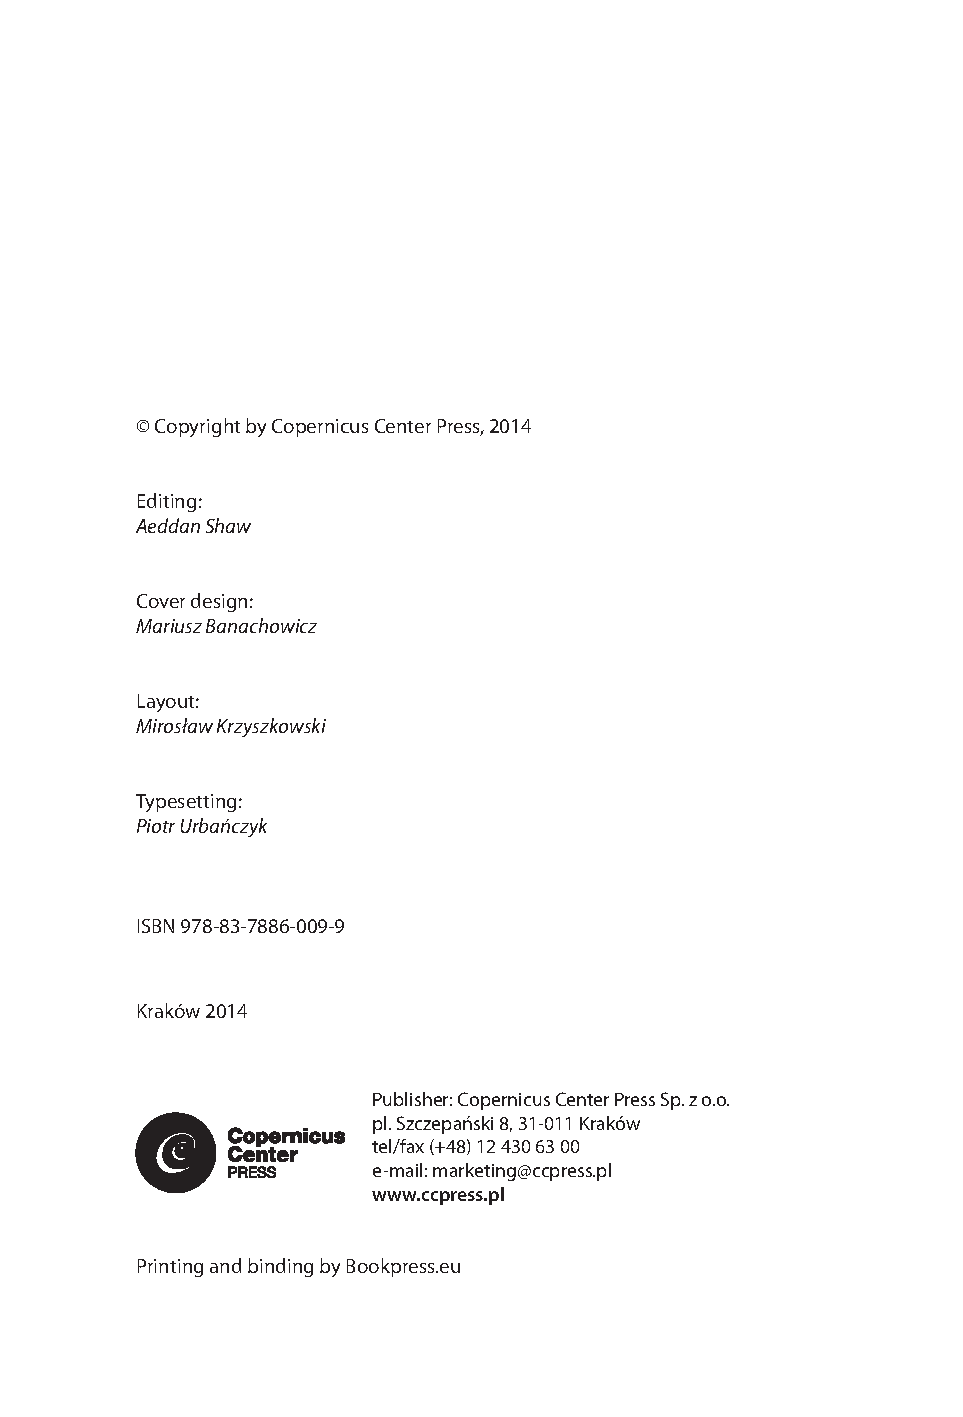
\includepdf[pages=1]{images/CT4.pdf}


\thispagestyle{empty}
\vspace*{1.2in}%
\begin{flushright}
\rectitle{Zagadnienia Filozoficzne\\w Nauce}\par
\vspace*{.5in}%
\chaptitleeng{Philosophical Problems\\in Science}\par
\end{flushright}
\vfill
\clearpage

\thispagestyle{empty}

\vfill

\noindent\begin{czw}© Copernicus Center Press, \rok\end{czw}

\vfill

\begin{adres}
	\begin{pagname}\noindent\begin{czwad}Editorial Board\end{czwad}\\
		Editor-in-Chief: dr hab. Paweł Jan Polak\\
		Deputy Editor-in-Chief: dr hab. Janusz Mączka\\
		Honorary Editor: prof. dr hab. Michał Heller\\
%		Guest Editor: dr Tomasz Kwarciński\\
		Editorial Secretary: Piotr Urbańczyk
		
	\end{pagname}
\end{adres}


\vfill

\noindent\begin{czw}Cover design: Mariusz Banachowicz\end{czw}

\vskip.5em

\noindent\begin{czw}Adjustment and correction: Artur Figarski\end{czw}

\vskip.5em

\noindent\begin{czw}Technical editor: Artur Figarski\end{czw}

\vskip.5em

\noindent\begin{czw}Typographic design: Piotr Urbańczyk\end{czw}

\vskip.5em

\noindent\begin{czw}Typeset in \end{czw}\LaTeX

%\noindent\begin{czw}Skład: Artur Figarski\end{czw}


\vfill

\begin{adres}
	\begin{pagname}\noindent ISSN 0867-8286 (print format)\\
		e-ISSN 2451-0602 (electronic format)
	\end{pagname}
\end{adres}

\vfill

\begin{adres}
		\noindent\begin{czwad}Editorial Office\end{czwad}
	
		\noindent\begin{pagname}Zagadnienia Filozoficzne w Nauce
		
		\noindent Wydział Filozoficzny UPJPII
		
		\noindent ul. Kanonicza 9, 31-002 Kraków
		
		\noindent POLAND
		
		\vskip.3em
		
		\noindent e-mail: zagadnienia@upjp2.edu.pl
		
		\noindent www.zfn.edu.pl\end{pagname}
\end{adres}

\vfill

\begin{wrapfigure}{L}{.3\textwidth}
	\noindent\includegraphics[width=.29\textwidth]{images/ccp.pdf}
%\noindent\includegraphics[width=.27\textwidth]{images/ccp.pdf}
\end{wrapfigure}
\vskip.4em
%\noindent\parbox[t]{6cm}{
\begin{adres}
	\noindent\begin{pagname}Publisher: Copernicus Center Press Sp. z o.o.
		
		\noindent pl. Szczepański 8, 31-011 Kraków POLAND
		
		\noindent tel. (+48) 12 448 14 12
		
		\noindent e-mail: marketing@ccpress.pl
		
		\noindent www.ccpress.pl\\ \end{pagname}
	
	
\end{adres}
%}




\clearpage

%	\thispagestyle{empty}
	\begin{flushright}%
	{\bigtitle{Zagadinienia\\Filozoficzne\\w Nauce\par}}%
	\vspace{0.2in}%
	{\chaptitleeng{Philosophical Problems in Science\par}}%
	\vspace{0.2in}%
	\hrule%
	{\LARGE\textbf{{\numerrzymski -- \rok}}}%
	\hrule%
	\end{flushright}%
%		\@mkboth{\czwit\contentsname}{\czwit\contentsname}%
	\vspace{0.5in}%
%
%\clearpage

%Spis tresci -------------------------------------------------

{\thispagestyle{plain} \tableofcontents \clearpage}
%--------------------------------------------------------------------------------------------
\newpage
\thispagestyle{plain}
\cleardoublepage
\thispagestyle{plain}

%--------------------------------------






%\ramkaart{Imię Nazwisko}
{Tytuł rozdziału.\\\chapsubtit{Podtytuł rozdziału}}
{Tytuł rozdziału. Podtytuł rozdziału}
{Tytuł rozdziału. Podtytuł rozdziału}

\lettrine[loversize=0.13,lines=2,lraise=0.00,nindent=0em,findent=0.2pt]%
{W}{}ielu filozofów i językoznawców twierdziło, że gdy identyfikujemy przedmioty, zarówno w języku, jak i w postrzeganiu, kierujemy się względami praktycznymi, potrzebami, wolą -- krótko mówiąc, swego rodzaju interesem, czy to gatunkowym (a więc ogólnoludzkim), czy to swoistym dla danej społeczności, cywilizacji czy jednostki. Wydaje się to kłócić z przeświadczeniem, że te przedmioty muszą istnieć, chyba że traktujemy to przeświadczenie jako jedną z wielu równouprawnionych wizji świata. Ta sama zasada wielości równosilnych perspektyw stosuje się a fortiori do języka metafizyki.

Tak więc powracamy tam, gdzie nasz horror bierze swój początek. Jakże mam trwać przy danym języku (czy jakimś szczególnym punkcie widzenia, z którego patrzę na świat, albo regule interpretacji całości doświadczenia), nie przyznając mu uprzywilejowanej poznawczej mocy? A jeśli pretenduję do dysponowania wyższym czy może nawet absolutnym językiem, to albo nadawałby się on tylko do mówienia o innych językach, nie zaś o rzeczywistości, do której się odnoszą, albo byłby standardowym językiem, a inne byłyby jego niekompletnymi dialektami. W tym drugim przypadku byłby to rzeczywiście boski język, absolutny i zawierający wszelkie wyobrażalne punkty widzenia. Lecz język taki jest niemożliwy; nawet Bóg, przemawiając ustami proroka, musiał się przełożyć na język ludzki; przekład jest niechybnie zniekształcony, a nam brak dostępu do oryginału. W przypadku pierwszym język mój (język pierwszego stopnia, język rzeczy) nie może wprawdzie rościć sobie pretensji do jakiejkolwiek pozycji uprzywilejowanej, lecz w tym języku nie sposób byłoby nieobecność owej pozycji wyrazić: by to uczynić, musiałbym swój język porzucić i przejść do super(czy meta-) języka -- ale w takim języku moje stanowisko, jako że szczególne, nie dałoby się wyrazić.

\myquote{
Gdy więc wielkodusznie powiadam: „wszystkie stanowiska metafizyczne są równie dobre”, sam żadnego stanowiska nie zajmuję, po prostu wyrażam zasadę tolerancji, która, jakkolwiek chwalebna, ma charakter formalny i nigdy nie wyda, czy choćby zainspiruje, żadnej metafizycznej idei. Lecz próbując zachować tę zasadę i obstawać zarazem przy swym szczególnym punkcie widzenia, popadam w niekonsekwencję, jako że twierdzę wtedy, iż „stanowisko moje jest tak samo dobre jak każde inne, mimo że jest nie do pogodzenia z żadnym innym”.

A jeśli tak mówię, nie mogę w zrozumiały sposób wyjaśnić, w jakim sensie to stanowisko jest moje, w przeciwieństwie do innych. Niestety, tolerancyjna wspaniałomyślność nie pozwala uciec od paradoksu samoodniesienia.
}

\noindent Leon Chwistek, logik i malarz, w wydanej w 1921 roku książce Wielość rzeczywistości sugerował istnienie czterech rodzajów wzajemnie niezależnych (a zatem przypuszczalnie nieinterferujących z sobą wzajem) rzeczywistości: rzeczy, takie jak je postrzega zdrowy rozsądek; rzeczy nauk fizycznych; wrażeń; i wyobraźni. Znajdują one swój artystyczny wyraz w malarstwie – odpowiednio: prymitywistycznym, naturalistycznym, impresjonistycznym, futurystycznym\footnote{To jest przypis dolny. Jeśli niezależne od siebie pokłady rzeczywistości wymagają dla swego opisu niezależnych języków, sugeruje to, że języki te są całkowicie nieprzekładalne; skoro tak, to w istocie można sądzić, że różne wizje świata współistnieć mogą w doskonałej wzajemnej obojętności}. Lecz wielość ta, dowodził, pozwala na dowolną liczbę równoprawnych poglądów na świat, z których żadnego nie można dowieść, lecz każdy jest do przyjęcia pod warunkiem, że nie próbuje zmonopolizować prawdy. Dopuszczalne stają się różne odpowiedzi na tradycyjne pytania, jak te o wolność woli, relację między ciałem a duchem, obiektywność wartości, jeśli zakres odniesienia ogranicza się do jednej lub niektórych spośród owych czterech rzeczywistości.

\noindent Leon Chwistek, logik i malarz, w wydanej w 1921 roku książce Wielość rzeczywistości sugerował istnienie czterech rodzajów wzajemnie niezależnych (a zatem przypuszczalnie
nieinterferujących z sobą wzajem) rzeczywistości: rzeczy, takie jak je postrzega zdrowy rozsądek

\section{Podtytuł 1 stopnia}

\noindent Teoria wielu -- jakkolwiek wyodrębnianych -- rzeczywistości, jeśli nawet w tym przypadku stworzona dla metafizycznej interpretacji malarstwa, proponuje przekonujący i kuszący obraz świata. Jednakże jako propozycja epistemologiczna nie jest w stanie -- czy to w wersji Chwistka, czy Williama Jamesa -- poradzić sobie z wciąż tą samą trudnością: jak dowieść wyższości pewnej teorii bytu w tym samym języku, w którym została wypowiedziana? Mieliżbyśmy utrzymywać, że twierdzenie „wszystko jest konieczne” jest równie prawomocne co twierdzenie „poza związkami logicznymi nic nie jest konieczne” i że doktryna, według której słowo „ja” nie ma odniesienia, jest nie mniej prawdziwa niż ta, wedle której cokolwiek ma odniesienie, jest względne w stosunku do „ja”?

\subsection{Podtytuł 2 stopnia}

\noindent Jeśli niezależne od siebie pokłady rzeczywistości wymagają dla swego opisu niezależnych języków, sugeruje to, że języki te są całkowicie nieprzekładalne; skoro tak, to w istocie można sądzić, że różne wizje świata współistnieć mogą w doskonałej wzajemnej obojętności: nie mogą być ze sobą konfrontowane ani między sobą sprzeczne. Ale twierdzenie, że nie mogą być konfrontowane, jest wyrażone w języku innym, wyższego stopnia, nie nadającym się do celów metafizycznych. I tu powraca ten sam kłopot: albo ograniczamy się do tego wyższego języka i wtedy werdykty nasze nie mają znaczenia dla rzeczywistych problemów, z których filozofia żyje, albo przyjmujemy pewną metafizyczną perspektywę i głosimy, że perspektywy tej, jako zamkniętej, nie da się zharmonizować z żadną inną ani też innej przeciwstawić -- i wtedy też, w wyniku tej samointerpretacji, perspektywa nasza jest bez znaczenia dla rzeczywistych problemów, z których filozofia żyje.

\sectionno{Podtytuł 1 stopnia}

\noindent Teoria wielu -- jakkolwiek wyodrębnianych -- rzeczywistości, jeśli nawet w tym przypadku stworzona dla metafizycznej interpretacji malarstwa, proponuje przekonujący i kuszący obraz świata. Jednakże jako propozycja epistemologiczna nie jest w stanie -- czy to w wersji Chwistka, czy Williama Jamesa -- poradzić sobie z wciąż tą samą trudnością: jak dowieść wyższości pewnej teorii bytu w tym samym języku, w którym została wypowiedziana? Mieliżbyśmy utrzymywać, że twierdzenie „wszystko jest konieczne” jest równie prawomocne co twierdzenie „poza związkami logicznymi nic nie jest konieczne” i że doktryna, według której słowo „ja” nie ma odniesienia, jest nie mniej prawdziwa niż ta, wedle której cokolwiek ma odniesienie, jest względne w stosunku do „ja”?

\subsection{Podtytuł 2 stopnia}

\noindent Jeśli niezależne od siebie pokłady rzeczywistości wymagają dla swego opisu niezależnych języków, sugeruje to, że języki te są całkowicie nieprzekładalne; skoro tak, to w istocie można sądzić, że różne wizje świata współistnieć mogą w doskonałej wzajemnej obojętności: nie mogą być ze sobą konfrontowane ani między sobą sprzeczne. Ale twierdzenie, że nie mogą być konfrontowane, jest wyrażone w języku innym, wyższego stopnia, nie nadającym się do celów metafizycznych. I tu powraca ten sam kłopot: albo ograniczamy się do tego wyższego języka i wtedy werdykty nasze nie mają znaczenia dla rzeczywistych problemów, z których filozofia żyje, albo przyjmujemy pewną metafizyczną perspektywę i głosimy, że perspektywy tej, jako zamkniętej, nie da się zharmonizować z żadną inną ani też innej przeciwstawić -- i wtedy też, w wyniku tej samointerpretacji, perspektywa nasza jest bez znaczenia dla rzeczywistych problemów, z których filozofia żyje.

\section{Podtytuł 1 stopnia}

\noindent Teoria wielu -- jakkolwiek wyodrębnianych -- rzeczywistości, jeśli nawet w tym przypadku stworzona dla metafizycznej interpretacji malarstwa, proponuje przekonujący i kuszący obraz świata. Jednakże jako propozycja epistemologiczna nie jest w stanie -- czy to w wersji Chwistka, czy Williama Jamesa -- poradzić sobie z wciąż tą samą trudnością: jak dowieść wyższości pewnej teorii bytu w tym samym języku, w którym została wypowiedziana? Mieliżbyśmy utrzymywać, że twierdzenie „wszystko jest konieczne” jest równie prawomocne co twierdzenie „poza związkami logicznymi nic nie jest konieczne” i że doktryna, według której słowo „ja” nie ma odniesienia, jest nie mniej prawdziwa niż ta, wedle której cokolwiek ma odniesienie, jest względne w stosunku do „ja”?

\subsection{Podtytuł 2 stopnia}

\noindent Jeśli niezależne od siebie pokłady rzeczywistości wymagają dla swego opisu niezależnych języków, sugeruje to, że języki te są całkowicie nieprzekładalne; skoro tak, to w istocie można sądzić, że różne wizje świata współistnieć mogą w doskonałej wzajemnej obojętności: nie mogą być ze sobą konfrontowane ani między sobą sprzeczne. Ale twierdzenie, że nie mogą być konfrontowane, jest wyrażone w języku innym, wyższego stopnia, nie nadającym się do celów metafizycznych. I tu powraca ten sam kłopot: albo ograniczamy się do tego wyższego języka i wtedy werdykty nasze nie mają znaczenia dla rzeczywistych problemów, z których filozofia żyje, albo przyjmujemy pewną metafizyczną perspektywę i głosimy, że perspektywy tej, jako zamkniętej, nie da się zharmonizować z żadną inną ani też innej przeciwstawić -- i wtedy też, w wyniku tej samointerpretacji, perspektywa nasza jest bez znaczenia dla rzeczywistych problemów, z których filozofia żyje.

\begin{thebibliography}{00}{Imię Nazwisko}
{Tytuł rozdziału. Podtytuł rozdziału}

\makeatletter
    \clubpenalty10000
    \@clubpenalty \clubpenalty
    \widowpenalty10000
\makeatother


\bibitem{Abc}
A.~Abc, \textit{Abc}...

\bibitem{Xyz}
A.~Abc, \textit{Abc}...

\end{thebibliography}





%\sekcja{Od Redakcji}{Editorial}

%\input{EDI_Kwarcinski/Kwarcinski.tex}



\sekcja{Artykuły}{Articles}

%EN

\begin{artengenv}{Jerzy Dadaczyński, Robert Piechowicz}
	{Maxime Bôcher's concept of complementary philosophy of mathematics}
	{Maxime Bôcher's concept of complementary philosophy of mathematics}
	{Maxime Bôcher's concept of complementary philosophy\\of mathematics}
	{Pontifical University of John Paul II in Krakow}
	{The main purpose of the present paper is to demonstrate that as early as 1904 pre-eminent American mathematician Maxime Bôcher was an adherent to the presently relevant argument of reasonableness, or even necessity of parallel development of two philosophical methods of reflection on mathematics, so that its essence could be more fully comprehended. The goal of the research gives rise to the question: what two types of philosophical deliberation on mathematics were proposed by Bôcher?}
	{philosophy, mathematics, Maxim Bôcher, metamathematics.}
	




\section{Introduction}
\lettrine[loversize=0.13,lines=2,lraise=-0.05,nindent=0em,findent=0.2pt]%
{T}{}he main purpose of the present paper is to demonstrate that as early as 1904 pre-eminent American mathematician Maxime Bôcher\footnote{Maxime Bôcher (1867-1918) was a son of an American scientist of French origin. In the years 1883-1888 he studied, \textit{inter alia}, mathematics at Harvard. In the years 1888-1891, in Göttingen he was a student of Klein's, under the direction of whom he wrote and defended his doctoral dissertation. After his return to the USA he was an assistant professor, and as of 1904 a professor of mathematics at Harvard. In the years 1909-1910 he served as president of the American Mathematical Society. Bôcher specialised chiefly in mathematical analysis, and his most famous paper is \textit{Introduction to Higher Algebra}
%\label{ref:RNDc7ZxUmWWTi}(Bôcher, 1907).
\parencite[][]{bocher_introduction_1907}.
To honour the memory of this mathematician, who died prematurely, Bôcher Memorial Prize was endowed; it is awarded at intervals of several years for achievements in the field of mathematical analysis in the period of the six years leading up to the prize-giving year. One of the prize-winners was von Neumann (in the 1930s).} was an adherent to the presently relevant argument of reasonableness, or even necessity of parallel development of two philosophical---complementary---methods of reflection on mathematics, so that its essence could be more fully comprehended.

Thus outlined, the main goal of the research gives rise to the question: what two---complementary---types of philosophical deliberation on mathematics were proposed by Bôcher? They were ``adumbrated'' in the text entitled \textit{The Fundamental Conceptions and Methods of Mathematics}
%\label{ref:RNDNx8Z5TUKyi}(Bôcher, 1904).
\parencite[][]{bocher_fundamental_1904}.


In the first, principal part of his text---which has already been analysed in
%\label{ref:RNDBGQjug7NKV}(Dadaczyński, 2015)
\parencite[][]{dadaczynski_tendencje_2015}---Bôcher made a direct reference to logicism, proposing its corrections, so that the reductionist programme could be appropriately realised.\footnote{Bôcher was doubtful as to the possibility of realising the programme of logicism the way it had been delineated by Frege and Russell. His objection was that logic---as viewed by the originators of logicism---was too ``weak'' to ``produce'' an infinite set of natural numbers. Bôcher's predictions proved right while work on \textit{Principia Mathematica} was underway: it was necessary to ``add'' some form of an axiom of infinity---in the ontological version providing for the existence of an infinitude of individuals---to obtain natural numbers (of any type). Such an axiom did not ``fit within'' Frege's logic or Russell's ``starting'' logic. The American mathematician formulated his objections as follows: ``Nevertheless, in view of the fact that the system of finite positive integers is necessary in almost all branches of mathematics (we cannot speak of a triangle or a hexagon without having the numbers three and six at our disposal), it seems extremely desirable that the system of logical principles which we lay at the foundation of all mathematics be assumed, if possible, broad enough so that the existence of positive integers---at least finite integers---follows from it; and there seems little doubt that this can be done in a satisfactory manner. When this has been done we shall perhaps be able to regard, with Russell, pure mathematics as consisting exclusively of deductions by ‘logical principles from logical principles'' 
%\label{ref:RNDHPWwCxIM4I}(Bôcher, 1904, p.132).
\parencite[][p.132]{bocher_fundamental_1904}.%
} He made an \textit{explicite} demand for future demonstration of non-contradiction of all mathematics liberated---and such liberation he anticipated---of known antinomies, and not just ``partial'' demands for proof of non-contradiction of the arithmetic of real numbers 
%\label{ref:RNDwQcEhP4x06}(Hilbert, 1900),
\parencite[][]{hilbert_uber_1900},
or the arithmetic of natural numbers 
%\label{ref:RNDQN0fkQatZT}(Hilbert, 1905).
\parencite[][]{hilbert_uber_1905}.
In a sense---which was demonstrated in the paper 
%\label{ref:RND8LFBlHFrCY}(Dadaczyński, 2015)
\parencite[][]{dadaczynski_tendencje_2015}---the first part of Bôcher's text contains, \textit{inter alia}, an ``outline,'' though an unordered one, of the 1904 state of philosophy of mathematics confederated with the study of its foundations.\footnote{The passage below serves to bring back the conclusions from the paper 
%\label{ref:RNDLccZyjKs8M}(Dadaczyński, 2015).
\parencite[][]{dadaczynski_tendencje_2015}.
 In 1904 logicism was already a well-developed direction in the study of the foundations of mathematics. Bôcher could see its intrinsic difficulties concerned with the establishment of antinomies, but he was sure that corrections of the logic underlying the foundations of mathematics would make it possible to remove those difficulties. Hence, in a sense, he ``announced'' the ``second'' logicism---the one of Russell's. Two points excerpted from the 1904 text foreshadowed Hilbert's formalism of the 1920s. They are, firstly, methodical nominalism, and, secondly, posing a question whether it is possible to establish---having removed known antinomies---a global non-contradiction of mathematics. The latter issue was Bôcher's clear reference to Hilbert's second problem (non-contradiction of the arithmetic of real numbers) and Hilbert's first attempts at proving the non-contradiction of the arithmetic of natural numbers. The positive solution to the problem of the global non-contradiction of mathematics---which was emphasised by, \textit{inter alia}, Bôcher---later on became the goal of the formalist research programme, the attainment of which being the rationale for the emergence of metamathematics. Methodological nominalism became Hilbert's answer to the question about semantics of the fully axiomatised and formalised classical mathematics. Bôcher's text of 1904 negatively treats Kantianism as the foundation on which to construct mathematics. Nevertheless, it is a source that confirms that Kantianism was still relevant in many mathematical milieus in the early 20\textsuperscript{th} century. That was the ground on which, several years after the publication of Bôcher's text and following the adoption of appropriate corrections and modifications, intuitionism emerged.} Noteworthily, Bôcher termed his own way of deliberating over mathematics, which he presented in the first, principal part of his work, ``discussion [...] of the so-called foundations'' 
%\label{ref:RNDTfXSIWcrjs}(Bôcher, 1904, pp.132–133),
\parencite[][pp.132–133]{bocher_fundamental_1904},
 which focuses on the deductive aspect of mathematics. His---to use his own term---``discussion [...] of the so-called foundations'' of mathematics, in which he develops some of his own threads, \textit{inter alia}, attempting to specify what mathematics is, is a kind of reflection markedly determined by the way (and ``contents'') of Frege's, Russell's and Hilbert's deliberation on mathematics.

Since the first way of deliberation on mathematics, which was proposed by Bôcher, has already been subjected to analysis and identified, demonstrating that his metaphilosophy contained a demand for inclusion of the two---complementary---types of philosophy of mathematics becomes reduced to showing that Bôcher was outlining an alternative---though naturally not in the sense of an exclusive alternative---concept of philosophical reflection on mathematics, which in his opinion was to complement philosophy confederated with the study of the foundations of mathematics.

With a view to the attainment of the above-indicated research objective, in the first place, presentation will be made of the main outlines of \textit{quasi}-empiricism---philosophy of mathematics initiated with Lakatos' publications of the first half of the 1960s. The fundamental imperatives of \textit{quasi}-empiricism shall serve here as points of reference for analysis and identification of the content of the alternative variant of philosophy of mathematics outlined by Bôcher.

This place calls for a crucial remark. Originated with Lakatos' texts, \textit{quasi}-empiricism strongly emphasised some threads of philosophy of mathematics which, although constantly present in deliberation on mathematics, for more than half a century were ``suppressed'' by study concerned with foundations (logicism, formalism and intuitionism). Mention will be made here of the prehistory of \textit{quasi}-empiricism, and one of partial propositions will be to show that Bôcher should be reckoned among its representatives. The choice of \textit{quasi}-empiricism as a point of reference for the study of an alternative thread of Bôcher's philosophy of mathematics may seem to be an ahistorical approach exactly because it does not take account of the above-mentioned chronology. However, the above measure has been chosen, because \textit{quasi}-empiricism is a popularly known version of philosophy of mathematics as an alternative to philosophy confederated with the study of foundations, and a reference to it will make it relatively easy to pinpoint the ``locus'' of the other way of deliberation on mathematics---presented by Bôcher---on the ``map'' of variants of philosophy of mathematics.

\section{An outline of \textit{quasi}-empiricism}
The beginnings of quasi-empiricism are related to a four-part paper entitled \textit{Proofs and Refutations}
%\label{ref:RNDlCDsZHJWUQ}(Lakatos, 1963),
\parencite[][]{lakatos_proofs_1963},
 which Lakatos published in ``The British Journal of the Philosophy of Science'' in 1963-1964. A coherent description of the direction originated with Lakatos' publications is not an easy task. The reason may be that it is not so much about a uniform direction in the philosophy of mathematics, as about a wave of---essentially uncoordinated---reactions to the way philosophy of mathematics had been pursued before.

It was Tymoczko who attempted a certain characterisation which consisted in enumerating some tendencies, not necessarily common to all the representatives of the ``new'' philosophy of mathematics. Amongst the manifestations of the ``new'' philosophy pointed out by Tymoczko, he mentions: focusing attention on informal proofs in mathematics and on explanation which is juxtaposed with formal proofs, the use of computers to prove mathematical theorems, the issues concerned with errors in mathematics, drawing attention to the history of mathematics, and in particular to the reconstruction of essential discoveries, addressing the issue of communication within the community of mathematicians.\footnote{,,If we look at mathematics without prejudice, many features will stand out as relevant that were ignored by the foundationalist: informal proofs, historical development, the possibility of mathematical error, mathematical explanations (in contrast to proofs), communication among mathematicians, the use of computers in modern mathematics, and many more''
%\label{ref:RNDYOKoeMEYyv}(Tymoczko, 1986, p.xvi).
\parencite[][p.xvi]{tymoczko_introduction_1986}.%
}

It appears that the manifestations of \textit{quasi}-empiricism mentioned by Tymoczko should also necessarily include two aspects of the new philosophy of mathematics which in their first presentation were strongly emphasised by I. Lakatos.

Firstly, it is about fallibility of mathematical theorems
%\label{ref:RNDEwhe4aJ9qw}(Lakatos, 1976, p.139).
\parencite[][p.139]{lakatos_proofs_1976}.%
\footnote{,,In fact Lakatos's \textit{quasi}-empiricism consists in the fallibility thesis. Although their subject matter is different, mathematical theories and empirical theories have in common the fact that they are fallible'' 
%\label{ref:RNDUrfHOQp6DB}(Koetsier, 1991, p.4).
\parencite[][p.4]{koetsier_lakatos_1991}.%
} Because since Popper attention has been paid to fallibility of statements advanced by empirical sciences, Lakatos' proposition about the fallibility of mathematical theorems is the first reason for choosing a name for the new direction in the philosophy of mathematics. Obviously, during the checking and testing stage, before they are provided with a correct ``Hilbertian'' proof, mathematical theorems are fallible.

Therefore, one can clearly see that with the scope of its investigation, the new philosophy of mathematics encompasses that which can be termed a ‘context of discovery.' And the differentiation between the context of discovery and the context of substantiation seems to provide a good tool for distinguishing a traditional philosophy of mathematics from \textit{quasi}-empiricism: while the traditional philosophy focused on the context of substantiation, the ``new'' philosophy found the context of discovery of mathematical theorems to be the fundamental object of its investigation, focusing its attention on the ``creative'' mathematician.

Secondly, Lakatos noted the reasonableness, the great relevance of the history of mathematics for studies concerned with philosophy of mathematics
%\label{ref:RNDWl4Qz050nC}(Lakatos, 1976, p.2).
\parencite[][p.2]{lakatos_proofs_1976}.
 It is not only and not so much about the reconstruction of crucial discoveries, on which Tymoczko laid so much emphasis, or about the history of the context of substantiation, which contains theorems with their correct and ready-made proofs. The emphasis was laid first and foremost on the history of the context of discovery, within which hypotheses were suggested, tested, and sometimes rejected; flawed proofs were presented for correct theorems, and if only in scientific correspondence and notes not intended for publication motives behind undertaken mathematical investigations were presented.

Understandably enough, it is interesting to ask whether the ``new'' philosophy of mathematics actually had its origins only in Lakatos' above-mentioned publications in the 1960s, or was there any pre-history to it. While asking about the pre-history of \textit{quasi}-empiricism, one should first and foremost take note of the authors who inspired Lakatos. These include Hegel, with his historism and dialectic, Popper, who emphasised the fallibility of statements made by empirical sciences, and Pólya, who specialised in heuristics of mathematics. Since the philosophy of mathematics was not among the pursuits of the former two, only the Hungarian mathematician and philosopher can be reckoned among those who originated the pre-history of \textit{quasi}-empiricism. Also, Wittgenstein, as represented by the late period of his activity, and Quine are usually mentioned. Certainly, account should also be taken of the lifework of Hadamard
%\label{ref:RNDwSdgR32pBO}(1945)
\parencite*[][]{hadamard_psychology_1945}
 and Poincaré 
%\label{ref:RNDkRcc7QWJnb}(1904),
\parencite*[][]{poincare_valeur_1904},
 who pursued, \textit{inter alia}, ``non-deductive,'' ``psychological'' aspects of mathematicians' ``output.''

Therefore, as already stated, even though the threads of the ``new'' philosophy were invariably present in the history of deliberation on mathematics, for more than half a century, until Lakatos' publications, they were ``muffled'' by philosophy confederated with the study of the foundations\footnote{It must be emphasised, once again, that the ``Creative Mathematician'' relying on intuition and imagination has never been out of interest for the philosophy of mathematics. This aspect of considering mathematics was represented by Husserl, and under his influence by the French school of philosophy of mathematics---starting from Poincaré. Husserl's phenomenology (intuition) was invoked in Gödel's attempt to explain the ``perception'' of the objective infinite hierarchy of infinite sets. However, none of them stressed as strongly the fallibility of the theorems of the mathematics as Bôcher and Lakatos did. Since the thesis of the fallibility of mathematical theorems is the essence of Lakatos' \textit{quasi}-empiricism, the roots of \textit{quasi}-empiricism are to be found in Bôcher.}.

\section{Elements characteristic of the later \textit{quasi}-empiricism in Bôcher's work}
It has already been mentioned that the first, fundamental part of the text by the American mathematician is distinctly determined by the way (and in part by the ``content'') of Frege's, Russell's and Hilbert's deliberation on mathematics. This part culminates in specifying mathematics with objects it investigates and with the method applied in it. Bôcher concludes that mathematics is a science of abstract objects, where (a method of) deductive reasoning is used.\footnote{``[…] I have insisted merely on the rigidly deductive form of reasoning used and the purely abstract character of the objects considered in mathematics''
%\label{ref:RNDyycHgIMS7K}(Bôcher, 1904, p.132).
\parencite[][p.132]{bocher_fundamental_1904}.%
}

\subsection{3.0. A metaphilosophical declaration}

Once the first, main part of his work is over, Bôcher immediately goes on to state that the approach to mathematics presented in his work is a ``discussion'' of the ``so-called foundations.''\footnote{``In fact I should like to subscribe most heartily to the view that in mathematics, as elsewhere, the discussion of such fundamental matters derives its interest mainly from the importance of the theory of which they are the so-called foundations''
%\label{ref:RNDmVdNhCmc3H}(Bôcher, 1904, pp.132–133).
\parencite[][pp.132–133]{bocher_fundamental_1904}.%
} Right there and then he adds that such a perception of mathematics is of ``an extremely one-sided character.''\footnote{``I fear that many of you will think that what I have been saying is of an extremely one-sided character'' 
%\label{ref:RNDRM5C9AWYYy}(Bôcher, 1904, p.132).
\parencite[][p.132]{bocher_fundamental_1904}.%
} That is why within the text under analysis he proposes an outline of yet another way of reflection on mathematics. He titles it: ``non-deductive elements in mathematics.''\footnote{Seventh section of Bôcher's paper was entitled ``The Non-Deductive Elements in Mathematics'' 
%\label{ref:RNDVbp83L8c52}(Bôcher, 1904, p.132).
\parencite[][p.132]{bocher_fundamental_1904}.%
}

With the benefit of the above remarks as well as the very layout of Bôcher's text one can presuppose that his metaphilosophy of mathematics ``contained'' the following propositions:

\begin{enumerate}
\item The ``discussion [...] of the so-called foundations'' is a new and essential direction of reflection on mathematics.
\item However, it is extremely one-sided and inadequate for complete philosophical deliberation on mathematics;
\item That is why it needs to be complemented by another perception of mathematics, one that takes into account---to stay in keeping with Bôcher's terminology---(only) that which is non-deductive in it.
\end{enumerate}
With the benefit of the contextual terminology, which was introduced before, and the remark whereby logicism, formalism and intuitionism were focused on the study of the context of substantiation in mathematics, as well as the results of the analyses performed in the paper
%\label{ref:RND15HRIVaRP6}(Dadaczyński, 2015),
\parencite[][]{dadaczynski_tendencje_2015},
 one can say that what Bôcher outlines in the first part of his work---as an approach to mathematics that is a ``discussion [...] of the so-called foundations''---is in fact a (one-sided) proposal to study the context of substantiation. This context can also be referred to as---to elaborate Bôcher's terminology (the term ``non-deductive'' to be specific) –a deductive aspect of mathematics.

The alternative reflection on mathematics proposed by Bôcher is supposed to take into account---according to his metaphilosophical declaration---(only) a non-deductive aspect of mathematics. Further analysis in the present paper is aimed at answering the question: does the non-deductive aspect of mathematics, singled out by Bôcher, ``coincide'' with the context of discovery in mathematics?

\subsection{3.1. A ``creative mathematician''---significance of imagination}

Bôcher begins his characterisation of the non-deductive elements of mathematics with a comparison. He writes that he likes to perceive mathematics as more of an art than science. In his opinion, a mathematician is an artist led by, though not controlled, by the external, sensual world. Creativity thus construed bears a real resemblance to the activity engaged in by an artist, e.g. a painter. Bôcher likens the mathematician's capacity to pursue deductive reasoning to the artist's skill at mastering painting techniques. When properly developed, the said capacity is a \textit{sine qua non} for being a mathematician, just like the skill at mastering suitable painting techniques is a \textit{sine qua non} for becoming a painter. However, these capabilities are not sufficient conditions for becoming either a ``full-blooded'' mathematician or a ``full-blooded'' painter; what is more---in Bôcher's opinion---they are not even the most important skills conditioning becoming either of the two. Other predispositions play a crucial role, but above all imagination---in both cases---is a more vital factor ``making'' someone a ``good mathematician'' or a ``good painter.''\footnote{``I like to look at mathematics almost more as an art than as a science; for the activity of the mathematician, constantly creating as he is, guided though not controlled by the external world of the senses, bears a resemblance, not fanciful I believe but real, to the activity of an artist, of a painter let us say. Rigorous deductive reasoning on the part of the mathematician may be likened here to technical skill in drawing on the part of the painter. Just as no one can become a good painter without a certain amount of this skill, so no one can become a mathematician without the power to reason accurately up to a certain point. Yet these qualities, fundamental though they are, do not make a painter or a mathematician worthy of the name, nor indeed are they the most important factors in the case. Other qualities of a far more subtle sort, chief among which in both cases is imagination, go to the making of the good artist or good mathematician''
%\label{ref:RNDfe2UhwlTxs}(Bôcher, 1904, p.133).
\parencite[][p.133]{bocher_fundamental_1904}.%
}

The fact that Bôcher regards a (good) mathematician primarily as an artist is of relevance to the research in hand. And here apparently lies the fundamental similarity between Bôcher's reflection on mathematics and later reflection by many representatives of \textit{quasi}-empiricism. The latter ones were primarily interested in the ``creative'' mathematician, his process of obtaining crucial results. They tried to describe the ``creative'' mathematician and to isolate---as far as possible---the procedures constituting mathematical creativity.

In his brief outline of the issue, Bôcher undertakes essentially the same task. His results could be summarised as follows: mathematics is more of an art than science; there are real similarities between the mathematician's work and the work done by an artist (e.g. a painter); in both cases it is (creative) imagination that is of crucial relevance for the value of the results.

It needs to be noted that Bôcher does not go on to belabour the comparison between a mathematician and an artist. But it appears that further conclusions with regard to the ``creative'' mathematician might be drawn from this comparison. Bôcher merely remarks that such a perception of the ``creative'' mathematician essentially allows for introduction of the notion of value among the instruments for evaluating mathematical achievements, just like it is done when evaluating a work of art.\footnote{,,Other qualities of a far more subtle sort, chief among which in both cases is imagination, go to the making of the good artist or good mathematician. I must content myself by merely recalling to you this somewhat vague and difficult though interesting field of speculation which arises when we attempt to attach \textit{value} to mathematical work, a field which is familiar enough to us all in the analogous case of artistic or literary criticism''
%\label{ref:RNDp1pZGnaAyW}(Bôcher, 1904, p.133).
\parencite[][p.133]{bocher_fundamental_1904}.%
} He himself speaks about a ``good mathematician'' in the sense in which one speaks about a ``good artist.''

In this case Bôcher does not follow up on the thread. With the expression of a ``good mathematician'' he suggests that a ``creative'' mathematician should be subjected to assessment, but obviously the assessment must be made by means of evaluating his creative output, that is by means of evaluating ``created'' mathematical objects, their entire structures and perceived properties of these objects, captured in the form of theorems, or alternatively hypotheses. One might only surmise that an evaluation of a mathematician's ``product'' could include such criteria as: boldness, conventionality/unconventionality, a (new) perspective when approaching the existing issues, a level of abstraction.

At any rate---and this should be strongly emphasised---given the present study indicating that Bôcher addressed essential threads characteristic of the much later \textit{quasi}-empiricism, it is vital to show that Bôcher stressed the question of a ``creative'' mathematician, which was of such great import for that direction. One might add that it was exactly addressing this issue that later on came to bear on the shift of emphasis in the philosophy of mathematics effected by representatives of \textit{quasi}-empiricism in relation to the earlier philosophy of mathematics pursued in ``the spirit of foundations.''

But it is exactly the latter statement that is potentially debatable. After all, it was within the framework of intuitionism---as well as other constructivist trends---that unusually dogmatic emphasis was placed on the issues concerned with creation---constructing mathematical objects. And it was the subject who was supposed to do the constructing.

However, leaving aside the fact that there was no consensus with regard to specifying the construction, it must be concluded that within the framework of intuitionism there was no answer to the question: how does the subject (mathematician) do the constructing, and to be more precise, what are the subjective determinants of being a ``creative'' (constructing) mathematician. It was exactly these questions that were posed, and attempts were made at answering them within the framework of \textit{quasi}-empiricism and in Bôcher's text. Besides, constructivism would sometimes even ``hinder'' intuitionists by generating ``proof-theory'' restrictions. It is sufficient to point to the rejection---for constructivist reasons---of indirect proofs of existential theorems. A mathematician hindered by those principles certainly did not match the vision of a ``liberated'' mathematician-artist as outlined by Bôcher.

\subsection{3.2. Intuition}

As he goes on describing an alternative way of reflection on mathematics, which is different from the perception of mathematics from the perspective of the ``so-called foundations,'' Bôcher notes the role of intuition among the instruments used by a ``creative'' mathematician. But here his remarks are only sketchy. As a matter of fact, he only singles out geometric, mechanical and physical intuition, saying that the significance of intuition among the instruments used by a creative mathematician is so popularly known that a mere mention of it is enough.\footnote{,,A discussion and analysis of the non-deductive methods which the creative mathematician really uses would be both interesting and instructive. Here I must content myself with the enumeration of a few of them. First and foremost, there is the use of intuition, whether geometric, mechanical, or physical. The great service which this method has rendered and is still rendering to mathematics both pure and applied is so well known that a mere mention is sufficient''
%\label{ref:RND4OfAwXmUjB}(Bôcher, 1904, p.134).
\parencite[][p.134]{bocher_fundamental_1904}.%
}

Bôcher wrote the text before the emergence of intuitionism, in which (pre-)intuitionism of time takes on a special significance as a reference to the Kantian \textit{a priori} forms of immediacy of time, and is supposed to be the only \textit{a priori} on which Brouwer was trying to construct his mathematics. That is why as one tries to clarify the meaning of the term \textit{intuition} in Bôcher's work, one should refer to his traditional, epistemological meanings which had accompanied the term already in Descartes' and Leibniz's works. It is about direct, non-discursive cognition, and sometimes even about something that can be termed intellectual obviousness. Leaving aside the classical terminology, one could even speak about a skill at guessing, or ``seeing'' mathematical states of affairs expressed only later on with the aid of theorems and proofs appended (discursive cognition), or about some kind of a mathematical ``nose.''

At any rate, with regard to the present discussion, it is essential to state that in reflection on mathematics, from an alternative viewpoint in relation to the perception of mathematics from the perspective of the ``so-called foundations,'' Bôcher very firmly called for inclusion of such a crucial element as intuition among the instruments used by a creative mathematician.

\subsection{3.3. Experiments in mathematics}

In his alternative perception of mathematics, Bôcher takes account of the role of experiment, which he finds to be essential, in a mathematician's working practices. It must be firmly stressed that in one sentence he writes about both physical experiments (in a laboratory) and arithmetic experiments, and in both cases he uses the same English term of \textit{experiment}
%\label{ref:RNDHHiG9oGXtb}(Bôcher, 1904, p.134).
\parencite[][p.134]{bocher_fundamental_1904}.
 Therefore, it is reasonable to conclude that he could see, just like Lakatos later on, some essential relations between the (laboratory) procedures applied in physics and some procedures adopted in arithmetic.

Bôcher stresses that he means above all experiments in number theory (as well as in analysis). He says that experiment records---which, as one might believe, corroborate some statements (hypotheses) in number theory---often used to be contained in mathematicians' publications. He goes on to add that the fact that in his times the practice of publishing the records of such activities was abandoned does not change, in his opinion, the fact that an arithmetical experiment---one might add: in the context of mathematical discovery (to be more precise: of a number-theory character), in study practice---was as common as before.\footnote{,,Then there is the method of experiment; not merely the physical experiments of the laboratory or the geometric experiments I had occasion to speak of a few minutes ago, but also arithmetical experiments, numerous examples of which are found in the theory of numbers and in analysis. The mathematicians of the past frequently used this method in their printed works. That this is now seldom done must not be taken to indicate that the method itself is not used as much as ever''
%\label{ref:RNDQdKDMpRbg8}(Bôcher, 1904, p.134).
\parencite[][p.134]{bocher_fundamental_1904}.%
}

It is worth subjecting the above statement of Bôcher's, concerned with a mathematical (number-theory) experiment, to more accurate analysis. Such an experiment often takes the following form: a number-theory statement of a form, for instance, like this:
\begin{equation}
\prod a,b,c\ (F(a,b,c) = 0),
\end{equation}
where $a$, $b$, $c$ are variables belonging to the set of natural numbers, is attributed a certain degree of probability. And then substituting concrete natural numbers for variables and performing numerical operations are used to check whether the expression contained within the universal quantifier is true.

In general, two cases are possible, and they always need to be taken into account by him who is performing the number-theory experiment: with the natural numbers substituted for the variables the expression (1) is either true, or it is not. In the first case corroboration (to use Popper's terminology) of the statement (1) takes place, while the second case is one of falsification (to use the same terminology) of the ``experimental''---and hence hypothetical---statement (1).

Falsification process for statement (1) is conducted according to the law of \textit{modus tollens}:
\begin{equation}
\begin{split}
(\prod a,b,c\ (F(a,b,c) = 0) \to F(a_{k}, b_{l}, c_{m}) = 0)\\
\land\ \neg (F(a_{k}, b_{l}, c_{m}) = 0)
\to \neg \prod a,b,c\ (F(a,b,c) = 0),
\end{split}
\end{equation}
where $a_{k}$, $b_{l}$, $c_{m}$ are fixed natural numbers.

With regard to the present study, it is essential that as Bôcher fully accepts an experiment among the mathematician's instruments, above all but not only in the field of number theory investigations, and \textit{explicite} declares its relations with a physical experiment in a laboratory, he points, \textit{implicite} – but as one might surmise consciously---to the fact that in mathematical practice some mathematical statements are accepted ``experimentally'' as hypotheses and---as one might add today: in the context of mathematical discovery---some elements of mathematical knowledge (some statements in which this knowledge is expressed) are fallible.

As demonstrated before, the statement whereby some mathematical propositions are fallible and as such may be subjected to testing was the main theorem of Lakatos' \textit{quasi}-empiricism, inspired by the thesis of fallibility of physical knowledge and the thesis of the actual application of falsification processes in the field of physics, the theses having been formulated by Popper. And therefore, by advancing---though only \textit{implicite} by addressing the relevance of an experiment in mathematics (and in particular in number theory)---the issue of fallibility of some parts of mathematical knowledge, Bôcher emphasised another crucial thesis characteristic of the later \textit{quasi}-empiricism of the 1960s.

Obviously, one should remember that experiments of this kind have featured and will always feature in some branches of mathematics. And it is no discovery by Bôcher or Lakatos. Something else is to be owed to them: pointing to the necessity to take account of mathematical experiments and hypotheses in the field of philosophical study of mathematics. Quite obviously they belong to the scope of the context of discovery, and within the study of classical directions of the philosophy of mathematics that focused on the context of substantiation they were not addressed.

\subsection{3.4. (Incomplete) induction}

Another element of Bôcher's perception of mathematics from an alternative viewpoint is about taking into account inductive reasoning that actually features among the mathematician's ``instruments.'' Bôcher writes about ``the ordinary method of induction,'' thereby distinguishing it---as one might suppose---from mathematical induction and juxtaposing it with deduction, which he used to characterise mathematics from the viewpoint of ``the so-called foundations.'' Bôcher finds that applying induction in mathematical practice is often correlated with the use of experiment, which is analysed in the present paper above.\footnote{``Closely allied to this method of experiment is the method of analogy which assumes that something true of a considerable number of cases will probably be true in analogous cases. This is, of course, nothing but the ordinary method of induction. But in mathematics induction may be employed not merely in connection with the experimental method, but also to extend results won by deductive methods to other analogous cases. This use of induction has often been unconscious and sometimes overbold, as, for instance, when the operations of ordinary algebra were extended without scruple to infinite series''
%\label{ref:RNDAcpy86tM1U}(Bôcher, 1904, p.134).
\parencite[][p.134]{bocher_fundamental_1904}.%
} Indeed, for instance in number theory---one should add: in the work done in the context of discovery---to make a certain statement probable, say one like (1), it is put to a series of tests involving concrete substitutions, which can be regarded as an application of ``ordinary'' induction.

\subsection{3.5. ``A method of optimism''}

Another element of Bôcher's alternative perception of mathematics is about taking into account that which he calls ``a method of optimism.'' It makes it possible to ``shut our eyes to the possibility of evil''---as Bôcher claims---and a rapid development of many branches of mathematics may be the benefit here. Bôcher provides the following example of the application of this method: ``I know that I have no right to divide by zero; but there are so many other values which the expression by which I am dividing might have that I will assume that the Evil One has not thrown a zero in my denominator this time.''\footnote{``Finally, there is what may perhaps be called the method of optimism which leads us either willfully or instinctively to shut our eyes to the possibility of evil. Thus the optimist who treats a problem in algebra or analytic geometry will say, if he stops to reflect on what he is doing : ‘I know that I have no right to divide by zero; but there are so many other values which the expression by which I am dividing might have that I will assume that the Evil One has not thrown a zero in my denominator this time'. This method, if a proceeding often unconscious can be called a method, has been of great service in the rapid development of many branches of mathematics, though it may well be doubted whether in a subject as highly developed as is ordinary algebra it has not now survived its usefulness''
%\label{ref:RNDP8LXuuoscK}(Bôcher, 1904, pp.134–135).
\parencite[][pp.134–135]{bocher_fundamental_1904}.%
}

In this way one can illustrate the ``method of optimism'' that Bôcher discerns in mathematical practice; in his opinion the method was instrumental in the rapid development of many branches of mathematics. Noteworthily, he notes that in many specific cases mathematicians were not aware of the application of this ``method'' as a method, as they tried to achieve projected results as quickly as possible. Bôcher goes as far as to claim that some kind of instinct might have been involved. Bearing in mind the previous remarks, one might add that the instinct might have been connected with the intuition and imagination of a mathematician who ``sees'' the goal of his actions and who believes that technical improvement of the ``road'' leading to the goal is of great but not utmost importance.

Such actions, inspired by the ``method of optimism,'' are completely different from the course of action pursued in formalism, logicism and intuitionism. The former two did not allow any ``gaps'' in proving---however, Frege lucidly defined a proof in logic, and Hilbert clearly indicated what a proof in mathematics is. Both worked with axiomatic systems, unlike Brouwer, who claimed that a subject's creative thought cannot be axiomatised. Still, the way of proving in Brouwer's intuitionism was in a sense even more restrictive and rigorous. It is sufficient to mention the rejection of indirect proofs of existential theorems on account of the fact that they did not provide the construction of the object the existence of which they were supposed to substantiate. However, it must be borne in mind that normative schools of philosophy of mathematics set themselves tasks completely different than the ``upward'' development of mathematics, or exploring its new areas. They were pursuing their own philosophical goals concerned with its foundations, and so they had to be rigorous and meticulous in their---and this needs to be strongly emphasised---reconstructions of mathematics as actually pursued.

This point calls for a recapitulation of the study conducted thus far. As early as the beginning of the 20\textsuperscript{th} century Bôcher did not hold with perceiving mathematics solely in the spirit of---to use his own expression---``the so-called foundations.''\footnote{``This explains how, again and again, it has come about, that the most important mathematical developments have taken place by methods which cannot be wholly justified by our present canons of mathematical rigor, the logical ``foundation'' having been supplied only long after the superstructure had been raised. A discussion and analysis of the non-deductive methods which the creative mathematician really uses would be both interesting and instructive''
%\label{ref:RNDBjpQdSo63Y}(Bôcher, 1904, p.134).
\parencite[][p.134]{bocher_fundamental_1904}.%
} He claimed that the analysis of the phenomenon of mathematics should also necessarily include a phenomenon of a ``creative'' mathematician. In his opinion, imagination and intuition are extremely important in the description of a ``creative'' mathematician. Owing to the former, creative pursuit of mathematics is similar to an art rather than science. He considered taking into account non-discursive cognitive methods---intuition---in the research field of philosophy of mathematics to be unquestionable. Bôcher claimed that in their quests mathematicians refer to experiments. It must be stressed that in one sentence he mentioned a physical experiment performed in a laboratory and an arithmetical experiment. His pointing to number-theory experiments makes it possible, as part of the analyses performed in the present paper, to establish that Bôcher, at least \textit{implicite}, agreed to (temporal) fallibility of some parts of (number-theory) mathematical knowledge and, in at least this scope, he accepted the application of falsification processes in mathematics. Thus, in the research field of his alternative philosophy of mathematics he included mathematical hypotheses. The American scholar pointed to the application of processes of induction---as opposed to deduction---in the practice of mathematical research. He also outlined the so-called ``method of optimism,'' which in his opinion played a really crucial role among the instruments used by mathematicians ``creating'' new mathematical disciplines.

It needs to be clearly highlighted that both emphasising the fallibility of mathematical knowledge and the ability to discern the reference in mathematics to the processes of falsification and induction, as opposed to deduction, as well as concentration on the description of the work of a ``creative'' mathematician, including his imagination and intuition, belong to the ``hard core'' of the later \textit{quasi}-empiricism.

The above statements lead to two vital---from the viewpoint of the present study---conclusions:

\begin{enumerate}
\item An alternative variant of deliberation on mathematics---outlined by Bôcher---as well as the later \textit{quasi}-empiricism, with which, as it has already been established, the variant coincides in many respects---focuses on the research into the context of discovery. By way of reference to Bôcher's terminology, one might say that the non-deductive aspect of mathematics, which he emphasised, is in essence the context of discovery.
\end{enumerate}
2. On account of the fact that Bôcher undertakes reflection on the non-deductive aspect of mathematics, he can be reckoned among the thinkers creating the pre-history of \textit{quasi}-empiricism.

\section{A ``historicised'' philosophy of mathematics}
It has been demonstrated above that Bôcher called for an alternative way of philosophical reflection on mathematics, as opposed to the ``discussion [...] of the so-called foundations,'' to use his own expression. It has been found that this way was supposed to allow for the aspects of mathematics that came to lie outside the field of research conducted in the ``spirit of foundations,'' and that the alternative philosophical proposal coincided with the trend of the philosophy of mathematics emphasised by Lakatos.

However, it is worth noting that so far in Bôcher's concept no imperative to include the history of mathematics in the alternative approach to the philosophy of mathematics has been pointed to, which was one of the component parts of \textit{quasi}-empiricism.

The explanation is as follows: As he outlined the concept of an alternative version of the philosophy of mathematics, Bôcher did not include a metaphysical demand that the results of research into the history of mathematics should be included. Nevertheless, he himself, in the text under examination, makes several references to the history of mathematics so as to consolidate the theses with regard to the proposed---alternative---philosophy of mathematics.

That is why one may claim that although Bôcher \textit{explicite} did not combine the alternative philosophy of mathematics with a metaphilosophical demand for inclusion of the history of mathematics in it, he as a matter of fact realised this demand.

An example of such realisation is a short sketch included in Bôcher's text under discussion, which shows the ways in which Cauchy's, Abel's and Weierstrass' works contributed to the consolidation of the foundations of mathematical analysis. Bôcher uses the historical reference to show how the mathematical theories which were already ``discovered,'' but were not fully ``substantiated,'' came to be consolidated. And then he ventures a more general reflection that certainly is of a philosophical character---it will be presented here with the aid of ``contextual'' terminology. Namely, Bôcher essentially concludes that the borderline between the context of discovery and the context of substantiation has not been in the history of mathematics some kind of \textit{constans}, but a changeable function of time. That is to say, in other words: the standards of that which is scientific and non-scientific, the requirements concerned with acceptance or non-acceptance of certain processes (of one proof or another) within the context of substantiation (in mathematics) are not absolute.\footnote{``We are in the habit of speaking of logical rigor and the consideration of axioms and postulates as the foundations on which the superb structure of modern mathematics rests; and it is often a matter of wonder how such a great edifice can rest securely on such a small foundation. Moreover, these foundations have not always seemed so secure as they do at present. During the first half of the nineteenth century certain mathematicians of a critical turn of mind---Cauchy, Abel, Weierstrass, to mention the greatest of them---perceived to their dismay that these foundations were not sound, and some of the best efforts of their lives were devoted to strengthening and improving them. And yet I doubt whether the great results of mathematics seemed less certain to any of them because of the weakness they perceived in the foundations on which these results are built up. The fact is that what we call mathematical rigor is merely one of the foundation stones of the science; an important and essential one surely, yet not the only thing upon which we can rely. A science which has developed along such broad lines as mathematics, with such numerous relations of its parts both to one another and to other sciences, could not long contain serious error without detection. This explains how, again and again, it has come about, that the most important mathematical developments have taken place by methods which cannot be wholly justified by our present canons of mathematical rigor, the logical ‘foundation' having been supplied only long after the superstructure had been raised''
%\label{ref:RNDucNQpwEv1l}(Bôcher, 1904, pp.133–134).
\parencite[][pp.133–134]{bocher_fundamental_1904}.%
}

At any rate, with regard to the present study, it is significant that even though Bôcher did not formulate a metaphilosophical imperative to make use of the findings of the history of mathematics in the philosophy of mathematics, in his deliberation on mathematics he made references to those findings. This serves to reinforce the thesis that Bôcher's alternative variant of the philosophy of mathematics is in essential respects coincident with the later \textit{quasi}-empiricism.

\section{Conclusion}
Taking into account the findings of the paper
%\label{ref:RNDJzGF41Hy7P}(Dadaczyński, 2015)
\parencite[][]{dadaczynski_tendencje_2015}
 and the results of the above-performed analyses, one can draw the following conclusions concerned with the ``content'' of Bôcher's metaphilosophy of mathematics:

\begin{enumerate}
\item Two aspects of mathematics ought to be distinguished: a deductive and a non-deductive one;
\item The deductive aspect of mathematics essentially coincides with the object of the normative studies concerned with the philosophy of mathematics, which emerged as late as the turn of the 19\textsuperscript{th} and 20\textsuperscript{th} centuries---by referring to the contextual terminology, it was pointed out that it was the context of substantiation;
\item The non-deductive aspect of mathematics essentially coincides with the object of study of the philosophy of mathematics determined by the later \textit{quasi}-empiricism---by referring to appropriate terminology, it was pointed out that it was the context of discovery;
\item The study of the deductive aspect is an inalienable element of deliberation on mathematics;\footnote{``I fear that many of you will think that what I have been saying is of an extremely one-sided character, for I have insisted merely on the rigidly deductive form of reasoning used and the purely abstract character of the objects considered in mathematics. These, to the great majority of mathematicians, are only the dry bones of the science. Or, to change the simile, it may perhaps be said that instead of inviting you to a feast I have merely shown you the empty dishes and explained how the feast would be served if only the dishes were filled. I fully agree with this opinion, and can only plead in excuse that my subject was the \textit{fundamental} conceptions and methods of mathematics, not the infinite variety of detail and application which give our science its real vitality''
%\label{ref:RNDiVKCDnjedh}(Bôcher, 1904, p.132).
\parencite[][p.132]{bocher_fundamental_1904}.%
}
\item Taking into account the deductive aspect (the context of substantiation) only is one-sided and inadequate for the philosophical description of the phenomenon of mathematics;
\item The philosophical deliberation on the phenomenon of mathematics should necessarily allow for the non-deductive aspect (the context of discovery);\footnote{``This explains how, again and again, it has come about, that the most important mathematical developments have taken place by methods which cannot be wholly justified by our present canons of mathematical rigor, the logical ``foundation'' having been supplied only long after the superstructure had been raised. A discussion and analysis of the non-deductive methods which the creative mathematician really uses would be both interesting and instructive''
%\label{ref:RND9yNU8hpl5N}(Bôcher, 1904, p.134).
\parencite[][p.134]{bocher_fundamental_1904}.%
}
\item Both the aspects are complementary to each other---an analysis of them provides a fuller picture of mathematics from the philosophical perspective.\footnote{``While no one of these methods can in any way compare with that of rigorous deductive reasoning as a method upon which to base mathematical results, it would be merely shutting one's eyes to the facts to deny them their place in the life of the mathematical world, not merely of the past but of today. There is now, and there always will be room in the world for good mathematicians of every grade of logical precision. It is almost equally important that the small band whose chief interest lies in accuracy and rigor should not make the mistake of despising the broader though less accurate work of the great mass of their colleagues; as that the latter should not attempt to shake themselves wholly free from the restraint the former would put upon them. The union of these two tendencies in the same individuals, as it was found, for instance, in Gauss and Cauchy, seems the only sure way of avoiding complete estrangement between mathematicians of these two types''
%\label{ref:RNDfxZs3AsNsD}(Bôcher, 1904, p.135).
\parencite[][p.135]{bocher_fundamental_1904}.%
}
\end{enumerate}
The above conclusions concerned with the ``content'' of Bôcher's metaphilosophy of mathematics lead to the conclusion that at the beginning of the 20\textsuperscript{th} century he outlined a concept of a complementary, two-aspect philosophy of mathematics.

Significantly, the study of the appropriate aspects (the deductive and the non-deductive one) suggested by Bôcher essentially coincides with those ways of deliberation on mathematics which---while keeping a suitable temporal distance from Lakatos' ``revolutionary'' publications, which not infrequently drew harsh criticism, or even negation of the normative value of non-descriptive approaches to mathematics---began to be treated (one should add: again) as complementary types of reflection, and even combined into one, complementary philosophy of mathematics.

The import of Bôcher's concept, which also results from its relevance, is by no means belittled by the fact that in the very same year when Bôcher's work was published, that is 1904, Poincaré's book
%\label{ref:RNDapLZGtW5ba}(Poincaré, 1904)
\parencite[][]{poincare_valeur_1904}
 was released in Paris; its first part contains a description of two aspects of mathematics (logic and intuition) characterised in a very similar manner, and to be more precise: aspects of mathematicians' working practices, with an addition of an emphatic, metaphilosophical imperative to include both in the deliberation on mathematics, so that its fuller image could be obtained.

It can be surmised that both the ``parallel'' concepts---of Poincaré's and Bôcher's---were a reaction to the one-sided accentuation of the ``modern'' way of pursuing the philosophy of mathematics as a ``discussion of the so-called foundations,'' which emerged at the turn of the 19\textsuperscript{th} and 20\textsuperscript{th} centuries in some leading milieus of mathematicians and philosopher-mathematicians---gathered primarily around Frege, Russell, Hilbert, as well as Italian geometricians along with Peano, and pre-intuitionists---while at the same time the milieus were exposed (at least methodologically) to indispensable aspects of mathematics as actually pursued.

\end{artengenv}



\begin{artengenv}{Roman Krzanowski}
	{Why can information not be defined as being purely epistemic?}
	{Why can information not be defined as being purely epistemic?}
	{Why can information not be defined as being purely epistemic?}
	{Pontifical University of John Paul II in Krakow, Poland}
	{The concept of information can be viewed from two perspectives, namely epistemic and ontological. In the epistemic view, information is associated with meaning, semantics, and knowledge, while in the ontological view, it is understood as structures and forms of objects. Information is most often perceived as epistemic information, yet a closer look at epistemic information reveals that this concept does not account for ontological information. This paper poses the following question: Should we select epistemic or ontological information as our primary concept of information, or should we acknowledge that both kinds of information are required for a full comprehension? The discussion here is supported by references to modern research in physics, computing, cosmology, and information sciences.}
	{information, epistemic information, ontological information, quantified models of information.}




\section{The problem of information}
\enlargethispage{\baselineskip}
This paper considers whether information should be understood as epistemic or ontological content or whether we need both concepts to fully account for the nature of information. While this paper suggests possible answers to the question and indicates some of the consequences for a particular choice, its objective is to demonstrate that both views can be argued for and that both perspectives have found recognition in scientific literature.

This discussion about the nature of information touches on many core issues of philosophy of the mind, ontology, and epistemology, and it draws in several domain-specific concepts from physics, mathematics, thermodynamics, computer science, and biology. With limited space, this paper merely outlines the issues involved, because an in-depth analysis would require an extensive dedicated study. The terms used in this paper, such as the mind, a conscious agent, meaning, and knowledge are used with very precise meanings because they can be easily misinterpreted.

\enlargethispage{\baselineskip}
We begin with a trivial observation, one that is likely the only claim about information that almost everyone agrees with: We lack a universal concept of information that satisfies everyone. We have had some very good proposals, such as Shannon's Theory of Communication (TOC) and Floridi's
%\label{ref:RNDtEsSyqPLMk}(2010b)
\parencite*[][]{floridi_philosophy_2010} %
 General Definition of Information (GDI). They all have certain flaws, however. Quantifications such as those of Shannon-Weaver-Hartley 
%\label{ref:RNDXyKjNBN8Tr}(Shannon, 1948; Shannon and Weaver, 1964; Hartley, 1928),
\parencites[][]{shannon_mathematical_1948}[][]{shannon_mathematical_1964}[][]{hartley_transmission_1928}, %
 Fisher 
%\label{ref:RND6AWtJPyT5I}(Frieden, 1998),
\parencite[][]{frieden_physics_1998}, %
Kolmogorov
%\label{ref:RNDHbUx86Yr2x}(Kolmogorov, 1965; Engl. tranls. Kolmogorov, 1968)
\parencites*[][]{kolmogorov_1965}[Engl. tranls.][]{kolmogorov_three_1968} %
and Chaitin
%\label{ref:RNDQtUjiv1ktr}(2004),
\parencite*[][]{chaitin_meta_2004}, %
 among others, are mathematical formulas denoted as information measures, but they are designed for specific purposes under specific assumptions These metrics fulfill their specific purposes exceedingly well, so they are very useful. Nevertheless, the pragmatic (and domain-specific) or operational (technical) successes of an idea does not elevate its metaphysical status. Indeed, we may say that pragmatically efficient concepts are often metaphysically neutral.\footnote{We may even say that Shannon's work on the theory of communication (TOC) has led to certain distortions regarding the concept of information, and we are still mostly living in his shadow. To be fair, the subsequent misinterpretations and distortions of the TOC were committed by his followers (against Shannon's better advice), so they were out of Shannon's hands. See Shannon's warning 
%\label{ref:RNDHqdaEtB7uS}(Shannon, 1956)
\parencite[][]{shannon_bandwagon_1956} %
 or Pierce 
%\label{ref:RNDuWQz1fBAm8}(1961).
\parencite*[][]{pierce_symbols_1961}.%
} Thus, these concepts of information are not of general import, even if they are ``interpreted'' as such. So, what about the other plentiful conceptualizations of information? Floridi's GDI is by definition a concept of semantic information. However, on looking closely at the definition, the GDI assumes the existence of a quasi-physical foundation of information, which is denoted as the \textit{infon}. The rather ambiguous explanation of this foundational \textit{infon} leaves the whole concept of the GDI rather baseless. Other less comprehensive classifications and definitions of information have not produced common classification criteria or common differentiating/classification factors, nor have they proposed generally accepted conceptualizations. They are either too divergent or too narrow, and they are often contradictory. On looking at these classifications and definitions, one may realize that the scope of the concepts associated with ``information'' is so wide that it makes this idea almost meaningless and empty. Somes elected classifications of information are summarized in Table \ref{tab1-krza}.

\begin{small}
\begin{longtable}{p{.2\textwidth}p{.7\textwidth}}
{\bfseries Study} &
{\bfseries Classes, groupings, or differentiating features}\\
Wersig and Neveling
%\label{ref:RND9rAzdzJUBh}(1975)
\parencite*[][]{wersig_phenomena_1975}%
 &
Information as:

\begin{itemize}
\item structure, independent of any human perceiving it;
\item knowledge built on the basis of perception of the structure of the world;
\item a ``message'' or the meaning of the message;
\item the effect of communication; and
\end{itemize}
\begin{itemize}
\item the process of communication.
\end{itemize}
\\
Buckland
%\label{ref:RNDayOCwph7KT}(1991)
\parencite*[][]{buckland_information_1991}%
 &
Information as:

\begin{itemize}
\item information-as-process;
\item information-as-knowledge; and
\item information-as-thing.
\end{itemize}
\\
Losee
%\label{ref:RNDYtMTYioTrX}(1997)
\parencite*[][]{losee_discipline_1997}%
 &
Information as:

\begin{itemize}
\item the meaning and use of a message, as well as knowledge;
\item a fundamental characteristic of physical systems and structures (or it is a structure);
\item related to data transmission in communication systems; and
\item an output of the process.
\end{itemize}
\\
Floridi
%\label{ref:RNDCW3YHfRBbC}(2010b)
\parencite*[][]{floridi_philosophy_2010}%
 &
Information as a multi-dimensional concept:

\begin{itemize}
\item analogue, digital or binary;
\item primary, secondary, meta-, operational, and derivative;
\end{itemize}
\\
Lenski
%\label{ref:RNDq9puCVOOqG}(2010)
\parencite*[][]{lenski_information_2010}%
 &
Information as:

\begin{itemize}
\item a difference that makes the difference;
\item the values of characteristics in the processes' output, capable of transforming structure; or
\item that which modifies a knowledge structure.
\end{itemize}
\\
Nafria
%\label{ref:RNDQ9vCxVNL0Y}(2010)
\parencite*[][]{nafria_what_2010}%
 &
Information can be described as:

\begin{itemize}
\item ontological -- epistemic;
\item semiotic (syntactic, semantic, and pragmatic); and
\item discipline-based.
\end{itemize}
\\
Adriaans
%\label{ref:RNDo3t2ph4Dmm}(2019)
\parencite*[][]{adriaans_information_2019}%
 &
Information as:

\begin{itemize}
\item quantitative (using mathematical formalism, such as Shannon's entropy, Kolmogorov, Fisher, Klir); and
\item qualitative (state of an agent).
\end{itemize}
\\
\caption{Selected classifications of information.\protect\footnotemark}\label{tab1-krza}
\footnotetext{\ This is of course not an exhaustive list of classifications, because that would be a very long list indeed. For example, John Collier
%\label{ref:RNDFiG97Feoba}(1990)
\parencite*[][]{hanson_intrinsic_1990} %
 classified theories of information into mathematical theories of information, communication theories, algorithmic or computational theories, physical information theories, and measurement theories. Giovanni Sommaruga 
%\label{ref:RNDm04ahtj4Rw}(2009),
\parencite*[][]{sommaruga_one_2009}, %
 meanwhile, proposed three classes of concepts of information: ordinary language concepts, information theoretical concepts, and formal theoretical concepts. Peter Adriaas and Johan van Benthem 
%\label{ref:RNDf3hxsWkZFe}(2008)
\parencite*[][]{adriaans_introduction_2008} %
 proposed three major concepts of information: Information-A for knowledge and logic; information-B for probabilistic and information-theoretical formulations; and Information-C for algorithmic and code-compression conceptualizations. Information-B and -C are quantified. More classifications of information can be found, but listing them all would be nonsensical, because what matters is their shared weakness.}
\end{longtable}
\end{small}



%Table 1. Selected classifications of information.\footnote{This is of course not an exhaustive list of classifications, because that would be a very long list indeed. For example, John Collier
%%\label{ref:RNDFiG97Feoba}(1990)
%\parencite*[][]{hanson_intrinsic_1990} %
% classified theories of information into mathematical theories of information, communication theories, algorithmic or computational theories, physical information theories, and measurement theories. Giovanni Sommaruga 
%%\label{ref:RNDm04ahtj4Rw}(2009),
%\parencite*[][]{sommaruga_one_2009}, %
% meanwhile, proposed three classes of concepts of information: ordinary language concepts, information theoretical concepts, and formal theoretical concepts. Peter Adriaas and Johan van Benthem 
%%\label{ref:RNDf3hxsWkZFe}(2008)
%\parencite*[][]{adriaans_introduction_2008} %
% proposed three major concepts of information: Information-A for knowledge and logic; information-B for probabilistic and information-theoretical formulations; and Information-C for algorithmic and code-compression conceptualizations. Information-B and -C are quantified. More classifications of information can be found, but listing them all would be nonsensical, because what matters is their shared weakness.}

The conclusion is rather self-evident and unilluminating (as it is rather obvious): Information is a polysemantic concept with many, often contradictory, definitions (most people writing about information report the same impression).

We claim that information can be fundamentally conceptualized as being either epistemic or ontological. This proposed ``bifocal'' view is imperfect, however. There are likely cases where it is difficult to cleanly allocate information into one of these two categories. Nevertheless, with this proposed perspective, we can generally classify most concepts of information into one of these two classes and gain a revealing perspective on the concept of information.

\section{Information: the epistemic view}
In this view point, information as a concept is centered on a human or other conscious agent.\footnote{The term ``a conscious agent'' may, in addition to human agents, include animals or artificial systems.} We call this epistemic information, emphasizing its relation to knowledge and meaning, and denote it as information\textsubscript{E} or I\textsubscript{E}. Having this kind of information in mind, Norbert Weiner states, ``Information is a name for the content of what is exchanged with the outer world as we adjust to it, and make our adjustment felt upon it''
%\label{ref:RNDHpEsscgR1G}(Wiener, 1989, p.17).
\parencite[][p.17]{wiener_human_1989}. %
 Mean while, Heinz von Foerster claims, ``Informationis a relational concept that assumes meaning only when related to the cognitive structure of the observer'' 
%\label{ref:RNDoFX1tImBWn}(Foerster, 1980, p.3).
\parencite[][p.3]{foerster_epistemology_1980}. %
 Similar opinions by scientists, philosophers, and engineers have been voiced in most of the current discussions about information. Indeed, the concept of epistemic information has seen many incarnations, so there is no single definition that is acceptable to everyone or even to some nebulous majority.\footnote{The number of supporters actually does not matter, because in philosophy, ideas are not selected through democratic voting. Quite often, the ideas rejected by the majority actually contain the truth.} Take for example, Bar-Hiller and Carnap 
%\label{ref:RNDJdZYYoz3Xq}(1953),
\parencite*[][]{bar-hillel_semantic_1953}, %
 Brookes 
%\label{ref:RNDv8u1209gNK}(1980),
\parencite*[][]{brookes_foundations_1980}, %
 Rucker 
%\label{ref:RNDUwnpSiGZYX}(2013 [first published 1987]),
\parencite*[][]{rucker_mind_2013}, %
Buckland
%\label{ref:RNDFBbCRxYBxf}(1991),
\parencite*[][]{buckland_information_1991}, %
 Devlin 
%\label{ref:RNDC7Ppqiativ}(1991),
\parencite*[][]{devlin_logic_1991}, %
 Loose 
%\label{ref:RNDIy5YdaktYf}(1997),
\parencite*[][]{losee_discipline_1997}, %
 Sveiby 
%\label{ref:RNDlmiBaGsP7W}(1998),
\parencite*[][]{sveiby_what_1998}, %
 Dretske 
%\label{ref:RNDXrcd88nVXZ}(1999),
\parencite*[][]{dretske_knowledge_1999}, %
 Casagrande 
%\label{ref:RNDbHsW02yCDd}(1999),
\parencite*[][]{casagrande_information_1999}, %
 Floridi 
%\label{ref:RNDY3y5fQOZkz}(2010a; 2010b),
\parencites*[][]{floridi_information_2010}[][]{floridi_philosophy_2010}, %
Burgin
%\label{ref:RND3PKOIxU5z8}(2003),
\parencite*[][]{burgin_information_2003}, %
 Lenski 
%\label{ref:RNDQe9M9zIHdU}(2010),
\parencite*[][]{lenski_information_2010}, %
 Vernon 
%\label{ref:RNDKFNjq4quHx}(2014),
\parencite*[][]{vernon_artificial_2014}, %
 Dasgupta 
%\label{ref:RNDeLm65IUn5D}(2016),
\parencite*[][]{dasgupta_computer_2016}, %
 or Carrol 
%\label{ref:RNDoDR06MCxpI}(2017),
\parencite*[][]{carroll_big_2017}, %
 among others. Each of these authors created a somewhat different version of epistemic information, but these different versions have several similarities. They all associate information with meaning, knowledge, or semantics,\footnote{Meaning, knowledge, and semantics are some of the terms used by different researchers in defining epistemic information.} with a common thread that allows them to be collected under one heading.\footnote{As we will see, very similar concepts to epistemic information, just more restricted in scope, have been introduced by different authors as semantic information 
%\label{ref:RNDo5bxzL9CVp}(e.g. Bar-Hillel and Carnap, 1953; Dretske, 1999),
\parencites[e.g.][]{bar-hillel_semantic_1953}[][]{dretske_knowledge_1999}, %
 control information, cognitive information 
%\label{ref:RNDCcU7wMOMj4}(Collier, 1990),
\parencite[][]{hanson_intrinsic_1990}, %
 or anthropomorphic information 
%\label{ref:RNDr3o2hny0dN}(Jadacki and Brożek, 2005).
\parencite[][]{heller_na_2005}. %
 Of course, as we have indicated, most definitions of information in the current dictionaries define information with this understanding.} Epistemic\footnote{``Epistemic […] describes anything that has some relation to knowledge'' and ``Epistemology, or the theory of knowledge, is that branch of philosophy concerned with the nature of knowledge, its possibility, scope and general basis'' 
%\label{ref:RNDnpurPUIO14}(Honderich, 1995).
\parencite[][]{honderich_oxford_1995}. %
 For a specific domain of discourse (e.g., computer systems, artificial cognitive agents), the concept of knowledge may be defined in domain-specific terms while retaining the generic meaning.} information is associated with knowledge, belief, or a communication process in its more generally and broadly understood meaning.\footnote{Meaning has many interpretations. For this study, if not otherwise stated, we follow the definition from the philosophy of language, where the term ``meaning'' denotes how language relates to the world. A review of theories of meaning is beyond the scope and purpose of this work, but an extensive list of references can be found in the work of Speaks 
%\label{ref:RNDeLKijIcAOr}(2018)
\parencite*[][]{speaks_theories_2018} %
 and other sources. } Epistemic information exists only if someone or something recognizes something as information. (Some may suggest including artificial or other biological systems, but we need to be careful what we assign epistemic processing capacities to).

Epistemic information is defined in the context of a communication system, with a sender, a receiver, and a communication process. This communication system may have many realizations
%\label{ref:RNDnVcxNYkp0z}(e.g. Cherry, 1978; Shannon, 1948; Maynard Smith, 2000; Vernon, 2014),
\parencites[e.g.][]{cherry_human_1978}[][]{shannon_mathematical_1948}[][]{maynard_smith_concept_2000}[][]{vernon_artificial_2014}, %
 but it is of the general format as described by Casti 
%\label{ref:RNDNDGGBM1oRU}(1990).
\parencite*[][]{casti_paradigms_1990}. %
 Epistemic information exists specifically in, and for, the mind, which is broadly understood as a complex of cognitive faculties, of the receiver or/and the originator.\footnote{The originator or receiver may have an extended meaning, indicating a natural (i.e., not human–made) or artificial system. We may also use the term ``cognitive system'' as a more general alternative to ``the mind.''} It exists when communicated (such as being created, sent, and received) as a message. This dependency on the sender, receiver, and their cognitive functions makes information epistemically and ontologically subjective (i.e., it makes this information dependent on something else to exist.) Thus, epistemic information is relative to the cognitive faculties of a receiver or sender. (Cognitive faculties are understood very broadly here, with the human mind at one end of the spectrum and artificial systems with sensory functions at the other end.) Epistemic information is relative to the cognitive system, so a specific interpretation of the message, meaning, and knowledge depends on the specific system. This cognitive system may be a person, an organism, or a mechanical or electronic device, depending on how broadly we want to understand cognitive functions. In most cases, a cognitive system is a receiver of information, but it may also be a sender. Received or sent information is different for a human agent, a non-human biological system (e.g., a cell, a plant, a virus, a fragment of a DNA strand), or an artificial cognitive system. Yet within a specific system, the message, meaning, and knowledge fulfill the same role or function. What this means is that definitions of what a message is, what its meaning is, and what constitutes an agent is context-dependent.

In Table \ref{tab2-krza} below, we group conceptualizations of epistemic information into those related to human cognitive agents, biological agents, artificial cognitive agents, and formal models such as logic models and quantitative models. In this classification, we assume an extended view of cognitive faculties beyond that of human agents. The classification includes the formal models of Shannon-Weaver-Hartley and related proposals, Chaitin's metric, statistical models, and Devlin's information logic (closely tied with a function of an agency).The common element in all these conceptualizations is how information is conceived as having some meaning to a receiver or sender and how information comes in a message or is communicated through a system. Note that this list is by no means exhaustive.

\begin{small}
%\renewcommand*{\arraystretch}{1.4}
\begin{longtable}{p{.2\textwidth}p{.2\textwidth}p{.5\textwidth}}
{\bfseries Category of a model} &
{\bfseries Author} &
{\bfseries Main claim}\\
Human Cognitive agent &
Paul Beyond-Davis
%\label{ref:RNDGlvlgOHxMh}(2009)
\parencite*[][]{beynon-davies_business_2009}%


Luciano Floridi
%\label{ref:RNDVODwhFTa6P}(2010b)
\parencite*[][]{floridi_philosophy_2010}%
 &
Information is data + meaning.\\
&
Gregory Bateson
%\label{ref:RNDk3Ij9qZiMx}(1979)
\parencite*[][]{bateson_mind_1979}%
 &
Information consists of differences that make a difference.\\
&
Fred Dretske
%\label{ref:RNDBbigyfPfxw}(1999)
\parencite*[][]{dretske_knowledge_1999}%
 &
Information is sharply distinguished from meaning, at least for the concept of meaning relevant to semantic studies.\\
&
Buckland
%\label{ref:RNDveMzPg3oVF}(1991)
\parencite*[][]{buckland_information_1991}%
 &
Information-as-thing, information-as-knowledge, information-as-process\\
&
Ratzan
%\label{ref:RNDIw8xPlCabx}(2004)
\parencite*[][]{ratzan_understanding_2004}%
 &
Information is meaning\\
&
Davenport
%\label{ref:RND1P7GuBJBc6}(1997)
\parencite*[][]{davenport_information_1997}%
 &
Information is ``data endowed with relevance and purpose.''\\
Biological Agent &
John Maynard Smith
%\label{ref:RNDfoMBqK8sBS}(2000)
\parencite*[][]{maynard_smith_concept_2000}%
 &
DNA transmission is equivalent to a human communication channel.\\
Artificial cognitive agent &
David Vernon
%\label{ref:RND35RDE48snR}(2014)
\parencite*[][]{vernon_artificial_2014}%
 &
Information is what an artificial cognitive system extracts from its environment.\\
Formal models

including logical and quantified models

&
Keith Devlin
%\label{ref:RNDmZpBnyGuy5}(1991)
\parencite*[][]{devlin_logic_1991}%
 &
``a fundamental form of information of relevance to that agent (a cognitive agent) is information of the form: Objects a1,…,an, have/have not property P.''\\
&
Claude Shannon
%\label{ref:RNDq5JwpFhRZV}(1948)
\parencite*[][]{shannon_mathematical_1948} %
 and other models related to Hartley-Shannon-Weaver's entropy of information &
H(X) (entropy of information in the TOC)\\
&
Solomonov \parencite*[][]{solomonoff_algorithmic_2010},
Kolmogorov \parencite*[][]{kolmogorov_1965}, %
%\label{ref:RND61d5QwkFKo}(1965; 1968),
 Chaitin \parencite*{chaitin_algorithmic_1987} &
String-complexity measures based on the UTM model\\
&
Fisher and Klir
%\label{ref:RND0hntx8ruul}(1988)
\parencite*[][]{klir_fuzzy_1988} %
 Models &
Statistical measures\\
\caption{comparison of selected epistemic concepts for information.}\label{tab2-krza}
\end{longtable}
\end{small}
%Table 2. A comparison of selected epistemic concepts for information.

In summing up we may say that epistemic information is conceptualized in a range of domains and applications. These applications include human cognitive agents, biological systems, artificial cognitive systems, and logical and formal systems. The common element in all these concepts is how information is conceived as being relative to the knowledge of the agent or cognitive system in some way. Of course, what an agent, cognition, and knowledge is also needs to be understood relative to the context. Epistemic information in any of these definitions does not exist on its own. Its presence must be recognized by a reference system (i.e., an agent or an agency with some sort of cognitive capacity).

Epistemic information is how information has been most frequently understood throughout the 20\textsuperscript{th} century, which is listed in the history books as the age of information. A reader can find others referring to this type of information as cognitive information (stressing information's dependency on cognitive systems), semantic information (stressing meaning as a defining feature of information), or more frequently just as information, adding further confusion to an already muddled concept.

\section{Information: The ontological view}
From an alternative viewpoint for information, we see information as a form or organization of nature. We do not ask, ``What is information?'' in the context of a specific domain, cognitive agent, or communication process. Instead, we conceive information as an objective, mind-independent phenomenon. We see it as something that is a part of the natural world, and people are not reference points for it. We call such a thing ontological information and denote it by information\textsubscript{O} or I\textsubscript{O}. Conceptualizing information as an ontological phenomenon is less understood and researched, yet as we will see, it is well justified.

The list of researchers conceptualizing information as something ontological includes von Weizsäcker
%\label{ref:RND3yNpLmOIrc}(1971),
\parencite*[][]{weizsacker_einheit_1971}, %
 Turek 
%\label{ref:RNDHLGEKP4yWo}(1978),
\parencite*[][]{turek_filozoficzne_1978}, %
 Mynarski 
%\label{ref:RNDK3uT51fVFS}(1981),
\parencite*[][]{mynarski_elementy_1981}, %
 Heller 
%\label{ref:RNDEiGnRM5Dqa}(1987, 2014),
\parencites*[][]{heller_ewolucja_1987}[][]{heller_elementy_2014}, %
 Collier 
%\label{ref:RNDhNirmNZN90}(1990),
\parencite*[][]{hanson_intrinsic_1990}, %
 Stonier 
%\label{ref:RNDAbdJJDpMs3}(1990),
\parencite*[][]{stonier_information_1990}, %
 Devlin 
%\label{ref:RNDu19lNSZ1MV}(1991),
\parencite*[][]{devlin_logic_1991}, %
 de Mul 
%\label{ref:RND1x6iRO1eGZ}(1999),
\parencite*[][]{mul_informatization_1999}, %
 Polkinghorne 
%\label{ref:RNDP9eSMgIlFj}(2000),
\parencite*[][]{polkinghorne_faith_2000}, %
 Jadacki and Brożek 
%\label{ref:RNDx0ZXJyw7x7}(2005),
\parencite*[][]{heller_na_2005}, %
 von Baeyer 
%\label{ref:RNDRbIAVJO6PP}(2005),
\parencite*[][]{baeyer_information_2005}, %
 Seife 
%\label{ref:RNDqlXKnOK6lZ}(2006),
\parencite*[][]{seife_decoding_2006}, %
 Dodig-Crnkovic 
%\label{ref:RNDO0pNiz5UW1}(2012),
\parencite*[][]{dodig-crnkovic_alan_2012}, %
 Hidalgo 
%\label{ref:RNDIAxCPCzKat}(2015),
\parencite*[][]{hidalgo_why_2015}, %
 Wilczek 
%\label{ref:RNDrWE8RTy2FQ}(2015),
\parencite*[][]{wilczek_beautiful_2015}, %
 Rovelli 
%\label{ref:RNDqekLNMIb1Q}(2016),
\parencite*[][]{rovelli_meaning_2016}, %
 Carroll 
%\label{ref:RNDuMfxzgl2n8}(2017),
\parencite*[][]{carroll_big_2017}, %
 Davies 
%\label{ref:RNDcphOUt30gF}(2019),
\parencite*[][]{davies_demon_2019}, %
 and Sole and Elena 
%\label{ref:RND3eJeihvyTa}(2019).
\parencite*[][]{sole_viruses_2019}. %
 This list is certainly not exhaustive, but the above sources give a comprehensive overview of the current discussion for this topic.

The idea of information as an ontologically objective phenomena has been encountered in diverse contexts. Different authors have also attributed different yet somewhat similar sets of properties to it. In these studies, ontological information is regarded as information/phenomenon that exists independently of a human observer. In fact, it exists independently of any observer or any cognitive system, even artificial or biological ones. Ontological information exists independently of any mind\footnote{The word \textit{mind} is understood here as a set of cognitive faculties including consciousness, perception, thought, judgment, and memory. It can also be understood as an artificial system that has a subset of cognitive-like functions.} (natural or otherwise), any system or process, or any cognitive state.

Ontological information is objective.\footnote{The epistemic status of ontological information seems to be subjective, because despite the objectivity of ontological information (as a carrier of epistemic information, as will be explained later in this work), its value as knowledge or a message varies with the (natural or artificial) system receiving the information.}
It is a natural phenomena with no inherent meaning, an element of nature itself,\footnote{The word ``nature'' has many meanings (for example see the entry in
%\label{ref:RNDiedq65DwgQ}(Honderich, 1995)
\parencite[][]{honderich_oxford_1995}%
), and there are obvious differences between the common usage and scientific and philosophical usage. In most cases, while the meaning should be clearly indicated by the context in which the word is used, some may still object to the lack of precision.} and it is ``responsible'' in some way for its structure or order (or perceived structure or order) and its organization.

Quoted below is what some authors say about ontological information. Kevin Devlin
%\label{ref:RNDHqMa8E3TBf}(1991, p.2)
\parencite*[][p.2]{devlin_logic_1991} %
 writes that:

\myquote{
[…] man can recognize and manipulate ‘information,' but is unable to give precise definition as to what exactly it is being recognized and manipulated. Perhaps information should be regarded as (or maybe is) a basic property of the universe, alongside matter and energy (and being ultimately interconveritible with them).
}


Sean Carroll
%\label{ref:RNDU18fODCvkt}(2017, p.296)
\parencite*[][p.296]{carroll_big_2017} %
 postulates that:

\myquote{
Words like ‘information' are a useful way of talking about certain things that happen in the universe […] the fact that information is an effective way of characterizing certain physical realities in a true and non-trivial insight into the world.
}

%\label{ref:RNDjaLXHBXhan}(Carroll, 2017, p.297)
\parencite[][p.297]{carroll_big_2017} %
 further points to the two views on information being discussed here:

\myquote{
We tend to use the word ‘information' in multiple, often incompatible, ways. In chapter 4, we talked about conservation of information in the fundamental physical laws. There, what we might call the ‘microscopic information' refers to a complete specification of the exact state of a physical system, that is neither created or destroyed. But often we think of a higher-level macroscopic concept of information, one that can indeed come and go; if a book is burned, the information contained in it is lost for us, even if not to the universe.
}

Carlo Rovelli
%\label{ref:RNDCj7SYUDCk3}(2016, pp.216–217),
\parencite*[][pp.216-217]{rovelli_meaning_2016}, %
 meanwhile, suggests that:

\myquote{
Today, physicists commonly accept the idea that information can be used as a conceptual tool to throw light on the nature of heat. More audacious, but defended today by an increasing number of theorists, is the idea that the concept of information can be useful also to the mysterious aspects of quantum mechanics.
}


Cesar Hidalgo writes that:

\myquote{
The universe is made of energy, matter, and information
%\label{ref:RNDocbAljTWER}(Hidalgo, 2015, p.15)
\parencite[][p.15]{hidalgo_why_2015}%
---adding that---[The world] is pregnant with information […] it is a neatly organized collection of structures, shapes, colors, and correlations. Such ordered structures are manifestations of information 
%\label{ref:RNDFJlaSbCdbZ}(Hidalgo, 2015, p.17).
\parencite[][p.17]{hidalgo_why_2015}.%
}



Tom Stonier
%\label{ref:RNDCgzBlm1ZOt}(1990, p.25),
\parencite*[][p.25]{stonier_information_1990}, %
 meanwhile, writes that:

\myquote{
Any physical system which exhibits organization contains information. The definition of the term ‘information' becomes analogous to the physicist's definition of the term energy; energy is defined as the capacity to perform work. Information is defined as the capacity to organize a system or to maintain it in an organized state.
}

Many other similar views could be cited, but in all of them, information is regarded as an intrinsic feature of physical reality that is quantifiable, measurable, and observable.

Researchers often interpret ontological information by recognizing its existence as the structure or order of nature. Ontological information is often equated with the form or shape of a natural or artificial object,\footnote{Hans von Baeyer quotes eight synonyms for form: arrangement, configuration, order, organization, pattern, structure, and relationship. The term ``relationships among the parts of the physical system'' seemed to him the most general term capable of covering ``applications in mathematics, physics, chemistry, biology and neuroscience''
%\label{ref:RNDznqpDGED29}(Baeyer, 2005, p.22).
\parencite[][p.22]{baeyer_information_2005}.%
} although this is not entirely accurate. Thus, from this view point, information is a phenomenon that exists independently of the mind. Indeed, this is our fundamental assumption about ontological information. Being ontologically objective, it is mind-independent and thus has no intrinsic meaning. It also belongs to nature, which comes from a natural closure of our conceptualization of what it is, and it is perceived through, or as the structures or forms of objects (i.e., objects are what they are because they have organization).

For the sake of completeness, we may attempt to provide the definition of ontological information, however, as a fundamental concept, ontological information may be eluding the precise explication (as energy or matter do, see e.g. Keith Devlin above). Stonier defines ontological information as ``the capacity to organize a system or to maintain it in an organized state''. Carroll refers to ontological information as ``a complete specification of the exact state of a physical system''. Heller states that ``the word […] is a structure. This structure contains encoded information or is information''
%\label{ref:RNDXIMWnDGccm}(Heller, 1995, p.170).
\parencite[][p.170]{heller_nauka_1995}. %
 More complex and formal definitions such as Turek's require the specification of the whole framework of concepts (form, set, structure, substance, etc.) so they are omitted here 
%\label{ref:RNDhOdN9Z2Cew}(see e.g. Turek, 1978).
\parencite[see e.g.][]{turek_filozoficzne_1978}. %
 We may also mention Rovelli's 
%\label{ref:RNDOo0mgw7Idr}(2016)
\parencite*[][]{rovelli_meaning_2016} %
 definition of ``a purely physical version of the notion of information.'' Rovelli defines information (relative) as a correlation between states of physical systems, which is in his own words ``downright crude physical correlation'' 
%\label{ref:RNDqmJNxzsIuW}(Rovelli, 2016, p.1).
\parencite[][p.1]{rovelli_meaning_2016}. %
 The fact that his definition (derived from Shannon's information entropy) is applied to physical phenomena does not make it the definition of ontological information. Rovelli still looks for some form of meaning in physical structures (he calls it correlation), as he says ``purely physical definition of meaningful information.'' Ontological information, in the sense used in this paper, exists whether there is any correlation or not; it is the form of nature in a specific sense; nature as such has no meaning. Rovelli's concept of information seems to be just another mathematical representation of a certain perspective on nature's organization with rather overextended concept of meaning. The seat of meaning is a conscious agent, not physical structures, even if the ultimate nature of consciousness is biological.

Table \ref{tab3-krza} below brings together the most commonly referenced characteristics of ontological and epistemic information.





\begin{small}
\begin{longtable}{p{.5\textwidth}p{.5\textwidth}}
\centering{\bfseries Ontological Information} &
\centering\arraybackslash{\bfseries Epistemic Information}\\
Information has no meaning, so ontological information exists as a physical phenomena regardless of the presence, or absence, of any cognitive faculties. Physical reality by itself is meaningless.

Information is physical phenomenon, so it exists in nature independently of the existence of any conscious agent.

Information is responsible for the organization of the physical world and therefore conceptualized as form or structure. Forms or structures are therefore what quantified models of information denote.

&
Epistemic information is an interpreted physical stimuli—which we could call data, a signal, the state of a physical system, or some other physical phenomena—by a cognitive agent. The interpretation of physical stimuli by an agent is a complex process involving an evaluation of the stimuli. Epistemic information is not simply reducible to ontological information.

Epistemic information (meaning) exists for a cognitive agent, and it is therefore relative to that cognitive agent. In other words, epistemic information is subjective.

The cognitive agent may be a human agent, a biological system, or an artificial intelligence system, depending on how far we want to push the boundaries of what constitutes a cognitive system.

\\
\caption{The most commonly referenced characteristics of ontological and epistemic information.}\label{tab3-krza}
\end{longtable}
\end{small}

\section{The dilemma of information}
We have classified information into two types, namely ontological and epistemic. Ontological information is information without meaning, and it does not need a sender or a receiver to exist. It is a physical phenomenon that is perceived as an organization of something. Ontological information has found applications in cosmology, thermodynamics, physics, quantum mechanics, and metaphysics, and it has begun to manifest in information sciences. With ontological information, quantified models of information are reinterpreted as different mathematical representations on the informational structures. No one quantified model of information is supreme and some are just more useful than others depending on the application (like computing the capacity of a communication channel for optimal message coding (Shannon), or devising the smallest computer program to represent the message (Chaitin)). Ontological information may also justify a generalization of the concept of computing into one where computing transforms structures rather than manipulates symbols, as is the case with the universal Turing machine (UTM)
%\label{ref:RNDiOB9jJTWE8}(Dodig-Crnkovic, 2012; Hidalgo, 2015).
\parencites[][]{dodig-crnkovic_alan_2012}[][]{hidalgo_why_2015}. %
 Such a view would align the theoretical models of computing (i.e., the UTM-centered ones) with advances in natural computing systems, such as neuromorphic computations 
%\label{ref:RNDRO1TeRbgZG}(e.g. Shanahan, 2015).
\parencite[e.g.][]{shanahan_technological_2015}. %
 We refer to ontological information as structural information or the organization of natural and artificial phenomena.

Epistemic information, meanwhile, is information related to concepts of knowledge, a cognitive agent, or meaning. Epistemic information is ``about'' something and is intended ``for someone.'' For epistemic information to exist, it requires a conscious agent to create and/or receive it, and it exists with that agent. Epistemic information represents what is meant by information in communication sciences, cognitive science, library science, biology, social sciences, and information technology. We may also refer to it as cognitive information (stressing its dependency on cognitive systems), semantic information (stressing meaning as a defining feature), or abstract information.

Epistemic information does not recognize the presence of ontological information, yet it cannot disregard the physical reality and the physical stimuli that forms a large source of epistemic information. Thus, in the definitions for epistemic information, we find data, physical signals, infons,\footnote{See, for example, the work of Stonier
%\label{ref:RNDejACLRHHLa}(1990),
\parencite*[][]{stonier_information_1990}, %
 Devlin 
%\label{ref:RNDNoRdVXnlNm}(1991),
\parencite*[][]{devlin_logic_1991}, %
 Floridi 
%\label{ref:RNDZ1SPaMhiYj}(2010b),
\parencite*[][]{floridi_philosophy_2010}, %
 and Martinez and Sequoiah-Grayson 
%\label{ref:RNDCRuW3o26eO}(2016).
\parencite*[][]{martinez_logic_2016}. %
} or something else filling this gap (e.g., the GDI definition of 
%\label{ref:RNDjuKQR1oy0q}(Floridi, 2010b)
\parencite[][]{floridi_philosophy_2010}%
).Simply speaking, the concept of epistemic information tends to disregard its physical basis. Thus, epistemic information, as it is, is not a complete description for the concept of information.

In contrast, ontological information does account for the organization of natural objects and artifacts, but it cannot apply meaning and knowledge. It is by definition meaningless, so it is also an incomplete description for the concept of information.

Ontological and epistemic information are closely connected. Ontological information ``gives shape'' to natural phenomena. It may then be ``intercepted'' by a cognitive agent and become epistemic information. In other words, epistemic information is ontological information as comprehended by a cognitive agent. This process of ``comprehension'' is complex and unreducible, and it is not an isomorphic transformation.

In a sense, both types of information exist, ontological as something concrete and epistemic as an abstract view of knowledge. From this perspective, ontological information acts as the carrier of what can potentially become epistemic information. Indeed, it is its main source, with the cognitive faculties of the mind itself being another source. I\textsubscript{e }is contingent, dependent, and relative because it is located in the mind. I\textsubscript{o}, meanwhile, is objective and meaningless, because it exists as a physical fact. We may need I\textsubscript{o} to get I\textsubscript{e}, but I\textsubscript{e} acquires its own ``persistence'' once created. While there is an obvious bottom-up causation from I\textsubscript{o }to I\textsubscript{e}, there is also a top-down causation from I\textsubscript{e }to I\textsubscript{o}. This means that in many cases, the forms and organization in physical reality (e.g., manmade objects) are expressions of mental concepts (I\textsubscript{e}). We may therefore imply an emergence relation between the two forms of information. However, this emergence must be properly understood. I\textsubscript{e} emerges from I\textsubscript{o} as a non-reducible ``entity.'' I\textsubscript{e} cannot be explained purely in terms of I\textsubscript{o}, because it acquires features that do not exist at the I\textsubscript{o} level. Another interpretation would involve regarding I\textsubscript{o }as representing the level of physical reality, which is in itself a multi-level reality with complex structures at different levels of organization for nature. In fact, we have multiple levels of I\textsubscript{o }to reflect nature's complexity. I\textsubscript{e}, meanwhile, represents the reality at the level of a living conscious agent. This reflects I\textsubscript{o}, but the agent creates its own specific representation. Which particular interpretation of I\textsubscript{o} and I\textsubscript{e} is most accurate should be the subject of future research.

\section{Conclusion}
So, what is the conclusion of this study? If we accept that information is epistemic only, we are ignoring the discoveries of modern science and limiting ourselves to the anthropocentric (or agent-centered) perspective for information. However, this concept of information is incomplete, as we have endeavored to demonstrate in this paper.

In contrast, if we postulate that information is ontological only, we imply that epistemic information can be reduced to, and expressed fully by, ontological information. This would be a grave error, because while epistemic information is largely derived from ontological information, we would be disregarding the fact that epistemic information has a certain individual presence, so it cannot be reduced to ontological information.

However, we could accept that both forms of information exist, albeit in different ways, and both are required for a complete understanding of the concept of information. We could then further accept that these two types of information have mutual dependencies, although they are not reducible to each other. It appears that this duality in the information concept cannot be fully understood until we resolve the nature of cognitive processes and knowledge. We could risk the statement (going against naturalistic perspective) that for the full description of the universe and us in it
%\label{ref:RNDLiPbPMJgew}(Tallis, 2016)
\parencite[][]{tallis_mystery_2016} %
 we need to recognize the existence of both types of information, epistemic and ontological, and may be ``word'' in John 1:1 meant that information is both.

\section{Acknowledgments}
I would like to thank Professor Pawel Polak for providing critical remarks and comments that were crucial in developing the ideas discussed in this paper.



\end{artengenv}

\begin{artengenv}{Robert Piechowicz}
	{A Formal Reconstruction of the Notions of Belief, Utterance and Trust}
	{A Formal Reconstruction of the Notions of Belief, Utterance and Trust}
	{A Formal Reconstruction of the Notions of Belief, Utterance\\and Trust}
	{Pontifical University of John Paul II in Krakow, Poland}
	{Problem of epistemic activity and their relationship with language is very well known in philosophy. Undertaking this challenge in this article we shall present some logical constructions apparent in these issues. More precisely we want to describe some difficulties of formal reconstruction of the notion of belief and utterance and try to find broader perspective appointed by notion of trust. To realize this goals article shows how non-formal assumption about \textit{doxa} affects on its  formal construction. Then, logic of utterances---mainly based on Conversational Implicatures theory---and its relation to doxastic systems is discussed and, finally, article shows that more accurate description of these two notions needs broader perspective created by BIT system proposed by Ch-J. Liau.}
	{logic, beliefs, utterances, trust.}



\indent The problem of the epistemic activity and its relationship with language is well known in philosophy. Moreover, it is one of the discussed topics in logic and although many formally correct solutions are proposed, their application to the natural language is more than problematic. Taking up this challenge in the following article we will present a logical construction of these three issues: belief, utterance and trust. The first chapter bears a \textit{quasi}--historical sense and allows to make the notion of belief more precise. In second chapter some problems of the doxastic logic systems will be discussed and the manner in which the non-formal assumption about \textit{doxa} affect its formal construction will be presented. Third chapter will concern the logic of utterances and its relation to the doxastic systems. Finally, we will try to show that more accurate description of those two notions needs broader perspective created by trust logic.

\section{Towards the doxastic logic}

\indent Like in many other issues strong background for discussion of the notions of knowledge and belief from the logical point of view was provided by Aristotle in his works such as \textit{De Sophisiticis Elenchis} and both \textit{Analytics}. His analysis concerned the concepts of possibility, necessity, impossibility and contingency  became the important base for medieval thinkers such as Buridan, Pseudo Scotus, Ockham, and Ralph Strode who have extended the Aristotelian concepts to epistemic themes and problems \parencites[see][]{boh_epistemic_1993}{knuuttila_modalities_1993}.
%(see Boh, 1993; Knuuttilla, 1993).
During this period, the Pseudo-Scot and William of Ockham supplemented Aristotle’s study of mental acts of cognition and volition
\parencite[see][p.130]{boh_epistemic_1993}.
%(see Boh 1993, p. 130).
Topics of epistemic logic discussed by medieval thinkers have a similar set of foundational assumptions with modern discussions like connection between knowledge and veracity and an observation that an epistemic agent cannot coherently assert ``p but I do not believe (know) p'', which was explicitly stated  by G. E. Moore in the 20\textsuperscript{th} century.

The logical reflection on the epistemic and doxastic topics has been interrupted for many years. Philosophy evolved into other issues and, furthermore, thinkers did not have suitable tools for a more advanced analysis. The modern treatments of the logic of knowledge and belief arose after the Second World War and grew out of the work of such logicians as: Rudolf Carnap, Jerzy \L{}o\'{s}, Arthur Prior, Nicholas Rescher, G.H. von Wright. Von Wright suggested that any analysis of sentences about ``knowledge'' and ``belief'' needs the axiomatic approach. The logical systems developed by these thinkers were focused on ``relational operator $Kxp$ for ``$x$ knows $p$, where $Kx$ can be thought of as a parametrized modality characterizing  the person-relative epistemic status of a proposition''
%tu
%(Reschner, 2002, p , 478).
\parencite[][p.478]{jacquette_epistemic_2002}
The same kind of analysis was applied to belief and later to other epistemic states.

	Every fundamental concept used in epistemology is ambiguous and even if some philosopher has an ambition to clear it’s meaning, the result of his attempt is strictly connected with other parts of his reflection. For that reason it is necessary to propose some distinction between three kinds of features of cognitive states: occurrence, disposition and accessibility. First of them denotes an active attitude to the considered information. In other words, occurrence means some actual epistemic action like knowing, believing, thinking or contemplation of something in the present time. But in everyday life we must have an occasion to start our intellectual activity and it will proceed because we have some mental disposition. Many types of information must have a special situational context to become conscious. 

The third feature---accessibility---is a stronger condition then disposition. ``This is a matter not of what a person would say if asked (= dispositional knowledge) but what one could say if he is sufficiently clever about using the information that is at one’s disposal occurrently or dispositionally''
%tu
(Reschner, 2002, p , 478).
\parencite[][p.478]{jacquette_epistemic_2002}
The logical analysis of cognitive states is founded on this feature because it refers not to a real subject which can err in information processing but to an idealized subject which can apply any logical schema to infer proper conclusion from the given evidence.
	
\section{Fundamental systems of doxastic logic}

\indent The first logical system aimed at the concept of belief was created by Jerzy \L{}o\'{s} at the end of the 1940s
\parencite{los_logiki_1948}.
%(Łoś, 1948).
He tried to analyze sentences containing nonextensional expressions. As a good representative for this kind of expressions \L{}o\'{s} chose the following functor: ``x asserts, that p'' (formally $\mathbf{L}_{x}p$) and proposed these axioms
\parencite[see][p.251]{lechniak_przekonania_2011}:
%(see Lechniak,  2011, p. 251):
\begin{gather}
	\mathbf{L}_{x}p\equiv \neg \mathbf{L}_{x}\neg p,\tag*{1.} \\
	\mathbf{L}_{x}\{(p\rightarrow q)\rightarrow [(q\rightarrow r)\rightarrow (p\rightarrow r)]\},\tag*{2.}\\
	\mathbf{L}_{x}[p\rightarrow (\neg p\rightarrow q)],\tag*{3.}\\
	\mathbf{L}_{x}[(\neg p\rightarrow p)\rightarrow p],\tag*{4.}\\
	\mathbf{L}_{x}(p\rightarrow q)\rightarrow (\mathbf{L}_{x}p\rightarrow \mathbf{L}_{x}q),\tag*{5.}\\
	(\forall_{x})\mathbf{L}_{x}p\rightarrow  p,\tag*{6.}\\
	\mathbf{L}_{x}\mathbf{L}_{x} p\equiv\mathbf{ L}_{x}p.\tag*{7.}
\end{gather}

The system of Jerzy \L{}o\'{s} was truly pioneering and very interesting because it fixed quite strong meaning of the functor of assertion. First, assertion fixes non-contradictorily, that is, if an epistemic subject asserts a sentence then he can’t asserts its negation. This requirement is acceptable in the systems of the normal modal logic but many thinkers discuss its legitimacy applied to the real convictions. Moreover, this axiom asserts the completeness of system of beliefs which is more controversial. Despite of this---as it was mentioned in first part of this article---the first axiom of \L{}o\'{s}’s system---like its equivalents in other logics---designates the meaning of the functor of assertion and is not a description of its everyday use.\footnote{Those problems are discussed in
\parencites[][p.80-82, 93-94]{marciszewski_podstawy_1972}{poczobut_sprzecznosci_1999}.}
%(Marciszewski, 1972, p. 80-82, 93-94; Poczobut, 1997).}
%tu

The next three axioms show that fundamental clauses of the propositional logic are asserted. Actually, the classical base for the modal logic is built differently than in the system of Jerzy \L{}o\'{s} but his intention was twofold. Firstly, these axioms show that the discussed system is founded on the classical logic. Secondly, the assertion of the propositional calculi by subject gives him a list of procedures to the transformation of his own convictions. Of course, the application of some of the cognitive procedures is not necessary or is only declarative in the real mental activity. However, in the world of idealized subjects this epistemic tactic is unacceptable because of the last of the axioms. The introspective availability of one's own convictions implies their application which is regulated by the fifth axiom. The functor $\mathbf{L}$ is separable from the implication and its feature allows for the generation the new cognitive states.

The fifth axiom---the only one with a quantifier---is coding the notion of the collective infallibility. This means that if some statement is recognized by all subjects then this statement is true. As it was mentioned above, from the point of view of the everyday communication practice this feature of assertion is inadequate.  However, ideal cognitive subjects who deductively generate their systems of convictions may create a language model of the world in this way. The collective assertion of same state may change its status from an individual prediction to intersubjectivity.

A more liberal system may be generated by the weakening by the first of the axioms, that is\footnote{This question (and many others) are broadly discuted in
\parencites[][p.254-264]{lechniak_przekonania_2011}[][p.75-88]{marciszewski_podstawy_1972}.}:
%(Lechniak, 2011, p. 254-264; Marciszewski, 1972, p. 75-88).}:
$$\mathbf{L}_{x}p\rightarrow \neg \mathbf{L}_{x}\neg p.$$
What are the consequences of this modification? In system of \L{}o\'{s} the assertion of some state implies that its negation is not asserted and, equivalently, if negation is asserted then this state is not. The second implication is more problematic than the first because of the formulas:
$$\neg \mathbf{L}_{x}\neg p\rightarrow  \mathbf{L}_{x} p$$
$$\mathbf{L}_{x}\neg p\vee \mathbf{L}_{x}p,$$
$$\mathbf{L}_{x}(\mathbf{L}_{x}\neg p\vee \mathbf{L}_{x}p).$$
The last of these formulas generated only by definability of functors and last axiom is a declaration of the omniscience of a subject. There is no place to this problematic thesis in the modified system.

Presently, logicians discuss one more problem of the functor of assertion. Except for the mentioned law of the positive introspection its following modified version is proposed:
$$\mathbf{L}_{x}\neg \mathbf{L}_{x} p\equiv \neg \mathbf{ L}_{x}p.$$

This equivalence codes the controversial dependence between the lack of conviction about something and the conviction about this lack of conviction that is present in the philosophical tradition since the times of Socrates. The empirical adequacy of this law is discussed but it seems important in logical systems which are coding rational beliefs. The full idealized rational reflection should not only show all epistemic states but must be able to give an introspective look on the lack of them as well.

The contemporary systems of logic of the rational beliefs are created as a compromise between discussed propositions. If functor $\mathbf{L}_{x}$  is be replaced by $\mathbf{B}_{x}$ interpreted as ``x believes that'', then following axioms code its fundamental meaning:
\begin{gather}
\mathbf{B}_{x}\phi,\tag*{1.}\ 
\text{where $\phi$ is a tautology of propositional logic},\\
\mathbf{B}_{x}\mathbf{B}_{x} p\equiv\mathbf{ B}_{x}p,\tag*{2.}\\
\mathbf{B}_{x}\neg\mathbf{B}_{x} p\equiv\neg \mathbf{ B}_{x}p.\tag*{3.}\\
\mathbf{B}_{x}\neg p\rightarrow \neg \mathbf{B}_{x} p \tag*{4.}\\
\mathbf{B}_{x}(p\rightarrow q)\rightarrow (\mathbf{B}_{x}p\rightarrow \mathbf{B}_{x}q).\tag*{5.}
\end{gather}
This system shows that rational beliefs are founded on the propositional logic and are introspectively available in both positive and negative sense, consistent and distributive by implication.

\section{From convictions to utterances}

\indent Although the doxastic logics are well-founded systems today, the complete description of the cognitive capacity of human beings (or AI) should include language ability because beliefs are epistemically inaccessible without communication. This statement leads to the non-trivial problem of the formal description of how the coding of beliefs in utterances is accomplished. One way of solving this problem requires the formalization of some informal theory of communication and the best candidate for this purpose was the theory formulated by P.H. Grice
\parencite*[p.22-40]{grice_studies_1989}.
%(1989, p. 22--40).
The theory of the conversational implicatures was proposed by him to explain what people have said, that is, what is the meaning of the sentences uttered by them in a concrete context.

Since the context of any utterances is characterized by the point of view of its author, it seems rational to connect the content of the uttered sentences with his beliefs rather than with his knowledge. The everyday communication does not have to be adequate to its subject. Firstly, the  language activity is often effective despite of its inaccuracy. Secondly, knowledge is focused on the part of reality narrower than beliefs so if the activity of communication is related with it, the content of utterances will be too narrow. Thirdly, the category of knowledge is very problematic and this feature would be inherited in the theory of utterances.

When the doxastic background is defined by the discussed axioms of rational beliefs, then connection between this background and utterances may be characterized by the following formula:
\begin{equation}
\mathbf{U}(\alpha\wedge \beta)\rightarrow (\mathbf{U}\alpha\wedge \mathbf{U}\beta).\tag*{\textbf{(Ax 6)}}
\end{equation}
This implication shows that when complex propositions was expressed so did all its components. The next axiom is as follows:
\begin{equation}
\begin{split}
&\textrm{If} \  l(\beta)<l(\alpha), v(\beta)\subseteq v(\alpha), \beta\vdash \alpha, \neg(\alpha\vdash \beta),\\
&\textrm{then}\  \mathbf{B}\alpha\rightarrow
(\mathbf{B}\alpha\wedge\neg \mathbf{B}\beta),
\end{split}\tag*{\textbf{(Ax 7)}}
\end{equation}
where $l$ stands for the length of a formula and $v$ for the number of its variables
\parencite[p.152]{tokarz_elementy_1993}.
%(Tokarz, 1993, p.152).
This complicated axiom is a formal representation of the original H.P. Grice’s idea and it shows how two sentences can be compared by length, quantity of variables and the inferential power. Namely, a sentence is uttered by some user of a language only if he sees no reason to use a stronger sentence. In other words, the communicative actions of a user described by this axiom are maximally informative.

The proposed axiom implies a group of theses that should describe the rational communication strategies. First of all, a rational subject of communication utters sentences which are credible for him. Formally $$\textbf{U}\alpha\rightarrow \textbf{B}\alpha.$$ This formalized representation of the axion of quality is one of the noncontrowersial consequences of Tokarz’s construction.
The 7\textsuperscript{th} axiom which he accepted is very friendly to the classical logic but in the everyday language activity the utterance of a conjunction not always the same as the conjunction of utterances. Moreover, the following two theorems are provable in the Tokarz system:
$$\mathbf{U}(\alpha\vee \beta)\rightarrow (\neg\mathbf{B}\alpha\wedge\neg\mathbf{B}\neg \alpha\wedge \neg\mathbf{B}\beta\wedge \neg \mathbf{B}\neg\beta)$$
and
$$\mathbf{U}(\alpha\rightarrow \beta)\rightarrow (\neg\mathbf{B}\alpha\wedge\neg\mathbf{B}\neg \alpha\wedge \neg\mathbf{B}\beta\wedge\neg \mathbf{B}\neg\beta).$$
The mutual definiability of connectives is very well known in the logical systems but it is rarely used in communication. The natural language has more subtle mechanisms to explicate the intended meaning than the logical paraphrases. A more predicable system was constructed by Gazdar but it lost its aim under a complicated formalism
\parencite[see][]{gazdar_pragmatics_1979}.
%(see Gazdar, 1979).

 Simpler resolution of shown problem is acceptance as an axiom following formula
 \parencite[see][p.143]{piechowicz_jezyk_2015}:
% (see Piechowicz, 2015, p. 143):
\begin{equation}
U\alpha\rightarrow B\alpha.\tag*{\textbf{(Ax U)}}
\end{equation}
This formula implies a few formal characteristics of some kind communication:
$$U(\alpha\wedge \beta)\rightarrow (\neg U\neg \alpha\wedge \neg U\neg \beta),$$
$$U(\alpha\rightarrow \beta)\rightarrow (U\alpha\rightarrow \neg U\neg \beta),$$
$$U(\alpha\vee \beta)\rightarrow (\neg U\neg \alpha\vee \neg U\neg \beta).$$
In other words, these consequences of proposed axiom suggest that the acceptance of the premises excludes the contradiction of conclusions.
The next two formulas show how beliefs determine utterances. Namely:
$$B(\alpha\rightarrow \beta)\rightarrow (U\alpha\rightarrow \neg U\neg\beta).$$
$$B(\alpha\rightarrow \beta)\rightarrow (B\alpha\rightarrow \neg U\neg \beta).$$
The rational communication requires that sentences contradictory to conclusion implied by beliefs or utterances about beliefs should not be used. The reverse implications are the following:
$$(U\alpha\wedge \neg B\beta)\rightarrow \neg U(\alpha\rightarrow \beta), $$
$$(B\alpha\wedge \neg B\beta)\rightarrow \neg U(\alpha\rightarrow \beta). $$
Consequently the implicational sentences are not uttered if there is no doxastic base including the instances when their consequent and their predecent were spoken.  Of course, a projected system is too weak to describe difference between utterances based on the positive sentences and the lack of the utterances of the negative sentences. Moreover, many provable formulas in this system are the of same type so any attempt of describing communication strategies needs stronger formal base.

\section{From beliefs to trust}

\indent The list of the problems shown in the previous section must be enriched by the external controversies. Fist of them is the relativization of the discourse to the epistemic state of one subject of communication. He may be wrong but his beliefs are the only source of communication actions. Of course, anyone’s activity is determined by his subjective states of mind but in many cases it is modified due to actions of other people. In other words, logics of utterances described above are monologic, that is, they give a few norms of producing utterances without consideration of any communication feedback.

The attempt to avoid any problems generated by the logics of utterance demands to consider three elements. First of them is the person of an author and a recipient of an utterance because any communication interaction requires both of them. The second feature is the information transferred from the author to his interlocutor and the third is the system of beliefs of the recipient because utterances made by the author may change some of its elements. The following connectives are the formal representations of these elements: $\textbf{B}_{i}p$ interpreted as ``person i are convinced that p, $\textbf{I}_{ij}p$ --- ``person i informed person j that p'', $\textbf{T}_{ij}p$ which means ``person i trusts person j about p'' which are defined by axioms:

\begin{gather}
[\mathbf{B}_{i}(p\rightarrow q)\wedge \mathbf{B}_{i}p]\rightarrow \mathbf{B}_{i}q,\tag*{\textbf{(Ax B1)}}\\
\neg \mathbf{B}_{i}\perp,\tag*{\textbf{(Ax B2)}}\\
\mathbf{B}_{i}p\rightarrow \mathbf{B}_{i}\mathbf{B}_{i}p,\tag*{\textbf{(Ax B3)}}\\
\neg \mathbf{B}_{i}p\rightarrow \mathbf{B}_{i}\neg \mathbf{B}_{i}p,\tag*{\textbf{(Ax B4)}}\\
[\mathbf{I}_{ij}(p\rightarrow q)\wedge \mathbf{I}_{ij}p]\rightarrow \mathbf{I}_{ij}q,\tag*{\textbf{(Ax I1)}}\\
\neg \mathbf{I}_{ij}\perp,\tag*{\textbf{(Ax I2)}}\\
(\mathbf{T}_{ij}p\wedge \mathbf{B}_{i}\mathbf{I}_{ij}p)\rightarrow \mathbf{B}_{i}p,\tag*{\textbf{(Ax T1)}}\\
\mathbf{T}_{ij}p\equiv \mathbf{B}_{i}\mathbf{T}_{ij}p.\tag*{\textbf{(Ax T2)}}
\end{gather}
The rules in this system are: \textbf{MP}, \textbf{RG} (for $\mathbf{B}$ and $\mathbf{I}$), \textbf{RE} (for $\mathbf{T}$)
\parencite[see][p.32n]{liau_belief_2003}.
%(see Liau, 2003, p. 32n).

The elegant minimalism of this system exhibits many interesting features. First of them is the reference of the concept of trust to the fundamental context in which it arises, namely, the language communication. Trust to the author of utterances allows to enrich the accepted beliefs and, moreover, the conflict between the personal point of view of a recipient and the interlocutor’s opinion forces him to make additional epistemic actions. The second feature is the schema of adaptation of beliefs in any context. Thirdly, the logic of utterance may be reconstructed in a different system but the problems described in previous section can be partially eliminated by taking into account the distinction between the epistemic perspective of the author and of the recipient. For example, the Gricean principle of cooperation that is problematic in the logic of utterances may be paraphrased as follows:
$$\mathbf{T}^{S}_{ij}p = \mathbf{B}_{i}[(\mathbf{I}_{ij}p\rightarrow \mathbf{B}_{j}p)\wedge (\mathbf{B}_{j}p\rightarrow p)].$$
This kind of trust---named cautious trust---means that the recipient beliefs that the author of an utterance is honest and credible so, in other words, that his contribution to conversation is  compatible with those information which he wants to present to the recipient. Of course, this formula does not describe the attitude of the author but the expectations of the recipient of communications. Also, it may serve as a base of a simpler formal reconstruction of the epistemic background of everyday communication activity than provided by the utterance logics.

\section{Final remarks}

\indent In the presented article some problems of a formal reconstruction of the notion of belief and utterance were discussed. The achievement of this goal reveals a few interesting stages. Firstly, it is not easy to describe the notion of the rational belief because conclusions implied by the formal systems have weak empirical applications. However, it seems that \textit{doxa} is rational and if it is based on the classical logic it is noncontradictory and introspective. Moreover, rationality requires that convictions about the reliability of premises guarantee the reliability of conclusion.

Secondly, it was not easy to show the relation between beliefs and rational communication. Conversational implicatures which are intuitively obviousare hard to formalize. Even the axiom of quality, which has a simply formal representation, describes the rational conversation as well as the rational silence. For this reason it was necessary to reach to a more complicated formal tool, namely, the trust logic. The BIT (belief-information-trust) system enables a more precise and empirically adequate description of dependencies between the doxastic base, communication and the special epistemic attitude because trust supplies a context to describe the thinking--speaking relation.

Of course, this approach has some disadvantages. The greatest of them is the lack of the source of trust but the perspective shown in the BIT system seems very promising not only for logic and epistemology but for the AI theory as well because this problem may be settled by the argumentation theory
\parencite{parsons_argument_2014}.
%(Parsons et. al, 2014).
Parsons suggests that trust should be described in the argumentation schemes and thanks to that it is possible to identify the stages of reaching a conclusion. Of course, ``none of these patterns represent deductive reasoning all may be wrong under some circumstances, and some may be wrong more often than they are right but all represent forms of reasoning that are plausible under some circumstances''
\parencite{parsons_argument_2014}.
%(Parsons et. al, 2014).
In other words, a more applicable system of trust logic may consider an assertion given by the theory of argumentation. This problem is especially important in machine ethics where the language communication between an artificial ethical agent and a human person seems to play a key role in rationalizing ethical behaviour analogically to the rational ethical behaviour of man.




\end{artengenv}





%PL

\begin{artplenv2auth}{Marek Szydłowski, Paweł Tambor}
	{Czy fizyczne teorie efektywne są wiarygodną strategią osiągnięcia teorii ostatecznej?}
	{Czy fizyczne teorie efektywne są wiarygodną strategią\ldots}
	{Czy fizyczne teorie efektywne są wiarygodną strategią osiągnięcia teorii ostatecznej?}
	{Wydział Filozofii KUL, Uniwersytet Jagielloński Kraków}
	{Are physical effective theories the reliable strategy for achieving certain knowledge?}
	{The paper presents the methodology of effective theories as a~strategy used in the process of development of modern physics to reach a~final theory. We present the definition and characteristic features of an effective theory, as well as the answer to the question of whether and what kind of scenario of reaching a~final theory is realized by contemporary physics. We argue that the process of development of physics in the direction of a~final theory is potentially final, i.e. expressible in the conceptual schema of effective theories and as such it is convergent to a~final theory. In each effective theory there are physical constants, however, whose status differs from logical constants. They have a~dimension (length, energy, etc.) and are used to compare physical quantities. The structure of relevant effective theory can be interpreted in the epistemological framework of approximated truth theory. In the case study of cosmological models the sequence of models is convergent to potentially true model. The Standard Cosmological Model is the theory of the structure and dynamics of the Universe.}
	{philosophy and methodology of science, effective theory, final theory, cosmology, approximated truth theories.}
	{%
			{\flushright\subbold{Marek Szydłowski}\\\subsubsectit\small{Uniwersytet Jagielloński}\par}%
			{\flushright\subbold{Paweł Tambor}\\\subsubsectit\small{Katolicki Uniwersytet Lubelski}\par}%
		}


\section{Wstęp}
\lettrine[loversize=0.13,lines=2,lraise=-0.04,nindent=0em,findent=0.2pt]%
{N}{}iewątpliwe sukcesy nauk przyrodniczych mierzone w~kategoriach wyjaśniania posiadanych danych empirycznych i~przewidywania nowych, mimo braku jednej teorii fundamentalnej, zasługują na refleksję w~ramach metodologii i~filozofii nauki. Naszym zainteresowaniem obejmiemy szczególną kategorię metodologiczną, która wyraźnie wyodrębnia się w~praktyce badawczej nauk empirycznych, mianowicie tzw. teorię efektywną (TE). Jest ona o~tyle specyficzna, że świetnie nadaje się do rekonstrukcji praktyk badawczych, dziedzicząc pewne cechy ogólnych teorii oraz modeli.

W~niniejszej pracy twierdzimy, że ta tradycyjna nomenklatura metodologiczna w~kontekście problemu \textit{teoria–model} często jest niewystarczająca. Zwróćmy uwagę choćby na Standardowy Model Cząstek Elementarnych (SMCE) -- przykład teorii efektywnej jako jednej z~teorii uznawanych za najbardziej fundamentalne
%\label{ref:RNDK9teGqhNU1}(Kaplan, 2000).
\parencite[][]{kaplan_effective_1999}. %
 Rok 1970, kiedy Model Standardowy ukonstytuował się jako unifikacja teorii oddziaływań elektrosłabych i~chromodynamiki kwantowej, można było uznać za zasadniczy sukces w~poszukiwaniu teorii fundamentalnej, która będzie miała prawdopodobnie postać renormalizowalnej kwantowej teorii pola 
%\label{ref:RNDuHbmjnVaF6}(Weinberg, 1987).
\parencite[][]{weinberg_newtonianism_1987}. %
 Po pierwszym entuzjazmie, związanym z~sukcesami SMCE, nastąpiła w~ostatnich latach zmiana spojrzenia -- zaczyna on być traktowany jako tzw. efektywna teoria pola, a~zatem pewne niskoenergetyczne ograniczenie teorii bardziej podstawowej, która może nawet nie być teorią pola 
%\label{ref:RNDWpH83MgWQP}(Hartmann, 2001; por. Weinberg, 1997).
\parencites[][]{hartmann_effective_2001}[por.][]{weinberg_what_1997}.%


Zatem w~zupełnie nowym świetle powraca pytanie o~status SMCE w~kontekście problemu fundamentalności w~fizyce. Zarówno fizycy, jak i~filozofowie nauki twierdzą, że możliwe są dwie odpowiedzi: a) istnieje teoria fundamentalna i~sensownym jest jej poszukiwanie (Weinberg); b) teoria fundamentalna jako taka nie istnieje; mamy natomiast do czynienia z~pewną zhierarchizowaną strukturą teorii/modeli, które możemy nazwać efektywnymi, tworzących pewien ciąg lub hierarchiczną strukturę; stanowią one dla siebie nawzajem pewne teoretyczne uwarunkowanie i~zależą od siebie w~specyficzny sposób
%\label{ref:RNDV3M4DRy7Dj}(Cao, Schweber, 1993).
\parencite[][]{cao_conceptual_1993}.%


Lee Smolin w~swojej książce \textit{Kłopoty z~fizyką. Powstanie i~rozkwit teorii strun, upadek nauki i~co dalej}
\parencite*[][]{smolin_klopoty_2008}
wyróżnił pięć głównych problemów fizyki współczesnej: 1) problem konstrukcji teorii kwantowej grawitacji; 2) problem z~fundamentalnością mechaniki kwantowej; 3) problem teoretycznej unifikacji oddziaływań i~cząstek (pytanie o~możliwość zunifikowanej ontologii); 4) problem \textit{fine-tuning} (wyjaśnienie wartości wolnych stałych w~modelu standardowym cząstek); 5) wyjaśnienie natury ciemnej energii i~ciemnej materii.
%\label{ref:RNDjLWFJwwm6Y}(Smolin, 2008).
 John Barrow upatruje potencjalny cel nauki -- teorię wszystkiego -- w~kategoriach epistemologicznych: teoria ta będzie dostarczała kompletnego zrozumienia w~odniesieniu do kilku składników: praw natury, warunków początkowych, własności sił i~cząstek elementarnych, stałych fundamentalnych, symetrii, zasad podstawowych czy kategorii myślowych, którymi się posługujemy 
%\label{ref:RNDDcfzJinUPq}(Barrow, 2007, s.~4).
\parencite[][s.~4]{barrow_new_2007}. %
 Właściwie próby rozwiązania większości z~tych problemów można podjąć posługując się kategoriami: teorii efektywnych, ostatecznych i~fundamentalnych.

Smolin w~książce \textit{Czas Odrodzony, od kryzysu w~fizyce do przyszłości wszechświata}
%\label{ref:RNDB2DTCtccOw}(2015),
\parencite*[][]{smolin_czas_2015} %
 formułuje kilka ciekawych uwag odnośnie teorii efektywnych wyrażanych w~kontekście Modelu Standardowego Cząstek. Twierdzi, że pojęcie teorii efektywnej wskazuje na dojrzałość w~podejściu do teorii cząstek elementarnych. Wspomina, że kiedyś fizyce ,,marzyło się'' odkrycie wszystkich fundamentalnych praw. Dopiero później uświadomiono sobie, że ten cel jest zbyt ambitny, ponieważ stosowalność Modelu Standardowego ogranicza się tylko do pewnej domeny. Stąd pojawiła się pewna frustracja wynikająca z~niespełnienia ambitnych oczekiwań w~stosunku do fizyki fundamentalnej, której celem jest odkrywanie nowych praw przyrody. Teoria efektywna ze względu na swój charakter tego nie czyni. Wydaje się to niemożliwe, by teoria efektywna jednocześnie była zgodna ze wszystkimi dotąd przeprowadzonymi eksperymentami i~stanowiła co najwyżej przybliżenie prawdy 
%\label{ref:RNDGALBxLRxnB}(Smolin, 2015, s.~165)
\parencite[][s.~165]{smolin_czas_2015}%
\footnote{W~zasadzie teoria efektywna nie prowadzi bezpośrednio do okrywania praw przyrody, natomiast może pełnić rolę narzędzia heurystycznego w~sensie pośrednim w~procesie odkrycia prawa.}.

W~oparciu o~tę bazę problemową oraz o~wybrane wyniki badań z~zakresu kosmologii współczesnej stawiamy sobie w~pracy cele przede wszystkim metodologiczne. Po pierwsze, rozróżnienie i~zdefiniowanie dwóch pojęć: teorii efektywnej oraz teorii ostatecznej oraz zaproponowanie relacji wiążących te pojęcia ze szczególnym wyróżnieniem możliwych strategii dochodzenia do teorii ostatecznej. Chcemy przy tym odnosić się w~analizie metodologicznej do faktycznej praktyki i~nomenklatury badawczej używanej w~fizyce. Nie tworzymy więc nowej metodologii, ale porządkujemy zastane kategorie w~taki sposób, że relacje między nimi stają się coraz bardziej jasne. Drugim celem pracy jest metodologiczne uogólnienie pojęcia ,,teoria efektywna'', usytuowanie go w~kontekście debaty nad fundamentalnością w~fizyce oraz pokazanie zasadniczego wkładu o~znaczeniu epistemologicznym, który teorie efektywne wnoszą we współczesny dyskurs nad pewnością w~nauce
%\label{ref:RND4auZZSrkNN}(Szydłowski, Tambor, 2008).
\parencite[][]{szydlowski_model_2008}. %
 Zwróćmy uwagę, że zasygnalizowane problemy dotyczące fundamentalności w~fizyce możemy wyrazić bardziej precyzyjnie w~filozoficznym schemacie pojęciowym w~następujący sposób: 1) jeśli istnieje tzw. teoria wszystkiego, to jaką będzie miała postać?; w~jakim sensie inne teorie będą redukowalne (jeśli będą) do teorii najbardziej fundamentalnej; jaki kontekst filozoficzny będzie najbardziej adekwatny do ich opisu: zdaniowy czy niezdaniowy schemat pojęciowy?; 2) jeśli natomiast brak teorii ostatecznej (jest epistemologicznie i~metodologicznie definitywnie nieosiągalna), a~jesteśmy niejako skazani (przynajmniej operacyjnie) na posługiwanie się teoriami efektywnymi, to pojawiają się zasadniczo dwa problemy: fundamentalności względnej (Szynkiewicz pisze na przykład o~pewnej klasie teorii ostatecznych -- cząstkowych) lub lokalnej (hierarchiczna struktura teoretyczna postuluje wielopoziomową \textit{ontologię}) oraz kwestia natury relacji między teoriami efektywnymi.

Niniejsza praca ma następującą strukturę: w~pierwszej części dokonujemy prezentacji podstawowych pojęć i~kontekstu ich stosowania. W~drugiej, zasadniczej części, definiujemy i~charakteryzujemy pojęcie ,,teorii efektywnej'' i~jej statusu metodologicznego w~kontekście tradycyjnego podziału na teorie i~modele w~nauce. W~części trzeciej wskazujemy na metodologiczne i~filozoficzne znaczenie teorii efektywnych, zwłaszcza przez ukazanie współczesnego oblicza debaty nad redukcjonizmem w~filozofii nauki. Część ostatnia ma charakter metateoretyczny, stanowi próbę pokazania, jak efektywne modelowanie w~nauce wpływa na modelowanie w~ogólnie pojętej metanauce.

\section{Nomenklatura: teorie efektywne, fundamentalne, ostateczne i~relacje między nimi}
Teoria efektywna posiada przede wszystkim następujące cechy\footnote{Prototypem teorii efektywnej na gruncie fizyki jest efektywna teoria pola
%\label{ref:RNDdsViEs8BX9}(Kim, 1998; Wilson, 1971).
\parencites[][]{kim_wilson_1998}[][]{wilson_renormalization_1971}. %
 W~niniejszej pracy podejmujemy próbę adaptacji pojęcia ,,teoria efektywna'' w~kontekście metodologii i~filozofii nauki.}:
 a)~wyraźnie określony i~ograniczony (najczęściej w~skali energetycznej) zakres stosowania; b) posługuje się parametrami, których natury sama teoria efektywna nie wyjaśnia, co nie przeszkadza w~skutecznym posługiwaniu się teorią; c) posługuje się pojęciami, które mają w~jej ramach status użytecznych fikcji (ze względu na zastosowane idealizacje); d) nie da się do niej stosować predykatu prawdziwości, ze względu na zastosowane idealizacje\footnote{Cechy (c) i~(d) są specyficzne dla analizy Uzana i~nie są powszechnie przyjmowane w~literaturze.}. Jean-Philippe Uzan potwierdza taką intuicję dotyczącą teorii efektywnych; a~zwłaszcza to, że standardowy model kosmologiczny jest taką~właśnie teorią. Model ten z~punktu widzenia teorii fizyki opiera się~na ogólnej teorii względności, elektromagnetyzmie i~fizyce jądrowej. Dość~dobrze da się~wyodrębnić jego ograniczenia w~skali energii. A~zatem, stwierdza Uzan, żeby dobrze rozumieć w~przyjętej skali nasz obserwowalny Wszechświat, nie musimy konstruować kwantowej teorii grawitacji 
%\label{ref:RNDtodLlEAyWN}(Uzan, 2017, s.~109).
\parencite[][s.~109]{uzan_emergent_2017}.%


W~rozumieniu Poppera teoria ostateczna to taka, która nie potrzebuje już wyjaśnienia żadnego ze swoich składników: ,,eksplikans nie może być już dalej wyjaśniany ani nie potrzebuje dalszego wyjaśniania''
%\label{ref:RNDHsxbgZkiZj}(Popper, 2002, s.~159).
\parencite[][s.~159]{popper_wiedza_2002}. %
 Wiadomo, że zarówno Popper, a~nawet Weinberg po okresie pewnej fascynacji ideą teorii wszystkiego, jak i~wielu innych filozofów i~uczonych wypowiadali się sceptycznie w~stosunku do możliwości skonstruowania takiej teorii. Jeśli zatem próbujemy definiować teorię ostateczną w~kategoriach wyjaśniania, to dość łatwo uchwycić różnicę między teorią efektywną i~ostateczną. Ta pierwsza, choć skuteczna w~danym obszarze fizyki, posługuje się parametrami efektywnymi, których nie musi wyjaśniać, by spełniać swoje zadanie w~odniesieniu do klasy zjawisk. Można jednak próbować konstruować ciąg teorii efektywnych w~oparciu o~funkcję wyjaśniania: każda następna byłaby coraz bliższa teorii ostatecznej.

Szynkiewicz, odnosząc się~do Poppera, określa teorię~ostateczną~jako: ,,[...] propozycję~stanowiącą końcowy, pełny i~niemodyfikowalny fragment wiedzy teoretycznej. Koncepcje tego typu, z~uwagi na ich zakres, dzielone są zazwyczaj na dwie zasadnicze klasy: 1) teorie wszystkiego -- najbardziej ambitne i~odnoszące się do wszystkich klas zjawisk, 2) teorie ostateczne (cząstkowe) -- opisujące wybrane, ograniczone obszary przedmiotowe (np. zjawiska fizyczne, biologiczne). [...] Teoria ostateczna byłaby więc w~proponowanym ujęciu koncepcją~posiadającą wewnętrznie niesprzeczną~i niemodyfikowalną aksjomatykę''
%\label{ref:RND4RBAmt5LFF}(Szynkiewicz, 2011, s.~1274–1275).
\parencite[][s.~1274–1275]{szynkiewicz_teorie_2011}. %
 Autor dookreśla definicję poprzez podanie istotnych cech teorii ostatecznej: zupełność (teoria odnosi się~do wszystkich zjawisk w~opisywanej przez siebie domenie), prostota logiczna (wypadkowa informacyjnej zawartości teorii i~ilości postulatów wyjściowych), stabilność i~niezmienność~strukturalna teorii.

Szynkiewicz, powołując się na Smolina i~Kaku, podaje taką wstępną charakterystykę teorii ostatecznej: ,,[jest to] taka koncepcja, która unifikowałaby w~ramach jednego opisu teoretycznego całość wiedzy na temat oddziaływań podstawowych i~materialnej struktury rzeczywistości''
%\label{ref:RNDIm7d4itGJV}(Szynkiewicz, 2009, s.~16).
\parencite[][s.~16]{szynkiewicz_teorie_2009}. %
 W~ramach podgrupy teorii ostatecznych, które przy pewnych założeniach można nazwać także teoriami wszystkiego, wyróżnia teorie homogeniczne i~heterogeniczne. Pierwsze, nazywane teoriami wszystkiego poziomu pierwszego, są to teorie o~maksymalnym zasięgu ontologicznym, tzn. podają mechanizm -- zasadę, która leży u~podstaw wyjaśnienia całej rzeczywistości, a~zatem nie tylko fizycznej, ale na przykład umysłowej, psychicznej (,,świadome i~planowe próby opisu całej rzeczywistości'' 
%\label{ref:RNDRxjEGYcr8v}(Szynkiewicz, 2009, s.~30)
\parencite[][s.~30]{szynkiewicz_teorie_2009}%
). Teorie heterogeniczne (tzw. teorie wszystkiego drugiego poziomu) dopuszczają istnienie wielu różnych poziomów rzeczywistości lub ich opisu (nauki szczegółowe, społeczne, humanistyczne), które są niewspółmierne terminologicznie, natomiast teoria homogeniczna jest świadectwem (efektem) możliwości istnienia i~rekonstrukcji redukcji między tymi poziomami.

Teoria fundamentalna niekoniecznie jest teorią ostateczną, co więcej, może w~pewnym sensie być także teorią efektywną (na przykład mieć możliwy do wyznaczenia zakres stosowania). Z~jednej strony istnieje bowiem wśród uczonych przekonanie, że wszystkie teorie fizyczne są efektywne, tzn. posiadają wyróżnione przez nas powyżej własności. Z~drugiej strony używa się przecież sformułowania ,,teorie fundamentalne'' w~odniesieniu do chromodynamiki kwantowej czy ogólnej teorii względności. Sokołowski używa w~odniesieniu do tych teorii predykatu: ,,teoria niemal fundamentalna''
%\label{ref:RNDn8L5blSDrX}(Sokołowski, 2006, s.~122).
\parencite[][s.~122]{sokolowski_teorie_2006}. %
 W~przypadku teorii oddziaływań grawitacyjnych bardziej fundamentalna będzie każda teoria, która unifikuje je z~pozostałymi. W~tym przypadku szukana teoria jest kwantowa, ponieważ natura zjawisk jest kwantowa. Zatem teoria oddziaływań grawitacyjnych jako klasyczna nie jest fundamentalna w~tym sensie, że istnieje w~stosunku do niej jakaś teoria nadrzędna.

Dla nas przykładem teorii efektywnej jest standardowy model cząstek. Teorie efektywne posiadają kilka charakterystycznych własności: 1) działają w~pewnym obszarze rzeczywistości (np. OTW nie opisuje świata w~fazie Plancka, gdzie powinna być zastąpiona teorią kwantową); 2) dostarczają wyjaśniania zjawisk w~ograniczonym zasięgu. Trudno powiedzieć, żeby mechanika kwantowa była dla nas zrozumiała. Uczeni ciągle spierają się o~jej interpretację. Z~drugiej strony teoria ta działa (my nazwalibyśmy ją w~związku z~tym teorią efektywną, choć fundamentalną). Teorie efektywne są niewspółmierne pojęciowo, natomiast można podejmować próby konstruowania teorii, które wyjaśniają lub stanowią ogniwo między kolejnymi teoriami efektywnymi.

Obok zaprezentowania kategorii teorii efektywnych i~ostatecznych, celem naszej pracy jest pewna spekulacja nad możliwymi scenariuszami poszukiwania teorii ostatecznej i~propozycja oparcia tych strategii na pojęciu ciągu teorii efektywnych. W~przyjętym rozumieniu teorii ostatecznej, będzie to proces osiągnięcia teorii ostatecznej w~sensie cząstkowym. Cytowany Szynkiewicz w~kontekście własnych analiz wskazuje za Barrowem na cztery scenariusze rozwoju nauki, traktowanej w~aspekcie treściowym
%\label{ref:RNDwI0uwM5FZZ}(Szynkiewicz, 2009, s.~118).
\parencite[][s.~118]{szynkiewicz_teorie_2009}. %
 W~pierwszym (oznaczonym predykatami: natura nieograniczona/zdolności poznawcze nieograniczone) nauka rozwija się w~sposób nieograniczony. W~tym scenariuszu nie ma mowy o~osiągnięciu wiedzy, którą nazwalibyśmy teorią/teoriami ostatecznymi. W~drugim (natura nieograniczona/zdolności poznawcze ograniczone) mamy do czynienia z~dwoma kierunkami rozwoju nauki: a) z~ograniczonymi zdolnościami poznawczymi związany może być (choć nie implikowany przez nie) także nieskończony rozwój nauki, a~zatem nie ma teorii ostatecznej, b) teoria ostateczna jest nieosiągalna, ale z~tego powodu, że ograniczone zdolności poznawcze (także ze względów ekonomicznych lub technicznej niezdolności przetworzenia ogromnej liczby danych) spowodują, że ostatecznie \textit{skazani} będziemy na teorie efektywne. Trzeci scenariusz rozwoju nauki (natura ograniczona/ zdolności poznawcze nieograniczone), jest optymistyczny i~przewiduje możliwość dopracowania się teorii ostatecznej lub przynajmniej zbioru teorii fundamentalnych. Pogląd ten wspierają sukcesy na polu konstruowania teorii kwantowych. Czwarta wizja rozwoju nauki wychodzi z~założenia o~ograniczoności samej natury i~ograniczoności zdolności poznawczych. Możliwe scenariusze zależą od tego, jak mają się do siebie zakresowo obie granice. Jeśli zdolności poznawcze są bardziej ograniczone niż złożoność natury, to teoria ostateczna jest nieosiągalna. Natomiast jeśli są równe lub większe, to możemy mówić potencjalnie o~końcu nauki i~możliwości zaproponowania teorii, która będzie teorią wszystkiego nawet w~sensie homogenicznym. Warto w~tym kontekście zacytować dwa niezwykle optymistyczne zdania Weinberga ze słynnej książki \textit{Sen o~teorii ostatecznej}: ,,Osobiście uważam, że teoria ostateczna istnieje i~że jesteśmy w~stanie ją odkryć. [...] Jednej rzeczy możemy być jednak pewni: odkrycie teorii ostatecznej nie będzie oznaczało kresu nauki'' 
%\label{ref:RNDQ0HYwE4IyO}(Weinberg, 1992, s.~186.190).
\parencite[][s.~186.190]{weinberg_sen_1992}.%


\section{Teorie efektywne: charakterystyka i~funkcja}
Tezą podstawową naszej pracy jest pokazanie, że przy pomocy pojęcia ,,teoria efektywna'' możemy łatwiej dokonywać rekonstrukcji przedmiotowych procedur badawczych współczesnej kosmologii oraz formułować wnioski metanaukowe i~filozoficzne. Teoria efektywna to przede wszystkim teoria fizyczna zrelatywizowana do pewnej skali (np. przestrzennej, energetycznej) oraz pewnych oddziaływań. W~ramach takiej teorii istnieje możliwość obliczania wielkości, konstruowania obserwabli, wyznaczania parametrów etc. Zbudujmy najpierw pewną podstawową intuicję, twierdząc, że konstrukcja teorii efektywnej polega na umiejętnym zatarciu informacji o~pewnych wewnętrznych stopniach swobody w~świecie mikroskopowym 
%\label{ref:RNDkuqPzAgRdi}(Morrison, 1998, 2005).
\parencites{morrison_modelling_1998}{morrison_approximating_2005}.
Uczonego/fizyka poznajemy po tym, jak przybliża, powiedzielibyśmy: jak ,,zaciera'' informacje o~wewnętrznych stopniach swobody zbędne do opisu tego, co interesujące\footnote{Profesor Kacper Zalewski z~UJ wywarł na jednym z~autorów ogromne wrażenie, ucząc studentów, że prawdziwego fizyka możemy poznać po tym, jak przybliża. Choć tworzenie teorii efektywnych nie polega ściśle na zabiegach przybliżania, można powiedzieć analogicznie w~naszym kontekście, że prawdziwego fizyka poznajemy po tym, jak konstruuje teorie efektywne.}. Na przykład w~teorii superstrun uwzględniane są wewnętrzne stopnie swobody i~cząstki posiadają strukturę strun.

Podstawowym atutem takiego podejścia jest możliwość efektywnego opisu danego (ograniczonego) obszaru świata fizycznego, bez konieczności wyjaśnienia czy opisu całej reszty. Jeśli potraktujemy kategorię ,,teoria efektywna'' tylko intuicyjnie jako ogólną ideę, którą posługują się uczeni, można pokusić się o~stwierdzenie, że prawie cała fizyka posługuje się teoriami efektywnymi. Fizyk cząstek elementarnych Howard Georgi twierdzi, że przy pomocy teorii efektywnej dokonuje się ,,adekwatnego opisu fizyki istotnej w~danym obszarze świata przy użyciu danego zbioru parametrów''
%\label{ref:RNDpkohw4VjhD}(Georgi, 1993).
\parencite[][]{georgi_effective_1993}. %
 Teorie efektywne są jakby podporządkowane, nakierowane na specyficzny cel, któremu podporządkowany jest opis. Na przykład w~kosmologii: konstruując model kosmologiczny, abstrahuje się od poza-grawitacyjnych stopni swobody\footnote{Michał Heller nazywa to zasadą wyłączności oddziaływań grawitacyjnych 
%\label{ref:RNDForT5bsU6y}(Heller, 1969, s.~60).
\parencite[][s.~60]{heller_ewolucyjny_1969}.%
}. Nasz cel to opis własności Wszechświata w~największej możliwej skali. W~ten sposób ,,stan wiedzy o~Wszechświecie'' wyrażony w~liczbach staje się podzbiorem R\textsuperscript{\textit{n}}, gdzie \textit{n} jest liczbą niezależnych parametrów modelu. Nasuwa się tutaj analogia do konstrukcji pojęcia rozmaitości mapowanej przez podzbiory R\textsuperscript{\textit{n}}. Ujęcie wiedzy w~postaci parametrów jest lokalną jej parametryzacją; tak jak rozmaitość, jest ona parametryzowana przez podzbiory R\textsuperscript{\textit{n}}. Teoria Glashowa-Weinberga-Salama (oddziaływań elektrosłabych) jest dzisiaj teorią fundamentalną w~obszarze swego działania. Jeśli kwarki, leptony staną się w~teorii niepunktowe (będą posiadać swoją strukturę), to nastąpi przejście do nowej teorii, którą będziemy traktować jako fundamentalną w~obszarze jej działania (celu).

Smolin zauważa, że okrywaniu wszystkich fundamentalnych teorii w~fizyce towarzyszyło przekonanie, że są to teorie fundamentalne, które dokładnie opisują rzeczywistość
%\label{ref:RNDF0lbmLwjhq}(Smolin, 2015, s.~163–167).
\parencite[][s.~163–167]{smolin_czas_2015}. %
 Dopiero później zdano sobie sprawę z~tego, że teorie te posiadają status teorii efektywnych, w~których pominięto pewne stopnie swobody na rzecz efektywności opisu 
%\label{ref:RNDVEoI60rzkz}(Wilson, 2010).
\parencite[][]{wilson_non-reductive_2010}. %
 OTW uznawana jest za teorię fundamentalną. Obecnie zwraca się uwagę, że ponieważ teoria ta nie opisuje zjawisk kwantowych, jest także teorią efektywną. Eksperymenty fizyczne, np. w~dziedzinie fizyki cząstek elementarnych, sięgają zawsze tylko do pewnych skal. W~konsekwencji SMCE daje poprawne wyniki, ale należy je uznać jedynie za przybliżone. Zawsze pozostanie poza naszymi możliwościami pewien obszar energii, w~którym nasz model nie pozwala na poprawne predykcje, co, jak wiemy, jest głównym celem teorii efektywnej. Obawiamy się, że w~wyższych skalach energii albo mniejszych skalach długości nasz opis efektywny będzie wymagał korekty, tak aby tę nową rzeczywistość opisać. Dlatego Smolin konstatuje: ,,Z powodu tych obaw mówimy, że Model Standardowy jest teorią efektywną, taką, która dobrze opisuje eksperymenty, ale niezawodną tylko w~ograniczonym zakresie'' 
%\label{ref:RND8KBPdEwbXR}(Smolin, 2015, s.~164).
\parencite[][s.~164]{smolin_czas_2015}.%


Bardziej pogłębiona analiza przedmiotowa pozwala na wyodrębnienie głównych cech teorii efektywnych. Są to przede wszystkim teorie/modele, których działanie ogranicza się do pewnego obszaru fizyki. W~tym swoistym reżimie, którego granice dają się sensownie określić w~skali energii lub odległości, teoria efektywna działa, natomiast załamuje się poza nim. Warto podkreślić, że możliwość wyodrębnienia tych poziomów lub obszarów aplikacji teorii uważa się za warunek \textit{sine qua non} uznania teorii za efektywną w~podanym sensie (mówi się czasem o~\textit{punkcie} \textit{obcięcia} teorii). Szczególną cechą teorii efektywnych jest to, że specjalnego znaczenia nabiera w~nich interpretacja parametrów, którymi dana teoria się posługuje. Zwłaszcza chodzi o~interpretację tzw. \textit{input parameters}, tzw. parametrów, które traktowane są jako pewien wkład informacyjny, którym operujemy, konstruując na bazie teorii modele w~sposób zadany bez istotowych wyjaśnień. Wartości tych parametrów (np. wartość ładunku elementarnego, spin jądra, masa elektronu, własności magnetyczne) uzyskuje się drogą empiryczną (wyznaczenie eksperymentalne) albo zadaje je teoria bardziej fundamentalna. Szczególnie interesujące metodologicznie jest to, że brak zrozumienia, dlaczego są one takie, a~nie inne, nie wpływa na skuteczność posługiwania się teorią. Dana teoria efektywna jest równocześnie częścią większej całości, a~zatem ona także może dostarczać fizycznego \textit{zrozumienia} istoty parametrów, które niejako zadaje teorii bardziej efektywnej.

Właśnie ta zależność na poziomie dostarczania istotnej informacji w~postaci wartości i~wyjaśniania parametrów jest podstawą twierdzenia o~relacjach między teoriami efektywnymi. Teorie przekazują sobie niejako dane wejściowe. Tak zbudowana hierarchiczna struktura teorii efektywnych może okazać się zarówno dla badaczy, jak i~filozofów nauki interesującym materiałem do studium dochodzenia do teorii fundamentalnej -- to jest jeden z~podstawowych atutów analizy znaczenia teorii efektywnych w~metodologii. Tak, a~nie inaczej, interpretując obecność parametrów, którymi posługuje się teoria efektywna, można w~zupełnie nowy sposób definiować lokalność wyjaśniania zjawisk fizycznych oferowaną przez teorie efektywne.

Teorie efektywne łączą w~sobie wiele cech teorii i~modeli\footnote{Wyrażenie ,,teoria efektywna'' jest stosowane zarówno w~odniesieniu do modeli, jak i~teorii naukowych. Czyli model (na przykład SMK) jest teorią efektywną, ale także OTW jest teorią efektywną. Zdajemy sobie sprawę z~trudności semantycznej, natomiast w~literaturze przedmiotu nie mówi się osobno o~modelach efektywnych i~teoriach efektywnych.}. Dostarczają, podobnie jak modele, fenomenologicznego wglądu w~badane zjawisko, opisując je w~kategoriach parametrów w~przyjętej skali energii i~liczby stopni swobody
%\label{ref:RNDaMrb5idk8E}(Drăgănescu i~in., 2004).
\parencite[][]{draganescu_effective_2004}. %
 Obejmują większy niż modele obszar możliwych zastosowań. Są lepsze w~dokonywaniu predykcji nowych faktów. Za ich pomocą łatwiejsze jest formułowanie predykcji testowalnych obserwacyjnie. Szczególnie istotną własnością teorii efektywnych z~punktu widzenia metodologii i~filozofii nauki jest tworzenie struktury, która umożliwia wgląd w~to, w~jaki sposób dokonuje się proces poznawczy w~kierunku odkrycia teorii fundamentalnej 
%\label{ref:RNDBNCg50LRDU}(Castellani, 2002).
\parencite[][]{castellani_reductionism_2002}. %
 Są efektywne w~tym znaczeniu, że łatwo wyodrębnić granice, w~których operują, oraz nastawione są na możliwość efektywnego wykonania rachunku w~celu wyprowadzenia obserwabli. Na przykład Standardowy Model Kosmologiczny (SMK), który jest efektywną teorią Wszechświata, pozwolił odkryć obecną przyspieszoną ekspansję Wszechświata 
%\label{ref:RNDZ4V2SW3gRP}(Perlmutter i~in., 1998; Riess i~in., 1998; por. Tegmark i~in., 2004).
\parencites[][]{perlmutter_discovery_1998}[][]{riess_observational_1998}[por.][]{tegmark_cosmological_2004}. %
 SMK nie jest raz na zawsze ustalony. Możemy go w~przyszłości poszerzać i~prolongować na epokę Plancka. Wówczas uzyskamy nowy kwantowy model standardowy. W~standardowym modelu kosmologicznym ciemnej zimnej materii, cofając się w~czasie w~kosmicznej ewolucji, natrafiamy na moment, w~którym nieskończone stają się gęstość energii oraz krzywizna. Ten stan nazywa się osobliwym i~jest generyczną własnością modelu. Zauważmy jednak, że, gdy zbliżamy się do tego stanu odpowiadającemu zerowej objętości, wówczas, przy rozmiarach planckowskich, powinniśmy nasz klasyczny opis ,,obciąć'' i~uwzględnić kwantową naturę ewolucji Wszechświata. Istnieją pewne kwantowe modele Wszechświata, np. implikowane przez pętlową teorię grawitacji, które pokazują, że osobliwość początkowa jest zastępowana fazą \textit{bounce} (odbicia). Wszechświat w~tej fazie kurczy się do skończonych rozmiarów i, po osiągnięciu minimalnego rozmiaru, odbija się, dalej ewoluując. Innymi słowy, w~takim scenariuszu Wszechświat może być wieczny, wykazywać oscylacje, a~osobliwość początkowa jest zastępowalna fazą odbicia.

Użytecznym schematem pojęciowym w~analizie relacji między teoriami efektywnymi są pojęcia redukcji i~emergencji. Teoria emergencji, która wyrosła ona na gruncie rekonstrukcji nieredukowalnych relacji między poziomami rzeczywistości, naszym zdaniem jest możliwa jako narzędzie opisu metodologicznego
%\label{ref:RNDvCS0CfI77V}(Kim, 1999).
\parencite[][]{kim_making_1999}. %
 Stwierdzono na temat teorii efektywnych, że posługują się parametrami, których wartości dana teoria efektywna nie jest w~stanie wyjaśnić. Można zasadnie postawić pytanie o~jakość własności tych parametrów. Naszym zdaniem, biorąc pod uwagę poziom danej teorii efektywnej, są to parametry emergentne w~sensach: 1) epistemicznym (parametr emergentny pojawiający się w~strukturze teorii efektywnej nie może zostać wyjaśniony w~kontekście i~na podstawie teorii, która dotyczy składników tej struktury\footnote{Parametry kosmologiczne nie być wyjaśnione, ale mogą być przewidziane ich wartości (przypadek parametru gęstości dla stałej kosmologicznej).}) i~2) aktualizacyjnym (emergencja jest realizacją szczególnych własności istniejących w~częściach całości, ale własność emergentna jest nieprzewidywalna na podstawie wiedzy o~własnościach składników całości).

W~rekonstrukcji relacji między teoriami efektywnymi, jeśli teorie te mają strukturę hierarchiczną, to w~przyjętym przez nas kontekście zmierzania do teorii ostatecznej będą miały zastosowanie zarówno pojęcie emergencji, jak i~redukcji
%\label{ref:RNDKCvV8WTs6n}(Butterfield, 2014; Castellani, 2002; Bain, 2013).
\parencites[][]{butterfield_reduction_2014}[][]{castellani_reductionism_2002}[][]{bain_emergence_2013}. %
 Powiązane ze sobą relacją emergencji będą teorie efektywne, które ze względu na różne konotacje znaczeniowe jednakowo brzmiących terminów są niewspółmierne. Tak będzie w~przypadku relacji między teoriami grawitacji Newtona i~Einsteina. Na poziomie wyjaśniania własności parametrów efektywnych, które występują jako takie w~teorii efektywnej, przez teorię ostateczną (cząstkową) powinna wystąpić redukcja przynajmniej na poziomie epistemologicznym (wiedza o~własnościach obiektów na poziomie teorii efektywnej może być wywiedziona z~teorii bardziej fundamentalnej) lub metodologicznym (prawa fenomenologiczne na poziomie teorii efektywnej mogą być wyjaśnione z~poziomu teorii bardziej fundamentalnej).

Zobaczmy, jak wygląda taka rekonstrukcja w~klasycznym rozróżnieniu na podejście \textit{bottom-up i~top-down}. Metodologiczna rekonstrukcja pierwszej z~nich (\textit{bottom-up}) zakłada dwa scenariusze. Punktem wyjścia jest brak teorii efektywnej działającej w~danym reżimie energii. Przykładem teorii tak konstruowanej (\textit{from scratch}) jest Fermiego teoria oddziaływań słabych. Istnieje już jakaś efektywna teoria pola, która reprezentuje fizykę w~ramach danej skali, i~którą charakteryzuje pewien parametr obcięcia (to może być na przykład model standardowy lub kwantowa elektrodynamika). By otrzymać teorię dla wyższych energii trzeba uwzględnić dwa scenariusze: Nie ma cząstek między poziomami energii L1 i~L2 -- w~tym przypadku trzeba modyfikować parametry (masy, ładunki) zgodnie z~równaniami grupy renormalizacji. Może pojawić się także potrzeba uwzględnienia nowych oddziaływań. Przykładami są teorie efektywne i~modele bazujące na OTW. Może być również tak, że istnieją nowe cząstki między poziomami L1 i~L2. Ten przypadek jest bardziej skomplikowany. Najpierw masy i~ładunki muszą być zaadaptowane do nowej skali energii (rozwiązanie równań grupy renormalizacji). Później następuje identyfikacja jakościowa cząstek (fermiony czy bozony, jakie mają masy i~ładunki, jak oddziałują z~innymi cząstkami). Dokonuje się tego przez wprowadzanie nowych członów do langranżjanu, według narzędzi, którymi dysponuje kwantowa teoria pola. Procedura ma charakter teoretyczny i~eksperymentalny. Przykład stanowią supersymetryczne rozszerzenia modelu standardowego
%\label{ref:RNDjJwK0eLTIl}(Cao, Schweber, 1993; por. Cao, 1999; Arnold, 1981; Kane, 2006).
\parencites[][]{cao_conceptual_1993}[por.][]{cao_why_1999}[][]{arnold_metody_1981}[][]{kane_supersymetria_2006}. %
 W~podejściu \textit{top-down} stwierdza się istnienie teorii bardziej fundamentalnej, która jest poprawna w~danej skali L1. Celem jest zatem skonstruowanie teorii efektywnej dla niższych energii. Typowy przykład to teoria H.H. Eulera i~W. Heisenberga -- teoria czysto fotonowa uzyskana z~kwantowej elektrodynamiki przez eliminowanie elektronowych stopni swobody.

Rozwój fizyki w~drodze konstrukcji kolejnych teorii efektywnych oznacza z~jednej strony zachowanie osiągnięć teorii poprzednich, a~z drugiej strony poszerza naszą wiedzę, zmienia koncepcyjne podstawy naszej dotychczasowej wiedzy. Klasycznym przykładem tego jest fizyka Newtonowska, która dobrze opisuje świat w~swojej domenie. Możemy ją uważać za teorię efektywną opisującą świat, w~którym prędkości są dużo mniejsze od prędkości światła. OTW, która zastąpiła teorię Newtona, jest uważana za teorię fundamentalną, i~jako taka teoria powinna dać podstawowy opis praw przyrody. OTW ma cechy teorii efektywnej, tj. załamuje się dla ekstremalnie dużych energii i~powinna być zastąpiona kwantową teorią grawitacji. Reasumując, koncepcja teorii efektywnych jest zgodna z~procesem rozwoju nauki traktowanym jako pewien proces ciągły, który wymyka się tradycyjnemu w~metodologii podziałowi na kumulatywizm i~antykumulatywizm. Z~jednej strony teorie efektywne mogą współistnieć ze sobą, realizując w~zakresie swojej efektywności określone cele badawcze (wpisują się zatem w~pewien schemat kumulacyjny). Z~drugiej strony struktura powiązanych ze sobą teorii efektywnych ma cechy antykumulatywne, ponieważ kolejne teorie zastępują poprzednie. Tak jest w~przypadku modeli kosmologicznych CDM i~LCDM. Ten ostatni uznawany jest za model standardowy.

Niezwykle ciekawe i~filozoficznie inspirujące stanowisko w~tym kontekście dochodzenia dzięki teoriom efektywnym do teorii fundamentalnej zaproponował Weinberg. Otóż posłużył się on sformułowaniem: ,,obiektywny redukcjonizm''. Chodzi o~stwierdzenie pewnej konwergencji kierunków (\textit{arrows}) wyjaśniania naukowego. Fizyka cząstek jest, w~naszym pytaniu o~fundamentalność w~nauce, bliżej źródła rozchodzenia się tych kierunków na inne działy fizyki. Dopowiedzmy, że są w~tym kontekście co najmniej trzy rodzaje redukcjonizmu: redukcjonizm co do teorii -- teorię da się sprowadzić do teorii bardziej fundamentalnej; teoria efektywna byłaby szczególnym przypadkiem teorii fundamentalnej; redukcjonizm tzw. konstytutywny (ontologiczny; teorie efektywne są świadectwem na możliwość redukcji do siebie poziomów rzeczywistości); jeszcze czymś innym jest redukcjonizm eksplanacyjny (wiedza o~składowych wystarczy do wyjaśnienia zachowania się struktury złożonej).

W~dalszej części pracy zostanie zaprezentowana procedura uzyskiwania teorii efektywnej na bazie teorii układów dynamicznych. W~teorii układów dynamicznych bardzo ważnym pojęciem jest pojęcie strukturalnej stabilności. Najogólniej rzecz biorąc układ dynamiczny jest strukturalnie stabilny, jeśli jest ,,odporny'' ze względu na małe zaburzenia jego prawych stron. Pojęcia małych zaburzeń posiada dokładny matematyczny sens
%\label{ref:RNDOHyuVEANnK}(Tambor, Szydłowski, 2017).
\parencite{tambor_czy_2017}.
Układ zaburzony, który spełnia własność strukturalnej stabilności, jest w~sensie topologicznym równoważny wyjściowemu. W~przypadku układów dynamicznych na płaszczyźnie możemy scharakteryzować klasę układów strukturalnie stabilnych, a~mianowicie są to układy, które 1) nie zawierają niehiperbolicznych punktów krytycznych, 2) nie zawierają nieskończonej liczby orbit zamkniętych, nie zawierają separatrysy łączącej siodło z~siodłem. Na portrecie fazowym SMK w~skończonych obszarach przestrzeni fazowej mamy siodło, które jest strukturalnie stabilne, oraz na domknięciu w~nieskończoności stabilny i~niestabilny węzeł. Czyli układ jest strukturalnie stabilny. Treścią twierdzenia Peixoto jest, że strukturalnie stabilne układy na przestrzeni zwartej tworzą otwarte i~gęste podzbiory w~przestrzeni wszystkich układów dynamicznych na płaszczyźnie.

\section{Teorie efektywne i~ostateczne: wzajemne relacje}
Efektywność teorii oznacza w~sensie potocznym, że w~ramach danej teorii posiadamy możliwość uzyskania z~pewnego zbioru zasad wyników opartych na obliczeniach, które dają się przy pomocy teorii wykonać. Koncepcja teorii efektywnych wyrasta z~pragmatyzmu pozyskiwania wyników, co stanowi jej cel nadrzędny. Zgodzimy się z~faktem, że w~rzeczywistości dla opisu zjawiska większość towarzyszących mu wydarzeń będzie bez znaczenia, a~zatem można je pominąć. W~tym sensie koncepcja teorii efektywnych jest modyfikacją pesymistycznej maksymy ,,everything affects anything''
%\label{ref:RNDHrzSM5WMVt}(Wells, 2012, s.~1).
\parencite[][s.~1]{wells_effective_2012}. %
 Konstrukcja każdej dobrej teorii efektywnej rozpoczyna się od starannej analizy tego, co jest ważne, a~co można pominąć bez szkody dla dokładności naszego opisu. Funkcja użyteczności opisu zjawiska jest zatem nadrzędnym celem w~konstrukcji teorii. Od teorii wymagamy, by opis był ekonomiczny, to znaczy, by możliwe były wartościowe przewidywania przy minimalnej liczbie parametrów wejściowych. Tę własność Jan Such nazwałby prostotą logiczną, a~nawet pięknem 
%\label{ref:RNDUhsWTfNEKQ}(por. Such, 1975, zob. także 2014, s.~45).
\parencites[por.][s.~45]{such_czy_1975}[zob. także][s.~45]{such_na_2014}. %
 Zauważmy, że teoria Newtona doskonale opisuje zjawisko grawitacji i~stąd jest teorią poprawną z~punktu widzenia efektywności, chociaż nie opisuje zjawiska czarnej dziury, co jest możliwe za pomocą Ogólnej Teorii Względności\footnote{Teoria Newtona jest poprawna w~warunkach ziemskiej grawitacji. Gdy już przejdziemy do skal układu planetarnego, konieczne jest stosowanie poprawek OTW. Oczywiście w~skalach ziemskich możemy używać poprawek relatywistycznych (na przykład w~systemie ustalania położenia GPS). Nadmieńmy, że w~systemie GPS używane są poprawki nie tylko STW, ale OTW.}. Praktycznie oznacza to, że teoria jest jeszcze niedokończona, niekompletna, a~my musimy poczynić wiele starań, by się skonfrontować z~jej słabościami, na przykład poszerzać obszar jej stosowalności w~drodze do konstrukcji nowej teorii.

Jak określić, że dana teoria efektywna jest lepsza od innej? Otóż nadrzędne będzie kryterium użyteczności. W~konstrukcji teorii świadomie ignoruje się pewne czynniki, skupiając się na tym, by można było w~jej ramach ,,liczyć''. Ponieważ w~fizyce dysponujemy eksperymentem, w~kosmologii dodatkowo obserwacjami astronomicznymi oraz znamy dobrze obszar stosowalności teorii, potrafimy ocenić niepewność spowodowaną pominięciem wspomnianych czynników. W~przypadku teorii efektywnych (w fizyce efektywne teorie pola i~cząstek, teorie rozpraszania pionów) potrafimy odseparować to, co ważne, relewantne, od tego, co nieistotne. Ważne jest to, że potrafimy w~oparciu o~wypracowane techniki obserwacyjne odróżniać to, co jest ,,szumem'', od tego, co jest istotą zjawiska. Nieistotne zaburzenia potrafimy identyfikować i~przez to kontrolować ich wpływ na nasz opis, który w~tym sensie jest efektywny.

W~fizyce i~kosmologii istnieją dwie przeciwstawne tendencje. Teoretycy budują modele teoretyczne, natomiast tzw. obserwatorzy robią coś zgoła odmiennego, a~mianowicie zacieśniają klasę dopuszczalnych modeli znajdując ograniczenia na teorie i~ich parametry. Czyli jedni poszerzają spektrum możliwości, a~drudzy je zawężają. Wyobraźmy sobie ansambl teoretycznych możliwości, tj. przestrzeń, której każdy punkt reprezentuje pewien model teoretyczny, powiedzmy Wszechświata.

Załóżmy, że ta przestrzeń posiada porządną strukturę
%\label{ref:RNDzpAsj8x3yO}(Szydłowski, 1982).
\parencite[][]{szydlowski_metoda_1982}. %
 Jeżeli przyjąć założenie, że przestrzeń jest jednorodna (niekoniecznie izotropowa), czyli posiada pewne symetrie, to wówczas równania Einsteina opisujące ewolucję Wszechświata redukują się do postaci układu równań różniczkowych zwyczajnych -- układu dynamicznego autonomicznego. Rozważmy przestrzeń, której każdy punkt jest takim układem dynamicznym. Jest on dokładnie identyfikowany poprzez jego gładkie prawe strony $f^i\left(x\right)=\frac{\mathit{dx}^i}{\mathit{dt}}=f^i\left(x^i,{\dots},x^n\right);f^i{\in}C^r$, będące składowymi pola wektorowego określonego na przestrzeni stanów układu $\left(x^i,{\dots},x^n\right)$ -- przestrzeni fazowej. Klasa jednorodnych modeli kosmologicznych jest podzbiorem tej przestrzeni. W~przestrzeni tej można wprowadzić metrykę przy pomocy normy Sobolewa. $\left\|f\right\|_r=\underset{x{\in}C}{\mathit{max}}\{\left|f\left(x\right)\right|,\left|{\partial}_1f\right|,{\dots},\left|{\partial}_rf\right|\}$, gdzie \textit{C}~jest domkniętym zbiorem w~przestrzeni fazowej 
%\label{ref:RNDhrBkTpTVHk}(Perko, 1996).
\parencite[][]{perko_differential_1996}. %
 Przestrzeń z~tak zdefiniowaną metryką ma strukturę przestrzeni Banacha (unormowanej zupełnej), gdzie ta konstrukcja została wykonana dla podklasy modeli jednorodnych i~izotropowych 
%\label{ref:RNDicupgv4yea}(Szydłowski, Kurek, 2007; por. Szydłowski, 2007).
\parencites[][]{szydlowski_towards_2007}[por.][]{szydlowski_cosmological_2007}. %
 W~przypadku jednorodnych izotropowych modeli kosmologicznych rozważana przestrzeń układów dynamicznych jest podzbiorem przestrzeni układów dynamicznych na płaszczyźnie. W~tej przestrzeni możemy wyróżnić podzbiory typowe (generyczne) i~nietypowe. W~tym kontekście użyteczne jest pojęcie strukturalnej stabilności 
%\label{ref:RNDK8wh0ld9Uj}(Tambor, Szydłowski, 2017).
\parencite[][]{tambor_czy_2017}. %
 Treścią twierdzenia Peixoto jest to, że układy strukturalnie stabilne na zwartej przestrzeni tworzą w~przestrzeni układów dynamicznych na płaszczyźnie podzbiory typowe -- w~matematycznym sensie otwarte i~gęste podzbiory. Jest to matematyczne wysłowienie tego, że dany podzbiór tworzy ,,duży'' podzbiór (a nie residualny) miary zero.
 
Zacieśnianie zbioru modeli możemy zrekonstruować przy pomocy ciągu odwzorowań zwężających, których obrazy będą tworzyć zstępujący ciąg zawierających się w~sobie zbiorów. Co wynika z~tej konstrukcji dla odpowiedzi na nasze pytanie? Otóż wiele, ponieważ możemy się posiłkować tzw. twierdzeniem Banacha o~punkcie stałym, które powiada, że ten zstępujący ciąg jest zbieżny do punktu stałego odwzorowania zwężającego, $f(X)=X$. Czyli wiemy, że taka granica istnieje. To oznacza, że \textit{X}~jest tym, co w~pytaniu nazywamy punktem konwergencji. Model można by traktować jako iluzję, choć użyteczną, gdyby takiej granicy nie było. W~naszej konstrukcji założyliśmy, że ansambl jest ustalony. Jednak tak nie musi być i~wtedy \textit{X}~będzie użyteczną iluzją albo fikcją. Oczywiście w~ogólnym przypadku tego zrobić się nie da, ale w~pewnych przypadkach, jak zostało pokazane przez Marka Szydłowskiego, jest to możliwe dla modeli kosmologicznych, w~których występują tzw. parametry kosmologiczne. Wówczas modele kosmologiczne reprezentowane są przez układy dynamiczne i~można skonstruować przestrzeń tych modeli kosmologicznych z~metryką Sobolewa. Ta przestrzeń jest przestrzenią zupełną Banacha
%\label{ref:RNDqSmjYD9Wjf}(Szydłowski, 2007).
\parencite[][]{szydlowski_cosmological_2007}. %
 Zdajemy sobie sprawę, że Szydłowskiego multiwers modeli kosmologicznych z~ciemną energią jest w~pewnym sensie \textit{toy model}, ale istnieje możliwość takiej konstrukcji, w~której przestrzeń posiada strukturę zupełnej przestrzeni Banacha. Szydłowski pokazuje, że obszary wiarygodności dla parametrów modelu kosmologicznego mogą definiować ciąg obrazów odwzorowań zwężających. Dla jasności warto przytoczyć słowa autora: ,,W swojej pracy doktorskiej sformułowałem powyższą koncepcję, ale dopiero dzisiaj potrafię zrozumieć jej ograniczenia. Rzecz polega na tym, że kompletna obserwacyjna przestrzeń stanów nie jest nam dana od Pana Boga. Jesteśmy zdani na posługiwanie się prostymi, naiwnymi modelami z~założoną przestrzenią parametrów. Przestrzeń ta, podobnie jak Wszechświat, będzie podlegać zmianom, na przykład jej wymiar może ulec redukcji''.

Wyjściem z~tej sytuacji jest odniesienie do obecnej epoki, dla której parametry kosmologiczne oznaczamy indeksem ,,0''. Na przykład H\textsubscript{0} oznacza obecną wartość parametru Hubble'a, który oczywiście jest zmienny w~czasie ewolucji. Wydaje się, że wtedy można zdefiniować zbiór istotnych parametrów kosmologicznych w~następujący sposób\footnote{W~standardowym modelu kosmologicznym występują parametry, które są traktowane jako istotne. Pozostałe są z~nich wyprowadzalne. Na ich zestaw składają się parametry gęstości określające udział składników materii-energii we Wszechświecie, a~także parametry charakteryzujące widmo zaburzeń promieniowania reliktowego.}. Załóżmy, że posiadamy model \textit{k}-parametrowy oraz inny konkurencyjny \textit{k+1}-parametrowy. Załóżmy, że dysponujemy pewnym kryterium pozwalającym porównać modele z~punktu widzenia jakości ich dopasowania do danych obserwacyjnych. Dodanie nowego parametru poprawia lub przynajmniej nie zmienia dopasowania. Najlepiej dopasowany model miałby nieskończoną ilość parametrów, chociaż większość z~nich nie wnosi nic istotnego do opisu Wszechświata. Dlatego, kierując się kryterium prostoty logicznej, wybieramy model z~\textit{k} istotnymi parametrami. Istnieją pewne kryteria informacyjne pozwalające określić, na ile dodany parametr poprawił dopasowanie, tak by można było o~nim mówić, że jest ważnym parametrem modelu
%\label{ref:RNDzU59fsm6CS}(Szydłowski, Kurek, 2007).
\parencite[][]{szydlowski_towards_2007}.%


Wadą konstrukcji Szydłowskiego jest to, że rozważa się multiwers na przykład wszystkich układów dynamicznych na płaszczyźnie, w~R\textsuperscript{3} itd. Wymiary tego układu zależą od przestrzeni stanów tego układu użytych do parametryzacji jego ewolucji. Prezentowana przez niego konstrukcja ogranicza się do przypadków, gdy ta przestrzeń stanów jest dwuwymiarowa. Innymi słowy, nie można zdefiniować kategorii wieloświata jako przestrzeni wszystkich układów dynamicznych dowolnie wymiarowych. Musimy się z~każdym zawęzić do wymiaru. Najprostsze modele kosmologiczne typu Friedmana są reprezentowane jako dwuwymiarowe układy dynamiczne typu Newtonowskiego
%\label{ref:RNDTm9CchEzMy}(Szydłowski, Kurek, 2007; por. Szydłowski, 1983).
\parencites[][]{szydlowski_towards_2007}[por.][]{szydlowski_filozoficzne_1983}. %
 W~tym kontekście tzw. układy strukturalnie stabilne tworzą układy i~gęste podzbiory zgodne z~tw. Peixoto. Dynamika SMK jest opisana przez układ dynamiczny, w~którym parametrami są parametry gęstości -- wielkości wyznaczane z~obserwacji. Ewolucja Wszechświata opisanego przez model jest opisana przez trajektorie w~przestrzeni fazowej -- w~przestrzeni wszystkich możliwych stanów układu. Przestrzeń fazowa jest podzielona przez trajektorie modelu płaskiego na ewolucje modeli zamkniętych i~otwartych. Przestrzeń fazową czynimy zwartą poprzez konstrukcję sfery Poincarégo
% \label{ref:RNDz9Pt3syyD8}(Perko, 1996).
\parencite{perko_differential_1996}.
 Należy przy tym odróżnić przestrzeń modelu kosmologicznego od przestrzeni fazowej, która geometryzuje wszystkie możliwe ścieżki ewolucyjne rozwiązań dla wszystkich dopuszczalnych warunków początkowych.

Warto zwrócić uwagę także na to, że w~strukturze każdej teorii fizycznej istnieją stałe fizyczne. Mają one wymiary, takie jak prędkość światła c, stała grawitacji G~etc., bądź przy ich pomocy możemy skonstruować pewne stałe bezwymiarowe, jak np. stała struktury subtelnej. Zauważamy fakt ich obecności w~efektywnych teoriach fizycznych. Przykładowo w~Modelu Standardowym mamy ich aż 19
%\label{ref:RND8McR1g1iZ5}(Duff, 2014).
\parencite[][]{duff_how_2014}. %
 Stałe takie jak stała Plancka (h), prędkość światła (c), stała grawitacji (G), ładunek elementarny (e) są konstrukcjami, którymi się posługujemy, aby mierzyć pewne wielkości fizyczne. Rodzi się pytanie, czy mają one jakiś fundamentalny sens? Wielu fizyków uważa, że należą one do podstawowych własności każdej efektywnej teorii fizycznej, a~ich wartości mogą być wyznaczane przez teorię bardziej fundamentalną. Istnieje wśród uczonych przekonanie, że teoria ostateczna, do której zmierzamy, nie powinna zawierać stałych wymiarowych, czyli powinna być wolną od tego, że to my jako istoty ludzkie poznajemy rzeczywistość fizyczną. Tym niemniej powinna zawierać stałe, ale bezwymiarowe. Jest to punkt wyjścia dla rozważań nad problemem zmienności stałych fizycznych względem czasu kosmologicznego i~stąd zmienności praw fizyki 
%\label{ref:RNDXxmR2toDbl}(Volovik, 2002).
\parencite[][]{volovik_fundamental_2002}.%


\section{Stevena Weinberga \textit{Sen o~teorii ostatecznej} a~realia metodologiczne}
Szynkiewicz w~studium metodologicznym na temat teorii ostatecznych zwraca uwagę na różne sposoby rozumienia tego, czym jest teoria ostateczna. Ma ona posiadać zasadniczo trzy własności, będąc: 1) prosta logicznie (tj. o~dużej zawartości informacyjnej przy minimalnej liczbie założeń wstępnych), 2) nieuchronna (chodzi o~stopień subiektywnego przekonania uczonego o~jej adekwatności) oraz 3) logicznie jednoznaczna, to znaczy zasadniczo niemodyfikowalna i~o~stabilnej strukturze 
%\label{ref:RND0Jiz889cii}(Szynkiewicz, 2009, s.~17).
\parencite[][s.~17]{szynkiewicz_teorie_2009}. %
 Ta ostatnia cecha często nazywana jest zbiorczo własnością domknięcia lub zamknięcia teorii; tzn. wskazuje na ,,brak możliwości wprowadzenia ulepszeń do już sformułowanych koncepcji bez radykalnej zmiany ich struktury'' 
%\label{ref:RNDQdEjRytRGR}(Szynkiewicz, 2009, s.~19).
\parencite[][s.~19]{szynkiewicz_teorie_2009}. %
 Podsumowując Weinberga charakterystykę własności teorii ostatecznych, Szynkiewicz wymienia cztery cechy: zamkniętość (próby modyfikacji prowadzą do rozpadu struktury teorii), elementarność, piękno, kompletność (zupełność, teoria dostarcza wyjaśnienia pewnej klasy zjawisk, której dotyczy). Uważamy, że te cechy nie są wystarczające (choć są konieczne) do opisu teorii ostatecznej, bo równie dobrze stosują się do teorii efektywnych, które jednak nie są ostateczne. Naszym zdaniem własnością istotną teorii ostatecznej jako takiej jest przede wszystkim także to, że nie tylko wyjaśnia i~charakteryzuje wszystkie obiekty i~zjawiska należące do danej klasy, ale niejako wyjaśnia sama siebie. To znaczy, że posługuje się parametrami bez wewnętrznego wyjaśnienia ich natury i~wielkości.

Weinberg w~znanej książce \textit{Sen o~teorii ostatecznej}
%\label{ref:RNDB2qJs41GK2}(1992),
\parencite*[][]{weinberg_sen_1992}, %
 zawarł swój pogląd na temat teorii ostatecznej, czyli teorii wszystkich oddziaływań fundamentalnych, ich symetrii i~cząstek elementarnych. Sam dokonał odkrycia teorii unifikującej oddziaływania elektryczne i~słabe, co jest wielkim sukcesem fizyki współczesnej. Postanowiliśmy zawrzeć poglądy Weinberga w~osobnym paragrafie, stanowią one bowiem pewną spójną całość myślenia na temat teorii ostatecznej. Podzielamy ponadto jego pogląd, formułowany na podstawie doświadczeń historycznych i~własnych obserwacji poczynionych w~kontekście aktywnego uprawiania fizyki.

Weinberg uważa, że teoria ostateczna nie wymaga już wyjaśnienia i~rozważa, w~jaki sposób fizycy mogą do niej dojść. Naiwnością jest sądzić, że obecnie mamy już odpowiedni zestaw pojęć, które mogły by nam posłużyć do sformułowania teorii ostatecznej
%\label{ref:RNDzAHI6V2Bgb}(Weinberg, 1992, s.~139).
\parencite[][s.~139]{weinberg_sen_1992}. %
 Bardzo prawdopodobne jest natomiast nasze odejście od mechanistycznej wizji świata lub dualizmu cząstek i~pól. Z~jednej strony występują duże trudności w~kwantowym opisie pola grawitacyjnego, z~drugiej strony próby przezwyciężenia tych trudności doprowadziły do sformułowania nowej teorii, w~której pola kwantowe są niskoenergetycznymi przejawami cząstek elementarnych nazywanych strunami.

Weinberg nie podziela często formułowanej wrogości w~stosunku do teorii superstrun, którą uważa za obecnie jedyną kandydatkę do miana teorii ostatecznej\footnote{ Warto przytoczyć ten pogląd uczonego, mimo że dyskusja nad statusem tej teorii ma już swoją historię
%\label{ref:RNDN6aCkAVTz8}(por. Weinberg, 1992, s.~174).
\parencite[por.][s.~174]{weinberg_sen_1992}.%
 }. Według niego, fizyka współczesna ma problem nie tyle z~ontologią, co z~epistemologią, w~ramach której poszukujemy odpowiedzi na pytanie o~istotę i~pochodzenie naszej wiedzy. Jego zdaniem teorie fizyczne mogą zawierać pewne pojęcia czy aspekty, które nie są potwierdzone przez obserwacje czy eksperyment. Są pojęciami, którym -- jak twierdzi -- nie odpowiada żadna realność. W~tym kontekście pisze: ,,Jest to ważny problem, albowiem gdyby pozytywizm był słuszny, moglibyśmy zdobyć ważne wskazówki co do elementów przyszłej teorii ostatecznej, rozważając eksperymenty myślowe, w~których zbadalibyśmy, jakie elementy w~zasadzie obserwować'' 
%\label{ref:RNDxJMiZBRsik}(Weinberg, 1992, s.~141).
\parencite[][s.~141]{weinberg_sen_1992}.%


Weinberg uważa, że teoria ostateczna istnieje, a~fizycy są w~stanie ją odkryć. W~tym kontekście sądzi, że eksperymenty przy użyciu superakcelearatora mogą pomóc w~odkryciu teorii ostatecznej
%\label{ref:RNDvoHwh0qxGy}(Weinberg, 1992, s.~186).
\parencite[][s.~186]{weinberg_sen_1992}. %
 Jest to bardzo optymistyczny punkt widzenia, który nie do końca podzielamy, ponieważ nigdy nie będzie możliwe badanie zachowania cząstek o~energiach Plancka, co ma znaczenie w~kontekście kosmologii kwantowej opisującej Wszechświat w~tej najwyższej skali energii w~otoczeniu jego początku. \mbox{Weinberg} odpowiada na ten zarzut, stwierdzając, że taką teorię można znaleźć bez konieczności testowania fizyki w~obszarach planckowskich i~pisze: ,,[\ldots] być może znajdziemy taką teorię wśród rozważanej obecnie teorii strun [\ldots]. Według mnie, w~najlepszym wypadku możemy liczyć na to, że teoria ostateczna nie będzie logicznie konieczna, ale będzie logicznie wyizolowana'' 
%\label{ref:RNDjNF3uHqX27}(Weinberg, 1992, s.~187).
\parencite[][s.~187]{weinberg_sen_1992}. %
 Odkryta przez nas teoria ostateczna będzie, jego zdaniem, już tak sztywna i~jednoznaczna, że wszelkie próby dokonywania w~niej małych zmian będą prowadzić do logicznych sprzeczności. Weinberg zastanawia się również, jakie skutki spowoduje samo odkrycie teorii ostatecznej. Czy to oznacza kres nauki? Według niego odkrycie teorii ostatecznej nie będzie końcem fizyki. Dopiero po jej odkryciu staną się dla nas jasne skutki jej działania: ,,Być może prawa rządzące wszechświatem będą dla nas niespodzianką, jaką dla Talesa byłyby zasady dynamiki Newtona'' 
%\label{ref:RNDkyQ05oZJRM}(Weinberg, 1992, s.~190).
\parencite[][s.~190]{weinberg_sen_1992}.%


\section{Zakończenie}
W~pracy przedstawiliśmy charakterystykę teorii efektywnych w~nauce oraz przeprowadziliśmy analizę ich znaczenia dla metodologii i~filozofii nauki z~punktu widzenia dyskusji nad fundamentalnością. Przypomnijmy najważniejsze założenia ogólne i~własności teorii efektywnych, o~których była mowa w~niniejszym artykule. Na najbardziej fundamentalnym poziomie badania i~opisu istnieją głębokie prawa i~zasady nimi rządzące, do których zmierzamy. Do ogólnych praw podstawowych zmierzamy poprzez ciąg konstrukcji pośrednich. Na każdym poziomie wyjaśniania wygodnie jest operować prawami pomocniczymi albo wtórnymi, charakterystycznymi dla danego poziomu; nasza droga wiedzie w~górę, ale na każdym poziomie możliwe jest wprowadzanie nowych praw, nowych struktur, nowego -- bardziej adekwatnego -- języka. Ten nowo skonstruowany język stwarza możliwość lepszego opisu zjawisk emergentnych. Teorie efektywne zawierają pewną liczbę parametrów, które powinny być wyznaczone empirycznie albo wynikać z~bardziej fundamentalnej teorii; obecność tych parametrów gwarantuje czasową spójność teorii. Stosując teorie efektywne świadomie rezygnujemy z~atrybutów przypisywanych teorii fundamentalnej, takich jak m.in. renormalizowalność na rzecz wyjaśniania w~liczbach, łatwiejszego wyprowadzania praw, obserwabli dla planowania obserwacji i~eksperymentów
%\label{ref:RNDJQaenxlw8O}(Butterfield, Bouatta, 2015).
\parencite[][]{butterfield_renormalization_2015}.%


Gdy myślimy o~poznaniu fizykalnym w~kontekście dyskusji nad teoriami efektywnymi, może pojawić się przekonanie, że, jeśli chcemy poznawać świat w~takich kategoriach, rezygnujemy niejako od samego początku z~odkrywania podstawowych praw przyrody, będącego drogą do uzyskania pewności. Nie zgadzamy się z~taką tezą i~uważamy, że ten punkt widzenia wynika ze złej percepcji nauki. Nasze badania odnoszą się raczej do prób sformułowania na gruncie nauki aproksymacyjnej koncepcji prawdy.

Główne próby modyfikacji klasycznej teorii prawdy w~duchu aproksymacyjnym, to poza Popperem, propozycje N.~Cartwright, B.~van Fraassena, I.~Hackinga lub R.~Giera. Małgorzata Czarnocka, wskazując na problemy z~klasyczną referencyjną teorią prawdy, analizuje próby ,,ratowania klasycznej \textit{idei} prawdy'', co dokonuje się na drodze przekształcenia przedmiotu prawdy w~obiekt tworzony w~operacjach poznawczych
%\label{ref:RNDo3SQr9onaq}(Czarnocka, 1996, s.~104).
\parencite[][s.~104]{czarnocka_modyfikacje_1996}. %
 Spośród aproksymacyjnych teorii prawdy, które omawia Czarnocka, szczególnie bliska naszym analizom jest teoria prawdy cząstkowej i~prawdy stopniowalnej R.N. Gierego. ,,Abstrakcyjny model pełni funkcję obiektu, któremu przypisywana jest prawda. Zbiór abstrakcyjnych modeli tworzy wiedzę'' 
%\label{ref:RNDTKibYpXTo6}(Czarnocka, 1996, s.~110).
\parencite[][s.~110]{czarnocka_modyfikacje_1996}. %
 W~naszym podejściu zaprezentowany przykład Szydłowskiego multiwersu modeli kosmologicznych jest taką właśnie konstrukcją. Poza tym, naszym zdaniem, samo istnienie tendencji dążenia do prawdy jest ważniejsze niż udzielanie odpowiedzi na pytanie, czy jest to ideał, czy użyteczna fikcja. Taką odpowiedź sugeruje nam na przykład filozoficzne spojrzenie na fizykę przez pryzmat teorii efektywnych. Zwróćmy uwagę, że w~tym momencie rozróżniamy efektywne modelowanie w~nauce od efektywnego modelowania w~filozofii nauki.

W~pracy rozważaliśmy przykłady teorii efektywnych, które często są teoriami nierenormalizowalnymi i~stąd, w~pierwotnym sensie Weinberga, niefizycznymi. Od teorii ostatecznej oczekujemy, żeby była teorią renormalizowalną. W~wykładzie noblowskim Weinberg argumentuje, że kryterium renormalizowalności teorii wskazuje nam drogę do teorii ostatecznej. To kryterium pozwala na wybranie z~wielu teorii fizycznych jednej prawdziwej. Weinberg jest umocowany w~tradycji naukowego realizmu i~dla niego teorie opisują realny świat. Teorie efektywne mogą, ale nie muszą być renormalizowalne\footnote{Innymi słowy, teorie efektywne mogą być nierenormalizowalne. Jeśli teorie efektywne nie są teoriami renormalizowalnymi, należy wykazywać dużą ostrożność w~ich interpretacji. Często jest tak, że teorie same obnażają swoje granice
%\label{ref:RNDfao4cAdhm2}(Golbiak, Szydłowski, 2005; Butryn, 2011).
\parencites[][]{golbiak_kosmologia_2005}[][]{butryn_czy_2011}.%
}. Proponujemy w~związku z~tym scenariusz dojścia do teorii ostatecznej w~drodze konstrukcji teorii efektywnych, zbieżnych do punktu stałego (w duchu aproksymacyjnej teorii prawdy).

Weinberg argumentuje, że OTW oraz standardowy model cząstek są wiodącymi członami w~efektywnej teorii pola
%\label{ref:RNDp4y8y1xwKH}(Weinberg, 2016).
\parencite[][]{weinberg_effective_2016}. %
 Filozoficznie bliska propozycji Weinberga dotyczącej postulowanego przez niego realizmu poznawczego w~wersji konwergencyjnej (nauka zbliża się do prawdy asymptotycznie jako do granicy), jest idealizacyjna wersja korespondencyjnej teorii prawdy. Podstawowym odniesieniem poznawczym w~badaniu układów fizycznych jest ich korespondencja z~modelem/teorią efektywną. Jak pokazaliśmy w~pracy, istnieją pewne narzędzia teoretyczne pozwalające na całkiem ciekawą i~racjonalną metodologicznie analizę rodzaju aproksymacji, której dokonujemy dążąc do wiedzy pewnej. W~tym kontekście teoria ostateczna może być interpretowana jako punkt skupienia zbioru konwergentnych teorii efektywnych.

Jako przykład teorii, która wpisuje się w~ten schemat strategii, można podać kosmologię współczesną. Standardowy model kosmologiczny traktujemy jako teorię Wszechświata w~jego największej skali, badającą jego strukturę i~ewolucję. Nie jest to jednak model prawdziwy. Jest natomiast efektywnym opisem Wszechświata opisującym obserwacje. Model zawiera pewne pojęcia teoretyczne: np. ciemnej energii i~ciemnej materii, które są bytami postulowanymi. W~języku Cartwright powiedzielibyśmy -- użytecznymi fikcjami. Uważamy, że są one pojęciami emergentnymi -- modelujące je parametry stają się istotne z~punktu widzenia danych empirycznych\footnote{W~SMK możemy wyznaczyć z~obserwacji wartości parametru gęstości dla ciemnej materii i~ciemnej energii. Jeśli te pojęcia mają naturę substancjalną, to rodzi się pytanie, jakie cząstki składają się na ciemną materię czy ciemną energię. Do tej pory nie ma odpowiedzi na to pytanie. Istnieje alternatywa: natura ciemnej energii i~ciemnej energii jest niesubstancjalna, to znaczy, jej efekty można wyjaśnić na gruncie zmodyfikowanej teorii grawitacji.}. Dzisiaj możemy je mierzyć, estymować, ale w~przyszłości ich natura zostanie wyjaśniona przez inną teorię efektywną z~wyższego poziomu, dla której model LCDM będzie teorią fenomenologiczną. Obecnie poszukujemy teorii kosmologicznej mikroskopowej, która nada sens pojęciom ciemnej energii i~ciemnej materii.

J. Horgan w~książce \textit{Koniec nauki}
%\label{ref:RND2dtzmBbG7E}(1999)
\parencite*[][]{horgan_koniec_1999} %
 wiele miejsca poświęca rozważaniom na temat końca fizyki i~kosmologii. Autor analizuje poglądy m.in. Lindeya, który słusznie zauważa, że obecnie fizycy zajmujący się teorią superstrun, mającą ambicje pretendowania do miana teorii ostatecznej, bardziej niż eksperymentalnym potwierdzeniem teorii zajmują się jej estetycznymi walorami. To może jego zdaniem sprawić, że ta teoria stanie się gałęzią estetyki 
%\label{ref:RNDtGa0487vF1}(Horgan, 1999, s.~94).
\parencite[][s.~94]{horgan_koniec_1999}. %
 Weinberg twierdzi, że fizycy nie udowodnią istnienia teorii ostatecznej w~takim samym znaczeniu, w~jakim robią to matematycy dowodzący twierdzeń. Gdyby jednak fizycy potrafili wyjaśnić wszystkie dane obserwacyjne (masy cząstek), naturę wszystkich oddziaływań, to odpowiednia teoria posiadłaby cechy teorii niekwestionowalnej 
%\label{ref:RNDP1DUDrPsSU}(Horgan, 1999, s.~99).
\parencite[][s.~99]{horgan_koniec_1999}. %
 Zdaniem Weinberga teoria ostateczna będzie w~pierwszej kolejności dostępna poznawczo dla ludzi znających język matematyki, upłynie jednak wiele czasu, by jej sensowność została uchwycona przez innych. Horgan w~pewnym momencie swoich analiz stawia intrygujące pytanie: ,,Czy kosmologia może się skończyć, tak jak mechanika klasyczna?'' 
%\label{ref:RNDuxLREy0auY}(Horgan, 1999, s.~134).
\parencite[][s.~134]{horgan_koniec_1999}. %
 Naszym zdaniem może powstać teoria ostateczna w~kształcie, o~którym pisał Weinberg, ale cały czas będzie ona niedokończona. Możemy sobie na przykład wyobrazić, że równania fizyki mają charakter tensorowy i~podnosimy je do kwadratu, a~następnie sumujemy. Teoria ostateczna jest sumowaniem kwadratów tych równań, które przyrównujemy do zera. Suma kwadratów dwóch liczb jest równa zero tylko wtedy, gdy każde z~nich jest równe zero. Odrębnym problemem jest to, że nawet jeśli będziemy dysponować taką teorią finalną, to czy możliwe będzie obliczanie różnych wielkości w~sposób efektywny. Pojawia się też problem złożoności obliczeniowej.


\end{artplenv2auth}

\begin{artplenv}{Zbigniew Liana}
	{Józefa Życińskiego koncepcja racjonalizmu umiarkowanego: epistemologiczna i~doksalogiczna funkcja podmiotowego \textit{commitment}}
	{Józefa Życińskiego koncepcja racjonalizmu umiarkowanego\ldots}
	{Józefa Życińskiego koncepcja racjonalizmu umiarkowanego: epistemologiczna i~doksalogiczna funkcja podmiotowego \tocname{commitment}}
	{Uniwersytet Papieski Jana Pawła II w~Krakowie\\	
	Copernicus Center for Interdisciplinary Studies}
	{Joseph Życiński's understanding of temperate rationalism: epistemological and doxalogical role of subjective commitment}
	{One of the main problems of modern rationalistic theories of science is the non-eliminability of the subjective factor in the development of science. Temperate rationalism of Newton-Smith was an attempt to solve this problem. J. Życiński developed his own version of temperate rationalism in which the subjective factor played much more substantial role. In the article I~am presenting his specific idea of the personal \textit{commitment} as a~necessary condition for rationalism and science. In the first section I~proceed to reconstruct Życiński's argument leading him to the conclusion of this epistemological necessity. Next in the section 2 I~present his idea of the epistemological uncertainty principle as a~consequence of the subjective \textit{commitment}. In sections 3 and 4 I~explore axiological and pragmatic aspects of the Życiński's solution. Finally, in the section 5 I~do compare his temperate rationalism with Newton-Smith's proposal in the context of the Polanyi's idea of personal knowledge showing differences in their respective approach to the role of the subjective factor in science and rationalism.}
	{subjective commitment, underdetermination principle, presuppositions, justification circle, principle of uncertainty, epistemic axiology, personal knowledge, temperate rationalism, pragmatic rationality, epistemology, doxalogy, voluntarism, Joseph Życiński.}


\section{Wstęp}
Filozofia nauki, która rozwinęła się w~reakcji na rewolucję naukową XX wieku, znalazła się w~stanie kryzysu, z~którego nie można wyjść drogą prostego rozwijania tradycyjnej koncepcji nauki i~racjonalności
%\label{ref:RND2H0c9rxPB7}(Życiński, 1985, s.~199, 1988b, s.~145, 1996, s.~189)
\parencites[][s.~199]{zycinski_teizm_1985}[][s.~145]{zycinski_structure_1988}[][s.~189]{zycinski_elementy_1996}%
\footnote{Diagnozę Życińskiego sytuacji filozofii nauki XX wieku przedstawiam szczegółowo w~
%\label{ref:RNDHbFvZYnbct}(Liana, 2019).
\parencite[][]{liana_nauka_2019_liana}. %
 Tam też przedstawiam ogólniejsze uwagi natury metodologicznej na temat mojego podejścia do tekstów Życińskiego 
%\label{ref:RNDhwx1uXSGFZ}(Liana, 2019, s.~148–152).
\parencite[][s.~148–152]{liana_nauka_2019_liana}. %
 Obecny artykuł jest kontynuacją tamtych rozważań.}. Centralnym problemem metanaukowym w~porewolucyjnej nauce jest fakt nieusuwalnej obecności w~niej i~w jej rozwoju czynnika pozaracjonalnego. Ani wybór teorii, ani wybór tradycji badawczych nie jest i~nie może być w~pełni racjonalny, lecz jest w~sposób znaczący uwarunkowany pozaracjonalnie. Dwie przeciwstawne tradycje rozwiązywania tego problemu, jakie pojawiły się w~metanauce, internalizm i~eksternalizm, same okazały się nieadekwatne w~stosunku do rzeczywistej nauki i~jej historii\footnote{Kategorie internalizmu i~eksternalizmu, którymi posługuje się Życiński, były przedmiotem moich szczegółowych analiz w~
%\label{ref:RNDsl4vd1SBDV}(Liana, 2019).
\parencite[][]{liana_nauka_2019_liana}.%
}. Internalizm próbował zneutralizować pozaracjonalny czynnik przesuwając go do nieistotnego dla racjonalności nauki i~jej rozwoju psycho-społecznego kontekstu odkrycia wbrew faktom z~historii nauki. Fakty obalają idealistyczne rozumienie nauki i~jej rozwoju, ukazując nieusuwalną obecność czynnika pozaracjonalnego także w~kontekście uzasadnienia. Eksternalizm z~kolei w~sposób radykalny starał się zredukować racjonalność do kontekstu pozaracjonalnych przyczyn uznając ją za przygodny, kulturowy skutek tychże przyczyn. Także to skrajnie sceptyczne rozwiązanie okazuje się nazbyt wyidealizowane i~niezgodne z~danymi z~historii nauki. Bliższe analizy rzeczywistej nauki i~dyskusje metanaukowe wykazały, że nie jest ona ani tak racjonalna, jak tego chciał naiwny internalizm, ani tak przyczynowo uwarunkowana, jak postulował naiwny eksternalizm.

Jedynym wyjściem z~kryzysu metanaukowego wydaje się być nieunikniona rewolucja metanaukowa zmieniająca dogłębnie standardy naukowości i~racjonalności\footnote{Jak zauważa Życiński
%\label{ref:RND7zEwGtAzPY}(1988b, s.~202, 2013, s.~352),
\parencites*[][s.~202]{zycinski_structure_1988}[][s.~352]{zycinski_struktura_2013_liana}, %
 rewolucja metanaukowa nie była skutkiem arbitralnych decyzji naukowych, lecz została wymuszona wewnętrzną logiką rewolucji naukowej.}. Zarówno internalizm, jak i~eksternalizm odwołują się do uproszczonego, biało-czarnego przeciwstawienia racji i~podmiotowych przyczyn, uznającego te ostatnie za element irracjonalistyczny w~nauce 
%\label{ref:RNDK5KmjHKi7z}(Życiński, 1985, s.~227).
\parencite[][s.~227]{zycinski_teizm_1985}. %
 Obie te tradycje odwołują się, każda na swój sposób, do tej samej Baconowsko-Kartezjańskiej koncepcji rozumu i~nauki, która okazuje się niezdolna rozwiązać w~sposób realistyczny, to znaczy zgody z~faktyczną historią nauki, problemu czynników pozaracjonalnych. Życiński proponuje swoje własne rozwiązanie tego problemu jako element postulowanej rewolucji metanaukowej. Proponuje wypracowanie nowej, doksatycznej koncepcji racjonalności i~nauki, która unikając pochopnych idealizacji uwzględni istotną rolę czynników pozaracjonalnych w~rozwoju nauki. Ma to być rozwiązanie poważne, to znaczy takie, w~którym czynniki pozaracjonalne przestaną być wyłącznie dodatkiem do historii odkryć naukowych mającym budzić ciekawość czytelnika a~staną się istotnym elementem samej racjonalności naukowej.

W~niniejszym artykule pragnę zaprezentować rozwiązanie problemu czynników pozaracjonalnych zaproponowane przez Życińskiego. Rozwiązanie to w~swej całości zawarte jest już w~pierwszym tomie \textit{Teizmu i~filozofii analitycznej}
%\label{ref:RND4Ti3j6vIiq}(1985),
\parencite*[][]{zycinski_teizm_1985}, %
 pracy dziś mało znanej. W~późniejszych książkach Życińskiego z~filozofii nauki można odnaleźć jedynie pewne doprecyzowania i~rozwinięcia poszczególnych elementów tego rozwiązania a~także pewne modyfikacje.

Rozwiązanie Życińskiego nie powstało w~metanaukowej próżni. W~typowym dla siebie erudycyjnym stylu Życiński podejmuje wiele współczesnych sobie koncepcji i~rozwiązań, by następnie poddać je krytycznemu rozwinięciu. W~szczególności rozwija on koncepcję Newtona-Smitha racjonalizmu umiarkowanego (\textit{temperate rationalism}) oraz koncepcję Polanyia wiedzy osobowej (\textit{personal knowledge}). Nie jest to jednak zwykłe zapożyczenie idei, lecz twórcza inspiracja. W~nowym kontekście idee te uzyskują nowe metanaukowe znaczenia. By lepiej wyartykułować tę dynamikę myśli Życińskiego oraz jej specyfikę poddam jego rozwiązanie porównaniu z~tymi koncepcjami.

Specyfika rozwiązania Życińskiego najmocniej ujawni się jednak w~zestawieniu z~analogicznym i~współczesnym mu rozwiązaniem Larry'ego Laudana, z~tak zwanym siateczkowym modelem racjonalności przedstawionym w~\textit{Science and Values}
%\label{ref:RNDo8pnQkcZNv}(1984).
\parencite*[][]{laudan_science_1984}. %
 Wprawdzie Życiński nie odwołuje się do tego modelu, niemniej odwołuje się do poglądów i~koncepcji Laudana z~wcześniejszej pracy \textit{Progress and Its Problems} 
%\label{ref:RNDHcmJCQ033F}(1977),
\parencite*[][]{laudan_progress_1977}, %
 która była podstawą do stworzenia modelu siateczkowego. Podzielając w~dużej mierze zawartą w~tej pracy diagnozę sytuacji metanaukowej Życiński przedstawia własną i~niezależną propozycję wyjścia z~metanaukowego impasu, jaki powstał w~wyniku odkrycia w~nauce nieusuwalnej obecności czynnika pozaracjonalnego. Podobieństwo tych rozwiązań jest uderzające, a~jednocześnie są one istotnie różne.

Rozwiązanie Życińskiego zawiera wiele elementów, z~których dwa on sam uznaje za najważniejsze: koncepcję konieczności podmiotowego \textit{commitment} oraz epistemologiczną zasadę niepewności. W~obecnym artykule staram się pokazać centralną z~epistemologicznego punktu widzenia rolę podmiotowego \textit{commitment}. Główną metodą prezentacji poglądów Życińskiego jest metoda racjonalnej rekonstrukcji argumentacji, która prowadzi Życińskiego do odkrycia rozwiązania, jakim jest epistemologiczna konieczność podmiotowego \textit{commitment} w~nauce. Rekonstrukcję tę przedstawiam w~punkcie pierwszym i~jest to zasadnicza i~najobszerniejsza część obecnego artykułu. W~punkcie drugim omawiam epistemologiczną zasadę niepewności jako jedną z~głównych metanaukowych konsekwencji przyjętego rozwiązania. W~kolejnym punkcie porównuję rozwiązanie Życińskiego z~modelem Laudana, by omówić konsekwencje tego rozwiązania dla kwestii domknięcia aksjologicznej luki w~racjonalności. Następnie omawiam możliwość interpretacji zaproponowanej przez Życińskiego koncepcji racjonalności w~kategoriach racjonalności pragmatycznej. Ponieważ stanowisko Życińskiego w~tej kwestii jest niejednoznaczne, staram się pokazać możliwe opcje interpretacyjne. W~ostatnim punkcie powracam do centralnego pojęcia \textit{commitment}. Ukazuję specyfikę podejścia Życińskiego do tego pojęcia oraz przedstawiam próbę Życińskiego metanaukowej obiektywizacji tego pojęcia za pomocą kategorii wiedzy osobowej. W~zakończeniu wskazuję na fakty świadczące o~aktualności problemu podjętego przez Życińskiego i~na perspektywy krytycznego rozwijania jego \mbox{koncepcji}.

\section{Argument za koniecznością podmiotowego \textit{commitment}}
Życiński przyjmuje specyficzną strategię rozwiązania problemu czynników zewnętrznych. Nie zamierza on neutralizować obecności tego czynnika w~nauce, lecz zintegrować go z~elementem racjonalnym w~taki jednak sposób, by nie podważyć zasadniczego prymatu racjonalności. Jedyna droga, jaka mu pozostaje, to wykazać głęboko ukryty charakter \textit{pro}-\textit{racjonalny} czynnika zewnętrznego\footnote{Określenie ‘pro-racjonalny' jest moje.}. Wszakże nie po to, by pokonać i~przekonać eksternalistów, to bowiem, jak zobaczymy, nie jest jego zdaniem możliwe, ale po to, by zneutralizować kontrargument eksternalistyczny. Jeśli okaże się, że element pozaracjonalny nie tylko jest możliwy do pogodzenia z~racjonalnością naukową, lecz także że jest jej warunkiem koniecznym, to kontrargument eksternalisty i~sceptyka straci swą destrukcyjną moc.

Przedstawienie rozwiązania Życińskiego wymaga racjonalnej rekonstrukcji jego głównego argumentu, który prowadzi go do uznania konieczności podmiotowego \textit{commitment}. Argument ten jest w~dużej mierze rozproszony w~całej pracy
%\label{ref:RNDKjvDFlgh3j}(Życiński, 1985).
\parencite[][]{zycinski_teizm_1985}. %
 Istotnymi elementami tego argumentu są kolejno: fakt koniecznej kolistości przedzałożeń, epistemologiczna i~metaepistemologiczna zasada niedookreśloności oraz fakt pluralizmu metateoretycznego.

\subsection{a) Konieczna kolistość przedzałożeń}

Kluczem do rozwiązania problemu roli czynników zewnętrznych w~nauce i~metanauce jest w~przekonaniu Życińskiego
%\label{ref:RND0vK0hAJxvO}(1985, s.~7)
\parencite*[][s.~7]{zycinski_teizm_1985} %
 właściwa koncepcja przedzałożeń. Na potrzeby rozwiązania problemu czynników zewnętrznych Życiński postanawia wypracować swoją własną koncepcję przedzałożeń względnie presupozycji rozwijając w~tym celu idee Bridgmana 
%\label{ref:RNDzM1Nacb7ZC}(1950)
\parencite*[][]{bridgman_reflections_1950} %
 i~Polanyia 
%\label{ref:RNDXnqrhGAuab}(1962)
\parencite*[][]{polanyi_personal_1962}%
\footnote{Zob. zwł. tekst angielski 
%\label{ref:RNDbXrB6NIUat}(Życiński, 1988b, s.~202):
\parencite[][s.~202]{zycinski_structure_1988}: %
 ,,my theory''; 
%\label{ref:RNDwtWvXh5dsJ}(por. Życiński, 2013, s.~351, zob. także 1988b, s.~145, 2013, s.~256, 1996, s.~187 przypis 283, 2015, s.~254 przypis 18).
\parencites[por.][s.~351]{zycinski_struktura_2013_liana}[zob. także][s.~145]{zycinski_structure_1988}[][s.~256]{zycinski_struktura_2013_liana}[][s.~187 przypis 283]{zycinski_elementy_1996}[][s.~254 przypis 18]{zycinski_elementy_2015}. %
 Wypada zauważyć, że pierwsze wydanie pracy Polanyia (przez Chicago University Press) miało miejsce w~1958~r.Wydanie z~1962~r.jest wydaniem poprawionym.}.

Idea presupozycji nie jest oczywiście nowa. Życiński
%\label{ref:RNDTyiq5VH5nd}(1993, s.~311n)
\parencite*[][s.~311n]{zycinski_granice_1993} %
 mówi w~tym kontekście o~,,globalnym presupozycjonizmie'', jaki jego zdaniem nastał w~filozofii nauki w~wyniku prac Poppera i~Kuhna. Popper pokazał, że teoria naukowa nie jest niczym innym jak narzucaną ,,na rzeczywistość siecią założeń i~pojęć zgadywanych przy biurku''. Kuhn pokazał z~kolei, że każdą wspólnotę badaczy łączy ,,zbiór założeń wyjściowych (presupozycje), których się nie uzasadnia, lecz które się przyjmuje jako warunek uprawiania nauki w~danym paradygmacie''. We własnym ujęciu Życińskiego przedzałożenia są to najbardziej fundamentalne twierdzenia określające wizję świata, koncepcję filozofii, koncepcję racjonalności oraz warunki poprawności naukowej. Są to przedzałożenia metodologiczne, ontologiczne, epistemologiczne i~korespondujące z~nimi założenia metafizyczne leżące u~podstaw paradygmatów, programów badawczych i~tradycji badawczych 
%\label{ref:RNDxW65HYfUoW}(Życiński, 1985, s.~7.133, 1988b, s.~21n.143, 2013, n. 37nn.253)
\parencites[][s.~7.133]{zycinski_teizm_1985}[][s.~21n.143]{zycinski_structure_1988}[][n. 37nn.253]{zycinski_struktura_2013_liana}%
\footnote{O~roli presupozycji w~rewolucji metanaukowej w~ujęciu Życińskiego zob. 
%\label{ref:RNDv3Q8hpeOAL}(Liana, 2019, s.~173–177).
\parencite[][s.~173–177]{liana_nauka_2019_liana}. %
 Oryginalne kategorie ‘paradygmatu', ‘programu badawczego' i~‘tradycji badawczych' Życiński adaptuje do własnej koncepcji zmieniając częściowo ich znaczenie.}. O~ile jednak w~tradycyjnej koncepcji racjonalności przedzałożenia traktowano jako dogmatyczne przesądy 
%\label{ref:RNDBaaJ8Zz7jz}(Życiński, 1985, s.~169n),
\parencite[][s.~169n]{zycinski_teizm_1985}, %
 o~tyle w~koncepcji porewolucyjnej muszą zostać uznane za konieczny warunek racjonalności 
%\label{ref:RNDFiLaAOmUiZ}(Życiński, 1985, s.~129.157.172n).
\parencite[][s.~129.157.172n]{zycinski_teizm_1985}. %
 Ich odkrycie stanowi istotny element metanaukowej rewolucji 
%\label{ref:RNDk0HuITFshq}(Życiński, 1988b, s.~143, 2013, s.~253).
\parencites[][s.~143]{zycinski_structure_1988}[][s.~253]{zycinski_struktura_2013_liana}.%


Centralnym elementem koncepcji Życińskiego jest idea kolistości w~uzasadnieniu przedzałożeń. Aby móc wykorzystać ideę przedzałożeń do rozwiązania problemu czynników zewnętrznych Życiński wykazuje najpierw konieczność uznania przez racjonalistę kolistości w~uzasadnianiu przedzałożeń. Z~metodologicznego punktu przedzałożenia pełnią funkcję podstawy uzasadnienia wszystkich pozostałych twierdzeń w~programie lub tradycji badawczej. Jakkolwiek ostateczna, podstawa ta nie jest jednak epistemologicznie niewzruszona. Fundamentalne przedzałożenia z~konieczności pozbawione są tradycyjnego dowodu z~uprzednio udowodnionych przesłanek
%\label{ref:RNDRtuk7KZY9G}(Życiński, 1985, s.~160, przypis 1).
\parencite[][przypis 1]{zycinski_teizm_1985}. %
 Ale jak zauważa Życiński, nie znaczy to, że są one pozbawione jakiegokolwiek uzasadnienia, jak chciałby tego łatwy sceptycyzm. Tym samym nie są one irracjonalne. Cechuje je ,,uzasadnienie częściowe'' 
%\label{ref:RNDhfKOiLBo8b}(Życiński, 1985, s.~7.156.161.169).
\parencite[][s.~7.156.161.169]{zycinski_teizm_1985}. %
 Jest ono rozumiane przez Życińskiego jako uzasadnienie koniecznie koliste. Nie może ono mieć charakteru rozstrzygającego i~definitywnego, gdyż sposób uzasadnienia przedzałożeń wyznaczany jest przez same te przedzałożenia, co z~konieczności prowadzi do \textit{circulum vitiosum} 
%\label{ref:RND4pN0mDmmyQ}(Życiński, 1985, s.~173 oraz 129.141.164)
\parencite[][s.~173 oraz 129.141.164]{zycinski_teizm_1985}%
\footnote{Pojęcie częściowego uzasadnienia jest znane od dawna, lecz jest ono używane w~odmiennych znaczeniach niż podane przez Życińskiego. Koncepcja \textit{partial justification} pojawia się na przykład u~P. Bernaysa 
%\label{ref:RNDVP5B0nmntc}(1964, s.~38)
\parencite*[][s.~38]{bernays_reflections_1964} %
 na określenie sposobu uzasadnienia decyzji o~wyborze zdań bazowych w~koncepcji Poppera. C.R. Kordig 
%\label{ref:RNDB8qjVWCVdI}(Kordig, 1978, s.~112)
\parencite[][s.~112]{kordig_discovery_1978} %
 pisze z~kolei o~częściowym uzasadnieniu odkrycia naukowego, negując tym samym ostre empirystyczne przeciwstawienie kontekstu odkrycia i~uzasadnienia. Współcześnie D.J. Chalmers 
%\label{ref:RNDC6dhVUglyH}(Chalmers, 2012, s.~96),
\parencite[][s.~96]{chalmers_constructing_2012}, %
 mówi o~uzasadnieniu, że jest częściowe, gdy ,,pomija pewne elementy'', podczas gdy \textit{pełne uzasadnienie} (\textit{full justification}) ,,zawiera uzasadnienie dla każdego przekonania w~strukturze''. Analogicznie jest ono rozwijane w~teorii prawa karnego w~znaczeniu \textit{częściowej obrony} (\textit{partial defense}), zob. 
%\label{ref:RND5ZfW8ZOwgd}(Eldar, Laist, 2014, ,,Introduction'').
\parencite[][]{eldar_misguided_2014}.%
}.

Wszelkie próby eliminacji metodologicznego koła presupozycyjnego, czy to internalistyczne, czy eksternalistyczne skazane są na niepowodzenie. Próby internalistyczne kończą się ostatecznie zawsze jakąś formą dogmatyzmu lub intuicjonizmu odwołującego się do pre-filozoficznych intuicji określających warunki racjonalności naukowej i~ontycznej
%\label{ref:RNDWutTx8Kwb7}(Życiński, 1985, s.~129.172).
\parencite[][s.~129.172]{zycinski_teizm_1985}. %
 Z~kolei eksternaliści przerywają to koło uznając presupozycje za wynik pozaracjonalnych uwarunkowań kulturowych i~społecznych. Jak zauważa:


\myquote{Przyjęcie którejkolwiek z~tych interpretacji jest w~istocie równoważne uznaniu tezy głoszącej, iż warunki naukowości przyjmowane w~poszczególnych paradygmatach przyrodniczych mają charakter przedzałożeniowy. Jeśli chce się w~sposób dogmatyczny bronić określonej filozofii nauki, nie istnieje wówczas praktyczna możliwość jej falsyfikacji [...]
%\label{ref:RNDW8Z3RvxxMh}(Życiński, 1985, s.~129).
\parencite[][s.~129]{zycinski_teizm_1985}.%
}
Ani internalista, ani eksternalista próbując wyeliminować błędne koło w~uzasadnianiu presupozycji nie czyni tego w~oparciu o~jakieś bardziej fundamentalne uzasadnione racje, lecz odwołując się do własnych, odmiennych przedzałożeń na temat naukowości. Zatem ich rozwiązania mają charakter kolisty. Z~tego wynika, że wszelka próba obrony stanowiska tradycyjnego internalisty lub eksternalisty możliwa jest wyłącznie jako pewna forma dogmatyzmu, czyli uporczywego trwania przy swoich przedzałożeniach. Przeciw dogmatycznej obronie nie istnieje jednak żaden wiążący kontrargument. Dogmatycznie można bronić dowolnego stanowiska filozoficznego w~nieskończoność
%\label{ref:RND7KVfuwkQS0}(Życiński, 1985, s.~129).
\parencite[][s.~129]{zycinski_teizm_1985}.%


Życiński polemizuje jedynie z~tradycyjnym racjonalistą, który tradycyjnie odrzuca kolistość przedzałożeń jako przejaw irracjonalizmu. Zarzuca mu
%\label{ref:RNDrK0xw63f83}(Życiński, 1985, s.~156n)
\parencite[][s.~156n]{zycinski_teizm_1985} %
 przyjmowanie dwóch niespójnych standardów racjonalności: ,,normalne'' twierdzenia systemu racjonalista ocenia wedle pewnych zasad, ale same te zasady oceniania ocenia już wedle innych metazasad, które są niespójne z~przyjętymi zasadami\footnote{Z~zarzutu tego można wnioskować, że w~przekonaniu Życińskiego tradycyjny racjonalista powinien zgodnie ze swymi deklaracjami przyjmować jeden spójny sposób oceny racjonalności wszystkich twierdzeń naukowych w~duchu stoickiej tradycji racjonalistycznej domagającej się, by wszystkie twierdzenia naukowe były uzasadniane, a~przeciw nowożytnej tradycji racjonalistycznej przyjmującej istnienie pierwszych, dalej nieuzasadnialnych aksjomatów i~zasad.}. Zarzut przyjmowania dwóch odmiennych standardów oceny zasad nie wydaje się jednak argumentem wystarczająco silnym przeciw tradycyjnemu racjonaliście. Można jednak tak przeformułować ten zarzut, by miał on charakter rozstrzygający, przynajmniej według deklarowanych standardów racjonalisty. Można wykazać wewnętrzną sprzeczność i~nieusuwalny dylemat, przed jakim stoi tradycyjny racjonalista.

Dogmatyzm jest logicznie możliwy, niemniej internalista, który broni w~sposób dogmatyczny swej koncepcji staje się wbrew sobie eksternalistą. Ostatecznym bowiem elementem rozstrzygającym o~dogmatycznej obronie takiego a~nie innego przedzałożenia epistemologicznego są czynniki arbitralno–subiektywne, jakaś forma intuicji i~przekonanie o~jej ostatecznym charakterze, a~nie racje, choćby częściowo uzasadnione. Tym samym postawa dogmatyczna tradycyjnego racjonalisty prowadzi go do wewnętrznej sprzeczności. Broni swego stanowiska w~sposób sprzeczny z~jego deklarowanymi założeniami. Jeśli jednak racjonalista zacznie bronić się przed takim zarzutem, odwołując się na przykład do odmiennego rozumienia pojęcia intuicji, to jego obrona przyjmie charakter kolisty\footnote{ Jeśli ktoś \textit{a~priori} przyjmuje istnienie jakiejś niezawodnej intelektualnej intuicji, to trudno będzie go przekonać argumentami w~duchu Kanta czy Poppera, że intuicja intelektualna albo nie istnieje, albo jest niejasna i~zawodna, i~że odwoływanie się do niej jest przejawem subiektywizmu i~psychologizmu. Co więcej, w~świetle swoich przedzałożeń zawsze znajdzie on jakieś metanaukowe \textit{fakty}, które będą potwierdzały jego tezy. Patrząc ,,z zewnątrz'' takie zachowanie dogmatyka trzeba uznać za zachowanie koliste.}. Będzie musiał odwołać się do swoich przedzałożeń w~celu ich obrony. Racjonalista staje zatem przed dylematem: albo przyjąć kolistość w~uzasadnianiu, albo przyjąć postawę eksternalistyczną i~przestać być racjonalistą\footnote{W~przypadku eksternalisty postawa dogmatyczna jest całkowicie spójna z~jego założeniami: o~wyborze eksternalistycznych przedzałożeń decydują bowiem czynniki zewnętrze, aracjonalne. Wszakże domaganie się przez eksternalistę uznania \textit{jego racji} będzie wyrazem \textit{racji} całkowicie arbitralnych a~nie merytorycznych. Oczywiście, z~logicznego punktu widzenia skrajny eksternalista nie jest zobowiązany do logicznej spójności swych poglądów, skoro w~jego przekonaniu wszelkie racje, w~tym także racja niesprzeczności, zdeterminowane są całkowicie przez uwarunkowania pozaracjonalne i~przyczynowe. Ale także to ostatnie stwierdzenie pisane jest z~perspektywy nie-eksternalistycznej, gdyż dotyczy logicznej (racjonalnej) spójności eksternalisty.}.

Stwierdzenie nieusuwalności koła presupozycyjnego pozwala Życińskiemu skonkludować pierwszy etap swego argumentu: skoro w~obliczu presupozycyjnego koła jedyną alternatywą dla racjonalisty jest stanowisko wewnętrznie niespójne, zatem akceptacja tego koła przy ocenie podstawowych przedzałożeń jest dla tegoż racjonalisty \textit{koniecznością}
%\label{ref:RNDkaUFXx3cCn}(Życiński, 1985, s.~157).
\parencite[][s.~157]{zycinski_teizm_1985}. %
 Presupozycyjna kolistość przestaje być synonimem irracjonalizmu a~staje się koniecznym warunkiem nowego, bardziej realistycznego rozumienia racjonalności.

Tak rozumiane metodologiczne koło presupozycyjne, będące koniecznym warunkiem racjonalności, nie prowadzi do wewnętrznej sprzeczności, a~przynajmniej do takiej, która byłaby destrukcyjna dla samej racjonalności. Zatem koło to nie jest ani do końca szkodliwe, ani do końca błędne. W~konsekwencji wyrażenia ‘\textit{circulus vitiosus}' i~‘błędne koło' stosowane przez Życińskiego na określenie tego koła nie wydają się być użyte w~sposób spójny. Tego typu niespójność terminologiczna nie mając większego znaczenia dla poprawności argumentu Życińskiego wskazuje jednak na pewne głębsze uwarunkowania pojęcia racjonalności.

Pod wieloma względami rozwiązanie Życińskiego kwestii kolistości jest analogiczne do tego, jakie proponują zwolennicy abdukcyjnej obrony realizmu naukowego. Korzystają oni z~idei Braithwaite'a
%\label{ref:RND9p0TIYUTIg}(1953, s.~274–278)
\parencite*[][s.~274–278]{braithwaite_scientific_1953} %
 rozróżniania \textit{koła szkodliwego} względnie \textit{błędnego} od koła \textit{niewinnego}. Kolistość nie musi być ani szkodliwa ani błędna. Błędne koło w~uzasadnianiu występuje wówczas, gdy konkluzja zawiera się (\textit{explicite} lub \textit{implicite}) w~przesłankach. Nieszkodliwe względnie niewinne z~kolei jest to koło, w~którym konkluzja nie jest tożsama z~przesłanką, jest natomiast tożsama z~regułą rządzącą wyprowadzeniem konkluzji z~przesłanek. I~tak indukcyjne uzasadnianie indukcji, czy dedukcyjne uzasadnianie dedukcji, względnie abdukcyjne uzasadnianie abdukcji tworzą koło, które nie jest szkodliwe\footnote{Na ten temat zob. 
%\label{ref:RNDs0vlCq8cH0}(Liana, 2003, s.~138n; Psillos, 1999, s.~84; Grobler, 2006, s.~102n.265n).
\parencites[][s.~138n]{liana_naturalistyczne_2003}[][s.~84]{psillos_scientific_1999}[][s.~102n.265n]{grobler_metodologia_2006}.%
}.

Sposób, w~jaki Życiński artykułuje koło presupozycyjne, może wskazywać, że ma on na myśli takie właśnie niewinne koło metodologiczne. Mówi bowiem, że przedzałożenia wyznaczają standardy swego własnego uzasadniania:


\myquote{Przedzałożenia nie mają charakteru irracjonalnego, gdyż mogą być w~pewnym stopniu uzasadnione. Uzasadnienie to jednak nie ma charakteru definitywnego czy rozstrzygającego, zaś sposób uzasadniania określany jest właśnie w~przedzałożeniach, co nadaje całej argumentacji charakter błędnego koła, gdyż w~celu uzasadnienia np. przyjmowanych teorii racjonalności trzeba się uprzednio odwołać do racjonalnych argumentów, których racjonalność oceniania była na podstawie uzasadnianej koncepcji racjonalności
%\label{ref:RNDnwR2nhtFTP}(Życiński, 1985, s.~156 zob. także s.~173).
\parencite[][s.~156 zob. także s.~173]{zycinski_teizm_1985}.%
}
A~następnie kontynuuje: ,,Ten typ \textit{circuli vitiosi} przy analizie przedzałożeń podstawowych wydaje się więc koniecznością [...]''. Ma zatem świadomość, że chodzi o~specyficzne koło, różne od tradycyjnego błędnego koła.

Problem jednak w~tym, że nie każde koło presupozycyjne omawiane przez Życińskiego jest kołem metodologicznym w~sensie Braithwaite'a. Pisząc o~próbie uzasadnienia realizmu epistemologicznego Życiński mówi:

\myquote{
jakiekolwiek próby uzasadnienia realizmu epistemologicznego implikują element błędnego koła: by uzasadnić realizm, odwołujemy się np. do rozwoju technologicznego, zaś w~celu stwierdzenia tego rozwoju zakładamy \textit{implicite} realizm epistemologiczny i~ontologiczny
%\label{ref:RND99nQGiYZ0M}(Życiński, 1985, s.~173).
\parencite[][s.~173]{zycinski_teizm_1985}.%
}
W~tym kole konkluzja jest tożsama z~przesłanką entymematyczną, zatem mamy do czynienia raczej z~tradycyjnym \textit{circulum vitiosum} niż z~kołem Braithwaite'a. Mimo to Życiński uznaje także to koło za konieczne i~nieszkodliwe dla racjonalisty.

W~tradycyjnej koncepcji racjonalności i~uzasadnienia kolistość w~uzasadnianiu była uznawana za koło błędne dlatego, że prowadziła do wewnętrznej sprzeczności i~tym samym podważała racjonalność przekonań. Życiński odrzuca koncepcje racjonalności negujące wartość zasady sprzeczności \textit{tout court}, w~szczególności w~odniesieniu do treści teorii naukowych\footnote{Zob. np.
%\label{ref:RNDwnPfh5veyl}(Życiński, 1996, s.~218n, 2015, s.~297n),
\parencites[][s.~218n]{zycinski_elementy_1996}[][s.~297n]{zycinski_elementy_2015}, %
 gdzie omawia ten problem w~kontekście koncepcji anarchizmu Feyerabenda.}. Sytuacja wydaje się jednak zgoła odmienna, gdy kolistość i~brak wewnętrznej spójności dotyka wyboru podstawowych przedzałożeń. W~tym szczególnym przypadku nowa koncepcja racjonalności postuluje zmianę metodologicznego statusu metodologicznej kolistości i~wewnętrznej sprzeczności. W~przypadku przedzałożeń kolistość i~brak spójności mają istotny pro-racjonalnycharakter a~uznanie ich konieczności okazuje się niezbędne dla obrony możliwości racjonalności w~ogóle\footnote{O~zmianie metodologicznego statusu zasady sprzeczności w~teorii podstaw logiki i~matematyki Życiński pisze omawiając twierdzenia limitacyjne Gödla. Zob. np. 
%\label{ref:RNDrqSdvQR434}(Życiński, 1985, s.~196, 1988b, s.~131n, 2013, s.~231nn, 1996, s.~266n, 2015, s.~360nn).
\parencites[][s.~196]{zycinski_teizm_1985}[][s.~131n]{zycinski_structure_1988}[][.~231nn]{zycinski_struktura_2013_liana}[][s.~266n]{zycinski_elementy_1996}[][s.~360nn]{zycinski_elementy_2015}.%
}.

Powstaje pytanie o~(częściowe) uzasadnienie nieszkodliwości presupozycyjnej kolistości. Odpowiedź Życińskiego tkwi \textit{implicite} w~jego tezie o~konieczności akceptacji takiej kolistości przez racjonalistę\footnote{Na temat pragmatycznego charakteru tej konieczności zob. niżej punkt 4.}. Jedyną alternatywą dla akceptacji tej kolistości jest wewnętrzna niespójność na poziomie głoszonych tez i~swych zachowań. Tego typu niespójność jest już jednakże wyrazem irracjonalności, nie cechuje się bowiem koniecznością. Można jej uniknąć akceptując kolistość przedzałożeń. Ponownie, racjonalista ma do wyboru albo zaakceptować kolistość, albo \textit{volens nolens} przejść do obozu sceptyków
%\label{ref:RNDEO7F9t6HiQ}(Życiński, 1985, s.~165).
\parencite[][s.~165]{zycinski_teizm_1985}.%


Neo-racjonalistyczne rozwiązanie problemu kolistości w~uzasadnieniu przedzałożeń przez uznanie konieczności jej akceptacji nie rozwiązuje jednak jeszcze kwestii obecności czynników zewnętrznych w~nauce. Nie pokazuje również, w~jakim sensie racjonalistyczne rozwiązanie problemu kolistości jest lepsze od rozwiązania eksternalistycznego. Uznanie koniecznego charakteru kolistości jest jedynie punktem wyjścia. Racjonalista musi podać dodatkowe argumenty na rzecz swego rozwiązania.

\subsection{b) Epistemologiczna zasada niedookreśloności i~pluralizm filozoficznych programów badawczych}

Aby znaleźć takie argumenty, należy metanaukowy fakt koniecznej presupozycyjnej kolistości poddać analizie i~poszukać jego konsekwencji. Życiński wskazuje na istotny charakter dwóch takich konsekwencji. Są to zasada epistemologicznej niedookreśloności\footnote{W~ten sposób Życiński oddaje angielskie wyrażenie ‘underdetermination principle', zob.
%\label{ref:RND1eqv1HwIVT}(Życiński, 1985, s.~129n).
\parencite[][s.~129n]{zycinski_teizm_1985}. %
 Zasadę tę należy wyraźnie odróżniać od podobnie brzmiącej zasady nieokreśloności (\textit{indeterminacy}) epistemologicznej, tożsamej z~zasadą niepewności. Ta ostatnia zostanie omówiona poniżej w~punkcie 2.} oraz fakt pluralizmu metateoretycznego.

Z~wielu znanych sformułowań zasady niedookreśloności Życiński wybiera to, które mówi, iż ten sam zbiór faktów może być w~sposób równoważny wyjaśniony przez wiele alternatywnych i~konkurencyjnych teorii. Zauważa przy tym, że pojęcie równoważności obserwacyjnej jest nieprecyzyjne ze względu na brak współrzędnej czasowej, dlatego wprowadza do tej zasady element odniesienia czasowego i~modyfikuje ją do wariantu, który określa mianem ,,słabszego'':

\myquote{
W~dowolnej chwili t~mogą istnieć alternatywne teorie przyrodnicze, które (a) posiadają częściowe konfirmacje empiryczne i~(b) są wzajemnie sprzeczne ze sobą
%\label{ref:RNDWXsPaZGgnp}(Życiński, 1985, s.~131).
\parencite[][s.~131]{zycinski_teizm_1985}.%
}
Tradycyjna zasada niedookreśloności epistemologicznej implikuje zatem nieunikniony pluralizm teoretyczny w~nauce\footnote{W~\textit{Elementach filozofii nauki}
%\label{ref:RND6pVMIbWOZ3}(Życiński, 1996, s.~106n, 2015, s.~143)
\parencites[][s.~106n]{zycinski_elementy_1996}[][s.~143]{zycinski_elementy_2015} %
 Życiński zauważa, że tego typu obserwacyjna równoważność teorii znana jest już od czasów Duhema i~znana była także Popperowi prowadząc do komplikacji w~procesie falsyfikacji.}.

Życiński nie widzi jednak powodu, podobnie jak Feyerabend, by tego typu pluralizm ograniczać wyłącznie do teorii przyrodniczych. \textit{A~fortiori} powinien on być obecny także w~metanauce, gdzie element przedzałożeniowy odgrywa znacznie większą rolę niż w~teoriach przyrodniczych, choćby ze względu na brak ,,jednoznacznie określonego zbioru obiektów''
%\label{ref:RNDcuo4B6L07e}(Życiński, 1985, s.~163)
\parencite[][s.~163]{zycinski_teizm_1985}%
\footnote{Życiński 
%\label{ref:RNDd67zjg2PB4}(1988b, s.~143, 2013, s.~254)
\parencites*[][s.~143]{zycinski_structure_1988}[][s.~254]{zycinski_struktura_2013_liana} %
 pisze, że im bardziej ogólne założenia epistemologiczne przyjmujemy, tym bardziej wzrasta stopień ich subiektywizmu i~niepewności.}. Pluralizm metodologiczny, pluralizm tradycji badawczych i~pluralizm koncepcji racjonalności są równie realne jak pluralizm teoretyczny w~naukach przyrodniczych\footnote{O~pluralizmie metodologicznym zob. 
%\label{ref:RNDQucUL7wfuA}(Życiński, 1988b, s.~198, 2013, s.~343),
\parencites[][s.~198]{zycinski_structure_1988}[][s.~343]{zycinski_struktura_2013_liana}, %
 o~pluralizmie tradycji badawczych zob. 
%\label{ref:RNDkPOacUISzE}(Życiński, 1985, s.~164, 1996, s.~184, 2015, s.~250).
\parencites[][s.~164]{zycinski_teizm_1985}[][s.~184]{zycinski_elementy_1996}[][s.~250]{zycinski_elementy_2015}.%
}.

Nawet pobieżna analiza sporów metanaukowych pokazuje pewien fenomen, który zdaniem Życińskiego nie został jeszcze dostatecznie zinterpretowany przez filozofów nauki, a~mianowicie to, że:

\myquote{
Poszczególnym paradygmatom przyrodniczym można przyporządkować nie tylko ciągi różnych programów badawczych [....], lecz także konkurencyjne ciągi filozoficznych programów badawczych rozwijanych w~perspektywach filozofii nauki
%\label{ref:RNDOlrApSQ1Ee}(Życiński, 1985, s.~132).
\parencite[][s.~132]{zycinski_teizm_1985}.%
}

Pomijając omówienie samej koncepcji filozoficznych programów i~tradycji badawczych, należy zauważyć, że także w~przypadku koncepcji filozoficznych występuje swoista równoważność obserwacyjna\footnote{Dotyczy to w~szczególności rozwijanej przez Życińskiego realistycznej koncepcji nauki, która nie ogranicza się do czysto logicznych analiz, lecz testuje je w~oparciu o~metanaukowe fakty z~historii nauki i~metanauki.}. W~przypadku nauk przyrodniczych dotyczy ona faktów empirycznych, w~przypadku metanauki dotyczy faktów metanaukowych takich jak poszczególne twierdzenia naukowe, a~nawet całe dyscypliny przyrodnicze. Odmienne interpretacje metanaukowe tych samych faktów metanaukowych często prowadzą do odmiennych celów i~strategii rozwoju nauki:

\myquote{
W~perspektywach teorii filozoficznych programów badawczych te same dyscypliny przyrodnicze mogą być interpretowane w~sposób całkowicie różny, tak jak różna jest matematyka platonizmu od matematyki intuicjonizmu. [...] różnice te prowadzą nie tylko do odmiennych interpretacji znanych obecnie twierdzeń przyrodniczych, lecz także do zróżnicowanych programów rozwijania badań i~poszukiwań nowego paradygmatu naukowego
%\label{ref:RND44bBN6lLAu}(Życiński, 1985, s.~133).
\parencite[][s.~133]{zycinski_teizm_1985}.%
}


Życiński wskazuje jednak
%\label{ref:RND5Ve53wlyzV}(Życiński, 1985, s.~133.161-164)
\parencite[][s.~133.161-164]{zycinski_teizm_1985} %
 na pewną brzemienną w~skutki metodologiczne różnicę pomiędzy empirycznym niedookreśleniem teorii w~naukach przyrodniczych a~analogicznym niedookreśleniem teorii w~metanauce. O~ile w~naukach przyrodniczych możliwe jest, pomimo teoretycznego obciążenia faktów, uzgadnianie stanowisk i~swoiste dążenie do unifikacji, o~tyle w~metanauce coś takiego wydaje się całkowicie niemożliwe. Wiara w~możliwość unifikacji metateoretycznej i~w możliwość powszechnej \textit{zgody filozofów} jest co najwyżej wyrazem nierealnego \textit{wishful thinking} i~pozostałością myślenia magicznego w~filozofii\footnote{Jako przykład pozostałości myślenia magicznego Życiński (1985, s.~133) podaje idee J. Monoda zawarte w~jego \textit{Le hasard et la necessité} (1970).}. Stoi ona w~sprzeczności z~ideą realistycznej koncepcji nauki respektującej dane historyczne:

\myquote{
Postulat wypracowania uniwersalnych kryteriów metanaukowych pozwalających na jednoznaczną ocenę proponowanych hipotez trzeba uznać za oznakę braku realizmu
%\label{ref:RNDdBvQvK1Nfm}(Życiński, 1985, s.~163).
\parencite[][s.~163]{zycinski_teizm_1985}.%
}


Podobnej ocenie Życiński
%\label{ref:RND78djZP5J1x}(Życiński, 1985, s.~161n, 1988b, s.~140nn, 2013, s.~247nn)
\parencites[][s.~161n]{zycinski_teizm_1985}[][s.~140nn]{zycinski_structure_1988}[][s.~247nn]{zycinski_struktura_2013_liana} %
 poddaje anty-Feyerabendowskie tezy Poppera wyrażone w~\textit{Normal science and its dangers} 
%\label{ref:RNDwlMisyXmlT}(1970)
\parencite*[][]{popper_normal_1970} %
 uznając je za wyraz nadmiernego optymizmu epistemologicznego. Koło przedzałożeniowe tkwiące w~schematach pojęciowych nie jest więzieniem Pickwickowskim, jak tego chciał Popper. Nie jest tak, że naukowiec może w~dowolnej chwili przełamać swój schemat pojęciowo–metodologiczny i~wybrać inny, który zawsze będzie ,,lepszy i~wygodniejszy''. Tego typu ocena schematu pojęciowego możliwa jest dopiero \textit{ex post}, gdy już istnieją lepsze rozwiązania alternatywne\footnote{Ze słów Życińskiego można wyprowadzić ironiczną konkluzję na temat Poppera i~jego poglądów na temat kategorii ‘schematu pojęciowego' wyrażających się w~tytule innego jego artykułu i~książki (1994): \textit{The Myth of the Framework} (\textit{Mit schematu pojęciowego}). Artykuł, od którego cały zbiór czerpie swą nazwę, ukazał się znacznie wcześniej, w~1976 roku 
%\label{ref:RNDM57srNyQkh}(zob. Popper, 1994, s.~33).
\parencite[zob.][s.~33]{popper_myth_1994}. %
 W~perspektywie nowej koncepcji racjonalności Życińskiego teza Poppera o~mitologicznym charakterze idei schematu pojęciowego sama okazuje się pozostałością myślenia mitologicznego i~magicznego.}.

Źródłem wspomnianej różnicy tych dwóch typów niedookreśloności epistemologicznej jest w~przekonaniu Życińskiego odmienny charakter referencyjny pojęć i~praw w~naukach przyrodniczych i~w filozofii. Prawa przyrody odnoszone są do ,,jednoznacznie określonego'' zbioru obiektów, tymczasem denotacje twierdzeń filozoficznych, w~tym metodologicznych, są znacznie bardziej rozmyte
%\label{ref:RNDjJnQHEYsUt}(Życiński, 1985, s.~163).
\parencite[][s.~163]{zycinski_teizm_1985}. %
 Fakty przyrodnicze, pomimo swego teoretycznego obciążenia, posiadają łatwo identyfikowalne desygnaty pozajęzykowe\footnote{Argument ten Życiński przejmuje od Newtona-Smitha 
%\label{ref:RNDdsin7xIJJx}(1981, s.~179),
\parencite*[][s.~179]{newton-smith_rationality_1981}, %
 zob. 
%\label{ref:RND78rndPC2SV}(Życiński, 1996, s.~255, 2015, s.~346).
\parencites[][s.~255]{zycinski_elementy_1996}[][s.~346]{zycinski_elementy_2015}.%
}. W~przypadku faktów metanaukowych sytuacja jest zgoła odmienna. Przykładowo, jak pisze, pomimo wykazania bezpodstawności stosowania idei radykalnego empiryzmu w~fizyce teoretycznej, nadal usiłuje się tę ideę stosować w~socjologii czy psychologii 
%\label{ref:RNDPoo2yXmWeC}(Życiński, 1985, s.~163).
\parencite[][s.~163]{zycinski_teizm_1985}. %
 Sugestia Życińskiego jest jasna. Fakty metanaukowe w~znacznie większym stopniu niż fakty przyrodnicze są teoretycznymi konstrukcjami, gdyż ich desygnatami są językowe zachowania naukowców, a~nie przedmioty empiryczne. Rola przedzałożeń w~filozofii jest zdecydowanie większa niż w~naukach przyrodniczych a~możliwość powszechnej zgody zdecydowanie mniejsza.

Szczególnym przypadkiem pluralizmu metateoretycznego jest pluralizm koncepcji racjonalności, także metodologicznych względnie naukowych\footnote{Na temat typów racjonalności według Życińskiego zob. niżej punkt 4., zwł. przypis 63. Należy wszakże odróżnić u~Życińskiego wielość typów racjonalności od wielości zmieniających się i~ewoluujących w~czasie koncepcji racjonalności.}. Kolistość w~uzasadnianiu presupozycji wyznaczających tradycje badawcze oraz uznanie pluralizmu tychże tradycji sprawia, że nie jest możliwe zbudowanie jednej uniwersalnej teorii racjonalności nauk przyrodniczych
%\label{ref:RNDoa7esAZgs7}(Życiński, 1985, s.~206.226).
\parencite[][s.~206.226]{zycinski_teizm_1985}. %
 Analizy z~zakresu historii nauki pokazują ,,czasowe zrelatywizowanie ocen racjonalności'' do zmieniających się porewolucyjnych paradygmatów naukowych 
%\label{ref:RNDWqoSSTtmg6}(Życiński, 1985, s.~196n).
\parencite[][s.~196n]{zycinski_teizm_1985}. %
 Najbardziej wymownym potwierdzeniem takiego zrelatywizowania są fakty z~historii nauki wskazujące na zmianę oceny jakiejś idei z~\textit{szokującej} na w~pełni \textit{naturalną} i~\textit{racjonalną}. Przykładowo, antynomie w~teorii mnogości szokowały na początku dwudziestego wieku Fregego, Russella czy Grellinga a~już kilkanaście lat później dzięki teorii typów i~koncepcji metajęzyka straciły swój problematyczny charakter. Analogicznym przykładem jest zmiana, jaka w~XX wieku zaszła w~ocenie metodologicznego statusu faktu wewnętrznej sprzeczności jakiejś teorii czy faktu występowania anomalii teoretycznych\footnote{Zob. wyżej, przypis nr 13%
. Szerzej na temat metanaukowego znaczenia terminu ‘szok' zob.
%\label{ref:RNDsEjKV3IP8W}(Liana, 2019, s.~163n.179n).
\parencite[][s.~163n.179n]{liana_nauka_2019_liana}.%
}.

Analizy historyczno–naukowe nie pozostawiają zatem dla racjonalisty pola manewru. Teorie racjonalności są historycznie zmienne podobnie jak zmienne są teorie przyrodnicze. Co więcej, zmiany na poziomie teoretycznym są ściśle powiązane ze zmianami na poziomie metateoretycznym. Próba budowania jednej standardowej teorii racjonalności wbrew tym metanaukowym faktom byłaby przejawem dogmatycznej obrony starej, nierealistycznej i~nazbyt wyidealizowanej, teorii racjonalności:

\myquote{
Teorie racjonalności zmieniają się ze zmianą paradygmatów następującą po rewolucjach naukowych.[...] W~tej sytuacji próby absolutyzowania pojęcia racjonalności oraz dążenie do dychotomicznego podziału interpretacji na racjonalne i~irracjonalne jest już wyrazem pewnej filozofii bronionej w~sposób dogmatyczny, lecz falsyfikowanej przez faktyczną naukę
%\label{ref:RNDzgkWErEQeB}(Życiński, 1985, s.~206).
\parencite[][s.~206]{zycinski_teizm_1985}.%
}


Nowa koncepcja racjonalności, jaką proponuje Życiński dokonuje podobnie ,,szokujących'' zmian w~standardach racjonalności. Zmienia ona status metodologiczny kolistości w~uzasadnianiu przedzałożeń, status czynników pozaracjonalnych i~innych elementów tradycyjne uznawanych za irracjonalne. Swoją koncepcję racjonalności Życiński nazywa za Newtonem-Smithem ‘racjonalizmem umiarkowanym'
%\label{ref:RNDs2Qn6JUpra}(Życiński, 1985, s.~205)
\parencite[][s.~205]{zycinski_teizm_1985}%
\footnote{Nazwa polska jest odpowiednikiem angielskiego ‘temperate rationalism' 
%\label{ref:RNDbeRgfw7YUQ}(Newton-Smith, 1981, s.~266–273).
\parencite[][s.~266–273]{newton-smith_rationality_1981}. %
 Życiński rozumie jednak racjonalizm umiarkowany nieco odmiennie od Newtona-Smitha. Na ten temat zob. niżej punkt 5.}.

Pluralizm teoretyczny i~metateoretyczny są więc faktami metanaukowymi, a~ich wyjaśnieniem jest epistemologiczna zasada niedookreśloności. Nieuchronność pluralizmu nie musi jednak prowadzić do anarchizmu metodologicznego ani na gruncie nauk przyrodniczych ani na gruncie metanauki
%\label{ref:RNDNgZeDdqS9o}(zob. np. Życiński, 1983, s.~183nn, 1985, s.~161n.203nn)
\parencites[zob. np.][s.~183nn]{zycinski_jezyk_1983}[][s.~161n.203nn]{zycinski_teizm_1985}%
\footnote{Szczególnie znaczące w~tym kontekście są jego analizy anarchistycznej koncepcji Feyerabenda, w~których podkreśla bezzasadność uznania tej koncepcji za przejaw skrajnego irracjonalizmu. Styl Feyerabenda ma swe pozytywne znaczenie w~postaci przestrogi ,,przed bezkrytycznym kultem jakichkolwiek metod badawczych'' 
%\label{ref:RND3bt7spuBFy}(zob. Życiński, 1996, s.~217–227, zwł. s.~220, 2015, s.~295–308, zwł. s.~299n).
\parencites[zob.][s.~217–227, zwł. s.~220]{zycinski_elementy_1996}[][s.~295–308, zwł. s.~299n]{zycinski_elementy_2015}.%
}. Przeciwnie. Epistemologiczna zasada niedookreśloności stwierdza, że pluralizm teoretyczny i~metateoretyczny jest stanem \textit{naturalnym} ludzkiego poznania. Stan ten wynika z~nieuniknionej obecności przedzałożeń i~z ich metodologicznej kolistości. Realistyczna koncepcja metanaukowa powinna ten fakt uznać i~wyjaśnić. Jego negacja w~imię racjonalności byłaby co najwyżej dogmatyczną próbą obrony tradycyjnego stanowiska polegającą na eliminacji \textit{ad hoc} niewygodnych faktów.

\subsection{c) Konieczność podmiotowego \textit{commitment} w~wyborze tradycji badawczej}

Metaepistemologiczna zasada niedookreśloności i~fakt pluralizmu metateoretycznego stanowią wystarczające przesłanki do rozwiązania problemu czynników zewnętrznych. Wystarczy jedynie poddać je wnikliwej analizie logicznej.

Niemożliwość ostatecznego uzasadnienia podstawowych przedzałożeń tradycji badawczych i~wynikający stąd nieunikniony pluralizm równoważnych ,,obserwacyjnie'' tradycji badawczych sprawia, że wybór tradycji badawczych i~odpowiadających im przedzałożeń nie może być nigdy do końca obiektywny i~racjonalny w~tradycyjnym rozumieniu tych terminów. Stojąc przed wyborem równoważnych tradycji naukowiec musi podjąć \textit{decyzję}, w~której element konwencjonalno–subiektywny odgrywa istotną rolę:

\myquote{
W~sytuacji takiej wybór podstawowych złożeń w~teorii wiedzy implikuje z~konieczności pewien element konwencjonalno–subiektywny, w~którym występują dwie składowe: (1) obiektywne trudności z~rozstrzygnięciem określonych kwestii [i] (2) zasadnicza niemożność uprawiania wiedzy z~pozycji czysto neutralnego obserwatora, wolnego od wcześniejszych założeń, czy podmiotowych uprzedzeń
%\label{ref:RNDq1xMrOTlNY}(Życiński, 1985, s.~157n)
\parencite[][s.~157n]{zycinski_teizm_1985}%
\footnote{Stwierdzenie to inspiruje Życińskiego do wypracowania epistemologicznej zasady niepewności. Jako że nie stanowi ona elementu koniecznego w~argumencie Życińskiego, zostanie omówiona poniżej w~punkcie 2.}.
}

\textit{Zasadnicza niemożność} pozbycia się elementu subiektywnego z~nauki przekreśla tradycyjne wyobrażenia o~nauce jako dziele czystego rozumu. Wybór pomiędzy różnymi tradycjami badawczymi i~ich przedzałożeniami musi zostać uzupełniony o~akt podmiotowego \textit{związania} lub \textit{commitment}
%\label{ref:RND27y96wW0K5}(Życiński, 1985, s.~160.164nn.182, 1996, s.~186n.191, 2015, s.~253n.258)
\parencites[][s.~160]{zycinski_teizm_1985}[][s.~186n.191]{zycinski_elementy_1996}[][s.~253n.258]{zycinski_elementy_2015}%
\footnote{Życiński używa też określania ‘osobowe \textit{commitment}' pochodzącego zapewne od Polanyia 
%\label{ref:RNDCd2EdbIWIc}(1962),
\parencite*[][]{polanyi_personal_1962}, %
 zob. np. 
%\label{ref:RNDX0FNqDQW8z}(Życiński, 1985, s.~79.125.165).
\parencite[][s.~79.125.165]{zycinski_teizm_1985}. %
 Podobnie w~
%\label{ref:RNDmC7GrxFJcP}(Życiński, 1988b, s.~137.144)
\parencite[][s.~137.144]{zycinski_structure_1988} %
 stosuje wyrażenia ‘\textit{subjective commitment}' i~‘\textit{personal commitment}', jak też zamiennie używa określenia ‘\textit{attachment}' (tamże, s.~143). W~pracach polskich Życiński stosuje termin angielski ‘\textit{commitment}' zamiennie z~polskimi odpowiednikami. Różne polskie znaczenia tego terminu Życiński przedstawia w~
%\label{ref:RNDViGm1dQpm9}(Życiński, 1996, s.~191, 2015, s.~259n)
\parencites[][s.~191]{zycinski_elementy_1996}[][s.~259n]{zycinski_elementy_2015} %
 wskazując przy tym na T. Kuhna, W. V. O. Quine'a i~M. Polanyia jako tych, których prace przyczyniły się w~sposób szczególny do rozwoju badań nad rolą związania z~paradygmatem. Ponieważ angielskie \textit{commitment} stało się terminem technicznym, znacznie bardziej jednoznacznym od polskich odpowiedników -- np. \textit{związanie, zaangażowanie, przylgnięcie, zdeklarowanie} -- dlatego w~moim tekście pozostaję zasadniczo przy terminie ‘\textit{commitment}'.}:

\myquote{
Wypracowanie [zasad obiektywnego uzasadniania w~nauce] jest możliwe, jeśli dany badacz związał się z~określoną tradycją badawczą. Sam fakt wyboru jednej z~wielu tradycji, ma jednak znowu uwarunkowania podmiotowe, gdyż nie istnieją obiektywne metazasady pozwalające jednoznacznie oceniać konkurencyjne tradycje. Ten element podmiotowego związania z~tradycją badawczą porównywany jest do związania z~określoną tradycją religijną
%\label{ref:RNDTsOZn4Dp4U}(Życiński, 1985, s.~164).
\parencite[][s.~164]{zycinski_teizm_1985}.%
}


W~analogicznym ujęciu tej samej konkluzji \textit{commitment} jest konieczne, by przerwać nieskończony regres w~przyjmowaniu kolejnych konwencji znaczeniowych w~podstawach teorii racjonalności naukowej:

\myquote{
Rozstrzygnięcie, które z~przyjętych konwencji są bardziej racjonalne, prowadzić musi do przyjęcia nowych konwencji przy ocenie racjonalności twierdzeń. Brak jednolitych metakryteriów racjonalności sprawia [...] iż przy określaniu podstawowych założeń musi być uwikłany element osobowego wyboru -- \textit{commitment} -- który [...] może być \textit{jedynie częściowo uzasadniony}
%\label{ref:RNDyKpH3lBHEJ}(Życiński, 1985, s.~79, podkreślenia oryginalne).
\parencite[][s.~79, podkreślenia oryginalne]{zycinski_teizm_1985}.%
}


Podmiotowy charakter \textit{związania} i~\textit{commitment} podkreśla równoważne określenie go mianem ‘aktu wiary'
%\label{ref:RNDzsqOJxt7Tg}(Życiński, 1985, s.~186)
\parencite[][s.~186]{zycinski_teizm_1985}%
\footnote{O~decydującej roli wiary (\textit{faith}) przy podejmowaniu decyzji przez naukowców mówi Kuhn 
%\label{ref:RNDpadC4alIqX}(1970, s.~158, zob. 2001, s.~274).
\parencites*[][s.~158]{kuhn_structure_1970_liana}[zob.][s.~274]{kuhn_struktura_2001}.%
}. Wprawdzie termin ‘wiara' Życiński rozumie zasadniczo w~sensie angielskiego \textit{belief} (przekonanie), niemniej nawiązując do Barboura 
%\label{ref:RNDp93xgslbs9}(1984),
\parencite*[][]{barbour_mity_1984}, %
 wskazuje na podobieństwo pomiędzy metanaukowym \textit{commitment} a~związaniem z~tradycją religijną. W~akcie \textit{commitment} elementy racjonalne ustępują w~dużej mierze miejsca elementom wolitywnym. W~związku z~tym, jak zauważa, mówi się raczej o~,,wyborze'' metodologii naukowej i~o ,,woli wierzenia'' w~określone twierdzenia niż o~ich uzasadnieniu 
%\label{ref:RNDTYDM8ZK1O1}(Życiński, 1985, s.~164).
\parencite[][s.~164]{zycinski_teizm_1985}. %
 \textit{Wiara} nie musi jednak być i~nie jest absolutnym przeciwieństwem \textit{wiedzy}\footnote{Życiński 
%\label{ref:RNDY4bCdwAdhc}(1985, s.~141–156)
\parencite*[][s.~141–156]{zycinski_teizm_1985} %
 poddaje szczegółowej analizie relacje semantyczne pomiędzy operatorami ‘wiedzieć' i~‘wierzyć'. Wykazuje przy tym ich złożone zależności logiczne.} . Obecność podmiotowego aktu wiary w~\textit{commitment} nie implikuje z~konieczności irracjonalnej arbitralności tego aktu. Przeciwnie, obecność ta ma charakter jak najbardziej pro-racjonalny, gdyż jest warunkiem koniecznym racjonalności w~ogóle.

Idea \textit{bycia warunkiem koniecznym racjonalności} stanowi istotny element poszukiwanego rozwiązania problemu czynnika zewnętrznego w~nauce. Brak decyzji wyboru w~obliczu pluralizmu tradycji i~kolistości przedzałożeń byłby kapitulacją rozumu na rzecz sceptycyzmu. Rozum może obronić się wyłącznie w~akcie podmiotowej i~częściowo (koliście) uzasadnionej wiary:

\myquote{
Związanie to nie jest -- w~przypadku ogólnym -- przejawem woluntaryzmu metodologicznego, lecz \textit{następstwem konieczności, w~stosunku do której główną kontrpropozycją byłby sceptycyzm}
%\label{ref:RND2tvUgP4RWN}(Życiński, 1985, s.~165)
\parencite[][s.~165]{zycinski_teizm_1985}%
\footnote{Życiński 
%\label{ref:RNDXEgUMQdMH5}(1988b, s.~143, por. 2013, s.~253)
\parencites*[][s.~143]{zycinski_structure_1988}[zob.][s.~253]{zycinski_struktura_2013_liana} %
 pisze podobnie: ,,W rzeczywistości jednak takie przywiązanie zasadniczo nie jest wyrazem metodologicznego woluntaryzmu, lecz konieczności. Alternatywną dla niego byłby sceptycyzm. Aby go uniknąć, konieczne jest przyjęcie zbioru twierdzeń umożliwiających zarówno prowadzenie dyskursu naukowego, jak i~określenie typu tego dyskursu''. Tego typu argument znajduje się również w~
%\label{ref:RNDvseT1eJNu1}(Życiński, 1996, s.~183n, 2015, s.~250).
\parencites[][s.~183n]{zycinski_elementy_1996}[][s.~250]{zycinski_elementy_2015}.%
}.
}


Szczególnie interesujące w~tym tekście wydaje się pozornie paradoksalne odwrócenie logicznej zależności pomiędzy ideą kolistych presupozycji a~ideą sceptycyzmu. W~tradycyjnym ujęciu racjonalności brak trwałych i~ostatecznych podstaw interpretowany był jako argument za sceptycyzmem (irracjonalizmem). Życiński odwraca sytuację i~atakuje tradycyjny sceptycyzm jego własną bronią. Skoro nie istnieje żaden ostateczny, niewzruszony i~niezmienny układ odniesienia dla naszych wypowiedzi i~teorii naukowych -- a~to jest faktem metanaukowym -- zatem konieczne i~zarazem wystarczające jest istnienie przynajmniej tymczasowych, zmiennych historycznie, quasi-uniwersalnych ram paradygmatycznych. Bez nich cały dyskurs rozpłynąłby się w~nieskończonej liczbie całkowicie niewspółmiernych układów odniesienia. W~przypadku braku jakichkolwiek, choćby tymczasowych, i~choćby tylko częściowo powszechnie obowiązujących wzorców, niemożliwy byłby jakikolwiek dyskurs intersubiektywny, prowadząc do skrajnego solipsyzmu i~do tylu koncepcji nauki, ile byłoby naukowców
%\label{ref:RNDSMxHa8t6nI}(Życiński, 1985, s.~185)
\parencite[][s.~185]{zycinski_teizm_1985}%
\footnote{,,Jako niekwestionowalna subiektywnie jawi się jedynie rzeczywistość naszych podmiotowych doznań, której treść dałaby co najwyżej podstawę do wypracowania nowej monadologii. W~rzeczywistości takiej mogłoby istnieć tyle nauk, ilu jest uczonych, gdyż nie istnieje obiektywny gwarant identyczności recepcji świata''. Na temat warunków możliwości dyskursu zob. 
%\label{ref:RND7DjcDdo8TJ}(Życiński, 1985, s.~194).
\parencite[][s.~194]{zycinski_teizm_1985}.%
}. Dyskurs intersubiektywny jest jednak faktem. Uznanie faktu dyskursu intersubiektywnego w~powiązaniu z~uznaniem faktu braku ostatecznego układu odniesienia tego dyskursu skutkuje koniecznością uznania istnienia tymczasowych i~jedynie częściowo uzasadnionych paradygmatycznych ram dyskursu naukowego.

Szczególnym przypadkiem faktu intersubiektywnego dyskursu jest dla Życińskiego współczesna nauka przyrodnicza posługująca się matematyką w~opisie rzeczywistości. Pozwala mu to na jeszcze inne sformułowanie tego samego argumentu za pro-racjonalnym charakterem podmiotowego \textit{commitment} odwołujące się do logicznej możliwości faktu nauki:

\myquote{
Gdyby w~praktyce badawczej uczeni chcieli uwzględniać całą złożoność istniejących stanowisk metaepistemologicznych i~metodologicznych, nauka przestałaby w~ogóle istnieć, zaś dominującą filozofią byłby sceptycyzm. Istnienie i~rozwój nauki jest więc możliwe dzięki temu, iż w~pragmatyce badań braki jednoznacznych argumentów składających się na kontekst uzasadnienia uzupełniane są przez czynniki psycho-społeczne tworzące kontekst akceptacji
%\label{ref:RNDpNHSRz3QtD}(Życiński, 1985, s.~228).
\parencite[][s.~228]{zycinski_teizm_1985}.%
}


Próba absolutnego doprecyzowania przez naukowca argumentów składających się na jego kontekst uzasadnienia unicestwiłaby możliwość intersubiektywnej nauki w~ogóle. W~rzeczywistej nauce wybory naukowców nie są, gdyż nie mogą być, wystarczająco dookreślone ani formalno-logicznie ani semantycznie. Konieczne jest odwołanie się do pragmatyki uwzględniające kontekstualność podmiotu. Jedyną alternatywą dla takiej pragmatyki byłby solipsystyczny sceptycyzm (zob. niżej punkt 4.)

Idea warunku koniecznego pokazuje pro-racjonalny charakter czynnika subiektywnego w~nauce. Nie neutralizuje jednak argumentu sceptycznego. Sceptyk może bowiem powiedzieć, że podmiotowe \textit{commitment} może być warunkiem koniecznym tak a~nie inaczej rozumianej nauki, czy nawet dyskursu w~ogóle, ale to w~żaden sposób nie podważa jego twierdzenia, że tym, co w~pełni determinuje nasze rozumienie nauki, są czynniki zewnętrzne. Teza o~konieczności \textit{commitment} zdaje się~jedynie potwierdzać jego stanowisko eksternalistyczne. Argument z~warunku koniecznego musi zatem zostać uzupełniony o~argument z~równoważności obserwacyjnej alternatywnych tradycji metanaukowych: sceptycznej i~racjonalistycznej:

\myquote{
Czynnikiem usprawiedliwiającym to związanie jest zarówno to, że żadna z~konkurencyjnych propozycji nie może być uzasadniona w~sposób definitywny, jak i~to, iż można przytaczać racjonalne argumenty na rzecz wybranej interpretacji. W~sytuacji gdy dążenie do absolutnej pewności okazuje się praktycznie niemożliwe do zrealizowania, wyrazem racjonalizmu jest akceptacja dyskursu, w~którym proponowane tłumaczenia wydają się bardziej uzasadnione niż alternatywne propozycje
%\label{ref:RNDA6pO9ozw7D}(Życiński, 1985, s.~165).
\parencite[][s.~165]{zycinski_teizm_1985}.%
}


Spróbujmy wydobyć z~tekstu Życińskiego racje zawarte w~nim \textit{implicite} wykorzystując metanaukowe kategorie proponowane przez samego Życińskiego.

Skoro jest powszechnie uznaną prawdą, że nie ma poznania bezzałożeniowego, to także sceptycyzm jest wynikiem przyjęcia \textit{implicite} określonych przedzałożeń sceptycznych. Z~konieczności zatem także deklarowany sceptycyzm jest wynikiem podmiotowego \textit{commitment} do określonej koncepcji racjonalności. Zgodnie z~zasadą niedookreśloności metanaukowy fakt przedzałożeniowego koła nie dookreśla wystarczająco (to znaczy: nie \textit{determinuje}) żadnej interpretacji metateoretycznej, ani racjonalistycznej ani sceptycznej\footnote{Ani fakt obecności w~nauce czynników pozaracjonalnych ani fakt niedowodliwych presupozycji nie implikuje konieczności wyjaśnienia eksternalistycznego, chyba że już wcześniej przyjęło się dodatkowe, eksternalistyczne przedzałożenia na temat racjonalności. Por.
%\label{ref:RND178P6mRxlg}(Życiński, 1996, s.~184, 2015, s.~250);
\parencites[][s.~184]{zycinski_elementy_1996}[][s.~250]{zycinski_elementy_2015}; %
 o~solipsyzmie Bridgmana zob. 
%\label{ref:RND7pVakaVtUm}(Życiński, 1996, s.~186–188, 2015, s.~253–255).
\parencites[][s.~186–188]{zycinski_elementy_1996}[][s.~253–255]{zycinski_elementy_2015}.%
}. Zatem wybór między tymi interpretacjami kolistości przedzałożeń musi być powodowany podmiotowym \textit{commitment} z~odmiennymi przedzałożeniami na temat racjonalności.

Mając zatem do wyboru między obserwacyjnie równoważnymi interpretacjami metanaukowego faktu presupozycyjnego koła, sceptyczną i~racjonalistyczną, racjonalista chcąc pozostać racjonalistą musi wybrać interpretację racjonalistyczną. Ta jednak z~konieczności musi uwzględniać nieusuwalny element \textit{podmiotowego commitment}. Nie jest bowiem możliwy logicznie wybór tradycji w~oparciu o~same przesłanki racjonalne, bez podmiotowego \textit{commitment}, skoro zostało przyjęte, że uzasadnienie tych przesłanek nie może być ostateczne, lecz jest swoiście koliste. W~przeciwnym wypadku racjonalista popada w~wewnętrzną sprzeczność, a~jego podmiotowe \textit{commitment}, które do niej prowadzi nosi wszelkie znamiona sceptycyzmu.

Nieco inaczej wygląda sytuacja zadeklarowanego eksternalisty i~sceptyka. Zgodnie z~racjonalistyczną interpretacją podmiotowego \textit{commitment}, także sceptyczne \textit{commitment} z~tradycją sceptyczną jest w~pewnym podstawowym sensie racjonalne, gdyż w~ten właśnie sposób działa ludzkirozum, zarówno rozum racjonalisty, jak i~rozum sceptyka. Ale jest to wyłącznie racjonalność na poziomie nieuświadomionych zachowań. Tymczasem racjonaliście chodzi o~obronę racjonalności na poziomie teoretycznych artykulacji i~świadomych wyborów. Na tym poziomie eksternalista i~sceptyk w~perspektywie nowego racjonalizmu jedynie artykułuje i~potwierdza swoje własne \textit{commitment} do eksternalistycznych i~sceptycznych przedzałożeń.

Równoważność obserwacyjna sprawia, że z~logicznego punktu widzenia wybór między racjonalizmem a~sceptycyzmem jest kwestią podmiotowego \textit{commitment}: racjonalista może i~powinien wybrać racjonalizm, sceptyk może wybrać i~zapewne wybierze sceptycyzm. Swego czasu Poincaré
%\label{ref:RNDjmQkd1iyEO}(1905)
\parencite*[][]{poincare_valeur_1905} %
 mówił, że deterministą jest się z~własnej woli 
%\label{ref:RNDvy9Ff5ru3q}(Szumilewicz-Lachman, 1978, s.~276.278).
\parencite[][s.~276.278]{szumilewicz-lachman_poincare_1978}. %
 Podobną zasadę zdaje się wyznawać Życiński. Racjonalistą -- podobnie jak eksternalistą i~sceptykiem -- jest się z~własnego wyboru. Przedzałożenie racjonalizmu wyznacza tradycję racjonalistyczną. Jego wybór musi ostatecznie być wynikiem podmiotowego \textit{commitment} do idei racjonalności.

Także uzasadnienie tego rozwiązania, wyprowadzane z~faktu nieeliminowalności przedzałożeniowego koła i~pluralizmu metateoretycznego nie może mieć charakteru ostatecznego rozstrzygnięcia a~jedynie częściowego uzasadnienia. Także musi być koliste. Ze względu na zasadę niedookreśloności nie jest ono możliwe bez uprzedniego podmiotowego związania się z~określonymi wzorcami racjonalności i~bez przyjęcia aksjologicznie uwarunkowanej hierarchii ważności\footnote{Na temat aksjologii zob. niżej punkt 3.} różnych typów racjonalności:

\myquote{
Zwłaszcza [...] wybór określonej koncepcji racjonalności nie może być całkowicie i~obiektywnie uzasadniony, lecz wymaga odwołania się do podmiotowego \textit{commitment}, w~którym podejmuje się decyzję o~wyborze określonego zespołu wskaźników racjonalności lub o~priorytecie pewnego typu racjonalności. Z~tej racji [...] w~dyskusjach o~racjonalności wiedzy dużą rolę odgrywają podmiotowe przedzałożenia określające hierarchię typów racjonalności oraz kryteria ustalania tej hierarchii
%\label{ref:RNDehhUb2RaQI}(Życiński, 1985, s.~206n).
\parencite[][s.~206n]{zycinski_teizm_1985}.%
}

\enlargethispage{-\baselineskip}
Argument Życińskiego prowadzi zatem do podwójnej konkluzji. Po pierwsze, racjonalista chcąc pozostać racjonalistą musi zaakceptować element \textit{commitment} w~samych podstawach racjonalności. Po drugie, sceptyczny argument eksternalisty nie ma mocy wiążącej dla racjonalisty.

\section{Epistemologiczna zasada niepewności i~doxalogia}
Życiński wiąże swój argument za koniecznością \textit{commitment} z~istotnym elementem \textit{niepewności}, jaki pojawił się nauce porewolucyjnej, i~z wypracowaną przez siebie zasadą niepewności. Wszakże z~punktu widzenia logicznej rekonstrukcji zasada \textit{niepewności} jest raczej konsekwencją niż przesłanką tego argumentu. Subiektywny charakter \textit{commitment} wyboru leżący u~podstaw nauki i~racjonalności prowadzi do \textit{niepewności}, jaka towarzyszy fundamentalnym wyborom. Konieczność wyboru w~sytuacji niemożliwości ostatecznego uzasadnienia takiego wyboru sprawia, że wybór ten charakteryzuje się logiczną niepewnością. Epistemologiczna zasada niepewności stanowi metateoretyczną próbę zracjonalizowania tej niepewności\footnote{Życiński rozwija swą epistemologiczną zasadę niepewności stosunkowo niezależnie od zasady niedookreśloności. Por.
%\label{ref:RNDWpO2LkCq8r}(Życiński, 1988b, s.~145, 2013, s.~256).
\parencites[][s.~145]{zycinski_structure_1988}[][s.~256]{zycinski_struktura_2013_liana}.%
} .

Niepewność można rozumieć czysto psychologicznie jako pewien stan podmiotowego umysłu. Tak też rozumiał ją Bridgman
%\label{ref:RNDQxteQ1VYVf}(1950),
\parencite*[][]{bridgman_reflections_1950}, %
 którego pierwsza zasada dynamiki myślowej stała się inspiracją dla Życińskiego, by zaproponować nową epistemologiczną zasadę niepewności 
%\label{ref:RND6kczIlrP0P}(Życiński, 1985, s.~158–161, 1988b, s.~137–139, 2013, s.~243–247)
\parencites[][s.~158–161]{zycinski_teizm_1985}[][s.~137–139]{zycinski_structure_1988}[][s.~243–247]{zycinski_struktura_2013_liana}%
\footnote{Życiński 
%\label{ref:RND2Urh3qBpQy}(1985, s.~159, przypis 78)
\parencite*[][s.~159, przypis 78]{zycinski_teizm_1985} %
 zaznacza, że polska nazwa tej zasady pochodzi od niego.}. Życiński odrzuca jednak psychologiczne rozumienie niepewności uznając je za nieinteresujące dla filozofa nauki i~prowadzące zbyt łatwo do idei poznawczego solipsyzmu, jak w~przypadku Bridgmana. Niepewność w~rozumieniu Życińskiego ma charakter epistemologiczny i~metateoretyczny, a~zatem do pewnego stopnia obiektywny. Podobnie jak inne podmiotowe kategorie metateoretyczne posiada ona charakter pro-racjonalny i~pro-intersubiektywny a~nie pro-sceptyczny i~pro-solipsystyczny. Nowy umiarkowany racjonalizm przejmuje kategorie sceptyczne i~adaptuje je do swych przedzałożeń.

\enlargethispage{-\baselineskip}
Jako kategoria pro-racjonalna epistemologiczna kategoria ‘niepewności' ma swe źródła w~twierdzeniach limitacyjnych metalogiki i~w zasadzie nieoznaczoności Heisenberga i~w innych zasadach leżących u~podstaw mechaniki kwantowej\footnote{Na temat zasady Heisenberga zob.
%\label{ref:RNDXvTifl6z0D}(Życiński, 1985, s.~158n, 1988b, s.~138nn, 2013, s.~246n).
\parencites[][s.~158n]{zycinski_teizm_1985}[][s.~138nn]{zycinski_structure_1988}[][s.~246n]{zycinski_struktura_2013_liana}. %
 Na temat twierdzeń limitacyjnych i~związanej z~nimi niepewności  
%\label{ref:RNDDYUol0OeO1}(Życiński, 1985, s.~158, 1988b, s.~18–46, b, s.~102–113, 2013, s.~183–201, 1996, s.~262–276, 2015, s.~355–374)
\parencites[zob.][s.~158]{zycinski_teizm_1985}[][s.~18–46]{zycinski_teizm_1988}[][s.~102–113]{zycinski_structure_1988}[][s.~183–201]{zycinski_struktura_2013_liana}[][s.~262–276]{zycinski_elementy_1996}[][s.~355–374]{zycinski_elementy_2015}.
}.
%Odwołania do tej samej czy innej pracy?
W~obu tych przypadkach mamy do czynienia z~niepewnością uwarunkowaną obiektywnie. Jej źródłem jest nieunikniona nieokreśloność lub niedookreślenie pewnych sytuacji badawczych. Twierdzenia limitacyjne pokazują niemożliwość jednoczesnego określenia niezupełności i~niesprzeczności bogatych systemów logicznych\footnote{Inny typ niepewności eksploatowany metanaukowo przez Życińskiego wiąże się z~górnym twierdzeniem Skolema–Löwenheima i~z tak zwaną przezeń ‘skolemizacją' języka. Wielość niezamierzonych modeli semantycznych, często drastycznie różnych od zamierzonych, jest obiektywną cechą każdego wystarczająco bogatego języka, w~tym języka nauki. Na temat tego twierdzenia i~jego konsekwencji filozoficznych zob.
%\label{ref:RNDlJXIc3Y13s}(Życiński, 1988a, s.~22–46, 1996, s.~270–276, 2015, s.~369–373).
\parencites[][s.~22–46]{zycinski_structure_1988}[][s.~270–276]{zycinski_elementy_1996}[][s.~369–373]{zycinski_elementy_2015}. %
 Życiński porównuje twierdzenia limitacyjne do zasady nieoznaczoności Heisenberga, a~zatem pośrednio także do epistemologicznej zasady niepewności. Życiński 
%\label{ref:RNDBkyipNpImm}(1988b, s.~109, 2013, s.~194)
\parencites*[][s.~109]{zycinski_structure_1988}[][s.~194]{zycinski_struktura_2013_liana} %
 pisze: ,,Gödel, Skolem i~Church odegrali we współczesnej matematyce tę samą rolę co Heisenberg w~mechanice kwantowej''. Na ten temat zob. też 
%\label{ref:RNDDkBzlMrnvK}(Życiński, 1996, s.~273, 2015, s.~371).
\parencites[][s.~273]{zycinski_elementy_1996}[][s.~371]{zycinski_elementy_2015}.%
}. Zasada nieoznaczoności Heisenberga wskazuje z~kolei na obiektywną niemożliwość dowolnie dokładnej charakterystyki zdarzeń na poziomie mikroświata i~na swoiste splątanie lub komplementarność mierzonych wielkości.

\enlargethispage{-\baselineskip}
Nie-psychologiczne rozumienie epistemologicznej zasady niepewności wiąże się też z~genezą samej nazwy. Pochodzi ona z~fizyki. Nazwa ‘\textit{principle of uncertainty}' przyjęła się w~języku angielskim jako nazwa na zasadę nieoznaczoności Heisenberga\footnote{Innym, ale znacznie rzadziej stosowanym określeniem jest ‘principle of indeterminacy'. Zob. np. hasło ,,Uncertainty principle'' w~\textit{Encyclopaedia Britannica}
%\label{ref:RNDdiEIbVd7hr}(2020).
\parencite*[][]{noauthor_uncertainty_2020}.%
}. Sam Heisenberg w~swym oryginalnym artykule 
%\label{ref:RNDFcP31f31lK}(1927, s.~179nn)
\parencite*[][s.~179nn]{heisenberg_uber_1927} %
 nie mówi o~zasadzie a~jedynie o~\textit{nieokreśloności} (\textit{Unbestimmtheit}) pewnych sytuacji pomiaru kwantowego\footnote{Dokładniej mówi on o~‘nieokreśloności' (\textit{Unbestimmtheit}) występującej w~eksperymentach, w~których pragnie się podać jednoczesne określenie (\textit{simultane Bestimmung}) dwóch kanonicznie powiązanych wielkości. Stopień tej nieokreśloności wyrażony jest z~kolei w~podanej przez niego matematycznej relacji (\textit{Relation}) lub równaniu (\textit{Gleichung}) 
%\label{ref:RNDaBKElykLvm}(Heisenberg, 1927, s.~179.181).
\parencite[][s.~179.181]{heisenberg_uber_1927}.%
}. Angielskie określenie ‘\textit{principle of uncertainty}' stanowi zatem swoistą interpretację epistemologiczną twierdzenia Heisenberga. Życiński wykorzystuje ten fakt językowy, by nazwie zaczerpniętej z~fizyki nadać sens epistemologiczny. W~angielskiej \textit{The Structure of the Metascientific Revolution} 
%\label{ref:RNDAnieyw9FmQ}(1988b)
\parencite*[][]{zycinski_structure_1988} %
 konsekwentnie stosuje określenie ‘\textit{principle of uncertainty}' zarówno w~odniesieniu do fizycznej zasady Heisenberga, jak i~do jej epistemologicznego analogonu. W~książkach polskich brak takiego zdecydowania. Fizyczną zasadę Heisenberga nazywa w~pierwszym tomie \textit{Teizmu} zasadą \textit{nieokreśloności} 
%\label{ref:RNDtOel8hs11X}(Życiński, 1985, s.~118.159),
\parencite[][s.~118.159]{zycinski_teizm_1985}, %
 w~tomie drugim raz zasadą \textit{nieoznaczoności} 
%\label{ref:RNDuJAnlbY1tw}(Życiński, 1988a, s.~24),
\parencite[][s.~24]{zycinski_teizm_1988}, %
 innym razem zasadą \textit{nieokreśloności} 
%\label{ref:RND6VZU4WeYfr}(Życiński, 1988a, s.~63),
\parencite[][s.~63]{zycinski_teizm_1988}, %
 natomiast w~\textit{Elementach filozofii nauki} 
%\label{ref:RND6qJI0labnN}(1996, 2015)
\parencites*[][]{zycinski_elementy_1996}[][]{zycinski_elementy_2015} %
 mówi już konsekwentnie o~zasadzie \textit{nieoznaczoności}. Swoją własną zasadę epistemologiczną nazywa równoważnie \textit{epistemologiczną zasadą niepewności} i~\textit{metateoretyczną zasadą nieokreśloności epistemologicznej} 
%\label{ref:RNDN1COxt98uh}(Życiński, 1985, s.~159)
\parencite[][s.~159]{zycinski_teizm_1985}%
\footnote{W~\textit{Elementach filozofii nauki} 
%\label{ref:RND9KadZo7XXP}(1996, 2015)
\parencites*[][]{zycinski_elementy_1996}[][]{zycinski_elementy_2015} %
 Życiński nie wspomina o~niej. W~jej miejsce odwołuje się do natomiast do idei Polanyia \textit{milczącego poznania} i~\textit{wiedzy osobowej}.}.

\enlargethispage{-\baselineskip}
Istnieje zbieżność pomiędzy konsekwencjami filozoficznymi, jakie Heisenberg wyciąga ze swego odkrycia, a~epistemologicznymi wnioskami wyciąganymi z~niego przez Życińskiego. Heisenberg stwierdza, że skoro nie jest możliwe poznanie współczesności (\textit{Gegenwart}) we wszystkich jej możliwych determinantach (\textit{Bestimmungen}), to znaczy to, że każda obserwacja jest ,,jakimś wyborem'' (\textit{eine Auswahl}) spośród mnóstwa możliwości i~że zarazem jest ona ograniczeniem przyszłych możliwości
%\label{ref:RNDJenhHbD3MF}(Heisenberg, 1927, s.~197).
\parencite[][s.~197]{heisenberg_uber_1927}. %
 Życiński interpretuje ją podobnie. Stwierdza 
%\label{ref:RND3FzukxAWAI}(Życiński, 1985, s.~159n),
\parencite[][s.~159n]{zycinski_teizm_1985}, %
 że w~sytuacji obiektywnej i~koniecznej nieokreśloności w~mechanice kwantowej musi wystąpić ,,element subiektywny'' w~postaci ,,podmiotowej decyzji naukowca'', którą z~dwóch kanonicznie powiązanych wielkości badać z~większą dokładnością. Stwierdza też, że element subiektywny łączy się tutaj nierozerwalnie z~elementem obiektywnym i~że analogiczna sytuacja zachodzi w~epistemologii. Właśnie ta sytuacja wyrażana jest za pomocą epistemologicznej zasady niepewności.

\enlargethispage{-\baselineskip}
Życiński podaje kilka różnych ujęć swej epistemologicznej zasady niepewności. W~ujęciu ogólnym mówi ona, że ,,wraz z~rozwojem ludzkiego poznania rozwija się nie tylko jego informacyjna zawartość, lecz także metateoretyczna świadomość jego braków i~ograniczeń uniemożliwiających osiągnięcie pewności przy najbardziej podstawowych założeniach''
%\label{ref:RNDLF01Op8WVM}(Życiński, 1985, s.~159).
\parencite[][s.~159]{zycinski_teizm_1985}. %
 W~ujęciu metajęzykowym mówi ona z~kolei, że ,,dany zbiór twierdzeń nie jest niezależny od innych twierdzeń, lecz pozostaje powiązany z~założeniami metafizycznymi mającymi istotny wpływ na formę i~treść akceptowanych twierdzeń. [I że] twierdzenia obiektywne i~założenia metafizyczne są ze sobą sprzężone na kształt pewnych parametrów mikroświata'' 
%\label{ref:RNDBTX7mN3OPz}(Życiński, 1988b, s.~139, 2013, s.~246).
\parencites[][s.~139]{zycinski_structure_1988}[][s.~246]{zycinski_struktura_2013_liana}. %
 W~jeszcze innym, najbardziej interesującym z~metanaukowego punktu widzenia ujęciu i~najbliższym Heisenbergowi, obecnym u~Życińskiego jedynie \textit{implicite}, mówi ona o~nieuniknionym sprzężeniu w~poznaniu ludzkim dwóch, powiedzielibyśmy, kanonicznie powiązanych wielkości: obiektywnego elementu racjonalnego z~subiektywnym elementem \textit{decyzji} i~\textit{commitment}:

\myquote{
W~procedurach pomiarowych mikroprocesów, przy określaniu, czy bardziej dokładnie będzie mierzony pęd cząstki, czy też jej współrzędne, łączy się czynnik obiektywny z~subiektywną podmiotową decyzją. Podobne uwarunkowanie występuje jako specyficzna cecha epistemologii i~jednym z~jej przejawów jest np. to, że decyzja o~wprowadzeniu rygorystycznych kanonów metodologicznych prowadzi do dokładniejszej wiedzy w~pewnych dziedzinach i~do całkowitego ,,rozmycia'' innych dziedzin, które zostają uznane za ,,metafizyczne'' lub ,,niepoznawalne''
%\label{ref:RNDNbMe5IgKQG}(Życiński, 1985, s.~160).
\parencite[][s.~160]{zycinski_teizm_1985}.%
}
W~przypadku epistemologii podobnie jak u~Heisenberga decyzje ograniczają zakres przyszłych możliwości poznawczych.

Niepewność wynikająca z~niedookreśloności epistemologicznej i~metodologicznej tradycji badawczych wyraża się również w~idei prawdopodobnej \textit{doxy}, analogicznie jak \textit{pewność} była cechą tradycyjnej \textit{episteme}. Swą \textit{Strukturę rewolucji metanaukowej} Życiński konkluduje znamiennym stwierdzeniem, że ,,gatunek ludzki żyje transcendentaliami i~(doksatyczną) niepewnością''
%\label{ref:RNDeGAOfCeBL7}(Życiński, 1988b, s.~204, 2013, s.~354).
\parencites[][s.~204]{zycinski_structure_1988}[][s.~354]{zycinski_struktura_2013_liana}. %
 To inny sposób wyrażenia nieeliminowalnej obecności i~konieczności epistemologicznej niepewności w~podstawach nauki i~ludzkiego dyskursu. Z~tego względu realistyczna koncepcja ludzkiej wiedzy i~nauki powinna raczej nazywać się \textit{doxalogią} niż \textit{epistemologią} 
%\label{ref:RNDPNjbXFBV36}(Życiński, 1985, s.~227, 1988b, s.~175, 2013, s.~305, 1996, s.~129, 2015, s.~174)
\parencites[][s.~227]{zycinski_teizm_1985}[][s.~305]{zycinski_structure_1988}[][s.~305]{zycinski_struktura_2013_liana}[][s.~129]{zycinski_elementy_1996}[][s.~174]{zycinski_elementy_2015}%
\footnote{Wynika z~tego, że terminy ‘epistemologia' i~‘epistemologiczny' używane przez Życińskiego mają charakter kontekstualny, podobnie jak wszystkie metateoretyczne kategorie wypracowane w~paradygmacie tradycyjnego racjonalizmu i~sceptycyzmu. Co innego znaczą w~kontekście tradycyjnego racjonalizmu i~sceptycyzmu a~co innego w~kontekście racjonalizmu umiarkowanego.}.

\section[Aksjologia metanaukowa i~próby domknięcia luki racjonalności]{Aksjologia metanaukowa i~próby domknięcia luki racjonalności\footnote{Wyrażeniem ‘aksjologia metanaukowa' Życiński posługuje się w~kontekście omawiania Kuhnowskiej idei związania z~paradygmatem, zob.
%\label{ref:RNDQbycyIn8QK}(Życiński, 1985, s.~161).
\parencite[][s.~161]{zycinski_teizm_1985}. %
 Wyrażenie i~problem ‘domknięcia luki racjonalności' czerpię od A. Groblera 
%\label{ref:RNDGylWKl1LgQ}(1993, s.~11–22).
\parencite*[][s.~11–22]{grobler_prawda_1993}.%
}}
Dla lepszego zrozumienia rozwiązania problemu racjonalności naukowej, jakie zaproponował Życiński, cenne może okazać się pokazanie tej koncepcji w~szerszym metanaukowym kontekście i~porównanie jej z~analogicznym rozwiązaniem zaproponowanym przez Laudana. W~ujęciu Groblera jest to próba domknięcia luki racjonalności, jaka pojawiła się w~dwudziestowiecznej metodologii za sprawą dogmatyzmu aksjologicznego
%\label{ref:RNDFRuULHJmNl}(Grobler, 1993, s.~12nn).
\parencite[][s.~12nn]{grobler_prawda_1993}.%


Pojęcie \textit{commitment} pełni w~koncepcji Życińskiego funkcję analogiczną do pojęcia \textit{decyzji} \textit{metodologicznej}, które zostało wypracowane na gruncie metodologicznego konwencjonalizmu
%\label{ref:RND0GlmHbDv1e}(por. Życiński, 1985, s.~157.159n).
\parencite[por.][s.~157.159n]{zycinski_teizm_1985}. %
 Wypracowano je w~celu domknięcia metateoretycznej luki, jaka pojawiła się w~nauce w~wyniku odkrycia w~fizyce niedookreślenia teorii przez obserwację. W~sytuacji, gdy żadne doświadczenie nie może rozstrzygnąć, która z~przyjętych hipotez została obalona, warunkiem koniecznym rozwoju nauki okazuje się podjęcie przez naukowca decyzji metodologicznej. Aby decyzja taka była racjonalna, musi stosować się do odpowiednich reguł. Krytycznym opracowaniem takich reguł zajmuje się metodologia\footnote{Takie rozumienie metodologii wprowadził Popper 
%\label{ref:RNDN52lzm40ir}(zob. np. Popper, 1979, s.~5.111).
\parencite[zob. np.][s.~5.111]{popper_beiden_1979}. %
 Na temat decyzji konwencjonalistycznych zob. uwagi Poincarégo w~
%\label{ref:RNDuAOQQADXPD}(Szumilewicz-Lachman, 1978, s.~261–269).
\parencite[][s.~261–269]{szumilewicz-lachman_poincare_1978}.%
}.

Pojęcie \textit{commitment} jest jednakże próbą domknięcia innej, bardziej fundamentalnej luki niż luka teoretyczna. Nowa luka pojawiła się w~metanauce, gdy uświadomiono sobie, że także teorie metodologiczne podlegają niedookreśleniu przez fakty z~historii nauki i~metanauki i~że konieczne jest podejmowanie decyzji metametodologicznych. W~sytuacji, gdy dane metanaukowe nie pozwalają rozstrzygnąć, która z~równoważnych teorii metodologicznych została obalona a~którą należy zachować, metodolog musi podjąć decyzję metametodologiczną. Problem w~tym, że budowanie w~nieskończoność kolejnych meta-metodologii, pozwalających określić warunki racjonalności tego typu wyborów byłoby pozbawione sensu. W~tradycyjnej metodologii XX wieku przyjęło się zatem przecinać ten regres przyjmując, że wybory metametodologiczne dokonywane są w~oparciu o~dalej nieuzasadnialne wartości epistemiczne lub kognitywne. Jest to postawa aksjologicznego dogmatyzmu. Za jej głównego przedstawiciela uważa się K. Poppera
%\label{ref:RNDTkvpBvHhg5}(zob. Grobler, 1993, s.~12).
\parencite[zob.][s.~12]{grobler_prawda_1993}.%


W~znanym ujęciu tego problemu, jaki pochodzi od Laudana
%\label{ref:RNDhbWLFe7WlS}(1984),
\parencite*[][]{laudan_science_1984}, %
 mowa jest o~tzw. hierarchicznym modelu racjonalności, jaki zdominował metodologię XX wieku. Według tego modelu dyskusja w~nauce toczy się na trzech niesprowadzalnych do siebie poziomach: faktualnym, metodologicznym i~aksjologicznym. Pierwszy poziom, poziom nauki przedmiotowej, dotyczy świata danego w~doświadczeniu empirycznym. Wszelkie dyskusje na temat tego, jaki jest świat, w~tym dyskusje teoretyczne, rozstrzygane są przez odwołanie do faktów empirycznych. Ale już spory na temat reguł rozstrzygania empirycznego wypracowywane są i~rozstrzygane w~nie-empirycznej metodologii. W~końcu nierzadkie spory metodologiczne na temat reguł empirycznych rozstrzygane są przez odwołanie do trzeciego, najwyższego poziomu, poziomu wyznawanych hierarchii wartości kognitywnych, wyrażających się w~przyjmowanych celach nauki. Wedle tego modelu cele i~wartości nie podlegają dalszemu uzasadnieniu, lecz są jedynie wyznawane. Wybór zatem wartości pozostaje wyborem czysto subiektywnym i~całkowicie pozaracjonalnym 
%\label{ref:RNDX8WyveF3Yd}(zob. Laudan, 1984, s.~23-26.39-41.47-50; Grobler, 1993, s.~20–22).
\parencites[zob.][s.~23-26.39-41.47-50]{laudan_science_1984}[][s.~20–22]{grobler_prawda_1993}.%


Właśnie ten brak racjonalności wyboru wartości definiuje wspomnianą metanaukową lukę, którą należało dopełnić, by zamknąć drogę sceptycyzmowi. Laudan zaproponował jako rozwiązanie tej kwestii tak zwany siateczkowy model racjonalności
%\label{ref:RNDRfSup8slW8}(Laudan, 1984, s.~62–66; Grobler, 1993, s.~20n)
\parencites[][s.~62–66]{laudan_science_1984}[][s.~20n]{grobler_prawda_1993}%
\footnote{Przekład wyrażenia Laudana ‘reticulated model of rationality' pochodzi od A. Groblera 
%\label{ref:RNDNkfPWt13Pb}(1993).
\parencite*[][]{grobler_prawda_1993}.%
}. Jest to model swoiście kolisty, w~którym wszystkie trzy elementy trójkąta metodologicznego: element faktualny, metodologiczny i~aksjologiczny wzajemnie się uzasadniają\footnote{Laudan 
%\label{ref:RNDaUl1Z9HuEh}(1984, s.~63)
\parencite*[][s.~63]{laudan_science_1984} %
 mówi o~tzw. \textit{trójelementowej sieci uzasadnienia} (\textit{tradic network of justification}), w~której ,,aksjologia, metodologia i~twierdzenia faktualne są ze sobą w~sposób nieunikniony splecione za pomocą relacji wzajemnej zależności''. Grobler 
%\label{ref:RNDQ9b8cwaGrY}(1993, s.~21)
\parencite*[][s.~21]{grobler_prawda_1993} %
 nawiązując zapewne do załączonego przez Laudana graficznego schematu tej sieci mówi o~\textit{trójkącie} uzasadnienia.}. W~terminologii Życińskiego tego typu relację wzajemnego uzasadniania należy uznać za uzasadnienie koliste i~częściowe. Sam też Laudan mówi w~tym kontekście o~próbie ,,zamknięcia koła ocen'' w~celu usunięcia rozbieżności dotyczących wartości kognitywnych 
%\label{ref:RNDxkpNF61Kze}(Laudan, 1984, s.~42).
\parencite[][s.~42]{laudan_science_1984}.%


Pod wieloma względami koncepcja częściowego i~kolistego uzasadnienia przedzałożeń zaproponowana przez Życińskiego jest rozwiązaniem bardzo podobnym do koncepcji Laudana\footnote{Pomimo podobieństw istnieje jednak, jak zobaczymy, wiele istotnych różnic. Ponadto chronologia powstania tych dzieł zdaje się wykluczać możliwość znajomości przez Życińskiego koncepcji Laudana. Swój model racjonalności Laudan przedstawił w~\textit{Science and Values}, która ukazała się w~roku 1984. Życiński swoją koncepcję opublikował w~roku 1985. Nawet gdyby zapoznał się z~książką Laudana, to i~tak trudno przypuszczać, by analizy, jakie zawarł w~\textit{Teizmie}, mogły powstać w~zaledwie klika miesięcy i~być jeszcze w~tamtych czasach równie szybko opublikowane. Warto zauważyć, że także w~swych późniejszych książkach z~filozofii nauki Życiński nie odwołuje się do \textit{Science and Values} Laudana a~jedynie do jego wcześniejszej \textit{Progress and Its Problems}
%\label{ref:RNDSK7XAhBEvw}(1977).
\parencite*[][]{laudan_progress_1977}.%
}. Wyrażona jest jednak w~odmiennej terminologii \textit{presupozycji} i~\textit{commitment}, która bardziej wskazuje na \textit{Personal Knowledge} Polanyia 
%\label{ref:RNDwFBn3fLGym}(1962)
\parencite*[][]{polanyi_personal_1962} %
 niż \textit{Science and Values} Laudana 
%\label{ref:RND9UI6uo7MT1}(1984)
\parencite*[][]{laudan_science_1984} %
 jako jej źródło. Wprawdzie Życiński nie tematyzuje kwestii aksjologicznej luki w~racjonalności, niemniej kwestia aksjologicznego uwarunkowania wyboru fundamentalnych przedzałożeń stanowi istotny element jego koncepcji racjonalności i~polemiki z~racjonalistycznym optymizmem metanaukowym.

Omawiając nieuniknioną wielość koncepcji metanaukowych, w~szczególności koncepcji racjonalności, i~konieczności podmiotowego \textit{commitment} w~ich wyborze Życiński mówi o~,,aksjologicznym uwarunkowaniu'' takich wyborów. Przyjmuje ono postać akceptowanej hierarchii przedzałożeń: ,,akceptowany system wartościowań prowadzi do określonej hierarchii'' tych twierdzeń
%\label{ref:RNDUU3LMRxLMB}(Życiński, 1985, s.~225).
\parencite[][s.~225]{zycinski_teizm_1985}. %
 Życiński w~przeciwieństwie do Laudana nie ogranicza się jednak do samych wartości kognitywnych określanych przez aksjologię metanaukową, lecz mówi również o~wartościach etycznych i~estetycznych obecnych w~akcie podmiotowego \textit{commitment}\footnote{Zob. 
%\label{ref:RNDWRO4yGbJPh}(Życiński, 1988b, s.~147–156, 2013, s.~257–274),
\parencites[][s.~147–156]{zycinski_structure_1988}[][s.~257–274]{zycinski_struktura_2013_liana}, %
 gdzie mówi o~relacji nauki do aksjologii humanistycznej. Jest to aksjologia różna od aksjologii metanaukowej. Na temat wartości omawianych w~aksjologii metanaukowej i~problemu hierarchizacji przedzałożeń zob. też 
%\label{ref:RNDXZYDxOPXAF}(Życiński, 1985, s.~161.169n).
\parencite[][s.~161.169n]{zycinski_teizm_1985}.%
}.

Ideę metanaukowego wartościowania Życiński wiąże z~pojęciem kontekstu akceptacji, który odróżnia od kontekstu odkrycia i~od kontekstu uzasadnienia
%\label{ref:RNDbdnKgA4NJn}(zob. Życiński, 1985, s.~225)
\parencite[zob.][s.~225]{zycinski_teizm_1985}%
\footnote{Relację między kontekstem uzasadnienia a~kontekstem akceptacji Życiński omawia najobszerniej w~
%\label{ref:RNDa8zVqANSqx}(Życiński, 1985, s.~216–232).
\parencite[][s.~216–232]{zycinski_teizm_1985}. %
 }. Jego \textit{kontekst akceptacji} różni się jednak zasadniczo od analogicznego \textit{context of acceptance} Laudana 
%\label{ref:RNDqiX8WYsx7l}(1977, s.~108nn).
\parencite*[][s.~108nn]{laudan_progress_1977}. %
 Laudan również wiąże ten kontekst z~\textit{commitment}: naukowiec musi choćby na próbę zaangażować się w~akceptację (\textit{to commit himself to the acceptance}) jednej z~tradycji badawczych, ale Laudan pojmuje akceptację na sposób racjonalistycznej tradycji metodologicznej XX wieku jako racjonalne ‘acceptability' i~‘warranted assertibility' 
%\label{ref:RNDFx4k1oQYeE}(Laudan, 1977, s.~110).
\parencite[][s.~110]{laudan_progress_1977}. %
 Co więcej, Laudan zarzuca koncepcji akceptacji teorii zaproponowanej przez Lakatosa brak racjonalnego charakteru akceptacji 
%\label{ref:RNDCuq49glQFi}(Laudan, 1977, s.~77n).
\parencite[][s.~77n]{laudan_progress_1977}. %
 Sam proponuje bardziej racjonalną koncepcję: należy wybierać te teorie i~te tradycje badawcze, które ,,lepiej rozwiązują problemy od swych konkurentek'' 
%\label{ref:RNDCdfevDPzJd}(Laudan, 1977, s.~109)
\parencite[][s.~109]{laudan_progress_1977}%
\footnote{To zapewne usprawiedliwia milczenie Życińskiego na temat koncepcji Laudana, pomimo iż jego \textit{Progress} 
%\label{ref:RNDFfDGvCPF0a}(1977)
\parencite*[][]{laudan_progress_1977} %
 przywołuje w~swym \textit{Teizmie} 
%\label{ref:RNDgO5ibm9vG0}(1985)
\parencite*[][]{zycinski_teizm_1985} %
 co najmniej kilkukrotnie omawiając inne zagadnienia.}.

Kategoria ‘kontekstu akceptacji' Życińskiego ma zadanie wyjaśniać sposób funkcjonowania czynników pozaracjonalnych w~wyborach, jakich musi dokonywać naukowiec i~filozof stosujący w~obliczu równoważnych i~alternatywnych interpretacji
%\label{ref:RNDgfQIpozFca}(Życiński, 1985, s.~225nn).
\parencite[][s.~225nn]{zycinski_teizm_1985}. %
 Główną rolę w~takim wyborze pełnią zasady pozwalające przyporządkować oceny wartościujące konkurencyjnym interpretacjom\footnote{Podobne stwierdzenie znajdujemy w~%
%\label{ref:RNDGn40dsMp4z}(Życiński, 1988b, s.~137, 2013, s.~242n):
\parencites[][s.~137]{zycinski_structure_1988}[][s.~242n]{zycinski_struktura_2013_liana}: %
 ponieważ kontekst uzasadnienia jest jedynie kontekstem częściowego uzasadnienia, zatem musi zostać uzupełniony o~element kontekstu akceptacji, w~którym ,,czynnik częściowego racjonalnego uzasadnienia wiąże się z~czynnikiem osobowego \textit{commitment}'' w~celu ustalenia zarówno ,,podstawowych zasad interpretacji'', jak i~,,specyficznej hierarchii ważności poszczególnych zasad''. Polski przekład 
%\label{ref:RND5NOLIC6GqB}(Życiński, 2013, s.~243)
\parencite[][s.~243]{zycinski_struktura_2013_liana} %
 używa w~tym miejscu wyrażenia ‘kontekst przyjęcia'. Sam Życiński używa jednak polskiego wyrażenia ‘kontekst akceptacji'.}. Współcześnie wiadomo jednak, że wypracowanie jednej uniwersalnie akceptowanej hierarchii przedzałożeń jest nieosiągalne nawet w~logice i~matematyce. Nauka jako taka ,,milczy o~wartościach'', zatem przyszły rozwój nauki niczego nie zmieni. Ewentualna zgoda uczonych na hierarchię wartościowań może mieć co najwyżej charakter socjologiczny, nie zaś logiczny. Kolejne pokolenia uczonych nie są w~żaden sposób zobligowane logicznie do respektowania hierarchii wartościowań swych poprzedników. Współcześnie nie podziela się wielu elementów średniowiecznego czy oświeceniowego obrazu świata i~nauki\footnote{Nie jest to jednak w~przekonaniu Życińskiego argument za niewspółmiernością paradygmatów. Całkowita niewspółmierność byłaby wyrazem metanaukowego antyrealizmu. W~perspektywie racjonalizmu umiarkowanego Życińskiego antyrealizm jest tak samo zdeterminowany przez antyrealistyczne przedzałożenia jak realizm przez założenia realistyczne. Co więcej -- jest to oczywiście uzasadnienie tylko częściowe -- antyrealizm stoi w~sprzeczności z~fundamentalnym faktem występowania międzyparadygmatycznego porozumienia i~zrozumienia.}. Wiara w~możliwość ustalenia jednej hierarchii wartościowań dotyczących poszczególnych przedzałożeń czy reguł metodologicznych byłaby przejawem braku realizmu metanaukowego :

\myquote{
wyrazem nierealistycznego optymizmu byłoby oczekiwanie na powszechną zgodę filozofów odnośnie do hierarchii wartościowań dotyczących poszczególnych przedzałożeń czy reguł metodologicznych
%\label{ref:RNDK5O2oIIwOH}(Życiński, 1985, s.~226).
\parencite[][s.~226]{zycinski_teizm_1985}.%
}
Tego typu optymizm byłby kolejnym przedzałożeniem, analogicznym do pozostałych. Byłoby to jednak przedzałożenie sfalsyfikowane przez rzeczywistą naukę i~jej historię. Zatem podtrzymywanie go byłoby dzisiaj przejawem dogmatyzmu i~swoistego epistemologicznego antyrealizmu.

Wybór wartości w~rozwiązaniu Życińskiego nie jest wszakże wyborem irracjonalnym i~całkowicie subiektywnym. Życiński nie unika uzasadniania wartości kognitywnych, jakkolwiek nie nazywa tego w~ten sposób. Powyższa krytyka optymizmu metanaukowego pokazuje, że także aksjologiczne \textit{commitment} podlega racjonalnej ocenie i~(częściowemu) uzasadnieniu. Wielokrotnie również Życiński poddaje racjonalnej dyskusji kwestię właściwego celu nauki, który w~koncepcji Laudana stanowi jedną z~podstawowych wartości kognitywnych każdej tradycji badawczej\footnote{Laudan
%\label{ref:RNDL61hUlRw3J}(1984, s.~44n)
\parencite*[][s.~44n]{laudan_science_1984} %
 wiąże aksjologię nauki z~dyskusją kognitywnych celów wspólnoty naukowej oraz z~oceną tychże celów (‘\textit{cognitive goals}', ‘\textit{goal evaluation}', ‘\textit{basic aims and goals}').}. W~tym wypadku jednak Życiński staje po stronie Poppera i~realizmu a~przeciw Laudanowi i~antyrealizmowi.

W~\textit{Progress and its Problems} Laudan
%\label{ref:RNDhtBfzIbZcA}(1977)
\parencite*[][]{laudan_progress_1977} %
 uznał, że pojęcie prawdy jako cel nauki jest logicznie nie do utrzymania w~obliczu kłopotów z~Popperowskim pojęciem przybliżania się do prawdy. Postuluje tam zatem, by porzucić klasyczne, nie-pragmatyczne pojęcie prawdy i~przybliżenia do prawdy i~zbudować antyrealistyczną koncepcję racjonalności i~racjonalnego postępu w~oparciu o~pojęcie \textit{problem-solving} 
%\label{ref:RNDx4LQQidUw4}(Laudan, 1977, s.~109.121-125)
\parencite[][s.~109.121-125]{laudan_progress_1977}%
\footnote{Życiński 
%\label{ref:RNDSDke1gzBZQ}(1985, s.~203)
\parencite*[][s.~203]{zycinski_teizm_1985} %
 mówi o~Laudanie, że do swej koncepcji nie wprowadza pojęcia prawdy i~przybliżenia do prawdy, lecz ,,odwołuje się do wskaźnika efektywności rozwiązywania problemów''.}. Życiński potwierdza wszystkie logiczne słabości Popperowskich pojęć uprawdopodobnienia (\textit{verisimilitude}) i~przybliżenia do prawdy (\textit{approximation to truth})\footnote{Koncepcję \textit{verisimilitude} (uprawdopodobnienia) Życiński omawia szeroko w~
%\label{ref:RNDGoLltfWABA}(1996, s.~110–119, 2015, s.~147–160).
\parencites*[][s.~110–119]{zycinski_elementy_1996}[][s.~147–160]{zycinski_elementy_2015}.%
}. Co więcej, uznaje, że rozwiązanie Laudana przedstawia w~obecnej sytuacji metateoretycznej najlepsze perspektywy rozwoju racjonalistycznej tradycji badawczej w~metanauce dlatego, że akcentuje doniosłość pozbawionych wyjaśnienia sytuacji problemowych. Odrzuca jednak propozycje Laudana pozbycia się prawdy i~przybliżenia do prawdy i~przyjęcia czysto instrumentalistycznej interpretacji teorii naukowych i~metanaukowych. Na przekór samemu Laudanowi postuluje, by jego pragmatyczne idee, podobnie jak idee jego intelektualnego oponenta Newtona-Smitha 
%\label{ref:RNDt65nJbE1Nh}(1981),
\parencite*[][]{newton-smith_rationality_1981}, %
 wykorzystać w~celu lepszego opracowania pojęcia przybliżenia do prawdy 
%\label{ref:RND0AX408dGww}(Życiński, 1996, s.~117n, 2015, s.~156nn)
\parencites[][s.~117n]{zycinski_elementy_1996}[][s.~156nn]{zycinski_elementy_2015}%
\footnote{Występuje pewna niezgodność między interpretacją Życińskiego a~sformułowaniami samego Laudana. Życiński mówi 
%\label{ref:RNDT9rW4OUZFJ}(1996, s.~117, 2015, s.~156)
\parencites*[][s.~117]{zycinski_elementy_1996}[][s.~156]{zycinski_elementy_2015} %
 o~koncepcji Laudana, że przyjmuje za ,,podstawę wartościowań zawartość treściową teorii pozwalającą na rozwiązywanie problemów''. Tymczasem Laudan 
%\label{ref:RNDR3ujUDOZm5}(1977, s.~77)
\parencite*[][s.~77]{laudan_progress_1977} %
 zarzuca \textit{explicite} koncepcji programów badawczych Lakatosa i~uznaje za jej słabość to, że odwołuje się do pojęcia Tarskiego i~Poppera ‘zawartości empirycznej i~logicznej' teorii (\textit{empircial and logical content}). Za Grünbaumem powtarza, że próba określenia miary zawartości teorii naukowych jest wysoce problematyczna, jeśli w~ogóle możliwa. Ocena tej rozbieżności wymagałaby bliższych analiz porównawczych.}.

Odmiennie od Laudana Życiński opowiada się również za realizmem naukowym i~teoretycznym. Ma świadomość antyrealistycznych implikacji epistemologicznej zasady niedookreśloności teorii, ale nie uważa, by były to implikacje konieczne
%\label{ref:RNDe9BkHT28aq}(Życiński, 1985, s.~130).
\parencite[][s.~130]{zycinski_teizm_1985}. %
 Świadomie też opowiada się (\textit{commitment}) za realizmem i~tego przedzałożenia broni. Czyni to w~sposób jak najbardziej racjonalny uznając je za jeden z~warunków koniecznych racjonalizmu naukowego w~ogóle 
%\label{ref:RND3BOkVWKKj8}(Życiński, 1985, s.~170–195).
\parencite[][s.~170–195]{zycinski_teizm_1985}.%


Dyskutując liczne argumenty za i~przeciw realizmowi ontycznemu i~poznawczemu Życiński zauważa, że argumenty te nie są nigdy rozstrzygające, ani w~jedną ani w~drugą stronę\footnote{Przykładem może być tutaj jego polemika z~konstruktywnym empiryzmem van Fraassena
%\label{ref:RNDsprN8sOvis}(zob. Życiński, 1985, s.~183, 1988b, s.~118n, 2013, s.~209nn).
\parencites[zob.][s.~183]{zycinski_teizm_1985}[][s.~118n]{zycinski_structure_1988}[][s.~209nn]{zycinski_struktura_2013_liana}. %
 }. Ponieważ jednak odrzucenie realizmu musiałoby skutkować solipsyzmem poznawczym, zatem zwolennik tradycji broniącej racjonalności musi aktem wiary i~\textit{commitment} przyjąć realistyczne przedzałożenia:

\myquote{
Podczas gdy alternatywą dla teizmu był agnostycyzm, alternatywą dla realizmu jest solipsyzm. [...] w~sytuacji braku rozstrzygających argumentów trzeba stwierdzić, iż uznanie realizmu ontologicznego i~epistemologicznego zawiera w~sobie element ryzyka podobny do ryzyka zakładu Pascalowskiego. Istnieją pragmatyczne racje, aby przyjąć realizm ze względu na doniosłość jego konsekwencji. Uzasadnienie podmiotowego wyboru między realizmem i~antyrealizmem nie jest jednak obiektywnym argumentem przemawiającym na korzyść realizmu
%\label{ref:RND43CpxDMTWN}(Życiński, 1985, s.~175 i~186).
\parencite[][s.~175 i~186]{zycinski_teizm_1985}.%
}
I~nieco dalej konkluduje:

\myquote{
Leżące u~podstaw wszelkiej wiedzy dążenie do poznania pozasubiektywnej rzeczywistości wymaga, aby najpierw aktem wiary przyjąć tezę o~istnieniu tej rzeczywistości
%\label{ref:RNDhZTJw6uUMx}(Życiński, 1985, s.~186).
\parencite[][s.~186]{zycinski_teizm_1985}.%
}
Podobnie argumentuje za przedzałożeniem racjonalności ontycznej:

\myquote{
trudny do wyjaśnienia fakt ontycznej racjonalności świata jawi się jako warunek konieczny możliwości wszelkiego dyskursu zarówno w~płaszczyźnie przyrodniczej, jak i~filozoficznej. [...] Tezy tej nie daje się uzasadnić przez odwołanie do bardziej podstawowych własności przyrody natomiast jej uznanie jest konieczne dla uprawomocnienia obszernego zbioru innych twierdzeń. W~przypadku przedzałożenia racjonalności świata pragmatyka badawcza okazuje się znowu ważniejsza od racjonalnych uzasadnień
%\label{ref:RNDg0GSXc5DAP}(Życiński, 1985, s.~194–195).
\parencite[][s.~194–195]{zycinski_teizm_1985}.%
}

Z~tych wszystkich analiz Życiński wyprowadza jedną istotną konkluzję. Nie istnieje jeden realizm. Stary, naiwny, przyjmujący ideę swoistego \textit{izomorfizmu} między poznawaną rzeczywistością a~naszym jej poznaniem, musi zostać zarzucony w~obliczu rozlicznych kontrargumentów. Odpowiedzią na zasadną krytykę tradycyjnego realizmu nie jest jednak jego porzucenie -- nie ma takiej logicznej konieczności -- lecz wypracowanie nowej ,,pośredniej'' koncepcji wykraczającej poza ,,tradycyjną opozycję między realizmem i~różnymi wariantami antyrealizmu''
%\label{ref:RNDORPssVXNrx}(Życiński, 1985, s.~184)
\parencite[][s.~184]{zycinski_teizm_1985}%
\footnote{Powraca tutaj idea nowego rozumienia starych kategorii.}.

Oczywiście wszystkie argumenty, jakie przedstawia Życiński za realizmem, prawdą i~uprawdopodobnieniem mają charakter uzasadniania jedynie częściowego i~ostatecznie kolistego. Nie może to być jednak zarzutem, gdyż kolistość w~uzasadnianiu przedzałożeń jest istotnym elementem tradycji badawczej, z~którą wiąże się Życiński. W~sytuacji, gdy do wyboru mamy dwie zasadniczo równoważne tradycje racjonalności, Życiński opowiada się za tradycją, w~której racjonalność wiąże się z~prawdą jako celem poznania i~z umiarkowanym realizmem jako nową koncepcją tej prawdy. Wraz z~Newtonem-Smithem
%\label{ref:RNDF4NGv3QNVZ}(Newton-Smith, 1981, s.~273),
\parencite[][s.~273]{newton-smith_rationality_1981}, %
 a~zatem przeciw Laudanowi, z~którego koncepcją Newton-Smith polemizuje, konkluduje mówiąc, że ,,realizm jest prawdą a~umiarkowany racjonalizm -- drogą do prawdy'' 
%\label{ref:RNDTqCW4MDzzM}(Życiński, 1985, s.~205, 1988b, s.~135, 2013, s.~239)
\parencites[][s.~205]{zycinski_teizm_1985}[][s.~135]{zycinski_structure_1988}[][s.~239]{zycinski_struktura_2013_liana}%
\footnote{Podobne podejście do Laudanowskiej koncepcji celów nauki Laudana zaproponował wcześniej A. Grobler 
%\label{ref:RNDYps8mmrkOh}(1993, s.~23.35-42).
\parencite*[][s.~23.35-42]{grobler_prawda_1993}. %
 O~ile jednak Życiński omawia koncepcję Laudana w~kontekście \textit{verisimilitude}, o~tyle Grobler w~szerszym kontekście aksjologicznej luki.}.

Podobnie też do Newtona-Smitha Życiński zdaje się twierdzić, że wprawdzie koncepcje racjonalności metodologicznej ewoluują, ale główny cel nauki pozostaje ten sam, choć nie taki sam. Celem tym jest prawda, jakkolwiek samo rozumienie tego, jak ta prawda powinna być rozumiana, zmienia się wraz z~paradygmatami. Newton-Smith odrzuca Laudanowską ewolucję celów nauki rozumianą jako zmiana podstawowych wartości, ale już nie ewolucję rzeczywistego celu nauki pojmowaną jako modyfikacja rozumienia tego celu\footnote{Na temat celu nauki, który pozostaje ten sam ale nie taki sam, zob.
%\label{ref:RNDUK6tOd4iiN}(Newton-Smith, 1981, s.~221nn.269n).
\parencite[][s.~221nn.269n]{newton-smith_rationality_1981}.%
}. Podobnie postępuje Życiński: świadome opowiedzenie się za racjonalną nauką oraz za prawdą i~realizmem gwarantuje zasadniczą trwałość podstawowych celów nauki, ale nie oznacza ich braku podatności na modyfikację. Jego koncepcja ewolucji pojęcia racjonalności i~pojęcia realizmu, od ujęć naiwnych do bardziej umiarkowanych, jest tego dostatecznym potwierdzeniem.

Analizy powyższe pokazują, że w~ujęciu Życińskiego hierarchia wartości decydujących o~podmiotowym \textit{commitment} do określonej tradycji i~określonego zbioru przedzałożeń oraz sam wybór tych wartości również są niedookreślone faktami z~dziedziny historii nauki i~metanauki. Wybór aksjologiczny musi zatem ostatecznie podlegać podmiotowemu \textit{commitment}, analogicznie jak w~przypadku wyboru przedzałożeń. Musi także podlegać częściowemu uzasadnieniu, jeśli ma to być wybór racjonalizmu a~nie sceptycyzmu. Widać więc, że podobnie jak Laudan Życiński odrzuca hierarchiczny model uzasadniania w~metanauce. Wartości poznawcze nie wyłamują się z~metodologicznego koła presupozycji. Nie stoją ponad nim w~swego rodzaju dogmatycznej i~nieuzasadnialnej przestrzeni aksjologicznej. Wprawdzie kategorie ‘\textit{commitment}' i~‘aktu wiary' mogłyby sugerować przyjęcie takiego aksjologiczne fundamentu, ale byłaby to sugestia błędna. Nie uwzględniałaby bowiem tego, że Życiński nie traktuje ani pojęcia \textit{commitment} ani pojęciawiary skrajnie subiektywistycznie, czyli jako wyrazu irracjonalności, w~duchu tradycyjnego racjonalizmu. Przeciwnie, traktuje je analogicznie do innych kategorii podmiotowych, czyli w~perspektywie nowej koncepcji racjonalizmu umiarkowanego\footnote{Zob. wyżej przypis 30 na temat operatorów ‘wiedzieć' i~‘wierzyć' oraz uwagę o~‘epistemologii' w~przypisie 42.}. Z~jednej strony są one nie w~pełni uzasadnionym podmiotowym elementem każdej postawy metanaukowej, w~szczególności racjonalizmu. Z~drugiej podlegają częściowemu i~kolistemu uzasadnieniu.

W~stosunku do rozwiązania Laudana idea presupozycyjnego \textit{commitment} wydaje się mieć pewną przewagę, a~na pewno ma ją z~punktu widzenia samego Życińskiego. Po pierwsze, podkreśla pro-racjonalną rolę czynników zewnętrznych. Tym samym pokazuje, jak uniknąć nieskończonych i~nierozstrzygalnych dyskusji w~aksjologicznym kole Laudana. Mówiąc o~wartościach kognitywnych i~o ich racjonalnej dyskusji Laudan nie wskazuje żadnej z~nich jako fundamentalnej. Wszystkie wartości kognitywne są u~niego logicznie równoważne i~wszystkie mogą być równie dobrze ,,obalone''
%\label{ref:RNDSoHXsajfnI}(zob. Grobler, 1993, s.~23).
\parencite[zob.][s.~23]{grobler_prawda_1993}. %
 Sytuacja taka prowadzi do aksjologicznego błądzenia, które trudno pogodzić z~ideą postępu, rozwijaną przez Laudana 
%\label{ref:RND840AlRHNks}(Grobler, 1993, s.~32–35).
\parencite[][s.~32–35]{grobler_prawda_1993}. %
 Bez pojęcia \textit{dążenia do prawdy} trudno wytłumaczyć nie tylko rozwój nauki, ale i~rozwój metanauki\footnote{Pomimo krytyki metanaukowego optymizmu Poppera i~innych autorów Życiński przyjmuje istnienie ograniczonego postępu w~rozwoju filozofii, zob. np. 
%\label{ref:RND5RvAGsOsbs}(Życiński, 1988a, s.~47–53).
\parencite[][s.~47–53]{zycinski_teizm_1988}. %
 Jest to przejaw swoistego realizmu metateoretycznego.}. Ukazanie (częściowo) racjonalnego charakteru opowiedzenia się za prawdą i~uprawdopodobnieniem to druga z~przewag koncepcji Życińskiego nad koncepcją Laudana.

Ale sama akceptacja prawdy jako celu nauki nie wystarcza do rozwiązania istotnego problemu metanaukowego, jakim jest częściowo pozaracjonalny charakter takiej akceptacji. Z~konieczności także ona jest do pewnego stopnia dziełem czynników zewnętrznych. W~każdej akceptacji zawarty jest element podmiotowego \textit{commitment}, analogicznie jak w~decyzji metodologicznej konwencjonalistów. W~przekonaniu Życińskiego, przeciwnie do Laudana, dopiero uwzględnienie pro-racjonalnego charakteru \textit{commitment} w~kontekście akceptacji pozwala na w~pełni realistyczne wyjaśnienie racjonalności naukowej. Dopiero akceptacja pro-racjonalnego charakteru pozaracjonalnego \textit{commitment} i~pozaracjonalnej \textit{akceptacji} pozwala racjonaliście opanować kolistość presupozycyjną i~niejako zaprząc ją do swych celów.

\section{Racjonalność pragmatyczna i~zakład Pascala}
Niejasną kwestią u~Życińskiego pozostaje kwestia racjonalności pragmatycznej. Racjonalizm umiarkowany i~doksatyczny wydaje się zawierać w~sobie istotny element racjonalności pragmatycznej. W~pierwszym tomie \textit{Teizmu i~filozofii analitycznej}
%\label{ref:RNDhsCAwCNS6s}(1985)
\parencite*[][]{zycinski_teizm_1985} %
 Życiński zalicza ten typ racjonalności do szeroko rozumianej racjonalności poznawczej\footnote{Omówieniu różnych typów racjonalności poznawczej Życiński poświęca wiele miejsca w~
%\label{ref:RND9thEwL5Ypb}(Życiński, 1985, s.~195–216, 1988b, s.~128–135, 2013, s.~276–239, zob. także 1993, s.~14.235-240).
\parencites[][s.~195–216]{zycinski_teizm_1985}[][s.~128–135]{zycinski_structure_1988}[][s.~276–239]{zycinski_struktura_2013_liana}[zob. także][s.~14.235-240]{zycinski_granice_1993}. %
 Racjonalność pragmatyczną omawia szeroko w~
%\label{ref:RNDKFRW8sTxhD}(Życiński, 1985, s.~205n.207-216).
\parencite[][s.~205n.207-216]{zycinski_teizm_1985}. %
 Uznanie racjonalności metodologicznej za podzbiór pragmatycznej (tamże, s.~205) sprawia, że pojęcie racjonalności poznawczej i~pragmatycznej krzyżują się. W~podziale racjonalności Życińskiego występuje zatem pewna niespójność wynikająca z~jednoczesnego posługiwania się szerokim i~wąskim rozumieniem dzielonego pojęcia i~członów podziału. Należy też zauważyć, że w~
%\label{ref:RNDC3RVCj0G9D}(Życiński, 1988b, s.~132, por. 2013, s.~234)
\parencites[][s.~132]{zycinski_structure_1988}[por.][s.~234]{zycinski_struktura_2013_liana} %
 ‘racjonalność treściowa' oddana jest angielskim terminem ‘\textit{objective rationality}' oraz że angielska wersja przeszła z~czasem do tekstów polskich. W~\textit{Elementach} 
%\label{ref:RND3cw1oLgBB5}(1996, s.~248–251, 2015, s.~336–340)
\parencites*[][s.~248–251]{zycinski_elementy_1996}[][s.~336–340]{zycinski_elementy_2015} %
 Życiński mówi już wyłącznie o~racjonalności obiektywnej.}. W~obrębie tej ostatniej wyróżnia kolejno racjonalność \textit{formalną} (wewnętrzna niesprzeczność systemu), \textit{treściową} (wzajemna spójność podstawowych założeń systemu), \textit{zdroworozsądkową}, \textit{metodologiczną} (problem racjonalnego rozwoju nauki i~uzasadnienia twierdzeń) oraz \textit{pragmatyczną}. Ponadto racjonalność metodologiczną uznaje za szczególny przypadek racjonalności pragmatycznej. Jednakże z~czasem zmienia swe stanowisko. Trzy lata po ukazaniu się pierwszego tomu \textit{Teizmu} stwierdza \textit{explicite}, że racjonalność pragmatyczna, polegająca na dobieraniu środków do celu działania, ma niewielkie znaczenie dla filozofii nauki i~dlatego pomija jej omówienie 
%\label{ref:RNDnQWVxMDiHM}(Życiński, 1988b, s.~134, 2013, s.~237).
\parencites[][s.~134]{zycinski_structure_1988}[][s.~237]{zycinski_struktura_2013_liana}.%


Jednak w~swych argumentach za racjonalnymi rozwiązaniami metanaukowymi Życiński nie przestał odwoływać się do pragmatyki badawczej jako ostatecznej instancji rozstrzygającej (częściowo) o~wartości argumentu metanaukowego. W~\textit{Teizmie}
%\label{ref:RNDeRDlnHdonW}(1985, s.~194)
\parencite*[][s.~194]{zycinski_teizm_1985} %
 konkluduje swój argument za wyborem racjonalności w~następujący sposób: ,,w przypadku przedzałożenia racjonalności świata \textit{pragmatyka badawcza} okazuje się \textit{znowu} ważniejsza od racjonalnych uzasadnień''\footnote{Podkreślenie moje, Z.L. Wyrażenie ‘znowu' wskazuje na niejednostkowy i~trwały charakter tego typu sytuacji w~nauce. Metanauka realistyczna nie powinna zbywać tego typu faktów milczeniem, lecz uwzględniać w~wyjaśnianiu samej racjonalności.}. Podobną argumentację zastosuje dziesięć lat później oceniając koncepcję programów badawczych Lakatosa. To, że uwzględnia ona sytuacje, w~których ,,pragmatyka badań góruje nad wewnętrzną logiką nauki'', Życiński uznaje za ,,przejaw realistycznego stosunku wobec danych historii nauki'' 
%\label{ref:RNDnkTEgXJ5NG}(Życiński, 1996, s.~243, 2015, s.~330).
\parencites[][s.~243]{zycinski_elementy_1996}[][s.~330]{zycinski_elementy_2015}.%


Ponadto rozwiązanie problemu kolistości przez Życińskiego przypomina do pewnego stopnia pragmatyczne rozwiązanie kwestii antynomii przez Russella i~Tarskiego, jak też argument Heisenberga za koniecznością zasady nieoznaczoności. Można przyjąć, że u~podstaw matematyki tkwią nieusuwalne antynomie i~odrzucić całą matematykę, gdyż antynomie prowadzą do sprzeczności. Chcąc jednak zachować matematykę należy przyjąć, że zakazana jest budowa zdań, w~których język miesza się z~metajęzykiem a~zbiory mogą być elementem samych siebie. Należy też przyjąć, że pewien rodzaj kolistości nie może być szkodliwy dla matematyki\footnote{Podobnie argumentuje Heisenberg w~swej z~pracy
%\label{ref:RNDRLOGuLAHoO}(1927, s.~179n).
\parencite*[][s.~179n]{heisenberg_uber_1927}. %
 Nieokreśloność kwantowa jest konieczna, gdyż bez niej niemożliwa byłaby w~ogóle mechanika kwantowa, podobnie jak teoria względności nie byłaby możliwa, gdyby możliwa była definicja absolutnej, a~nie tylko względnej, równoczesności.}. Analogicznie w~epistemologii: albo przyjmiemy nowe metodologiczne rozumienie kolistości i~wewnętrznej sprzeczności, albo będziemy musieli zrezygnować z~nauki i~zaakceptować sceptycyzm. Taki sam typ argumentu występuje u~Życińskiego, gdy mówi o~konieczności przyjęcia przedzałożenia racjonalności świata (zob. wyżej).

W~argumentach tego typu nie mamy do czynienia z~koniecznością absolutną a~jedynie z~koniecznością warunkową, zależną od przyjętego punktu wyjścia. Można ten typ argumentacji nazwać za Kantem argumentem transcendentalnym. Ale nie będzie to transcendentalizm Kantowski, lecz co najwyżej Popperowski. Dotyczy on konwencji znaczeniowych i~definicji i~jako taki nie ma charakteru rozstrzygającego w~sposób ostateczny\footnote{Zob. np. wyżej punkt 1(c), cytat z
%\label{ref:RNDJcjjhdmx3n}(Życiński, 1985, s.~79).
\parencite[][s.~79]{zycinski_teizm_1985}. %
 Szerzej na temat tego typu metody zob. 
%\label{ref:RNDdOyndd6Uou}(Liana, 2019, s.~153n).
\parencite[][s.~153n]{liana_nauka_2019_liana}.%
}. Odwołanie się do pragmatyki badań w~tego typu argumentach pozwala mówić o~ich pragmatyczno–racjonalnym charakterze, rożnym od racjonalności czysto formalnej i~treściowej.

Dodatkowo, w~\textit{Teizmie} Życiński wielokrotnie mówi o~,,Pascalowskim ryzyku'', jakie podejmuje naukowiec i~filozof wiążąc się podmiotowym \textit{commitment} z~określoną tradycją badawczą
%\label{ref:RNDjD6gzXNJF3}(Życiński, 1985, s.~135.86.228.230).
\parencite[][s.~135.86.228.230]{zycinski_teizm_1985}. %
 Z~kolei zakład Pascala jest dla niego typowym przykładem racjonalności pragmatycznej 
%\label{ref:RNDFJzwxxv4Kn}(Życiński, 1985, s.~207nn)
\parencite[][s.~207nn]{zycinski_teizm_1985}%
\footnote{Faktem jest też, że w~kolejnych książkach Życińskiego temat zakładu Pascala nie pojawia się.}. Owszem, analizy Życińskiego tego zakładu mają na celu zasadniczo pragmatyczną obronę teizmu przeciw agnostycyzmowi, niemniej wyprowadza on z~nich także konkluzje ogólne. Bez trudu można je odnieść do podmiotowego \textit{commitment} w~wyborze racjonalistycznych przedzałożeń:

\myquote{
Metodyka pragmatycznej racjonalności sugerowana przez Pascala i~Jamesa ma za cel przeciwdziałanie sceptycyzmowi przy rozwiązywaniu zagadnień najbardziej doniosłych. Jej przyjęcie nie zmienia prawdopodobieństwa w~pewność, lecz wskazuje interpretację, którą można uznać za najbardziej racjonalną pragmatycznie
%\label{ref:RNDVdPkjuKaRT}(Życiński, 1985, s.~216).
\parencite[][s.~216]{zycinski_teizm_1985}.%
}
Bez wątpienia do takich doniosłych zagadnień można zaliczyć także kwestię racjonalności i~obrony nauki przed sceptycyzmem. Także te zagadnienia w~sytuacji braku ostatecznego uzasadnienia obiektywnego warte są podjęcia Pascalowskiego ryzyka \textit{commitment} i~przyjęcia przedzałożeń w~metanaukowym akcie wiary. Życiński nie odwołuje tych tez w~swych kolejnych książkach. Nie do końca wiadomo zatem, dlaczego z~czasem uznał racjonalność pragmatyczną za nieistotną dla filozofii nauki. Można jedynie domyślać się i~wysuwać hipotezy, które z~konieczności będą trudne do obalenia. Bez wątpienia bardziej interesująca byłaby taka sytuacja, w~której Życiński zamiast zawężać swoje pojęcie racjonalności pragmatycznej dokonałby jego pogłębienia, by lepiej współgrało z~koncepcją racjonalizmu umiarkowanego\footnote{Być może pozwoliłoby mu to uwzględnić i~wykorzystać ideę naturalizmu metodologicznego Laudana
%\label{ref:RNDoGj7Gy7523}(1987),
\parencite*[][]{laudan_progress_1987}, %
 czy też reliabilistyczne koncepcje nieszkodliwego (\textit{harmless}) naturalizmu metodologicznego, zob. 
%\label{ref:RND4xXm3tu5Ko}(Almeder, 1998; Liana, 2003, s.~136nn).
\parencites[][]{almeder_harmless_1998}[][s.~136nn]{liana_naturalistyczne_2003}. %
 Życiński ogranicza swe rozumienie naturalizmu epistemologicznego do naturalizacji epistemologii w~stylu Quine'a i~Szkoły Edynburskiej 
%\label{ref:RNDQMpb7Y5sq6}(zob. np. Życiński, 1985, s.~228, 1996, s.~134.157nn, 2015, s.~181.214nn).
\parencites[zob. np.][s.~228]{zycinski_teizm_1985}[][s.~134.157nn]{zycinski_elementy_1996}[][s.~181.214nn]{zycinski_elementy_2015}.%
}.

Przykładowo, cytowane wyżej słowa Życińskiego zwracają uwagę na jeden istotny aspekt zakładu Pascala i~racjonalności pragmatycznej. Życiński pokazuje, że zakład Pascala można rozumieć jako element czysto matematycznej teorii gier stosującej się do dowolnego działania w~sytuacji niepełnego określenia dostępnych alternatyw. Ale wtedy byłaby to jedynie zwykła gra prawdopodobieństw o~niewielkim znaczeniu egzystencjalnym i~aksjologicznym. Życiński podkreśla wszakże wagę specyficznego kontekstu odniesienia tego zakładu. Chodzi o~rozwiązywanie zagadnień najbardziej doniosłych. W~domyśle: doniosłych egzystencjalnie. Chodzi też o~takie sytuacje, w~których nie jest możliwe powstrzymanie się od zajęcia stanowiska, gdyż także powstrzymanie się od zajęcia stanowiska jest już zajęciem jakiegoś stanowiska mającym istotne konsekwencje egzystencjalne. Chodzi zatem o~sytuacje, które z~logicznego punktu widzenia są ,,bez wyjścia'', ale praktyka życia wymusza opowiedzenie się po jednej ze stron, świadomie lub nieświadomie. W~tak rozumianym pragmatycznym sensie Życiński mówi o~konieczności wyboru i~podmiotowego \textit{commitment}: ,,Ten Pascalowski wybór jest koniecznością, w~stosunku do której alternatywą byłby w~nauce sceptycyzm, w~religii -- agnostycyzm''
%\label{ref:RND4OwqxkQrts}(Życiński, 1985, s.~230).
\parencite[][s.~230]{zycinski_teizm_1985}.%


W~takiej pragmatycznej perspektywie teza o~koniecznościpodmiotowego \textit{commitment} w~wyborze przedzałożeń i~tradycji racjonalistycznej nie ma do końca charakteru obiektywnej zasady metodologicznej, lecz raczej ,,heurystycznej zasady racjonalnego działania''
%\label{ref:RNDkTz9px49om}(Życiński, 1985, s.~211).
\parencite[][s.~211]{zycinski_teizm_1985}. %
 Pozwala uniknąć sceptycyzmu w~sytuacji, gdy argumenty wysuwane przeciw racjonalności i~realizmowi są praktycznie niefalsyfikowalne i~są wynikiem równie ,,arbitralnego'' wyboru. Wszakże ostre przeciwstawienie obiektywnej zasady metodologicznej pragmatycznej zasadzie heurystycznej nie do końca wydaje się właściwe w~sytuacji wyboru podstawowych przedzałożeń i~w sytuacji, gdy ostre rozróżnienie na kontekst odkrycia i~kontekst uzasadnienia jest nie do utrzymania. U~podstaw nauki i~racjonalności, analogicznie jak u~podstaw rzeczywistości kwantów, znikają proste rozróżnienia na odkrycie, uzasadnienie i~pragmatykę.

Omawiając pragmatyczny aspekt umiarkowanego racjonalizmu Życińskiego warto zwrócić jeszcze uwagę na podobieństwa i~różnice w~stosunku do idei abdukcyjnego wnioskowania do najlepszego wyjaśnienia, w~szczególności w~kontekście prób naturalistycznego uzasadnienia realizmu naukowego
%\label{ref:RNDkkGaTDxl2Z}(zob. Grobler, 2006, s.~102n.265; Liana, 2003).
\parencites[zob.][s.~102n.265]{grobler_metodologia_2006}[][]{liana_naturalistyczne_2003}. %
 Abdukcyjna zasada wnioskowania do najlepszego wyjaśniania mówi, że w~sytuacji posiadania wielu równoważnych empirycznie wyjaśnień jakiegoś zaskakującego zjawiska, naukowiec powinien poszukiwać jego najlepszego wyjaśnienia, i~że tym, co decyduje, że jakieś wyjaśnienie jest najlepsze, jest to, czy znosi ono zaskakujący charakter wyjaśnianego problemu. W~przypadku Życińskiego zaskakującym lub, używając jego ulubionego określania, szokującym zjawiskiem wymagającym wyjaśnienia jest fakt obecności czynników pozaracjonalnych w~nauce. W~sytuacji alternatywy rozłącznej: albo racjonalna akceptacja podmiotowego \textit{commitment} albo sceptycyzm, Życiński wybiera człon pierwszy i~argumentuje, dlaczego jest to wybór najlepszy.

Zachodzi jednak pewna istotna różnica w~stosunku do tradycyjnego argumentu abdukcyjnego. Także drugi człon powyższej alternatywy znosi zaskakujący charakter wyjściowego problemu. Mamy zatem do czynienia z~obserwacyjną i~psychologiczną równoważnością dwóch wyjaśnień metanaukowych. Uzasadnienie wyboru w~tej sytuacji musi mieć inny charakter niż proste zniesienie elementu szoku. Odpowiedź na pytanie, które z~tych dwóch wyjaśnień lepiej znosi wyjściowy szok, zakłada odwołanie się do założeń określających kryteria ,,lepszości'' a~te zawarte są w~przedzałożeniach determinujących poszczególne alternatywne wyjaśnienia metanaukowe. Argumentacja za ,,lepszością'' będzie zatem z~konieczności kolista. Ponownie zatem powraca kwestia kolistości przedzałożeń.

Całą tę sytuację problemową można zrekonstruować w~jeszcze w~inny sposób. Powyższa interpretacja zachodzi, jeśli przyjmie się, że tym, co szokuje i~wymaga (najlepszego) wyjaśnienia jest fakt nieusuwalnej obecności czynnika pozaracjonalnego w~rozwoju nauki. Gdy jednak przyjmie się, że tym, co bardziej wywołuje szok i~wymaga (najlepszego) wyjaśnienia, jest sam fakt istnienia nauki pomimo obecności czynnika pozaracjonalnego, wówczas sceptycyzm i~antyrealizm faktycznie wydają się na swój sposób wyjaśnieniem ,,cudownym''\footnote{Na temat Putnamowskiej kategorii ‘cudu' w~kontekście idei wnioskowania do najlepszego wyjaśnienia zob.
%\label{ref:RNDvzgFSKZ86M}(Psillos, 1999, s.~70n; Grobler, 2006, s.~265; Liana, 2003, s.~133).
\parencites[][s.~70n]{psillos_scientific_1999}[][s.~265]{grobler_metodologia_2006}[][s.~133]{liana_naturalistyczne_2003}.%
}, by nie rzec ,,cudacznym'', mogącym generować kolejny szok. Problem jednak w~tym, że rozstrzygnięcie, który szok jest bardziej szokujący i~dla kogo, ponownie stawia kwestię wyboru podstawowych przedzałożeń i~hierarchii wartości, prowadząc do nieuniknionej kolistości. Zatem częściowo (koliście) uzasadnialne \textit{commitment} wydaje się z~punktu widzenia racjonalisty najlepszym wyjaśnieniem problemu obecności czynnika subiektywnego w~nauce.

\section{Wiedza osobowa: próba przekroczenia dualizmu subiektywizm -- obiektywizm}
Można bez obawy przesady powiedzieć, że całe rozwiązanie Życińskiego metanaukowej kwestii czynników pozaracjonalnych bazuje na pojęciu podmiotowego \textit{commitment}. W~tym względzie racjonalizm umiarkowany Życińskiego jest jednak bardziej radykalny od \textit{temperate rationalism} Newtona-Smitha. Obaj w~myśl Kuhna a~przeciw tradycyjnemu racjonalizmowi starają się potraktować element subiektywny jako część ,,natury nauki'', a~nie tylko jako ułomność ludzkiego poznania. Czynią to jednak odmiennie\footnote{Kuhn
%\label{ref:RNDrvtK0blF4X}(1970, s.~151, por. 2001, s.~263)
\parencites*[][s.~151]{kuhn_structure_1970_liana}[por.][s.~263]{kuhn_struktura_2001} %
 pisze, iż obecność elementu podmiotowego w~wyborze teorii należy uznać raczej za wyraz lub wskaźnik (\textit{index}) natury (\textit{nature}) naukowego badania i~naukowej wiedzy niż za wyraz ludzkiej słabości. Jeszcze dobitniej robi to w~
%\label{ref:RNDfI3BIGFZbl}(Kuhn, 1977, s.~325n, por. 1985, s.~447).
\parencites[][s.~325n]{kuhn_objectivity_1977}[por.][s.~447]{kuhn_obiektywnosc_1985}. %
 Newton-Smith i~Życiński wprawdzie polemizują z~(wczesnym) Kuhnem, ale obaj uznają konieczność wprowadzenia do teorii racjonalności naukowej elementu subiektywnego. W~odniesieniu do Newtona-Smitha zob. np. jego wypowiedź 
%\label{ref:RNDd3J9gJijYm}(Newton-Smith, 1981, s.~270).
\parencite[][s.~270]{newton-smith_rationality_1981}.%
}.

Newton-Smith
%\label{ref:RNDQs0ClezAZo}(1981)
\parencite*[][]{newton-smith_rationality_1981} %
 rozwija koncepcję podmiotowego osądu (\textit{judgment})\footnote{Por. tytuł artykułu Kuhna 
%\label{ref:RNDaUYqVFjuOY}(1977).
\parencite*[][]{kuhn_objectivity_1977}.%
} i~jego konieczności w~rozwoju nauki. Zdolność osądu definiuje jako zdolność podejmowania decyzji w~sytuacji braku możliwości wyartykułowania uzasadnienia w~\textit{danym} czasie 
%\label{ref:RNDQEF9JTftzd}(Newton-Smith, 1981, s.~234).
\parencite[][s.~234]{newton-smith_rationality_1981}. %
 W~jego przekonaniu dotychczasowe racjonalistyczne rozwiązania Poppera, Lakatosa i~Laudana nie uwzględniały tego elementu osądu. Newton-Smith stawia sobie za cel ukazanie dynamicznego modelu nauki, w~którym oprócz teorii zmieniają się także metody i~reguły metodologiczne. Idea osądu pozwala mu racjonalnie domknąć rozwiązanie metanaukowego problemu wyboru jednej spośród alternatywnych i~wykluczających się metod rozwoju nauki 
%\label{ref:RNDBlYBJ93707}(Newton-Smith, 1981, s.~270).
\parencite[][s.~270]{newton-smith_rationality_1981}. %
 Swe analizy osądu ogranicza on jednak do wskazania miejsc, w~których tego typu podmiotowy osąd okazuje się nieeliminowalny bez wchodzenia w~analizę logiczną samego osądu\footnote{Są to kolejno: decyzje językowe, sytuacje eksperymentalne wymagające określonych sprawności (\textit{skills}) intelektualnych, oraz sytuacje wyboru jednej spośród alternatywnych teorii, także metodologicznych 
%\label{ref:RNDse6ZZ1x916}(zob. Newton-Smith, 1981, s.~232–235).
\parencite[zob.][s.~232–235]{newton-smith_rationality_1981}.%
} . Ogranicza się do wykazania możliwości racjonalnego charakteru nauki w~sytuacji występowania w~niej nieusuwalnego elementu subiektywnego osądu. Rolę czynnika racjonalizującego podmiotowe osądy pełni w~jego koncepcji predykcyjny sukces takiego osądu osiągany w~dłuższej perspektywie czasowej. Tego rodzaju sukces ,,kontroluje ewolucję innych czynników na zasadzie mechanizmów akcji i~reakcji''\footnote{Newton-Smith 
%\label{ref:RND6ILXJTaLyA}(1981, s.~270):
\parencite*[][s.~270]{newton-smith_rationality_1981}: %
 ,,long-range predictive success''. Niemniej nadmierny sukces może doprowadzić do ryzykowanej sytuacji, w~której naukowiec nazbyt uwierzy w~genialność swoich własnych ,,sądów intuicyjnych'', zob. 
%\label{ref:RND6yc9MkcDNt}(Newton-Smith, 1981, s.~234n).
\parencite[][s.~234n]{newton-smith_rationality_1981}.%
}. Z~jego perspektywy interesujące jest zatem tylko to, że elementy subiektywne mają charakter tymczasowy i~że z~czasem pojawia się racjonalne uzasadnienie pierwotnie intuicyjnych osądów i~decyzji. Problem przedzałożeń, tak ważny dla Życińskiego, w~jego koncepcji zajmuje miejsce marginalne. Wprawdzie wspomina o~nich omawiając ontologiczne \textit{commitments} realizmu 
%\label{ref:RNDOg5R14exLD}(Newton-Smith, 1981, s.~38),
\parencite[][s.~38]{newton-smith_rationality_1981}, %
 ale nie zajmuje się ich epistemologiczną funkcją i~analizą towarzyszącego im \textit{commitment}.

Dla Życińskiego problem wyboru przedzałożeń stanowi centralne miejsce w~jego koncepcji racjonalizmu umiarkowanego. W~konsekwencji nie tyle interesuje go wykazanie racjonalności w~długim okresie czasu, ile jej zakorzenienie w~\textit{hic et nunc} podmiotowego wyboru przedzałożeń. Rozwiązanie problemu racjonalności w~dłuższym okresie czasu stanowi dla niego jedynie konsekwencję rozwiązania problemu podmiotowego \textit{commitment}. Traktuje on element podmiotowy znacznie bardziej fundamentalnie od Newtona-Smitha i~wprowadza go znacznie głębiej do natury nauki i~racjonalności\footnote{Różnica w~podejściu wynika zapewne z~odmiennych celów, jakim podporządkowują oni swe uprawianie filozofii. Dla Życińskiego celem jest wykazanie możliwej racjonalności wiary religijnej i~teizmu. Filozofia nauki dostarcza w~tym wypadku jedynie niezbędnych narzędzi pozwalających wykazać arbitralność pozytywistycznego przeciwstawienia wiary i~rozumu. Dla Newtona-Smitha celem jest sama filozofia nauki.}.

Swoje rozumienie elementu podmiotowego występującego w~nauce i~racjonalności Życiński rozwija wykorzystując pojęcie \textit{wiedzy osobowej} Polanyia
%\label{ref:RNDHjmbGZoXxp}(1962)
\parencite*[][]{polanyi_personal_1962}%
\footnote{Życiński rozwija swoje pojęcie wiedzy osobowej w~
%\label{ref:RNDVhdEuu50Zr}(Życiński, 1996, s.~179–187, 2015, s.~243–254).
\parencites[][s.~179–187]{zycinski_elementy_1996}[][s.~243–254]{zycinski_elementy_2015}.%
}. Polanyi definiuje \textit{wiedzę osobową} za pomocą kategorii ‘\textit{commitment}': jest ona ,,intelektualnym \textit{commitment}'' 
%\label{ref:RNDv4LqKNaqwL}(Polanyi, 1962, s.~IV).
\parencite[][s.~IV]{polanyi_personal_1962}. %
 Z~kolei \textit{commitment} to swoiste ,,zawierzenie'' (\textit{reliance}) jakiemuś narzędziu, także intelektualnemu, warunkujące możliwość jego użycia. Tego typu zawierzenie stanowi istotny element sprawności (\textit{skills}) w~używaniu narzędzi 
%\label{ref:RNDdJyvJNqn6i}(Polanyi, 1962, s.~63).
\parencite[][s.~63]{polanyi_personal_1962}. %
 Dla Życińskiego bardziej istotne jest jednak stwierdzenie Polanyia, że wiedza osobowa będąc wiedzą podmiotową nie jest ani czysto subiektywna ani czysto obiektywna, lecz ,,transcenduje'' poza tradycyjny dualizm podmiotu i~przedmiotu. W~ten sposób kategorie ‘\textit{commitment}' i~‘wiedzy osobowej' wpisują się w~program Życińskiego pokonania dualizmu internalizm -- eksternalizm\footnote{Por. cytat z~\textit{Personal Knowledge} Polanyia podany przez Życińskiego 
%\label{ref:RNDd6vFMbp9p3}(Życiński, 1996, s.~183, przypis 276, 2015, s.~249, przypis 11):
\parencites[][s.~183, przypis 276]{zycinski_elementy_1996}[][s.~249, przypis 11]{zycinski_elementy_2015}: %
 ,,In so far as the personal submits to requirements acknowledged by itself as independent of itself, is not subjective; but in so far as it is an (\textit{sic}!) action guided by individual passions, it is not objective either. It transcends the disjunction between subjective and objective.'' W~obu tekstach Życińskiego zamiast ‘an' jest błędnie ‘not'. W~cytowaniu Życińskiego zachodzi dodatkowo niezgodność stron. Strona, na którą podaje Życiński: s.~300, jest w~wydaniu z~1962~r.(Routledge) -- na które się powołuje w~\textit{Elementach} -- stroną 316. Strona 300 występuje natomiast w~wydaniu Chicagowskim z~1958~r.i w~kolejnych.}.

W~\textit{Elementach filozofii nauki}
%\label{ref:RNDcq0YHvC6fb}(1996, 2015)
\parencites*[][]{zycinski_elementy_1996}[][]{zycinski_elementy_2015} %
 Życiński podejmuje próbę wyartykułowania sposobu transcendowania wiedzy osobowej poza tradycyjnie rozumianą subiektywność i~obiektywność. Zauważa, że specyfika epistemologiczna wiedzy osobowej tkwi w~osobowym \textit{commitment} naukowca \textit{z~tradycją badawczą}. To ostatnie dopełnienie jest kluczowe. Podmiotowe związanie z~tradycją samo w~sobie zawiera istotny element pozasubiektywny, gdyż uczony wiąże się z~czymś, co z~definicji jest obiektywne w~sensie Popperowskim. Tradycja badawcza rozumiana realistycznie zajmuje się twierdzeniami posiadającymi określoną zawartość treściową (obiektywną). Spory między różnymi tradycjami badawczymi dotyczą takiej obiektywnej treści twierdzeń i~teorii. W~przypadku osobowego wyboru i~\textit{commitment} zasad akceptowanych uniwersalnie i~w sposób konieczny warunkujących możliwość jakiejkolwiek refleksji intersubiektywnej pozasubiektywny charakter osobowego wyboru i~\textit{commitment} wydaje się bezsporny. Ale nawet wówczas, gdy uczony wybiera wzorce interpretacji, które nie są akceptowane uniwersalnie, tylko przez pewną grupę, to jego wybór i~wiedza osobowa także są ,,prawomocne'', czyli nie-subiektywne. Dlaczego? Ponieważ, zdaniem Życińskiego, jest to zawsze wybór spośród wyjaśnień ,,alternatywnych'' i~,,współistniejących'' 
%\label{ref:RNDX4HH5Qz2IK}(Życiński, 1996, s.~184, 2015, s.~250)
\parencites[][s.~184]{zycinski_elementy_1996}[][s.~250]{zycinski_elementy_2015}%
\footnote{Widać tutaj wyraźnie różnicę z~koncepcją Newtona-Smitha.} w~tym samym czasie w~różnych tradycjach badawczych. Otóż wielość współistniejących tradycji badawczych nie jest wynikiem irracjonalnego woluntaryzmu, lecz logiczną (konieczną) konsekwencją metody prób i~błędów w~nauce oraz obiektywnej złożoności sytuacji badawczych\footnote{Jako przykłady takiej wiedzy osobowej, Życiński podaje konieczność wyboru między różnymi tradycjami ewolucjonizmu, oraz kłopoty z~ustaleniem definicji gatunku biologicznego 
%\label{ref:RNDZHuxvpo6X7}(zob. Życiński, 1996, s.~184n, 2015, s.~250nn).
\parencites[zob.][s.~184n]{zycinski_elementy_1996}[][s.~250nn]{zycinski_elementy_2015}.%
}. To inne ujęcie zasady niedookreśloności teoretycznej, metodologicznej i~presupozycyjnej. Konieczność podmiotowego wyboru jednej spośród takich alternatywnych i~równoważnych tradycji jest wymuszona sytuacją obiektywną, sam wybór zatem nie jest czysto arbitralnym aktem. Rzeczywista nauka ze swej natury wymaga osobowego wyboru, by w~ogóle istnieć i~by się rozwijać. Zarówno natura obserwacji empirycznej, jak i~swoisty brak domknięcia formy logicznej języka teoretycznego wymuszają na naukowcu podejmowanie różnych decyzji, w~tym tych najbardziej fundamentalnych w~oparciu o~\textit{commitment}. Tym samym nadają tak motywowanym wyborom charakter poza-subiektywny.

Można więc powiedzieć, że w~tej mierze, w~jakiej \textit{commitment} jest obiektywnie konieczne, jest też pozasubiektywne i~ma charakter epistemologiczny. Sytuacja zmienia się jednak zasadniczo, gdy pod uwagę bierzemy motywacje skłaniające naukowca do związania się z~\textit{tą a~nie inną} tradycją. Według Życińskiego, który podąża tutaj za Polanyi'em, konkretny wybór dokonuje się zawsze w~oparciu o~intuicyjne, a~zatem typowo subiektywne odczucia, i~pozakonceptualne wartościowania:

\myquote{
Czynnikiem decydującym o~związaniu badacza z~określoną tradycją będzie w~podobnym przypadku element intuicyjnych odczuć czy pozakonceptualnych wartościowań stanowiących wiedzę osobową
%\label{ref:RNDlQqxUeraGa}(Życiński, 1996, s.~185, 2015, s.~252)
\parencites[][s.~185]{zycinski_elementy_1996}[][s.~252]{zycinski_elementy_2015}%
\footnote{Stwierdzenie to jest w~pełni zgodne z~zacytowanymi wyżej w~przypisie 76. słowami M. Polanyia.}.
}

Próbą wyjaśnienia takiego paradoksalnego statusu epistemologicznego wiedzy osobowej mogłoby być rozróżnienie w~wiedzy osobowej poszczególnych osób dwóch elementów ,,materialnego'' i~,,formalnego''. Elementem materialnym byłaby w~tym wypadu subiektywna, jednostkowa i~intuicyjna treść konkretnej wiedzy osobowej; elementem formalnym natomiast poza-subiektywne i~swoiście transcendujące podmiot odniesienie konkretnej wiedzy osobowej do obiektywnej sytuacji wyboru. To samo można wyrazić w~języku metateoretycznym. Istnieją dwa różne, aczkolwiek powiązane ze sobą, znaczenia terminu ‘wiedza osobowa'. W~użyciu referencyjnym i~realnym oznacza on pewne \textit{konkretne} stany umysłu indywidualnych osób, tylko im właściwe intuicje, poglądy, upodobania etc. Z~kolei w~użyciu epistemologicznym jest to nazwa ogólna nazywająca to, co \textit{wspólne} wszystkim indywidualnym \textit{wiedzom osobowym} (\textit{sit venia verbo}!), to znaczy konieczne odniesienie każdej konkretnej wiedzy osobowej do (możliwej i/lub rzeczywistej) obiektywnej sytuacji koniecznego wyboru.\footnote{Przykładowo, w~znaczeniu pierwszym, materialnym, wiedza osobowa Einsteina jest całkowicie różna od wiedzy osobowej Newtona. W~znaczeniu drugim, formalnym, wiedza osobowa Newtona i~wiedza osobowa Einsteina ujawniają pewną wspólną cechę, dzięki której ich stany umysłowe nazywane są za pomocą tej samej kategorii epistemologicznej (doxalogicznej) ‘wiedza osobowa'.} W~perspektywie realistycznej byłby to swoisty powrót do idei Kanta w~nowych okolicznościach racjonalizmu umiarkowanego.

Wiedza osobowa jest zatem tym miejscem, w~którym czynnik tradycyjnie określany jako \textit{zewnętrzny} odgrywa decydującą rolę. Z~tym, że w~nowym, doksatycznym ujęciu racjonalności i~epistemologii nie można go już dalej nazywać po prostu czynnikiem \textit{zewnętrznym}. Stał się bowiem integralną częścią podstaw racjonalności i~koniecznym warunkiem możliwości rozwoju nauki.

\begin{center}
$ {\ast}\,{\ast}\,{\ast} $
\end{center}

Istotna rola czynnika pozaracjonalnego u~podstaw racjonalności nie oznacza jednak, że czynnikowi temu można pozwalać ,,na zbyt wiele'' w~samej nauce i~w jej wyjaśnianiu. Podobnie jak w~fizyce, gdzie zasada nieoznaczoności obowiązuje jedynie w~świecie kwantów ale już nie w~świecie makroskopowym, tak samo w~\textit{doxalogii} Życińskiego \textit{commitment} i~intuicja odrywają istotną rolę w~ustalaniu podstaw racjonalności naukowej, ale już nie w~jej historycznej artykulacji. Tutaj ich rola przestaje być istotna i~decydująca a~staje się, na mocy wyboru, drugorzędna. Wybór przedzałożeń racjonalności i~realizmu narzuca wymóg, by naukę uprawiać i~wyjaśniać zasadniczo racjonalnie i~realistycznie. To właśnie taki a~nie inny wybór przedzałożeń pozwala Życińskiemu zarzucić irracjonalizm koncepcji Toulmina traktującej paradygmaty w~kategoriach gier językowych i~wskazać jako przyczynę to, iż przypisuje ona ,,nieproporcjonalnie wielką wagę pozaracjonalnym składnikom nauki'' w~jej wyjaśnianiu
%\label{ref:RNDEXl0Wwkdiy}(Życiński, 1996, s.~202, 2015, s.~275).
\parencites[][s.~202]{zycinski_elementy_1996}[][s.~275]{zycinski_elementy_2015}.%


Wybór przedzałożeń usprawiedliwia również i~zarazem narzuca wymóg wypracowywania takich elementów metanaukowych, które będą podkreślały zasadniczo racjonalny charakter wyborów teoretycznych i~rozwoju nauki. W~ujęciu Życińskiego takimi elementami są: zasada aracjonalności, zasada naturalności interdyscyplinarnej, koncepcja filozoficznych tradycji badawczych oraz ideatów, koncepcja międzyparadygmatycznej współmierności, czy w~końcu koncepcja racjonalności obiektywnej i~jej rozwoju jako filozoficznego ideatu. Ale te zagadnienia, także ze względu na swą obszerność, muszą stać się przedmiotem innego opracowania.

\section{Zakończenie}
Koncepcja Życińskiego ma ponad trzydzieści lat. Z~tego punktu widzenia jest to koncepcja historyczna. Niemniej problem obecności czynnika pozaracjonalnego w~rozwoju nauki jest nadal aktualny i~daleki od ostatecznego rozwiązania. Konieczność metanaukowej racjonalizacji tego czynnika dostrzegli nie tylko obrońcy tradycji realistycznej w~filozofii nauki, tacy jak Życiński, lecz także zwolennicy tradycji antyrealistycznej tacy jak Bas van Fraassen. Jego praca \textit{The Empirical Stance}
%\label{ref:RNDQijT0UUuvo}(2002)
\parencite*[][]{van_fraassen_empirical_2002} %
 zawiera woluntarystyczne rozwiązanie tego problemu oraz powiązanego z~nim problemu pluralizmu tradycji badawczych lub, w~jego własnej terminologii, \textit{stances}, stanowisk lub postaw.\footnote{Pojęcie to wyjaśnia Teller 
%\label{ref:RND1sjSzsaVUG}(2004).
\parencite*[][]{teller_discussion_2004}. %
 Pojęcie \textit{epistemic stance} rozwija z~kolei Chakravartty 
%\label{ref:RNDALw8ekf9iV}(2011).
\parencite*[][]{chakravartty_puzzle_2011}.%
} Wywołała ona szeroką dyskusję wśród filozofów nauki na temat woluntaryzmu epistemicznego i~epistemologicznego i~jego możliwych konsekwencji. Dyskusja ta skutkowała z~kolei wydaniem specjalnego numeru \textit{Synthese} (2011), zawierającym kilkanaście tekstów, z~których wiele porusza %
zagadnienie \textit{commitment} w~kontekście wyboru zarówno konkretnych twierdzeń, jak i~podstawowych stanowisk filozoficznych, w~tym samego woluntaryzmu. Pokazuje ona, że zwolennicy antyrealizmu mają świadomość zgubnych konsekwencji, jakie mogą być następstwem nieusuwalnej obecności czynnika pozaracjonalnego u~podstaw wszelkich przekonań (\textit{beliefs}) w~połączeniu z~ideą metodologicznej równoważności alternatywnych stanowisk. Według van Fraassena
%\label{ref:RNDhYqXruiOPa}(2011, s.~158)
\parencite*[][s.~158]{van_fraassen_stance_2011} %
 konsekwencje te mogą okazać się autodestrukcyjne zarówno dla głoszonego przezeń woluntaryzmu, jak i~dla samej demokracji.

Życiński wypowiada się negatywnie o~woluntaryzmie (zob. wyżej przypis 31), ale ma on na myśli inny typ woluntaryzmu, woluntaryzmu dotyczącego wyboru samego \textit{commitment}, a~nie wyboru pomiędzy alternatywnymi i~równoważnymi tradycjami. Z~tego ostatniego punktu widzenia także jego rozwiązanie jest woluntarystyczne w~sensie van Fraassena, gdyż o~wyborze alternatywnych i~równoważnych tradycji nie decydują w~ostateczności przesłanki racjonalne, lecz czynnik subiektywny, pozaracjonalny, w~tym także wolitywny (zob. wyżej punkt 1.c.). Wraz z~van Fraassenem podziela on ideę racjonalności lokalnej, według której także sceptyk i~dogmatyk są w~pewnym minimalnym sensie osobami racjonalnymi mogącymi bronić swych stanowisk bez końca (zob. powyżej punkty 1.b. i~1.c.).

Otóż van Fraassen
%\label{ref:RNDs1mcs7rJST}(2011, s.~157n)
\parencite*[][s.~157n]{van_fraassen_stance_2011} %
 skłania się do tezy, że wyartykułowane \textit{commitment} przestaje nim być, gdyż w~artykulacji zawsze zachodzi jakaś alienacja w~stosunku do przedmiotu \textit{commitment}. Prowadzi go to pesymistycznych konkluzji o~możliwym autodestrukcyjnym charakterze świadomego woluntaryzmu metanaukowego w~dłuższej perspektywie czasowej\footnote{Jeszcze dobitniej obawy te artykułuje 
%\label{ref:RNDXKMOmLbVW3}(Teller, 2011, s.~65).
\parencite[][s.~65]{teller_learning_2011}.%
}. Woluntarysta nie będzie bronił skutecznie poglądów, do których nie może być autentycznie przywiązany, o~ile chce pozostać wierny swym przekonaniom o~metodologicznej równoważności odmiennych tradycji. W~pluralistycznym świecie tradycji metanaukowych i~\textit{stances} nie ma żadnych gwarancji \textit{a~priori} przetrwania tradycji naukowej i~racjonalnej.

Analiza koncepcji \textit{commitment} Życińskiego z~tej perspektywy pozwoliłaby zobaczyć, czy jego racjonalizm umiarkowany dysponuje skutecznymi narzędziami obrony przed autodestrukcją, o~której mówi van Fraassen. Inaczej mówiąc, by zobaczyć, czy racjonalizm umiarkowany może sprawdzić się jako trwały światopogląd kształtujący postawy i~zachowania a~nie pozostać jedynie czystą teorią. Tradycja badawcza, jeśli chce przetrwać, musi umieć przekonywać do siebie członków różnych alternatywnych tradycji. Wyartykułowanie racjonalnego i~realistycznego \textit{commitment} powinno dać się pogodzić z~zaangażowaniem w~ich obronie. Wydaje się jednak, że Życiński nie podziela obaw van Fraassena przed radykalną alienacją związaną z~artykulacją \textit{commitment}. Odwołuje się do idei \textit{wiary}, która nie boi się artykulacji, przeciwnie, w~niej się najpełniej realizuje.

Realistyczna koncepcja ,,woluntaryzmu'' Życińskiego stanowi istotną alternatywę dla koncepcji van Fraassena\footnote{Innym realistycznym rozwiązaniem jest realistyczna ,,rewizja'' siateczkowego modelu racjonalności Laudana zaproponowana przez Groblera
%\label{ref:RNDDX5I0AgSwI}(1993, s.~35nn).
\parencite*[][s.~35nn]{grobler_prawda_1993}. %
 Trudno jednak byłoby zakwalifikować ją jako rozwiązanie woluntarystyczne w~rozumieniu van Fraassena.}. Nie tylko pokazuje, że antyrealizm teoretyczny nie jest jedynym możliwym wyjściem z~epistemologicznego i~metodologicznego impasu wywołanego przez fakt niedookreślenia teorii przez obserwację\footnote{Warto też zauważyć, że fakt ten jest przedmiotem ciągłych dyskusji wśród filozofów nauki i~daleko do pełnej zgody 
%\label{ref:RNDW94Udw94eD}(zob. Stanford, 2017).
\parencite[zob.][]{stanford_underdetermination_2017}.%
} i~przez problem czynników pozaracjonalnych, lecz ukazuje również potencjalności pojęcia \textit{commitment} nie dostrzegane przez przekonanego antyrealistę. Choć zapewne z~punktu widzenia antyrealisty takie związanie z~ideą prawdą lub prawdopodbieństwa jest jedynie przejawem irracjonalnej metafizycznej wiary 
%\label{ref:RNDPSErbpq1CL}(Chakravartty, 2011, s.~41n).
\parencite[][s.~41n]{chakravartty_puzzle_2011}.%


Zagadnienie \textit{commitment} posiada również interesujące aspekty kognitywistyczne, pomijane całkowicie przez Życińskiego. Teller
%\label{ref:RNDkydTdwxCLk}(2011, s.~65n),
\parencite*[][s.~65n]{teller_learning_2011}, %
 zwolennik woluntaryzmu van Fraassena, analizuje pro-społeczną funkcję \textit{commitment} jako swoistego antidotum na pesymizm van Fraassena. Naturalistyczny argument Tellera można wykorzystać dla wzmocnienia tezy Życińskiego o~koniecznym charakterze \textit{commitment} w~kształtowaniu się i~trwaniu intersubiektywnego rozumu i~nauki. Nie mniej ważna wydaje się też idea \textit{common ground}, o~której mówi Teller. Chodzi o~wspólną platformę porozumienia przedstawicieli różnych tradycji i~różnych epistemologicznych i~aksjologicznych \textit{commitments}. Nawet społeczność multi-tradycyjna musi posiadać jakieś narzędzia dochodzenia do minimalnego niezbędnego konsensu. Teller zdaje się dostrzegać taki \textit{common ground}, podobnie jak Tomasz Kuhn w~\textit{Postscriptum} 
%\label{ref:RNDF6tAx10kNI}(2001, s.~346n),
\parencite*[][s.~346n]{kuhn_struktura_2001}, %
 w~najgłębiej osadzonych \textit{commitments} gatunku ludzkiego. Pytanie, jakie miejsce w~zbiorze takich podstawowych \textit{commitments} zajmują przywiązania do idei realizmu i~racjonalności.

Na koniec o~pewnej pułapce językowej, jaka czyha na zwolenników racjonalizmu umiarkowanego. Według Życińskiego w~nowej koncepcji racjonalności konieczne jest przezwyciężenie tradycyjnych dualizmów pojęciowych, jakie rządzą myśleniem filozoficznym od jego greckich początków. Niezbędne i~konieczne w~poznaniu przedmiotowym, okazują się zbyt uproszczonymi narzędziami do opisu i~analizy podstawowych przedzałożeń tradycji badawczych. Tutaj właśnie tkwi pułapka językowa. Łatwo jest zanegować deklaratywnie tradycyjne dualizmy, o~wiele trudniej wypracować nie-dualistyczny język, w~którym można by precyzyjnie odróżniać różne tradycje badawcze. Pytanie, czy w~ogóle jest to możliwe na poziomie języka metanauki, na poziomie pojęć jednoznacznych i~wyraźnych. Także Życiński posługuje się pojęciami dualistycznymi, by móc odróżnić swoje koncepcje od koncepcji skrajnie sceptycznych czy antyrealistycznych. W~takim dualistycznym znaczeniu używa on na przykład określenia ‘woluntaryzm' (zob. wyżej przypis 31 i~tekst) i~to pomimo uznania istotnej roli woli w~akcie związania się z~tradycją. Z~kolei \textit{woluntaryzm} w~rozumieniu van Fraassena jest, jak widzieliśmy, jedynie jedną z~alternatywnych prób pokonania tradycyjnego dualizmu \textit{episteme} i~\textit{skepsis}. Jak się wydaje, zwolennicy racjonalizmu umiarkowanego skazani są na język dualistyczny, muszą zatem konsekwentnie rozróżniać użycie kwalifikowane od użycia absolutnego terminów obciążonych dualistyczną tradycją.

\end{artplenv}

\begin{artplenv}{Łukasz Mścisławski}
	{Eter, stara teoria kwantów, filozofia przyrody i~problematyka ciągłości w~ujęciu Bohdana Szyszkowskiego. Przyczynek do badań nad recepcją starej teorii kwantów i~mechaniki kwantowej na ziemiach polskich przed rokiem 1953}
	{Eter, stara teoria kwantów, filozofia przyrody i~problematyka\ldots}
	{Eter, stara teoria kwantów, filozofia przyrody i~problematyka ciągłości w~ujęciu Bohdana Szyszkowskiego}
	{Politechnika Wrocławska}
	{Ether, the old quantum theory, philosophy of nature and the problem of continuity as defined by Bogdan Szyszkowski. Contribution to research on the reception of the old quantum theory and quantum mechanics in Poland before~1953}
	{The aim of this paper is to present the views of one of prominent Polish chemists, namely Bohdan Szyszkowski. Presented views are concerning the relation of the concepts of aether, continuity and causality in the context of revolution in physics that took place at the turn of 19th and 20th centuries. The issues particularly concern his thoughts related to the old quantum theory and special relativity. In particular, this article presents the role of these concepts in the foundations of physics and -- in a~more general aspect -- in the recognized fields of knowledge. The nature of Szyszkowski's analysis allows him to be considered a~very interesting thinker in the area that today is called the philosophy of physics or, perhaps more accurately, the philosophy \textit{in} science. An important observation made by Szyszkowski is emphasized that mathematical structures cannot have physical properties. Attention was also paid to the Polish intellectual community, which was formed in Kiev before 1919.}
	{Szyszkowski, Kiev, natural philosophy, philosophy of physics, aether, continuity, old quatnum theory, quantum mechanics, special theory of relativity, causality.}


\begin{flushright}
\textit{Człowiek [...] może uczynić przyszłość bujną i~gigantyczną,\\
o~ile będzie myślał o~przeszłości.\\}
G.K. Chesterton
\end{flushright}


\lettrine[loversize=0.13,lines=2,lraise=-0.01,nindent=0em,findent=0.2pt]%
{H}{}istoria recepcji mechaniki kwantowej przed wybuchem II~wojny światowej na ziemiach polskich jest mało znana. Jest to jednak tematyka intrygująca, zwłaszcza, jeśli rozciągnąć całość zagadnienia nie tylko na terytorium Polski -- po uzyskaniu przez nią niepodległości w~roku 1918 -- lecz biorąc pod uwagę także poszczególnych uczonych, filozofów czy myślicieli pochodzenia polskiego, niezależnie od miejsca ich pracy czy języka, w~którym te prace były publikowane. Niniejszy artykuł stanowi skromny początek próby zaradzenia wspomnianemu niedostatkowi. Pewien ramowy szkic badań w~tym zakresie, które podjął autor niniejszej pracy, zostanie przedstawiony w~zakończeniu. W~tym miejscu wypada zwrócić uwagę na to, że zwykle w~dyskusjach nad recepcją mechaniki kwantowej, a~zwłaszcza jej filozoficznymi implikacjami, największym zainteresowaniem cieszy się okres już po jej ukształtowaniu się jako dojrzałej teorii, czyli po roku 1924\footnote{Rok ten podany jest symbolicznie, w~nawiązaniu do stwierdzenia Czesława Białobrzeskiego, który stwierdza, że rok 1925 można uznać za przełomowy ze względu na sformułowanie \textit{nowej mechaniki}. Białobrzeski zaznacza także, że lata 1924--1926 należałoby uznać za okres czas budowania nowych podstaw fizyki przez de Broglie'a, Heisenberga, Schrödingera i~Diraca
%\label{ref:RNDhPX4VytAVH}(por. Białobrzeski, 1937, s.~244–245).
\parencite[por.][s.~244–245]{bialobrzeski_ogolnonaukowe_1937}. %
 W~artykule tym warszawski fizyk zwraca uwagę na to, że ,,najbardziej zdumiewającym wynikiem ich dzieła jest usunięcie determinizmu, a~więc i~przyczynowości z~przebiegu elementarnych procesów atomowych. Rzeczą godną uwagi jest to, że nikomu z~nich nie przychodziło na myśl wprowadzać do fizyki indeterminizmu'' (tamże, s.~245). Ta charakterystyka fizyki kwantowej jest bardzo znamienna, a~sam temat zostanie jeszcze poruszony, choć w~nieco odmiennym kontekście, w~ramach niniejszego opracowania.}.

Nie oznacza to jednak, że okres poprzedzający tę cezurę nie jest wart zainteresowania. Przeciwnie, zdaje się on być wyjątkowo niedoceniany, zwłaszcza w~kontekście recepcji starej teorii kwantów przez naukowców i~filozofów polskich. Interesującym może wydawać się także fakt, że dotychczasowe próby uwzględnienia tego procesu (głównie w~odniesieniu do mechaniki kwantowej po roku 1925), ograniczały się w~zasadzie do uwzględnienia wzmianek na ten temat w~pracach fizyków i~filozofów. Nie jest jednak prawdą, że zainteresowanie tą tematyką ogranicza się tylko do tego grona (zarówno przed, jak i~po roku 1924), co zostanie pokazane w~ciągu dalszym tego artykułu. Całość tematu warta jest znacznie szerszego opracowania (które autor zamierza w~przyszłości podjąć), tutaj wskazany przykład, że -- mimo dość niewielkiego dotąd zainteresowania -- problematyka ta wydaje się być bardzo interesująca i~sprawiająca wiele niespodzianek. W~zakresie recepcji, przynajmniej w~środowiskach naukowych zagranicznych (krajów Europy Zachodniej), rozwój pojęciowy zarówno starej teorii kwantów, jak i~mechaniki kwantowej, został skrupulatnie przestudiowany\footnote{Wystarczy wspomnieć klasyczne już pozycje:
%\label{ref:RND8LDREylqyk}(Jammer, 1966)
\parencite[][]{jammer_conceptual_1966} %
 czy 
%\label{ref:RNDWnjrB46MxG}(Kragh, 1999).
\parencite[][]{kragh_quantum_1999}.%
}. Jeśli jednak chodzi o~historyczne ujęcie recepcji w~zakresie implikacji filozoficznych w~źródłach polskojęzycznych czy też przez polskich autorów, sytuacja nie wydaje się już satysfakcjonująca. Jest ona jednak analogiczna także w~przypadku innych krajów
europejskich\footnote{Por. np. 
%\label{ref:RNDQM1WEuRcMF}(Bensaude-Vincent, 1988).
\parencite[][]{bensaude-vincent_when_1988}. %
 Bensaude-Vincent odnosi się co prawda do realiów francuskich, niemniej to samo można także powiedzieć w~odniesieniu do historii recepcji starej teorii kwantów i~mechaniki kwantowej wśród uczonych i~myślicieli polskich (niezależnie od tego, w~jakim języku powstawały ich prace). Brakuje jednak jednolitych opracowań tej tematyki, najczęściej przytaczane są przykłady analiz, które są dojrzałe i~ukształtowane, ale opublikowane w~głównej mierze po drugiej wojnie światowej. Inne ograniczają się w~zasadzie do przytaczania poglądów Czesława Białobrzeskiego lub traktują tematykę implikacji filozoficznych starej teorii kwantów lub mechaniki kwantowej w~pewnym sensie marginalnie. Por. np. 
%\label{ref:RNDAjIAeifpS4}(Dąbrowski, 1980),
\parencites[][]{dabrowski_o_1980}[][]{kostro_philosophie_1969}[][]{heller_krakowska_2007}[][]{heller_krakowska_2007-1}[czy][]{mscislawski_miedzy_2017}.}.
%%\label{ref:RNDrTE6WnrAJD}(Kostro, 1969),
%\parencite[][]{kostro_philosophie_1969},%
% 
%%\label{ref:RNDSCSHPcAsIN}(Heller, Mączka, 2007a),
%\parencite[][]{heller_krakowska_2007},%
% 
%%\label{ref:RND6950iYXEUF}(Heller, Mączka, 2007b)
%\parencite[][]{heller_krakowska_2007-1}%
% czy 
%%\label{ref:RNDHRV30Nn5gF}(Mścisławski, 2017).
%\parencite[][]{mscislawski_miedzy_2017}.%
W~tym miejscu należy podkreślić, że w~odniesieniu do teorii względności (zwłaszcza szczególnej teorii względności), sprawa przedstawia się znacznie lepiej\footnote{Głównie dzięki bardzo dobrej monografii 
%\label{ref:RNDSUdpxuxCBC}(Polak, 2012).
\parencite[][]{polak_bylem_2012}.%
}.

Trzeba także zwrócić uwagę, że w~odniesieniu do zagadnień recepcji teorii naukowych (a także ich możliwych implikacji) przed 1939 rokiem, najczęściej -- oczywiście w~przypadku polskich uczonych i~filozofów -- przedstawiane są środowiska związane z~Krakowem, Warszawą i~Lwowem. Tymczasem bardzo interesujące może okazać się opracowanie zagadnień związanych ze środowiskiem polskim, które wytworzyło się w~Kijowie\footnote{Dogłębne studium dotyczące środowiska polskiego w~Kijowie w~pierwszym dwudziestoleciu XX wieku można znaleźć w~monografii
%\label{ref:RNDqyUo0i5xF7}(Korzeniowski, 2009).
\parencite[][]{korzeniowski_za_2009}. %
 Działalność oświatowa i~intelektualna (choć nie tylko) tego środowiska jest doskonale opisana tamże na s.~143-432.}. W~niniejszym artykule -- właśnie w~kontekście tego środowiska, którego przedstawiciele okazali się nie tylko wybitnymi uczonymi, lecz także ludźmi o~niezwykłej intuicji i~zainteresowaniach filozoficznych, zaprezentowana zostanie problematyka związana z~zagadnieniem ciągłości, powstała w~kontekście pojawienia się nowych teorii fizycznych: szczególnej teorii względności i~starej teorii kwantów. Niniejsza praca stanowi prezentację poglądów w~tym zakresie jednej z~dwóch najważniejszych -- jak się wydaje -- postaci jeśli chodzi o~tę tematykę. Chodzi mianowicie o~refleksje nad tym zagadnieniem, przeprowadzone przez chemika Bohdana Szyszkowskiego\footnote{Bohdan Szyszkowski (20~VI~1873–13~VIII~1931), chemik, wykładowca Uniwersytetu Św. Włodzimierza w~Kijowie oraz Zakładu Fizycznego Kijowskiego Instytutu Politechnicznego, prorektor Polskiego Kolegium Uniwersyteckiego w~Kijowie, Uniwersytetu Jagiellońskiego i~Akademii Górniczej w~Krakowie (od 1947 roku Akademia Górniczo-Hutnicza), członek Polskiego Towarzystwa Chemicznego oraz członek korespondencyjny Wydziału Matematyczno-Przyrodniczego Polskiej Akademii Umiejętności. Drugą najważniejszą postacią polskiego środowiska intelektualnego w~Kijowie związaną z~tym obszarem refleksji jest Czesław Białobrzeski.}.

Nie sposób nie zgodzić się ze słowami Stefana Zameckiego
%\label{ref:RND9azdIy9Lsq}(1998, s.~149),
\parencite*[][s.~149]{zamecki_bohdan_1998}, %
 że o~Bohdanie Szyszkowskim w~Polsce napisano z~jednej strony na tyle dużo, że można stwierdzić wyjątkowość tej postaci, a~jednocześnie zbyt mało, aby mógł on zaistnieć w~obecnej świadomości społeczeństwa. Świętosławski 
%\label{ref:RNDI0YSJSRnXC}(1931)
\parencite*[][]{swietoslawski_sp_1931} %
 charakteryzuje go jako człowieka o~,,gorącym sercu i~subtelnych uczuciach'', bogato uposażonego intelektualnie, który potrafił połączyć chłodną pracę naukową z~uczuciowością rozwiniętą do wysokiego stopnia. Widzi go jako postać niezwykle barwną i~głęboką. Skąpski pisze o~nim: ,,Ścisły uczony empiryk, a~zarazem artysta i~filozof, pracujący równocześnie nad parallelą Słowackiego i~Bergsona i~nad najściślejszym prawem empirycznem rozcieńczeń, a~przedewszystkiem europejczyk i~gentelman w~każdym calu -- takim był Bohdan Szyszkowski''\footnote{Por. 
%\label{ref:RNDrALVuQvd26}(Skąpski, 1931).
\parencite[][]{skapski_charakterystyka_1931}. %
 We wszystkich cytatach pozostawiono pisownię oryginalną. Zainteresowanie Szyszkowskiego próbą zestawienia twórczości Słowackiego i~Bergsona znalazła swój wyraz w~pracach: 
%\label{ref:RNDj2AjPEotX5}(Szyszkowski, 1920a; Szyszkowski, 1920c; Szyszkowski, 1920b; Szyszkowski, 1921).
\parencites[][]{szyszkowski_slowacki_1920-1}[][]{szyszkowski_slowacki_1920}[][]{szyszkowski_slowacki_1920-2}[][]{szyszkowski_slowacki_1921}.%
}. Skąpski zwraca uwagę, że uwzględnienie tylko prac doświadczalnych Szyszkowskiego w~zakresie chemii dawałoby niepełny obraz tej nietuzinkowej osobowości. W~obrazie tym podkreśla on, między innymi także wagę w~tym obrazie prac o~charakterze, jak to określa, \textit{filozoficzno-naukowym}. Wspomina też, że Szyszkowski dał się poznać jako miłośnik filozofii przyrody -- zwłaszcza w~okresie krakowskim, który obejmuje lata 1920--1931, czyli od momentu przybycia do Krakowa aż do śmierci uczonego. Wypada jednak zaznaczyć, że predylekcje filozoficzne krakowskiego chemika ujawniły się już w~czasie jego pobytu w~Kijowie, przypadającego na lata 1892--1920\footnote{W~roku 1892 Szyszkowski przeniósł się z~Wydziału Fizyko-Matematycznego w~Odessie na analogiczny wydział w~Kijowie 
%\label{ref:RNDdaromYHA8T}(Sroka, 2002).
\parencite[][]{sroka_szyszkowski_2002}. %
 Jest bardzo prawdopodobne, że filozoficzne zainteresowania pojawiły się u~Szyszkowskiego jeszcze wcześniej, niemniej trudno tę tezę oprzeć o~jakiekolwiek źródła.}. Wiadomo, że w~ramach Wyższych Polskich Kursów Naukowych w~roku 1917 prowadził on wykłady i~ćwiczenia ,,Z zagadnień filozofji przyrody''\footnote{Por. 
%\label{ref:RNDFDtrkxySLL}(Kamiński, 1917),
\parencite[][]{kaminski_wyzsze_1917}, %
 a~także 
%\label{ref:RNDoa0PPFCWsp}(Korzeniowski, 2009),
\parencite[][s.~229--236]{korzeniowski_za_2009}. %
Korzeniowski podkreśla dużą popularność tych kursów wśród Polaków zamieszkujących wówczas Kijów.}. Niestety, według wiedzy autora, jeśli chodzi o~twórczość Szyszkowskiego z~okresu kijowskiego, prac o~charakterze filozoficznym, zwłaszcza dotyczących filozofii przyrody, nie zachowało się zbyt wiele. Za szczególnie cenny w~tym względzie należy więc uznać artykuł \textit{O~ciągłości}, który ukazał się w~\textit{Przeglądzie Naukowym i~Pedagogicznym} 
%\label{ref:RNDSyOr887a1I}(Szyszkowski, 1916).
\parencite[][]{szyszkowski_o_1916}. %
 Do pewnego stopnia uzupełnieniem obrazu jego zainteresowań w~zakresie filozofii przyrody z~omawianego okresu mogą być zachowane notatki ze wspomnianych już wykładów z~,,Z zagadnień filozofji przyrody''\footnote{Rękopis znajduje się w~Bibliotece Narodowej w~Warszawie 
%\label{ref:RNDDC4fjQyrlo}([Noty z~wykładów na Wyższych Polskich Kursach Naukowych w~Kijowie], 1917).
\parencite*[][]{noauthor_noty_1917}. %
 Notatki z~wykładów Szyszkowskiego znajdują się na kartach: 211--244 i~251--267.}. Ten ostatni materiał jest niejednorodny, wydaje się, że notatki sporządzone zostały przez różnych słuchaczy. Pełniejsze, krytyczne opracowanie tych notatek może okazać się także źródłem ważnych przyczynków do badań nad recepcją myśli Szyszkowskiego, wykracza jednak poza zakres niniejszego opracowania.

\sectionno{Ciągłość i~przyczynowość}
\noindent Artykuł \textit{O~ciągłości}, zamieszczony przez Szyszkowskiego w~\textit{Przeglądzie Naukowym i~Pedagogicznym}\footnote{
%\label{ref:RND80VZtUkqxh}(Szyszkowski, 1916).
\parencite[][]{szyszkowski_o_1916}.%
} chronologicznie wyprzedza wykłady ,,Z zagadnień filozofji przyrody''. Impulsem do jego napisania była sytuacja zagrożenia zamętem w~fizyce, związanego z~zachwianiem wiary w~jej podstawy, co spowodowane było szeregiem zupełnie nowych odkryć i~dynamicznym rozwojem teorii na początku XX wieku. To zaś, zdaniem autora, doprowadziło do sytuacji, w~której ,,trzeba było szukać nowych dróg i~wśród rozmaitych kierunków wybrać ten, który najprościej prowadził ku rozwiązaniu zagadki bytu'' 
%\label{ref:RND4zAzRP3mS6}(Szyszkowski, 1916, s.~44).
\parencite[][s.~44]{szyszkowski_o_1916}. %
 Tezę tę oparł on na wypowiedziach m.in. Thomsona, Lorentza i~Rayleigha, które miały miejsce w~ramach Zjazdu Brytyjskiego Towarzystwa dla Postępu Nauki\footnote{British Association for the Advancement of Science, obecnie British Science Association.} w~Birmingham w~dniach od 10 do 17 września 1913 roku 
%\label{ref:RNDvVNTGDLv5D}(por. British Association for the Advancement of Science, 1914).
\parencite[por.][]{british_association_for_the_advancement_of_science_report_1914}. %
 Według tych uczonych, całokształt współczesnej im wiedzy w~zakresie fizyki nie może być ujęty w~logiczny system. Szyszkowski stwierdza, że prowadzi to do wniosku, iż istnieje cały szereg zjawisk, których człowiek wytłumaczyć nie potrafi. A~to jest, jego zdaniem, cios dla całości przedsięwzięcia naukowego, który wymusza rewizję jego fundamentów, począwszy od sprawy najbardziej zasadniczej -- relacji między \textit{poznającym umysłem a~poznawaną przyrodą} 
%\label{ref:RNDF5fQ8OzGVh}(Szyszkowski, 1916, s.~44)
\parencite[][s.~44]{szyszkowski_o_1916}%
\footnote{Trzeba zauważyć, że Szyszkowski nie precyzuje tutaj, czy chodzi o~sam sposób poznawania, czy też o~treść, którą umysł poznaje, czy też i~jedno, i~drugie.}. Temat ten jest godny zauważenia i~podkreślenia, gdyż relacje te wcale nie są oczywiste. Więcej nawet, w~analogicznym kontekście (w przypadku Szyszkowskiego -- jest to rodząca się teoria kwantów), w~przyszłości powstanie problem relacji obserwatora do obserwowanego układu, stanowiący jeden z~trudniejszych problemów interpretacyjnych mechaniki kwantowej (problem pomiaru). Trzeba przy tym zaznaczyć, że sam Szyszkowski był stosunkowo dobrze zorientowany we współczesnych mu kierunkach badań w~fizyce\footnote{Por. np. 
%\label{ref:RNDfhJtvwXRCc}(Szyszkowski, 1911b),
\parencite[][]{szyszkowski_1911-1}, %
 czy nieco późniejsza praca 
%\label{ref:RNDhYvbY9oGZw}(Szyszkowski, 1918),
\parencite[][]{szyszkowski_1918}, %
 która stanowi próbę wykorzystania w~chemii najnowszych znanych Szyszkowskiemu osiągnięć z~zakresu fizyki atomowej, co sugeruje bardzo dobrą orientację w~tej tematyce. Podkreślenia wymaga fakt, że Szyszkowski słynął z~dobrej orientacji w~bieżących osiągnięciach fizyki atomowej 
%\label{ref:RND25wXjdqvt8}(por. np. Świętosławski, 1931, s.~784).
\parencite[por. np.][s.~784]{swietoslawski_sp_1931}. %
 Tekst omawianego artykułu zastanawia jednak czasami brakiem odniesień do różnych ważnych wyników badań z~zakresu fizyki, o~czym później.}.
 Zasadniczo widzi on dwie możliwości wyjścia z~impasu. Pierwsza z~nich polegałaby na analizie fundamentalnych pojęć stosowanych w~fizyce i~ocenie ich \textit{względnej} wartości\footnote{Szyszkowski niestety nie rozwija tej myśli. Jakkolwiek nie pisze tego wprost, to zważywszy na jego zainteresowanie filozofią Henri Bergsona, można przypuszczać, iż ma tu na myśli konwencjonalistyczne ujęcie pojęć używanych w~nauce. Wypada jednak zaznaczyć, że bardzo trudno jest dokładnie wskazać moment, w~którym Szyszkowski zainteresował się myślą francuskiego intuicjonisty.}. Drugą możliwość widzi on w~próbie znalezienia ogólnej zasady, która ,,pozwoliłaby wytłumaczyć niedokładność i~niedoskonałość spółczesnego układu fizyki'' 
%\label{ref:RND0sXWbhNEzA}(Szyszkowski, 1916, s.~44).
\parencite[][s.~44]{szyszkowski_o_1916}. %
 Szyszkowski wybiera ten drugi sposób refleksji nad kryzysem w~fizyce, zaznaczając, że skłoniło go do tego wystąpienie Olivera Lodge'a, które miało miejsce na wspomnianym Zjeździe Brytyjskiego Towarzystwa dla Postępu Nauki. Lodge, jak stwierdza Szyszkowski, wskazał, jako remedium na ówczesny kryzys w~zakresie podstaw fizyki i~jej ochrony przed chaosem, zwrócenie uwagi na pojęcie ciągłości\footnote{Por. 
%\label{ref:RNDD9U61CNrSa}(Szyszkowski, 1916, s.~44–45).
\parencite[][s.~44–45]{szyszkowski_o_1916}. %
 Treść wystąpienia Olivera Lodge'a jest zamieszczona w~
%\label{ref:RNDVyIBD548hK}(British Association for the Advancement of Science, 1914, s.~3–42, o~ciągłości zwłaszcza s.~5-10).
\parencite[][o~ciągłości zwłaszcza s.~5--10]{british_association_for_the_advancement_of_science_report_1914}.%
}.

Trzeba w~tym miejscu podkreślić, co zauważa również Szyszkowski, swoistą ,,interdyscyplinarność'' wystąpienia Lodge'a, dotykającego bardzo rozległego spektrum zagadnień, dotyczących fizjologii, poprzez chemię, biologię, ekonomię i~nauki społeczne, na fizyce kończąc
%\label{ref:RNDlzqmxSa1bW}(Lodge, 1914, s.~5),
\parencite[][s.~5]{lodge_continuity_1914}, %
 i~poszukującego możliwie szerokiego spojrzenia na rzeczywistość, obejmującego także obszary także niepodlegające opisowi nauk pozytywnych 
%\label{ref:RNDw1kKcTHoOE}(por. Lodge, 1914, s.~6).
\parencite[por.][s.~6]{lodge_continuity_1914}. %
 Jakkolwiek wydawało się, że wystąpienie Lodge'a nie spowodowało większego poruszenia czy reakcji\footnote{Może z~wyjątkiem swego rodzaju dezorientacji, a~nawet niezrozumienia celu, który przyświecał Lodge'owi 
%\label{ref:RNDEGuPZRi465}(por. Szyszkowski, 1916, s.~45).
\parencite[por.][s.~45]{szyszkowski_o_1916}. %
 Szyszkowski zwraca uwagę na ten brak reakcji dodając, że trudno zorientować się od razu w~całości materiału przedstawionego przez brytyjskiego fizyka. }, dla Szyszkowskiego stanowiło swoisty impuls do własnych poszukiwań w~tym zakresie. Objęły one zarówno własną analizę przemian zachodzących w~ówczesnej fizyce, jak i~rozmowy z~Lodge'em oraz intensywne studia nad jego pracami i~dziełami innych angielskich myślicieli (nie podaje jednak, o~jakich myślicieli chodzi). Sam artykuł \textit{O~ciągłości} ma stanowić -- wedle słów jego autora -- próbę przedstawienia zarysu ogólnego obrazu świata fizycznego i~duchowego (nie precyzując rozumienia ostatniego), widzianego w~świetle pojęcia ciągłości. Powstawał on u~Szyszkowskiego w~miarę rozwoju jego własnych badań filozoficznych, niekiedy dotykających zagadnień fundamentalnych dla możliwości funkcjonowania jakichkolwiek dyscyplin naukowych. Najważniejszą rolę w~tym obrazie odgrywa właśnie pojęcie ciągłości oraz pojęcie eteru, specyficznie przez Szyszkowskiego rozumiane.

\subsection{Rola pojęcia ciągłości}
Swoje refleksje na temat roli pojęcia ciągłości Szyszkowski rozpoczyna od potocznego doświadczenia, które zasadniczo wskazuje na brak ciągłości w~budowie świata materialnego. Zwraca uwagę, że układy, które wydają się ciągłe, w~rzeczywistości takimi nie są, stanowiąc zbiór ogromnej liczby mniejszych składników. Zatem -- jego zdaniem -- bezpośrednia obserwacja świata materialnego prowadzi do wniosku, że świat ten ma naturę nieciągłą
%\label{ref:RNDnbNvhhyIqt}(por. Szyszkowski, 1916, s.~45–46)
\parencite[por.][s.~45–46]{szyszkowski_o_1916}%
\footnote{Podkreśla on też, że najwspanialszym przykładem nieciągłości budowy materii jest \textit{zjawisko Smoluchowskiego}. Trudno jednak wywnioskować, czy chodzi tu o~zjawisko znane także pod nazwą ruchów Browna, czy też o~jeszcze inne zjawisko (np. opalescencji).}. Tam, gdzie bezpośrednia obserwacja zawodzi ze względu na ograniczone możliwości poznawcze zmysłów człowieka (nawet przy rozszerzeniu ich możliwości przy pomocy różnego rodzaju narzędzi, np. mikroskopu), trzeba uciec się do umiejętności wnioskowania. Ze współpracy doświadczenia i~wnioskowania w~zakresie badania materii wyłania się -- twierdzi Szyszkowski -- przekonanie będące podstawą chemii i~fizyki, że materia składa się ostatecznie z~atomów, których widzieć nie można, ale można obserwować skutki, które one sprawiają\footnote{Jako przykłady podaje Szyszkowski zliczanie cząstek alfa.}. Budowa atomów jednakże też nie jest ciągła -- można wyróżnić ich drobniejsze elementy składowe. Innymi słowy, eksperymenty sugerują nieciągłość materii.

Po nakreśleniu wniosków, które można wysnuć z~doświadczenia zmysłowego (także rozszerzonego o~najnowsze, współczesne mu przyrządy pomiarowe) Szyszkowski wygłasza bardzo ważną tezę: przeciwieństwem nieciągłej budowy materii jest ,,układ naszego umysłu, któremu pojęcie ciągłości jest wrodzone''
%\label{ref:RNDvLuoZxMF07}(Szyszkowski, 1916, s.~47).
\parencite[][s.~47]{szyszkowski_o_1916}. %
 Jest to stwierdzenie, które przyjmuje on za oczywiste do tego stopnia, że (niestety) nie podaje ani uzasadnienia, ani poszlak czy argumentów, które mogłyby czytelnikowi ułatwić zrozumienie czy obronę tej tezy. Co więcej, nie wiadomo, co dokładnie oznacza ciągłość w~odniesieniu do umysłu. Zauważa także: ,,Na nim [tj. na pojęciu ciągłości], jak na kamieniu węgielnym, opiera się rachunek różniczkowy i~całkowy, za pomocą którego umysł nasz pojmuje i~poznaje zjawiska przyrody i~układa je w~logiczny system''. Równanie różniczkowe stanowi precyzyjny opis zjawiska w~dowolnej chwili jego przebiegu i~stanowi ,,niejako system przesłanek logicznych, opartych na obserwacji, z~których za pomocą specjalnej formy wnioskowania, zwanej całkowaniem, tworzy wniosek w~postaci prawa przyrody'' 
%\label{ref:RNDIsTGJqYIS7}(Szyszkowski, 1916, s.~47).
\parencite[][s.~47]{szyszkowski_o_1916}. %
 Szyszkowski stwierdza także, że brak ciągłości -- patrząc od strony opisu matematycznego -- odpowiadałby sytuacji, w~której relacja przyczynowości (relacja przyczyna-skutek) dla danego prawa przyrody przestaje istnieć\footnote{Szyszkowski ujmuje to następująco: ,,Gieometrycznie każde prawo przyrody może być wyrażone za pomocą pewnej krzywej. Nieciągła krzywa [...] oznaczała by matematycznie, iż w~jakiejkolwiek chwili stosunek pomiędzy przyczyną i~skutkiem, który był na ciągłej części krzywej określony, raptem przestaje istnieć, gdyż nieskończenie mała zmiana w~przyczynie wywołuje nieskończenie wielką zmianę w~skutku'' 
%\label{ref:RNDoZ8svMXdWI}(Szyszkowski, 1916, s.~47).
\parencite[][s.~47]{szyszkowski_o_1916}.%
}. Jest to niewątpliwie bardzo interesujący punkt w~poglądach Szyszkowskiego. Po pierwsze, pojawia się tu sugestia, iż \textit{matematyczne} pojęcie ciągłości, lub pojęcie którego stanowi ono konstytutywną część, jest pojęciem wrodzonym umysłowi ludzkiemu\footnote{Można próbować przyjąć tezę, że wrodzone pojęcie ciągłości jest u~Szyszkowskiego zasadniczo różne od matematycznego pojęcia ciągłości, które także nie stanowi jego zasadniczej części. Wówczas jednak trudno byłoby zrozumieć dalszy ciąg rozumowania uczonego.}. Po drugie, według Szyszkowskiego, o~relacjach przyczynowości można mówić tylko wówczas, kiedy uda się podać -- w~odniesieniu do przyrody -- opis matematyczny oparty o~pojęcie ciągłości. Po trzecie wreszcie, następuje tutaj powiązanie kategorii opisu matematycznego z~ontologicznym pojęciem przyczynowości. Co więcej, jak twierdzi Szyszkowski, ,,pojęcie ciągłości jest podstawą wszelkiego uogólnienia nie tylko w~matematyce i~fizyce, lecz i~we wszystkich innych dziedzinach życia umysłowego'' 
%\label{ref:RNDbD2r0KLmHZ}(Szyszkowski, 1916, s.~47).
\parencite[][s.~47]{szyszkowski_o_1916}. %
 Jakakolwiek dyscyplina wiedzy jest możliwa właśnie dlatego, że istnieją związki między przyczyną a~skutkiem, gwarantowane przez ciągłość. Między innymi dlatego właśnie istnieje potrzeba uzgodnienia najnowszych osiągnięć naukowych z~pojęciem ciągłości.


Kolejnym krokiem jest podjęcie przez Szyszkowskiego refleksji nad pojęciem energii. Zauważa on, że dla fizyka energia istnieje w~sposób tak samo realny, jak materia. Trudno jednak powiedzieć, że widzi on tutaj równoważność masy i~energii, wynikającą ze szczególnej teorii względności\footnote{Wypada zaznaczyć, że fakt równoważności masy i~energii jako konsekwencji szczególnej teorii względności pozostał prawie niedostrzeżony niemalże do lat trzydziestych XX wieku. Początkowo bardzo niewielu uczonych dostrzegło doniosłość tego faktu
%\label{ref:RNDBnorfhSdqE}(por. zwłaszcza Pais, 2005, s.~149–159).
\parencite[por. zwłaszcza][s.~149–159]{pais_subtle_2005}. %
 Co wydaje się jednak ważne, wśród chlubnych wyjątków można znaleźć Czesława Białobrzeskiego 
%\label{ref:RND2f7Rh2YnYC}(1911, s.~15–17).
\parencite*[][s.~15–17]{bialobrzeski_zasada_1911}.%
}. Niemniej, zarówno \textit{energię} jak i~\textit{masę} uważa Szyszkowski za fundamentalne dla fizyki. Podkreśla jednak, że przeciętny człowiek poznaje treść tych pojęć w~różny sposób, poznanie materii jawi się bowiem jako bardziej bezpośrednie i~zbliżone do potocznego, zmysłowego doświadczenia, które prowadzi do konstatacji, iż wszystko, co posiada masę, jest materialne. Zwraca też uwagę, że człowiek nie jest w~stanie poznawać energii przy pomocy samych zmysłów, w~każdym razie nie bezpośrednio. Wysnuwa stąd wniosek, że pojęcie energii ,,nie wypływa z~pierwotnego i~bezpośredniego postrzegania, lecz w~znacznej mierze musi być uznane za twór naszego umysłu'' 
%\label{ref:RNDpgF9HQ3Btv}(Szyszkowski, 1916, s.~48).
\parencite[][s.~48]{szyszkowski_o_1916}. %
 A~skoro tak, to o~ile nieciągłość materii przyjmie umysł za wynik potocznego doświadczenia, to odrzucenie ciągłości energii może być dla umysłu nie do przyjęcia. Stanowi to konsekwencję -- jak można się domyślać -- traktowania przez Szyszkowskiego pojęcia ciągłości jako pojęcia wrodzonego umysłowi ludzkiemu.


Po rozważaniach dotyczących ciągłości energii, autor wprowadza pojęcie eteru, będącego ośrodkiem, w~którym -- bez strat energii -- rozprzestrzenia się wszelkie promieniowanie elektromagnetyczne. Szyszkowski wymienia szereg cech eteru: jest on całkowicie nieściśliwy i~doskonale sztywny (co skutkuje brakiem przewodzenia fal podłużnych). W~tym miejscu warto wspomnieć o~bardzo interesującej procedurze myślowej, którą przedstawia Szyszkowski czytelnikowi, by ten mógł lepiej zrozumieć właściwości eteru. Proponuje on, aby wyobrazić sobie cząsteczki ściśnięte tak, by zlały się ze sobą i~nie było między nimi jakiejkolwiek pustej przestrzeni. Następnym krokiem jest wyobrażenie sobie (w umyśle), że materia ta traci masę, dematerializuje się i~zmienia w~substancję nieważką. Taki twór będzie posiadał wszystkie mechaniczne cechy eteru
%\label{ref:RNDzHekXMBFw0}(por. Szyszkowski, 1916, s.~50).
\parencite[por.][s.~50]{szyszkowski_o_1916}. %
 Zwraca tutaj uwagę abstrakcyjny zabieg \textit{odmaterializowania}, który ma zostać przeprowadzony w~umyśle. Ma to -- jak się wydaje -- daleko idące konsekwencje, gdyż od tego momentu eter przestaje być pojęciem tylko fizykalnym i~zaczyna funkcjonować w~nieco inny sposób, a~ostatecznie (za Lodge'em) dzięki dość dużej ekwilibrystyce intelektualnej, zostanie uznany za ,,jakby pomost między duchem a~materią'' (jakkolwiek ten wątek zostanie jeszcze poruszony, jednak już w~tym miejscu warto uczynić o~tym małą wzmiankę 
%\label{ref:RNDq9Cc1exhDn}(por. Szyszkowski, 1916, s.~55)
\parencite[por.][s.~55]{szyszkowski_o_1916}%
). Tak rozumiany eter wypełnia wszechświat w~sposób całkowity (przenika także przestrzeń między atomami). Jest jednocześnie doskonale przenikliwy, tzn. nie stawia żadnego oporu ciałom w~nim się poruszającym, nie będąc także przez nie ciągniętym. Bardzo ważną cechą eteru jest to, że jest on \textit{substancją ciągłą}, bo to powoduje, zdaniem Szyszkowskiego, brak tarcia i~rozpraszania energii. Tarcie (i straty energii) wiąże on z~ziarnistą strukturą materii i~jej nieciągłością. Szyszkowski postuluje, iż oddziaływanie między materią a~eterem ma charakter \textit{elektromagnetyczny}\footnote{Bardzo interesujący jest opis propagacji promieniowania elektromagnetycznego: ,,Wahadłowy ruch naboju elektrycznego zostaje odczuty przez eter w~postaci fal elektromagnetycznych, które rozchodzą się w~jego łonie, nie słabnąc i~bez zamierania we wszystkich kierunkach. W~danym wypadku fale te są falami światła, a~kierunki w~których się one rozchodzą, są jego promieniami [...]'' 
%\label{ref:RNDqX2tF3Ve9V}(Szyszkowski, 1916, s.~51).
\parencite[][s.~51]{szyszkowski_o_1916}.%
}. Ważną cechą eteru jest także to, że oddaje on energię materii całkowicie, bez żadnych strat. Wynika to -- jak podkreśla Szyszkowski -- z~jego ciągłości. Innym argumentem na rzecz ciągłości eteru jest fakt możliwości propagacji w~nim fal o~dużej częstotliwości bez rozpraszania energii 
%\label{ref:RNDKwh8BNoKpg}(por. Szyszkowski, 1916, s.~52).
\parencite[por.][s.~52]{szyszkowski_o_1916}. %
 W~pewnym sensie trudno się dziwić, że Szyszkowski broni tak rozumianego eteru, gdyż przytoczone powyżej jego określenie doskonale współgra z~podstawowym postulatem traktowania pojęcia ciągłości jako pojęcia fundamentalnego w~opisie całości rzeczywistości. Za najdoskonalszy wyraz teorii eteru uważa Szyszkowski teorię elektromagnetyzmu, zaproponowaną przez Maxwella, gdyż, jak stwierdza: ,,Równania różniczkowe, za pomocą których teorja ta jest wyrażona, opierają się na założeniu, iż eter przewodzi energję w~sposób zupełnie ciągły; w~czystym eterze ciągłość ta jest absolutną'' 
%\label{ref:RNDCkZ8ww3hea}(Szyszkowski, 1916, s.~51).
\parencite[][s.~51]{szyszkowski_o_1916}. %
 Szyszkowski podkreśla, że teoria Maxwella, poprzez założenie istnienia eteru jako ośrodka ciągłego\footnote{Por. 
%\label{ref:RNDdL4YpQdvcU}(Maxwell, 1865)
\parencite[][]{maxwell_dynamical_1865} %
 oraz 
%\label{ref:RND0SuoeOLuQu}(Maxwell, 1878);
\parencite[][]{maxwell_ether_1878}; %
 szerzej na temat pojęcia eteru u~Maxwella: 
%\label{ref:RNDXVOioqn7PD}(Theocharis, 1983).
\parencite[][]{theocharis_maxwells_1983}.%
}, gwarantuje zachowanie pojęcia ciągłości jako pojęcia fundamentalnego, co skutkuje możliwością zastosowania w~niej równań różniczkowych (a to, jak można się domyślać, chroni od rozbicia kategorię przyczynowości).

Szyszkowski podaje także, jako jedno z~osiągnięć teorii Maxwella, tezę o~wywieraniu ciśnienia przez promieniowanie elektromagnetyczne. Zaznacza przy tym, że jest to fakt potwierdzony doświadczalnie, a~jego znaczenie w~zjawiskach kosmicznych wykazał Arrhenius
%\label{ref:RNDLCqcgIXt3V}(1903, s.~91–220).
\parencite*[][s.~91–220]{arrhenius_lehrbuch_1903}. %
 W~tym kontekście bardzo zastanawiające jest, dlaczego nie wspomina o~pracy Czesława Białobrzeskiego 
%\label{ref:RNDM6q9XQ53p5}(1913),
\parencite*[][]{bialobrzeski_sur_1913}, %
 dotyczącej roli ciśnienia promieniowania w~stanach równowagowych gwiazd. Jest to o~tyle interesujące, że obaj uczeni pracowali w~tym samym czasie, obracając się w~tym samym środowisku i~publikując w~tym samym czasopiśmie (\textit{Przegląd Naukowy i~Pedagogiczny})\footnote{Na temat ówczesnego środowiska kijowskiego por. 
%\label{ref:RND5E538LU6b2}(Róziewicz, Zasztowt, 1991)
\parencite[][]{roziewicz_polskie_1991} %
 oraz 
%\label{ref:RND4B9qPC5DT6}(Korzeniowski, 2009).
\parencite[][]{korzeniowski_za_2009}. %
 Brak wzmianki o~Białobrzeskim jest także intrygujący z~tego powodu, że w~pewnym sensie i~Szyszkowski, i~Białobrzeski mieli spore zacięcie filozoficzne, co zdradzają obie ich publikacje w~\textit{Przeglądzie Naukowym i~Pedagogicznym}, por. 
%\label{ref:RNDkDCat8K9AQ}(Białobrzeski, 1916)
\parencite[][]{bialobrzeski_rzeczywistosc_1916} %
 oraz omawiany właśnie artykuł 
%\label{ref:RNDFaGEiFgony}(Szyszkowski, 1916).
\parencite[][]{szyszkowski_o_1916}. %
 Artykuł Białobrzeskiego także ma cechy swego rodzaju refleksji metanaukowej, wskazującej na silne związki nauki z~filozofią (Białobrzeski pisze wprost o~metafizyce). Nieobca jest także Białobrzeskiemu tęsknota za harmonią między umysłem a~poznawaną przyrodą, w~kształtowaniu której to harmonii widzi on doniosłą rolę dla filozofii. Porusza także problematykę związaną z~zastosowaniem matematyki do opisu przyrody. Artykuł ten jest mocnym świadectwem potwierdzającym fakt, iż filozoficzny namysł nad nauką oraz przyrodą pojawiły się u~Białobrzeskiego dość wcześnie. Temat ten stanowi jednak odrębny, niezwykle interesujący temat badawczy, i~jako taki zasługuje na odrębne opracowanie.}.

\subsection{Problemy związane z~eterem i~kwantowa kontrowersja}

Szyszkowski zauważa, że teoria Maxwella, przy wszystkich jej niezaprzeczalnych osiągnięciach, nie nadąża za szybkim rozwojem wiedzy i~nie jest w~stanie wyjaśnić wszystkich zjawisk obserwowanych w~coraz to nowszych doświadczeniach
%\label{ref:RNDhGNIJzLvAM}(por. Szyszkowski, 1916, s.~53).
\parencite[por.][s.~53]{szyszkowski_o_1916}. %
 Odwołując się do teorii kwantów zaproponowanej przez Plancka, Szyszkowski zauważa, że energia jest emitowana przez materię w~sposób nieciągły (przy pomocy -- jak to określa -- ,,atomów energii, czyli kwantów''), co stoi w~jawnej sprzeczności z~dotychczasowymi osiągnięciami fizyki. Podkreśla, że \textit{matematycznie} teoria kwantów doskonale opisuje i~wyjaśnia zaobserwowane zjawiska, niemniej -- jego zdaniem -- \textit{fizycznie} jest trudna do ubrania w~odpowiedni schemat pojęciowy, co współcześnie najbardziej odpowiadałoby doniosłemu problemowi fizycznej interpretacji struktur matematycznych. Stwierdza, że nie ma w~tym nic dziwnego, gdyż -- jak już wcześniej wspomniano -- zakłada on, że energia nie jest tworem czysto zmysłowym, lecz zawiera komponentę umysłową. Stąd też -- jak stwierdza -- posiada ona charakter ciągły, a~pojawiającą się nieciągłość emisji promieniowania tłumaczy on nieciągłością materii\footnote{Szyszkowski stwierdza także, że eter absorbuje energię promieniowania w~sposób ciągły. Niemniej, emisja energii z~materii musi następować w~sposób nieciągły, gdyż inaczej cała energia zostałaby skoncentrowana tylko i~wyłącznie w~eterze, czego jednak się nie obserwuje. Sam określa taki stan rzeczy -- tę swoistą dychotomię -- ,,wyrazem instynktu samozachowawczego''. Interesujące jest także, że Szyszkowski wspomina o~skwantowanej emisji promieniowania, stąd przywołanie nazwiska Plancka. Natomiast nic nie pisze o~tym, że nieciągły jest także proces absorpcji -- nazwisko Einsteina pada tylko w~kontekście szczególnej teorii względności, zaś problem i~wyjaśnienie efektu fotoelektrycznego  
%\label{ref:RNDkIxetMKN1B}(Einstein, 1905)
\parencite[por.][]{einstein_uber_1905} %
 zostały całkowicie przez Szyszkowskiego pominięte.}.

Zdaniem Szyszkowskiego właśnie w~teorii promieniowania ,,po raz pierwszy w~fizyce odbija się kardynalne przeciwieństwo pomiędzy poznającym duchem i~poznawaną materią''
%\label{ref:RND3CmEmR2ev2}(Szyszkowski, 1916, s.~54).
\parencite[][s.~54]{szyszkowski_o_1916}. %
 W~świetle przeprowadzanych przez niego analiz (zaprezentowanych wyżej) wydaje się, że chodzi tutaj o~dychotomię między ciągłym światem ducha (lub umysłu), a~nieciągłym światem materii, który to świat jest przez ten umysł poznawany. Teoria Plancka jest -- w~tym kontekście -- widziana jako swego rodzaju formalny kompromis pomiędzy tymi dwiema rzeczywistościami, który jednak, jak się wydaje, nie do końca satysfakcjonuje Szyszkowskiego. Stawia on zatem pytanie, czy nie można wybrnąć z~tej sytuacji w~sposób radykalny? Jako próbę takiego rozwiązania problemu wskazuje na szczególną teorię względności Einsteina. Szyszkowski zwraca uwagę na silną podbudowę doświadczalną tej teorii, podkreślając także, że jednym z~podstawowych postulatów teorii Einsteina jest możliwość pomiaru (poznawania) ruchu względnego, to znaczy (jak to wyraża Szyszkowski) materii względem materii. Nie istnieje jednak możliwość poznania ruchu materii względem eteru. Szyszkowski zauważa też, że najbardziej znaczącą konsekwencją szczególnej teorii względności jest radykalna zmiana pojęcia czasu i~jednoczesności\footnote{Kolejnym interesującym faktem jest to, że nie wspomina on tutaj o~pojęciu czasoprzestrzeni, zaproponowanym przez Minkowskiego 
%\label{ref:RNDDKyJn8AIWe}(1909).
\parencite*[][]{minkowski_raum_1909}.%
}. W~kontekście pojęcia eteru wskazuje on, że konkluzją wypływającą z~teorii względności jest stwierdzenie, iż jeśli nie sposób doświadczalnie dowieść istnienia eteru, to można zrezygnować z~tego pojęcia lub założyć, że eter nie istnieje 
%\label{ref:RNDizw7lTnJM9}(por. Szyszkowski, 1916, s.~54–55).
\parencite[por.][s.~54–55]{szyszkowski_o_1916}. %
 Szyszkowski stwierdza jednakże, że z~faktu niemożliwości doświadczalnego wykrycia eteru (pośrednio lub bezpośrednio), nie wynika jeszcze, iż on nie istnieje\footnote{Brak możliwości eksperymentalnego wykrycia eteru Szyszkowski uzasadnia tym, że to, co jest poznawalne zmysłowo (doświadczalnie), dotyczy materii i~poznawać to można tylko jako naruszenie ciągłości. Eter zaś jest substancją ciągłą i~dlatego nie podlega poznaniu zmysłowemu (eksperymentalnemu) 
%\label{ref:RNDn8oolQ5DXx}(Szyszkowski, 1916, s.~55).
\parencite[][s.~55]{szyszkowski_o_1916}.%
 }. Zauważa także, że np. Planck odrzuca istnienie eteru, postulując rozchodzenie się fal elektromagnetycznych w~próżni. Szyszkowski czyni tutaj jednak bardzo ważne spostrzeżenie, iż jest to odrzucenie tylko pozorne, gdyż -- jego zdaniem -- Planck nie twierdzi, że fale elektromagnetyczne rozchodzą się w~\textit{przestrzeni geometrycznej}, gdyż nie posiada ona własności elektromagnetycznych (jako struktura matematyczna)\footnote{Pojawia się tutaj pewna trudność, gdyż z~tekstu Szyszkowskiego niestety nie wynika, do jakich dzieł Plancka się on odnosi. Wiadomo, że napisał recenzję 
%\label{ref:RNDUQ2joXcpWb}(Szyszkowski, 1911a)
\parencite[][]{szyszkowski_1911} %
 klasycznego dzieła Plancka \textit{Acht Vorlesungen über theoretische Physik} 
%\label{ref:RNDPRztxUK5G5}(Planck, 1910).
\parencite[][]{planck_acht_1910}. %
 Można zatem wysunąć hipotezę, że Szyszkowski niewątpliwie uwzględnił je w~swoich analizach, co nie wyklucza znajomości innych źródeł (ponadto jednak trudno jest stwierdzić cokolwiek więcej). Planck na podstawie analizy zasady względności wskazuje na konieczność odrzucenia teorii eteru stacjonarnego, podobnie czyni w~odniesieniu do eteru rozumianego jako nośnik promieniowania elektromagnetycznego i~na tym poprzestaje 
%\label{ref:RNDa3sNfLwSbt}(por. zwł. Planck, 1910, s.~116).
\parencite[por. zwł.][s.~116]{planck_acht_1910}. %
 Więcej na temat teorii eteru por. 
%\label{ref:RNDaBSyuu87B8}(Whittaker, 1953).
\parencite[][]{whittaker_history_1953}.%
}.
Szyszkowski zatem wprowadza tutaj bardzo istotne rozróżnienie pomiędzy obiektami fizycznymi i~strukturami matematycznymi, które nie posiadają cech fizycznych\footnote{Rozróżnienie to dzisiaj także nie dla wszystkich jest oczywiste. Jest ono także interesujące jeśli wziąć pod uwagę, w~jaki sposób Szyszkowski (o czym była mowa wyżej) traktuje pojęcie energii -- przeprowadzając w~pewnym sensie procedurę odwrotną, mianowicie prowadząc do ujmowania energii niemalże jako pewnego konstruktu umysłowego (czy też pojęcia teoretycznego).} . Dokonuje się tutaj, jego zdaniem, tylko pewna zmiana pojęć -- pojęciu próżni przypisuje się te same cechy fizyczne (omówione już wcześniej), które Szyszkowski przypisuje eterowi. Co więcej, tego rodzaju próżnia, jak twierdzi polski chemik, przewodzi energię w~sposób ciągły -- a~zatem zostaje zapewniona możliwość opisu tego przewodnictwa przy pomocy równań różniczkowych. A~to -- jak już także wcześniej zaznaczono -- prowadzi do zachowania kategorii przyczynowości i~tym samym zabezpiecza fizykę przed popadnięciem w~pojęciowy chaos. Jeśli przyjąć, że poszczególne kwanty energii są emitowane w~geometryczną przestrzeń, wówczas -- zdaniem Szyszkowskiego -- taka sytuacja nie daje się opisać przy pomocy równań różniczkowych. Przyjmuje on zatem istnienie eteru, widząc go jako pomost między duchem i~materią, choć zapewne lepiej byłoby nazwać go pomostem między poznającym umysłem a~poznawaną rzeczywistością przyrodniczą. Według Szyszkowskiego, w~ramach teorii eteru nieciągła materia jest zanurzona w~ośrodku ciągłym, co nadaje całości przyrody ciągłość, która jest charakterystyczną i~zasadniczą cechą poznającego umysłu. To zaś -- w~ogólnym rozrachunku -- umożliwia opis zjawisk przyrodniczych przy pomocy równań różniczkowych, które są -- jak twierdzi Szyszkowski -- ,,najwspanialszym wykwitem pojęcia ciągłości w~naszym umyśle''. Odrzucenie teorii eteru, jego zdaniem, pozbawiłoby badaczy takiej możliwości, co skutkowałoby koniecznością poszukiwań innych dróg opisu, znacznie trudniejszych lub zupełnie fałszywych 
%\label{ref:RNDmdoTcBEKLz}(por. Szyszkowski, 1916, s.~55)
\parencite[por.][s.~55]{szyszkowski_o_1916}%
\footnote{To ostatnie stwierdzenie może wydawać się szczególnie trafne, zwłaszcza w~obliczu prób przeformułowania opisu zjawisk fizycznych przy pomocy teorii kategorii -- a~zatem bez użycia równań różniczkowych.}.

Z~powyższej analizy artykułu Szyszkowskiego wyłania się zatem obraz filozofującego przyrodnika, który dąży do skonstruowania całościowego opisu rzeczywistości, w~ramach którego nastąpi -- w~jakiś sposób -- połączenie opisu świata materialnego i~świata duchowego oraz interakcji między nimi. Podstawową rolę w~tym obrazie odgrywa pojęcie ciągłości (jako cechy charakterystycznej dla umysłu ludzkiego), którego utrzymanie warunkuje możliwość opisu zjawisk przyrodniczych przy pomocy równań różniczkowych. To zaś gwarantuje możliwość utrzymania w~mocy kategorii przyczynowości, która, wedle Szyszkowskiego, jest kategorią fundamentalną dla jakiejkolwiek dyscypliny wiedzy. Aby zapobiec dychotomii między nieciągłą materią a~ciągłym światem umysłu konieczne jest utrzymanie pojęcia eteru, będącego pomostem między oboma światami. Eter też ma dość szczególne właściwości -- jest ośrodkiem ciągłym, odmaterializowanym, posiadającym jednak własności fizyczne (mechaniczne i~elektromagnetyczne). Tym właśnie różni się od przestrzeni geometrycznej, będącej tworem ściśle matematycznym. Uwydatnienie tej różnicy przez Szyszkowskiego należy uznać za przejaw szczególnego wyczucia i~dostrzegania przez niego różnicy między środkiem opisu (czyli konstrukcjami matematycznymi) a~opisywaną rzeczywistością (obiektami fizycznymi). Wypada jeszcze zwrócić uwagę na dwie sprawy. Po pierwsze, wydaje się, iż koncepcja pola, tak, jak jest ona rozumiana między innymi w~ramach ogólnej teorii względności, najwidoczniej nie jest Szyszkowskiemu znana\footnote{Przyczyny takiego stanu rzeczy można upatrywać, między innymi, w~trwających działaniach wojennych i~wynikającej stąd niemożliwości zapoznania się środowiska kijowskiego z~najnowszymi osiągnięciami z~zakresu fizyki w~Europie Zachodniej.}. Po drugie natomiast, wydaje się nieco karkołomnym zabiegiem dokonanie przez niego przeniesienia matematycznego pojęcia ciągłości na obszary nie-matematyczne.

\sectionno{Spojrzenie ogarniające całość rzeczywistości}
\noindent Powyższy obraz będzie jednak niepełny, zwłaszcza w~odniesieniu do filozoficznych refleksji związanych z~fizyką, jeśli nie zostanie -- choćby w~kilku zdaniach -- uzupełniony o~spostrzeżenia, jakie można wysnuć na podstawie wspomnianych już notatek z~wykładów ,,Z zagadnień filozofii przyrody'' Szyszkowskiego
%\label{ref:RND1oyFI2gEOk}(por. [Noty z~wykładów na Wyższych Polskich Kursach Naukowych w~Kijowie], 1917, k. 211–244, 251–267).
\parencite[por. ][k. 211–244]{noauthor_noty_1917}. %
 Wykłady te nie były dotychczas przedmiotem analiz historyczno-filozoficznych i~z pewnością stanowiąc bardzo interesujący przedmiot badań, zasługują na osobną pracę. W~tym miejscu, z~uwagi na cel niniejszego artykułu, możemy poczynić przynajmniej kilka spostrzeżeń, opartych o~stwierdzenia ogólne (stanowiące założenia wykładów), zawarte we wstępnej części wspomnianych notatek\footnote{Część ta obejmuje karty 211r–217v i~ze względu na kontekst poruszany w~niniejszej pracy ta właśnie część notatek zwiera -- jak się wydaje -- najistotniejsze spostrzeżenia. Notatki obejmujące karty 218r-237v zawierają m.in. wprowadzenie do termodynamiki. Stanowią one niejednorodny tematycznie materiał, często odwołujący się do świata ducha. Karty 239v–243v zawierają kontynuację tej tematyki oraz wprowadzenie elementów kinematyki i~astronomii, natomiast karty 251r–267r zawierają wprowadzenie wiadomości z~zakresu chemii i~biologii.}. Istnieje oczywiście ryzyko, że wnioski wyciągnięte na podstawie tej lektury, będą raczej dotyczyły tego, co było w~wykładach istotne dla osoby sporządzającej notatki. Niemniej -- analizując je w~kontekście artykułu \textit{O~ciągłości} -- można przedstawić kilka uwag, które -- jak się zdaje -- nieco wzbogacają znajomość poglądów Szyszkowskiego jako filozofa przyrody, w~czasie jego pracy w~Kijowie.

Nietrudno zauważyć, że praca \textit{O~ciągłości} zasadniczo skupia się na fundamentalnych problemach pojęciowych, które -- według autora -- warunkują możliwość prowadzenia badań w~zakresie fizyki. Cel wykładów wprowadza już kontekst znacznie szerszy i~jest nim próba określenia relacji między materią, życiem i~duchem, przy czym podkreślony jest fakt, że prawa fizyki nie wystarczają do określenia praw sfery duchowej i~fenomenu życia
%\label{ref:RNDTo2nKVFPyn}([Noty z~wykładów na Wyższych Polskich Kursach Naukowych w~Kijowie], 1917, k. 211r).
\parencite*[][k. 211r]{noauthor_noty_1917}. %
 Stąd przedmiot wykładów leży na granicy przyrody i~filozofii (wydaje się jednak, że chodzi o~styk nauk przyrodniczych i~filozofii). Podkreślenia zatem wymaga fakt, że Szyszkowski nie widzi możliwości prostego zredukowania całości rzeczywistości tylko do poziomu opisywanego przez fizykę. Fundamentalnymi pojęciami, jeśli chodzi o~opis świata materialnego (na poziomie fizycznym), które zostają przedstawione słuchaczom, to materia, eter oraz energia. Dodatkowo, wprowadzone zostaje pojęcie środowiska jako pierwszej podstawy budowy świata. Trzeba zaznaczyć, że energię określa się tutaj jako przyczynę zjawisk. Z~tych dwóch pojęć: środowiska i~energii -- według notatek -- można wyprowadzić całość zjawisk, które zachodzą na świecie 
%\label{ref:RNDUZNFQWK7Av}([Noty z~wykładów na Wyższych Polskich Kursach Naukowych w~Kijowie], 1917, k. 211v).
\parencite*[][k. 211v]{noauthor_noty_1917}. %
 Za najbardziej fundamentalne prawo w~przyrodzie zostało uznane prawo zachowania energii, które jest przez Szyszkowskiego pojmowane jako prawo pochodzące z~wewnętrznej potrzeby ludzkiego umysłu. W~tym kontekście warto wspomnieć, że bardzo często kijowski wykładowca wprowadza daleko sięgające (może nawet zbyt daleko), lecz bardzo swobodne analogie między rzeczywistością przyrodniczą a~pedagogiczną czy społeczną 
%\label{ref:RNDyUGLkTrmbI}(por. [Noty z~wykładów na Wyższych Polskich Kursach Naukowych w~Kijowie], 1917, k. 211v, 217 r).
\parencite[por. ][k. 211v]{noauthor_noty_1917}.%


Szyszkowski podkreśla konieczność stworzenia ogólnego, filozoficznego wyjaśnienia zjawisk przyrody, jako przykład podając propozycje romantycznego filozofa Józefa Hoene-Wrońskiego
%\label{ref:RNDqD0PP6LUvZ}([Noty z~wykładów na Wyższych Polskich Kursach Naukowych w~Kijowie], 1917, k. 212r)
\parencite*[][k. 212r]{noauthor_noty_1917}%
\footnote{Szyszkowski nie precyzował jednak, co dokładnie w~idealistycznych poglądach Hoene-Wrońskiego mogłoby stanowić filozoficznie satysfakcjonujący opis zjawisk przyrody. }. Godną podkreślenia jednak wydaje się tu uwaga, że zasada zachowania energii nie wystarcza do określenia kierunku ewolucji świata, a~więc -- zdaniem Szyszkowskiego -- ma charakter ograniczony. Kierunek taki istnieje, ponieważ gdyby było inaczej, panowałby chaos. Wydaje się zatem, że pada tu sugestia istnienia pewnej cechy świata, którą jest uporządkowanie. W~innym miejscu Szyszkowski sugeruje, że -- w~kontekście II zasady termodynamiki -- można zauważyć wśród bytów ożywionych w~pewnym sensie odwrotny kierunek ewolucji, niż w~przypadku bytów nieożywionych. Wśród tych pierwszych zaobserwować można procesy organizacyjne, w~przypadku bytów nieożywionych -- następuje dezorganizacja. To tłumaczyłoby, dlaczego do zadania wytłumaczenia relacji między przyrodą i~duchem dodaje on konieczność wytłumaczenia także fenomenu życia oraz jego relacji ze wspomnianymi już: przyrodą (w aspekcie nieożywionym) i~duchem. W~przypadku ducha i~życia zauważa Szyszkowski istnienie pewnego pierwiastka organizacyjnego -- stąd stawiał wniosek, że życie jest czymś więcej niż sumą zmian fizycznych i~chemicznych martwej materii 
%\label{ref:RNDeyqVCBmxc0}(Szyszkowski, 1917).
\parencite[][]{szyszkowski_entropja_1917}. %
 Duże znacznie, w~kontekście obserwowanego kierunku zjawisk, przypisuje Szyszkowski także zasadzie nieodwracalności, podkreślając jej statystyczny charakter 
%\label{ref:RNDcOGFH9XDun}(por. [Noty z~wykładów na Wyższych Polskich Kursach Naukowych w~Kijowie], 1917, k. 217r).
\parencite[por. ][k. 217r]{noauthor_noty_1917}. %
 Jest to godne uwagi i~świadczy o~staraniu wykładowcy o~prezentację najaktualniejszych osiągnięć nauki, które mogą pomóc w~ukształtowaniu ogólnego poglądu na rzeczywistość. Wyjątkową rolę w~filozoficznych przemyśleniach kijowskiego chemika pełni \textit{zasada entropii}\footnote{Oczywiście chodzi tutaj o~II zasadę termodynamiki. Szyszkowski poświęcił swoistej interpretacji tej zasady osobny artykuł: 
%\label{ref:RND6mghlZsFYp}(Szyszkowski, 1909).
\parencite[][]{szyszkowski_1909}. %
 W~artykule tym używa on zamiennie określenia: \textit{zasada entropii} oraz \textit{prawo entropii}.}. Warto poświęcić temu zagadnieniu kilka słów, gdyż -- podobnie jak w~przypadku zagadnień związanych z~pojęciem ciągłości -- stanowi ono bardzo dobrą ilustrację sposobu filozoficznej interpretacji teorii fizycznych przez Szyszkowskiego. Otóż, w~charakterystycznym dla siebie stylu, widzi on jej zastosowanie -- jako pewnego rodzaju meta-zasady, odnoszącej się do różnych warstw rzeczywistości (nie tylko fizycznej czy biologicznej, lecz także, m.in. psychologicznej czy społecznej) -- do wszelkich zjawisk statystycznych, także (przykładowo) w~samoregulacji procesów społecznych, poprzez przeciwstawienie się koncentracji -- przykładowo -- władzy i~kapitału 
%\label{ref:RNDz6x6UwNBz8}(por. Szyszkowski, 1909, s.~32–33).
\parencite[por.][s.~32–33]{szyszkowski_1909}. %
 Podkreślając wagę tej zasady, Szyszkowski zauważa, że w~życiu (podobnie jak w~fizyce), \textit{prawo entropii} stwarza słabszym możliwość walki o~przetrwanie, poprzez ograniczenie mocy silniejszych. Wyjątkowość tej zasady widzi on jednak w~tym, jeśli interpretuje się tę zasadę zbyt wąsko, traktując ją tylko jako swego rodzaju \textit{pasożyta energii}, \textit{złego geniusza natury}, wówczas może ona stanowić fundament najbardziej pesymistycznej filozofii. Jednakże -- jak zdaje się uważać Szyszkowski -- można zasadę tę traktować jako najbardziej humanitarne prawo nieożywionej natury, swego rodzaju troski aby najwyższe dobro było rozprowadzane tak szeroko i~równomiernie, jak to tylko możliwe\footnote{,,\textcyrillic{Законъ энтропіи, какъ въ физикѣ, такъ и въ жизни, ограничивая могущество сильнаго, даетъ возможность слабому бороться за существованіе. Самое замѣчательное въ немъ то, что въ слишкомъ узкомъ толкованіи онъ, какъ злой геній природы, какъ неотлучный спутникъ и паразитъ энергіи, могъ лечь въ основу самой пессимистической философіи, въ то время, какъ въ дѣйствительности это самый гуманный законъ неодушевленной природы, какъ бы данный ею въ доказательство ея нѣжнаго попеченія и заботливости о томъ, чтобы высшее благо было распредѣлено по возможности широко и равномѣрно.}'' 
%\label{ref:RNDjNkcqtXssR}(Szyszkowski, 1909, s.~33).
\parencite[][s.~33]{szyszkowski_1909}.}.

W~kontekście kijowskich wykładów pt. ,,Z zagadnień filozofji przyrody'' warto także zauważyć, że w~pewnym sensie Szyszkowski proponuje tutaj inną metodologię otrzymania rezultatów końcowych (czyli ogólnego, filozoficznego oglądu rzeczywistości), niż miało to miejsce w~przypadku artykułu \textit{O~ciągłości}. W~artykule tym, jako antidotum na kryzysową sytuację w~fizyce, Szyszkowski -- za Lodge'em -- proponował wyjście od znalezienia podstawowej zasady, która pozwoliłaby rozjaśnić problematyczną sytuację. W~ramach wykładów natomiast wyjściem z~problematycznej sytuacji -- czyli braku filozoficznego opisu rzeczywistości -- miałaby być metoda indukcyjna, a~więc wyjście od faktów i~wyprowadzanie wniosków na ich podstawie. Wydaje się, że ta rozbieżność jest tutaj bardzo interesująca. Niemniej, Szyszkowski podkreśla, że uogólnienie zjawisk można przeprowadzić na dwa sposoby: wspomnianą już metodą indukcyjną (przez doświadczalne poznawanie przyrody) oraz filozoficznie -- metodą dedukcyjną przez tworzenie zasad. Za idealną uważa on sytuację, w~której rezultaty obu rodzajów badań były takie same
%\label{ref:RNDjeZTow0cBL}(por. [Noty z~wykładów na Wyższych Polskich Kursach Naukowych w~Kijowie], 1917, k. 212r-212v)
\parencite[por. ][k. 212r-212v]{noauthor_noty_1917}%
 \footnote{Wśród uczonych i~myślicieli polskich, współczesnych Szyszkowskiemu, na których zresztą się on powołuje, wypada wymienić Mariana Smoluchowskiego, który także nie stroni od refleksji filozoficznej 
%\label{ref:RNDNW3qMDQz7Y}(por. np. Dziekan, 2017).
\parencite[por. np.][]{dziekan_zagadnienie_2017}. %
 Dodajmy, że w~ramach wykładów wspomniano o~Smoluchowskim w~kontekście ruchów Browna.}. Trzeba także podkreślić, że wybierając metodę indukcyjną, Szyszkowski nadal dba o~to, aby doniosłą rolę w~tłumaczeniu rzeczywistości odgrywały odpowiednio wytłumaczone i~uargumentowane (także na gruncie poszczególnych dyscyplin) zasady -- na przykład wymienione już zasada zachowania energii, czy nieodwracalność.

\sectionno{Zakończenie}
\noindent Nie sposób oprzeć się wrażeniu, że Bohdan Szyszkowski jest myślicielem bardzo oryginalnym, ale też -- zwłaszcza jeśli chodzi o~kijowski okres jego refleksji filozoficznej -- poniekąd nieznanym. Zaskakująca może być próba połączenia w~jednym, filozoficznym opisie problematyki związanej z~materią, duchem i~życiem, jednakże bez próby zastosowania prymitywnego redukcjonizmu, jak sugeruje treść jego wykładów ,,Z zagadnień filozofji przyrody''. Artykuł \textit{O~ciągłości} ukazuje Szyszkowskiego jako myśliciela wyczulonego na subtelne niuanse, czego świadectwem jest wspomniane już odróżnienie struktur matematycznych od opisywanych przez nie obiektów fizycznych. Interesującą propozycją, wspartą ciekawą argumentacją, jest także jego postulat istnienia eteru jako gwarancji utrzymania ciągłości jako pojęcia fundamentalnego -- co w~jego opinii -- pozwala zachować kategorię przyczynowości. Trzeba jednak w~tym miejscu podkreślić zasadniczą trudność w~odniesieniu do tezy polskiego chemika: czy intuicyjne pojęcie ciągłości, które stosuje on do umysłu, jest tym samym pojęciem, którym operuje się w~matematyce? Jak należałoby rozumieć ciągłość eteru, który nie jest ani bytem mentalnym, ani -- tym bardziej -- strukturą matematyczną? Są to pytania, na które Szyszkowski nie udziela odpowiedzi. Można także odnieść wrażenie, że ma on trafne intuicje, np. pojęcia eteru, stwierdzając, że potrzebne medium o~własnościach fizycznych, w~którym może mieć miejsce propagacja fenomenów fizycznych (pojęcie analogiczne do współczesnego pojęcia pola). Nie potrafi odpowiednio tych intuicji wyrazić, być może właśnie poprzez brak odpowiedniej bazy pojęciowej. Niekiedy też intuicje te zdają się ginąć w~całokształcie myśli polskiego chemika, mającego ambicję stworzyć ogólny ogląd rzeczywistości. W~sposób szczególny dotyczy to treści wspomnianych wyżej wykładów. Charakterystyczną cechą spostrzeżeń Szyszkowskiego, utrudniającą ich analizę, jest także to, że często fundamentalne dla jego analiz stwierdzenia przytacza on bez jakichkolwiek argumentów czy choćby śladowych uzasadnień. Dotyczy to -- przykładowo -- tak istotnego stwierdzenia, iż ciągłość jest wrodzonym pojęciem umysłu. Szyszkowski nie podaje -- niestety -- jakiegokolwiek uzasadnienia takiej tezy, która wydaje się być istotna dla jego poglądów
%\label{ref:RND9xEAwphLhJ}(por. Szyszkowski, 1916, s.~47).
\parencite[por.][s.~47]{szyszkowski_o_1916}. %
Pozostaje pytaniem otwartym, na ile poglądy Szyszkowskiego są oryginalne, a~na ile inspirowane przez francuski konwencjonalizm, zwłaszcza zaś przez idee Henri
Poincarégo\footnote{Na temat powiązania równań różniczkowych (oraz ciągłością w~sensie matematycznym) z~determinizmem por. 
%\label{ref:RNDuHKnV5BcOv}(Poincaré, 1908a, s.~104–132, b, s.~98–135, 160–169).
\parencites[][s.~98–135]{poincare_nauka_1908}[][s.~98–135, 160–169]{poincare_wartosc_1908}. O~tej kwestii zob. także 
%\label{ref:RNDo02BSNCiJ4}(Leszczyński, Szlachcic, 2003, s.~80–81).
\parencite[][s.~80–81]{leszczynski_wprowadzenie_2003}.}.

Szyszkowski jawi się także jako myśliciel, który w~refleksji nad przyrodą stara się wziąć pod uwagę możliwie najnowsze osiągnięcia naukowe, co czyni jego twórczość filozoficzną bardzo atrakcyjną, a~jednocześnie dobrze ugruntowaną. Pomimo że jest on chemikiem, można w~jego rozważaniach dostrzec elementy charakterystyczne dla filozofii fizyki, co w~sposób szczególny uwidacznia się w~roli przypisywanej przez niego pojęciu eteru i~możliwości zastosowania analizy matematycznej w~fizyce. Uzasadnione będzie także -- przynajmniej w~odniesieniu do artykułu \textit{O~ciągłości} -- określenie części jego analiz jako pokrewnych filozofii w~nauce, gdy sytuacja problemowa w~dyscyplinach naukowych owocuje także refleksją filozoficzną. W~tym ostatnim przypadku Szyszkowski wpisywałby się w~bardzo interesujący nurt polskich uczonych i~myślicieli
%\label{ref:RNDPluK7vkOZF}(zob. np. Polak, 2019),
\parencite[zob. np.][]{polak_philosophy_2019}, %
 którego przedstawicielem można także nazwać innego polskiego uczonego, również związanego z~Kijowem, wspomnianego już Czesława Białobrzeskiego 
%\label{ref:RNDvdstPVPIaW}(zob. np. Mścisławski, 2017).
\parencite[zob. np.][]{mscislawski_miedzy_2017}. %
 Ten ostatni, mimo iż jego twórczość filozoficzna (oraz naukowa) cieszy się sporym zainteresowaniem, pozostaje jednak postacią wciąż intrygującą. Autor niniejszej pracy uważa, iż byłoby wysoce wskazane, aby nadal prowadzić badania dotyczące Czesława Białobrzeskiego i~jego dorobku. Niniejsze opracowanie, stanowiące przyczynek do badań dotyczących recepcji starej teorii kwantów i~mechaniki kwantowej przed rokiem 1953\footnote{Data ta stanowi pewnego rodzaju symbol. 12 października 1953 roku zmarł Czesław Białobrzeski, którego filozoficzne refleksje dotyczące mechaniki kwantowej stanowią najbardziej wyczerpujące polskojęzyczne dzieło w~tym zakresie 
%\label{ref:RND7kEFxlfuUF}(Białobrzeski, 1984).
\parencite[][]{bialobrzeski_podstawy_1984}. %
 W~roku 1953 miała także miejsce publikacja pierwszego tomu serii \textit{Zagadnienia Filozoficzne Fizyki}, poruszającego analogiczną tematykę, jednakże już w~zupełnie innym (ściśle materialistycznym) duchu 
%\label{ref:RND3pYs1Y84Cm}(Aleksandrow i~in., 1953).
\parencite[][]{aleksandrow_zagadnienia_1953}.%
}, wskazuje, że w~tematyce wiele jest kwestii wartych zbadania w~kolejnych opracowaniach.

Niewątpliwie dalsze badania poświęcone twórczości Szyszkowskiego z~zakresu filozofii przyrody -- także z~uwzględnieniem prac powstałych już po roku 1920 w~Krakowie, pozwoliłyby bardziej przybliżyć tę nietuzinkową postać i~lepiej zrozumieć uprawianą w~tym mieście refleksję w~kontekście nauki. Wraz z~innymi uczonymi i~filozofami Szyszkowski stanowi przykład niezwykłego bogactwa polskiego życia intelektualnego i~myśli filozoficznej, zarówno jeszcze w~okresie zaborów, jak i~już po odzyskaniu przez Polskę niepodległości w~roku 1918.

\end{artplenv}






\sekcja{Z prac Komisji Filozofii Nauk PAU}{Proceedings of the PAU Commission\\\ on the Philosophy of Science}

\begin{artengenv}{Paweł Kawalec}
	{The Process of microRNAs Discovery}
	{The Process of microRNAs Discovery}
	{The Process of microRNAs Discovery}
	{John Paul II Catholic University of Lublin}
	{The widespread particularist account of the onset of molecular biology that identifies it with the discovery of the DNA structure in 1953 has been recently contested. The paper contributes to this debate by focusing on a more recent discovery of small noncoding RNAs (microRNAs). First, it outlines a particularist account of the microRNAs discovery and the origins of the particularist predilection of the modern scientometric studies of science dynamics. Next, it discusses its limitations and proposes an alternative, modified processualist account of the discovery. In the final part, the paper applies this approach to unravel network dynamics of the research on the first two microRNAs that were discovered, namely \textit{lin}-4 and \textit{let}-7.
	}
	{breakthrough research, let-7, lin-4, particularism, processualism, scientific discovery, research routine, microRNAs, noncoding RNA.}


\section{Introduction}
With the demise of WWII the dynamics of science has become an object of intense interest in economics, scientometrics, sociology, and, last but not least, in studies on history and philosophy of science. A view that predominated those discussions mostly concerned isolated outcomes of scientific research, such as new theories, models, as well as experimental and observational data. Of course, the focus was on the most widely publicized ones, such as the double helix structure of DNA. Here, I will refer to this view as particularism
%\label{ref:RNDX87ygmnHU2}(Kawalec, 2020).
\parencite[][]{giovagnoli_cognitive_2020}. %
 The opposite view, namely processualism, perceives scientific change as a continuous process of conceptual evolution inherent in research activities that generate new concepts, new relationships between the existing ones or their applications in new fields that, in turn, trigger new research processes 
%\label{ref:RNDgMRbwnXrYt}(Nicholson and Dupré, 2018).
\parencite[][]{nicholson_everything_2018}. %
 The examination of microRNAs in this paper substantiates a modified version of processualism that combines the inherent dynamics of continuous change with external shocks, such as institutional or technological developments.

The paper proceeds as follows. First, I outline a purported particularist account of microRNAs discovery and then I present the origin of the particularist predilection of scientometric measures of science dynamics. Next, I indicate limitations of particularism and, as alternative, propose a modified processualist account of the discovery. In the final part, I apply this approach to examine network dynamics of the research subroutines concerning the first two microRNAs that were discovered, namely \textit{lin}-4 and \textit{let}-7.

\section{Particularist account of the microRNAs discovery}
In 1993 two research teams led by Victor Ambros and Gary Ruvkun, respectively, published papers reporting a new kind of RNA particle: \textit{lin-4}. The well-known central dogma identified the main -- and presumably exclusive -- role of RNA as the template for protein sequences.\footnote{There is some discrepancy between the original formulation of the central dogma by F. Crick
%\label{ref:RNDTAwGDm5AsM}(1958, 1970)
\parencite*[][]{crick_central_1970} %
 and its ``lucid presentation'', 
%\label{ref:RNDUB41shCuDU}(Watson, 1965, pp.297–298)
\parencite[][pp.297–298]{watson_molecular_1965} %
 by S. Spiegelman and M. Hayashi 
%\label{ref:RNDVMNFyp8qd8}(1963).
\parencite*[][]{spiegelman_present_1963}. %
 While Crick',s version, essentially, only precludes the information transfer from proteins to DNA or RNA, Spiegelman and Hayashi require one-directional information transfer from RNA to protein, excluding thereby two other routes that are possible in Crick',s version. I am grateful to one of the Reviewers for pointing that out.} However, the RNA discovered in 1993 had a different function: it regulated gene expression without encoding any protein. What the two teams demonstrated was that in nematode \textit{Caenorhabditis elegans} (\textit{C. elegans} in short) the gene \textit{lin-4} negatively regulates translation of another gene \textit{lin-14} that, in turn, codes LIN-14 protein. When this mechanism is corrupted by a mutation of \textit{lin-4} causing its loss-of-function, \textit{C. elegans} reiterates early fates at late developmental stages, being unable to develop adult structures and to lay eggs 
%\label{ref:RNDl5HcelhTv8}(Lee, Feinbaum and Ambros, 1993).
\parencite[][]{lee_c_1993}. %
 The authors succinctly summarize two lines of evidence supporting the claim that \textit{lin-4} does not encode protein:

\begin{quotation}
First, strategically located frameshift and nonsense mutations, as well as an ATG to ACG mutation, were introduced into several putative open reading frames of the \textit{C. elegans} genomic clone without affecting rescuing activity. Second, comparison of the \textit{C. elegans}, \textit{C. briggsae}, \textit{C. remanei}, and \textit{C. vulgaris} \textit{lin-4} genomic sequences (which are functionally interchangeable in \textit{C. elegans}) revealed a high level of nucleic acid sequence conservation but no conserved open reading frames. Regions of conserved sequence do not show a degeneracy at the third base positions of putative codons that would be expected for protein coding sequences, and they contain deletions or insertions that would cause frameshifts. There are no splice donor or acceptor sites that would compensate for these frameshifts. Thus, if a conserved protein product were encoded by the \textit{lin}-4 locus, its synthesis would need to be directed by unorthodox translation start and stop signals. The 893 bp \textit{C. elegans} fragment rescues in either orientation, arguing against the generation of a \textit{lin-4} protein from the rescuing fragment using translational signals from the vector
%\label{ref:RNDyLktpnv548}(Lee, Feinbaum and Ambros, 1993, p.849).
\parencite[][p.849]{lee_c_1993}.%


\end{quotation}
Further evidence was brought about by providing the molecular mechanism of antisense complementarity of the \textit{lin-4} transcripts to the \textit{lin-14} 3'UTR
%\label{ref:RNDJSCLPJle8g}(Wightman, Ha and Ruvkun, 1993).
\parencite[][]{wightman_posttranscriptional_1993}. %
 As it turns out, this complementarity is conserved between \textit{C. elegans} and \textit{C. briggsae}. Moreover, the loss-of-function mutation of \textit{lin-4} is located within the block of those complementary sequences, indicating a more universal character of this mechanism. As Ambros and his collaborators emphasized: ``These observations strongly support the hypothesis that \textit{lin}-4 downregulates LIN-14 protein levels through a direct RNA–RNA interaction with the \textit{lin}-14 3'UTR'',
%\label{ref:RNDtP5yc622Rk}(Lee, Feinbaum and Ambros, 1993, p.850).
\parencite[][p.850]{lee_c_1993}.%


As \textit{lin-4} was thought to be a worm-specific phenomenon, this discovery remained almost unnoticed until Ruvkun',s laboratory came up with another discovery. They demonstrated that while \textit{let-7} is another non-coding RNA
%\label{ref:RNDygVcPnBHyy}(Reinhart et al., 2000),
\parencite[][]{reinhart_21-nucleotide_2000}, %
 it is demonstrably present in ``a wide range of animal species, including vertebrate, ascidian, hemichordate, mollusc, annelid and arthropod'',,including humans, and is highly evolutionarily conserved 
%\label{ref:RNDhIQ8V8gVOW}(Pasquinelli et al., 2000, p.86).
\parencite[][p.86]{pasquinelli_conservation_2000}.%


Soon, other research teams joined in and this resulted in identification of new kinds of non-coding RNAs, which -- with the publication of the issue 294(5543) of \textit{Science} in 2001 -- started to be called ``microRNAs'', (or, alternatively, ``miRNAs'',). The relevance of microRNAs to oncogenesis was soon recognized
%\label{ref:RNDbhW0AHfZYg}(Calin et al., 2002)
\parencite[][]{calin_frequent_2002} %
 and epitomized by a new category ``oncoMIRs'', 
%\label{ref:RND465rHz6bTI}(He et al., 2019).
\parencite[][]{he_oncomir_2019}.%
\footnote{A particularist scientometric measure misidentified the onset of microRNAs research by 13 years and attributed it to a review paper, for a detailed exposition see 
%\label{ref:RND2JPtEbdK4r}(Kawalec, 2020).
\parencite[][]{giovagnoli_cognitive_2020}.%
} This early stage of research 
%\label{ref:RND71CEb42YEz}(Kawalec, 2018)
\parencite[][]{kawalec_transformations_2018} %
 on microRNAs may be summarized by the following sequence:
$$
\textit{lin-4 –– lin-7}\text{ –– microRNAs –– oncoMIRs –– \ldots}
$$

This sequence apparently captures the early milestones in the discovery of microRNAs. Moreover, it seems to reflect the growth regularity identified by Derek J. de Solla Price
%\label{ref:RNDi0FXtnGFoH}(de Solla Price, 1986).
\parencite[de][]{de_solla_price_little_1986}. %
 In studying various research domains he established that the growth is manifested by the natural logistic curve (inverted S-curve), similar to the one presented in figure \ref{fig1kawalec}.

Before my discussion of the sequence of discoveries related to microRNAs and the corresponding de Solla Price',s growth curve, let me examine the origins and presumptions of the particularist approach to the advancement of science.
\begin{figure}[h!]
	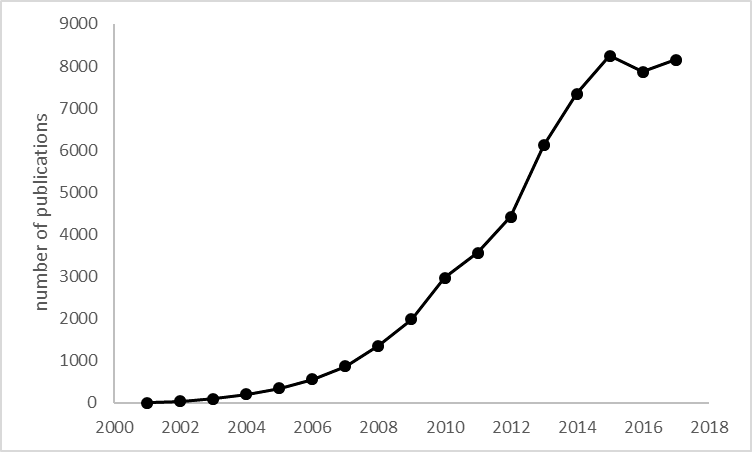
\includegraphics[width=1\textwidth]{ART_Kawalec/Kawalec-img001bw.png}
	\caption{The annual growth of publication number on microRNAs. Source: own analysis of MEDLINE dataset for ``microRNAs'', as MeSH keyword.}\label{fig1kawalec}
\end{figure}



\section{Particularist predilection of scientometric measures of science dynamics}
Despite divergence between the initial de Solla Price',s micro (logistic curve) and Kuhn',s macro (theory of paradigms) perspectives on science dynamics
%\label{ref:RNDSPq9qFoV4e}(Shapin, 2015)
\parencite[][]{shapin_kuhns_2015} %
 they merged adopting the latter',s particularist view. Kuhn in his 1969 \textit{Postscript} to \textit{The Structure of Scientific Revolutions}, originally published in 1962, defines ``paradigm'', by reference to scientific community: ``A paradigm is what the members of a scientific community share'', 
%\label{ref:RNDmOpL7aSSlG}(Kuhn, 1970, p.176).
\parencite[][p.176]{kuhn_structure_1970}. %
 One way to avoid vicious circularity in this characterization that Kuhn considers is by providing an independent identification of scientific communities, a task he would gladly relegate to sociologists and historians of science. In referring to ``preliminary results'', on this path he explicitly refers to publications concerning citation patterns of Dereck J. de Solla Price and Eugene Garfield, the two founding fathers of scientometrics 
%\label{ref:RNDQu3nw8129W}(Kuhn, 1970, p.178 n.6).
\parencite[][p.178 n.6]{kuhn_structure_1970}. %
 Kuhn',s ``naturalistic'', approach to science was subsequently ``enthusiastically incorporated'', into social-constructivist work \textit{via} the ``strong programme'', of Barry Barnes and David Bloor 
%\label{ref:RNDj43g7EUSjc}(Shapin, 2015).
\parencite[][]{shapin_kuhns_2015}. %
 Steve Fuller 
%\label{ref:RNDsh9a8sO9xR}(Fuller, 1992, p.270 n.107)
\parencite[][p.270 n.107]{fuller_being_1992} %
 notes a more direct connection between Kuhn and Price: ``the Kuhnian life cycle [of old paradigm-anomalies-crisis-revolution-new paradigm] is ‘Price',s Index,', which measures the obsolescence rate of journal articles in terms of diminishing citation patterns. A rapid obsolescence rate means a rapidly advancing research front, a paradigm at top puzzle-solving performance levels'',.\footnote{For a more detailed exposition of ``Price',s index'',,see 
%\label{ref:RNDvugEcFboHB}(De Mey, 1982, pp.148–170).
\parencite[][pp.148–170]{de_mey_cognitive_1982}.%
}

Fuller, commenting on the affinity between Kuhn',s and Price',s theories of science dynamics, observes that it strongly affected how scientometricians designed ``quantitative measures for tracking the growth of knowledge'', in view of ``science policy concerns'',. This approach is marked by characteristically particularist focus: ``[...] the major ‘product', of science is presumed to be the journal article, whose value is measured in terms of the other articles that cite it as instrumental in their own production. What makes today',s science so ‘big,', then, is the number of articles produced, and especially the exponential rate at which they are being produced. [...] Price seems to be impressed with the fact that out of a myriad of national interests can emerge a global picture of science that is reducible to fairly simple and intuitive logistic curves [...]'',
%\label{ref:RND7zMstr1jqu}(Fuller, 1992, pp.270–271).
\parencite[][pp.270–271]{fuller_being_1992}. %
 The overall dynamics of science, thus, results from aggregating individual publications and their co-citation patterns. It, therefore, explains why the particularist predilection has become a predominant view in various approaches in theory of science. In the following section I argue that this kind of particularistic approach is too simplistic and the overall dynamics results from an interaction of different kinds of processes 
%\label{ref:RNDYsXpqqPa9M}(Kawalec, 2020),
\parencite[][]{giovagnoli_cognitive_2020}, %
 the understanding of which preconditions our grasp of the dynamics of science.

\section{Processualist account of microRNAs discovery }
Particularist accounts of scientific progress face a number of challenges
%\label{ref:RNDbiB7GpylJ2}(Losee, 2004).
\parencite[][]{losee_theories_2004}. %
 Let me focus on two general ones, pertaining to the case of microRNAs. The first general problem, referred to here as \textit{the} \textit{granularity problem}, is concerned with the appropriate identification of the game-changer. The possibilities range here from a single publication, such as Copernicus',s \textit{De Revolutionibus} or Newton',s \textit{Principia}, to an extended period covering 300 years, as argued by Rupert Hall in his monumental \textit{The Scientific Revolution: 1500–1800} 
%\label{ref:RNDgseuFzcmxg}(Hall, 1954).
\parencite[][]{hall_scientific_1954}. %
 textitHall',s idea is that while prior to 1500 there was no scientific research characteristic of modern science, combining experimentation with mathematical language, it had been definitely established by the beginning of the 19\textsuperscript{th} century. Perhaps, none of the individual contributions, such as Copernicus',s or Newton',s, were sufficient to establish the practice of modern science as understood by Hall. However, the rounded dates disguise the apparent continuity with both, the prior and subsequent research. On the other hand, the individual publications are not comprehensible without reference to previous accomplishments, such as Ptolemy',s astronomy or Kepler',s laws, respectively. Hence, the task to isolate a particular research process as the moment of revolutionary or breakthrough change, seems rather hopeless.

Nevertheless, even if we suppose that such a precise and unproblematic identification would be possible, it encounters another problem, referred to here as \textit{the reference class problem}. A particular discovery or publication may be perceived as revolutionary from the perspective of quite different points of view, taking into account different antecedent and subsequent accomplishments. One example is Lavoisier',s chemical revolution
%\label{ref:RND86PBbivVjI}(Losee, 2004, p.66).
\parencite[][p.66]{losee_theories_2004}. %
 On one reading it constituted the culmination of a ``Stahlian revolution'', which ``emancipated chemistry from the domination of physics'',. Hence, against this background, it would be best understood in opposition to the Newtonian theory which claimed that matter comprises homogeneous particles by demonstrating the existence of qualitatively distinct chemical elements. Alternatively, Lavoisier',s work is seen as a preliminary stage culminating in the subsequent works of Dalton who was able to assign relative atomic weights to elementary species. Thus, a change of the reference class would result in a corresponding change in the particularist identification of the bearer of scientific revolution.

These problems indicate a need for an alternative account of scientific progress. So, let us now turn to one such alternative, namely the processualist standpoint. This brings us back to section 2, but now I will try to provide the processualist description of the early stages of the development of microRNAs as a new \textit{research routine}. The concept of research routine has been recently proposed as an alternative to traditional perspectives on research dynamics, which isolate its cognitive or social/institutional aspects and are confined to a particular area, such as philosophy, social studies of science or scientometrics. Research routine as a repeated and recognizable pattern of research practices of a scientific community (within Merton',s ``invisible college'',) sharing a symbolic representation (such as concept, classification, model or theory) integrates cognitive and institutional network dynamics of research processes, as exemplified by the examination of microRNAs research in
%\label{ref:RNDZPMNWLPU8u}(Kawalec, 2018).
\parencite[][]{kawalec_transformations_2018}. %
 In the next section, I identify two kinds of mechanisms underlying the dynamics of the microRNAs research routine.

On the wide-spread view of the history of molecular biology the identification of the structure and function of the double helix of DNA in 1953 set the stage for the subsequent development of molecular biology as a separate discipline. However, this view is not historically adequate as it downplays the role of the antecedent research on proteins and subsequent intense research concerning the role of RNAs that intermediated between DNA and proteins
%\label{ref:RNDBfvnn35yrA}(García-Sancho, 2012).
\parencite[][]{garcia-sancho_biology_2012}.%
\footnote{I am grateful to one of the Reviewers for stressing this point.} As. J. Darnell succinctly puts it: ``The bold discovery by James Watson and Francis Crick of the structure of DNA, often told, and well told, by the protagonists themselves, is frequently recited as the ‘start', of molecular biology. And if one watershed discovery is to be chosen as the ‘beginning,', that discovery is it. But there was a preceding half-century struggle of genetics and physical biochemistry [...]'', 
%\label{ref:RNDe6bPAtwv5V}(Darnell, 2011, p.2).
\parencite[][p.2]{darnell_rna_2011}. %
 The period 1950–1980 that followed recognized ``the centrality of RNA to life'', due to plentiful discoveries of the types of RNA molecules and their specific functions (esp. tRNA, ribosomes, mRNA, pre-mRNA, pre-rRNA, RNA splicing, etc.). This process of gradual realization of the importance of RNA is well epitomized by the \textit{RNA world} hypothesis concerning the initial phase in the evolution of life. The detailed account of research advancements concerning RNA in the period of 1953–1980 by Darnell 
%\label{ref:RNDpzNwn6PmtN}(2011)
\parencite*[][]{darnell_rna_2011} %
 undermines the widespread particularist focus on the discovery of the double helix as the sole ``start'', of molecular biology.

Of course, the discovery of microRNAs as noncoding small RNAs is entrenched in these conceptual advances in RNA investigations that began in 1953. The laboratory practices that made this discovery possible include Syndey Brenner',s work on the genetics of \textit{C. elegans} in the late 1960',s and early 1970',s that established this nematode as the model organism for genetic studies. Robert Horvitz and his collaborators by 1980 identified cell lineages for \textit{C. elegans} and its mutant forms (24 in total), including two ``heterochronic'', genes \textit{lin-4} (short from ``lineage abnormal'',) and \textit{let-7} (``lethal'',). Further, Horvitz and his post-docs, Ambros and Ruvkun, in the late 1980s were able to identify the functional model specifying interdependence between heterochronic genes in \textit{C. elegans}, focusing on the relation between \textit{lin-4} and \textit{lin-14}. The famous paper
%\label{ref:RNDM85sa5wRCR}(Lee, Feinbaum and Ambros, 1993)
\parencite[][]{lee_c_1993} %
 provided the details of the molecular model of the regulatory mechanism between the two genes. These accomplishments were accompanied by a flow of changes in experimental techniques 
%\label{ref:RNDpIrYhbF31B}(Kawalec, 2020).
\parencite[][]{giovagnoli_cognitive_2020}. %
 Further research on \textit{C. elegans} resulted in the discovery of RNA interference (RNAi) in 1998. Soon thereafter, Ruvkun and his collaborators identified the second microRNA, namely \textit{let-7} and demonstrated its high evolutionary conservation. Several laboratories instantly joined in, including Tom Tuschl',s and David Bartel',s searching for new microRNAs both in \textit{C. elegans} as well as in other organisms. These early findings were jointly reported in 2001 in \textit{Science} 
%\label{ref:RNDIa8ZxSmJSb}(Lagos-Quintana et al., 2001; Lau et al., 2001; Lee and Ambros, 2001).
\parencites[][]{lagos-quintana_identification_2001}[][]{lau_abundant_2001}[][]{lee_extensive_2001}. %
 A new line of research was initiated by the team led by George Calin who first documented a relation between oncogenesis and deletion or down-regulation of microRNAs as early as 2002. Subsequent research on microRNAs included, for instance, prediction of targets, biogenesis, identification of microRNAs in different organisms, diagnostic and therapeutic potential, occurrence in body fluids and identification of other noncoding RNA particles. It has ``revealed that miRNAs play important roles in diverse processes such as cell differentiation, cell proliferation, and organ development. More importantly, beyond their roles in physiological processes, extensive research has explored miRNA involvement in various pathologies, including infectious diseases'', 
%\label{ref:RNDAMNvOo87Va}(Fu et al., 2011, p.4246).
\parencite[][p.4246]{fu_circulating_2011}. %
 The end of the early phase in development of microRNAs research routine is marked by 2006 when the next-generation sequencing methods enabled more efficient research.\footnote{For a systematic exposition of the phases in microRNAs research, see 
%\label{ref:RNDhrMaHpUTcC}(Kawalec, 2018).
\parencite[][]{kawalec_transformations_2018}. %
 In private communication this account has been approved by Victor Ambros and Robert Horvitz.}

Without going too much into the details, let me give a perspicuous illustration of the processual nature of the discovery of microRNAs. The initial discovery of the molecular regulatory mechanism between \textit{lin-4} and \textit{lin-14} in 1993 was initially perceived as a phenomenon specific to \textit{C. elegans} and, perhaps, related nematodes. It was only the subsequent discoveries of the universal RNAi mechanism in 1998 and the second microRNA \textit{let-7} with its high evolutionary conservation in 2000 that eventually established a new taxonomic category of ``microRNAs'', in 2001. So, the two publications that appeared in 1993 only with this hindsight can be retrospectively recognized ``a breakthrough'',. The pressing question to proponents of particularism would now be: When the discovery of microRNAs actually took place? Was it just 1993,\footnote{Note that the main results were actually known earlier, but intentionally withheld from publication for several months.} or the whole 8-year period?, or, perhaps, an even longer one, if one would like to consider more recently discovered ``oncoMIRs'', or ``circulating microRNAs'',?

\section{Varied mechanisms of science dynamics: the fate of \textit{lin-4} and \textit{let-7}}
In the preceding section I indicated the granularity and reference class problems as the reasons why the particularist view of the dynamics of microRNAs, as depicted on Figure \ref{fig1kawalec}, may be misleading. Yet, there is another reason why this may be so. The simplistic pronouncements of particularists may turn our attention away from the complexity of the mechanisms underlying the dynamics. In this section I will provide a detailed illustration of such a complexity as exemplified by two research sub-routines concerning the first two microRNAs discovered, namely \textit{lin-4} and \textit{let-7}.

One way to grasp the overall dynamics of microRNAs routine is to observe how the entire network, such as co-authorship of publications, develops. The tools provided by network analysis allow one to trace how ``the invisible college'',
%\label{ref:RNDi5rOEY3AmT}(Merton and Garfield, 1986, pp.viii–ix)
\parencite[][pp.viii–ix]{merton_foreword_1986} %
 develops with a new routine. An important indicator of this dynamics is ``the giant component'', of a given network that forms the largest set within the network of authors who are ``connected'', by their collaboration. In case of an emerging routine the whole network is dispersed and the giant component is hardly distinguishable from other groups of connected papers. In other words, there is no clear indication of a dominance of a particular group of authors. And, to use Merton',s wording, it could be interpreted as a stage where no invisible college can be clearly identified.

In contrast, mature routine is characterized by the clearly present, and dominant, giant component. Usually, the critical point is 50\% of all nodes, such as authors, in the given network. Figure \ref{fig2kawalec} contrasts two stages of the development of the author network with links signifying co-authorship relations. The 1993 stage captures the early phase of microRNAs routine development with Horvitz as the leader of the ``giant'', component. However, at this stage, the routine is still in its infancy as the ``giant'', component embraces only 26 people, that is 11\% of all the authors. In 2018 the routine is apparently mature: while the giant component consists of 70\% of all the authors, their total number increased by an astonishing (almost) 100 times.

\begin{figure}[h!]
\begin{flushleft}
\tablefirsthead{}
\tablehead{}
\tabletail{}
\tablelasttail{}
\begin{tabular}{m{.5\linewidth}|m{.5\linewidth}}
{\centering\bfseries 1993\par}

 &
{\centering\bfseries 2018\par}

\\
 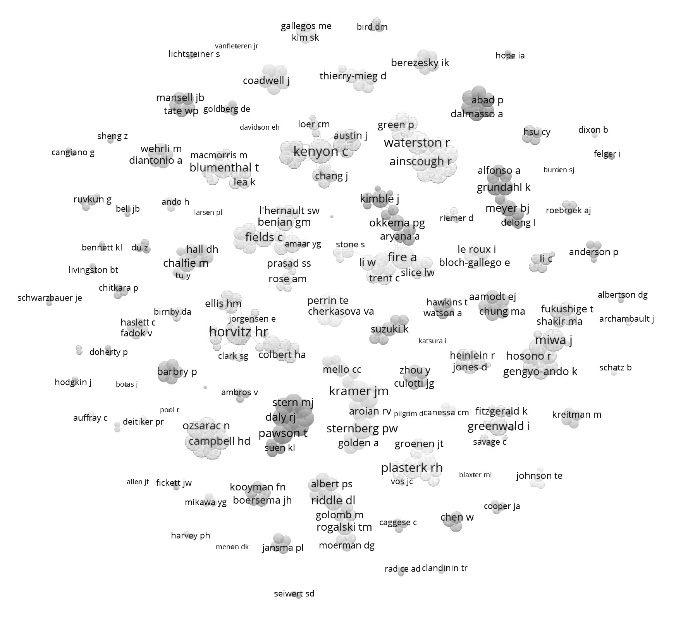
\includegraphics[width=.5\textwidth]{ART_Kawalec/Kawalec-img002bw.jpg}  &
 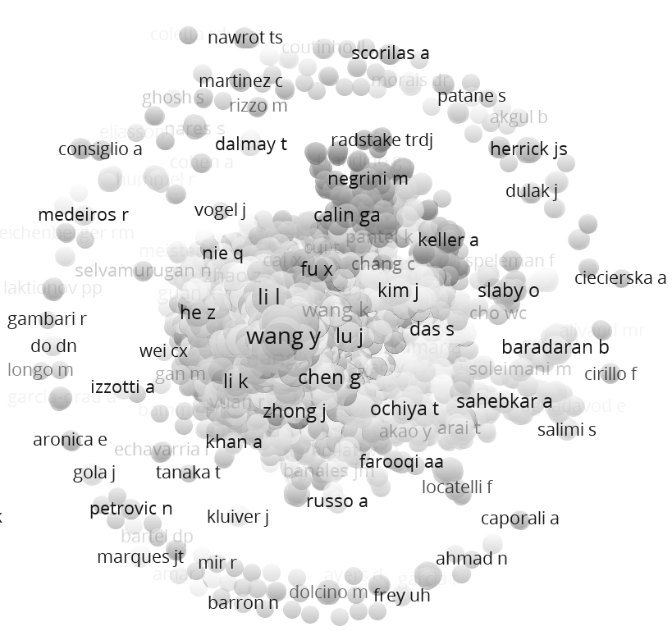
\includegraphics[width=.5\textwidth]{ART_Kawalec/Kawalec-img003bw.png} \\
\multicolumn{2}{c}{{\centering\bfseries giant component}
}\\
\centering 6\% (of 436 authors) &
\centering\arraybackslash 70\% (of 38 703 authors)\\
\end{tabular}
\end{flushleft}
\caption{Dynamics of microRNA routine – the expansion of size and the giant component of collaborating authors. Source: own analysis of MEDLINE dataset for “microRNAs” as keyword.}\label{fig2kawalec}
\end{figure}

It should be noted, however, that the dynamics between 1993 and 2018 is a very complex and multidimensional process. It cannot simply be captured, as claimed by proponents of particularism, by highlighting some important publications or dates, for it is a continuous process resulting from a set of interacting mechanisms. The discussion of \textit{lin-4} and \textit{let-7} in the remainder of this section illustrates just one aspect of this complexity.

The first microRNAs discovered in \textit{C. elegans lin}-4 and \textit{let}-7 were initially named ``small temporal'', (stRNAs) to emphasize the fact that they are developmentally regulated as well as they control developmental programs
%\label{ref:RNDxU5z6vTHLm}(Lagos-Quintana et al., 2002),
\parencite[][]{lagos-quintana_identification_2002}, %
 such as Dauer larva or vulva formation: ``\textit{lin}-4 and \textit{let}-7 control the timing of postembryonic events by translational repression of target genes, permitting progression from early to late developmental programs'', 
%\label{ref:RNDjC15tfAZXc}(Sempere et al., 2003, p.9).
\parencite[][p.9]{sempere_temporal_2003}. %
 While \textit{let-7} was early identified in a wide class of organisms, \textit{lin-4} was thought to be specific to worms. Early search for new microRNAs in mouse tissue led in 2002 to discovery of \textit{lin-4} ortholog miR-125 which is more widely present in other species, including humans 
%\label{ref:RNDtegoozSxYu}(Yin et al., 2015).
\parencite[][]{yin_progress_2015}. %


Apparently, another important difference between \textit{lin-4} and \textit{let-7} that was noted early on was the recognition of the role of \textit{let-7} in oncogenesis and tumor suppression. Hence, \textit{let-7} has become an object of intense studies as it ``was considered as the most important miRNA for the cancer incidence and progression'',
%\label{ref:RNDLaW8XsZykT}(Wang, Jiang and Xu, 2018).
\parencite[][]{wang_comprehensive_2018}. %
 The role of homologs of \textit{lin-4} in oncogenesis was noted later and was less apparent 
%\label{ref:RNDymkacnfBGk}(Sonoki et al., 2005).
\parencite[][]{sonoki_insertion_2005}. %
 The differences between \textit{lin-4} and \textit{let-7}, at least partly, explain the difference in their respective research dynamics as presented in figure \ref{fig3kawalec} which depicts the dynamics of topical expansion of both research lines against the annual growth of the number of publications.
\begin{figure}[h!]
	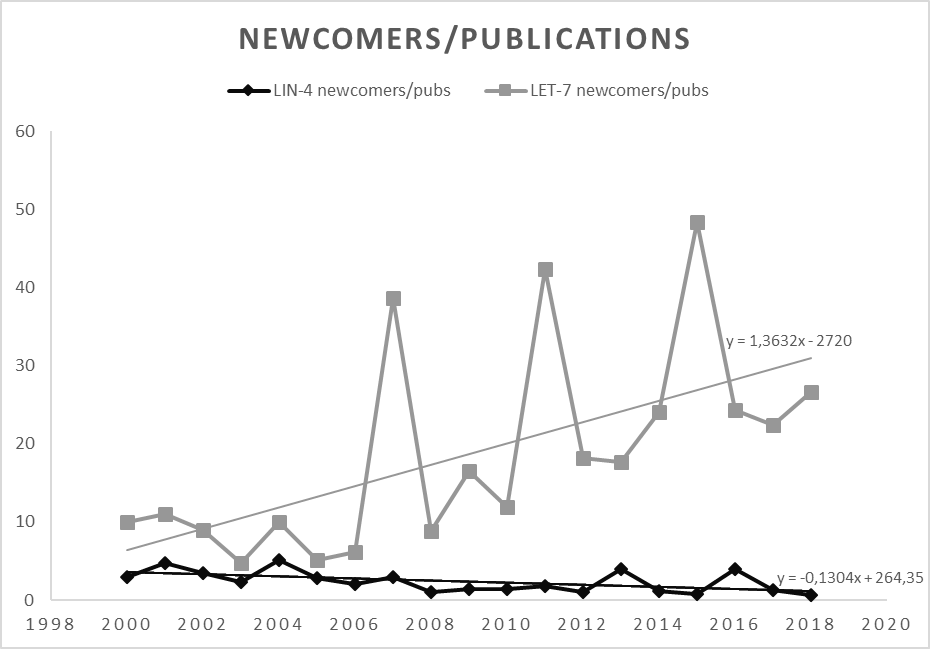
\includegraphics[width=1\textwidth]{ART_Kawalec/Kawalec-img004bw.png}
	\caption{Newcomer dynamics of MeSH keywords relative to the annual number of publications for the first two microRNAs: \textit{lin-4} and \textit{let-7}. Source: own analysis of MEDLINE datasets for ``\textit{lin-4}'', and ``\textit{let-7}'', as keywords, respectively. The number of hitherto unrecorded MeSH keywords (``newcomers'',) for a given year was measured against the annual publication record for ``\textit{lin-4}'', and ``\textit{let-7}'',,respectively. The trendlines were estimated as linear functions.}\label{fig3kawalec}
\end{figure}

Interestingly, both processes are characterized by peaks with \textit{let-7} displaying their stronger impact. Those peaks represent a sudden growth of interest in microRNAs and outbursts of hitherto unused MeSH keywords.\footnote{The MEDLINE classificatory scheme of MeSH keywords, in contrast to author keywords, provides a consistent measure of topical expansion of a given research area.} Elsewhere
%\label{ref:RNDMyMMlnwtOG}(Kawalec, 2020)
\parencite[][]{giovagnoli_cognitive_2020} %
 I provided an explanation of this phenomenon in terms of the underlying inherent mechanisms and unexpected external shocks. The account presented here, thus, is a modified processualism as it accommodates unexpected impulses independently from the inherent dynamics of a series of research processes, which are informed by the outcomes of the antecedent ones and, as claimed by D.J. de Solla Price, typically instantiate the logistic curve. The external shocks may be difficult to satisfactorily characterize as they presumably embrace a wide class of phenomena from new discoveries pertaining to microRNAs, through new research methods and instruments to new institutional arrangements, such as installment of new laboratories or funding schemes.

Nevertheless, in the presented case of \textit{let-7} some clues seem quite plausible. The initial discovery of the molecular regulatory mechanism of \textit{let-7} and its high evolutionary conservation
%\label{ref:RNDXszYukj7pQ}(Nelson and Ambros, 2019)
\parencite[][]{nelson_trans-splicing_2019} %
 drew attention of several important research laboratories, such as Bartel',s or Tuschl',s and resulted in 2001 in a first wave of new microRNAs discoveries, both in \textit{C. elegans} and other organisms. The whole area of microRNAs research was strongly impacted by introduction around 2006 of new instruments of ``next-generation sequencing'', enabling high-throughput analysis. This was reflected in a subsequent proliferation of topics that peaked in 2007, including identification of \textit{let-7} targets, such as the gene \textit{Hmga2} (\textit{High Mobility Group A2}) having being already well-known for its expression ``in a wide variety of benign and malignant tumors'', 
%\label{ref:RNDHB1OgkqYEs}(Mayr, Hemann and Bartel, 2007, p.1576).
\parencite[][p.1576]{mayr_disrupting_2007}. %
 Demonstrating thus the high diagnostic and therapeutic potential of \textit{let-7} 
%\label{ref:RNDqoFLg9dZgk}(Johnson et al., 2007; Kuehbacher et al., 2007; Park et al., 2007; Cinkornpumin et al., 2017; Pobezinsky and Wells, 2018; Roos et al., 2018).
\parencites[][]{johnson_let-7_2007}[][]{kuehbacher_role_2007}[][]{park_let-7_2007}[][]{cinkornpumin_small_2017}[][]{pobezinsky_lets_2018}[][]{roos_pharmacologic_2018}. %
 Later, the role of \textit{let-7} was recognized in post-transcriptional control of innate immune responses to pathogenic agents and allergic inflammation linking this microRNA to adaptive immunity 
%\label{ref:RNDUAP1ignAmN}(Schulte et al., 2011; Kumar et al., 2011).
\parencites[][]{schulte_analysis_2011}[][]{kumar_let-7_2011}. %
 Finally, the year 2015 marks an intense exploitation of the therapeutic and diagnostic potential of the circulating microRNAs that are present in bodily fluids and therefore have good potential as an accessible and attractive biomarker.

\section{Concluding remarks}
As demonstrated in figure \ref{fig3kawalec}, although the interest in \textit{lin-4} is slightly declining, like \textit{let-7} it still remains an object of a steady line of research that brings about new insights. The mechanism of developmental timing pathway of \textit{lin-4} and \textit{let-7} as the first ``small temporal'', or ``heterochronic'', regulatory genes appears to be quite universal
%\label{ref:RND1PazrnVE9B}(Bracht et al., 2010).
\parencite[][]{bracht_regulation_2010}. %
 On the other hand, however, \textit{let-7} is apparently more prone to external shocks. It, at least partly, derives from its high therapeutic and diagnostic potential. Thus, we have a clear illustration of both general problems of particularism discussed in the previous section. An attempt to pin down the milestones in the development of research on \textit{let-7} may be quite misled by the external shocks that strongly affect the tangible dynamics of this line of research.

Consider now the reference class problem. The often made claim that Ambros and his collaborators discovered microRNA in 1993 is obviously a short-cut. To appreciate the general nature of the non-coding mechanism of \textit{lin-4} the discovery of \textit{let-7} was needed. Moreover, several other discoveries were needed to reveal microRNAs',s biogenesis, their targets, different forms in different organisms, role in developmental and pathogenic processes, etc. Hence, if -- following the particularist practice -- we would single out the 1993 paper by Ambros and collaborators as the source of the breakthrough this will leave us with a very simplistic notion of ``microRNA'',. Similarly, an alternative way to pin down the discovery with regard to the combination of the two 1993 papers by Ambros',s and Ruvkun',s teams and the latter',s two 2000 papers would face similar problems. On the other hand, focusing on -- all, or one, of -- the most spectacular peaks in the dynamics of \textit{let-7} may misguide the real cognitive mechanism and turn us, instead, to the external shocks.

Particularist atttempts to pin down the moment of discovery, or its most important outcome, may have an important social role, such as prestigious awards, policy decision-making or public communication of science. Nevertheless, the integrative explanation of the dynamics would need to acknowledge the complexity of the whole process of discovery.

\section{Acknowledgments }
An earlier version of this paper was presented on January 21 in 2019 at the PAU Commission on the Philosophy of Science. I appreciate the comments received during the discussion that helped me to improve the final draft.

I am grateful to the anonymous Reviewers for their constructive comments and insightful recommendations which helped to improve the quality of the paper.

\end{artengenv} %bw-col

\begin{artengenv}{Szymon Czarnik}
	{How much truth is in stereotypes?}
	{How much truth is in stereotypes?}
	{How much truth is in stereotypes?}
	{Institute of Sociology, Jagiellonian University}
	{Stereotype accuracy is a contentious topic. Part of the problem is that typically stereotypes are generic statements whose truth status is unclear due to the fact that they are ill-defined quantitatively. The article focuses on the epistemic aspect of stereotypical beliefs. In the ongoing debate, I side with those who argue against stereotypes being wrong or inaccurate by virtue of definition alone. I propose that, when possible, stereotype accuracy should be assessed in probabilistic terms by inspecting how likely a generic statement is to be true when applied to individual(s) representative of the relevant group(s). This approach applies equally well to investigating the actual and the perceived accuracy of stereotypes.}
	{stereotypes, stereotype accuracy, epistemology, probabilistic approach.}

\vspace{2\baselineskip}
\lettrine[loversize=0.13,lines=2,lraise=-0.05,nindent=0em,findent=0.2pt]%
{I}{}n this paper, I propose that stereotypes are best understood as generic statements whose truth status is unclear. They are expressed by asserting that ``members of group A have trait T,'' or ``Members of group A are higher/lower on trait T than members of group B.'' Such utterances lack proper quantification and invite alternative interpretations. One such interpretation is that stereotypes speak of all group members without exception which leads to the idea that stereotypes should be considered false by definition, which in turn leads to the opposition to stereotype accuracy research as, at best, a misguided endeavor. This opposition, however, is unfounded on epistemic grounds once we explicitly recognize generic nature of stereotypes. Thus after outlining the long-lasting debate, I proceed to discuss the problems inherent in measuring the accuracy of stereotypes, and then advocate a probabilistic approach, i.e. assessment of probabilities that individuals conform to the generic rule posited by a stereotype. As a practical illustration, I show a number of such probabilistic assessments based on data from representative samples. Finally, I propose that the very same probabilistic approach should be used to directly investigate how accurate people perceive their own stereotypes to be. This in turn would provide an easy and straightforward method of comparing perceived and actual accuracy of stereotypes, acknowledging a possibility that stereotypical perceptions may both over- and underestimate actual differences.


\begin{center}
$ {\ast}\,{\ast}\,{\ast} $
\end{center}


A scholarly dispute over stereotypes is to no small extent a semantic issue. The problem is that a typical stereotype assumes a form of what \textit{The Stanford Encyclopedia of Philosophy} calls a generic, i.e. a statement which expresses a generalization ``but unlike quantified statements, [...] do[es] not carry information about how many members of the kind or category have the property''
%\label{ref:RNDGhTTUrWVcB}(Leslie and Lerner, 2016).
\parencite[][]{leslie_generic_2016}. %
 ``Some men are taller than some women'' is certainly a true statement. Equally certainly, ``All men are taller than all women'' is a false statement. But the case is that when you hear anybody compare the height of men and women, it will be in the form of a generic ``Men are taller than women.'' A quantitative indeterminacy of such an utterance will either be construed to be vaguely true and will be silently approved, or will invite a dispute and be contested.

\enlargethispage{.7\baselineskip}
In daily life conversations, calling somebody's remark a stereotype is surely a form of criticism. In common parlance, as well as in vast sociological and psychological literature, the term ‘stereotype' implies untruth, or inaccuracy of the assertion. A general statement like ``Scots are cheap'' may be picked apart as untrue in the sense that on average Scots are no more stingy than members of any other ethnic group. Or, even if the statement had some kernel of truth in it, one could be brought to task for inaccurately applying it to pass a judgment on a particular individual who may happen not to conform to this general rule.\footnote{Far from being limited to stereotypical beliefs, the problem of group-to-individual generalizability may pose a serious threat to scientific research involving human subjects
%\label{ref:RNDTlfuAJ4ACM}(Fisher, Medaglia and Jeronimus, 2018).
\parencite[][]{fisher_lack_2018}.%
} Apart from being misguided epistemologically, the utterance may also be criticized on moral grounds as an attempt at a wholesale vilification of a certain group of people. Thus the presumed wrongness of stereotypes may consist in epistemic and/or moral failure 
%\label{ref:RNDo2Xq32gcjA}(Beeghly, 2014).
\parencite[][]{beeghly_seeing_2014}. %
 It is solely the former aspect of stereotypes that we shall be concerned with here.\footnote{Some authors reduce stereotypes to the epistemic aspect alone. Thus Banaji claims that ``[f]rom the earliest use of the term in psychology, stereotypes have been regarded as the cognitive (thought) as opposed to the affective (feeling) component of mental representations of social groups. As such, the construct is tied to but differentiated from the concept of attitude, preference, or liking as well as the concept of discrimination'' 
%\label{ref:RNDHS9MlJPRnC}(Banaji, 2001, p.15101).
\parencite[][p.15101]{banaji_stereotypes_2001}. %
 }

\section{Resistance to research on stereotype accuracy}
Before we proceed further it should be acknowledged that, for a good reason, the ethical aspect looms large in the scholarly literature on the topic. In psychology, stereotypes are studied as cognitive components of prejudice, which may be brought about by and contribute to inter-group hostility
%\label{ref:RND4lT4IExI0w}(Bar-Tal, 1989);
\parencite[][]{bar-tal_delegitimization_1989}; %
 in sociology, they are recognized as a device that may adversely affect targeted groups by means of self-fulfilling prophecy 
%\label{ref:RNDq8zLOYvax2}(Merton, 1948);
\parencite[][]{merton_self-fulfilling_1948}; %
 in criminology, they are discussed in the context of racial/ethnic profiling in police operations 
%\label{ref:RNDFHF118jk89}(Schauer, 2003);
\parencite[][]{schauer_profiles_2003}; %
 in historical studies, they are investigated as part and parcel of totalitarian propaganda 
%\label{ref:RND3zPpNfYi3y}(Werth, 2011; USHMM (United States Holocaust Memorial Museum),
\parencites[][]{werth_dekulakisation_2011}[][]{ushmm_united_states_holocaust_memorial_museum_defining_nodate}%
; in economics, they are incorporated in models of statistical discrimination in the labor market 
%\label{ref:RNDgoefvun65q}(Arrow, 1971; Phelps, 1972).
\parencites[][]{arrow_theory_1971}[][]{phelps_statistical_1972}. %
 It goes without saying that after Adorno had linked stereotypic thinking with fascist belief systems the concept became even more anathema 
%\label{ref:RNDHdzxZxrjhG}(Jones and Colman, 2001).
\parencite[][]{jones_stereotypes_2001}.%


It is then easy to see why the very idea of considering stereotype accuracy has been frowned upon. Being a lively research field until around mid-1950s, in later years accuracy research nearly ceased to exist
%\label{ref:RNDEUrLdTnpLb}(Jussim, 2012).
\parencite[][]{jussim_social_2012}. %
 Recognized harmful implications of stereotypes made most researchers extremely reluctant to lend them any credibility for fear of promoting any sort of prejudice. In most of the writings on stereotypes, this reluctance tended to be implicitly transformed into a non-sequitur assumption that ``if stereotypes are associated with social wrongs, they must be factually wrong'' 
%\label{ref:RNDbpqmbn3un6}(Jussim et al., 2009, p.199).
\parencite[][p.199]{jussim_unbearable_2009}. %
 This conflation was brought up and chastised as early as 1965 by Roger Brown who opined that it was a disingenuous device by means of which the social psychologist ``perverted his science to achieve a moral purpose'' 
%\label{ref:RND5F22AusjVZ}(Stroebe and Insko, 1989, p.5).
\parencite[][p.5]{stroebe_stereotype_1989}.%
\footnote{We encounter a similar sentiment even earlier in a seminal book 
%\label{ref:RND0GRWHWvKN6}(Allport, 1954, p.87):
\parencite[][p.87]{allport_nature_1954}: %
 ``we find social scientists who overhastily reject the very possibility of racial, national, or group differences of any appreciable or fundamental order. Some of them do so on the basis of charitable motives, but the evidence they offer is usually fragmentary''. He even goes as far as to urge researchers to investigate ``all the facts we can get to evaluate the alleged claim that a hated group merits hostility—that its evil reputation is well deserved'' 
%\label{ref:RNDVZBwqFCsZG}(Allport, 1954, p.104)
\parencite[][p.104]{allport_nature_1954}%
—an utterance that in the present day and age would likely bring upon him a charge of ``blaming the victim''. } Still thirty years later, going against the tide, the editors of \textit{Stereotype Accuracy. Toward Appreciating Group Differences} forewarned in the preface:

\myquote{
It is not easy to do research on stereotype accuracy, for both scientific and political reasons […]. The intellectual content of this book commits multiple heresies […] the idea that stereotypes may sometimes have some degree of accuracy is apparently anathema to many social scientists and laypeople. Those who document accuracy run the risk of being seen as racists, sexists, or worse
%\label{ref:RNDt9JkRYIBWn}(Lee, Jussim and McCauley, 1995, p.xiii).
\parencite[][p.xiii]{lee_stereotype_1995}.%
\footnote{Indeed, stereotypes acquired such a contemptible connotation that it became a useful strategy for overbearing intellectuals to attach the term to any commonsensical statement they found unpalatable. As Thomas Sowell observed, ``the very conception of testing beliefs against reality is attacked by such things as deconstruction, cultural relativism, and the practice of describing uncongenial conclusions as ‘perceptions' or ‘stereotypes' and attributing ‘false consciousness' to those who hold them'' 
%\label{ref:RNDjeSrl3zJq4}(Sowell, 1995, p.244).
\parencite[][p.244]{sowell_vision_1995}. %
 }
}


Needless to say, authors go to great lengths to explicate why the slur is utterly unfounded.

\section{Ambiguity about truth status of stereotypes}
Hostility toward stereotype accuracy reported by Jussim et al. notwithstanding, one should recognize that from the very outset there was a lot of ambiguity about the truth status of stereotypes. Two of the most seminal pieces on stereotypes, viz. Part III of \textit{Public Opinion} by Walter Lippmann (credited with introducing the concept in 1922), and \textit{The Nature of Prejudice}
%\label{ref:RNDZbhHfsclbw}(1954)
by Gordon W. Allport
\parencite*[][]{allport_nature_1954} %
are case in point. They both consider stereotype formation as a natural and inevitable process taking place in human mind when people try to make sense of a limited amount of information. Likewise, they both admit that beliefs about groups may be correct to different degrees. Thus, for example, Lippmann 
%\label{ref:RNDBg29dJm9cU}(1998, p.90)
\parencite*[][p.90]{lippmann_public_1998} %
 observes:

%\enlargethispage{1\baselineskip}
\myquote{
Were there no practical uniformities in the environment, there would be no economy and only error in the human habit of accepting foresight for sight.\footnote{Lippmann construed stereotypes as preconceptions that guide and organize our perception. } But there are uniformities sufficiently accurate, and the need of economizing attention is so inevitable, that the abandonment of all stereotypes for a wholly innocent approach to experience would impoverish human life.
}

But having admitted this much, he offers a very telling example of what he considers to be a perfect stereotype. He invokes Aristotle's infamous defense of slavery in Book I of \textit{Politics}. Therein the philosopher instructs his readers that nature created the bodies of slaves and free men different from each other: the former fit for servile labor, the latter for civil life. Utter nonsense as it is, notes Lippmann, training Greeks to see slaves as slaves by nature was presumably the only ``righteous'' justification of the institution one could offer. He then sums up Aristotle's persuasion strategy:

\myquote{
Each slave holder was to look upon his chattels as natural slaves. When his eye had been trained to see them that way, he was to note as confirmation of their servile character the fact that they performed servile work, that they were competent to do servile work, and that they had the muscles to do servile work.

This is the perfect stereotype. Its hallmark is that it precedes the use of reason; is a form of perception, imposes a certain character on the data of our senses before the data reach the intelligence […]. There is nothing so obdurate to education or to criticism as the stereotype. (p.98)
}

In a similar fashion Allport
%\label{ref:RNDoannRVTDJI}(1954, pp.189–190),
\parencite*[][pp.189–190]{allport_nature_1954}, %
 while conceding that some stereotypes ``need not be altogether false'', points to the fact that there are as well some that ``are totally unsupported by facts'' and it's possible for them ``to grow in defiance of all evidence.''

%\enlargethispage{1\baselineskip}
\section{Are stereotypes untrue by definition?}
There is not one agreed upon definition of stereotypes. Probably the shortest and most general definition of stereotypes as ``category-based knowledge'' was provided \textit{en passant} by Macrae and Quadflieg in a chapter on perceiving people
%\label{ref:RND3OKSCJItmJ}(Macrae and Quadflieg, 2010, p.428).
\parencite[][p.428]{macrae_perceiving_2010}. %
 In the social context, such categories would predominantly be groups of people sharing a certain salient characteristic. Naturally enough, most definitions add certain qualifications, of which the one pertinent to our topic is whether stereotypes are necessarily untrue, or inaccurate. As Stroebe and Insko 
%\label{ref:RNDBPlnl0NzfU}(1989)
\parencite*[][]{stroebe_stereotype_1989} %
 point out, stereotypes have often been defined as ``incorrect generalizations''; they were variously meant to be ``relatively unresponsive to external reality'' 
%\label{ref:RNDg8YZLD95aE}(Klineberg, 1951),
\parencite[][]{klineberg_scientific_1951}, %
 ``exaggerated'' 
%\label{ref:RNDik6HuiuzNF}(Allport, 1954),
\parencite[][]{allport_nature_1954}, %
 ``biased'' 
%\label{ref:RNDf006k8PUql}(English and English, 1958),
\parencite[][]{english_comprehensive_1958}, %
 ``generally invalid'' 
%\label{ref:RNDI3CYnMSqCL}(Miller and Turnbull, 1986)
\parencite[][]{miller_expectancies_1986}%
\footnote{It is ironic and telling that defining stereotypes as generally invalid, Miller and Turnbull quote Ashmore and Del Boca 
%\label{ref:RNDP7GpDYrS3x}(1981)
\parencite*[][]{hamilton_conceptual_1981} %
 who, in the very paper quoted, explicitly advocated accuracy-neutral definition: ``Stereotypes have been defined as ‘bad' for one or a combination of the following reasons: A stereotype is a set of beliefs that is incorrectly learned, overgeneralized, factually incorrect, or rigid [...]. While stereotypes may well have any or all of these characteristics, the proposed sources of ‘badness' should not be incorporated into the definition of the term ‘stereotype''' 
%\label{ref:RNDKNEzt09O1t}(Miller and Turnbull, 1986, p.16).
\parencite[][p.16]{miller_expectancies_1986}.%
}, ``oversimplified'' 
%\label{ref:RNDIW40zgJp1x}(Koleser, 2008),
\parencite[][]{koleser_stereotyping_2008}, %
 ``over-generalized'' 
%\label{ref:RNDgh0MDtr3mm}(Wikipedia, 2020),
\parencite[][]{wikipedia_stereotype_2020}, %
 etc.\footnote{Other characteristics, frequently added, have rendered stereotypes negative, resistant to change, and disindividualized (shared within a particular social environment).} However, Jussim et al. 
%\label{ref:RNDWPSqDkaPbN}(2009)
\enlargethispage{-.5\baselineskip}%
\parencite*[][]{jussim_unbearable_2009} %
 supplied a cogent argument against such defining away of stereotype's accuracy. The argument is two-fold as, logically, there are only two possible interpretations of the assertion that all stereotypes are inaccurate. First reading is that all beliefs about groups are stereotypes and they are all wrong. As a matter of fact, hardly anybody subscribes to such a claim. It is quite obviously self-defeating because if it was true, any meaningful discussion about groups of people would \textit{ipso facto} be impossible. Second interpretation is that not all beliefs about groups are wrong and we call stereotypes only those that are.\footnote{This in fact was the position taken by Allport who made an explicit distinction between stereotypes (distorted beliefs) and group traits (real differences between groups): ``If [an image of a category] is a generalized judgment based on a certain probability that an object of the class will possess a given attribute, we would not call the judgment a stereotype'' 
%\label{ref:RNDdBClyv6yLF}(Allport, 1954, p.189).
\parencite[][p.189]{allport_nature_1954}. %
 And then: ``We can distinguish between a valid generalization and a stereotype only if we have solid data concerning the existence of (the probability of) true group differences'' 
%\label{ref:RNDyBG6R329S4}(Allport, 1954, p.192})
\parencite[][p.192]{allport_nature_1954}.}
 The problem with this approach is that it is inconsistent with the actual practice of research on stereotypes. It necessitates that the first step in stereotype research should be to demonstrate that the belief under investigation is indeed factually wrong. Otherwise, it would plainly not be a stereotype study. However, in practice that first step is typically skipped, the burden of proof is left untouched and it is simply assumed that the belief is false.\footnote{The reason for this
% , Jussim et al. 
%\label{ref:RNDnGvl9HW20z}(2016, p.33)
%\parencite*[][p.33]{jussim_stereotype_2016} %
% surmise,
 is that ``social psychologists once so firmly believed in stereotype inaccuracy, that declaring stereotypes to be inaccurate did not even require a reference!'' \parencite[][p.33]{jussim_stereotype_2016}} Jussim et al. 
%\label{ref:RNDlkKeugSyNP}(2016, p.32)
\parencite*[][p.32]{jussim_stereotype_2016} %
 dub this phenomenon ``The Black Hole at the Bottom of Many Declarations of Stereotype Inaccuracy''. By means of exemplification, they quote a passage from a world-renowned social psychology handbook stating that ``[t]o stereotype is to allow those pictures [i.e. our mental images of external reality] to dominate our thinking, leading us to assign identical characteristics to any person in a group, regardless of the actual variation among members of that group'' 
%\label{ref:RNDfTxHUaw0Cl}(Aronson, 2011, p.309).
\parencite[][p.309]{aronson_social_2011}. %
 As they are quick to notice, Aronson ``does not cite anything to support such an extreme claim because he cannot. After nearly 100 years of empirical research on social stereotypes, there is not a single study that has reported a single person who believes all members of any group have identical characteristics'' 
%\label{ref:RND2AGqqANLO3}(Jussim et al., 2016, p.33).
\parencite[][p.33]{jussim_stereotype_2016}.%

\enlargethispage{.5\baselineskip}
Still another more serious problem is that stereotype itself is a categorical concept, and since beliefs about groups may be located anywhere on the continuum between blatant falsehood and clear truth, to categorize a statement as a stereotype one needs to choose a cut-off point—a purely arbitrary decision. To be sure, any academic might argue that the cut-off point should simply be 100\% true; that a given stereotype, e.g. that men are taller than women, may be considered true only if each and every man is taller than any woman.\footnote{As the above quote from Aronson shows, this line of reasoning is routinely employed to demonstrate that stereotypes are false. } But then one is left wondering how many of the propositions based on social-scientific studies would hold their ground for more than five seconds when faced with such an absurdly high standard of truth.\footnote{As a matter of fact, Jussim et al.
%\label{ref:RNDCjdzj1pbxk}(2016)
\parencite*[][]{jussim_stereotype_2016} %
 make a point of demonstrating that correlations between stereotypic beliefs and actual data on group characteristics are substantially higher than those observed in most studies in social psychology. } As it is, it stands to reason that this Gordian knot should be cut—as Jussim et al. propose—by agreeing on an accuracy-neutral definition of stereotype, making it an umbrella term for all beliefs about groups, and leaving it open to empirical investigation how much trust we can put in any of them.\footnote{For the very same reason, it would be wise not to define stereotypes as a type of commonly held beliefs. Again, the commonness of a particular stereotype could be determined empirically. At one extreme, one could even speak of a single person having a peculiar stereotype of a given group. Thus Jussim et al. 
%\label{ref:RNDbYMASiaKUc}(2016)
\parencite*[][]{jussim_stereotype_2016} %
 distinguish between individual and consensual stereotypes. Apart from that, the problem of measuring belief's accuracy is completely independent of how many people really believe~it.}
 Obviously, as they explicitly make clear, ``rejection of defining stereotypes as inaccurate is not equivalent to defining them as accurate.'' 
%\label{ref:RNDTNbw7p1vbo}(Jussim et al., 2016, p.202).
\parencite[][p.202]{jussim_stereotype_2016}. %
 A good example of an accuracy-neutral definition is the one provided by Ashmore and Del Boca 
%\label{ref:RNDdmXZ9YYXlE}(1981, p.16),
\parencite*[][p.16]{hamilton_conceptual_1981}, %
 wherein the core meaning of a stereotype (i.e. shared by all scholars dealing with the subject) makes it simply a ``set of beliefs about the personal attributes of a group of people''. This definition is then followed by a series of arguments why stereotypes should not be treated as intrinsically ``bad''.

\enlargethispage{.5\baselineskip}
\section[Problems in measuring the accuracy of stereotypes]{Problems in measuring the accuracy of stereotypes\footnote{It should be stressed that what I am interested in here is the extent to which stereotypical judgments as such are correct. It is a related but separate issue whether the process by which people arrive at their judgments is correct. For example, someone may arrive at a correct estimate of honesty in a given group of people, even though he overestimates honesty of people in general while underestimating honesty of that particular group relative to general public. See
%\label{ref:RNDq1DptTqYi9}(Jussim et al., 2016)
\parencite[][]{jussim_stereotype_2016} %
 for a discussion of processual models of judgment by Cronbach 
%\label{ref:RNDqEAFrZBRPd}(1955)
\parencite*[][]{cronbach_processes_1955} %
 and Kenny 
%\label{ref:RNDlQ5sgtU4cA}(Kenny, 1994).
\parencite*[][]{kenny_interpersonal_1994}. %
 }}
Assessing stereotype (in)accuracy involves three obvious steps
%\label{ref:RNDr97wsTQtKY}(Jussim, Crawford and Rubinstein, 2015):
\parencite[][]{jussim_stereotype_2015}:%


\begin{enumerate}
\item Eliciting person's belief about certain group(s) with regard to a particular characteristic.
\item Identifying criteria, i.e. relevant reference data on the target group.
\item Comparing beliefs to criteria.
\end{enumerate}
Simple as it sounds, the whole enterprise is fraught with difficulties and this is why some authors would give up on the idea of accuracy measurement altogether.\footnote{On the other hand, as
%\label{ref:RNDoDaQqOjtbS}(Jussim et al., 2016)
\parencite[][]{jussim_stereotype_2016} %
 rightly observe, one cannot claim that it is impossible to assess how (in)accurate stereotypes are, and at the same time demand that they are inaccurate.} First of all, the meaning of the stereotype will often be ambiguous. Consider the claim that men make better drivers than women. What does it actually mean? Is it about them being faster in moving from A to B? More observant of traffic rules? Having higher parking skills? Having caused fewer accidents per kilometer travelled? To be sure, all these things should count in a good driver competition yet different questions are likely to yield different answers. To overcome this problem, one needs either to narrow down the operational definition of ``goodness'' in driving, or alternatively, construct an index encompassing all the relevant qualities.

\enlargethispage{-1\baselineskip}
Secondly, one may be hard-pressed to convincingly operationalize the trait. While some traits are easily measurable (e.g. body height and weight), other are complex constructs, though more or less straightforwardly linkable to the existing data (e.g. criminality), and still other are elusive enough to trigger off a dispute, whichever way they would be operationalized (e.g. egoism).


Thirdly, one has to deal with the evaluative component of stereotypes. Some traits are inherently positive (trustworthy, responsible), some negative (cruel, duplicitous), but some may be both, depending on how you choose to frame them (fearless vs. reckless, self-confident vs. arrogant). As Robert Merton suggested, the very same personality qualities, though differently labeled, may be quoted to extol Abraham Lincoln, and deplore Jews. He was thrifty while they are tight-fisted, he was ambitious while they are pushing, he was devoted to human rights while they are outright radical
%\label{ref:RNDD7GdKbHx4v}(Allport, 1954, p.189).
\parencite[][p.189]{allport_nature_1954}. %
 Furthermore, if the inherent evaluation makes the stereotype overtly prescriptive in form (``girls should wear skirts''), one is entirely precluded from assessing its (in)accuracy 
%\label{ref:RNDd2KJ8C1OmF}(Jussim et al., 2016).
\parencite[][]{jussim_stereotype_2016}.%


And then, finally, the ultimate obstacle to the measurement may lie in the unavailability of any relevant data whatsoever.

\section{Types of stereotypes to be assessed for accuracy}
Restricting our analysis to the situations were measurement is possible, we should not expect there to be a universal method of quantifying stereotypes' accuracy. The optimal strategy will likely depend on the type of stereotype under study, as determined at least by the level of measurement allowable for a particular trait (binary, multinomial, ordinal, interval, or ratio) and the nature of comparison involved. The latter requires some elaboration. Provisionally, I would propose that stereotypes may be grouped into four distinct classes as summarized in Table \ref{table1-czar}.

%Table 1. Types of stereotypes


\begin{table}[H]
\begin{flushleft}
\begin{small}
\begin{tabular}{|m{.19\textwidth}|m{.22\textwidth}|m{.13\textwidth}|m{.3\textwidth}|}
\hline
\centering{\bfseries Type} &
\centering{\bfseries Specification} &
\centering{\bfseries Example} &
\centering\arraybackslash{\bfseries Epistemic consequence(s)}\\\hline
monotomous\footnotemark

(one-to-none) &
focuses on a single group, no comparison to other groups is implied &
Catholics don't eat meat on Fridays. &
We assume to know the trait prevalence/intensity in the group.\\\hline
dichotomous

(one-to-one) &
there are two relevant groups, one is compared to the other &
Women are more law-abiding than men. &
We assume to know the relative prevalence/intensity of the trait in both groups. \\\hline
polytomous

(one-to-many) &
there are many relevant groups, one is singled out for inspection &
Poles make brave soldiers. &
We assume to know that the prevalence/intensity of the trait in the focal group is above average.

We don't necessarily assume to know anything about any other group in particular. \\\hline
incremental &
groups are implicitly defined and ordered by intensity of certain characteristic &
The older, the more clumsy. &
We assume to know that prevalence/intensity of the trait is monotonously linked to the group-defining metric.\\\hline

\end{tabular}
\caption{Types of stereotypes}\label{table1-czar}
\end{small}
\end{flushleft}
\end{table}
\footnotetext{\ This is a kind of stereotype that Allport
%\label{ref:RNDzaFC8Xxmg0}(1954, pp.97–98)
\parencite*[][pp.97–98]{allport_nature_1954} %
 discusses under the headline ``J-curve of conformity behavior'' (``J'' refers to a line on a chart showing very few people low on the trait, slightly more in the middle, and most very high): ``The characteristic thing about the J-curve is that only the members of a given group can be fitted to it. It is simply not applicable to nonmembers […]. Catholics will fit the J-curve of attendance at Mass, but not non-Catholics […]. The logic of the J-curve, then, may be stated as follows: Whenever there is a strongly prescribed action for members of an ingroup they will, by virtue of their membership, tend to conform [… But] J-curves of conformity can \textit{decay}. When fewer and fewer members perform the prescribed actions the distinctive character of the group gradually disappears.''.}

Let us shortly review the types.

\begin{enumerate}
\item \textbf{Monotomous}, or \textbf{one-to-none} stereotypes, are relatively easy to investigate (given the trait can be satisfyingly operationalized, of course). In the ``Catholics don't eat meat on Fridays'' example, a straightforward way to measure the amount of truth in the statement would be to find out what is the actual percentage of Catholics who observe this practice. No comparison is necessary here because even if it turned out that other religious denominations (e.g. Orthodox Christians) go vegetarian on Fridays as well, it would not invalidate the stereotype.
\item \textbf{Dichotomous}, or \textbf{one-to-one} stereotypes, may be formulated in two ways, one being the reverse of the other. If women are more law-abiding than men then men must be less law-abiding than women. The reality check involves the comparison of the two distributions.
\item \textbf{Polytomous}, or \textbf{one-to-many} stereotypes, are more problematic to assess. If Poles make brave soldiers,\footnote{Admittedly, this is a kind of stereotype that would be exceedingly difficult to operationalize.} they are somehow above the average on the bravery scale but it remains unclear what the timeframe is and who the reference group is comprised of.\footnote{For polytomous stereotypes, McCauley at al.
%\label{ref:RND6170h3SN03}(1980)
\parencite*[][]{mccauley_stereotyping_1980} %
 proposed the reference group to be ``humans in general''—a device called into question by Ashmore and Del Boca 
%\label{ref:RNDhLMzyZTLPo}(1981).
\parencite*[][]{hamilton_conceptual_1981}.%
} Even if the composition of the reference group is known, the stereotype does not tell us anything about the bravery of any particular nationality included in it. It may well be the case that certain ethnic group, e.g. the Finns, are even braver on the battlefield than Poles. To make matters worse, the outcome of the comparison may be crucially affected not only by which groups are included, but also by how they are categorized,\footnote{For example, Finns could enter the comparison mingled with Swedes and Norwegians as a single ``Nordic nations'' category. } and whether the reference data for the amalgamate of ``other groups'' should be weighted by their respective sizes, or not.
\item \textbf{Incremental} stereotypes would be tested for accuracy by means of correlation between the trait and the (at least ordinal) group-defining characteristic. It is a moot point whether the actual shape of the relationship should affect the assessment of accuracy. For example, the relationship between age and clumsiness may not be linear at all but rather be depicted by the kind of hockey stick graph—being quite flat until the age of, say, 70 and only then rising perceptibly.
\end{enumerate}
For the sake of simplicity, in the following I will deal with dichotomous stereotypes addressing ordinal or interval/ratio traits. The one-to-one stereotypes are of particular interest, even if I am bound to disagree with Pickering's notion that ``stereotyping is a sign of power [… that] always operates via strict demarcations between ‘us' and ‘them'''
%\label{ref:RNDGAxTQraMeV}(Pickering, 2011, p.616).
\parencite[][p.616]{pickering_stereotyping_2011}.%


\section{How to measure accuracy of a stereotype?}
Two measurement procedures have been typically used to investigate stereotype's (in)accuracy: one based on discrepancies between the target group's perceived and real positions on the traits in question, the other on correlations between the two
%\label{ref:RNDUhM7XSJqSs}(Jussim et al., 2016).
\parencite[][]{jussim_stereotype_2016}. %
 If you believe that in your country half of mothers with children under 7 work full-time when in reality it is 60\%, your discrepancy score is 10 percentage points—you do not exactly hit the target but your idea is not that bad, either. If your estimates are as close to reality as this on most other traits considered with regard to mothers, your correlation score should be high. You could then be said to hold a reasonably accurate stereotype of a mother with young kids.

The great advantage of both discrepancy and correlation methods is that they can be used to measure the accuracy of all four types of stereotypes. However, on the downside, it relies solely on the averages—either perceived, or real—of the investigated traits. Thus in registering subjects' perceptions, as well as the reference data, all distributions are reduced to their central tendencies. This is unfortunate—particularly when dealing with dichotomous stereotypes—because on the whole the perceived difference between any two groups regarding certain trait will depend not only on the difference between the group means but on the amount of the within-group variance as well.\footnote{Correspondingly, Lee and Fiske
%\label{ref:RND5Vc6fJdtTp}(2008, p.138),
\parencite*[][p.138]{darity_stereotypes_2008}, %
 following Judd and Park 
%\label{ref:RND8CAQbCDtYe}(1993),
\parencite*[][]{judd_definition_1993}, %
 distinguish \textit{stereotypic inaccuracy}, i.e. the exaggeration or downplaying of the target group's characteristic from \textit{dispersion inaccuracy}, i.e. perceiving the group as more homogenous, or less homogenous than it really is. Both the exaggeration of the difference and the downplaying of the within-group variances will lead to the stronger perceived separation of the two groups.} We easily observe that an average tomato is heavier than an average strawberry, even though the difference may amount only to 100 g, but the same average difference will be imperceptible when comparing pumpkins and watermelons. The problem with measuring stereotypic perceptions by taking into account both central tendency and dispersion is that even though people have intuitive understanding of the averages, the statistical concept of variance will be foreign to most of them.\footnote{This problem may be solved by dividing the scale into a number of categories and then asking subjects about the percentages of the target group members with very low, low, medium, high and very high scores, respectively. This allows the researcher to estimate the subject's perceived variance of the trait in the target group 
%\label{ref:RNDu9hMlFef8T}(e.g. see Swim, 1994).
\parencite[e.g. see][]{swim_perceived_1994}. %
 However, the procedure is tedious and its reliability may be a matter of dispute.} Fortunately, we can take advantage of the fact that between- and within-group variances combine to produce a probabilistic differential between the two groups.\footnote{Perhaps it should be noted here that certain stereotypes might be rooted not so much in the perception of the general overlap between the groups as in the attention being focused at one particular tail of the distribution. For example, this seems to be the case with ``boys are better at math'' stereotype with the large sex differential located at the positive extreme of math ability 
%\label{ref:RNDLggOZEnP60}(Benbow and Lubinski, 1993).
\parencite[][]{benbow_psychological_1993}. %
 In such situations, the stereotypic belief will likely fail the proposed probabilistic accuracy test (and other typical accuracy tests as well). }

\enlargethispage{\baselineskip}
A simple and straightforward measure of stereotype accuracy is the probability that a generic stereotypical statement is true when considering individuals. For monotomous stereotypes, it would simply be the probability that a randomly selected member of a group conforms to the stereotype. For dichotomous stereotypes of the type ``members of group A are higher on trait T than members of group~B,'' it would be the probability that a randomly selected individual from Group A will indeed by higher on T than a randomly selected member of Group B.\footnote{In a similar vein, McCauley et al.
%\label{ref:RNDnO48gY1Qae}(1980)
\parencite*[][]{mccauley_stereotyping_1980} %
 proposed that for dichotomous stereotypes concerning binary traits, stereotype's strength be measured by ``diagnostic ratio,'' i.e. the trait probability in the target group divided by the trait probability in the reference group. }

This approach capitalizes on the construal of stereotypes as probabilistic statements rather than unrealistic all-or-nothing kind of assertions
%\label{ref:RNDu2yrXJZc8u}(Schneider, 2005).
\parencite[][]{schneider_psychology_2005}. %
 It also constitutes a direct link between the two levels of analysis, collective and individual, that often get mixed up in the stereotype debate 
%\label{ref:RNDjCNVRBjFd5}(Jussim et al., 2009).
\parencite[][]{jussim_unbearable_2009}. %
 The probabilistic assessment of stereotype accuracy addresses both questions simultaneously: what good are stereotypes when we judge groups as wholes, and what good they are when we judge individual members of those groups.

\section{Probability that a stereotype is true when applied to individuals}
For continuous normally distributed traits, application of the probabilistic approach is relatively straightforward. The probability that a randomly chosen member of the target group T will be higher on trait X than a randomly selected member of the reference group R is given by the formula:

\[p\left( X_{T} > X_{R} \right) = \frac{1}{2}\left( 1 + \text{erf}\left\lbrack \frac{\mu_{T} - \mu_{R}}{\sqrt{2\left( {\sigma_{T}}^{2} + {\sigma_{R}}^{2} \right)}} \right\rbrack \right),\]
where \(X_{T}\) and \(X_{R}\) are randomly selected values of trait X,
\(\mu_{T}\) and \(\mu_{R}\) are the trait's means, and \(\sigma_{T}\)
and \(\sigma_{R}\) are the trait's standard deviations for the target
and reference group, respectively, while erf() is the Gauss error
function.

In Figure \ref{fig1-czar}, we assume that in the reference group the trait is normally
distributed with \(\mu_{R} = 0\) and \(\sigma_{R} = 1\), and show how
\(p\left( X_{T} > X_{R} \right)\) depends on the parameters of the
target group, \(\mu_{T}\) and \(\sigma_{T}\) (\(\mu_{T} > 0\)). Various
possible values of the target's standard deviation are plotted on the
horizontal axis, and various possible values of the target's mean are
each represented by a separate
line\footnote{By virtue of the reference group's mean being set to zero, target's mean represents the
difference of means between the groups.}.
To be sure, for any given
standard deviation, the more the target's mean deviates from the
reference mean, the higher the probability that \(X_{T} > X_{R}\). And,
as evidenced by the downward slope of the lines, for any given
difference of the means, the larger the target group's standard
deviation, the lower the probability that \(X_{T} > X_{R}\).



\begin{figure}[H]
	\centering
   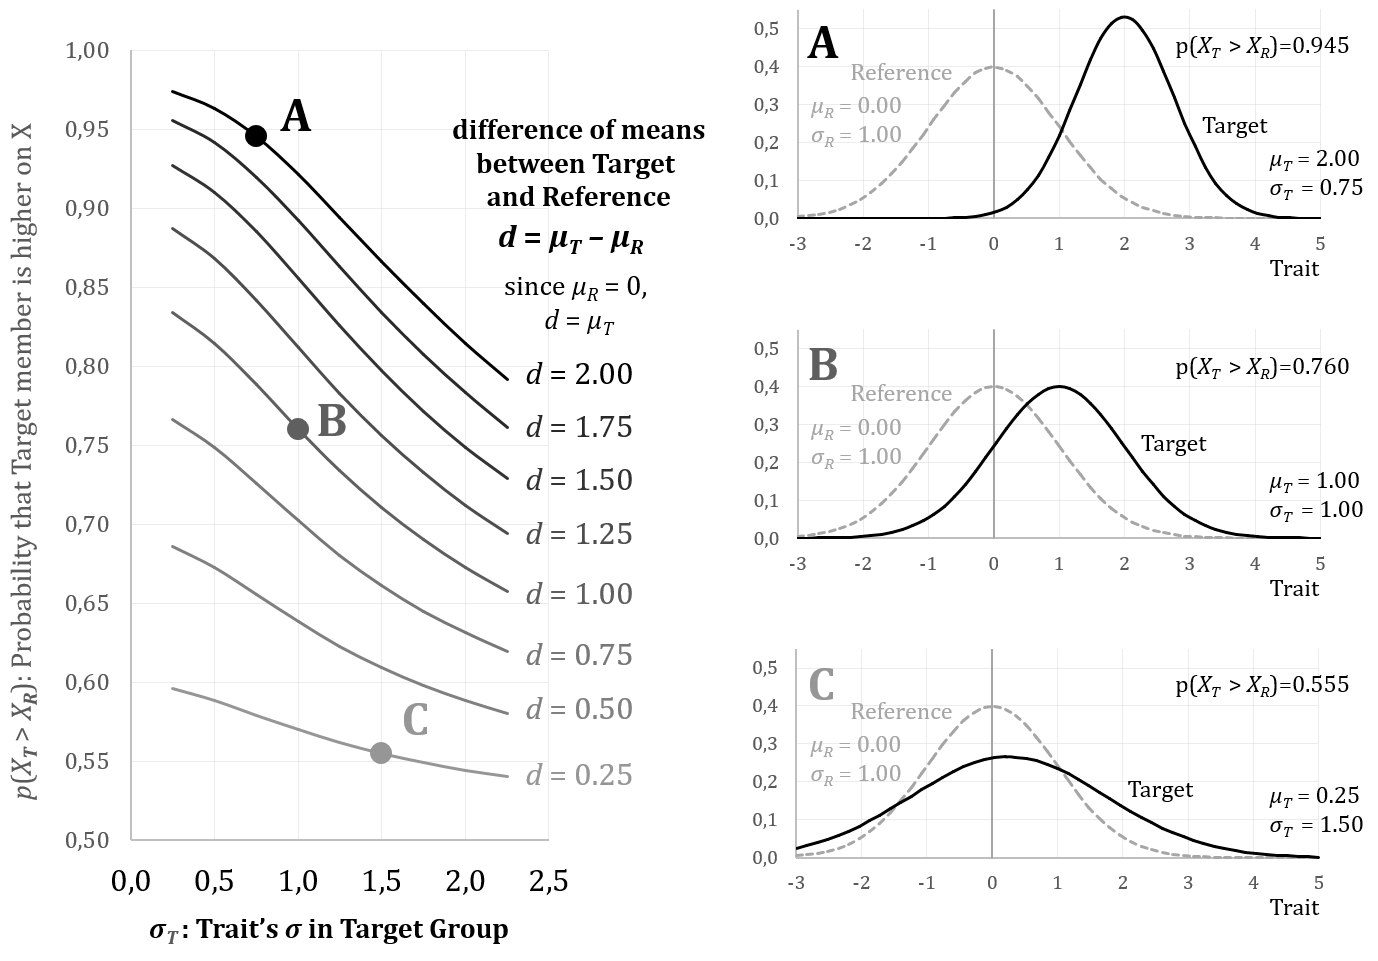
\includegraphics[width=\textwidth]{ART_Czarnik/Czarnik-img009.jpg}
\caption{Probability of a stereotype being true depending on the overlap of the trait's distributions in the target and reference group.}\label{fig1-czar}
\end{figure}



To make the link between the probability that \(X_{T} > X_{R}\) and the
relative location of the two distributions more intuitive, three
situations have been singled out for inspection:

\begin{enumerate}
\item
  \(\mu_{T} = 2.00\) and \(\sigma_{T} = 0.75\), with the corresponding
  \(p\left( X_{T} > X_{R} \right) = 0.945\);
\item
  \(\mu_{T} = 1.00\) and \(\sigma_{T} = 1.00\), with the corresponding
  \(p\left( X_{T} > X_{R} \right) = 0.760\);
\item
  \(\mu_{T} = 0.25\) and \(\sigma_{T} = 1.50\), with the corresponding
  \(p\left( X_{T} > X_{R} \right) = 0.555\).
\end{enumerate}
In A, the stereotype could be considered to be very accurate as it would produce mistakes when judging individuals only 5.5\% of the time. In C, it is barely acceptable, with failure rate at 44.5\%. What about B? With the error rate at 24\% it seems quite unreliable. But before discarding it as a far-fetched overgeneralization, one should recognize that according to a popular metric proposed by
%\label{ref:RNDI9cG7tk2qD}(Cohen, 1988),
\parencite[][]{cohen_statistical_1988}, %
 this stereotype signifies a definitely large effect size. With Cohen's \textit{d} equal to 1, it is the kind of effect that any social scientist would be more than happy to find in his or her study. Moreover, let us bear in mind that for ``new areas of research inquiry,'' effect sizes of 0.2 would not be utterly uninteresting 
%\label{ref:RNDDeitIcl8zR}(Cohen, 1988, p.25).
\parencite[][p.25]{cohen_statistical_1988}. %
 And it is just the effect size of a stereotypic difference depicted by C. Why should we then subject stereotypes to higher standards of truth than scientific findings?

For continuous variables, \(p\left( X_{T} > X_{R} \right)\) may be taken
directly as an unambiguous measure of the stereotype's accuracy because
probability that both individuals will happen to have equal values on X
equals zero. Thus if we fail to observe \(X_{T} > X_{R}\), the reverse,
\(X_{T} < X_{R}\), will be true. This is emphatically not the case with
discrete variables. The smaller the number of categories on the trait
variable, the more likely it is that the two individuals will be
indistinguishable with regard to X. The number of \(X_{T} = X_{R}\)
pairs will grow at the expense of both \(X_{T} > X_{R}\) and
\(X_{T} < X_{R}\).

Figure \ref{fig2-czar} illustrates the effect of categorization on the probabilities. Three simulations were done, each involving 100 ``persons'' (50 from the target group, and 50 from the reference group). Each group of 50 values constituted a representative selection from the underlying continuous distribution with standard deviation equal to 1. In terms of Cohen's \textit{d}, simulation no. 1 exemplified a moderate size effect ( $\mu _T-\mu _R=0.5$), simulation no. 2 a large effect ( $\mu _T-\mu _R=1.0$), and simulation no. 3 a very large one ( $\mu _T-\mu _R=1.5$). In each case, 100 values from both groups were jointly ranked and grouped into 20 categories, then into 19, then 18, and so on until the final rough division into two categories: those above and those below the median. With the original continuous variables, the probabilities $p\left(X_T>X_R\right)$ were 0.64, 0.77, and 0.87 for moderate, strong, and very strong effect sizes, respectively (see the black bullet markers in Figure \ref{fig2-czar}). These probabilities decrease systematically, even though very slightly at first, with the ongoing reduction in the number of categories. Serious distortions occur when the distributions are reduced to three or, especially, two categories.\footnote{For example, $p\left(X_T>X_R\right)=0.87$ associated with a very large effect on a continuous trait, dwindles to 0.61 after reducing the trait to a dichotomy—still noticeable but far from impressive.} $X_T=X_R$ probabilities are steadily on the rise, and for the moderate effect ( $\mu _T-\mu _R=0.5$), we observe that splitting the continuum into two parts even makes $X_T=X_R$ the most likely outcome. On the positive side, probabilities are not that heavily affected by reduction to five categories—the number of points on a Likert-type scale routinely applied to measure attitudes in surveys.


\setlength{\tabcolsep}{2pt}
\begin{figure}[H]
	\begin{small}
   \begin{supertabular}{m{.32\textwidth}m{.32\textwidth}m{.32\textwidth}}
   \begin{center}
   \textbf{moderate effect size}
   \end{center} &
   \begin{center}
   \textbf{large effect size}
   \end{center} &
   \begin{center}
   \textbf{very large effect size}
   \end{center} \\
	\vskip-.3in$$\mu_{T} - \mu_{R} = 0.5$$\vskip-.3in &
    \vskip-.3in$$\mu_{T} - \mu_{R} = 1.0$$\vskip-.3in &
    \vskip-.3in$$\mu_{T} - \mu_{R} = 1.5$$\vskip-.3in \\
   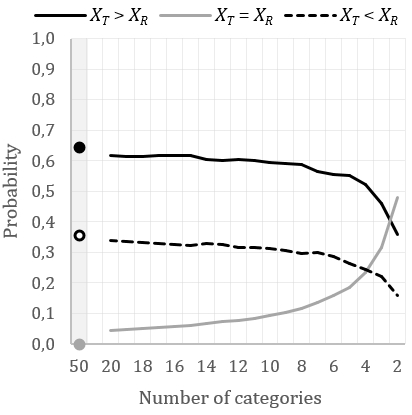
\includegraphics[width=\linewidth]{ART_Czarnik/Czarnik-img016.jpg} &
   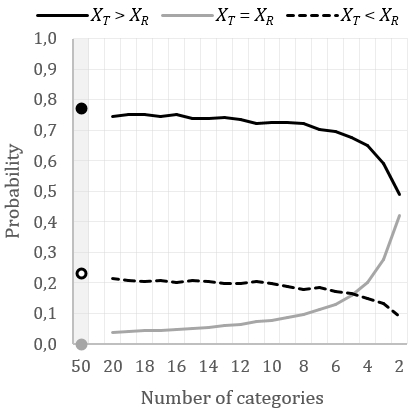
\includegraphics[width=\linewidth]{ART_Czarnik/Czarnik-img017.jpg} &
   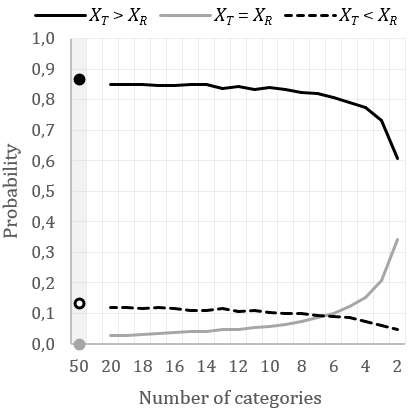
\includegraphics[width=\linewidth]{ART_Czarnik/Czarnik-img018.jpg} \\
   \end{supertabular}
   \end{small}
\caption{The effect of categorization on the observed
probabilities of \(X_{T} > X_{R}\), \(X_{T} = X_{R}\), and
\(X_{T} < X_{R}\) for three different effect sizes (all underlying
distributions are normal with \(\sigma_{T} = \sigma_{R} = 1\)).}\label{fig2-czar}
\end{figure}
When analyzing the accuracy of stereotypes regarding traits measured on
scales with a limited number of categories it is thus advisable to
consider all three possible options: \(X_{T} > X_{R}\),
\(X_{T} = X_{R}\), and \(X_{T} < X_{R}\), as it may well turn out that
\(p\left( X_{T} = X_{R} \right)\) is far from negligible.

\section{A few empirical examples of assessing the accuracy of sex stereotypes}
\enlargethispage{-2\baselineskip}
Both actual differences between the sexes and associated beliefs about these differences were intensively studied
%\label{ref:RND1zeV4PeuSF}(Williams and Best, 1982, 1990; Costa, Terracciano and McCrae, 2001; Biernat and Deaux, 2000; Buss, 2003; Pinker, 2003).
\parencites[][]{williams_measuring_1982}[][]{williams_sex_1990}[][]{costa_gender_2001}[][]{borgatta_sex_2000}[][]{buss_evolution_2003}[][]{pinker_blank_2003}. %
 In the following, I~will examine a number of possible sex stereotypes, testing their accuracy against the survey data from Polish General Social Survey 
%\label{ref:RNDDqAxDLuyEC}(Cichomski, Jerzyński and Zieliński., 2013)
\parencite[][]{cichomski_polskie_2013} %
 and the Study of Human Capital in Poland 
%\label{ref:RNDLH293GzyiT}(Górniak et al., 2015, 2019).
\parencites[][]{gorniak_bilans_2015}[][]{gorniak_bilans_2019}.%
\footnote{Representative surveys provide us with proper criteria for assessing stereotypes' accuracy. } It is irrelevant here whether most people (or any people, for that matter) subscribe to these particular stereotypes, although certainly some of the inspected traits are popularly held to be gender-differentiating (e.g. body height, earnings, interest in fashion or technology).

For each trait, probabilities of a randomly selected woman being at a
higher, the same, or lower level on the trait as compared to a randomly
selected man were computed, using the following formulae, where \emph{v}
stands for a value of the trait variable\footnote{It may be noted that a
  difference between the ``mirror-image'' probabilities, i.e.
  \(p\left( X_{F} > X_{M} \right) - p\left( X_{F} < X_{M} \right)\)\emph{,
  is equal in value to asymmetric Somer's d rank correlation coefficient
  (Somers, 1962), when predictions are based on subjects' sex.}}:
\[p\left( X_{F} > X_{M} \right) = \sum_{v = min}^{\max}{p\left( X_{F} = v \right) \bullet p\left( X_{M} < v \right)}\]

\[p\left( X_{F} = X_{M} \right) = \sum_{v = min}^{\max}{p\left( X_{F} = v \right) \bullet p\left( X_{M} = v \right)}\]

\[p\left( X_{F} < X_{M} \right) = \sum_{v = min}^{\max}{p\left( X_{F} = v \right) \bullet p\left( X_{M} > v \right)}\]

Figures \ref{fig3-czar} to \ref{fig6-czar} summarize the results.

\begin{figure}[H]
	\centering
   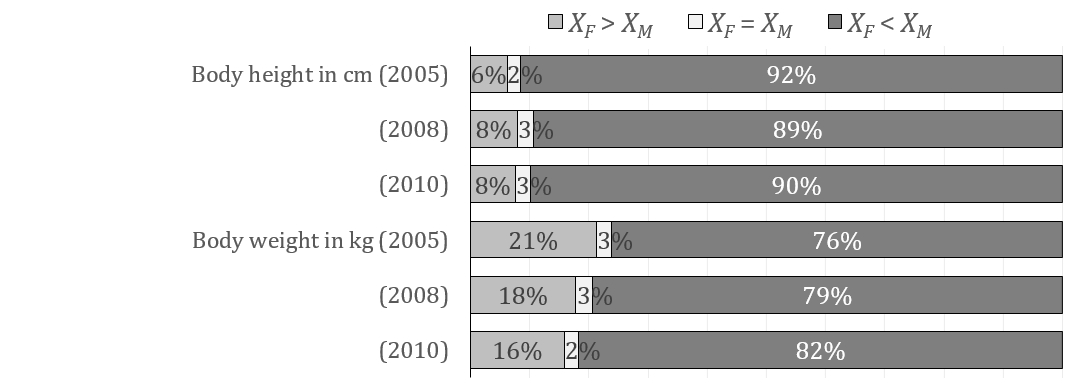
\includegraphics[width=\textwidth]{ART_Czarnik/Czarnik-img019.jpg}
\caption{Probabilistic assessment of stereotypical sex differences concerning body structure Polish General Social Survey. Open-ended questions (``What is your height and weight, approximately?'').}\label{fig3-czar}
\end{figure}


Both height and weight are near-continuous variables and therefore it's very unlikely that the two randomly selected individuals will be of the same height or weight. The probabilistic differential is very large indeed, especially with regard to height. Thus the ``men are taller than women'' stereotype will hold true for about 90\% of the randomly matched male-female pairs. It is about 12 times more likely that a man will be the taller of the two than the other way round.

\begin{figure}[H]
	\centering
   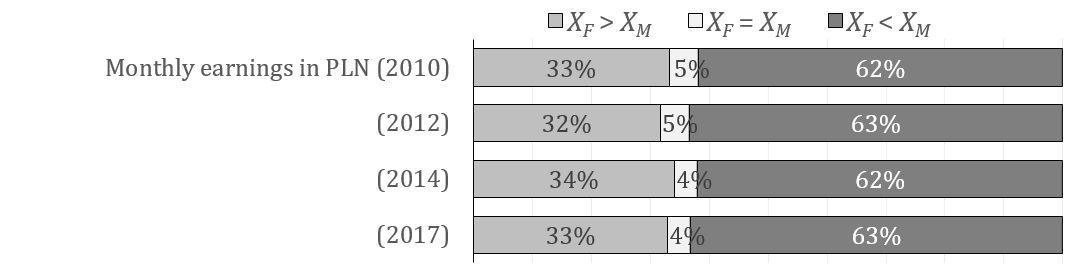
\includegraphics[width=\textwidth]{ART_Czarnik/Czarnik-img020.jpg}
\caption{Probabilistic assessment of stereotypical sex differences concerning pay* Study of Human Capital in Poland. Open-ended question with supplementary categorization. \\ * Data for employees with job contracts working full-time within last month, excluding the self-employed.}\label{fig4-czar}
\end{figure}

Sex difference in average remuneration, widely publicized under the heading of ``gender pay gap'', is common knowledge these days. However, the stereotypic assertion that men earn more than women is a rule with quite a lot of exceptions. In Poland, it is correct for more than 60\% of the random individual comparisons, yet every third time the reverse is true. Interestingly, hardly anybody is prompted by such substantial amount of ``counterevidence'' to dismiss male-female wage differential as a mere stereotype.\footnote{Similarly, Browne
%\label{ref:RNDKyToDmIZds}(1998)
\parencite*[][]{browne_divided_1998} %
 observes that while temperamental differences between the sexes (e.g. in competitiveness and risk-taking) are likely to be brushed aside because they ``do not hold true for all individuals'', the very same argument is hardly ever used to shrug off the economic differences. } On the contrary, the issue is widely researched, prominent in political agendas, and dealt with in antidiscrimination legislation.

\begin{figure}[H]
	\centering
   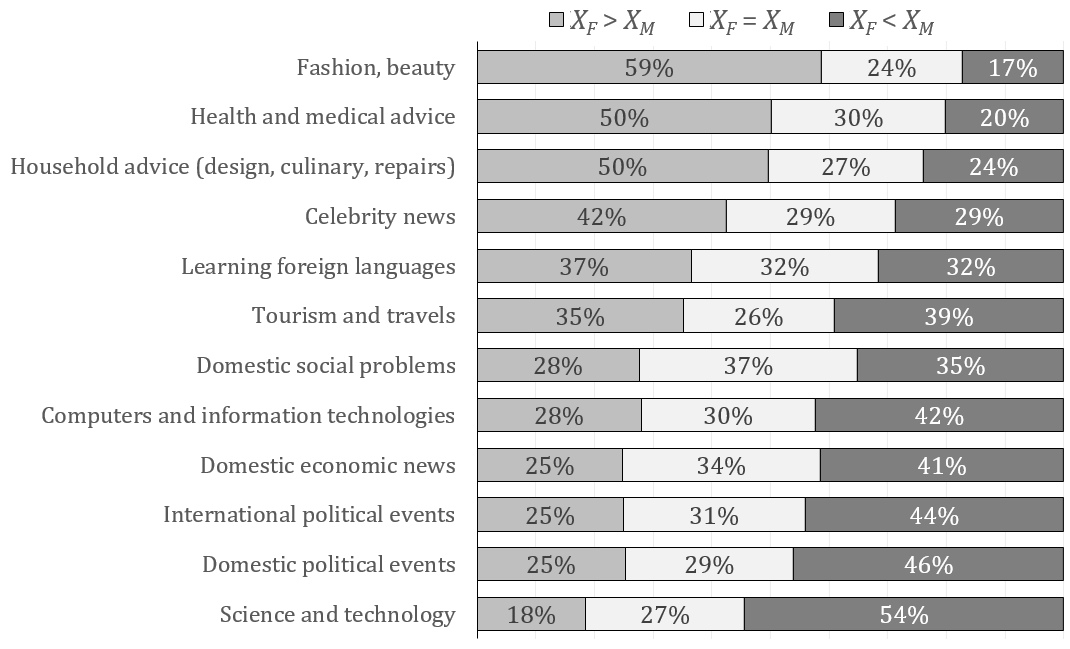
\includegraphics[width=\textwidth]{ART_Czarnik/Czarnik-img021.jpg}
\caption{Probabilistic assessment of stereotypical sex differences concerning interest in the mass media content Polish General Social Survey (2002). Interest measured on a 4-point scale: 1 not at all /2 not much /3 quite a bit /4 very much.}\label{fig5-czar}
\end{figure}

In Figure \ref{fig5-czar}, people's interests are sorted by gender differences, from those most typical of women at the top to those most typical of men, at the bottom. Some of those differences are congruent with popular sex stereotypes (e.g. those concerning fashion or technology), but even then many exceptions arise. As may be expected for traits measured using categorical scales, a substantial number of male-female comparisons produce gender-equal outcomes. Still, it is unsurprising why someone seeking medical advice from a random stranger would turn for help to a woman rather than a man. As far as a man and a woman differ in their levels of medical interests and as far as the intensity of such expressed interests is proportional to actual cognizance, it is a woman who is about 2.5 times more likely to have some acquaintance with health topics. By the same token, if one seeks technological advice, it's three times more likely that of any two random strangers, one man and one woman, the man will be the one more up-to-date with matters of technology.

\begin{figure}[h]
	\centering
   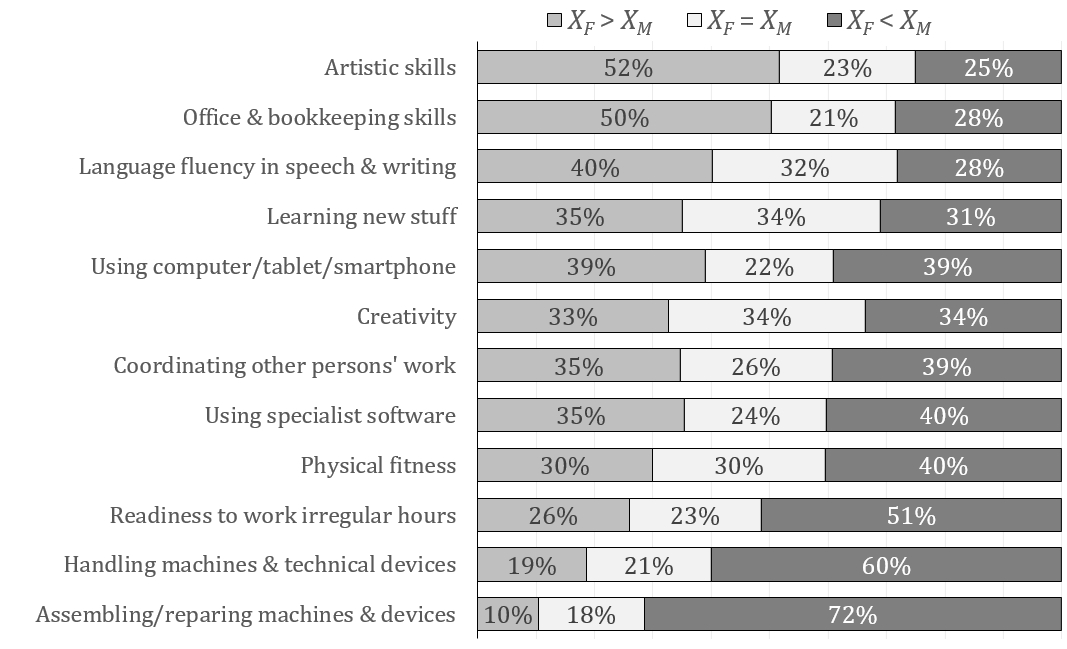
\includegraphics[width=\textwidth]{ART_Czarnik/Czarnik-img022.jpg}
\caption{Probabilistic assessment of stereotypical sex differences concerning skill self-evaluation Study of Human Capital in Poland (2017). Skill level self-valuated on a 5-point scale: 1 low /2 basic /3 medium /4 high /5 very high.}\label{fig6-czar}
\end{figure}

One can observe that stereotypical disparities in skill self-evaluations are in accord with the kinds of jobs men and women tend to perform in the gender-segregated labor market
%\label{ref:RNDeyzjhDc1o6}(Czarnik and Kasparek, 2015).
\parencite[][]{czarnik_gender_2015}. %
 The probabilistic skill differentials are most pronounced in the areas heavily dominated by either sex, i.e. clerical jobs associated with office and bookkeeping skills (women) and jobs in industry, construction, and transportation involving machines and technological environment (men). On the other hand, we see that ``men perceive themselves to be natural managers'' kind of stereotype is true by such a thin margin that it's hardly worth mentioning (see ``Coordinating other persons' work'').

\section{How good are people in assessing accuracy of stereotypes?}
As shown above, stereotypic assertions in their generic formulation may vary substantially in how much truth they contain when applied at individual level and it would be very foolish of stereotype holders, namely all of us, not to recognize the fact. Fortunately, as Schneider
%\label{ref:RNDFOmE4JC32O}(2005, p.199)
\parencite*[][p.199]{schneider_psychology_2005} %
 put it, ``[n]ot always, to be sure, but still most of us are aware that stereotypes are only probabilistically true and do not apply to everyone.'' And even if it was true, as Pinker 
%\label{ref:RND9JKr0iPkC4}(2007, p.86)
\parencite*[][p.86]{pinker_stuff_2007} %
 claims, that ``[t]he image of one orb floating above another seems to come more naturally to the mind than an image of two overlapping bell curves'', people are capable of implicitly processing this kind of information to arrive at probabilistic statements. They may commit a number of mistakes in the process, as observed by Whitley and Kite 
%\label{ref:RND7JZzDeXpJE}(2010, p.100):
\parencite*[][p.100]{whitley_psychology_2010}:%


\myquote{
Research participants might be fairly accurate, for example, in their estimates of what percentage of Asians are mathematical, but they might be inaccurate in their estimate of the variability of this characteristic. If perceivers are accurate on one measure, but not the other, does their belief have a kernel of truth? This question is difficult to answer.
}

Yet this question \textit{can} be answered by applying the probabilistic approach. It is even more to the point for the very reason that it is our probabilistic beliefs that inform our decisions concerning individuals. A typical question you would ask yourself when pressed to choose, with certain aim in mind, one from two or more persons would not be ``what is the difference of means between the groups to which these persons belong?'', and even less ``how large is the dispersion of the relevant characteristic?''. It would be ``which one of them is most likely to give me what I need?''. This probabilistic perception can easily be measured by asking people to imagine a familiar situation and make the assessment of comparative probabilities. By means of an illustration, consider how subjects could assess the accuracy of the stereotypic ``men are taller than women'' assertion.

\myquote{
Imagine that you enter an elevator in a large shopping mall and two random persons—one man and one woman—unknown to you and to each other,\footnote{It is important to exclude the possibility that a man and a woman are a couple, so that subjects' judgment about general differences would not be contaminated by their beliefs about relative height of mated individuals. } enter after you. How likely it is that: (1) the man will be the taller of the two, (2) the woman will be the taller of the two, (3) they will be of equal height (with precision of, say, 1 cm). Make sure that probabilities add to 100\%.\footnote{It is a subject for some experimentation to find out how this task could be facilitated by a particular method of registering the probabilities (e.g. by a visual representation of probabilities on screen). }
}

A very welcome aspect of this approach is that it explicitly tackles the question of whether subjects' beliefs about certain group(s) of people are of a rigid, all-or-none, kind. This should provide solid empirical evidence to inform the dispute over sensibility of making stereotypes untrue by definition. In all likelihood, for many traits it will turn out that actually very few people incorrectly perceive the stereotyped group(s) as completely homogeneous.

Subjective probabilities elicited in this way could then be compared to the factual probabilities calculated from the source data, e.g. representative survey. For example, in the particular case of the male-female height comparison, my educated guess—informed by a number of informal trials—would be that people tend to \textit{under}estimate the accuracy of the height stereotype.

To be sure, we still should be cautious not to make too much of such evidence. It is entirely plausible that even if people make nuanced probabilistic judgments when explicitly prompted to make them, they can still—especially in the absence of such prompts—behave automatically and unreflectively fall prey to the rigid all-or-nothing kind of thinking when making their everyday decisions. I think that an especially worthwhile avenue for further research is to investigate the relationship between the perceived accuracy of a given stereotype and perceiver's openness to, or even active seeking of, individuating information when making decisions.

\section{Conclusion}
Since the introduction of the concept into academic realm, a topic of stereotype accuracy was and remains controversial. As negative stereotypes have been linked to prejudice and discrimination, it seemed justified to view stereotypic beliefs as anything but accurate depictions of reality. However, this wholesale dismissal, insofar as it extends to all perceptions of group differences, has serious disadvantages. First, the larger the actual differences between the groups, the more obvious it is that the stereotype is (to some extent) accurate, and all statements to the contrary sound deceitful. In effect, all efforts at eradicating demonstrably false stereotypes may be hindered, as the criticism of stereotypes will lose its \textit{prima facie} credibility. Second, outright denial of group differences where they do exist and contribute to the perceived inequality between groups severely restricts the repertoire of actions that could be taken to address the problem.

Even if many group differences turn out to be real rather than imaginary, bigots—to reiterate Kenny
%\label{ref:RND84Zh1FAM8u}(Kenny, 1994, p.212)
\parencite*[][p.212]{kenny_interpersonal_1994}%
—``should not take any comfort in these conclusions.''\footnote{Bigots should also be well advised to recognize that they themselves are a strongly stereotyped group, and these stereotypes may turn out to be not so far from the truth, either. } Such differences leave space—in some instances a whole lot of space—for exceptions. They also evolve: they may grow bigger, but equally likely they may grow smaller, vanish or even be reversed. In any case, to minimize the stereotype-based discrimination, it is always advisable to advocate the individualistic approach, i.e. to explain why the best decisions are the ones based—whenever possible and to whatever extent feasible—on person's individual characteristics rather than on the average characteristics of the groups individuals belong to.

Testing stereotype's accuracy in probabilistic terms has a direct advantage of bridging the gap between collective and individual levels of analysis, both of which are explicitly involved in making probabilistic comparisons. This, to satisfy Jussim
%\label{ref:RNDerlUautrYn}(2012, p.309),
\parencite*[][p.309]{jussim_social_2012}, %
 should bring ``greater conceptual clarity […] to understanding stereotype accuracy.'' It could also be a step towards meeting concerns voiced by Stangor 
%\label{ref:RNDs3zgPwUmNI}(1995, p.278)
\parencite*[][p.278]{lee_content_1995} %
 that in order to find ``an adequate remedy for negative intergroup behavior […] We need to know both how big existing group differences are and how to communicate the extent of those differences to people.'' It seems that probabilistic approach is quite a promising avenue in this regard by explicitly bringing up counterexamples to the stereotype under question.

In the end, no matter how much—or how little—truth any particular stereotypes may contain, ``what matters is […] the gullibility with which we employ them''. And we would be wise indeed to take this advice from Walter Lippmann, which is no less prudent today than it was a hundred years ago:

\myquote{
if our philosophy tells us that each man is only a small part of the world, that his intelligence catches at best only phases and aspects in a coarse net of ideas, then, when we use our stereotypes, we tend to know that they are only stereotypes, to hold them lightly, to modify them gladly
%\label{ref:RNDTWIiYL2CPo}(Lippmann, 1998, pp.90–91).
\parencite[][pp.90–91]{lippmann_public_1998}.%
}


\paragraph{Acknowledgment}
Insightful comments by two anonymous reviewers and a mathematical consultation from Dr. Paweł Hołobut (IPPT PAN) are gratefully acknowledged.

\end{artengenv}


\begin{artengenv}{Sebastian J. Szybka}
	{Some remarks on the first image of a black hole}
	{Some remarks on the first image of a black hole}
	{Some remarks on the first image of a black hole}
	{Astronomical Observatory, Jagiellonian University\\
	Copernicus Center for Interdisciplinary Studies}
	{On the 10\textsuperscript{th} of April, 2019 the Event Horizon Telescope Collaboration presented the first image of the black hole. The image was obtained with a planet-scale array of eight ground-based radio telescopes. The observation relied on a technique called very long base interferometry which synchronises telescope facilities around the world. The image of a black hole together with the recent detections of gravitational waves confirms one of the most intriguing predictions of Einstein's gravity theory, namely, the existence of black holes. I will provide more details on this remarkable observation and explore its consequences for our understanding of nature. The physical reality of black holes is strongly supported by recent advances of astronomy. I claim that this fact is the key to understanding the relation between our world and the world of mathematics.}
	{black holes, event horizon, general relativity, interferometry, astronomy, Einstein, geometry.}


\section{Introduction}
\indent \lettrine[loversize=0.13,lines=2,lraise=-0.05,nindent=0em,findent=0.2pt]%
{T}{}he mysterious relation between mathematics and physical world was and still is a subject of a debate \parencite{wigner_unreasonable_1960}. From the standpoint of a theoretical physicist, but not a professional philosopher, I must admit that existence of black holes is one of the sharpest proofs of the idea that underlying structure of the physical world is of the mathematical nature. 

Black holes are the essence of general relativity. After one learns general relativity and the mathematics of black holes, one cannot help feeling that one has gained some deep insight into how nature works\footnote{Paraphrasing the words of Robert Wald \parencite*{wald_general_1984}.}.  However, as pointed out by Richard Feynman \parencite*{feynman_character_1967}, this feeling is based on a personal experience and as such is not easy to communicate outside physicist's scientific community because  [without mathematics---author's note] \textit{it is difficult to get across a real feeling as to the beauty, the deepest beauty, of nature}. Although \textit{physicists cannot make a conversion to any other language} [than mathematics---author's note], I believe, that from time to time, all of us are given a chance to appreciate a glimpse of the nature's beauty directly with our senses, just by looking at it. Recently, a glimpse of a charm of black holes was revealed to millions of people around the globe.

The scientific impact of the first image of a black hole may be less profound than the impact of the recent gravitational waves detections, but seeing is believing. The image of the black hole presented to the public by the Event Horizon Telescope Collaboration\footnote{The results were published on the 10\textsuperscript{th} of April in the six papers in a special issue of \textit{The Astrophysical Journal Letters}, \parencite[see e.g.][]{the_event_horizon_telescope_collaboration_first_2019}. More about Event Horizon Telescope Collaboration, \parencite[see][]{noauthor_event_nodate}.} is groundbreaking for the perception of black holes as real objects, especially beyond the scientific community. 

\section{Black holes}

Black holes are fascinating objects because there are made only from our concepts of space and time\footnote{The most important black hole spacetimes are given by the solutions to the vacuum Einstein's equations.}---no matter involved! They are regions of `no return' separated from the remaining part of the Universe by the boundary called an event horizon. Their existence is essential for our understanding of what time and space are. 

The history of black holes is integral to understanding the relation between real world and mathematics \parencite{malec_black_2018}. If we skip Newtonian `dark stars' and move directly to proper Einsteinian black holes, than a remarkable fact must be mentioned. The black hole concept was not invented by anyone. As far as I know, existence of objects made of space and time not only exceed imagination of scientists, but even seemingly unfettered imagination of storytellers. The existence of black holes was dictated to us by the mathematical structure of Einstein's general relativity. In fact, many scientists, including the father of general relativity---Albert Einstein---were very reluctant to accept their physical reality.

Not only origins of black holes were mathematical. As we believe today, the real astrophysical black holes are macroscopic physical objects which have properties that are believed to be typical for mathematical structures (not physical one). The mathematical model of a coffee cup is only an approximation---it is \textit{similar} to the physical coffee cup. The model may be, of course, useful in, e.g., calculating the volume of the coffee cup. Two coffee cups, even if they belong to the same tableware, are never identical, so a single mathematical model cannot be identified with them. Definitely, the mathematical model of the coffee cup is not a coffee cup. In contrast to that, electrons and their mathematical description cannot be easily separated. For example, we have a good reason to believe that the electric charge of one of the electrons in my body and the electric charge of one of the electrons in the distant galaxy billions light years away are exactly the same. Electrons' charges are identical. Two electrons are not like two cups from the same tableware. If we neglect their extrinsic properties, they cannot be distinguished at all.  The property of being \textit{identical}, in contrast to being \textit{similar}, is a mathematical property not a physical one \parencite{staruszkiewicz_filozofia_2001}. Of course, our contemporary mathematical description of the electron is not `an electron.' However, it seems that the mathematical structure which we have discovered seems to approximate the deeper mathematical structures which cannot be separated from the physical objects they define. In electrodynamics, the equality of electric charges of electrons does not follow from any basic principles, but was introduced by physicists to obtain the theory that matches observations. Nevertheless, this property of electrons fits to the physical world so well that is seems indispensable in any future theory of electrons.\footnote{Such strange coincidences are known in the history of physics. In the Newtonian mechanics, gravitational mass and inertial mass of a body are separate concepts. The equality of both masses was an assumption which needed to be confirmed by observations. In contrast to that in the Einstein's theory, gravitational mass and inertial mass correspond to a single concept---they are `the same.'}

For us, the microscopic world of particles is elusive because it is not directly accessible to our senses.  The black holes are macroscopic objects that share with electrons this amazing property of being realisations of a simple mathematical structure. The charges of two electrons are indistinguishable in the same sense as two equal numbers are identical. Whenever a stationary astrophysical black hole has a several solar masses or billions of solar masses it is defined by only two parameters: the mass and angular momentum. This universality extends over ten orders of magnitude. Any two such black holes are identical (if we ignore different values of parameters), in the same sense, as two mathematical functions are. In contrast to electrons, astrophysical black holes are large which makes them, in principle, accessible to our senses. Observations of them reveal directly mathematical nature of reality. As pointed out by the world-famous astrophysicist and Nobel laureate Subrahmanyan Chandrasekhar \parencite*{chandrasekhar_shakespeare_1975}:

\myquote{
In my entire scientific life, extending over forty-five years, the most shattering experience has been the realization that an exact solution of Einstein's equations of general relativity, discovered by the New Zealand mathematician Roy Kerr, provides the absolute exact representation of untold numbers of massive black holes that populate the universe. This ``shuddering before the beautiful'' this incredible fact that a discovery motivated by a search after the beautiful in mathematics should find its exact replica in Nature, persuades me to say that beauty is that to which the human mind responds at its deepest and most profound level.}

There is at least one more important secret hidden inside of black holes. The edge of the Universe is usually related to the so-called particle horizon. This boundary of the observable Universe is really far away. Although we cannot observe what lays behind it, we have some reasons to believe that nothing unusual happens there. The true mysterious edge of spacetime is not there, but, in the cosmological scales, it lays just behind the corner. The Einstein's gravity theory---general relativity---predicts its own breakdown inside of the black holes. This means that space and time, as we know it, ends there. Therefore, the black holes are true gates to the unknown territory that cannot be explored without the new physics.

\section{Casting call}

If we look at a night sky with naked eyes, we see mainly photons emitted by Milky Way stars. However, if we observe a sky with a help of a radio telescope, one of the brightest sources are massive black holes (black holes are black, but the accreting matter radiates energy away). In this sense, we have already indirectly observed black holes for many years. However, by \textit{seeing} one usually means to see a shape of an object. This is not easy task for astronomers. The universe is vast, distances are huge. Modern sky surveys catalogue billions of stars, but, only images of several dozen of them has been resolved. Majority of stars are seen as point sources. 

Taking an image of a black hole is a formidable task. Masses of some galactic black holes may reach dozens of billion of solar masses, but black holes are most compact objects in the Universe. For example, the black hole with the mass equal to the mass of Earth is really tiny---its radius is only about $9$ mm. 

As we known today, astrophysical black holes exist in two sizes. The so-called stellar black holes with masses ranging from several to dozens of solar masses are created as an end state of evolution of massive stars. The so-called galactic black holes (or supermassive black holes) with masses ranging from hundreds of thousands to tens of billions of solar masses reside in the center of galaxies. The black holes are black, so good candidates for taking an image must be active---they must swallow the surrounding matter:  a cosmic dust, a gas, stars. The matter falling on a black hole radiates huge amount of energy which lighten up the neighbourhood and creates the black hole shadow. The black hole shadow contains the event horizon, thus we expected to see a gate to the region of `no return.' The candidates must also have possibly large angular size---this parameter is crucial for resolving images. It turns out that in this competition the supermassive black holes are clear winners. The Event Horizon Telescope team picked out two candidates: the nearest supermassive black hole Sgr A* at the center of our galaxy and much bigger supermassive black hole at the center of the galaxy M87. Our supermassive black gole Sgr A* is about 26000 light years away from Earth and has about four million solar masses. The M87 black hole is about 1500 times more massive and 2000 times further away. It follows from this comparison that the size of the M87 black hole event horizon is only about 22 micro-arc-sec of a degree compared to 53 micro-arc-sec of a degree of Sgr A*. Nevertheless, the M87 black hole turned out to be a better candidate. Although the Event Horizon Telescope team attempted to create images of both black holes only the image of the M87 black hole was presented on the 10\textsuperscript{th} of April 2019. The center of our galaxy is not a best direction to conduct this kind of imaging. The larger mass of the M87 black hole implies that the image change less during observation time which guarantees more stable condition for taking an image. Photographing a running athlete with long exposure time is definitely much harder than taking a photo of grandparents behind a table!

\section{Your camera matters}

How to create an image of a black hole? Since the event horizon of the M87 black hole is about 22 micro-arc-sec of a degree as seen from Earth, an extreme resolution is needed. A resolution of a human eye is about 60 arc-sec of a degree. The Hubble telescope is much better having a resolution about 0.05 arc-sec of a degree, but still nowhere close to what is needed. We need an instrument which would allow a person sitting in Kraków to read a newspaper in New York! A simple rule says: the larger diameter of the lens the higher resolution. The formula which is necessary to estimate the size of the instrument has a trivial form. The resolution of an astronomical instrument is about $\lambda/D$ where $\lambda$ is the wavelength of the electromagnetic radiation at which we want to observe and $D$ is the size of the instrument. Firstly, the Event Horizon Telescope team had to decide at which wavelength they want to observe a black hole. Several factors must be taken into account here: longer wavelengths require bigger instruments, the M87 black hole should look interesting at a given wavelength, wavelengths at which the Earth-based astronomical observations are conducted are strictly restricted by absorption of the Earth's atmosphere. Majority of people would like to have a photograph of a black hole and by that they usually mean: in the visible light. However, the wavelength of the electromagnetic waves is not their fundamental property---it depends on the observer who measures them. There is no fundamental difference between photons associated to the visible light and those associated to radio waves. The techniques used to capture them differs because these photons have different energies relative to us, but what is infrared radiation for one observer may be visible light to another observer who moves relative to the first one at relativistic speed. Therefore, for a professional astronomer the image of the black hole in different part of the electromagnetic spectrum than the visible range is not less `true' nor interesting than a photograph in the visible light. (Even cameras in ordinary mobile phones go slightly beyond visible part of the spectrum.) Moreover, it was expected that our black holes do not look attractive from this distance in the visible light---they would probably look more like an ordinary stars and we would not see a black hole shadow. Observations in standard radio waves were not convenient because necessary resolution would imply too large size of the instruments (from formula $\lambda/D$). It turned out that the wavelength $1.3$ mm is the best choice: it was expected that we will see the black hole shadow, there is the so-called `atmospheric window' at this wavelength (a tiny one), and, what a lucky coincidence, the M87 black hole is just at the right distance, hence, the instrument has the largest admissible size---the size of Earth!

Of course, building an astronomical instruments of the size of Earth is not for faint-hearted. Astronomical instruments used to detect electromagnetic waves at $1.3$ mm do not resemble optical telescopes. They are radio telescopes and have a form of a satellite antenna---a dish. The world-largest radio dish telescope FAST has a $500$ m aperture (and a fixed dish). Several years ago building a radio telescope of the size of Earth would not be possible at all. However, recently, the technique called the very long base line interferometry (VLBI) has been developed and successfully applied in astronomical observations. 

Imagine that the dish of our satellite antenna has a hole. It will still work, but less efficiently. The size of the astronomical instrument $D$ that enters the formula for a resolution $\lambda/D$ denotes the distance between most distant parts of our instrument. Therefore, a dish with many holes would have the same resolution as the dish without holes, but the signal would be much weaker. The basic idea of the VLBI technique is to use many different instruments spread across the globe and integrate the signal. Thus, all of them may work as a single instrument. The clear advantage of this method is that there is no need to build a new instrument and one may use pre-existing infrastructure. The basics of this technique has been established many years ago, but only recently the technical difficulties were overcome. The highly non-trivial task is to correlate the signal between different instruments. One should know with extremely high precision when the signal arrived. Clocks at different observatories must be precise and synchronized. A delay of the signal that is usually induced by the telescope electronics, must be estimated to high accuracy. All these goals were achieved by the Event Horizon Telescope team. The atomic clocks used to time-stamp data were hydrogen masers. These clocks lose only one second in every 100 million years. The required synchronisation obtained with the Global Positioning System was at the level of a millionth of a second.

The signal from the black hole which the Event Horizon Telescope Collaboration was going to observe was weak. In fact, it was billion times weaker than the electromagnetic signal received by an old-fashion TV antenna. Nevertheless, the array of eight radio telescopes (ALMA, APEX, the IRAM 30-meter telescope, the James Clerk Maxwell Telescope, the Large Millimeter Telescope Alfonso Serrano, the Submillimeter Array, the Submillimeter Telescope, and the South Pole Telescope) was powerful enough to observe the M87 black hole during a week long session. (The Event Horizon Telescope project has been in the works for two decades to make this observations possible.) The radio telescopes do not create images as `single shots.' They rather work like scanners which measure intensity of the radiation at a given point. The instruments recorded hundreds of petabytes of data which was combined into a single image by supercomputers at the Max Planck Institute for Radio Astronomy and MIT Haystack Observatory. (What is interesting, it was faster to transport hard disks with data on planes than send data in a digital form over internet.) 

\section{Seeing is believing}

The image of the black hole at the center of the galaxy M87 is presented in figure \ref{bh}. The black hole was observed at a single wavelength $1.3$ mm, thus the gradation in color\edtfootnote{The printed format of this article contains black-and-white graphics, the electronic format is prepared in color.} does not corresponds to different wavelengths, but to the brightness (colors are artificial). The matter falling onto black hole forms an accretion disk. It is heated and glows. The gravity bends light which forms a bright ring around a dark shadow of the black hole. For a non-spinning black hole (but this black hole is spinning) the inner radius of the ring is about $2.6$ times bigger then the radius of the event horizon. At first sight, it looks like we see the M87 black hole in the direction perpendicular to the disk. This is not true. The light rays are bend so strongly that we see also the part of the accretion disk which should be hidden behind the black hole. One part of the ring is brighter, because of the so-called relativistic beaming effect: the increased brightness implies that this part of the accretion disk rotates towards us.
%
\begin{figure}[t!]
\begin{center}
%
\includegraphics[width=\textwidth]{ART_Szybka/szybka-imgbw.png}
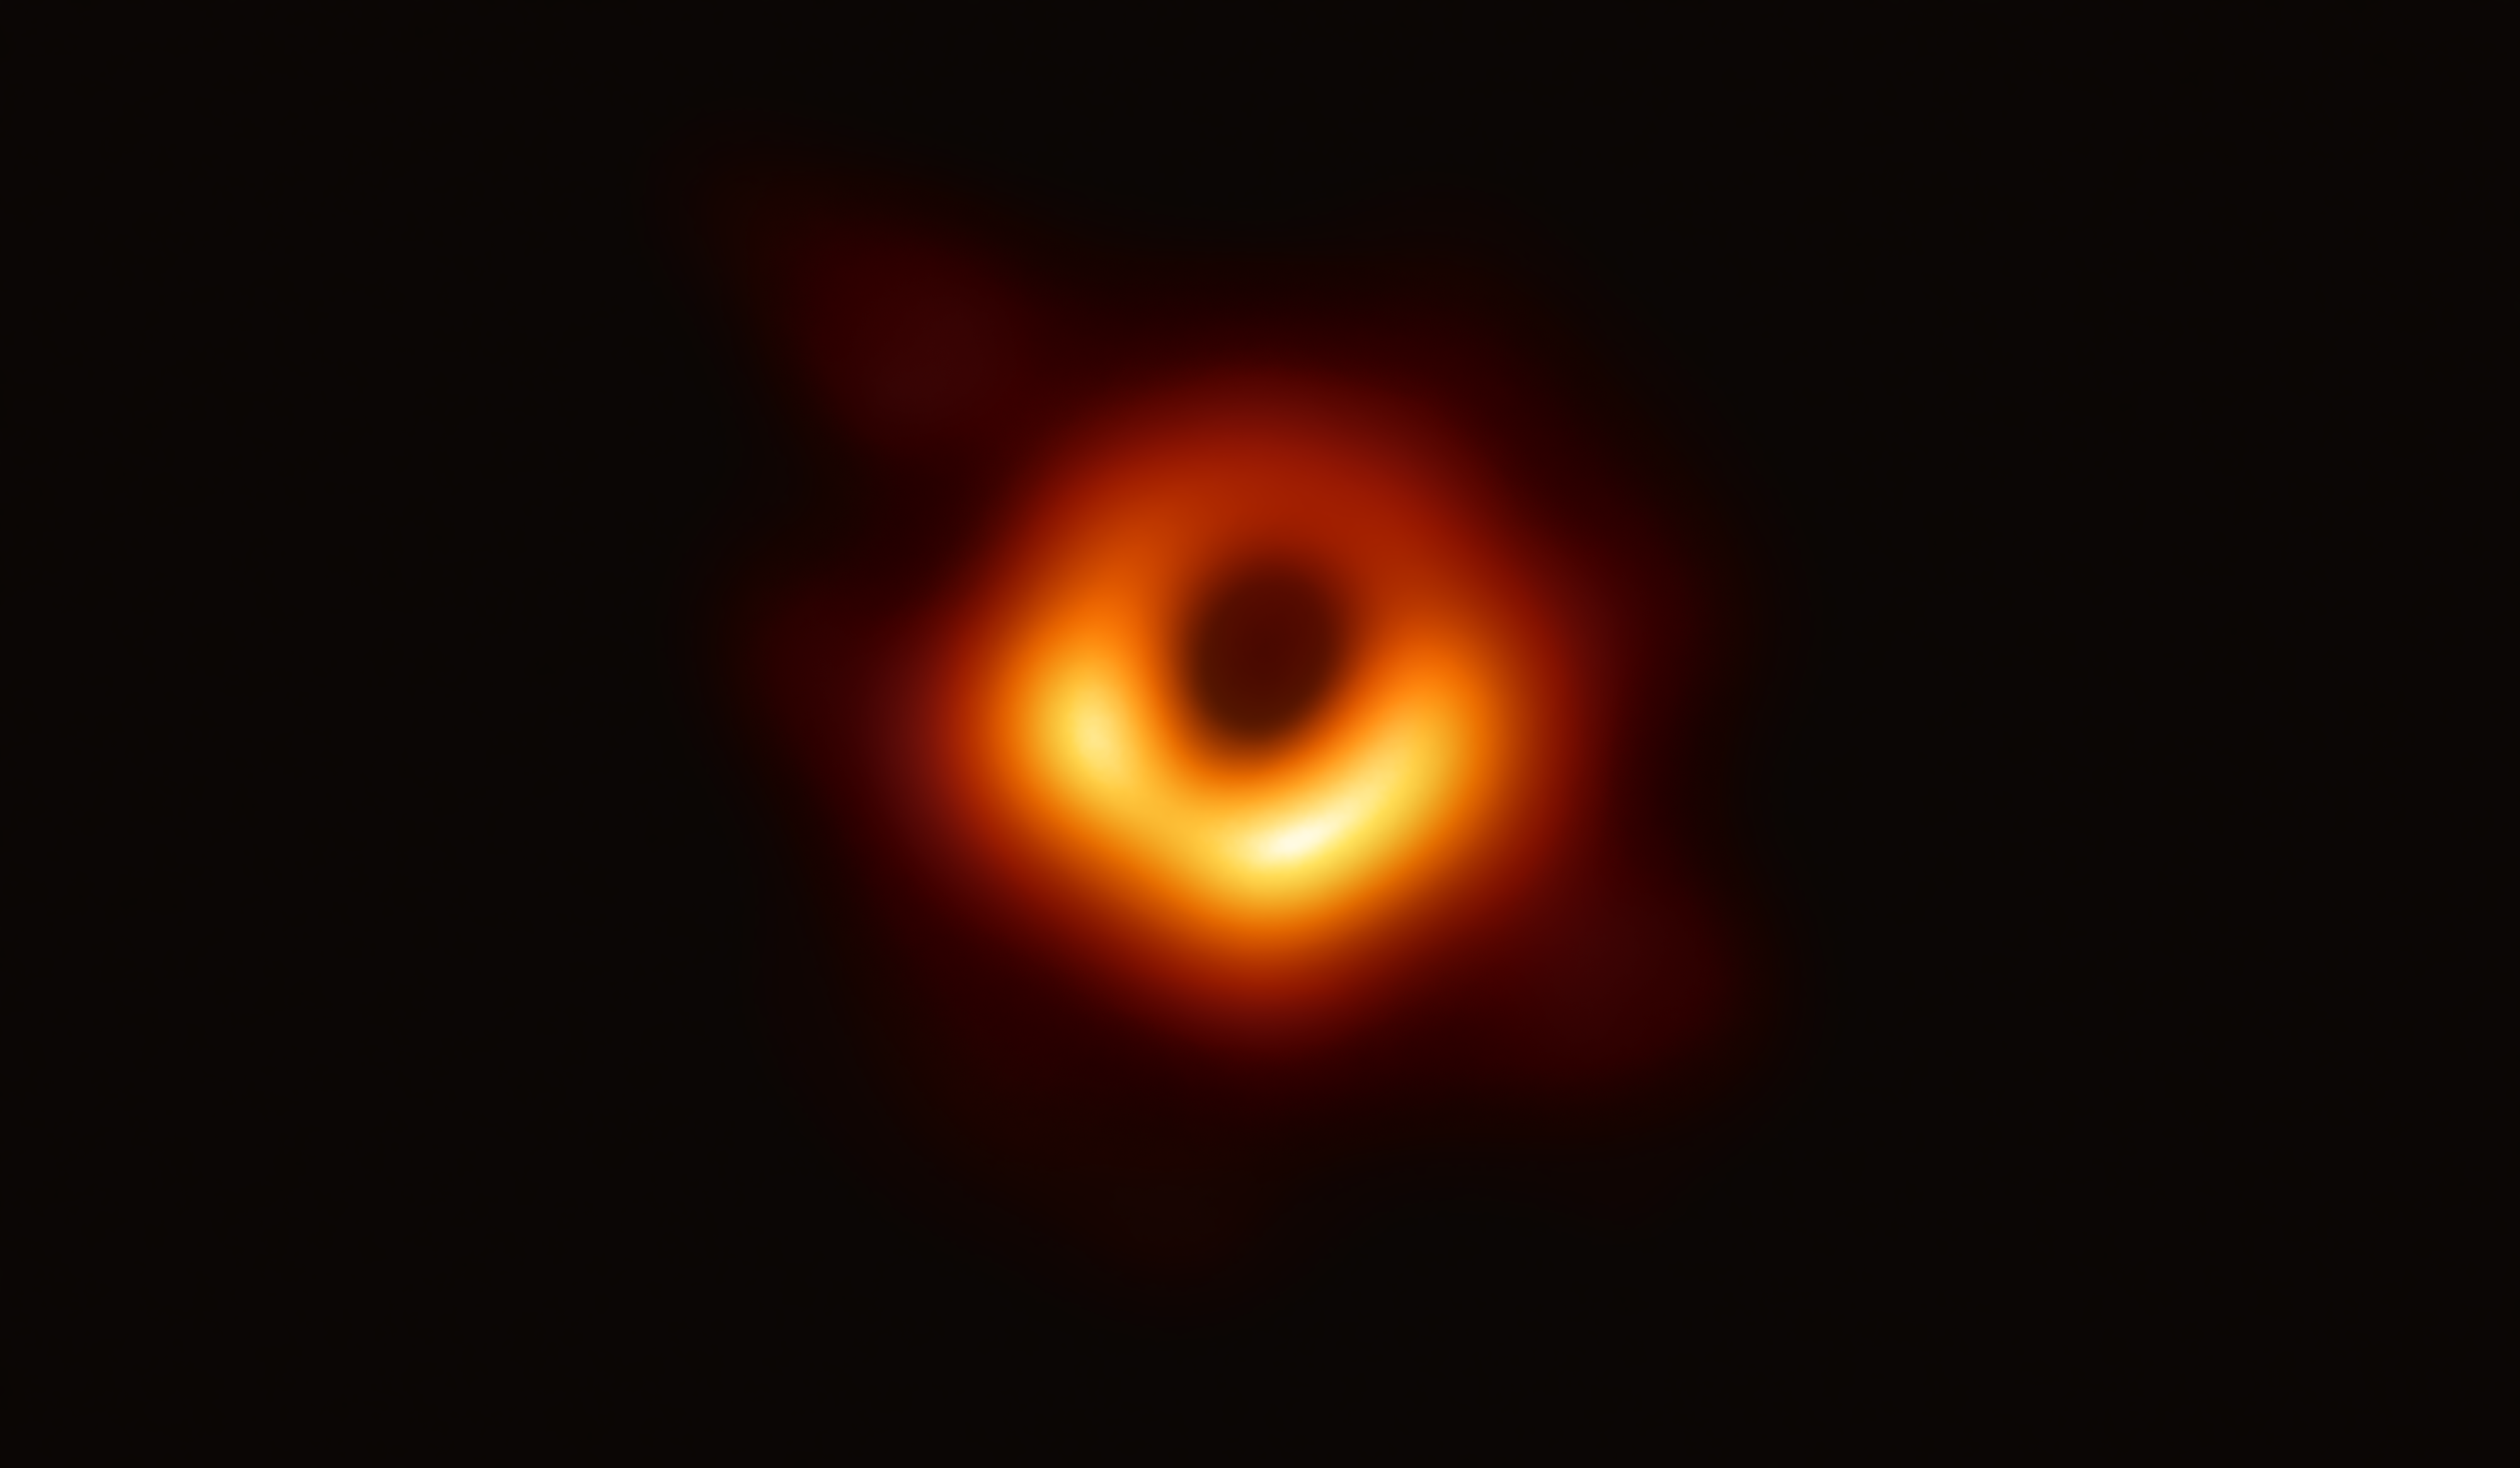
\includegraphics[width=\textwidth]{ART_Szybka/szybka-img.png}
\caption{The image of the supermassive black hole at the center of the galaxy M87 (the black hole is $6.5$ billion times more massive than the Sun). The matter falling on the black hole shines radiating energy away. The extreme gravity curves light which forms a bright ring in the image. At the center of the ring a dark silhouette of the black hole is clearly visible. This shadow contains the event horizon. Credit: Event Horizon Telescope Collaboration.}
\label{bh}
\end{center}
\end{figure}
%

 The M87 black hole is 55 million light year from Earth and is 6.5 million times more massive than the Sun. Its event horizon radius is about $120$ times larger than the distance from Earth to the Sun (three times larger than the average distance between Pluto and the Sun).

The first image of the black hole (figure \ref{bh}) is consistent with general relativity. Of course, there are many other images that would be consistent with the Einstein's gravity theory (depending on the parameters of the system), thus in this case it is better to talk about consistency than a direct proof of the theory. Nevertheless, many characteristic features of this image agree with predictions of general relativity and one may use it to improve estimates of the M87 black hole parameters (like a mass and a size). With a help of this image we may exclude some exotic alternatives to black holes. 

\section{Summary}

The image obtained by the Event Horizon Telescope Collaboration (with 200 scientist involved) was a spectacular example of application of very large base interferometry. The breakthrough in technology and new algorithms allowed the team to achieve something that not so long time ago was presumed to be impossible. What is even more important: the future is bright. The first image of the black hole which was presented on the 10\textsuperscript{th} of April 2019 was not a final product of the project, but just a first outcome. With more instruments joining the Event Horizon Telescope Collaboration and increased sensitivity we should expect more spectacular images of the M87 black hole and other black holes. Probably, in not so distant future, we may even expect  movies showing the black holes in action. 

The recent detections of gravitational waves from colliding black holes and the image of the black hole are remarkable achievemnts. Any doubts about the reality of black holes slowly dissolve. Their existence must be taken seriously. In my opinion, this fact sheds light on fundamental philosophical questions such as relation between the real world and mathematics. We may directly observe macroscopic physical entities which are inseparable from their mathematical description. 

For those, who have seen \textit{La Porte de l'Enfer} by August Rodin, the image of the M87 black hole may have a special poetic meaning. Look again at figure \ref{bh}. There is the event horizon at the central part of the black hole silhouette. Not far behind it a singularity is hidden. The space and time as described by modern physics ceases to exist there. Behind the curtain of the event horizon the known ends and unknown begins, the flow of time twirls. The laws of physics tells us: abandon all hope for the return, who enters here.

\end{artengenv} %bw-col



%\addtocontents{toc}{\protect\pagebreak}



\sekcja{Recenzje}{Book reviews}

\begin{recengenv}{Michael Dominic Taylor}
	{The hidden theological and philosophical presuppositions motivating the modern cosmological discussion: Why both sides are wrong}
	{The hidden theological and philosophical presuppositions motivating the modern cosmological discussion: Why both sides are wrong}
	{David Alcalde, \textit{Cosmology Without God?: The Problematic Theology Inherent in Modern Cosmology}, Cascade, Eugene 2019, pp.226.}





David Alcalde contributes to the clarification of thought on the origin of the universe from the unique position of an author who holds doctorates in both astrophysics and theology. Critiques of modern science and its limitations are increasingly necessary and increasingly common, but this work is indispensable because it approaches its subject matter from both sides of the argument. Alcalde addresses the insufficiencies of scientism and positivism cogently while explaining the unavoidability of metaphysical and theological presuppositions held by atheistic cosmologists, but he also succeeds in dismantling the unconsciously and improperly assumed presuppositions of cosmologists claiming to argue from a position of faith in favor of the beginning of the universe. Thus, this book reads both as a philosophical critique of modern science, and as a manual for Christian scientists who may be guilty of failing to comprehend what they claim to promote.

In a clear and coherent style, the author unravels the myth of modern science's supposed neutrality, while, at the same time, opening up the world of cosmological theory to readers from all backgrounds. Knowledge of highly technical language is not a requirement for comprehending the descriptions the author offers of the most important cosmological theories in discussion today: the Big Bang model, with its modifications of dark matter, inflation, and dark energy; the steady-state model; the Penrose-Hawking singularity theorem, which incorporates the theory of quantum tunneling; the no-boundary proposal of Hartle and Hawking; the so-called ``creation out of nothing'' model from Vilenkin, within which nothing is actually still something; the cyclic universe, promoted by Steinhardt and Turok; the multiverse hypothesis; and even the proposal that the universe was created by a designer (or designers) who are not gods but highly evolved aliens.

Theological extrinsicism, the position that holds that God is extrinsic to and outside of nature and therefore has no relevance to scientific problems, is prevalent in both camps who compose two sides of the same coin. On the one hand, openly atheistic scientists---Stephen Hawking, perhaps the most representative among them---go through a great deal of effort to avoid what would appear to be a beginning to the universe, because to them, this temporal beginning is too similar to what they perceive to be the creation event of the Judeo-Christian tradition. From the ``steady-state model'' to Hawking's ``no boundary proposal'' and the multiverse, Alcalde describes in detail, yet without heavy academic jargon, the many efforts employed by atheists to defend their theological beliefs. The problem, however, is that these scientists fail, philosophically and theologically, to understand the doctrine of \textit{creatio ex nihilo}. Thus, these scientists find themselves battling a straw man and sacrifice the scientific rigor of providing testable hypotheses in order to do so. The theological and philosophical presuppositions of atheistic cosmologists betray their scientific intentions.

However, what is perhaps the most valuable contribution of Alcalde's exposition is his critique of those cosmologists who claim to argue in favor of a Christian position. In the case of many of the most vocal advocates, Christian cosmologists also fail dismally to uphold the philosophical doctrine of \textit{creatio ex nihilo} defending rather the same theological extrinsicism that atheists reject. Principal among these thinkers are the philosophical theologian William Craig and the Jesuit Robert Spitzer.  Both defend the \textit{kalam} cosmological argument, which bears within it a mechanistic conception of the universe. Thus, the author reveals that mechanism is not only a problem for science but also one for theology.

Alcalde's systematic description of the arguments employed on both sides of this theological extrinsicism reveal the inescapable need for philosophical literacy, both to preserve the scientific pursuit and to prevent theology from slipping into the temptation of claiming empirical evidence as its own justification. The philosophical concept of \textit{nihil} is perhaps the \textit{crux} of Alcalde's argument. It serves both to express the gratuity of all of creation and, to remove any limitation from the act of creation itself. For both atheists and Christians, comprehending creation in this light is essential to a proper understanding of God, for, as Thomas Aquinas pointed out nearly eight centuries ago, ``…an error about creation is reflected in a false opinion about God'' (\textit{Summa Contra Gentiles}, II, 3.1). As the author shows, the simple yet radical assertion of the real distinction between essence and existence is the key to disentangling scientific investigation from theological extrincisim. Being cannot be taken for granted, as sheer facticity that is ``just there.'' But neither can scientific evidence be offered for the existence of God without predetermining an extrinsic conception of God that is un-Trinitarian and therefore not Christian, because creation and the temporal origin of the universe are two separate phenomena that occur on two separate levels.

Scientists, regardless of their theological beliefs, cannot ignore the author's cogent presentation of the doctrine of \textit{creatio ex nihilo}, which must bear on human reason in a recognition of the logical necessity of the metaphysical question \textit{par excellence}: why is there something rather than nothing? The alternative is a scientific position either elevated to a rank its condition ought not bear (as evidence of an omnipotent creator, who is not the Christian God but a ``god of the gaps'') or pushed into science fiction (e.g. a multiverse or alien designers) by an ``atheism of the gaps.'' In this sense, the ``warm reception'' the theory of the Big Bang has received by theologians is misguided and misleading, as it could never be equated with the event of creation. In both cases, scientific rigor is sacrificed in favor of theological extrinsicism, in its positive or negative sense, which the author whole-heartedly rejects. In the end, what Alcalde is fighting for is a true science, unassailed by theological Trojan horses, not because it feigns neutrality and indifference towards philosophy and theology, but because it recognizes its own proper place in the hierarchy of human knowledge.



\autorrec{Michael Dominic Taylor}

\end{recengenv}

\begin{recplenv}{Kamil Trombik}
	{Wokół myśli Józefa Życińskiego}
	{Wokół myśli Józefa Życińskiego}
	{\textit{Media -- kultura -- dialog. W~piątą rocznicę śmierci arcybiskupa Józefa Życińskiego}, red. R. Nęcek, W. Misztal, Wydawnictwo Naukowe Uniwersytetu Papieskiego Jana Pawła II w~Krakowie, Kraków 2017, ss.~343.}







Józef Życiński należał do grona najbardziej rozpoznawalnych polskich filozofów chrześcijańskich przełomu tysiącleci. Dość powiedzieć, że lubelski arcybiskup pozostawił po sobie setki publikacji filozoficznych, w~tym dziesiątki książek, wydawanych także w~językach obcych, m.in. ,,The Structure of the Metascientific Revolution -- An Essay on the Growth of Modern Science'', z~1988 roku, która ukazała się w~polskim tłumaczeniu po 25 latach dzięki Wydawnictwu Copernicus Center Press
%\label{ref:RNDfGKHqx5bSK}(Życiński, 2013).
\parencite[][]{zycinski_struktura_2013}.%
 W~tym ogromnym dorobku naukowym i~popularyzatorskim znaleźć można prace poświęcone zarówno problematyce filozofii przyrody, metodologii nauk, filozofii języka, teologii naturalnej, jak i~filozofii społecznej czy etyce. Świadczy to niewątpliwie o~rozległości zainteresowań tego myśliciela, ukształtowanego i~związanego od lat 70. XX wieku z~krakowskim środowiskiem interdyscyplinarnym\footnote{Należy dodać, że J. Życiński był współtwórcą krakowskiego Ośrodka Badań Interdyscyplinarnych i~periodyku ,,Zagadnienia Filozoficzne w~Nauce'',,wniósł także istotny wkład w~rozwój koncepcji ,,filozofii w~nauce'', 
%\label{ref:RND9ek2REd7gQ}(zob. np. Polak, 2019).
\parencite[zob. np.][]{polak_philosophy_2019}.%
}.

Nie powinno więc dziwić, że spuścizna J. Życińskiego stała się w~ostatnim okresie przedmiotem licznych dyskusji w~środowisku akademickim, zwłaszcza w~Krakowie\footnote{Warto w~tym kontekście odnotować również najnowsze prace poświęcone filozofii J. Życińskiego, jakie powstają w~środowisku krakowskim -- zob. m.in.
%\label{ref:RNDEdtOWWuDHP}(Liana, 2019).
\parencites[][]{liana_nauka_2019}[][]{liana_2020}.%
}. 11 lutego 2016 roku odbyła się tutaj ogólnopolska konferencja naukowa ,,Media -- kultura -- dialog'',,poświęcona właśnie pamięci zmarłego pięć lat wcześniej metropolity lubelskiego. W~organizację tego wydarzenia zaangażowało się wiele instytucji naukowych oraz organów samorządowych: Uniwersytet Jagielloński w~Krakowie, Uniwersytet Papieski Jana Pawła II w~Krakowie, Akademia Ignatianum, Naczelna Rada Adwokacka w~Warszawie oraz Okręgowa Rada Adwokacka w~Krakowie. Owocem tej konferencji jest m.in. omawiana monografia zbiorowa, zawierająca blisko 20 artykułów poświęconych szeroko rozumianej działalności społeczno-kulturowej J. Życińskiego, a~także okolicznościowe teksty wystąpień organizatorów i~hierarchów kościelnych, biorących udział w~konferencji\footnote{Zasadniczą część książki poprzedzają teksty wystąpień Wojciecha Nowaka (Rektora Uniwersytetu Jagiellońskiego), Gianfranco Ravasi (Przewodniczącego Papieskiej Rady do spraw Kultury), Celestino Migliore (ówczesnego Nuncjusza Apostolskiego w~Polsce), Stanisława Dziwisza (ówczesnego Metropolitę Krakowskiego), Wojciecha Zyzaka (Rektora Uniwersytetu Papieskiego Jana Pawła II). Monografię zamyka natomiast przemówienie Wojciecha Życińskiego do organizatorów i~uczestników konferencji, a~także tekst homilii bp. Grzegorza Rysia.}.

\enlargethispage{-.5\baselineskip}
Rozległość zainteresowań badawczych lubelskiego metropolity odzwierciedla rozpiętość tematyczna tekstów zawartych w~monografii. Mamy tutaj artykuły reprezentantów filozofii, wywodzących się z~różnych nurtów myślenia (m.in. Michał Heller, Jan Woleński, Jan Andrzej Kłoczowski, Alfred Wierzbicki), a~także teologii (m.in. Józef Kloch, Andrzej Draguła), literaturoznawstwa (Franciszek Ziejka), językoznawstwa (Jerzy Bartmiński), nauk społecznych (m.in. Michał Drożdż, Robert Nęcek, Wiesław Godzic), prawa (m.in. Andrzej Zoll) i~medycyny (Ewa Kucharska, Tomasz Trojanowski).

Choć omawianą książkę trudno uznać za wyczerpujące studium myśli Życińskiego, znalazło się tutaj miejsce na omówienie przynajmniej kilku istotnych aspektów jego akademickiej i~duszpasterskiej spuścizny. Jak pisał M. Heller, który przez wiele lat współpracował naukowo z~lubelskim arcybiskupem, ,,Józef Życiński jako człowiek miał wiele twarzy: twarz intelektualisty, działacza, duszpasterza, hierarchy, filozofa i~uczonego, pisarza, felietonisty o~ciętym języku, twarz wrażliwego człowieka'', (s.~25). Autorzy ukazują na kartach tej książki niektóre z~twarzy Życińskiego, przybliżając czytelnikowi złożony świat jego oryginalnej myśli filozoficznej, teologicznej i~społecznej.

Część artykułów wprost koncentruje się na problematyce filozoficznej, a~ich autorzy omawiają m.in. koncepcję pola racjonalności czy polemiki Życińskiego z~postmodernizmem\footnote{Zob. np. rozdziały M. Hellera ,,Jozefa Życińskiego idea pola racjonalności'',
%\label{ref:RNDPocXZSDkXd}(Heller, 2017)
\parencite[][]{heller_jozefa_2017}%
 i~M. Drożdża ,,Poszukiwanie sensu wobec postmodernizmu, relatywizmu i~ironii'', 
%\label{ref:RND0E7cy4NqCz}(Drożdż, 2017).
\parencite[][]{drozdz_poszukiwanie_2017}.%
}. Choć zagadnienia z~zakresu filozofii przyrody i~metodologii nauk -- czyli wiodącego obszaru zainteresowań Życińskiego -- rzadko stanowią centrum rozważań autorów tej książki, to w~licznych tekstach powraca wątek koncepcji interdyscyplinarności jako fundamentu filozofii krakowskiego myśliciela (np. s.~125–127). Poszukiwanie pomostów między naukami przyrodniczymi, humanistyką a~myślą chrześcijańską było jednym z~kluczowych elementów działalności Życińskiego, co autorzy tej książki podkreślają w~swoich artykułach dotyczących jego refleksji nad człowiekiem (zwłaszcza w~kontekście społecznym), kulturą, aksjologią, religią i~rolą Kościoła we współczesnym świecie.

Należy przy tym podkreślić, że teksty opublikowane na kartach tej książki stanowią zaledwie przyczynek do dalszych, bardziej pogłębionych badań nad spuścizną Życińskiego. Jak na pracę zbiorową, książka spełnia swoją rolę i~dostarcza wielu cennych informacji na temat różnych aspektów naukowej i~duszpasterskiej działalności krakowskiego filozofa. Książka pokazuje także drogi możliwego rozwinięcia tych idei, które kształtowały przez lata myślenie Życińskiego i~stanowiły o~specyfice jego poglądów filozoficznych. Istnieje jednak pokusa, aby marginalizować tego typu publikacje z~powodu ich przeglądowego i~przyczynkowego charakteru. W~przypadku tej pozycji można jednak wskazać przynajmniej dwa powody, które czynią tę publikację wartościową, szczególnie dla filozofów.

Po pierwsze, książka stanowi zbiór unikalnych informacji na temat wybranych etapów z~życia krakowskiego filozofa. Niektórzy autorzy dzielą się z~czytelnikiem cennymi wspomnieniami biograficznymi o~Życińskim\footnote{Mam tutaj na myśli przede wszystkim teksty J. Woleńskiego ,,Józef Życiński jako filozof i~człowiek'', oraz S. Kłysa ,,Niezłomny w~stanie wojennym'',
%\label{ref:RNDGUVmCNxoZe}(Woleński, 2017; Kłys, 2017).
\parencites[][]{wolenski_jozef_2017}[][]{klys_niezlomny_2017}.%
}, które przede wszystkim rzucają światło na działalność tego myśliciela w~trudnych realiach politycznych lat 80. XX wieku. Osobiste relacje ludzi z~otoczenia Życińskiego można potraktować przede wszystkim jako wartościowe źródło dla historyków filozofii, zainteresowanych próbą odtworzenia losów krakowskiego filozofa, a~także podejmujących badania dotyczące powiązań między jego życiem a~akademicką działalnością. Potrzeba takich badań jest o~tyle istotna, że jak dotąd nie ukazała się jeszcze monografia poświęcona Życińskiemu, która stanowiłaby kompendium wiedzy na temat jego życia i~naukowej twórczości.

Po drugie, książka jest świadectwem promieniowania twórczości Życińskiego w~środowisku polskich intelektualistów. Autorzy artykułów składających się na książkę nie tylko dzielą się osobistymi wspomnieniami o~Życińskim, nie tylko omawiają jego poglądy i~sytuują je w~kontekście różnych tradycji intelektualnych, ale również próbują zastosować je w~nowych kontekstach, wskazując przy tym na perspektywy badawcze i~możliwe kierunki rozwoju tych idei, które kształtowały myśl krakowskiego filozofa (np. s.~197–198). Jeśli przyjąć, że poglądy Życińskiego mają nie tylko wartość historyczną, lecz mogą okazać się pomocne w~kontekście wyzwań płynących ze strony współczesności -- na przykład w~kontekście aktualnego wciąż pytania o~matematyczność przyrody -- to książkę należy potraktować jako cenne źródło inspiracji do dalszych badań w~zakresie tak różnych dyscyplin i~obszarów badawczych, jak filozofia przyrody, metodologia nauk, medioznawstwo, filozofia społeczna, kulturoznawstwo, etyka, teologia (zwłaszcza eklezjologia i~teologia pastoralna). Jeśli chodzi o~przedstawicieli filozofii, to w~tym miejscu należałoby przypomnieć słowa M. Hellera, który na kartach książki stwierdził wprost, że filozoficzna spuścizna Życińskiego ,,to dzieło niedokończone. Warto o~nim nie tylko pamiętać, ale je także twórczo rozwijać'', (s.~25).

Dorobek intelektualny Życińskiego stanowi ciekawy przykład próby modernizacji filozofii chrześcijańskiej w~Polsce. Jest to również próba przekroczenia skrajnie systemowej filozofii katolickiej, jaką rozwijano w~XX wieku głównie w~kręgach polskich neotomistów. Krytycyzm i~antydogmatyzm szedł u~Życińskiego w~parze z~przekonaniem, iż możliwe jest wypracowanie wizji świata opartej na dorobku nauki, a~równocześnie spójnej z~humanistycznym i~teologicznym spojrzeniem na rzeczywistość, choć niekoniecznie w~świetle zasad wypracowanych na gruncie filozofii arystotelesowskiej. Dorobek współczesnych filozofów związanych z~Centrum Kopernika Badań Interdyscyplinarnych, Uniwersytetem Papieskim Jana Pawła II w~Krakowie i~zaprzyjaźnionymi instytucjami pokazuje, że idea ta padła na podatny grunt i~jest twórczo rozwijana przez kolejne pokolenia filozofów w~całej Polsce.



\autorrec{Kamil Trombik}


\subsubsection{Bibliografia}\nopagebreak[4]
\end{recplenv}

\begin{recplenv}{Paweł Polak}
	{Przedmioty wirtualne -- składnik naszego świata}
	{Przedmioty wirtualne -- składnik naszego świata}
	{Bondecka-Krzykowska I., Brzeziński K.M., Bulińska-Stangrecka H.,~i in., \textit{Przedmioty wirtualne}, red. P. Stacewicz, B. Skowron, Oficyna Wydawnicza Politechniki Warszawskiej, Warszawa 2019, ss.~135.}






Pojęcie ,,wirtualny'', choć używane dziś potocznie w~wielu różnych znaczeniach, w~filozofii łączy najczęściej refleksję ontologiczną z~filozoficznym namysłem nad techniką. Choć samo pojęcie wirtualności sięga korzeniami średniowiecznych zaawansowanych dystynkcji metafizycznych, to dziś nabrało nowej wagi z~racji rozpowszechnienia technik informatycznych i~roli, jaką odgrywają w~naszym życiu. Przedmioty wirtualne są więc jednym z~najciekawszych artefaktów współczesnej techniki -- daleko odchodzą bowiem od wyobrażeń o~ewidentnie materialnym przedmiocie działań technicznych. Rozszerzają one znacznie obszary technicznej manipulacji człowieka na obiekty będące tworami realizowanymi obliczeniowo. Choć ,,substrat'' tych przedmiotów wydawać się może ulotny, to ich własności ontologiczne oraz rola, jaką odgrywają w~naszym świecie trudno nazwać efemerycznymi lub ulotnymi. Stąd konieczna jest interdyscyplinarna refleksja nad nimi, którą w~recenzowanej książce podjęło grono badaczy związanych lub zaprzyjaźnionych ze środowiskiem filozoficznym Politechniki Warszawskiej. To, że uczelnie techniczne zaczynają gromadzić środowiska filozofów jest wymownym znakiem naszych czasów -- filozofia nie jest już tylko obowiązkowym przedmiotem humanistycznym, któremu muszą poświęcać się studenci studiów technicznych. Filozofia staje się jednym z~ważnych narzędzi dzisiejszej techniki. Wyrafinowane urządzenia i~systemy, jakie potrafimy dziś tworzyć, przynoszą wiele nowych problemów, wobec których dotychczasowy model uprawiania nauk technicznych jest bezradny, stąd bierze swe źródła zwrot ku filozofii we współczesnej inżynierii.

Recenzowana praca zbiorowa składa się z~dziewięciu rozdziałów, z~których większość (pięć) poświęconych jest różnym aspektom ontologicznym związanym z~przedmiotami wirtualnymi. Zbiór otwiera opracowanie autorstwa K. Brzezińskiego i~J. Lubacza, ,,Skąd się biorą przedmioty wirtualne?''. Artykuł zawiera cenne uwagi na temat pojęcia przedmiotów wirtualnych. Postawienie tytułowego zagadnienia pochodzenia przedmiotów wirtualnych prowadzi autorów do szczegółowych pytań, dotychczas rzadko podejmowanych w~literaturze. Interesujące i~oryginalne jest np. wyróżnienie klasy artefaktów wirtualnych w~oparciu o~metody projektowania, a~nie zbiory cech, jak się to dotychczas czyniło. Oczywiście praca przedstawia z~konieczności pewien subiektywnie dokonany wycinek tematyki -- stąd może rodzić pewne dyskusje, niemniej jest inspirująca do refleksji.

Izabela Bondecka-Krzykowska w~kolejnym rozdziale postawiła natomiast pytanie o~cechy obiektów rzeczywistości wirtualnej. Artykuł stanowi interesujący i~dobrze napisany syntetyczny przegląd cech obiektów rzeczywistości wirtualnej, a~zaproponowana metoda porównawcza wydaje się dobrze uzasadniona.

Kolejny rozdział, autorstwa Pawła Stacewicza pt. ,,Wirtualność w~perspektywie obliczeniowej'', stanowi ważną i~w dużej mierze nowatorską próbę analizy zagadnienia wirtualności z~perspektywy procesów obliczeniowych fundujących rzeczywistość wirtualną. Rozważania prowadzą Autora do interesujących tez, jak np. teza o~obliczeniowej stopniowalności wirtualności. Wnosi to cenną perspektywę do dyskusji nad zagadnieniem wirtualności, której wyraźnie brakowało w~polskiej literaturze. Co prawda nieco sztuczne jest przedefiniowanie pojęcia ‘cyfrowy'. W~nauce oraz w~technice najczęściej występuje ono jako synonim pojęcia ‘dyskretny'. Tutaj pojęcie ‘cyfrowy' utożsamione zostało z~pojęciem obliczeń Turingowskich, co jest niezbyt trafne terminologicznie -- pewien podzbiór operacji cyfrowych nazywamy modelem obliczeń Turinga, a~nie odwrotnie jak sugeruje Autor. Innymi słowy cyfrowy charakter operacji jest założeniem modelu Turinga, a~nie skutkiem jego przyjęcia.

Szczególnie interesujący filozoficznie dla mnie jest rozdział autorstwa Bartłomieja Skowrona, ,,O urealnianiu się przedmiotów wirtualnych''. Warto tu wspomnieć, że tekst ten jest rozwinięciem tez, zaprezentowanych po raz pierwszy podczas II Konferencji ,,Filozofia w~informatyce'' w~Krakowie. Pomysł Autora jest zdawałoby się aż nazbyt oczywisty -- zastosowanie Ingardenowskich narzędzi analizy ontologii do opisu przedmiotów wirtualnych. Ontologia egzystencjalna Ingardena słusznie uchodzi bowiem za jedno z~najciekawszych narzędzi wypracowanych we współczesnej filozofii. Zagadnienie to stało się jednak bardzo interesujące z~powodu pewnego -- jakże wymownego -- niepowodzenia. Okazuje się bowiem, że świat przedmiotów wirtualnych jest bardziej skomplikowany niż zakłada to koncepcja Ingardena. Okazuje się, że przedmioty wirtualne nie spełniają według Skowrona warunku stałości sposobu istnienia: ,,opisane zjawisko usamoistniania, o~ile zostało dobrze ujęte, przełamuje to ontologiczne prawo: przedmioty wirtualne usamoistniając się pozostają tymi samymi przedmiotami, choć są o~wiele bliżej realności, niż były u~początków swego istnienia'' (s.~73).

Kwestię realności przedmiotów wirtualnych, a~dokładniej kwestię odmowy możliwości przypisania realności przedmiotom wirtualnym w~pewnym określonym sensie, podjął Michał Głowala w~rozdziale ,,Cztery wersje antyrealizmu co do przedmiotów wirtualnych''. Autor przyjął interesujące założenie metodologiczne -- porzucił łatwiejszą drogę zastosowania ontologii warstw/poziomów (\textit{levels}), w~zamian za to próbując zastosować klasyczne narzędzia pojęciowe arystotelizmu, obecne we współczesnych analitycznych odmianach tegoż nurtu. Choć adekwatność pojęć arystotelesowskich może budzić również pewne zastrzeżenia, to Autor próbował w~miarę możliwości ukazać ograniczenia takiego opisu. Nie usuwa to zastrzeżeń wobec przyjętego aparatu, ale dobrze wskazuje granice klasycznego opisu stechnicyzowanej rzeczywistości, która jest środowiskiem życia ludzi XXI wieku.

Nieco inną perspektywę patrzenia na zagadnienie przedmiotów wirtualnych przyjął Jakub Jernajczyk w~rozdziale ,,Zasada wzorca i~kopii -- o~podobieństwie metod stosowanych w~rzemiośle, filozofii i~programowaniu''. Autor porusza bardzo interesującą kwestię wpływu modelu działania na różnorodne obszary ludzkiej aktywności: nie tylko na działalność o~charakterze technicznym (informatyka), ale i~na działalność o~charakterze \textit{stricte} teoretycznym jak filozofia. Analizy tego typu pojawiały się już w~literaturze, dość wspomnieć książkę \textit{Człowiek Turinga} J.D. Boltera (1990). Niektóre aspekty poruszone w~tym tekście są zbliżone do tych prezentowanych przez Boltera, natomiast tutaj rozważania prowadzone są w~bardzo interesującym kontekście programowania obiektowego i~filozofii uwikłanej w~ten paradygmat programowania. To decyduje o~oryginalności i~wartości wspomnianego tekstu. Jest to też praca mocno inspirująca do dalszych przemyśleń filozoficznych.

Marcin Trybulec w~rozdziale ,,Przedmioty wirtualne jako niedoskonałe narzędzia poznawcze'' stawia natomiast pytania odnośnie możliwości wykorzystania wirtualnej rzeczywistości jako narzędzia poznawczego. Zagadnienie to jest bardzo ważne i~aktualne w~kontekście przyszłości edukacji. Kwestia zastępowania rzeczywistych układów poprzez wirtualne odpowiedniki w~procesie nauczania budzi wiele wątpliwości, zatem potrzebna jest rzeczowa analiza tego zagadnienia, w~tym analiza filozoficzna. Co prawda z~dyskusjami nad możliwością zastępowania w~dydaktyce rzeczywistych układów laboratoryjnych dobrymi symulacjami stykam się od co najmniej ćwierć wieku, to muszę przyznać, że metodyczna refleksja filozoficzna na ten temat nie jest nazbyt rozwinięta. Negatywne stanowisko Autora wydaje się dobrze uzasadnione, choć dla lepszego wyrażenia znaczenia przeprowadzonych przez niego rozważań celowe mogło by być wprowadzenie odróżnienia treningu od świadomych, krytycznych czynności poznawczych. Do tego pierwszego techniki wirtualnej rzeczywistości nadają się doskonale, do drugiego -- jak przekonuje Autor -- nie pasują. Być może tak jasne postawienie sprawy pomoże ostudzić nieco zapał żarliwych zwolenników wprowadzania technik wirtualnej rzeczywistości do edukacji, uświadamiając wszystkim, jaki jest faktyczny zakres stosowalności tych metod.

Ostatnie dwa rozdziały wskazują natomiast społeczne perspektywy zastosowania wirtualności. Jacek Janowski w~rozdziale ,,Wirtualizacja prawa cywilizacji informacyjnej: Technologiczna i~ideologiczna symulacja zjawisk prawnych'' podejmuje próbę analizy rozwoju prawa w~kontekście technologii informatycznych. Autor próbuje wykorzystać koncepcje Baudrillarda do wykazania, że prawo deformuje się pod wpływem rozpowszechniania się technik wirtualizujących rzeczywistość. Natomiast Helena Bulińska-Stangrecka w~ostatnim rozdziale ,,Organizacja wirtualna w~naukach o~zarządzaniu: wybrane konsekwencje wirtualizacji'' ukazuje wprost socjologiczną perspektywę wirtualizacji rzeczywistości. To perspektywa znacząco odmienna od perspektywy pozostałych artykułów, niemniej może zostać potraktowana jako uzupełnienie obrazu o~przyczynki z~innych dziedzin.

Lektura książki jest interesującą wyprawą przez rozważania na temat przedmiotów wirtualnych. Cieszy fakt, że polska filozofia wzbogaciła się o~kolejne wartościowe opracowanie z~zakresu filozofii informatyki. W~czasie lektury rodzą się jednak nazbyt często pytania, czy poprzez publikację rozważań tylko w~języku polskim, nie zostaną one bez większego oddźwięku na arenie międzynarodowej. Polska filozofia w~przeszłości wielokroć cierpiała z~powodu bariery językowej. Miejmy nadzieję, że choćby część opisywanych rozważań zostanie w~przyszłości rozwinięta i~opisana w~języku angielskim, tak aby mogły stać się inspiracją dla innych badaczy, niekoniecznie urodzonych nad Wisłą czy nad Odrą.




\autorrec{Paweł Polak}

\end{recplenv}











%\clearpage
%\thispagestyle{plain}
%\input{Autorzy.tex}
%\thispagestyle{plain}
%\input{Stopka.tex}
%\thispagestyle{plain}

\end{document}
